\documentclass[twoside,11pt]{article}

% ? Specify used packages
\usepackage{graphicx}        %  Use this one for final production.
% \usepackage[draft]{graphicx} %  Use this one for drafting.
% ? End of specify used packages

\pagestyle{myheadings}

% -----------------------------------------------------------------------------
% ? Document identification
\newcommand{\stardoccategory}  {Starlink User Note}
\newcommand{\stardocinitials}  {SUN}
\newcommand{\stardocsource}    {sun95.20}
\newcommand{\stardocnumber}    {95.20}
\newcommand{\stardocauthors}   {Malcolm J. Currie \& David S. Berry}
\newcommand{\stardocdate}      {8th January 2002}
\newcommand{\stardoctitle}     {KAPPA --- Kernel Application Package}
\newcommand{\stardocversion}   {0.19}
\newcommand{\stardocmanual}    {User's Guide}
% ? End of document identification
% -----------------------------------------------------------------------------

\newcommand{\stardocname}{\stardocinitials /\stardocnumber}
\markboth{\stardocname}{\stardocname}
%\markright{\stardocname}
\setlength{\textwidth}{160mm}
\setlength{\textheight}{230mm}
\setlength{\topmargin}{-2mm}
\setlength{\oddsidemargin}{0mm}
\setlength{\evensidemargin}{0mm}
\setlength{\parindent}{0mm}
\setlength{\parskip}{\medskipamount}
\setlength{\unitlength}{1mm}

% -----------------------------------------------------------------------------
%  Hypertext definitions.
%  ======================
%  These are used by the LaTeX2HTML translator in conjunction with star2html.

%  Comment.sty: version 2.0, 19 June 1992
%  Selectively in/exclude pieces of text.
%
%  Author
%    Victor Eijkhout                                      <eijkhout@cs.utk.edu>
%    Department of Computer Science
%    University Tennessee at Knoxville
%    104 Ayres Hall
%    Knoxville, TN 37996
%    USA

%  Do not remove the %\begin{rawtex} and %\end{rawtex} lines (used by 
%  star2html to signify raw TeX that latex2html cannot process).
%\begin{rawtex}
\makeatletter
\def\makeinnocent#1{\catcode`#1=12 }
\def\csarg#1#2{\expandafter#1\csname#2\endcsname}

\def\ThrowAwayComment#1{\begingroup
    \def\CurrentComment{#1}%
    \let\do\makeinnocent \dospecials
    \makeinnocent\^^L% and whatever other special cases
    \endlinechar`\^^M \catcode`\^^M=12 \xComment}
{\catcode`\^^M=12 \endlinechar=-1 %
 \gdef\xComment#1^^M{\def\test{#1}
      \csarg\ifx{PlainEnd\CurrentComment Test}\test
          \let\html@next\endgroup
      \else \csarg\ifx{LaLaEnd\CurrentComment Test}\test
            \edef\html@next{\endgroup\noexpand\end{\CurrentComment}}
      \else \let\html@next\xComment
      \fi \fi \html@next}
}
\makeatother

\def\includecomment
 #1{\expandafter\def\csname#1\endcsname{}%
    \expandafter\def\csname end#1\endcsname{}}
\def\excludecomment
 #1{\expandafter\def\csname#1\endcsname{\ThrowAwayComment{#1}}%
    {\escapechar=-1\relax
     \csarg\xdef{PlainEnd#1Test}{\string\\end#1}%
     \csarg\xdef{LaLaEnd#1Test}{\string\\end\string\{#1\string\}}%
    }}

%  Define environments that ignore their contents.
\excludecomment{comment}
\excludecomment{rawhtml}
\excludecomment{htmlonly}
%\end{rawtex}

%  Hypertext commands etc. This is a condensed version of the html.sty
%  file supplied with LaTeX2HTML by: Nikos Drakos <nikos@cbl.leeds.ac.uk> &
%  Jelle van Zeijl <jvzeijl@isou17.estec.esa.nl>. The LaTeX2HTML documentation
%  should be consulted about all commands (and the environments defined above)
%  except \xref and \xlabel which are Starlink specific.

\newcommand{\htmladdnormallinkfoot}[2]{#1\footnote{#2}}
\newcommand{\htmladdnormallink}[2]{#1}
\newcommand{\htmladdimg}[1]{}
\newenvironment{latexonly}{}{}
\newcommand{\hyperref}[4]{#2\ref{#4}#3}
\newcommand{\htmlref}[2]{#1}
\newcommand{\htmlimage}[1]{}
\newcommand{\htmladdtonavigation}[1]{}

%  Starlink cross-references and labels.
\newcommand{\xref}[3]{#1}
\newcommand{\xlabel}[1]{}

%  LaTeX2HTML symbol.
\newcommand{\latextohtml}{{\bf LaTeX}{2}{\tt{HTML}}}

%  Define command to re-centre underscore for Latex and leave as normal
%  for HTML (severe problems with \_ in tabbing environments and \_\_
%  generally otherwise).
\newcommand{\latex}[1]{#1}
\newcommand{\setunderscore}{\renewcommand{\_}{{\tt\symbol{95}}}}
\latex{\setunderscore}

%  Redefine the \tableofcontents command. This procrastination is necessary 
%  to stop the automatic creation of a second table of contents page
%  by latex2html.
\newcommand{\latexonlytoc}[0]{\tableofcontents}

% -----------------------------------------------------------------------------
%  Debugging.
%  =========
%  Remove % on the following to debug links in the HTML version using Latex.

% \newcommand{\hotlink}[2]{\fbox{\begin{tabular}[t]{@{}c@{}}#1\\\hline{\footnotesize #2}\end{tabular}}}
% \renewcommand{\htmladdnormallinkfoot}[2]{\hotlink{#1}{#2}}
% \renewcommand{\htmladdnormallink}[2]{\hotlink{#1}{#2}}
% \renewcommand{\hyperref}[4]{\hotlink{#1}{\S\ref{#4}}}
% \renewcommand{\htmlref}[2]{\hotlink{#1}{\S\ref{#2}}}
% \renewcommand{\xref}[3]{\hotlink{#1}{#2 -- #3}}
% -----------------------------------------------------------------------------
% ? Document-specific \newcommand or \newenvironment commands.

% Also define the html equivalents.

% degrees symbol
\newcommand{\dgs}{\hbox{$^\circ$}} 
\begin{htmlonly}
\renewcommand{\dgs}{{\rawhtml &deg;}} 
\end{htmlonly}

% arcminute symbol
\newcommand{\arcm}{\hbox{$^\prime$}} 
\begin{htmlonly}
\renewcommand{\arcm}{{\rawhtml &acute;}} 
\end{htmlonly}

% arcsec symbol
\newcommand{\arcsec}{\arcm\hskip -0.1em\arcm}
\begin{htmlonly}
\renewcommand{\arcsec}{{\rawhtml &quot;}} 
\end{htmlonly}

% hours symbol
\newcommand{\hr}{\hbox{$^{\rm h}$}}
\begin{htmlonly}
\renewcommand{\hr}{~hours}
\end{htmlonly}

% minutes symbol
\newcommand{\mn}{\hbox{$^{\rm m}$}}
\begin{htmlonly}
\renewcommand{\mn}{~minutes}
\end{htmlonly}

% seconds symbol
\newcommand{\scn}{\hbox{$^{\rm s}$}}
\begin{htmlonly}
\renewcommand{\scn}{~seconds}
\end{htmlonly}

% decimal-minutes symbol
\newcommand{\um}{\hskip-0.3em\hbox{$^{\rm m}$}\hskip-0.08em}
\begin{htmlonly}
\renewcommand{\um}{\mn} 
\end{htmlonly}

% decimal-degree symbol
\newcommand{\udeg}{\hskip-0.3em\dgs\hskip-0.08em}
\begin{htmlonly}
\renewcommand{\udeg}{{\rawhtml &deg;}} 
\end{htmlonly}

% decimal-second symbol
\newcommand{\us}{\hskip-0.27em\hbox{$^{\rm s}$}\hskip-0.06em}  
\begin{htmlonly}
\renewcommand{\us}{\scn} 
\end{htmlonly}

% decimal-arcminute symbol
\newcommand{\uarcm}{\hskip-0.28em\arcm\hskip-0.04em}  
\begin{htmlonly}
\renewcommand{\uarcm}{{\rawhtml &acute;}} 
\end{htmlonly}

% decimal-arcsecond symbol
\newcommand{\uarcs}{\hskip-0.27em\arcsec\hskip-0.02em}  
\begin{htmlonly}
\renewcommand{\uarcs}{{\rawhtml &quot;}}
\end{htmlonly}

% centre an asterisk
\newcommand{\lsk}{\raisebox{-0.4ex}{\rm *}}

% conditional text
\newcommand{\latexelsehtml}[2]{#1}
\begin{htmlonly}
  \renewcommand{\latexelsehtml}[2]{#2}
\end{htmlonly}

\hyphenation{which-ever}

% A kind of list item, like description, but with an easily adjustable
% item separation.  Note that the paragraph and fount-size change are
% needed to make the revised \baselinestretch work.
\newlength{\menuwidth}
\newlength{\menuindent}
\newcommand{\menuitem}[2]
  {{\bf #1} \settowidth{\menuwidth}{{\bf #1} }
  \setlength{\menuindent}{-0.5em}
  \addtolength{\menuwidth}{-2\menuwidth}
  \addtolength{\menuwidth}{\textwidth}
  \addtolength{\menuwidth}{\menuindent}
  \hspace{\menuindent}\parbox[t]{\menuwidth}{
  \renewcommand{\baselinestretch}{0.75}\small
  #2 \par \vspace{1.0ex}
  \renewcommand{\baselinestretch}{1.0}\normalsize} \\ }
\begin{htmlonly}
\newcommand{\menuitem}[2]
  {\item [\htmlref{#1}{#1}] #2}
\end{htmlonly}

\newcommand{\classitem}[1]{\item [\htmlref{#1}{#1}]}

% an environment for references (for the SST sstdiytopic command).
\newenvironment{refs}{\vspace{-4ex} % normally 3ex
                      \begin{list}{}{\setlength{\topsep}{0mm}
                                     \setlength{\partopsep}{0mm}
                                     \setlength{\itemsep}{0mm}
                                     \setlength{\parsep}{0mm}
                                     \setlength{\leftmargin}{1.5em}
                                     \setlength{\itemindent}{-\leftmargin}
                                     \setlength{\labelsep}{0mm}
                                     \setlength{\labelwidth}{0mm}}
                    }{\end{list}}

% Lines for breaking up Appendices A and B.
\newcommand{\jrule}{\noindent\rule{\textwidth}{0.45mm}}
\newcommand{\krule}{\vspace*{-1.5ex}
                    \item [\rm \rule{\textwidth}{0.15mm}]}

% Shorthands for hypertext links.
% -------------------------------
\newcommand{\AGIref}{\xref{AGI}{sun48}{}}
\newcommand{\ARDref}{\xref{ARD}{sun183}{}}
\newcommand{\ASTERIXref}{\xref{{\footnotesize ASTERIX}}{sun98}{}}
\newcommand{\CCDPACKref}{\xref{{\footnotesize CCDPACK}}{sun139}{}}
\newcommand{\CGSDRref}{\xref{{\footnotesize CGS4DR}}{sun27}{}}
\newcommand{\CONVERTref}{\xref{{\footnotesize CONVERT}}{sun55}{}}
\newcommand{\ECHOMOPref}{\xref{{\footnotesize ECHOMOP}}{sun152}{}}
\newcommand{\ESPref}{\xref{{\footnotesize ESP}}{sun180}{}}
\newcommand{\Figaroref}{\xref{{\footnotesize FIGARO}}{sun86}{}}
\newcommand{\FITSref}{\htmladdnormallink{FITS}{http://www.gsfc.nasa.gov/astro/fits/fits\_{}home.html}}
\newcommand{\GAIAref}{\xref{GAIA}{sun214}{}}
\newcommand{\GWMref}{\xref{GWM}{sun130}{}}
\newcommand{\HDSref}{\xref{HDS}{sun92}{}}
\newcommand{\HDSTRACEref}{\xref{{\footnotesize HDSTRACE}}{sun102}{}}
\newcommand{\ICLref}{\xref{{\footnotesize ICL}}{sg5}{}}
\newcommand{\IRCAMPACKref}{\xref{{\footnotesize IRCAMPACK}}{sun177}{}}
\newcommand{\IRAFref}{\htmladdnormallink{{\footnotesize IRAF}}{http://iraf.noao.edu/iraf-homepage.html}}
\newcommand{\IRASref}{\xref{{\footnotesize IRAS90}}{sun163}{}}
\newcommand{\JCMTDRref}{\xref{{\footnotesize JCMTDR}}{sun132}{}}
\newcommand{\KAPRHref}{\xref{{\footnotesize KAPRH}}{sun239}{}}
\newcommand{\NDFref}[1]{\htmlref{#1}{ap:NDFformat}}
\newcommand{\NDFextref}[1]{\xref{#1}{sun33}{}}
\newcommand{\PDAref}{\xref{PDA}{sun194}{}}
\newcommand{\PGPLOTref}{\htmladdnormallink{PGPLOT}{http://astro.caltech.edu/\~{}tjp/pgplot/}}
\newcommand{\PHOTOMref}{\xref{{\footnotesize PHOTOM}}{sun45}{}}
\newcommand{\PISAref}{\xref{{\footnotesize PISA}}{sun109}{}}
\newcommand{\PONGOref}{\xref{{\footnotesize PONGO}}{sun137}{}}
\newcommand{\PSMERGEref}{\xref{{\footnotesize PSMERGE}}{sun164}{}}
\newcommand{\TSPref}{\xref{{\footnotesize TSP}}{sun66}{}}
\newcommand{\TWODSPECref}{\xref{{\footnotesize TWODSPEC}}{sun16}{}}


% SST definitions
% ---------------

% +
%  Name:
%     SST.TEX

%  Purpose:
%     Define LaTeX commands for laying out Starlink routine descriptions.

%  Language:
%     LaTeX

%  Type of Module:
%     LaTeX data file.

%  Description:
%     This file defines LaTeX commands which allow routine documentation
%     produced by the SST application PROLAT to be processed by LaTeX and
%     by LaTeX2html. The contents of this file should be included in the
%     source prior to any statements that make of the sst commands.

%  Notes:
%     The commands defined in the style file html.sty provided with LaTeX2html 
%     are used. These should either be made available by using the appropriate
%     sun.tex (with hypertext extensions) or by putting the file html.sty 
%     on your TEXINPUTS path (and including the name as part of the  
%     documentstyle declaration).

%  Authors:
%     RFWS: R.F. Warren-Smith (STARLINK)
%     PDRAPER: P.W. Draper (Starlink - Durham University)
%     MJC: Malcolm J. Currie (STARLINK)

%  History:
%     10-SEP-1990 (RFWS):
%        Original version.
%     10-SEP-1990 (RFWS):
%        Added the implementation status section.
%     12-SEP-1990 (RFWS):
%        Added support for the usage section and adjusted various spacings.
%     8-DEC-1994 (PDRAPER):
%        Added support for simplified formatting using LaTeX2html.
%     1995 October 4 (MJC):
%        Added goodbreaks and pagebreak[3] in various places to improve
%        pages breaking before headings, not immediately after.
%        Corrected banner width.
%     2-DEC-1998 (DSB):
%        Added sstattributetype (copied from sun210.tex).
%     {enter_further_changes_here}

%  Bugs:
%     {note_any_bugs_here}

% -

%  Define length variables.
\newlength{\sstbannerlength}
\newlength{\sstcaptionlength}
\newlength{\sstexampleslength}
\newlength{\sstexampleswidth}

%  Define a \tt font of the required size.
\newfont{\ssttt}{cmtt10 scaled 1095}

%  Define a command to produce a routine header, including its name,
%  a purpose description and the rest of the routine's documentation.
\newcommand{\sstroutine}[3]{
   \goodbreak
   \markboth{{\stardocname}~ --- #1}{{\stardocname}~ --- #1}
   \rule{\textwidth}{0.5mm}
   \vspace{-7ex}
   \newline
   \settowidth{\sstbannerlength}{{\Large {\bf #1}}}
   \setlength{\sstcaptionlength}{\textwidth}
   \setlength{\sstexampleslength}{\textwidth}
   \addtolength{\sstbannerlength}{0.5em}
   \addtolength{\sstcaptionlength}{-2.0\sstbannerlength}
   \addtolength{\sstcaptionlength}{-4.9pt}
   \settowidth{\sstexampleswidth}{{\bf Examples:}}
   \addtolength{\sstexampleslength}{-\sstexampleswidth}
   \parbox[t]{\sstbannerlength}{\flushleft{\Large {\bf #1}}}
   \parbox[t]{\sstcaptionlength}{\center{\Large #2}}
   \parbox[t]{\sstbannerlength}{\flushright{\Large {\bf #1}}}
   \begin{description}
      #3
   \end{description}
}

%  Format the description section.
\newcommand{\sstdescription}[1]{\item[Description:] #1}

%  Format the usage section.
\newcommand{\sstusage}[1]{\pagebreak[3] \item[Usage:] \mbox{} \\[1.3ex] {\ssttt #1}}

%  Format the invocation section.
\newcommand{\sstinvocation}[1]{\sloppy \item[Invocation:]\hspace{0.4em}{\tt #1}}

%  Format the attribute data type section.
\newcommand{\sstattributetype}[1]{
   \item[Type:] \mbox{} \\
      #1
}

%  Format the arguments section.
\newcommand{\sstarguments}[1]{
   \item[Arguments:] \mbox{} \\
   \vspace{-3.5ex}
   \begin{description}
      #1
   \end{description}
}

%  Format the returned value section (for a function).
\newcommand{\sstreturnedvalue}[1]{
   \item[Returned Value:] \mbox{} \\
   \vspace{-3.5ex}
   \begin{description}
      #1
   \end{description}
}

%  Format the parameters section (for an application).
\newcommand{\sstparameters}[1]{
   \goodbreak 
   \item[Parameters:] \mbox{} \\
   \vspace{-3.5ex}
   \begin{description}
      #1
   \end{description}
}

%  Format the output results parameters section (for an application).
\newcommand{\sstresparameters}[1]{
   \goodbreak 
   \item[Results Parameters:] \mbox{} \\
   \vspace{-3.5ex}
   \begin{description}
      #1
   \end{description}
}

%  Format the graphics style parameters section (for an application).
\newcommand{\sstgraphparameters}[1]{
   \goodbreak 
   \item[Graphics-style Parameters:] \mbox{} \\
   \vspace{-3.5ex}
   \begin{description}
      #1
   \end{description}
}

%  Format the examples section.
\newcommand{\sstexamples}[1]{
   \goodbreak
   \item[Examples:] \mbox{} \\
   \vspace{-3.5ex}
   \begin{description}
      #1
   \end{description}
}

%  Define the format of a subsection in a normal section.
\newcommand{\sstsubsection}[1]{ \item[{#1}] \mbox{} \\}

%  Define the format of a subsection in the examples section.
%\newcommand{\sstexamplesubsection}[2]{\sloppy
%\item[\parbox{\sstexampleslength}{\ssttt #1}] \mbox{} \\ #2 }
\newcommand{\sstexamplesubsection}[2]{\sloppy \item{\ssttt #1} \mbox{} \\ #2 }

%  Define the format of a long-example subsection in the examples section.
%\newcommand{\sstlongexamplesubsection}[3]{\sloppy
%\item[\ssttt \hspace{-0.5em}#1] {\ssttt #2} \mbox{} \\ #3}
\newcommand{\sstlongexamplesubsection}[3]{\sloppy \item{\ssttt #1} {\ssttt #2} \mbox{} \\ #3}

%  Format the notes section.
\newcommand{\sstnotes}[1]{\pagebreak[3] \item[Notes:] \mbox{} \\[1.3ex] #1}

%  Provide a general-purpose format for additional (DIY) sections.
\newcommand{\sstdiytopic}[2]{\goodbreak \item[{\hspace{-0.35em}#1\hspace{-0.35em}:}] \mbox{} \\[1.3ex] #2}

%  Format the implementation status section.
\newcommand{\sstimplementationstatus}[1]{
   \pagebreak[3] \item[{Implementation Status:}] \mbox{} \\[1.3ex] #1}

%  Format the bugs section.
\newcommand{\sstbugs}[1]{\item[Bugs:] #1}

%  Specify a variant of the itemize environment where the top separation
%  is reduced.  It is needed because a \vspace is ignored in the
%  \sstitemlist command.
\newenvironment{sstitemize}{%
  \vspace{-4.3ex}\begin{itemize}}{\end{itemize}}

%  Format a list of items while in paragraph mode.
\newcommand{\sstitemlist}[1]{
  \mbox{} \\
  \vspace{-3.5ex}
  \begin{sstitemize}
     #1
  \end{sstitemize}
}

%  Format a list of items while in paragraph mode, and where there
%  is a heading, thus the negative vertical space is not needed.
\newcommand{\ssthitemlist}[1]{
  \mbox{} \\
  \vspace{-3.5ex}
  \begin{itemize}
     #1
  \end{itemize}
}

%  Define the format of an item.
\newcommand{\sstitem}{\item}

%  Now define html equivalents of those already set. These are used by
%  latex2html and are defined in the html.sty files.
\begin{htmlonly}

%  Re-define \ssttt.
   \newcommand{\ssttt}{\tt}

%  sstroutine.
   \renewcommand{\sstroutine}[3]{
      \subsection{#1\xlabel{#1}-\label{#1}#2}
      \begin{description}
         #3
      \end{description}
   }

%  sstdescription
   \renewcommand{\sstdescription}[1]{\item[Description:]
      \begin{description}
         #1
      \end{description}
   }

%  sstusage
   \renewcommand{\sstusage}[1]{\htmlref{\item[Usage:]}{ap:usage} \mbox{} \\ {\ssttt #1}}

%  sstinvocation
   \renewcommand{\sstinvocation}[1]{\item[Invocation:]
      \begin{description}
         {\ssttt #1}
      \end{description}
   }

%  sstarguments
   \renewcommand{\sstarguments}[1]{
      \item[Arguments:]
      \begin{description}
         #1
      \end{description}
   }

%  sstreturnedvalue
   \renewcommand{\sstreturnedvalue}[1]{
      \item[Returned Value:]
      \begin{description}
         #1
      \end{description}
   }

%  sstparameters
   \renewcommand{\sstparameters}[1]{
      \htmlref{\item[Parameters:]}{se:param}
      \begin{description}
         #1
      \end{description}
   }

%  sstresparameters
   \renewcommand{\sstresparameters}[1]{
      \htmlref{\item[Results Parameters:]}{se:parout}
      \begin{description}
         #1
      \end{description}
   }

%  sstexamples
   \renewcommand{\sstexamples}[1]{
      \htmlref{\item[Examples:]}{ap:example}
      \begin{description}
         #1
      \end{description}
   }

%  sstsubsection
   \renewcommand{\sstsubsection}[1]{\item[{#1}]}

%  sstexamplesubsection
   \renewcommand{\sstexamplesubsection}[2]{\item[{\ssttt #1}] \\ #2}

%  sstnotes
   \renewcommand{\sstnotes}[1]{\item[Notes:]
      \begin{description}
         #1
      \end{description}
   }

%  sstdiytopic
   \renewcommand{\sstdiytopic}[2]{\item[{#1}]
      \begin{description}
         #2
      \end{description}
   }

%  sstimplementationstatus
   \renewcommand{\sstimplementationstatus}[1]{\item[Implementation Status:] 
      \begin{description}
         #1
      \end{description}
   }

%  sstitemlist
   \newcommand{\sstitemlist}[1]{
      \begin{itemize}
         #1
      \end{itemize}
   }
\end{htmlonly}

%  End of sst.tex layout definitions.
%.

% End of SST definitions
% ----------------------

%    Starlink definitions for \LaTeX\ macros used in MAN output
%
%  Description:
%    As much as possible of the output from the MAN automatic manual generator
%    uses calls to user-alterable macros rather than direct calls to built-in
%    \LaTeX\ macros. This file is a version of the MAN default definitions for
%    these macros modified for Starlink preferences.
%
%  Language:
%    \LaTeX
%
%  Support:
%    William Lupton, {AAO}
%    Alan Chipperfield (RAL)
%-
%  History:
%    16-Nov-88 - WFL - Add definitions to permit hyphenation to work on
%		 words containing special characters and in teletype fonts.
%    27-Feb-89 - AJC - Redefine \manroutine
%                      Added \manheadstyle
%                      Switch order of argument descriptors
%    07-Mar-89 - AJC - Narrower box for parameter description
%                      Remove Intro section and other unused bits
%
% permit hyphenation when in teletype font (support 9,10,11,12 point only -
% could extend), define lccodes for special characters so that the hyphen-
% ation algorithm is not switched off. Define underscore character to be
% explicit underscore rather than lots of kerns etc.

\typeout{Starlink MAN macros. Released 27th February 1989}

%\hyphenchar\nintt=`-\hyphenchar\tentt=`-\hyphenchar\elvtt=`-\hyphenchar\twltt=`-

\lccode`_=`_\lccode`$=`$

%    Macros used in the .TEX_SUMMARY file
%
%  Description:
%    There is a command to introduce a new section (mansection) and a list-like
%    environment (mansectionroutines) that handles the list of routines in the
%    current section. In addition a mansectionitem command can be used instead
%    of the item command to introduce a new routine in the current section.
%-

\newcommand {\mansection}[2]{\subsection{#1 --- #2}}

\newenvironment {mansectionroutines}{\begin{description}\begin{description}}%
{\end{description}\end{description}}

\newcommand {\mansectionitem}[1]{\item [#1:] \mbox{}}

%    Macros used in the .TEX_DESCR file
%
%  Description:
%    There is a command to introduce a new routine (manroutine) and a list-like
%    environment (manroutinedescription) that handles the list of paragraphs
%    describing the current routine. In addition a manroutineitem command can
%    be used instead of the item command to introduce a new paragraph for the
%    current routine.
%
%    Two-column tables (the ones that can occur anywhere and which are
%    triggered by "=>" as the second token on a line) are bracketed by a
%    new environment (mantwocolumntable). Other sorts of table are introduced
%    by relevant  environments (manparametertable, manfunctiontable and
%    manvaluetable). The definitions of these environments call various other
%    user-alterable commands, thus allowing considerable user control over such
%    tables... (to be filled in when the commands have been written)
%-

\newcommand {\manrule}{\rule{\textwidth}{0.5mm}}

%\newcommand {\manroutine}[2]{\subsection{#1 --- #2}}
\newlength{\speccaption}
\newlength{\specname}
\newcommand{\manroutine}[2]{\goodbreak
                          \markboth{{\stardocname}~ --- #1}{{\stardocname}~ --- #1}
                          \rule{\textwidth}{0.5mm}  % draw thick line
                          \settowidth{\specname}{{\Large {\bf #1}}}
                        % left and right box width is text width plus gap
                          \addtolength{\specname}{4ex}
                        % caption width is width of page less the two names
                        % less than empirical fudge factor
                          \setlength{\speccaption}{\textwidth}
                          \addtolength{\speccaption}{-2.0\specname}
                          \addtolength{\speccaption}{-4.9pt}
                        % move text up the page because \flushleft environ-
                        % ment creates a paragraph
                          \vspace{-7mm}
                          \newline
                          \parbox[t]{\specname}{\flushleft{\Large {\bf #1}}}
                          \parbox[t]{\speccaption}{\flushleft{\Large #2}}
                          \parbox[t]{\specname}{\flushright{\Large {\bf #1}}}
                          }

\newenvironment {manroutinedescription}{\begin{description}}{\end{description}}

\newcommand {\manroutineitem}[2]{\pagebreak[3]\item [#1:] #2\mbox{}}


% parameter tables

\newcommand {\manparametercols}{lllp{90mm}}

\newcommand {\manparameterorder}[3]{#2 & #3 & #1 &}

\newcommand {\manparametertop}{}

\newcommand {\manparameterblank}{\gdef\manparameterzhl{}\gdef\manparameterzss{}}

\newcommand {\manparameterbottom}{}

\newenvironment {manparametertable}{\gdef\manparameterzss{}%
\gdef\manparameterzhl{}\hspace*{\fill}\vspace*{-\partopsep}\begin{trivlist}%
\item[]\begin{tabular}{\manparametercols}\manparametertop}{\manparameterbottom%
\end{tabular}\end{trivlist}}

\newcommand {\manparameterentry}[3]{\manparameterzss\gdef\manparameterzss{\\}%
\gdef\manparameterzhl{\hline}\manparameterorder{#1}{#2}{#3}}


% list environments

\newenvironment {manenumerate}{\begin{enumerate}}{\end{enumerate}}

\newcommand {\manenumerateitem}[1]{\item [#1]}

\newenvironment {manitemize}{\begin{itemize}}{\end{itemize}}

\newcommand {\manitemizeitem}{\item}

\newenvironment
{mandescription}{\begin{description}\item{~}\vspace*{-5.6ex}\begin{description}}%
{\end{description}\end{description}}

\newcommand {\mandescriptionitem}[1]{\item [#1]}

\newcommand {\mantt}{\tt}

% manheadstyle for Starlink
\newcommand {\manheadstyle}{}

%\catcode`\_=12

% ? End of document specific commands
%------------------------------------------------------------------------------
%  Title Page.
%  ===========
\renewcommand{\thepage}{\roman{page}}
\begin{document}
\thispagestyle{empty}

%  Latex document header.
%  ======================
\begin{latexonly}
   CCLRC / {\sc Rutherford Appleton Laboratory} \hfill {\bf \stardocname}\\
   {\large Particle Physics \& Astronomy Research Council}\\
   {\large Starlink Project\\}
   {\large \stardoccategory\ \stardocnumber}
   \begin{flushright}
   \stardocauthors\\
   \stardocdate
   \end{flushright}
   \vspace{-4mm}
   \rule{\textwidth}{0.5mm}
   \vspace{5mm}
   \begin{center}
   {\Huge\bf  \stardoctitle \\ [2.5ex]}
   {\LARGE\bf \stardocversion \\ [4ex]}
   {\Huge\bf  \stardocmanual}
   \end{center}
   \vspace{5mm}

% ? Heading for abstract if used.
   \vspace{10mm}
   \begin{center}
      {\Large\bf Abstract}
   \end{center}
% ? End of heading for abstract.
\end{latexonly}

%  HTML documentation header.
%  ==========================
\begin{htmlonly}
   \xlabel{}
   \begin{rawhtml} <H1> \end{rawhtml}
      \stardoctitle\\
      \stardocversion\\
      \stardocmanual
   \begin{rawhtml} </H1> \end{rawhtml}

% ? Add picture here if required.
%  \htmladdimg{sun95_cover.gif}
% ? End of picture

   \begin{rawhtml} <P> <I> \end{rawhtml}
   \stardoccategory \stardocnumber \\
   \stardocauthors \\
   \stardocdate
   \begin{rawhtml} </I> </P> <H3> \end{rawhtml}
      \htmladdnormallink{CCLRC}{http://www.cclrc.ac.uk} /
      \htmladdnormallink{Rutherford Appleton Laboratory}
                        {http://www.cclrc.ac.uk/ral} \\
      \htmladdnormallink{Particle Physics \& Astronomy Research Council}
                        {http://www.pparc.ac.uk} \\
   \begin{rawhtml} </H3> <H2> \end{rawhtml}
      \htmladdnormallink{Starlink Project}{http://www.starlink.rl.ac.uk/}
   \begin{rawhtml} </H2> \end{rawhtml}
   \htmladdnormallink{\htmladdimg{source.gif} Retrieve hardcopy}
      {http://www.starlink.rl.ac.uk/cgi-bin/hcserver?\stardocsource}\\

%  HTML document table of contents. 
%  ================================
%  Add table of contents header and a navigation button to return to this 
%  point in the document (this should always go before the abstract \section). 
  \label{stardoccontents}
  \begin{rawhtml} 
    <HR>
    <H2>Contents</H2>
  \end{rawhtml}
  \renewcommand{\latexonlytoc}[0]{}
  \htmladdtonavigation{\htmlref{\htmladdimg{contents_motif.gif}}
        {stardoccontents}}

% ? New section for abstract if used.
  \section{\xlabel{abstract}Abstract}
% ? End of new section for abstract
\end{htmlonly}

% -----------------------------------------------------------------------------
% ? Document Abstract. (if used)
%   ==================
{\footnotesize KAPPA} is an applications package comprising about 180
general-purpose commands for image processing, data visualisation, and
manipulation of the standard Starlink data format---the NDF.  It is
intended to work in conjunction with Starlink's various specialised
packages.

In addition to the NDF, {\footnotesize KAPPA} can also process data in
other formats by using the `on-the-fly' conversion scheme.  Many
commands can process data arrays of arbitrary dimension, and others
work on both spectra and images.  {\footnotesize KAPPA} operates from
both the UNIX C-shell and the {\footnotesize ICL} command language.

This document describes how to use {\footnotesize KAPPA} and its
features.  There is some description of techniques too, including a
section on writing scripts.  This document includes several tutorials
and is illustrated with numerous examples.  The bulk of this document
comprises detailed descriptions of each command as well as classified
and alphabetical summaries. 

% ? End of document abstract
% -----------------------------------------------------------------------------
% ? Latex document Table of Contents (if used).
%  ===========================================
 \newpage
 \begin{latexonly}
   \setlength{\parskip}{0mm}
   \latexonlytoc
   \setlength{\parskip}{\medskipamount}
   \markboth{\stardocname}{\stardocname}
%  \markright{\stardocname}
 \end{latexonly}
% ? End of Latex document table of contents
% -----------------------------------------------------------------------------
% \newpage
\cleardoublepage
\renewcommand{\thepage}{\arabic{page}}
\setcounter{page}{1}

% The main text begins here.
% -----------------------------------------------------------------------------

\section{\xlabel{se_kappaintro}Introduction\label{se:kappaintro}}

\subsection{Background}
It is Starlink's aim to provide {\em maintainable\/}, {\em
portable\/}, and {\em extensible\/} applications packages that work in
harmony by sharing a common infrastructure toolkit, standards,
conventions and above all, a standard data format.  Individual
packages are no longer required to perform all functions, thus carry
less inertia, and are more adaptable to outside developments.
Additional functionality can be added piecemeal to the relevant
package.  New user interfaces, such as graphical, could be layered
within the toolkit for obtaining parameters and so make the
enhancement available to all applications that make use of those
tools.  An example of this approach has allowed us to access
`foreign data formats' throughout Starlink packages, because the
packages use a common infrastructure library.

An important part of the rationalisation is that applications are
unified by sharing the same basic data structure---the
\NDFref{NDF}\ (Extensible $N$-dimensional Data Format).  This contains
an $n$-dimensional data array that can store most astronomical data such
as spectra, images and spectral-line data cubes.  The NDF may also
contain information like a title, axis labels and units, error and
quality arrays, and WCS information.  There are also places in the NDF, called {\em
extensions}, to store any ancillary data associated with the data
array, even other NDFs.

\subsection{R\^{o}le of KAPPA}

The backbone of the applications packages is {\footnotesize KAPPA} ({\bf
K}ernel {\bf AP}plication {\bf PA}ckage).  It provides general-purpose
applications that have wide applicability, concentrating on image
processing, data visualisation, and manipulating
\xref{NDF}{sun33}{overview_of_an_ndf} components.  {\footnotesize KAPPA} provides
facilities that integrate with specialised Starlink packages such as
those for CCD reduction (\CCDPACKref ), stellar and galaxy photometry
(\PHOTOMref , \PISAref , \ESPref ), spectroscopy (\ECHOMOPref , \Figaroref ,
\TWODSPECref ), X-ray (\ASTERIXref ), graphics (\PONGOref ),
time-series polarimetry (\TSPref ), instrument-specific (\CGSDRref ,
\IRASref , \IRCAMPACKref , \JCMTDRref ) {\it etc.}  {\em Thus the
functionality of {\footnotesize KAPPA} should not be regarded in isolation.}

In a wider context, {\footnotesize KAPPA} offers facilities not in \IRAFref ,
for instance handling of data errors, quality masking, a graphics
database, availability from the shell, as well as more $n$-dimensional
applications, widespread use of data axes, and a different style. It
integrates with instrument packages developed at UK observatories.
With the automatic data conversion and the availability of {\footnotesize
KAPPA} and other Starlink packages from within the
{\footnotesize IRAF} command language, you should be able to pick the
best of the relevant tools from both systems to get the job done.

\subsection{Functionality of KAPPA}

\subsubsection{Applications}
Currently, {\footnotesize KAPPA} has about 180 commands that are available
both from the UNIX C-shell and from the \ICLref\ command language.
They provide the following facilities for data processing:

\begin{itemize}
\item \htmlref{FITS readers}{se:fitsreaders} that generate NDFs and
text tables, and the import and export of ancillary data through the
NDF \htmlref{FITS extension}{se:fitsairlock};
\item \htmlref{generation of test data}{cl:datagen}, and
\htmlref{NDF creation from text files}{TRANDAT};
\item setting and examining \htmlref{NDF components}{ap:NDFformat};
\item definition or \htmlref{calculation of a sky co-ordinate
system}{SETSKY};
\item arithmetic including a \htmlref{powerful application}{MATHS}
that handles expressions;
\item \htmlref{pixel and region editing}{cl:pixedit}, including polygons and
circles; re-flagging of bad pixels by value or by \htmlref{median
filtering}{GLITCH}; and \htmlref{pasting arrays over others}{PASTE};
\item \htmlref{masking}{se:masking} of regions, and of \htmlref{pixels
whose variances are too large}{ERRCLIP};
\item configuration change: \htmlref{flip}{FLIP},
\htmlref{rotate}{ROTATE}, \htmlref{shift}{SLIDE},
\htmlref{reshape}{RESHAPE}, subset, change
dimensionality;
\item normalisation of NDF pairs;
\item \htmlref{compression and expansion of images}{cl:compexp};
\item \htmlref{generalised resampling}{cl:regrid} of NDFs using
arbitrary transformations;
\item filtering: \htmlref{box}{BLOCK}, \htmlref{Gaussian}{GAUSMOOTH},
and \htmlref{median smoothing}{MEDIAN}; very efficient
\htmlref{Fourier transform}{FOURIER}, \htmlref{convolution}{CONVOLVE};
\item deconvolution: \htmlref{maximum-entropy}{MEM2D},
\htmlref{Lucy-Richardson}{LUCY}, \htmlref{Wiener filter}{WIENER};
\item \htmlref{two-dimensional-surface fitting}{cl:surfit};
\item statistics including \htmlref{ordered statistics}{HISTAT},
\htmlref{histogram}{HISTOGRAM}; \htmlref{pixel-by-pixel
statistics over a sequence of images}{MSTATS};
\item inspection of image values;
\item \htmlref{centroids of features}{CENTROID}, particularly stars;
\htmlref{stellar PSF fitting}{PSF};
\item detail enhancement using \htmlref{histogram equalisation}{HISTEQ}
and \htmlref{Laplacian}{LAPLACE}, convolution, edge enhancement via a
\htmlref{shadow effect}{SHADOW}, \htmlref{thresholding}{THRESH};
\item \htmlref{calculation of polarimetry images}{CALPOL};
\item \htmlref{creation of 1-dimensional profiles through n-dimensional
data sets}{PROFILE};
\end{itemize}

There are also many applications for data visualisation:
\begin{itemize}
\item use of the \htmlref{graphics database}{se:agitate}, AGI, to pass
information about pictures between tasks; tools for the creation, labelling,
selection of pictures, and obtaining co-ordinate information from them;
\item \htmlref{image}{DISPLAY} plots with
a selection of scaling modes and many options such as axes;
\item creation, selection, saving and manipulation of \htmlref{colour
tables and palettes}{se:coltab} (for axes, annotation, coloured markers
and borders);
\item line graphics: \htmlref{contouring}{CONTOUR}; histogram; \htmlref{line
plots}{LINPLOT} of 1-dimensional arrays, and \htmlref{multiple-line
plot}{MLINPLOT} of images; \htmlref{pie sections}{ELPROF}, and slices
through an image; \htmlref{vector plot}{VECPLOT} of image; all of
which offer control of the appearance of plots.
\end{itemize} 

\subsubsection{General}
{\footnotesize KAPPA} handles \htmlref{bad pixels, and processes
quality}{se:masking}, variance, World Co-ordinate System (WCS), and other 
information stored within
NDFs \latexonly{(SUN/33 and Section~\ref{se:datastr})}.  In order to
achieve generality {\footnotesize KAPPA} does not process non-standard
extensions; however, it does not lose non-standard ancillary data
since it copies extensions to any NDFs that it creates.

{\footnotesize KAPPA} can also process data in other formats, such as FITS
and {\footnotesize IRAF}, using an automatic-data conversion facility
(SUN/55, SSN/20).  

Although oriented to image processing, many commands will work on NDFs
of arbitrary dimension and others operate on both spectra and images.
Many applications handle all non-complex data types directly, for
efficient memory and disc usage.  Those that do not will usually
undergo automatic data conversion to produce the desired result.

{\footnotesize KAPPA}'s graphics are device independent.  X-windows is 
supported.

\subsection{This document}
This document is arranged as follows.  First are two annotated {\footnotesize
KAPPA} tutorials to give you a quick summary of basic usage.  The main
text follows, which amplifies the points sketched in the demonstrations,
and describes other functionality and modes of use illustrated with
further examples.  Finally, there are extensive appendices, including a
classified list of commands and detailed descriptions of each command,
which are also available on a quick-reference card.


\newpage
\section{\xlabel{se_demo}Tutorials\label{se:demo}}

So the facilities summarised in the introduction sound appealing.  Now
you want to know how to access them, but the thick manual looks
daunting.  Actually, most of this manual comprises descriptions of each
application.  The best way to learn the basics is to try some example
sessions.

Login to a colour workstation or X-terminal.  Then enter the commands
following the prompts shown below.  The {\tt \%} is the shell prompt
string, which you don't type.  As we go along there will be
commentary explaining what is happening and why.  Let's begin. 

\subsection{From the C-shell}

\small
\begin{verbatim}
     % kappa
\end{verbatim}
\normalsize

This defines C-shell aliases for each {\footnotesize KAPPA} command,
includes the help information, and shows the version number.  It need
only be issued once per login session.  Thus you will see

\small
\begin{verbatim}
      KAPPA commands are now available -- (Version 1.0)
 
      Type kaphelp for help on KAPPA commands
\end{verbatim}
\normalsize

Let's run a {\footnotesize KAPPA} application.  \htmlref{CADD}{CADD} adds a
scalar constant to an \NDFref{NDF} file---the Starlink standard data
format---to make a new NDF file (usually called an {\em NDF\/} for
short).  In this case ten is added to the pixels in {\tt
\$KAPPA\_DIR/comwest.sdf} to create {\tt test.sdf} in the current
directory.

\small
\begin{verbatim}
     % cadd $KAPPA_DIR/comwest 10 test
\end{verbatim}
\normalsize

There are three \htmlref{{\em parameters\/}}{se:param} qualifying
the CADD command: the names of the input and output NDFs and the
constant.  Notice that these parameters are separated by spaces.  Most
applications have a few of these positional parameters, usually the
most commonly used.  Parameters given on the command line are not
subsequently prompted for by the application.  Also you see that the
NDF file extensions are not given. The {\tt .sdf} extension indicates
that it was created by the \xref{Hierarchical Data System}{sun92}{}
\latexonly{ (SUN/92)}, or HDS for short.  Note that an arbitrary
{\tt .sdf} file is not necessarily an NDF.

Next we run the statistics task.  Here we have not given any parameters.
In this case the application will ask for the values of any parameters
it needs.

\small
\begin{verbatim}
     % stats
\end{verbatim}
\normalsize

The only parameter required is called NDF, and \htmlref{STATS}{STATS}
prompts us for it.

\small
\begin{verbatim}
     NDF - Data structure to analyse /@test/ >
\end{verbatim}
\normalsize

In this example, STATS wants to know for which NDF we require
statistical data.  The text between the {\tt //} delimiters is the
suggested default for the parameter.  By pressing the carriage return we
accept this default as the parameter's value.  Here the suggested
default is the name of the NDF created by CADD.  (Ignore the {\tt @} for
the moment---it just tells the application that it is a file.) {\footnotesize
KAPPA} remembers the last NDF used or created, and uses it for the
suggested default to save typing.  Since {\tt test} is the NDF whose
statistics we want we just hit the return key.  Again we exclude the
{\tt .sdf} extension.  Here is the output from STATS.

\small
\begin{verbatim}
        Pixel statistics for the NDF structure /home/scratch/mjc/test

           Title                     : Comet West, low resolution
           NDF array analysed        : DATA

              Pixel sum              : 11851773
              Pixel mean             : 180.8437
              Standard deviation     : 63.47324
              Minimum pixel value    : 13.89063
                 At pixel            : (59, 83)
                 Co-ordinate         : (58.5, 82.5)
              Maximum pixel value    : 255.9375
                 At pixel            : (248, 45)
                 Co-ordinate         : (247.5, 44.5)
              Total number of pixels : 65536
              Number of pixels used  : 65536 (100.0%)

\end{verbatim}
\normalsize

Of course, in your case the current directory will not be {\tt
/home/scratch/mjc}.  The NDF title is the unchanged from the 
{\tt \$KAPPA\_DIR/comwest} NDF.  This is the normal behaviour for tasks
that create a new NDF from an old one; they do, however, have a
parameter for changing this default.  To alter a defaulted parameter you
supply its new value on the command line.  Defaulted parameters exist to
prevent a long series of prompts where reasonable values can be defined,
and hence save time. (However, there is a way of being prompted for all
parameters of a command should you wish.)  

NDFs may contain three standard arrays---the data array, the data
variance and quality.  STATS can calculate statistics for any of
these.  By default, STATS uses the data array, as indicated here.

Next we wish to smooth our data.  \htmlref{GAUSMOOTH}{GAUSMOOTH}
performs a Gaussian smooth of neighbouring pixels.

\small
\begin{verbatim}
     % gausmooth
\end{verbatim}
\normalsize

Again we are prompted with the same suggested default, since we
have not created any new NDFs within STATS.  Say we don't want to
smooth that NDF, but the original one.  We just enter the name of the
NDF at the prompt.  Notice that we don't need the {\tt @}
prefix, since parameter IN expects a file.  (One occasion where you
would need it is when the filename is a number, {\it{e.g.}}\ if your
NDF was called 234 you must enter {\tt @234}, otherwise the parameter
system will think you are giving the integer 234.  Yes \ldots I 
know \ldots the parameter system is trying to be too clever.)

\small
\begin{verbatim}
     IN - Input NDF /@test/ > $KAPPA_DIR/comwest
\end{verbatim}
\normalsize

The description of parameter FWHM is too brief for us to select a value.
So we obtain some help on this parameter, and then GAUSMOOTH reprompts
for a value.  The smoothed NDF is written to the NDF called {\tt testsm}
in the current directory.

\small
\begin{verbatim}
     FWHM - Gaussian PSF full-width at half-maximum /5/ > ?

     GAUSMOOTH

       Parameters

         FWHM

           FWHM() = _REAL (Read)
              This specifies whether a circular or elliptical Gaussian
              point-spread function is used in smoothing a 2-dimensional
              image.  If one value is given it is the full-width at
              half-maximum of a 1-dimensional or circular Gaussian PSF.
              (Indeed only one value is permitted for a 1-dimensional
              array.)  If two values are supplied, this parameter becomes the
              full-width at half-maximum of the major and minor axes of an
              elliptical Gaussian PSF.  Values between 0.1 and 100.0 pixels
              should be given.  Note that unless a non-default value is
              specified for the BOX parameter, the time taken to perform the
              smoothing will increase in approximate proportion to the
              value(s) of FWHM.  The suggested default is the current value.
              will increase in approximate proportion to the value of FWHM.
                                                           
     FWHM - Gaussian PSF full-width at half-maximum /5/ >
     OUT - Output NDF > testsm
\end{verbatim}
\normalsize

Next we want to look at the result of our image processing.  The first
thing to do is to select an graphics device.  The {\tt xwindows} device
becomes the current graphics device and remains so until the next
\htmlref{GDSET}{GDSET} command.  (You may need to enter the
{\tt xdisplay} command (\xref{SUN/129}{sun129}{}) to redirect
the output from the host computer to the screen in front you.)

\small
\begin{verbatim}
     % gdset xwindows
\end{verbatim}
\normalsize

Now we actually display it on the screen.  Some applications have
many parameters, and it would be impractical to have to specify all
those preceding the ones we wanted to alter.  The solution is to specify
the parameter by keyword.  Here we have requested that the scaling of
the data values to colour indices within the graphics device uses the
current percentile range.  Note that you may abbreviate the options
of a menu, such as offered by parameter MODE, to any unambiguous
string.

\small
\begin{verbatim}
     % display mode=pe accept
     Data will be scaled from 78.38278 to 235.3536.
\end{verbatim}
\normalsize

If you have just created the window, the image will not look much like
the comet, because the existing colour table is poor.  If we replace
the table with a greyscale ramp from white to black,

\small
\begin{verbatim}
     % lutneg
\end{verbatim}
\normalsize

what happens depends on your workstation hardware and settings. If your
graphics system is set to 256 colours (technically, an \emph{8-bit
pseudo-colour visual}), then the effects of the above LUTNEG command will
be immediately visible, and you will see a blurred image of the
ubiquitous Comet West on the screen. If, on the other hand, your graphics
system is set to 16 bit or 24 bit graphics, then the effects of the
LUTNEG command will only become visible when you next display an image.
In this case, re-invoking the above DISPLAY command will make the image
appear correctly with the requested grey scale colour table.


The \htmlref{ACCEPT keyword}{se:parspeckey} is a very useful feature.
It tells an application to accept all the suggested defaults.  In this
case \htmlref{DISPLAY}{DISPLAY} uses the current NDF and scales
between the current percentile limits---10 and 90.  The keyword can be
abbreviated to double backslash from the shell. Aside: the parameter
system actually requires a single backslash. From the shell, however,
backslash is a {\em metacharacter\/}, and so must be `escaped' to
treat the character literally.  One way is to place a {\tt
$\backslash$} before each metacharacter.  You can escape a series of
characters by placing them inside single quotes {\tt ' '}. Other
metacharacters to watch out for when using {\footnotesize KAPPA} include {\tt
[]()"}.

Next we want to make the image colourful.  There are a number of
predefined lookup tables, or you may create and modify your own.  Here
we've given the X-window a ``warm'' brown-yellow colour
table\footnote{Again, you will need to re-display the image to see the
effects of this command unless your graphics system is set to 256
colours.}:

\small
\begin{verbatim}
     % lutwarm
\end{verbatim}
\normalsize

If you are not happy with this colour table, you may want to explore a
wider range of colour tables using the LUTEDIT command which provides a 
complete graphical user interface for manpulating and viewing colour
tables.

\small
\begin{verbatim}
     % lutedit image=$KAPPA_DIR/comwest
\end{verbatim}
\normalsize

\subsection{From ICL}
\ICLref\ is a command language designed for use with Starlink applications,
such as {\footnotesize KAPPA}. It is now of some antiquity but is still in
use. The main advantages for the {\footnotesize KAPPA} user are that
shell metacharacters like {\tt []()$\backslash$"} need not be escaped;
command names may be abbreviated; far fewer executables need be loaded,
and therefore it is slightly faster than using the shell when you want to
invoke more than a few commands on a busy system; there is a wide
selection of intrinsic functions and floating-point arithmetic; and
results may be passed between applications via {\footnotesize ICL}
variables.  However, in these two demonstrations the command languages
are interchangeable apart from the accept backslash.

Let's start the second example.

\small
\begin{verbatim}
     % icl
\end{verbatim}
\normalsize

This starts {\footnotesize ICL}.  System, local and user-defined {\footnotesize ICL}
login files are invoked.  Here there is only a system login procedure
which sets up help on Starlink packages, and commands for setting
up definitions for those packages.  One of those commands is {\tt
kappa}; it is analogous to the {\tt kappa} command from the shell.
We enter it after receiving the {\footnotesize ICL} prompt.

You should see something like the following.

\small
\begin{verbatim}
    ICL (UNIX) Version 3.1-9 14/02/2000

    Loading installed package definitions...

       - Type HELP package_name for help on specific Starlink packages
       -   or HELP PACKAGES for a list of all Starlink packages
       - Type HELP [command] for help on ICL and its commands

     ICL> kappa
 
        KAPPA commands are now available (Version 1.0).
 
        Type `help kappa' or `kaphelp' for help on KAPPA commands.
 
\end{verbatim}
\normalsize

Now we run an application, \htmlref{ADD}{ADD}, that adds the pixels in
{\tt \$KAPPA\_DIR/comwest.sdf} to those in {\tt \$KAPPA\_DIR/ccdframec.sdf}. 
Although these images have different
dimensions, the intersection is made.

\small
\begin{verbatim}
     ICL> add $KAPPA_DIR/comwest $KAPPA_DIR/ccdframec
\end{verbatim}
\normalsize

After the first {\footnotesize KAPPA} command is issued you'll see an arcane
message like this.

\small
\begin{verbatim}
     Loading /star/bin/kappa/kappa_mon into kappa_mon11601 (attached)
\end{verbatim}
\normalsize

It just tells you that the {\footnotesize KAPPA} monolith is being loaded.
You'll see similar messages for each of the three monoliths when they
are first wanted.

Since we did not give the name of the destination
\xref{NDF}{sun33}{overview_of_an_ndf} that will hold the co-added NDFs,
ADD prompts for it.  Notice that literal parameters are case insensitive.

\small
\begin{verbatim}
     OUT - Output NDF / / > demo1
\end{verbatim}
\normalsize

\small
\begin{verbatim}
     ICL> ndftrace \

        NDF structure /home/soft2/mjc/alpha_OSF1/kappa/package/demo1:
           Title:  Comet West, low resolution

        Shape:
            No. of dimensions:  2
            Dimension size(s):  256 x 256
            Pixel bounds     :  1:256, 1:256
            Total pixels     :  65536

        Data Component:
            Type        :  _REAL
            Storage form:  PRIMITIVE
            Bad pixels may be present
\end{verbatim}
\normalsize

This shows that the {\tt demo1} NDF has the same dimensions as the
smaller of the two NDFs.

We were going to display the image on the current graphics device, but
then changed our minds.  A {\tt !!} in response to a prompt
\htmlref{aborts}{se:abortnull} a task.

\small
\begin{verbatim}
     ICL> display demo1
     MODE - Method to define the scaling limits /'PERCENTILES'/ > !!
     !! SUBPAR: Abort (!!) response to prompt for parameter MODE
     OBEYW unexpected status returned from task "kapview_mon11601", action
     - "DISPLAY"
     ADAMERR  %PAR, Parameter request aborted
\end{verbatim}
\normalsize

{\footnotesize KAPPA} uses the graphics database, which records the positions
and extents of graphs and images, collectively called pictures.

\small
\begin{verbatim}
     ICL> picgrid 2 1
\end{verbatim}
\normalsize

This instruction divides the display surface into two equally sized
pictures, side by side.  They are labelled 1 and 2 in the database.
Picture 1 is the current picture, in which future pictures are drawn,
unless we select a new current picture.

Thus in picture 1 we display an image of Comet West around which we
draw annotated axes.  The backslash causes the current scaling method
to be used.

\small
\begin{verbatim}
     ICL> display comwest axes \
     !! Error accessing file '/home/scratch/mjc/comwest.sdf' -
     !     No such file or directory
     !  HDS_OPEN: Error opening an HDS container file.
     !  NDF_ASSOC: Unable to associate an NDF structure with the '%IN' parameter.
\end{verbatim}
\normalsize

\htmlref{DISPLAY}{DISPLAY} could not find the a {\tt comwest.sdf} in
the current directory.  So there is an error message and we are
prompted.  This time we remember to add the environment variable.

\small
\begin{verbatim}
     IN - NDF to be displayed /@comwest_bas/ > $KAPPA_DIR/comwest
     Data will be scaled from 67.46276 to 226.5568.
\end{verbatim}
\normalsize
An image of Comet West should be visible to the left of the screen.

SHADOW creates an image that appears like a bas-relief.  We've called
the resulting NDF comwest\_bas.  The backslash causes the current NDF
to be the input NDF for \htmlref{SHADOW}{SHADOW}.

\small
\begin{verbatim}
     ICL> shadow out=comwest_bas \
\end{verbatim}
\normalsize

We select the right-hand picture created earlier.

\small
\begin{verbatim}
     ICL> picsel 2
\end{verbatim}
\normalsize

As above we display the current NDF, the bas-relief image, with annotated
axes on the right of the raw comet image (we do not need to request the
axes explicitly this time, since the {\tt axes} parameter retains the
value used in the previous invocation until changed).

\small
\begin{verbatim}
     ICL> display border \
     Data will be scaled from -4.721756 to 5.697861.
\end{verbatim}
\normalsize

The relief looks best with a greyscale colour table.  Note that this
does not affect the colour of the border.  \htmlref{LUTGREY}{LUTGREY}
is a procedure which calls a more-general application.  Since it is
the first procedure we've invoked there is a short pause while all the
{\footnotesize KAPPA} procedures are compiled and loaded.

\small
\begin{verbatim}
     ICL> lutgrey
     Loading procedure file $KAPPA_DIR/kappa_proc.icl
\end{verbatim}
\normalsize

Next we decide to make a hard copy of the bas-relief image. 
\htmlref{DISPLAY}{DISPLAY} does this and can add a key of grey levels
and their corresponding values.  The chosen device is {\tt ps\_l};
this overrides the {\tt xwindows} device for the duration of DISPLAY. 
If this name isn't recognised at your site, issue the
\htmlref{GDNAMES}{GDNAMES} command for a list of your local device
names.  Select the landscape PostScript device.  We scale between
wider limits to reduce the glare.

\small
\begin{verbatim}
     ICL> display key=yes device="/PS"
     IN - NDF to be displayed /@comwest_bas/ >
     MODE - Method to define the scaling limits /'SCALE'/ >
     LOW - Low value for display /187.5625/ > 11
     HIGH - High value for display /-183.453125/ > -8.33
\end{verbatim}
\normalsize

DISPLAY does not send your plot to the printer, since this is hardware
and node dependent.  Therefore, you must issue a shell command
from {\footnotesize ICL} to perform this action.  That's not difficult---just
insert a {\tt !} before the UNIX command, and in most cases just issue
the command as if you were in the shell, like we do below.

\small
\begin{verbatim}
     ICL> !lpr -P1 pgplot.ps
\end{verbatim}
\normalsize

Shell aliases may also be used, so if {\tt ri} equates to {\tt rm -i},
we could remove any unwanted \xref{HDS}{sun92}{} files.  If you don't
have this symbol, as is likely, then you will receive the appropriate
error message from {\footnotesize ICL}.

\small
\begin{verbatim}
     ICL> ri *.sdf
\end{verbatim}
\normalsize

That's the end of the second demonstration.  Of course, these
introductions have only scratched the surface of what {\footnotesize KAPPA} can
do for you.  You should look at 
\latexelsehtml{Appendix~\ref{ap:classified}}{the
\htmlref{classified lists}{ap:classified}} to search for the desired
function, and then find more details in
\latexelsehtml{Appendix~\ref{ap:full}.}{the \htmlref{specifications}{ap:full}.}

If you get stuck or something untoward happens, there is a {\tt Hints}
help topic.

\newpage
\section{Getting started}

\subsection{Running KAPPA}
{\footnotesize KAPPA} runs from the C-shell and variants, and also from the
interactive command language---\ICLref\@.  Both run
monolithic programmes for efficiency.  Both have their advantages and
disadvantages.  Of the latter, the shell forces you to escape certain
characters, and {\footnotesize ICL} does not have a {\tt foreach} to loop
through a wildcarded list of NDFs. You may simply prefer the familiar
shell to {\footnotesize ICL}, though UNIX commands, including editing, are
accessible from {\footnotesize ICL} via a {\tt !} prefix.  This is not the
soapbox to expound the intrinsic merits of the two command languages,
but where there are differences affecting {\footnotesize KAPPA}, they'll be
indicated.  The choice is yours.

To run {\footnotesize KAPPA} from the shell just enter the following command.

\small
\begin{verbatim}
     % kappa
\end{verbatim}
\normalsize
This executes a procedure setting up aliases for {\footnotesize KAPPA}'s
command names and to make help information available.  Then you'll be
able to mix {\footnotesize KAPPA} commands with the familiar shell ones. 

If the {\tt kappa} command is not recognised, you probably haven't
enabled the Starlink software.  In your {\tt .cshrc} or {\tt .tcshrc}
file, you insert the line

\small
\begin{verbatim}
     source /star/etc/cshrc
\end{verbatim}
\normalsize
and in {\tt .login} you include the equivalent line

\small
\begin{verbatim}
     source /star/etc/login
\end{verbatim}
\normalsize
At non-Starlink sites the {\tt /star} path may be different.

To run {\footnotesize KAPPA} from {\footnotesize ICL} you have to start up the
command language if you are not already using it.  This requires just
one extra command, namely

\small
\begin{verbatim}
     % icl
\end{verbatim}
\normalsize
You will see any messages produced by system and user procedures, followed
by the {\tt ICL>} prompt.  Again there is a procedure for making the
commands known to the command language, and not unexpectedly, it too is

\small
\begin{verbatim}
     ICL> kappa
\end{verbatim}
\normalsize
Then you are ready to go.  Not too painful, was it?  In either case
you'll see message from {\footnotesize KAPPA} telling you which version is
ready for use.

So what do you get for your trouble?  Appendix~\ref{ap:summary} lists
in alphabetical order all the commands and their functions, and
\latexelsehtml{Appendix~\ref{ap:classified}}{there}
is a \htmlref{classified list}{ap:classified} of the same commands.
Many examples are given in subsequent sections.

\subsection{Issuing Commands}
To run an application you then can just give its name---you will be
prompted for any required parameters.  Alternatively, you may enter
parameter values on the command line specified by position or by
keyword.  More on this in
\latexelsehtml{Section~\ref{se:param}.}{\htmlref{Parameters}{se:param}}

Commands are interpreted in a case-independent way from \ICLref , but
from the shell they must be given in lowercase.  In {\footnotesize ICL},
commands may also be abbreviated provided they are unambiguous strings
with at least four characters.  Commands shorter than five characters,
therefore, cannot be shortened. So

\small
\begin{verbatim}
     ICL> CREF
     ICL> crefr
     ICL> CreFra
     ICL> CREFRAM
\end{verbatim}
\normalsize
would all run CREFRAME. Whereas

\small
\begin{verbatim}
     ICL> FITS
     ICL> FITSI
\end{verbatim}
\normalsize
would be ambiguous, since there are several commands beginning
{\tt FITS}, and two starting {\tt FITSI}, namely FITSIN and FITSIMP.

Note if other packages are active there is the small possibility of a
command-name clash.  Issuing such a
command will run that command in the package last activated.  You can
ensure running the {\footnotesize KAPPA} command by inserting a {\tt kap\_}
prefix before the command name.  For example,

\small
\begin{verbatim}
      % kap_rotate
\end{verbatim}
\normalsize
will execute {\footnotesize KAPPA}'s ROTATE application.  There may also be a
clash with UNIX commands and shell built-in functions, though there are
now far fewer conflicts than in earlier versions of {\footnotesize KAPPA}, with
only {\bf look} being ambiguous.  There is also a {\bf glob} in the
C-shell which might confuse you should you forget that
\htmlref{GLOBALS}{GLOBALS} cannot be abbreviated from the shell.

\medskip

{\large {\bf Since the {\normalsize{\bf KAPPA}} commands are the same
in both the shell and {\normalsize{\bf ICL}}, the {\tt \%} and {\tt
ICL>} prompts in the examples and description
\latexelsehtml{below}{in subsequent pages} are
interchangeable unless noted otherwise.}}

\subsection{\xlabel{se_kaphelp}Obtaining Help\label{se:kaphelp}}

\subsubsection{\xlabel{se_hypertext}Hypertext Help\label{se:hypertext}}

A modified version of this document exists in hypertext form.  One way
to access it is to use the
\xref{{\tt showme}}{sun188}{displaying_parts_of_documents} command

\small
\begin{verbatim}
     % showme sun95
\end{verbatim}
\normalsize
and a Web browser will appear, presenting the index to the hypertext
form of this document.  The hypertext permits easy location of
referenced documents and applications.  It also includes colour
illustrations.

The \xref{{\tt findme}}{sun188}{performing_keyword_searches}
command lets you search the Starlink documents by
keywords.  For instance,

\small
\begin{verbatim}
     % findme masking
\end{verbatim}
\normalsize
searches the document looking for the word ``masking'' in
them.  The level of searching depends on whether a match is found.
The search starts with the document title, the page (section)
titles, and finally the document text.  The deeper the search,
the longer it will take.  There are switches provided to limit the
level of the search.  The search string may include {\bf sed} or 
{\bf grep} regular expressions.  See \xref{SUN/188}{sun188}{}
or enter

\small
\begin{verbatim}
     % findme findme
     % findme showme 
\end{verbatim}
\normalsize
to learn more about the {\tt findme} and {\tt showme} commands.

\subsubsection{Entering the Help System}
To access the KAPPA help use \htmlref{KAPHELP}{KAPHELP}.

\small
\begin{verbatim}
     ICL> kaphelp
\end{verbatim}
\normalsize
The system responds by introducing {\footnotesize KAPPA}'s help library,
followed by a long list of topics for which help is available,
followed by the prompt {\tt Topic?}. These topics are mostly the
commands for running applications, but they also include global
information on matters such as parameters, data structures and
selecting a graphics device.

From \ICLref\ you can issue other commands for
obtaining help about {\footnotesize KAPPA}.

\small
\begin{verbatim}
     ICL> help kappa
     ICL> help packages
\end{verbatim}
\normalsize
The former is nearly equivalent to entering {\tt kaphelp}.  However,
it is less easy to use as it lacks many of the navigational aids of
KAPHELP.  The latter gives a summary of Starlink packages available
from {\footnotesize ICL}.  If you select the {\tt KAPPA} subtopic, you'll get
a precis of the package's facilities. (This is part of an index of
Starlink packages.)

If you have commenced running an application you can still access the
help library whenever you are prompted for a parameter.  See
\latexelsehtml{Section~\ref{se:parhelp}}{\htmlref{Entering the Help 
System}{se:parhelp}} for details.

\subsubsection{Navigating Help Hierarchies} 

The help information is arranged hierarchically.  The help system
enables you to navigate the library by prompting when it has either
presented a screen's worth of text or has completed displaying the
previously requested help.  The information displayed by the help
system on a particular topic includes a description of the topic and
a list of subtopics that further describe the topic.

You can select a new topic by entering its name or an unambiguous
abbreviation.  If you press the carriage-return key ({\tt{<CR>}}) you
will either continue reading a topic where there is further text to
show, or move up one level in the hierarchy.  Entering a {\tt CTRL/D}
(pressing D whilst holding the CTRL key) terminates the help session.
See the description of \htmlref{KAPHELP}{KAPHELP} for a full
list of the options available at prompts inside the help system, and
the rules for wildcarding and abbreviating topics.

\subsubsection{Help on KAPPA commands}
Help on an individual {\footnotesize KAPPA} application is simply achieved by
entering {\tt kaphelp} followed by the command name, for example

\small
\begin{verbatim}
     % kaphelp centroid
\end{verbatim}
\normalsize
will give the description and usage of the CENTROID command.  There
are subtopics which contain details of the parameters, including
defaults, and valid ranges; examples; notes expanding on the
description; implementation status; and occasionally timing. For
example,

\small
\begin{verbatim}
     ICL> kaphelp hist param ndf
\end{verbatim}
\normalsize
gives details of parameter {\tt NDF} in all applications prefixed by
{\tt HIST}.

(From {\footnotesize ICL} you can also invoke its help system, thus
\small
\begin{verbatim}
     ICL> help centroid
\end{verbatim}
\normalsize
is similar to {\tt kaphelp centroid}, though the {\footnotesize ICL} system has
drawbacks, and you are recommended to run KAPHELP.)

The instruction

\small
\begin{verbatim}
     ICL> kaphelp classified
\end{verbatim}
\normalsize
displays a list of subject areas as subtopics.  Each subtopic lists and
gives the function of each {\footnotesize KAPPA} application in that
classification.  There is also an alphabetic list which can be obtained
directly via the command

\small
\begin{verbatim}
     ICL> kaphelp summary
\end{verbatim}
\normalsize

\subsection{Changing the Current Directory in ICL}
You should change default directories in \ICLref\ using its
DEFAULT command, and not {\bf cd}.  Thus

\small
\begin{verbatim}
     ICL> default /home/scratch/dro
\end{verbatim}
\normalsize
makes {\tt /home/scratch/dro} the default directory for the {\footnotesize ICL}
session, and for existing and future subprocesses, including
application packages.

\subsection{\xlabel{se_exiting}Exiting an Application\label{se:exiting}}

In normal circumstances when you've finished using {\footnotesize KAPPA}
nothing need be done from the shell, but to end an \ICLref\ session,
enter the {\tt EXIT} command to return to the shell.

What if you've done something wrong, like entering the wrong value for a
parameter?  If there are further prompts you can enter the abort code
{\tt !!} to exit the application.  This is recommended even from the
shell because certain files like your NDFs may
become corrupted if you use a crude {\tt CTRL/C}.  If, however,
processing of the data has begun in the application, it is probably best
to let the task complete, unless it is a long job like image
deconvolution.  If you really must abort, {\tt CTRL/C} should be hit.
From \ICLref\ this ought to return you to a prompt, but the
processing will continue.  Then you can stop the running process by
`killing' it.  First find the task name

\small
\begin{verbatim}
     ICL> tasks
                           TASKNAME  Process Id

                   ndfpack_mon16528  15186
\end{verbatim}
\normalsize

and then kill it.

\small
\begin{verbatim}
     ICL> kill ndfpack_mon16528
\end{verbatim}
\normalsize
This removes a the {\footnotesize NDFPACK} monolith.  {\footnotesize NDFPACK} will be
loaded again once you enter one its commands.  If pressing {\tt CTRL/C}
several times fails to return you to an {\footnotesize ICL} prompt then
it's time for the heavy artillery---you may have to kill your window.
Once back to the shell enter {\tt icl} to return to {\footnotesize ICL}, and
then kill the process as described above.

If you have interrupted a task, it may be necessary to delete the
\htmlref{parameter file}{se:defaults} \latexonly{(Section~\ref{se:defaults})} and
the \htmlref{graphics database}{se:agitidy}
\latexonly{ (Section~\ref{se:agitidy})}.

\newpage
\section{\xlabel{se_param}Parameters\label{se:param}}

{\footnotesize KAPPA} is a command-driven package.  Commands have
{\em parameters\/} by which you can qualify their behaviour.
Parameters are obtained in response to prompts or supplied on a
command line.

For convenience, the main aspects of the parameter system
as seen by a user of {\footnotesize KAPPA} are described below, but note
that most of what follows is applicable to any Starlink
application.

\subsection{\xlabel{se_parsummary}Summary\label{se:parsummary}}

For your convenience, here is a summary of how to use parameters.
If you want more information, go to the appropriate section.

\begin{description}

\item Command-line values \newline
 On the command line you can supply values by keyword or by position.
 See \latexelsehtml{Section~\ref{se:cmdlindef}}{\htmlref{Specifying Parameter
 Values on Command Lines}{se:cmdlindef}} for more details including abbreviated
 keywords.

\item {\tt ACCEPT, PROMPT, RESET} command-line special keywords \newline
 {\tt ACCEPT} accepts all the suggested defaults that would otherwise
 be prompted.  {\tt PROMPT} prompts for all the parameters not given on
 the command line, and {\tt RESET} resets all the suggested defaults to
 their initial values.  You can find more details and examples in
 \latexelsehtml{Section~\ref{se:parspeckey}.}{\htmlref{Special Keywords: ACCEPT,
 PROMPT, RESET}{se:parspeckey}.}

\item {\tt NAME - Prompt string /Suggested default/ $>$} \newline
 This is a schematic of a prompt.  NAME is the parameter's name.
 You normally respond with the value for the parameter, but there are
 special responses available (see below).
 If you just hit the return key, the suggested default becomes the
 parameter value.  Many parameters are defaulted without prompting.  See 
 \latexelsehtml{Section~\ref{se:defaults} and
 Section~\ref{se:parglobals}}{\htmlref{Defaults}{se:defaults} and
 \htmlref{Globals}{se:parglobals}} for more details.
\end{description}

Here is a list of some example parameter values to illustrate the
possible ways you can respond to a prompt.  Where there are command-line
differences, they are noted.

\begin{description}

\item {\tt 5409.12} \newline
 This is a scalar.  Numerical values can be integer, real, or double precision.

\item {\tt 12,34,56,78} \newline
 This is a vector.  They must be enclosed in {\tt [~]} if the array
 is supplied on the command line, or for character arrays.

\item {\tt [[11,21,31],[12,22,32]]} \newline
 This is a 3$\times$2 array.  Arrays of dimension $>$ 2 should
 appear in nested brackets.  See
 \latexelsehtml{Section~\ref{se:pararrays}}{\htmlref{Arrays}{se:pararrays}}
 for more about array values. 

\item {\tt T} \newline
\vspace{-5ex}
\item {\tt no} \newline
 This is a {\tt TRUE} value followed by a {\tt FALSE} values for
 logical parameters.  Acceptable values are {\tt TRUE}, {\tt FALSE},
 {\tt YES}, {\tt NO}, {\tt T}, {\tt F},  {\tt Y}, {\tt N} and their
 lowercase equivalents.  On the command line,
 the parameter name as a keyword means {\tt TRUE}.  If the name is
 prefixed with {\tt NO}, the value is set to {\tt FALSE}.

\item {\tt a string} \newline
\vspace{-5ex}
\item {\tt "a string"} \newline
 This is a string.  Strings need not be quoted at prompts.  Quotes are
 required on the command line if the string includes spaces or
 wildcards, or is a comma-separated array of strings.  There is more in
 \latexelsehtml{Section~\ref{se:parstrings}.}{\htmlref{Strings}{se:parstrings}.}
 Some parameters offer a selection from a menu to which you give
 an unambiguous abbreviation to select an option.  Other parameters
 can be numerical or a string.  (See
 \latexelsehtml{Section~\ref{se:parmenu}}{\htmlref{Menus}{se:parmenu}}
 for more information.)

\item {\tt filename} \newline
\vspace{-5ex}
\item {\tt @123} \newline
 This enters a filename (or tape drive).  You give a text filename
 verbatim, and NDFs without the file extension.  Foreign formats will
 usually have the file extension. Should the filename be a numerical
 value, it must be preceded by an {\tt @}.  There is more in
 \latexelsehtml{Section~\ref{se:parstrings}.}{\htmlref{Strings}{se:parstrings}.}

\item {\tt min} \newline
\vspace{-5ex}
\item {\tt max} \newline
 This selects the minimum- or maximum-allowed value, but not all
 parameters have a defined range of permitted values.  See
 \latexelsehtml{Section~\ref{se:parminmax}.}{\htmlref{MIN and MAX
 parameter values}{se:parminmax}.}

\item {\tt !} \newline
 Enters the null value.  This has a variety of special meanings; which
 one will depend on the particular parameter.  For example, null might
 indicate that an output file is not to be created, or a loop is to be
 ended.  There are more examples in
 \latexelsehtml{Section~\ref{se:abortnull}.}{\htmlref{Abort and
 Null}{se:abortnull}.}

\item {\tt !!} \newline
 This aborts the application cleanly.

\item {\tt ?} \newline
\vspace{-5ex}
\item {\tt ??} \newline
 A single question mark presents the online help for the parameter,
 and then reprompts.  A double question mark leaves you in the help
 system to explore other help information.  See
 \latexelsehtml{Section~\ref{se:parhelp}}{\htmlref{Help}{se:parhelp}}
 for examples.  These special values are not supported from the
 command line.

\item \verb+\+ \newline
 This accepts the suggested default for the prompted parameter and the
 respective suggested defaults for all subsequent parameters for which
 prompting would otherwise occur.  On the command line \verb+\+
 is an abbreviation of the {\tt ACCEPT} keyword, and it
 applies to all parameters that would otherwise be prompted.  Note that
 from the shell you write \verb+\\+, as \verb+\+ is a
 shell metacharacter.


\end{description}

\subsection{\xlabel{se_defaults}Defaults\label{se:defaults}}

Command-line values are used mostly for those parameters that are
normally defaulted by the application.  Defaulted parameters enable
applications to have many options, say for controlling the appearance of
some graphical output, without making routine operations tedious because
of a large number of prompts.  The values of normally defaulted
parameters are given in 
\latexelsehtml{Appendix~\ref{ap:full}.}{the \htmlref{application
specifications}{ap:full}.}
You can also find them by obtaining online help on a specific
parameter.  They are enclosed in square brackets at the end of the
parameter description.

\small
\begin{verbatim}
     ICL> kaphelp median param *
\end{verbatim}
\normalsize
gives details of all parameters in application
\htmlref{MEDIAN}{MEDIAN}.  Other packages have similar help
commands. If you want to override one of these defaults,
then you must specify the parameter's value on the command line.

When you are prompted you will usually be given a suggested default
value in {\tt / /} delimiters.  You can choose to accept the default by
pressing carriage return.  For example, {\tt 64} is the suggested value
below.

\small
\begin{verbatim}
     XDIM - x dimension of output array /64/ >
\end{verbatim}
\normalsize
Alternatively, enter a different value

\small
\begin{verbatim}
     XDIM - x dimension of output array /64/ > 109
\end{verbatim}
\normalsize
to override the default.
Some defaults begin with an {\tt @}.

\small
\begin{verbatim}
     IN - Input image /@starfield/ >
\end{verbatim}
\normalsize
These are associated with files (text and \HDSref ) and devices (graphics
and tape).  If you want to override the default given, you do not have
to prefix your value with an {\tt @}, {\it{e.g.}}

\small
\begin{verbatim}
     DEVICE - Name of display device /@xwindows/ > x2w
\end{verbatim}
\normalsize
There are rare cases when the syntax is ambiguous, and it is then that you
need to include the {\tt @}.
\latexelsehtml{Section~\ref{se:parstrings}}{\htmlref{Strings}{se:parstrings}}
describes when the {\tt @} is needed.

From both \ICLref\ and the shell the default value can be edited to save 
typing by first pressing the {\tt <TAB>} key.  The editor behaves like the 
shell command-line editor.

Defaults may change as data are processed.  Often the current (last)
value of the parameter will be substituted, or a dynamic value is
suggested depending on the values of other parameters.  Here is an
example comprising a loop within an application.

\small
\begin{verbatim}

     NDF - NDF to examine /@horsehead > 
     CENTRE - Position at the centre of the listing /'64 64'/ > 100 120
        .              .               .              .
        .              .               .              .
        .              .               .              .
     CENTRE - Position at the centre of the listing /'100 120'/ >
     SIZE - The dimensions (in pixels) of the area to be listed /7/ > 
        .              .               .              .
        .              .               .              .
        .              .               .              .

\end{verbatim}
\normalsize
and so on.  Notice that the current values of the centres are the
suggested values at the second prompt.

Current values of parameters are stored in a {\em parameter file}, and
so they persist between sessions.  For tasks run from the shell, this
is an HDS file {\tt \$ADAM\_USER/}{\it $<$application$>$}{\tt .sdf},
where {\it $<$application$>$} is the name of the application. (If the
environment variable {\tt \$ADAM\_USER} is not defined the parameter
file is situated in {\tt \$HOME/adam}).

Unfortunately, tasks invoked from \ICLref\ use a monolith parameter
file, which contains the individual application parameter files for
the members.  So for example, {\footnotesize KAPPA} has {\tt kappa\_mon.sdf},
{\tt kapview\_mon.sdf}, and {\tt ndfpack\_mon.sdf} stored in the same
directory as the individual files.  This duality means that there are
two independent sets of current values for each task depending on
where you ran it from.

The parameter file should not be deleted unless the parameters
values are to be completely reset, or the file has been corrupted in
some way.  If you suspect the latter case, say after \htmlref{interrupting
a task}\latexonly{ (Section~\ref{se:exiting})}, run
\HDSTRACEref\ \latexonly{(SUN/102)} on the file to check its integrity.

\subsection{\xlabel{se_parglobals}Globals\label{se:parglobals}}

{\footnotesize KAPPA} stores a number of global parameters that are used
as defaults to reduce typing in response to prompts.  Global means that
they are shared between applications.  The most common is the last
dataset (usually NDF) written or accessed.  In the example above, this
was {\tt horsehead.sdf}.  If you just press {\tt <CR>} in response to the
prompt, the global value is unchanged.  Only when you modify the
parameter and the application completes without error is the global value
updated.

All global parameters are stored in the HDS file {\tt
\$ADAM\_USER/GLOBAL.sdf}, or {\tt \$HOME/adam/GLOBAL.sdf} if the {\tt
\$ADAM\_USER} environment variable is not defined.  The full list is
given below.
\newline
\newline
\begin{tabular}{@{\hspace{5ex}}l@{~~ --- ~~}l}
{\tt GLOBAL.DATA\_ARRAY}      & Last NDF or foreign data file accessed or written.\\
{\tt GLOBAL.GRAPHICS\_DEVICE} & Current graphics workstation.\\
{\tt GLOBAL.INTERACTIONMODE}  & Current interaction mode. \\
{\tt GLOBAL.LUT} & Last lookup table file accessed or written. \\
{\tt GLOBAL.TRANSFORM} & Current transformation structure. \\
\end{tabular}

{\footnotesize KAPPA} uses the last DATA\_ARRAY written or accessed as
the suggested default value for the next prompt for an NDF structure
or foreign data format.  The same applies to the current lookup table
and transformation structure.  However, the remaining, including the
graphics global parameter are defaulted---you will not be
prompted.  Details of how to control these parameters are given in the
relevant sections.

The values of all global parameters may be inspected with the
\htmlref{GLOBALS}{GLOBALS} task.  You can make them undefined using
\htmlref{NOGLOBALS}{NOGLOBALS}.

\small
\begin{verbatim}
     ICL> globals
     The current data file                : @/home/dro/jkt/ccdpic
     The current graphics device is       : @ps_l
     The current lookup table file is     : @$KAPPA_DIR/spectrum_lut
     The current transformation is        : @/home/dro/deform/warpit
     The current interaction mode is      : <undefined>
\end{verbatim}
\normalsize
In the above example no interaction mode is defined.  The next time
you call an application which uses the interaction mode you
would be prompted for a value.   (Under normal circumstances you will not
have to enter the {\tt @} prefix yourself.) 

\subsection{\xlabel{se_parstrings}Strings\label{se:parstrings}}

Notice that the single or double quotes around strings given in
response to prompts for a character parameter can be omitted.  However,
on the command line these delimiters are needed if the string
contains spaces, otherwise the second and subsequent words could be
treated as separate positional parameters.

From the shell the quotes must be escaped.  For example,

\small
\begin{verbatim}
     % settitle myndf \"A new title\"
\end{verbatim}
\normalsize
would assign the title {\tt "A new title"} to the NDF called myndf.

To indicate that the parameter should come from a data-structure object,
prefix the name with an {\tt @} to tell the parameter system that it is
a file name, and not a literal value.

\small
\begin{verbatim}
     TITLE - New NDF title /' '/ @$ADAM_USER/galaxy.mytitle
\end{verbatim}
\normalsize
In this example TITLE has the value of object MYTITLE in {\tt
galaxy.sdf}.  If the {\tt @} were omitted TITLE would be {\tt
"\$ADAM\_USER/galaxy.mytitle"}.  You will need the {\tt @} prefix if your
file name is a number.  Note that the file extension should not be
included when giving the name of an \HDSref\ data file, including
\NDFref{NDFs}.  Otherwise HDS will look for an object called SDF
nested within the file.

Responses to prompts are case insensitive for comparison purposes.
Strings for character components in NDFs, plot captions and labels
are treated literally.

\subsection{\xlabel{se_pararrays}Arrays\label{se:pararrays}}

If a parameter requires an array of values, the series
should be in brackets separated by commas or spaces.  For example,

\small
\begin{verbatim}
     PERCENTILES - List of percentiles > [25,95.5,75]
\end{verbatim}
\normalsize
would input three values: 25, 95.5, and 75 into the real parameter
PERCENTILES.  If the application is expecting an exact number of values
you will be reprompted, either for all the values if you give too many,
or the remaining values if you supply too few.  There is one exception
where you can omit the brackets---a fairly common one---and that is in
response to a prompt for a one-dimensional numeric array as above.

From the shell you must escape the brackets.

\small
\begin{verbatim}
     % display key=yes mode=pe percentiles=\[95,5\]
     % display key=yes mode=pe percentiles='[95,5]'
     % display key=yes mode=pe percentiles="[95,5]"
\end{verbatim}
\normalsize
All the above do this.  Single quotes have the advantage
that you can protect all the metacharacters that lie between
the quotes, so you don't need to escape each metacharacter.

Arrays of parameter values should appear in nested brackets.  For
example,

\small
\begin{verbatim}
     CVALUE - Component values > [[2,3],[5,4],[7,1]]
\end{verbatim}
\normalsize
supplies the values for a 2$\times$3-element parameter array, where
element (1,3) has value 7.

\subsection{\xlabel{se_abortnull}Abort and Null\label{se:abortnull}}

Responding to a prompt with a null value {\tt !} will not necessarily
cause the application to abort, but it can force a suitable default to
be used, where this is the most-sensible action.  A further use is
when an optional file may be created, such as a lookup table; a {\tt
!} entered in response to the prompt for the filename means that no
file is to be output.  Many tasks use null as a default for optional
files. In some applications, a null ends an interactive loop.

Responding to a prompt with {\tt !!} will abort the application.  This
process includes the various tidying operations such as the unmapping
and closing of files.  Any other method of stopping an application
prematurely can leave files mapped or corrupted.

\subsection{\xlabel{se_parhelp}Help\label{se:parhelp}}

To get help about a parameter enter {\tt ?}.  Usually, this will give
access to the help-library
information for that parameter, for example,

\small
\begin{verbatim}
     BOX - Smoothing box size /3,3/ > ?

     BLOCK

       Parameters

         BOX(2) = _INTEGER (Read)
            The x and y sizes (in pixels) of the rectangular box to be
            applied to smooth the image. If only a single value is given,
            then it will be duplicated so that a square filter is used,
            except where the image is 1-dimensional, for which the box
            size along the insignificant dimension is set to 1.  The
            values given will be rounded up to positive odd integers,
            if necessary.

     BOX - Smoothing box size /3,3/ >
\end{verbatim}
\normalsize
and then immediately reprompt you for the parameter.  There are
occasions when information about the parameter is insufficient; you
may require to examine the examples or the description of related
parameters.  This can be achieved by entering {\tt ??} to the prompt.
You can then delve anywhere in the help information.  When you exit the
help system you're reprompted for the parameter.

\subsection{\xlabel{se_parmenu}Menus\label{se:parmenu}}

Some parameters offer menus from which you select an option.
You do not have to enter the full option string, but merely a string
that selects a choice unambiguously.  In many cases this can be as
little as a single character.  Here is an example,

\small
\begin{verbatim}
     MODE - Method for selecting contour heights /'Free'/ > ?
         The method used to select the contour levels.  The options are
         described below.

           "Area"      - The contours enclose areas of the array for
                         which the equivalent radius increases by equal
                         increments.  You specify the number of levels.
           "Automatic" - The contour levels are equally spaced between
                         the maximum and minimum pixel values in the
                         array.  You supply the number of contour
                         levels.
           "Free"      - You define a series of contour values
                         explicitly.
           "Linear"    - You define the number of contours, the start
                         contour level and linear step between contours.
           "Magnitude" - You define the number of contours, the start
                         contour level and step between contours.  The
                         step size is in magnitudes so the nth contour
                         is dex(-0.4*(n-1)*step) times the start contour
                         level.

\end{verbatim}
\normalsize
where an {\tt F} would be sufficient to select the {\tt "Free"} option,
but at least two characters would be needed if you wanted {\tt "Area"}
or {\tt "Automatic"}.

Some parameters permit a mixture---a choice from a menu, or a
numerical value within a range.  The options are described in full in
\latexelsehtml{the help system and
Appendix~\ref{ap:full}.}{\htmlref{application specifications}{ap:full}.}

\subsection{\xlabel{se_envvar}Environment Variables\label{se:envvar}}

Environment variables operate both on the command line and prompts,
and both from the shell and \ICLref\@.  Thus if IMAGEDIR is
an environment variable pointing to a directory containing the
NDF called ngc1365, you could access it at a prompt as shown
below.

\small
\begin{verbatim}
     IN - Input image /@starfield/ > $IMAGEDIR/ngc1365
\end{verbatim}
\normalsize

\subsection{\xlabel{se_cmdlindef}Specifying Parameter Values on Command Lines
\label{se:cmdlindef}}

Parameters may be assigned values on the command line.  This is useful
for running tasks in batch mode and in procedures, and for specifying
the values of parameters that would otherwise be defaulted.  A
command-line parameter will prevent prompting for that parameter unless
there is an error with the given value, say giving an alphabetic
character string where a floating-point value is demanded.

There are two ways in which parameter values may be given on the
command line: by keyword and by position.  The two forms may be
mixed with care.  The parser looks for positional parameters then
keywords, so you can have some positional values followed by keyword
values.  See some of the examples presented in 
\latexelsehtml{Appendix~\ref{ap:full}.}{the \htmlref{application
specifications}{ap:full}.}

\subsubsection{\xlabel{se_parkeyword}Keyword\label{se:parkeyword}}

Keywords may appear in any order.
Here is an example of command-line defaults using keywords.

\small
\begin{verbatim}
     ICL> picdef current fraction=0.4
\end{verbatim}
\normalsize
FRACTION is a real parameter.  CURRENT is a logical parameter; by giving
just its name it is assigned the value {\tt TRUE}.  {\tt CURRENT=T} would
have the same effect.  To obtain a {\tt FALSE} value for a logical parameter
you add a {\tt NO} prefix to keyword, for example,

\small
\begin{verbatim}
     icl> picdef nocurrent
\end{verbatim}
\normalsize
would be equivalent to the following.

\small
\begin{verbatim}
     icl> picdef current=false
\end{verbatim}
\normalsize

\subsubsection{\xlabel{se_parabbrev}Abbreviations\label{se:parabbrev}}

There is an experimental system that allows you to abbreviate
parameter keywords to the minimum unambiguous length.  To use it, you
must first create an environment variable called {\tt ADAM\_ABBRV}
with an arbitrary value.

So for example
\small
\begin{verbatim}
     % setenv ADAM_ABBRV true
     % display mo=pe pe=\[5,95\] ba=blue
\end{verbatim}
\normalsize
would display an NDF between the 5 and 95 percentiles, and marking bad
pixels in blue.

If you give an ambiguous keyword, the parameter system will present
the list of possible keywords and ask you to select the one you
intended.  

\subsubsection{\xlabel{se_parposition}Position\label{se:parposition}}

Alternatively, you can specify command-line values by position.
Here is an example.

\small
\begin{verbatim}
     % thresh raw clipped 0 255
\end{verbatim}
\normalsize
This applies thresholds to the NDF called raw to form a new NDF
called clipped.  The values between 0 and 255 are unchanged.  Note that
trailing parameters may be omitted---NEWLO and NEWHI in the above
example---but intermediate ones may not.  The position of a parameter
can be found in the {\tt Usage} heading in
\latexelsehtml{Appendix~\ref{ap:full}}{the \htmlref{application
specifications}{ap:full}} or the help for the application.

\subsubsection{\xlabel{se_keyvspar}Keyword versus Positional Parameters
\label{se:keyvspar}}

For tasks with a few parameters, using position is quick and
convenient. However, in complex applications with many parameters it
would be tedious not only to enter all the intermediate values between
the ones you want to define, but also to remember them all.  Another
consideration is that some parameters do not have defined positions
because they are normally defaulted.  Keywords may also be
\htmlref{abbreviated}{se:parabbrev}\latexonly{(Section~\ref{se:parabbrev})}.
Thus the keyword technique is recommended for most parameters,

especially in scripts and procedures. Unabbreviated keywords insulate
scripts against new keywords and positional changes that are sometimes
needed.

See
\latexelsehtml{Section~\ref{se:custom}}{\htmlref{custom {\footnotesize KAPPA} 
commands}{se:customcom}}
if you want to learn how further to abbreviate command strings to
reduce typing for manual operation.

\subsubsection{\xlabel{se_parspecial}Special Behaviour\label{se:parspecial}}

Sometimes specifying a parameter on the command line induces different
behaviour, usually to inhibit a loop for procedures, or to eliminate
unnecessary processing.
For instance,

\small
\begin{verbatim}
     ICL> centroid blob init="51,42" mode=i
\end{verbatim}
\normalsize
will determine the centroid near the point (51,42) in the NDF called
blob, and then it exits, whereas without the INIT value you would be
reprompted for a further initial position; and

\small
\begin{verbatim}
     % display galaxy mode=sc high=3000 low=1000
\end{verbatim}
\normalsize
prevents the calculation of the extreme values of the NDF called
galaxy that are normally given as suggested defaults for parameters
HIGH and LOW, because HIGH and LOW are already known.

\subsection{\xlabel{se_parspeckey}Special Keywords: ACCEPT, PROMPT, RESET
\label{se:parspeckey}}

Another way in which prompts and default values can be controlled is
by use of the keywords ACCEPT, PROMPT and RESET.

The RESET keyword causes the {\em suggested\/} default value of all
parameters (apart from those already specified before it on the
command line) to be set to the original values specified by the
application or its interface file.  In other words global and current
values are ignored.

The PROMPT keyword forces a prompt to appear for every application
parameter.  This can be useful if you cannot remember the name of a
defaulted parameter or there would be too much to type on the command
line.  However, it may prove tedious for certain applications that have
tens of parameters, most of which you normally never see.  You can abort
if it becomes too boring.

The ACCEPT keyword forces the parameter system to accept the suggested
default values either for every application parameter if the keyword
appears on the command line, or all subsequent parameters if it is
supplied to a prompt.  In other words, those parameters which would
normally be prompted with a value between {\tt / /} delimiters take
the value between those delimiters, {\it{e.g.}}\ XDIM we saw in
Section~\ref{se:defaults} would take the value {\tt 64}. Parameters
that are normally defaulted behave as usual.  The ACCEPT keyword needs
to be used with care in scripts because not every parameter has a
default, and therefore must be given on the command line for the
application to work properly.  For example,
\htmlref{CREFRAME}{CREFRAME} must have a value specified for parameter
OUT, the name of the output NDF. If we run the application
like this:

\small
\begin{verbatim}
     ICL> creframe accept
\end{verbatim}
\normalsize
it would fail in the sense that it would still have to prompt for a
value---it does not know where to write the output NDF. 
However, if we run CREFRAME like this:

\small
\begin{verbatim}
     ICL> creframe out=stars accept
\end{verbatim}
\normalsize
it would generate an output image using default values for all the
parameters except OUT, and write the output to file {\tt stars.sdf}.
Another point to be wary of is that some applications have loops,
{\it{e.g.}}\ \htmlref{LOOK}{LOOK},
\htmlref{LUTABLE}{LUTABLE}, and if you use the ACCEPT keyword
it will only operate the first time the application gets a parameter
value.

Sometimes the keyword ACCEPT can be used without any parameter value
specifications on the command line.
For example, we could follow the above command by the command:

\small
\begin{verbatim}
     ICL> look accept
\end{verbatim}
\normalsize
and the central 7$\times$7 array of the image created by CREFRAME would
be displayed on your terminal without any parameter values being
prompted.  The symbol \verb+\+ has the same effect as ACCEPT
when used on the command line or at prompts, thus:

\small
\begin{verbatim}
     ICL> look \
\end{verbatim}
\normalsize
would have the same effect as the previous example---and is quicker
to type.  In command lines from the shell, the backslash is a
metacharacter and has to be escaped.  The easiest way to do that is
to double the backslash.

\small
\begin{verbatim}
     % look \\
\end{verbatim}
\normalsize

How do you find out which parameters have suggested defaults, as
opposed to those that are normally defaulted?  Well, a good rule of
thumb is that parameters for output files (images, lookup tables and
text) will not have a default, but the remainder will.  There are some
exceptions, such as where null is the default for optional files.
Consulting the description of the parameters should give the suggested
defaults, where appropriate. If a parameter is given a suggested
default it will have a line beginning {\tt ppath} or a {\tt default}
line. If you want to use ACCEPT for an automatic procedure or batch
job you could do some tests to find which parameters get prompted and
then put them on the command line in your procedure.

The RESET and ACCEPT keywords will work in tandem.  So for instance,

\small
\begin{verbatim}
     ICL> look reset accept
\end{verbatim}
\normalsize
will reset the suggested defaults of \htmlref{LOOK}{LOOK} to their
original, preset values, and accept these as the parameter values.

These special keywords may be abbreviated to no fewer than
two characters, if you have enabled
\htmlref{keyword-abbreviation}{se:parabbrev}\latexonly{ (Section~\ref{se:parabbrev})}.

\subsection{\xlabel{se_parminmax}MIN and MAX parameter values
\label{se:parminmax}}

Many parameters have well-defined ranges of allowed values. In some
cases it is useful to assign the maximum or minimum value to the
parameter.  Rather than give some numerical value, you can instead
supply {\tt MIN} to select the minimum-allowed value, and {\tt MAX}
to select the maximum.  This applies both on the command line and at
prompts.  In the example,

\small
\begin{verbatim}
     % block wlim=max
\end{verbatim}
\normalsize
parameter WLIM takes its maximum (1.0) meaning that if any of the
input pixels in the smoothing box is bad, the corresponding output
pixel is set bad.

Consult the reference section or the online help to see if a given
parameter has such a range.  If you attempt to use {\tt MIN} and
{\tt MAX} where there is no range defined, you'll see an error
message like

\small
\begin{verbatim}
    !! SUBPAR_MNMX: Parameter FONT - no upper limit set
\end{verbatim}
\normalsize
and you'll be invited to give another value.

\subsection{\xlabel{se_groups}Specifying Groups of Objects\label{se:groups}}

Some parameters are describing in the reference documentation as being
associated with a ``group'' of objects. For instance, some parameters may
require a group of strings, others may require a group of numerical
values, or data files.  No matter what the nature of the object, groups
are specified using a syntax called a ``group expression''. The GRP
library is used to interpret these group expressions, and the \xref{GRP
documentation}{sun150}{} \latexonly{ (SUN/150)}, should be consulted for
full details. A summary is given here.

A group expression can identify the members of the group in any of the
following ways:

\begin{itemize}
\item As a comma separated list ( \emph{e.g.} ``12.1, 23.2, 1.3''
     or ``HH1\_B1S1,HH2\_B1S2'' ). 

\item By reading them from a text file (see
     ``\htmlref{Indirection}{SEC:IND}'').

\item By modifying an existing group of objects using editing 
     specified within the group expression (see
     ``\htmlref{Modification}{SEC:MOD}'').
\end{itemize}

A typical group expression will often include characters which are of
significance to the shell. If the group expression is supplied on the
command line it may be necessary to place quotes around the string to
prevent the shell from removing these characters. Two lots of quotes are
usually required, as in the following example where a group expression
(in this case, a comma separated list) is used to specify a plotting
style:

\small
\begin{verbatim}
   % display style='"grid=1,colour(grid)=red,title=My new image"'
\end{verbatim}
\normalsize

These quotes are not required if the group expression is given in
response to a prompt.

If the supplied group expression is terminated with a minus sign, the
user is re-prompted for another group expression (using the same
parameter). The objects specified by this second group expression are
added to those specified by the first. This re-prompting continues until
a group expression is supplied which does not end with a minus sign.

Certain classes of objects have additional features, for instance if the
objects are the names of data files, then wild-card characters are
allowed in the supplied values (see \hyperref{here}{section }{}{SEC:NDF})

\subsubsection{\label{SEC:IND}Indirection}
It is sometimes convenient to store the strings specifying the objects to
be used within a text file. The name of the text file can then be given
in response to a prompt for a group expression, rather than giving a long
list of explicit values. This is done by preceding the name of the text
file with an up-arrow (``\verb+^+'') character. For instance, the group
expression ``\^{}\verb+style.dat+'' would result in the file
\verb+style.dat+ being opened and the strings read from the file. Each
line within the file is considered to be a group expression, and is
processed in the same way as a group expression supplied directly. In
particular, a text file may contain references to other text files. If
the file \verb+style.dat+ contained the following two lines:

\small
\begin{verbatim}
   grid=1,colour(grid)=red,border=1
   colour(border)=red,^labels.dat
\end{verbatim}
\normalsize

then the strings \verb+grid=1+, \verb+colour(grid)=red+, \verb+border=1+
and \verb+colour(border)=red+ would be returned to the application, and
in addition the file \verb+labels.dat+ would be searched for further
strings. This nesting of text files can go down to seven levels. Text
files may also contain comments. Anything occurring after a ``\verb+#+''
character is ignored. To ignore an entire line the \verb+#+ character
must be in column 1 (any blanks in front of the \verb+#+ character are
considered to be significant).

\subsubsection{\label{SEC:GRPEDIT}Editing}
A group expression can contain a request to edit the supplied strings
before passing them to the application. The editing facilities provided
are fairly simple. You can:

\begin{itemize}
\item Add a specified prefix to the start of each string.
\item Add a specified suffix to the end of each string.
\item Replace all occurences of a given sub-string in each string.
\item Any combination of the above.
\end{itemize}

To perform this editing, you:
\begin{enumerate}

\item Enclose the group expression specifying the strings to be edited 
within curly braces (``\verb+{+'' and ``\verb+}+''). Note, if no prefix 
or suffix is supplied, and the group expression is not a comma separated 
list, then the curly braces can be omitted.

\item Preceed the opening curly brace with the prefix (if any) to be added 
to the start of each string.

\item Follow the closing curly brace with the suffix (if any) to be added 
to the end of each string.

\item Append a string specifying the substitution to be performed (if any)
to the end of the whole thing. This string should be of the form
\verb+|<old>|<new>|+ where \verb+<old>+ is the text to be replaced and 
\verb+<new>+ is the text with which to replace it. Note, the substitutions
occur \emph{before} any specified prefix or suffix is added to the 
strings.

\end{enumerate}

For instance;

\small
\begin{verbatim}
   A{^file}B|my|your|
\end{verbatim}
\normalsize

This will read strings from the text file \verb+file+. Each occurence of
the string ``my'' will then be replaced by ``your''. The resulting
strings will then have ``A'' added at the start, and ``B'' added at the
end.

\subsubsection{\label{SEC:MOD}Modification}
A group of objects can be given by specifying some editing to
apply to another already existing group of objects. For instance,
if the string \verb+new_*b|_ds|_im|+ was given in response to a request
for a group expression, then the following steps occur: 

\begin{itemize}
\item   Each element in some existing group of objects (identified in 
     the description of the parameter concerned) is substituted 
     in turn for the ``\verb+*+'' character.
\item  Any occurrences of the string ``\_ds'' is replaced by the string 
     ``\_im''.
\item  The string ``b'' is added to the end of the string.
\item  The string ``new\_'' is added to the start of the string.
\end{itemize}

Thus if the existing group contained the strings \verb+file1_ds+ and
\verb+file2_ds+, the resulting group would be \verb+new_file1_imb+
and \verb+new_file2_imb+. Note, this facility is only available if
the parameter description identifies an existing group which will be used
as the basis for the modified strings.

\subsubsection{Ignoring Syntax Characters}
You can see from the above that several characters have special meanings 
within group expressions. Examples are \verb+^+ \verb+|+ \verb+-+
\emph{etc}. This may sometimes cause a problem if you want to include
these characters within the strings being passed to the application. For
instance, if you want to specify a group of data files using a shell
pipe-line, you may want to do something like:

\small
\begin{verbatim}
   % display 
     IN - NDF to be displayed > `find . -newer a.fit | grep good `
\end{verbatim}
\normalsize

Within a group expression, the \verb+|+ character indicates a request for
a string substitution (as described above). In this case, the GRP library
considers the request to be incomplete because there is only one \verb+|+
character, and issues an error report. Of course, the \verb+|+ character
was actually intended to indicate that the output from the \verb+find+
command should become the input to the \verb+grep+ command. This can be 
accomplished by \emph{escaping} the \verb+|+ character so that its
special meaning within the context of a group expression is ignored.

To escape a group expression syntax character, it should be preceded
with a backslash (``\verb+\+''). So the above command should be changed to:

\small
\begin{verbatim}
   % display 
     IN - NDF to be displayed > `find . -newer a.fit \| grep good `
\end{verbatim}
\normalsize

Any other special character can be escaped in the same way. For instance,
you can escape commas within text strings using this method.

\subsubsection{Groups of Data Files}
\label{SEC:NDF}

If a group expression is used to specify a list of input data files (NDFs
or positions lists), then file names may be specified which contain wild
card characters (``\verb+*+'' and ``?'' -- character classes can also be
matched using strings such as ``[0-9]'', ``[abcd]'', \emph{etc}). These
will be expanded into a list of explicit file names before returning the
group to the application.

If a group of output data files are specified by modification of a
previously supplied group of input data files, the asterisk in the output
group expression refers just to the file base-name (\emph{i.e.} without
directory path or file type). So, for instance, the group expression
\verb+B_*+ would cause each output file name to be equal to the
corresponding input file name, but with ``B\_'' added to the start of the
file base name. Thus an input file \verb+/home/dsb/data.fit+ would result
in an output file \verb+/home/dsb/B_data.fit+. If no directory is given
in the output group expression, the directory associated with the input
file is then added to the start of the file name. Likewise, any HDS path
or file type is inherited from the input file if none are given in the
output group expression.

If the final character in a group expression is a colon (:), then a list
of the data files represented by the group expression (minus the colon)
is displayed, but no data files are actually added to the group of files
to be processed. The user is then re-prompted for another group
expression, using the same parameter.

If an HDS container file\footnote{HDS container files can usually be 
identified by the fact they have a file type of {\tt .sdf}. They can be 
used to store one or more standard Starlink NDF structures.} is supplied
which contains two or more NDF structures, then each NDF within the
container file is processed as a separate image. NDFs which are contained
within an extension of another NDF are not included.

If a group of native output NDFs are created by modification of a group
of native input NDFs (\emph{i.e.} if the supplied string includes an
asterisk), then the structure of each output container file will be
copied from the corresponding input container file. For instance, if the
container file \verb+o66_int.sdf+ contains 16 NDFs in components
\verb+I1+ to \verb+I16+, then specifying ``\verb+o66_int+'' when asked
for a group of input images will result in all 16 NDFs being used. If the
corresponding output images are specified using the string ``\verb+*_A+''
then a single output file named \verb+o66_int_A.sdf+ will be created. The
structure of this file will be copied from the input file, and will
therefore contain the 16 output NDFs in components \verb+I1+ to
\verb+I16+.

\subsubsection{Examples}
\begin{itemize}
\item If an application asks for a group of input data files, the following 
are all possible responses:

\small
\begin{verbatim}
   b1,b2,b3,b4
\end{verbatim}
\normalsize
\vspace{-3mm}

This means ``Use the NDFs stored in files \verb+b1.sdf+, \verb+b2.sdf+,
\verb+b3.sdf+ and \verb+b4.sdf+''. If \htmlref{`on-the-fly format
conversion'}{se:autoconvert} (see \latexonly{Section~\ref{se:autoconvert}
and} \xref{SUN/55}{sun55}{}) is being used, then this example would pick
up data files with the highest priority data format (\emph{i.e.} the
format nearest to the start of the list of formats supplied in
environment variable NDF\_FORMATS\_IN). So for instance, if the current
directory contained both \verb+b1.sdf+ and \verb+b1.fit+, then only one
file would be used, depending on the relative positions of the ``.sdf''
and ``.fit'' formats within NDF\_FORMATS\_IN. If you want to restrict
things explicitly to a particular data format, then you should include
the corresponding file type in the group expression. An example such as:

\small
\begin{verbatim}
   b1.fit,b2.fit,b3.fit,b4.fit
\end{verbatim}
\normalsize

would read just the specified FITS files.

\small
\begin{verbatim}
   cena_b1-
\end{verbatim}
\normalsize
\vspace{-3mm}

This means ``Use \verb+cena_b1.sdf+ and then (because of the minus sign
at the end) ask the user for more data files''.

\small
\begin{verbatim}
   *
\end{verbatim}
\normalsize
\vspace{-3mm}
This means ``Use all accessible data files in the current directory''. 

\small
\begin{verbatim}
   hh1_b1s*_ds
\end{verbatim}
\normalsize
\vspace{-3mm}
This means ``Use \verb+hh1_b1s1_ds.sdf+, \verb+hh1_b1s2_ds.sdf+, \emph{etc}''.

\small
\begin{verbatim}
   hh1_b[12]s*_ds
\end{verbatim}
\normalsize
\vspace{-3mm}

This means ``Use \verb+hh1_b1s1_ds.sdf+, \verb+hh1_b1s2_ds.sdf+,
\emph{etc}, and also \verb+hh1_b2s1_ds.sdf+, \verb+hh1_b2s2_ds.sdf+,
\emph{etc}''. The string ``[12]'' matches either a single character ``1''
or a single character ``2''. The string ``[0-9]'' would match any single
digit character. The string ``[a-z]'' would match any single lowercase
alphabetical character.

\small
\begin{verbatim}
   data.fit[12]
\end{verbatim}
\normalsize
\vspace{-3mm}

This means ``Use files \verb+data.fit1+ and \verb+data.fit2+ if they
exist. If neither of these files exists, use the twelth image extension 
in the multi-extension FITS file \verb+data.fit+''.


\small
\begin{verbatim}
   ^files.lis
\end{verbatim}
\normalsize
\vspace{-3mm}
This means ``Read the names of data files from the text file
\verb+files.lis+.''

\small
\begin{verbatim}
   ../data/*
\end{verbatim}
\normalsize
\vspace{-3mm}
This means ``Use all accessible data files contained in the directory 
\verb+../data+''.

\small
\begin{verbatim}
   data_{new,old,back}
\end{verbatim}
\normalsize
\vspace{-3mm}
This means ``Use files \verb+data_new.sdf+, \verb+data_old.sdf+ and
\verb+data_back.sdf+''.

\small
\begin{verbatim}
   {^files}_A
\end{verbatim}
\normalsize
\vspace{-3mm}
This means ``Read names of data files from text file \verb+files+ and 
append \verb+_A+ to the end of each one''.

\small
\begin{verbatim}
   `grep -l "OBJECT  = 'm57'" *.fit`
\end{verbatim}
\normalsize
\vspace{-3mm}

The string is enclosed in back quotes (\verb+`+) which causes the string
to be executed as a shell command, and the resulting output to be used as
the group expression. Thus this example means ``Use all FITS files which
contain an OBJECT keyword equal to 'm57'''.


\item If an application asks for a group of output data files, the following 
are possible responses:

\small
\begin{verbatim}
   file1,file2,file3
\end{verbatim}
\normalsize
\vspace{-3mm}
This means ``Create \verb+file1.sdf+, \verb+file2.sdf+ and \verb+file3.sdf+''.

\small
\begin{verbatim}
   ^out.dat
\end{verbatim}
\normalsize
\vspace{-3mm}
This means ``Read the names of the output data files from text file \verb+out.dat+''.

\small
\begin{verbatim}
   *_ds
\end{verbatim}
\normalsize
\vspace{-3mm}
This means ``Append the string ``\_ds'' to the end of all 
                      the input data file names.

\small
\begin{verbatim}
   ../bk/*|_ds|_bk|
\end{verbatim}
\normalsize
\vspace{-3mm}
This means ``Substitute the string ``\_bk'' for all  occurrences of the string
``\_ds'' in the  input data file names, and put the files in 
directory \verb+../bk+''.
\end{itemize}

\subsection{\xlabel{se_parout}Output Parameters\label{se:parout}}

Not only can programmes have parameters to which you supply values,
but they can also write out the results of their calculations to {\em
output\/} or {\em results parameters}.  This makes the results
accessible to subsequent tasks and to shell and \ICLref\ variables.
Example results are statistics like the standard deviation or the FWHM
of the point-spread function, the co-ordinates of points selected by a
cursor, or the attributes of an NDF.  They are not data files created
by the application.  In
\latexelsehtml{Appendix~\ref{ap:full}}{the \htmlref{application
specifications}{ap:full}} they are listed separately from
other parameters.

From the shell you can access these output parameters using the
{\footnotesize KAPPA} tool \htmlref{PARGET}{PARGET}.  Suppose that you
want to subtract the mean of an NDF called myndf to make an
a new NDF called outndf.

\small
\begin{verbatim}
    % stats myndf > /dev/null
    % set mean = `parget mean stats`
    % csub myndf $mean outndf 
\end{verbatim}
\normalsize

\htmlref{STATS}{STATS} calculates the statistics of myndf,
the displayed output being discarded.  PARGET reports the mean value
which is assigned to shell variable {\tt mean}.  Thereafter the mean
value is accessible as {\tt \$mean} in that process.  Thus the final
command subtracts the mean from myndf.

You can obtain vector values too.

\small
\begin{verbatim}
    % ndftrace myndf > /dev/null
    % set axlab = `parget alabel ndftrace`
    % display otherndf style="'label(1)=$axlab[1],label(2)=$axlab[2]"' axes 
\end{verbatim}
\normalsize

This displays the image otherndf surrounded by axes, but the plot's
axis labels originate from another dataset called myndf
\footnote{ The {\tt style} parameter specifies the appearance of the annotated axes,
and is given as a comma-separated group of \emph{attribute settings}, each
of which is a {\tt name=value} string specifying the attribute name and
value. In this case, we assign values to the two attributes {\tt label(1)}
and {\tt label(2)}. The whole group must be enclosed in single quotes to
prevent the parameter system splitting the string at the commas. The
string must then also be enclosed in double quotes to prevent the UNIX shell
from interpreting the parantheses and equals signs. A simpler way of
specifying a ploting style is to put the attribute settings in a 
\htmlref{text file}{se:style} \latexonly{(see Section~\ref{se:style})}.}.
There are more examples in the \xref{{\sl C-Shell Cookbook}}{sc4}{}.

At the time of writing, ICL only permits scalar variables.  To do the
first example above from ICL, you would enter something like this.

\small
\begin{verbatim}
    ICL> stats myndf mean=(vmean)
    ICL> csub myndf (vmean) outndf 
\end{verbatim}
\normalsize
{\tt vmean} is an ICL variable.  The parentheses have the same effect
as the \verb+$+ in the C-shell example, meaning ``the value of'' the
variable.  Note that you can't redirect the output to {\tt /dev/null}.

If you use the \htmlref{PROMPT keyword}{se:parspeckey}
\latexonly{(see Section~\ref{se:parspeckey})} for an application with output
parameters, the programme will bizarrely prompt you for these.  It is
not asking for a value, but a {\em location\/} where to store the
value.  It is strongly recommended that you just accept the default
(normally zero) so that the values are written to their parameter
file, and hence permits PARGET to work.

\newpage
\section{\xlabel{se_graphdev}Graphics Devices and Files\label{se:graphdev}}

\subsection{\xlabel{se_selgradev}Selecting a Graphics Device
\label{se:selgradev}}

You can find the list of available devices and their names with task
\htmlref{GDNAMES}{GDNAMES}.  Names can be abbreviated provided they
remain unambiguous. Two alternative naming schemes are supported, and
the list produced by GDNAMES will include both; 

\begin{description}
\item [PGPLOT] A general graphics device specification is of the form
\verb+<file>/<type>+, where \verb+<type>+ indicates the type of the
graphics device (\emph{e.g.} postscript printer, X-window, \emph{etc.})
and \verb+<file>+ is an optional string which indicates either a file in
which the graphical output should be stored or a specification for a
particular device of the specified type. For instance, \verb+m31.ps/VPS+
produces a file called \verb+m31.ps+ containing output suitable for
sending to a postscript printer in portrait mode, and
\verb+xwindows2/GWM+ sends graphical output to the GWM X-window with name
\verb+xwindows2+. If the \verb+<file>+ string is omitted, a default
device-dependant value is used (for instance, \verb+pgplot.ps+ for
postscipt files and \verb+xwindows+ for X-windows).

\item [GNS] For compatibility with previous versions of {\footnotesize KAPPA} 
graphics devices may also be specified using a scheme which approximates
closely to that of the Starlink Graphics workstation Name Service (GNS)
library (see \xref{SUN/188}{sun188}{}). In this scheme a complete
workstation specification is of the form \verb+<type>;<file>+. This is
very similar to the PGPLOT scheme described above, but the device type
and file are swapped round, and the separator is a semi-colon instead of
a slash. As for PGPLOT, the device file can be omitted, in which case a
default is used, but note that \emph{in this case the semi-colon should
also be omitted}. The only supported devices are those for which PGPLOT
drivers are available. If a device was also available in the GKS-based
graphics systems previously used by {\footnotesize KAPPA}, then you can
refer to it either using its PGPLOT device type or its GNS device type.

\end{description}

In either scheme, either the device type or the file name or the entire
device specification may be replaced by a logical name, in which case the
value of the logical name will be used instead.


\subsubsection{\xlabel{se_devglobal}Global Parameters\label{se:devglobal}}

There is a global parameter for the graphics device.
The purpose of this global parameter is ostensibly to prevent
unnecessary prompting. However, there is an ulterior motive as well. 
The selection of devices outside of the graphics applications enables
us to perform other necessary actions just once. 

There is a command for selecting the current graphics device:
\htmlref{GDSET}{GDSET}. For example,

\small
\begin{verbatim}
     ICL> gdset xwindows
\end{verbatim}
\normalsize

A selection remains in force until you change it using GDSET again, use
\htmlref{NOGLOBALS}{NOGLOBALS}, or delete the globals file.  The current
choice can be inspected via the \htmlref{GLOBALS}{GLOBALS} command. If the
global parameter is undefined you will be prompted for the device if an
application requires it.

You can override the global parameter for the duration of a single
application by specifying it by keyword (normally {\tt DEVICE=}), or in
some applications, by position.  Here is an example.

\small
\begin{verbatim}
     ICL> contour device=ps_p
\end{verbatim}
\normalsize

\subsubsection{\xlabel{se_x-windows}X-windows\label{se:x-windows}}

The most commonly used devices are X-windows.  These can require a little
preparation before you select a device.  Starlink graphics use
\GWMref\ to manage windows.  It enables a window to persist between
separate applications; or to be shared by different applications,
potentially even running on different machines.  See
\xref{SUN/130}{sun130}{} for details of {\footnotesize GWM} and how to
change your X-defaults file ({\tt{\$HOME/.Xdefaults}}), but the salient
points are given below.

If the window appears on a terminal or workstation other than the one
running the {\footnotesize KAPPA} executables you will need to redirect
output to your screen, if you have not already done so for some other
software.  You either use the \xref{{\tt xdisplay}}{sun129}{} command

\small
\begin{verbatim}
    % xdisplay myterm.mysite.mydomain.mycountry
\end{verbatim}
\normalsize
or set the DISPLAY environment variable to point to the address of
your screen.

\small
\begin{verbatim}
    % setenv DISPLAY myterm.mysite.mydomain.mycountry:0
\end{verbatim}
\normalsize
You substitute your machine's address or IP number.  (Ask your
computer manager.)

If you do not create the window before running {\footnotesize KAPPA}, the
first graphics application to open an X-windows device will create the
window, using certain defaults.  The defaults control amongst others
the foreground and background colours, the number of colours
allocated, the size and location of the window.  These defaults may be
altered with an X-defaults file, or a window created with the {\footnotesize
GWM} {\tt xmake} command.

\small
\begin{verbatim}
    % xmake xwindows -geom 600x450 -fg yellow -bg black
\end{verbatim}
\normalsize
This example makes a window of dimension 600-by-450 pixels, the
background colour is black and colour for the line graphics is
yellow. 

The following set up to place in your X-defaults file is a reasonable
compromise, as it maximises the number of colour indices for the
graphics window (xwindows), and has a second graphics window (x2windows).  
In the defaults file there are the following lines

\small
\begin{verbatim}
     gwm*xwindows*colours:         80
     gwm*xwindows2*colours:        20
\end{verbatim}
\normalsize
and you can also set the sizes of the windows too.  Notice that the
second device name is x2windows, but the window name is xwindows2.
Don't ask why.  This
confusing name rule applies also to all but the first window of the
maximum of four windows allowed.

The device names can be abbreviated, to give unambiguous names.  Thus you
can enter {\tt xw} for the xwindows device; {\tt x2w} for the x2windows
device; and so on.  This is the reason for having device names as they
are.

The following tells {\footnotesize KAPPA} that this is the current device.
This remains as a global parameter, so you probably will not need to
issue this command that often.

\small
\begin{verbatim}
     % gdset x2windows
\end{verbatim}
\normalsize
\bigskip

\subsection{Composite Hardcopy Plots}

{\footnotesize KAPPA} applications are modular so that you can build up
more-complicated plots, and possibly add annotations with other packages
especially \PONGOref\@.  This is fine if the device is some sort of
screen.  However, when it is a hardcopy device, \PGPLOTref\ puts the
output from a command into a single disk file.  So how do you get the
composite plot out on paper?  Well you can't just append these files to
create a single output.

What you must do is as follows.
\begin{itemize}
\item  Select an encapsulated PostScript device, be it colour or monochrome.
\item  Produce your graphics, being careful to rename the output file
(usually \verb+pgplot.ps+) created by each command to avoid it being
over-written by the output from the next command. Alternatively, you can
specified the device to use separately when running each command, including an
explicit unique file name in each device specification (see above).
\item Use \PSMERGEref\ to combine the plots.
\end{itemize}

To give an example, suppose we wanted to overlay a contour plot
on an image.

\small
\begin{verbatim}
    % gdset epsfcol_l
    % display $KAPPA_DIR/comwest lut=$KAPPA_DIR/spectrum_lut mode=ra axes
    % mv pgplot.ps display.ps
    % contour noclear mode=au \\
    % mv pgplot.ps contour.ps
    % psmerge display.ps contour.ps  > myplot.ps
    % rm display.ps contour.ps 
\end{verbatim}
\normalsize

or alternatively:

\small
\begin{verbatim}
    % display $KAPPA_DIR/comwest device="epsfcol_l;display.ps" \
              lut=$KAPPA_DIR/spectrum_lut mode=ra axes
    % contour noclear device="epsfcol_l;contour.ps" mode=au \\
    % psmerge display.ps contour.ps  > myplot.ps
    % rm display.ps contour.ps 
\end{verbatim}
\normalsize

You then print {\tt myplot.ps} to the colour PostScript printer.
PSMERGE also has options for scaling and rotating plots.

\newpage
\section{\xlabel{se_style}Plotting Styles and Attributes\label{se:style}}

\subsection{\xlabel{se_styles}Plotting Styles and Attributes\label{se:styles}}

Many different aspects of the appearance of line graphics produced by 
{\footnotesize KAPPA} applications can be controlled by specifying a
{\em plotting style} when running the application. This includes things
like the colour, line width, line style, character size, and font, each
of which can be specified individually for different components of a plot
({\it e.g.} the tick marks, numerical labels, border, textual labels, 
{\it etc}). 

Each aspect of a plot is controlled by a \emph{plotting attribute}. 
A plotting attribute has a \emph{name} and a \emph{value}.

Strings which assign new values to particular plotting attributes are
called attribute setting strings. For instance:

\small
\begin{verbatim}
   Border=1
   Title=This is my plot title
\end{verbatim}
\normalsize

are two attribute setting strings. The first assigns the value {\tt 1} to
the attribute called {\tt Border}, and the second assigns the string
``{\tt This is my plot title}'' to the attribute with name {\tt Title}
(attribute names are case insensitive but cannot be abbreviated).

Here is a list of the available attributes, with a brief description of
each. Full descriptions are included later in this section.

\begin{verse}
{\tt Border}: Draw a border around valid regions of a plot?\\
{\tt Colour(element)}: Colour for a plot element\\
{\tt DrawAxes}: Draw axes?\\
{\tt DrawTitle}: Draw a title?\\
{\tt Edge(axis)}: Which edges to label\\
{\tt Font(element)}: Character font for a plot element\\
{\tt Gap(axis)}: Interval between major axis values\\
{\tt Grid}: Draw grid lines?\\
{\tt LabelAt(axis)}: Where to place numerical labels\\
{\tt LabelUnits(axis)}: Include unit descriptions in axis labels?\\
{\tt LabelUp(axis)}: Draw numerical axis labels upright?\\
{\tt Labelling}: Label and tick placement option\\
{\tt MajTickLen}: Length of major tick marks \\
{\tt MinTickLen}: Length of minor tick marks \\
{\tt MinTick(axis)}: Density of minor tick marks\\
{\tt NumLab(axis)}: Draw numerical axis labels?\\
{\tt NumLabGap(axis)}: Spacing of numerical axis labels\\
{\tt Size(element)}: Character size for a plot element\\
{\tt Style(element)}: Line style for a plot element\\
{\tt TextBackColour}: Background colour to use when drawing text\\
{\tt TextLab(axis)}: Draw descriptive axis labels?\\
{\tt TextLabGap(axis)}: Spacing of descriptive axis labels\\
{\tt TickAll}: Draw tick marks on all edges?\\
{\tt TitleGap}: Vertical spacing for the title\\
{\tt Tol}: Plotting tolerance\\
{\tt Width(element)}: Line width for a plot element
\end{verse}

Some attribute names can be qualified so that they refer to a particular
component of the plot. This is done by putting the qualifier in
parentheses after the attribute name.  For instance:

\small
\begin{verbatim}
   Colour(border)=2
   Edge(2)=left
\end{verbatim}
\normalsize

assigns the value {\tt 2} to the {\tt Colour} attribute for the plot border,
and assigns the value {\tt left} to the {\tt Edge} attribute for the second
axis. The full description of each attribute describes what happens if
you omit the qualifier. Attribute names which end in ``{\tt (axis)}'' in
the above list can be qualified by an integer axis index to refer to a
particular plot axis. Attribute names which end in ``{\tt (element)}'' in
the above list can be qualified by any of the following strings to refer to 
a particular component of the plot (the qualifiers are case-insensitive and
unambiguous abbreviations may be used):

\begin{verse}
{\tt Axes}: Axis lines drawn through tick marks within the plotting area,
drawn if attribute {\tt DrawAxes} is given a
non-zero value. Values set using ``Axes'' are
only only used if axis-specific values have not been set using ``Axis1''
or ``Axis2''. Thus, ``Axes'' provides default values for ``Axis1'' and
``Axis2''. \\
{\tt Axis1}: An axis line drawn through tick marks on axis 1 within the 
plotting area, drawn if attribute {\tt DrawAxes} is given a
non-zero value. Values specified using ``Axis1'' override any supplied
using ``Axes''. \\
{\tt Axis2}: An axis line drawn through tick marks on axis 2 within the 
plotting area, drawn if attribute {\tt DrawAxes} is given a
non-zero value. Values specified using ``Axis2'' override any supplied
using ``Axes''. \\
{\tt Border}: The plot border, drawn if attribute {\tt Border} is given a non-zero value.\\
{\tt Curves}: Curves drawn over the top of a plot ({\it e.g.} contours, data curves, {\it etc}).\\
{\tt Grid}: The grid lines, drawn if attribute {\tt Grid} is given a non-zero value.
Values set using ``Grid'' are
only only used if axis-specific values have not been set using ``Grid1''
or ``Grid2''. Thus, ``Grid'' provides default values for ``Grid1'' and
``Grid2''. \\
{\tt Grid1}: Grid lines which cross axis 1, drawn if attribute {\tt Grid} 
is given a non-zero value. Values specified using ``Grid1'' override any 
supplied using ``Grid''. \\
{\tt Grid2}: Grid lines which cross axis 2, drawn if attribute {\tt Grid} 
is given a non-zero value. Values specified using ``Grid2'' override any 
supplied using ``Grid''. \\
{\tt Markers}: Graphical markers (symbols) drawn over a plot.\\
{\tt NumLab}: Numerical axis labels drawn around annotated axes.
Values set using ``NumLab'' are
only only used if axis-specific values have not been set using ``NumLab1''
or ``NumLab2''. Thus, ``NumLab'' provides default values for ``NumLab1'' 
and ``NumLab2''. \\
{\tt NumLab1}: Numerical labels drawn along axis 1. Values specified using 
``NumLab1'' override any supplied using ``NumLab''. \\
{\tt NumLab2}: Numerical labels drawn along axis 2. Values specified using 
``NumLab2'' override any supplied using ``NumLab''. \\
{\tt Strings}: Text strings drawn over a plot (except for axis labels and plot title).\\
{\tt TextLab}: Descriptive axis labels drawn around annotated axes.
Values set using ``TextLab'' are
only only used if axis-specific values have not been set using ``TextLab1''
or ``TextLab2''. Thus, ``TextLab'' provides default values for ``TextLab1'' 
and ``TextLab2''. \\
{\tt TextLab1}: Descriptive label for axis 1. Values specified using 
``TextLab1'' override any supplied using ``TextLab''. \\
{\tt TextLab2}: Descriptive label for axis 2. Values specified using 
``TextLab2'' override any supplied using ``TextLab''. \\
{\tt Ticks}: Tick marks (both major and minor) drawn along annotated axes.
Values set using ``Ticks'' are
only only used if axis-specific values have not been set using ``Ticks1''
or ``Ticks2''. Thus, ``Ticks'' provides default values for ``Ticks1'' 
and ``Ticks2''. \\
{\tt Ticks1}: Tick marks (both major and minor) drawn along axis 1.
Values specified using ``Ticks1'' override any supplied using ``Ticks''. \\
{\tt Ticks2}: Tick marks (both major and minor) drawn along axis 2.
Values specified using ``Ticks2'' override any supplied using ``Ticks''. \\
{\tt Title}: The title drawn at the top of a plot.
\end{verse}

A collection of attribute settings is called a \emph{plotting style}.
Attributes which are not specified in a plotting style take on default
values as described later. An example of a plotting style is contained in
the file {\tt \$KAPPA\_DIR/style.def}. This file defines the default
style used by {\footnotesize KAPPA}.

In general each graphical application will determine the plotting style
to be used when drawing line graphics by accessing a parameter called 
STYLE. Some applications have more than one style parameter. For instance, 
applications such as \htmlref{CONTOUR}{CONTOUR} and
\htmlref{LINPLOT}{LINPLOT} which produce keys to the content of the plot
have a parameter called KEYSTYLE, in addition to the normal STYLE
parameter. KEYSTYLE is used to specify the plotting style for the key,
whereas STYLE is used to specify the plotting style for the main plot.

\subsection{Specifying a Plotting Style}
\subsubsection{Group Expressions}
The application parameters which are used to access plotting styles
(STYLE, KEYSTYLE, {\it etc}) expect a group
of attribute setting strings to be supplied for the parameter. These
should be supplied in the form of a \emph{group expression}.\footnote{The
complete group expression syntax is described in \xref{SUN/150}{}{sun150}. 
This is the documentation for the GRP subroutine library which provides 
a programming interface for obtaining groups of strings.}

A group expression is a character string containing a list of one or more
sub-strings separated by some specified delimiter. The usual delimiter
used when accessing plotting style parameters is a comma (although other
parameters which require group expressions for other purposes may use a
different delimiter). Each sub-string is known as a group \emph{element}.
Each group element must be either:

\begin{itemize}
\item an attribute setting string ({\it e.g.} ``{\tt Border=1}''), or
\item the name of a text file, preceded by an up-arrow character (``\verb+^+''). 
\end{itemize}

If a group element starts with an up-arrow character, then the rest of
the element is interpreted as a file name, and an attempt is made to read
further group elements from the specified file. Each
line in the file is interpreted as a group expression in its own right,
using exactly the same rules as described above. In particular,
references to text files can be nested ({\it i.e.} a text file can
include a group element which refers to another text file). Blank lines
and lines in which the first non-blank character is a hash (``\verb+#+'')
are ignored and can be used to add textual comments to a text file.

Attribute settings are used in the order in which they occur in the group
expression. If a group expression includes more than one setting string for 
a given attribute, then the value which occurs nearest to the end of the
group expression will over-write any earlier values.

All this means that there are several ways in which plotting styles can be
supplied. The simplest method is probably to store all your attribute
setting strings in a text file, one per line, and then just give the name
of this text file (preceded by an up-arrow) as the value for the STYLE
parameter. For instance, the file {\tt style.dat} may contain:

\small
\begin{verbatim}
   # A test plotting style
   
   width=2
   edge(2)=right
   title=This is my title
\end{verbatim}
\normalsize

The first line and the following blank line are ignored. The remaining three
lines specify three attribute values to use. When running an application
such as \htmlref{DISPLAY}{DISPLAY}, this style file would be specified on
the command line as follows:

\small
\begin{verbatim}
   % display style=^style.dat
\end{verbatim}
\normalsize

Alternatively, you can specify the setting strings explicitly on the
command line. This can get a bit messy because you need to protect 
special characters (commas, parentheses, spaces, equals signs, and so on)
both from the Unix shell and from the parameter system. One safe way
to do this is to enclose the whole group expression in single quotes, and
then enclose the whole thing again in double quotes.\footnote{The up-arrow
character is not one of these special characters, and so a simple
reference to a single text file does not need to be enclosed in quotes.}
So the above style could be given on the command line as follows:

\small
\begin{verbatim}
   % display style="'width=2,edge(2)=right,title=This is my title'"
\end{verbatim}
\normalsize

A bit messy as I said! However, it can be useful to combine this method
with the previous method. If you have a long, complicated style file, and 
you want to change one or two attribute settings, one method would be to
take a copy of the style file and edit it. This would probably be the
best thing to do if you intend to re-use the edited style file several
times. But if you just want to try a quick experiment, just to see what
the results look like, you can avoid the trouble of editing the style file
by giving both the original style file \emph{and} the new attribute settings 
on the command line. For instance:

\small
\begin{verbatim}
   % display style="'^style.dat,width=3'"
\end{verbatim}
\normalsize

This reads the contents of our test style file {\tt style.dat}, which
includes the attribute setting {\tt width=2}. It then also applies the
attribute setting {\tt width=3}, over-writing the effect of the {\tt Width}
value included in the style file. If you wanted to try temporarily changing
the value of several attributes at once, you could put the new attribute
settings into a second file, say {\tt style2.dat}, and then run the 
application as follows:

\small
\begin{verbatim}
   % display style="'^style.dat,^style2.dat'"
\end{verbatim}
\normalsize

Again, the contents of {\tt style.dat} would be read, followed by the
contents of {\tt style2.dat}, over-writing any settings for the same
attributes included in {\tt style.dat}.

\subsubsection{Synonyms for Attribute Names}
The available plotting attributes and their names are defined by the
AST subroutine library (see \xref{SUN/210}{}{sun210}) upon which 
{\footnotesize KAPPA} graphics are based (together with PGPLOT).
However, {\footnotesize KAPPA} provides synonyms for certain 
plotting attributes where this would provide a clearer indication of the
purpose of the attribute within the context of a particular application. 
These synonyms are listed in the description of the STYLE parameter for
the particular applications concerned. For instance, the
\htmlref{CONTOUR}{CONTOUR} applications draws contours as ``curves'', 
that is, it uses the attributes {\tt Colour(Curves)}, {\tt Width(Curves)}
and {\tt Style(Curves)} to determine the appearance of the contours.
However, the synonym {\tt Contours} (minimum abbreviation {\tt Cont}) may be
used in place of {\tt Curves}, so the appearance of the contours can also
be specified using the ``pseudo-'' attributes {\tt Colour(Cont)}, {\tt
Width(Cont)} and {\tt Style(Cont)}.

You should remember that a synonym is simply an alternative way of
specifying a particular attribute. So if you are running CONTOUR and you
give the two setting strings:

\small
\begin{verbatim}
   Colour(cont)=red
   Colour(curve)=blue
\end{verbatim}
\normalsize

the contours will appear blue, not red, because the second attribute
setting over-rides the first one.

Any particular synonym will only be recognised by certain applications.
Thus, {\tt Contours} is only recognised as a synonym for {\tt Curves} when 
running CONTOUR. Applications ignore attributes (or synonyms) which they
do not recognise, without reporting an error. Thus if the file containing 
your default plotting style (used by all applications --- see later)
contains the two lines:

\small
\begin{verbatim}
   Colour(curve)=blue
   Colour(cont)=red
\end{verbatim}
\normalsize

then CONTOUR will draw contours in red, but other applications will draw
their curves in blue since they ignore the {\tt Colour(cont)=red} line.
Note, if these two lines were the other way round:

\small
\begin{verbatim}
   Colour(cont)=red
   Colour(curve)=blue
\end{verbatim}
\normalsize

then all curves, \emph{including} contours drawn by CONTOUR, would be
blue. This is because CONTOUR will process both lines in the order
supplied, ending up with blue contours.

\subsubsection{Colour Attributes}
The {\tt Colour} attribute can be used to specify the colours of various
components of a plot. The value assigned to the attribute can be:
\begin{itemize}

\item An integer colour index. Colour indices can be thought of as ``pen 
numbers''. For instance, the string {\tt Colour(border)=3} says ``Draw the 
border using pen number 3''. The resulting colour depends on the colour of 
pen 3, which can be set using \htmlref{PALENTRY}{PALENTRY}. 

\item A standard X colour name, \emph{e.g.} {\tt Colour(border)=red}.

\item A triple of floating point red, green and blue intensity values in
the range zero to one, separated by spaces, \emph{e.g.} 
{\tt Colour(border)=1.0 0.0 0.0}.

\item An HTML colour code. This is a hash followed by 3 pairs of hexadecimal 
digits giving red, green and blue intensity in the range 0 to 255,
\emph{e.g.} {\tt Colour(border)=\#ffa700}. Within style files, the ``\#''
character is used to introduce a comment, and so the colour code would be
ignored. To avoid this, the ``@'' character can be used in place of ``\#''.

\end{itemize}

If no pen is currently available in the pallette with the requested
colour, then the ``nearest'' colour will be used instead --- sometimes
this may not be very near at all! If you specifically want the requested
colour, then you should use PALENTRY first to set one of the available
pens to the required colour.

Note, if you produce a plot on an X-window and then change the representation 
of pens using PALENTRY, then any components of the existing plot which were
drawn with the modified pens will change colour immediately \emph{if an
only if} your X window is set to 256 colours (i.e. if you have an 8 bit
pseudo-colour visual). If you have a 16 or 24 bit display, then changes
to pen colours will only affect subsequently drawn graphics.

\subsection{Establishing Defaults for Plotting Attributes}

When an application needs a plotting style, it uses a style parameter
to get a group of attribute settings. But what values are used for
attributes which are not included in this group?

Obviously, if an attribute has been assigned an explicit value using the
parameter then that value is used, but you should note that styles are
``sticky''. That is, once a group of attribute settings has been
specified for a style parameter, that group continues to be used by
subsequent applications until a new group is supplied for the parameter.
If the group is supplied within a text file, then the ``current value''
stored for the parameter is the list of attribute settings read from the
file, \emph{not} the name of the file. Thus, changing the contents of the
file at a later time will have no effect on the value used for the
parameter unless you re-specify the parameter on the command line.

If an attribute is not specified in the supplied group, then a default
value is used for the attribute, determined as follows:

\begin{enumerate}
\item If the plot is being overlayed on another existing plot, then the
      value which was used for the attribute when the existing plot was
      created is used (but only if it was set to an explicit value).

\item Otherwise, the attribute value specified in a ``defaults file'' is
      used. The defaults file is found as follows:

\begin{itemize}
\item If the environment variable {\tt KAPPA\_<APP>\_<PARAM>} is defined (where
      {\tt <APP>} is the name of the application {\it e.g.} DISPLAY, and 
      {\tt <PARAM>} is the name of the parameter, {\it e.g.} STYLE, both
      in upper-case), its value is taken to be the full path to 
      the defaults file. 

\item If {\tt KAPPA\_<APP>\_<PARAM>} is not defined, the file {\tt 
      \$HOME/kappa\_<app>\_<param>.def} is used (where {\tt <app>} and
      {\tt <param>} are in lower case this time). 
   
\item If the file {\tt \$HOME/kappa\_<app>\_<param>.def} cannot be accessed, 
      the file {\tt \$KAPPA\_DIR/kappa\_<app>\_<param>.def} is used.

\item If the file {\tt \$KAPPA\_DIR/kappa\_<app>\_<param>.def} cannot be 
      accessed, then the value of the environment variable 
      {\tt KAPPA\_<PARAM>} is used as the full path to the defaults file. 
   
\item If {\tt KAPPA\_<PARAM>} is not defined, the file {\tt 
      \$HOME/kappa\_<param>.def} is used.
   
\item If the file {\tt \$HOME/kappa\_<param>.def} cannot be accessed, the file
      {\tt \$KAPPA\_DIR/kappa\_<param>.def} is used.
\end{itemize}

\item If the above process failed to produce a value for the attribute
(either because no file was found, or the file did not contain a setting
for the attribute), then the default value supplied by the AST library is 
used. These defaults are included in the full description of the relevant
attributes later in this section.

\end{enumerate}

From the above, you can see that defaults can be specified either for 
individual applications, or for all applications (any application-specific 
defaults file will be used in preference to the general defaults file).

It should be remembered that settings for unknown attributes are ignored,
and do not cause the application to abort.\footnote{This is because they
may be synonyms recognised by other other applications.} So if you set a
value for an attribute and it seems to have no effect, it may be worth
checking that you have used the correct spelling for the attribute name.

\subsection{Descriptions of Plotting Attributes}

This section lists the available plotting attributes. Note, the default
value included in each description is the value which will be used if no
other default value is supplied (for instance within a defaults file).
In particular, the standard {\footnotesize KAPPA} default style files
contained in \$KAPPA\_DIR include alternative default values for several
attributes which will be used in preference to those described below.

Individual applications may over-ride the normal behaviour of
particular attributes, in which case the description of the application
will include details.

It is often useful to specify values for some of the attributes of the current
Frame when giving a plotting style (title, axis labels, {\it etc}). These
additional attributes are described \hyperref{here}{in section }{}{se:frmatt}.

\sstroutine{
   Border
}{
   Draw a border around valid regions?
}{
   \sstdescription{
      This attribute controls the appearance of annotated axes by determining
      whether a border is drawn around regions corresponding to the
      valid co-ordinates.

      If the {\tt Border} value of a plot is non-zero, then this border will
      be drawn as part of the axes. Otherwise, the border is not drawn
      (although axis labels and tick marks will still appear, unless
      other relevant attributes indicate that they should
      not). The default behaviour is to draw the border if tick marks
      and numerical labels will be drawn around the edges of the
      plotting area (see the {\tt Labelling} attribute), but to omit it
      otherwise.
   }
   \sstattributetype{
      Integer (boolean).
   }
}
\sstroutine{
   Colour(element)
}{
   Colour index for a plot element
}{
   \sstdescription{
      This attribute determines the colour index used when drawing each
      element of of a plot. It takes a separate value for each graphical
      element so that, for instance, the setting ``{\tt Colour(title)=2}''
      causes the title to be drawn using colour index 2. Standard X colour 
      names, space separated floating point RGB triples, or HTML colour codes 
      (optionally using a ``@'' inplace of a ``\#'' to avoid the code
      being interpreted as a comment within a style file) can also be 
      specified, and the nearest available colour will be used if 
      the requested colour is not currently in the palette. 

      The default behaviour is for all graphical elements to be drawn
      using pen 1.
   }
   \sstattributetype{
      Integer.
   }
   \sstnotes{
      \sstitemlist{

         \sstitem
         For a list of the graphical elements available, see 
         \hyperref{here}{section }{}{se:styles}.

         \sstitem

         If no graphical element is specified, ({\it e.g.} {\tt Colour} instead
	 of {\tt Colour(title)}), then all graphical elements are affected.

      }
   }
}
\sstroutine{
   DrawAxes
}{
   Draw axes?
}{
   \sstdescription{
      This attribute controls the appearance of annotated axes by
      determining whether curves representing co-ordinate axes should be
      drawn.

      If drawn, these axis lines will pass through any tick marks
      associated with numerical labels drawn to mark values on the
      axes. The location of these tick marks and labels (and hence the
      axis lines) is determined by the {\tt LabelAt(axis)} attribute.

      If the {\tt DrawAxes} value is non-zero (the default), then
      axis lines will be drawn, otherwise they will be omitted.
   }
   \sstattributetype{
      Integer (boolean).
   }
   \sstnotes{
      \sstitemlist{

         \sstitem
         Axis lines are drawn independently of any co-ordinate grid
         lines (see the {\tt Grid} attribute) so grid lines may be used to
         substitute for axis lines if required.

         \sstitem
         In some circumstances, numerical labels and tick marks are
         drawn around the edges of the plotting area (see the {\tt Labelling}
         attribute).  In this case, the value of the {\tt DrawAxes} attribute
         is ignored.
      }
   }
}
\sstroutine{
   DrawTitle
}{
   Draw a title?
}{
   \sstdescription{
      This attribute controls the appearance of annotated axes by determining
      whether a title is drawn.

      If the {\tt DrawTitle} value is non-zero (the default), then
      the title will be drawn, otherwise it will be omitted.
   }
   \sstattributetype{
      Integer (boolean).
   }
   \sstnotes{
      \sstitemlist{

         \sstitem
         The text used for the title is obtained from the Title attribute.

         \sstitem
         The vertical placement of the title can be controlled using
         the {\tt TitleGap} attribute.
      }
   }
}
\sstroutine{
   Edge(axis)
}{
   Which edges to label 
}{
   \sstdescription{

      This attribute controls the appearance of annotated axes by
      determining which edges are used for displaying numerical and
      descriptive axis labels. It takes a separate value for each
      physical axis so that, for instance, the setting {\tt Edge(2)=left}
      specifies which edge to use to display labels for the second axis.

      The values {\tt left}, {\tt top}, {\tt right} and {\tt bottom} (or any
      abbreviation) can be supplied for this attribute. The default is
      usually {\tt bottom} for the first axis and {\tt left} for the second
      axis. However, if exterior labelling was requested (see the
      {\tt Labelling} attribute) but cannot be produced using these default
      {\tt Edge} values, then the default values will be swapped if this
      enables exterior labelling to be produced.
   }
   \sstattributetype{
      String.
   }
   \sstnotes{
      \sstitemlist{

         \sstitem
         In some circumstances, numerical labels will be drawn along
         internal grid lines instead of at the edges of the plotting area
         (see the {\tt Labelling} attribute). In this case, the {\tt Edge} attribute
         only affects the placement of the descriptive labels (these are
         drawn at the edges of the plotting area, rather than along the
         axis lines).
      }
   }
}
\sstroutine{
   Font(element)
}{
   Character font for a plot element
}{
   \sstdescription{
      This attribute determines the character font index used when
      drawing each element of a plot. It takes a separate value for each
      graphical element so that, for instance, the setting {\tt
      Font(title)=2} causes the title to be drawn using font number 2.

      The range of integer font indices available and the appearance
      of the resulting text is determined by the PGPLOT graphics package,
      but include:

      \begin{enumerate}
      \item A simple single-stroke font (the default)
      \item A roman font
      \item An italic font
      \item A script font
      \end{enumerate}

   }
   \sstattributetype{
      Integer.
   }
   \sstnotes{
      \sstitemlist{

         \sstitem
         For a list of the graphical elements available, see 
         \hyperref{here}{section }{}{se:styles}.

         \sstitem
         If no graphical element is specified, ({\it e.g.} {\tt Font} instead
	 of {\tt Font(title)}), then all graphical elements are affected.
      }
   }
}
\sstroutine{
   Gap(axis)
}{
   Interval between major axis values
}{
   \sstdescription{
      This attribute controls the appearance of annotated axes by
      determining the interval between the major axis values at which
      (for example) major tick marks are drawn. It takes a separate value
      for each physical axis so that, for instance, the setting {\tt
      Gap(2)=3.0} specifies the interval between major values along the
      second axis.

      The {\tt Gap} value supplied will usually be rounded to the nearest
      ``nice'' value, suitable ({\it e.g.}) for generating axis labels, before
      use. To avoid this ``nicing'' you should set an explicit format for
      the axis using the {\tt Format(axis)} or {\tt Digits/Digits(axis)}
      attribute. The default behaviour is for the
      application to generate its own {\tt Gap} value when required, based on
      the range of axis values to be represented.
   }
   \sstattributetype{
      Floating point.
   }
   \sstnotes{
      \sstitemlist{

         \sstitem
         The {\tt Gap} value should use the same units as are used internally
         for storing co-ordinate values on the corresponding axis. For
         example, with a celestial co-ordinate system, the {\tt Gap} value
         should be in radians, not hours or degrees.

         \sstitem
         If no axis is specified, ({\it e.g.} {\tt Gap} instead of {\tt Gap(2)}),
         then both axes are affected.
      }
   }
}
\sstroutine{
   Grid
}{
   Draw grid lines?
}{
   \sstdescription{
      This attribute controls the appearance of annotated axes by
      determining whether grid lines (a grid of curves marking the
      ``major'' values on each axis) are drawn across the plotting area.

      If the {\tt Grid} attribute is non-zero, then grid lines will be
      drawn. Otherwise, short tick marks on the axes are used to mark
      the major axis values.  The default behaviour is to use tick
      marks if the entire plotting area is filled by valid 
      co-ordinates, but to draw grid lines otherwise.
   }
   \sstattributetype{
      Integer (boolean).
   }
   \sstnotes{
      \sstitemlist{

         \sstitem
         The spacing between major axis values, which determines the
         spacing of grid lines, may be set using the {\tt Gap(axis)} attribute.
      }
   }
}
\sstroutine{
   LabelAt(axis)
}{
   Where to place numerical labels for a Plot
}{
   \sstdescription{
      This attribute controls the appearance of annotated axes by determining
      where numerical axis labels and associated tick marks are
      placed.  It takes a separate value for each physical axis 
      so that, for instance, the setting ``{\tt LabelAt(2)=10.0}''
      specifies where the numerical labels and tick marks for the
      second axis should be drawn.

      For each axis, the {\tt LabelAt} value gives the value on the other
      axis at which numerical labels and tick marks should be placed.
      For example, in a celestial (RA,Dec) co-ordinate
      system, {\tt LabelAt(1)} gives a Dec value which defines a line (of
      constant Dec) along which the numerical RA labels and their
      associated tick marks will be drawn. Similarly, {\tt LabelAt(2)} gives
      the RA value at which the Dec labels and ticks will be drawn.

      The default bahaviour is for the application to generate its own
      position for numerical labels and tick marks.
   }
   \sstattributetype{
      Floating point.
   }
   \sstnotes{
      \sstitemlist{

         \sstitem
         The {\tt LabelAt} value should use the same units as are used
         internally for storing co-ordinate values on the appropriate
         axis. For example, with a celestial co-ordinate system, the
         {\tt LabelAt} value should be in radians, not hours or degrees.

         \sstitem
         Normally, the {\tt LabelAt} value also determines where the lines
         representing co-ordinate axes will be drawn, so that the tick
         marks will lie on these lines (but also see the {\tt DrawAxes}
         attribute).

         \sstitem
         In some circumstances, numerical labels and tick marks are
         drawn around the edges of the plotting area (see the {\tt Labelling}
         attribute).  In this case, the value of the {\tt LabelAt} attribute is
         ignored.
      }
   }
}
\sstroutine{
   LabelUnits(axis)
}{
   Include unit descriptions in axis labels?
}{
   \sstdescription{
      This attribute controls the appearance of annotated axes by determining
      whether the descriptive labels drawn for each axis 
      should include a description of the units being used on the
      axis.  It takes a separate value for each physical axis 
      so that, for instance, the setting ``{\tt LabelUnits(2)=1}''
      specifies that a unit description should be included in the
      label for the second axis.

      If the {\tt LabelUnits} value axis is non-zero, a unit
      description will be included in the descriptive label for that
      axis, otherwise it will be omitted.  The default behaviour is to
      include a unit description unless the Frame being annotated 
      is a SkyFrame ({\it i.e.} a celestial co-ordinate system), in which
      case it is omitted.
   }
   \sstattributetype{
      Integer (boolean).
   }
   \sstnotes{
      \sstitemlist{

         \sstitem
         The text used for the unit description is obtained from {\tt Unit(axis)} attribute.

         \sstitem
         If no axis is specified, ({\it e.g.} {\tt LabelUnits} instead of
         {\tt LabelUnits(2)}), then both axes are affected.
      }
   }
}
\sstroutine{
   LabelUp(axis)
}{
   Draw numerical axis labels upright?
}{
   \sstdescription{
      This attribute controls the appearance of annotated axes by determining
      whether the numerical labels for each axis should be
      drawn upright or not. It takes a separate value for each
      physical axis so that, for instance, the setting
      ``{\tt LabelUp(2)=1}'' specifies that numerical labels for the second
      axis should be drawn upright.

      If the {\tt LabelUp} value axis is non-zero, it causes
      numerical labels for that axis to be plotted upright ({\it i.e.} as
      normal, horizontal text), otherwise (the default) these labels
      rotate to follow the axis to which they apply.
   }
   \sstattributetype{
      Integer (boolean).
   }
   \sstnotes{
      \sstitemlist{

         \sstitem
         In some circumstances, numerical labels and tick marks are
         drawn around the edges of the plotting area (see the {\tt Labelling}
         attribute).  In this case, the value of the {\tt LabelUp} attribute is
         ignored.

         \sstitem
         If no axis is specified, ({\it e.g.} {\tt LabelUp} instead of
         {\tt LabelUp(2)}), then both axes are affected.
      }
   }
}
\sstroutine{
   Labelling
}{
   Label and tick placement option
}{
   \sstdescription{
      This attribute controls the appearance of annotated axes by determining
      the strategy for placing numerical labels and tick marks.

      If the {\tt Labelling} value is ``{\tt exterior}'' (the default), then
      numerical labels and their associated tick marks are placed
      around the edges of the plotting area, if possible. If this is
      not possible, or if the {\tt Labelling} value is ``{\tt interior}'', then they
      are placed along grid lines inside the plotting area.
   }
   \sstattributetype{
      String.
   }
   \sstnotes{
      \sstitemlist{

         \sstitem
         The {\tt LabelAt(axis)} attribute may be used to determine the exact
         placement of labels and tick marks that are drawn inside the
         plotting area.
      }
   }
}
\sstroutine{
   MajTickLen
}{
   Length of major tick marks 
}{
   \sstdescription{
      This attribute controls the appearance of annotated axes by determining
      the length of the major tick marks drawn on the axes.

      The {\tt MajTickLen} value should be given as a fraction of the
      minimum dimension of the plotting area. Negative values cause
      major tick marks to be placed on the outside of the
      corresponding grid line or axis (but subject to any clipping
      imposed by PGPLOT), while positive
      values cause them to be placed on the inside.

      The default behaviour depends on whether a co-ordinate grid is
      drawn inside the plotting area (see the {\tt Grid} attribute). If so,
      the default {\tt MajTickLen} value is zero (so that major ticks are
      not drawn), otherwise the default is $+0.015$.
   }
   \sstattributetype{
      Floating point.
   }
}
\sstroutine{
   MinTick(axis)
}{
   Density of minor tick marks
}{
   \sstdescription{
      This attribute controls the appearance of annotated axes by determining
      the density of minor tick marks which appear between the major
      axis values. It takes a separate value for each
      physical axis so that, for instance, the setting
      ``{\tt MinTick(2)=2}'' specifies the density of minor tick marks along
      the second axis.

      The value supplied should be the number of minor divisions
      required between each pair of major axis values, this being one
      more than the number of minor tick marks to be drawn.  By
      default, a value is chosen that depends on the gap between major
      axis values and the nature of the axis.
   }
   \sstattributetype{
      Integer.
   }
   \sstnotes{
      \sstitemlist{

         \sstitem
         If no axis is specified, ({\it e.g.} {\tt MinTick} instead of
         {\tt MinTick(2)}), then both axes are affected.
      }
   }
}
\sstroutine{
   MinTickLen
}{
   Length of minor tick marks
}{
   \sstdescription{
      This attribute controls the appearance of annotated axes by determining
      the length of the minor tick marks drawn on the axes.

      The {\tt MinTickLen} value should be given as a fraction of the
      minimum dimension of the plotting area. Negative values cause
      minor tick marks to be placed on the outside of the
      corresponding grid line or axis (but subject to any clipping
      imposed by the underlying graphics system), while positive
      values cause them to be placed on the inside.

      The default value is $+0.007$.
   }
   \sstattributetype{
      Floating point.
   }
   \sstnotes{
      \sstitemlist{

         \sstitem
         The number of minor tick marks drawn is determined by the
         {\tt MinTick(axis)} attribute.
      }
   }
}
\sstroutine{
   NumLab(axis)
}{
   Draw numerical axis labels?
}{
   \sstdescription{
      This attribute controls the appearance of annotated axes by
      determining whether labels should be drawn to represent the
      numerical values along each axis. It takes a separate value for
      each physical axis so that, for instance, the setting ``{\tt
      NumLab(2)=1}'' specifies that numerical labels should be drawn for
      the second axis.

      If the {\tt NumLab} value for an axis is non-zero (the default),
      then numerical labels will be drawn for that axis, otherwise
      they will be omitted.
   }
   \sstattributetype{
      Integer (boolean).
   }
   \sstnotes{
      \sstitemlist{

         \sstitem
         The drawing of associated descriptive axis labels 
         (describing the quantity being plotted along each axis) is
         controlled by the {\tt TextLab(axis)} attribute.

         \sstitem
         If no axis is specified, ({\it e.g.} {\tt NumLab} instead of
         {\tt NumLab(2)}), then both axes are affected.
      }
   }
}
\sstroutine{
   NumLabGap(axis)
}{
   Spacing of numerical labels
}{
   \sstdescription{
      This attribute controls the appearance of annotated axes by determining
      where numerical axis labels are placed relative to the axes they
      describe.  It takes a separate value for each physical axis so that, 
      for instance, the setting ``{\tt NumLabGap(2)=-0.01}'' 
      specifies where the numerical label for the second axis should
      be drawn.

      For each axis, the {\tt NumLabGap} value gives the spacing between the
      axis line (or edge of the plotting area, if appropriate) and the
      nearest edge of the corresponding numerical axis
      labels. Positive values cause the descriptive label to be placed
      on the opposite side of the line to the default tick marks,
      while negative values cause it to be placed on the same side.

      The {\tt NumLabGap} value should be given as a fraction of the minimum
      dimension of the plotting area, the default value being $+0.01$.
   }
   \sstattributetype{
      Floating point.
   }
   \sstnotes{
      \sstitemlist{

         \sstitem
         If no axis is specified, ({\it e.g.} {\tt NumLabGap} instead of
         {\tt NumLabGap(2)}), then both axes are affected.
      }
   }
}
\sstroutine{
   Size(element)
}{
   Character size for a plot element
}{
   \sstdescription{
      This attribute determines the character size used when drawing
      each element of graphical output. It takes a
      separate value for each graphical element so that, for instance,
      the setting ``{\tt Size(title)=2.0}'' causes the plot title to be drawn
      using twice the default character size.
   }
   \sstattributetype{
      Floating Point.
   }
   \sstnotes{
      \sstitemlist{

         \sstitem
         For a list of the graphical elements available, see 
         \hyperref{here}{section }{}{se:styles}.

         \sstitem
         If no graphical element is specified, ({\it e.g.} {\tt Size} instead
	 of {\tt Size(title)}), then all graphical elements are affected.
      }
   }
}
\sstroutine{
   Style(element)
}{
   Line style for a plot element
}{
   \sstdescription{
      This attribute determines the line style used when drawing each
      element of graphical output. It takes a
      separate value for each graphical element so that, for instance,
      the setting ``{\tt Style(border)=2}'' causes the border to be drawn
      using line style 2 (which results in a dashed line).

      The range of integer line styles available and their appearance
      is determined by the PGPLOT graphics system, but includes the
      following:

      \begin{enumerate}
      \item Full line (the default)
      \item Dashed
      \item Dot-dash-dot-dash
      \item Dotted
      \item Dash-dot-dot-dot
      \end{enumerate}

   }
   \sstattributetype{
      Integer.
   }
   \sstnotes{
      \sstitemlist{

         \sstitem
         For a list of the graphical elements available, see 
         \hyperref{here}{section }{}{se:styles}.

         \sstitem
         If no graphical element is specified, ({\it e.g.} {\tt Style} instead
	 of {\tt Style(border)}), then all graphical elements are affected.
      }
   }
}
\sstroutine{
   TextBackColour
}{
   The background colour to use when drawing text
}{
   \sstdescription{
      This attribute determines the background colour index to use when 
      drawing textual strings - the foreground colour is determined by 
      the {\tt Colour(strings)} attribute. Standard X colour names can 
      also be specified, and the nearest colour will be used if the 
      requested colour is not currently in the palette. 

      If the value ``-1'' or ``{\tt clear}'' is given, the background
      will be transparent.
   }
   \sstattributetype{
      Integer.
   }
}
\sstroutine{
   TextLab(axis)
}{
   Draw descriptive axis labels?
}{
   \sstdescription{
      This attribute controls the appearance of annotated axes by determining
      whether textual labels should be drawn to describe the quantity
      being represented on each axis. It takes a separate
      value for each physical axis so that, for instance,
      the setting ``{\tt TextLab(2)=1}'' specifies that descriptive labels
      should be drawn for the second axis.

      If the {\tt TextLab} value of an axis is non-zero, then
      descriptive labels will be drawn for that axis, otherwise they
      will be omitted. The default behaviour is to draw descriptive
      labels if tick marks and numerical labels are being drawn around
      the edges of the plotting area (see the {\tt Labelling} attribute),
      but to omit them otherwise.
   }
   \sstattributetype{
      Integer (boolean).
   }
   \sstnotes{
      \sstitemlist{

         \sstitem
         The text used for the descriptive labels is derived from the
         {\tt Label(axis)} attribute, together with its {\tt Unit(axis)}
         attribute if appropriate (see the {\tt LabelUnits(axis)} attribute).

         \sstitem
         The drawing of numerical axis labels (which indicate values on the 
         axis) is controlled by the {\tt NumLab(axis)} attribute.

         \sstitem
         If no axis is specified, ({\it e.g.} {\tt TextLab} instead of
         {\tt TextLab(2)}), then both axes are affected.
      }
   }
}
\sstroutine{
   TextLabGap(axis)
}{
   Spacing of descriptive axis labels
}{
   \sstdescription{
      This attribute controls the appearance of annotated axes by determining
      where descriptive axis labels are placed relative to the axes they
      describe.  It takes a separate value for each physical axis 
      so that, for instance, the setting ``{\tt TextLabGap(2)=0.01}''
      specifies where the descriptive label for the second axis should
      be drawn.

      For each axis, the {\tt TextLabGap} value gives the spacing between the
      descriptive label and the edge of a box enclosing all other parts
      of the annotated grid (excluding other descriptive labels). The gap
      is measured to the nearest edge of the label ({\it i.e.} the top or the
      bottom). Positive values cause the descriptive label to be placed
      outside the bounding box, while negative values cause it to be placed
      inside.

      The {\tt TextLabGap} value should be given as a fraction of the minimum
      dimension of the plotting area, the default value being $+0.01$.
   }
   \sstattributetype{
      Floating point.
   }
   \sstnotes{
      \sstitemlist{

         \sstitem
         If drawn, descriptive labels are always placed at the edges of
         the plotting area, even although the corresponding numerical
         labels may be drawn along axis lines in the interior of the
         plotting area (see the {\tt Labelling} attribute).

         \sstitem
         If no axis is specified, ({\it e.g.} {\tt TextLabGap} instead of
         {\tt TextLabGap(2)}), then both axes are affected.
      }
   }
}
\sstroutine{
   TickAll
}{
   Draw tick marks on all edges?
}{
   \sstdescription{
      This attribute controls the appearance of annotated axes by determining
      whether tick marks should be drawn on all edges of the plot.

      If the {\tt TickAll} value is non-zero (the default), then
      tick marks will be drawn on all edges of the plot. Otherwise,
      they will be drawn only on those edges where the numerical and
      descriptive axis labels are drawn (see the {\tt Edge(axis)}
      attribute).
   }
   \sstattributetype{
      Integer (boolean).
   }
   \sstnotes{
      \sstitemlist{

         \sstitem
         In some circumstances, numerical labels and tick marks are
         drawn along grid lines inside the plotting area, rather than
         around its edges (see the {\tt Labelling} attribute).  In this case,
         the value of the {\tt TickAll} attribute is ignored.
      }
   }
}
\sstroutine{
   TitleGap
}{
   Vertical spacing for the title
}{
   \sstdescription{
      This attribute controls the appearance of annotated axes by determining
      where the title is drawn.

      Its value gives the spacing between the bottom edge of the title
      and the top edge of a bounding box containing all the other parts
      of the annotated grid. Positive values cause the title to be
      drawn outside the box, while negative values cause it to be drawn
      inside.

      The {\tt TitleGap} value should be given as a fraction of the minimum
      dimension of the plotting area, the default value being $+0.05$.
   }
   \sstattributetype{
      Floating point.
   }
   \sstnotes{
      \sstitemlist{

         \sstitem
         The text used for the title is obtained from the {\tt Title} attribute.
      }
   }
}
\sstroutine{
   Tol
}{
   Plotting tolerance
}{
   \sstdescription{
      This attribute specifies the plotting tolerance (or resolution) to
      be used for curves. Smaller values will result in smoother and more
      accurate curves being drawn (particularly in the presence of
      discontinuities in the mapping between graphics co-ordinates and
      physical co-ordinates), but may slow down the plotting process.
      Conversely, larger values may speed up the plotting process in
      cases where high resolution is not required.

      The {\tt Tol} value should be given as a fraction of the minimum
      dimension of the plotting area, and should lie in the range
      from 1.0E-7 to 1.0. By default, a value of 0.001 is used.
   }
   \sstattributetype{
      Floating point.
   }
}
\sstroutine{
   Width(element)
}{
   Line width for a plot element
}{
   \sstdescription{
      This attribute determines the line width used when drawing each
      element of graphical output. It takes a
      separate value for each graphical element so that, for instance,
      the setting ``{\tt Width(border)=2.0}'' causes the border to be
      drawn using a line width of 2.0. A value of 1.0 results in a
      line thickness which is approximately 0.0005 times the length of
      the diagonal of the entire display surface.
   }
   \sstattributetype{
      Floating point.
   }
   \sstnotes{
      \sstitemlist{

         \sstitem
         For a list of the graphical elements available, see 
         \hyperref{here}{section }{}{se:styles}.

         \sstitem
         If no graphical element is specified, ({\it e.g.} {\tt Width} instead
	 of {\tt Width(title)}), then all graphical elements are affected.

      }
   }
}
\markboth{\stardocname}{\stardocname}

\newpage
\section{\xlabel{se_datastr}Data structures\label{se:datastr}}

In an ideal world you would not need to know how your data are stored. It
would be transparent. Starlink applications attempt to achieve this
through standard, but extensible, data structures, and the ability to
apparently operate on other formats through the so-called
\htmlref{`on-the-fly conversion'}{se:autoconvert} (see
\latexonly{Section~\ref{se:autoconvert} and} \xref{SUN/55}{sun55}{}).

The official standard data format used by Starlink applications is the
\NDFextref{NDF}\ (Extensible $N$-dimensional Data Format, SUN/33).  The
data in an NDF is stored using \HDSref\ which has numerous advantages,
not least that {\em HDS files are portable between operating systems};
both have file extension {\tt .sdf}.

The NDF has been carefully designed to facilitate processing by both
general applications like {\footnotesize KAPPA} and specialist packages.
It contains an $n$-dimensional data array that can store most
astronomical data such as spectra, images and spectral-line data cubes.
The NDF may also contain other items such as a title, axis labels and
units, error and quality arrays, and World Co-ordinate System (WCS)
information.  There are also places in the NDF, called {\em extensions},
to store any ancillary data associated with the data array, even other
NDFs.

The NDF format and its components are described more fully in
\latexelsehtml{Appendices~\ref{ap:NDFformat},}{\htmlref{NDF standard components}
{ap:NDFformat},}  which includes commands for manipulating the components.  

The NDF format permits arrays to have seven dimensions, but some
applications only handle one-dimensional and/or two-dimen\-sional data
arrays.  The data and variance arrays are not constrained to a single
data type.  Valid types are the \htmlref{HDS numeric primitive
types}{ap:HDStypes}\latexonly{, see Appendix~\ref{ap:HDStypes}}.

Many applications are generic, that is they can work on all or some of
these data types directly.  This makes these applications faster, since
there is no need to make a copy of the data converted to the type
supported by the application.  If an application is not generic it only
processes {\_REAL} data.   Look in the {\tt Implementation Status} in
the help or the reference manual.  If none is given you can assume that
processing will occur in \_REAL.

In {\footnotesize KAPPA} the elements of the data array are often called 
\htmlref{{\em pixels}}{se:pixelindices}, even if the NDF is not
two-dimensional.

\subsection{Looking at the Data Structures}

You can look at a summary of an \NDFref{NDF}\ structure using the task
\htmlref{NDFTRACE}{NDFTRACE}, and obtain the values of NDF extension
components with the {\tt \htmlref{setext}{SETEXT} option=get} command.
\HDSTRACEref\ \latexonly{(SUN/102)} can be used to look at array values and
extensions.

\subsection{Editing the Data Structures}
There are facilities for editing \HDSref\ components, though these should be
used with care, lest you invalidate the file.  For instance, if you
were to erase the DATA\_ARRAY component of an \NDFref{NDF}, the file would no
longer be regarded as an NDF by applications software.

In {\footnotesize KAPPA}, \htmlref{ERASE}{ERASE} will let you remove any
component from within an HDS container file, but you have to know the
full path to the component.  \htmlref{SETEXT}{SETEXT} has options to
erase extensions and their contents, without needing to know how these
are stored within the HDS file.  It also permits you to create and
rename extension components, and assign new values to existing
components.  There are a number of commands for manipulating
FITS-header information stored in the NDF's FITS extension. These are
described in
\latexelsehtml{Section~\ref{se:fitsairlock}.}{\htmlref{the FITS
airlock}{se:fitsairlock}.}

\Figaroref\ offers some additional tasks (\xref{CREOBJ}{sun86}{CREOBJ},
\xref{DELOBJ}{sun86}{DELOBJ}, and \xref{RENOBJ}{sun86}{RENOBJ}) for
editing HDS components.

\subsection{\xlabel{se_native}Native Format\label{se:native}}

Although \HDSref\ files are portable you are recommended to copy them to
the host machine, and run application \htmlref{NATIVE}{NATIVE} on them
for efficiency gains.  NATIVE converts the data to the native format of
the machine on which you issue the command. If you don't do this, every
time you access the data in your \NDFref{NDF}, this conversion
process occurs. NATIVE also replaces any IEEE
floating point NaN or Inf values with the appropriate Starlink bad value.
The following converts all the HDS files in the current directory.

\small
\begin{verbatim}
     % native "*"
\end{verbatim}
\normalsize

\newpage
\section{\xlabel{se_ndfsect}NDF Sections\label{se:ndfsect}}

You will frequently want to examine or process only a portion of your
dataset, be it to focus on a given object in an image, or a single
spectrum between nominated wavelengths, or a plane of a cube.  You
could use \htmlref{NDFCOPY}{NDFCOPY} or \htmlref{MANIC}{MANIC} in some
circumstances to make a new NDF containing the required data, but this
would be inconvenient as you would need more disc space, and to invent
and remember a new filename. 
You will be pleased to learn that there is a succinct and
powerful alternative that obviates the need to create a new file---the
NDF section.  The application just processes a `rectangular' subset,
or section, of the NDF that you nominate.  Certainly, it requires you
to learn a little syntax, but after you use it a few times it will
seem cheap at the price for the advantages it offers.

An NDF section is defined by specifying the bounds of the portion of
the NDF to be processed immediately following the name of the NDF.
You can do this in any place where an NDF name alone would suffice,
for example, on the command line or in response to a prompt or as a
default in an interface file.  The syntax is a series of subscripts
within parentheses and may be given in several ways.  Here is a simple
example.

\small
\begin{verbatim}
     ICL> stats cluster(101:200,51:150)
\end{verbatim}
\normalsize

This would derive statistics of a 100$\times$100-pixel region
starting at pixel indices (101,~51) in the NDF called cluster.
Alternatively, ranges of axis co-ordinates may be given instead of
pixel indices.  Besides giving lower and upper bounds as above, you may
specify a centre and extent.  Sections are not limited to
subsets---supersets are allowed.  See the paragraphs below for more
details of these features.

If you {\em do\/} want to make a new NDF from a portion of an existing one,
you should use the command NDFCOPY.  An NDF's shape may be changed
{\it in situ\/} by \htmlref{SETBOUND}{SETBOUND}.

{\em Note if you supply an NDF section on a C-shell command line,
you must escape the parentheses.}  For example, the following
are both equivalent to the earlier example.

\small
\begin{verbatim}
     % stats cluster"(101:200,51:150)"
     % stats cluster\(101:200,51:150\)
\end{verbatim}
\normalsize



\subsection{\xlabel{se_ndfsec-bounds}Specifying Lower and Upper Bounds
\label{se:ndfsec-bounds}}

The subscript expression appended to an NDF name to specify a section
may be given in several ways. One possible method (corresponding with
the example above) is to give the lower and upper bounds in each
dimension, as follows

\small
\begin{quote}
\begin{center}
{\tt NAME( a:b, c:d, ... )}
\end{center}
\end{quote}
\normalsize

where `{\tt a:b}', `{\tt c:d}', ({\it etc.}) specify the lower and upper
bounds. The bounds specified need not necessarily lie within the actual
bounds of the NDF, because \htmlref{{\em bad\/} pixels}{se:masking} 
\latexonly{(see Section~\ref{se:masking})} will be supplied in the
usual way, if required, to pad out the NDF's array components whenever
they are accessed. However, none of the lower bounds should exceed the
corresponding upper bound. 

Omitting any of the bounds from the subscript expression will cause the
appropriate (lower or upper) bound of the NDF to be used instead. If you
also omit the separating `:', then the lower and upper bounds of the
section will both be set to the same value, so that a single pixel will
be selected for that dimension. Omitting the bounds entirely for a
dimension (but still retaining the comma) will cause the entire extent
of that dimension to be used. Thus, 

\small
\begin{quote}
\begin{center}
{\tt IMAGE(,64)}
\end{center}
\end{quote}
\normalsize

could be used to specify row 64 of a 2-dimensional image, while

\small
\begin{quote}
\begin{center}
{\tt CUBE( 1, 257:, 100 )}
\end{center}
\end{quote}
\normalsize

would specify column 1, pixels 257 onwards, selected from plane number
100 of a 3-dimensional `data cube', forming a one-dimensional section.

\subsection{\xlabel{se_ndfsec-cenext}Specifying Centre and Extent
\label{se:ndfsec-cenext}}

An alternative form for the subscript expression involves specifying the
centre and extent of the region required along each dimension, as
follows

\small
\begin{quote}
\begin{center}
{\tt NAME( p}$\sim${\tt q, r}$\sim${\tt s, ... )}
\end{center}
\end{quote}
\normalsize

where `{\tt p}$\sim${\tt q}', `{\tt r}$\sim${\tt s}', ({\it etc.})
specify the centre and extent. Thus, 

\small
\begin{quote}
\begin{center}
{\tt NAME(100}$\sim${\tt 11,200}$\sim${\tt 5)}
\end{center}
\end{quote}
\normalsize

would refer to an 11$\times$5-pixel region of an image centred on pixel
(100,~200).

If the value before the delimiting `$\sim$' is omitted, it will default
to the index of the central pixel in that dimension (rounded downwards
if there are an even number of pixels). If the value following the
`$\sim$' is omitted, it will default to the number of pixels in that
dimension. Thus, 

\small
\begin{quote}
\begin{center}
{\tt IMAGE( }$\sim${\tt 100, }$\sim${\tt 100)}
\end{center}
\end{quote}
\normalsize

could be used to refer to a 100$\times$100-pixel region located
centrally within an image, while 

\small
\begin{quote}
\begin{center}
{\tt IMAGE( 10}$\sim${\tt , 20}$\sim$ {\tt )}
\end{center}
\end{quote}
\normalsize

would specify a section which is the same size as the original image, but
displaced so that it is centred on pixel (10,~20).

\subsection{\xlabel{se_ndfsec-axis}Using Axis Co-ordinates to Specify Sections
\label{se:ndfsec-axis}}

A further variation is that numerical values in subscript expressions
may be specified either as integers, in which case they refer to pixel
indices, or as floating-point numbers, in which case they refer to
{\em axis\/} co-ordinates 
\latexelsehtml{(for a description of {\em AXIS\/} co-ordinates, see
Section~\ref{se:domains}).}{(see \htmlref{``Co-ordinate Frames, Axes and
Domains''}{se:domains} for a description).}  Here a
``floating-point'' number is one containing a decimal point and/or an
exponent.  Double-precision arithmetic is used to process these
values, but either double- or single-precision notation may be used
when supplying them.  Both linear and non-linear {\em axis\/}
co-ordinates are supported, the values supplied being automatically
converted into the corresponding pixel indices before use. For
instance,

\small
\begin{quote}
\begin{center}
{\tt SPECTRUM(6500.0:7250.0)}
\end{center}
\end{quote}
\normalsize

could be used to select the appropriate region of a spectrum calibrated
in {\AA}ngstroms, while

\small
\begin{quote}
\begin{center}
{\tt SPECTRUM(6000.0}$\sim${\tt 500.0)}
\end{center}
\end{quote}
\normalsize

would select a region of the spectrum approximately from 5750 to 
6250.0~{\AA}ngstroms (the exact extent depending the values of the
axis co-ordinates), and

\small
\begin{quote}
\begin{center}
{\tt SPECTRUM(5500.0}$\sim${\tt 21)}
\end{center}
\end{quote}
\normalsize

would select a 21-pixel-wide region of the spectrum centred on
5500~{\AA}ngstroms.

Command \htmlref{NDFTRACE}{NDFTRACE} will show whether or not an NDF
has axis co-ordinates, and if so, it reports their extents.

\subsection{\xlabel{se_ndfsec-dim}Changing Dimensionality
\label{se:ndfsec-dim}}

The number of dimensions given when specifying an NDF section need not
necessarily correspond with the actual number of NDF dimensions,
although usually it will do so. 

If you specify fewer dimensions than there are NDF dimensions, then
any unspecified bounds will be set to (1:1) for the purposes of
identifying the pixels to which the section should refer. Conversely, if
extra dimensions are given, then the shape of the NDF will be padded
with extra bounds set to (1:1) in order to match the number of
dimensions. In all cases, the resulting section will have the number of
dimensions you have actually specified, the padding serving only to
identify the pixels to which the section should refer. 

In {\footnotesize KAPPA} there are a number of applications that can only
handle a fixed number of dimensions ({\it{e.g.}}\
\htmlref{DISPLAY}{DISPLAY}, \htmlref{LINPLOT}{LINPLOT},
\htmlref{MEDIAN}{MEDIAN}).  NDF sections permit such applications to
have wider applicability, since the applications can operate on full
NDFs of arbitrary dimensionality.  So for instance, DISPLAY could show
planes of a datacube.

\subsection{\xlabel{se_ndfsec-mixing}Mixing Bounds Expressions
\label{se:ndfsec-mixing}}

In the \htmlref{last example}{se:ndfsec-axis}
\latexonly{ (in Section~\ref{se:ndfsec-axis})} both {\em axis\/}
co-ordinates and pixel indices were mixed in the same subscript
expression. In fact, any of the features described earlier may be
combined when specifying an NDF section, the only restriction being that
when the shape of the resulting section is expressed in pixel indices,
the lower bound must not exceed the upper bound in any dimension. Thus,
all the following might be used as valid specifications for NDF
sections 

\small
\begin{quote}
\begin{center}
\begin{tabular}{l}
{\tt NDF(3.7)}\\
{\tt NDF(,5:)}\\
{\tt NDF(-77:13.8,,4)}\\
{\tt NDF(66}$\sim${\tt 9,4:17)}\\
{\tt NDF(}$\sim${\tt 5,6}$\sim${\tt )}\\
{\tt NDF(}$\sim${\tt ,:)}\\
{\tt NDF(5500.0}$\sim${\tt 150,)}\\
{\tt NDF(3.0}$\sim${\tt 1.5,-78.06D-3:13.0545,,,,)}\\
\end{tabular}
\end{center}
\end{quote}
\normalsize

Many other combinations are obviously possible.

\newpage
\section{\xlabel{se_ndfhistory}NDF History\label{se:ndfhistory}}

During a spring clean of directories to free some space (what d'
y'mean you don't?), most of us will have encountered data files whose
purpose and worth are long forgotten. We're reluctant to remove them
in case they contain irreplaceable data. Some people are very good and
make copious notes\ldots Even then the result of a casual experiment
might not be recorded.  For those who are lazy, such files can be a
frequent dilemma.  Even a quick look at a plot of the data is often
of little assistance.  As you've probably surmised, the
\NDFextref{NDF}\ offers a solution.

Within an NDF you may record {\em history\/} information.  This is
usually a chronicle of the processing stages used to form the NDF, 
including the parameter values of the applications invoked; but it may
also include commentary you provide, for example, the rationale for
doing certain operations.

History is associated with individual NDFs; it is not some global
attribute of a data-processing session.  An NDF has a {\em history
update mode}, which remains with the NDF and any descendant NDF, until
the update mode is altered or the history erased.  By default, the update
mode is {\tt "Disabled"}, meaning that no history recording occurs.  To
permit history recording you must first switch it on, selecting from
three update modes---{\tt "Quiet"}, {\tt "Normal"}, and {\tt
"Verbose"}---which give increasingly more detailed information.
% There are some examples below, for you to gauge which is appropriate.

\subsection{\xlabel{se_conhistory}Control and Content of History Recording
\label{se:conhistory}}

Task \htmlref{HISSET}{HISSET} lets you set the history update mode.
The default is {\tt "Normal"}, thus here the command

\small
\begin{verbatim}
     % hisset hr1068
\end{verbatim}
\normalsize
switches normal history recording on for NDF hr1068.  Thereafter
whenever you alter this NDF, or create another NDF from it,
the task automatically records the name of the application which was
run, the date and time, a reference name that identifies the NDF, your
username, and some text comprising the command-line parameters and the
full path of the application.  In {\footnotesize KAPPA} the package 
name and version is appended to the application name. Other packages 
may provide task-dependent additional text. 

If disc space is not a concern, you might prefer the verbose level.

\small
\begin{verbatim}
     % hisset hr1068 verbose
\end{verbatim}
\normalsize
the supplementary information being the machine type, and its operating
system name and version.

For small datasets, such as spectra, the history can amount to a
significant part of the NDF's size, so for these you might prefer
the quiet level.  This does not record the command line.

HISSET lets you switch off history recording, if you want to do
something `off the record', or erase the history altogether.

\small
\begin{verbatim}
     % hisset hr1068 disabled
     % hisset hr1068 erase
\end{verbatim}
\normalsize

\subsection{\xlabel{se_commenthistory}Adding Commentary to History Recording
\label{se:commenthistory}}

Once history recording is enabled, you can add commentary to an
NDF using \htmlref{HISCOM}{HISCOM}.

\small
\begin{verbatim}
     % hiscom hr1068 i "There may have been cloud during the integration."
\end{verbatim}
\normalsize
You aren't limited to single lines if you respond to the prompt for 
the comment.  You can give a series of lines, terminated by supplying
{\tt !}.

\small
\begin{verbatim}
     % hiscom hr1068
     COMMENT - Comment line > The dome may have been obstructing the telescope 
     COMMENT - Comment line > during the integration.  We are not sure that the
     COMMENT - Comment line > filter is correct either.
     COMMENT - Comment line > !
\end{verbatim}
\normalsize

If you prefer, you may edit some text into a file and append its
contents to the history records.  Thus

\small
\begin{verbatim}
     % hiscom hr1068 f file=comments.lis
\end{verbatim}
\normalsize
appends the text contained in {\tt comments.lis} to the history
records of NDF hr1068.

\subsection{\xlabel{se_listhistory}Listing History Records
\label{se:listhistory}}

At some point you will want to refer back to the history records.
The \htmlref{HISLIST}{HISLIST} task does this.

\small
\begin{verbatim}
     % hislist hr1068

        History listing for NDF structure /home/scratch/dro/hr1068:

        History structure created 1995 Sep 24 11:16:15.000

     1: 1995 Sep 24 11:16:15.000 - HISSET          (NDFPACK V1.0)

        Parameters: MODE='Normal' NDF=@hr1068
        Software: /star/bin/kappa/hisset
\end{verbatim}
\normalsize
Before you ask\ldots at present there are no parameters for selecting a
time interval and there is no output of the machine and username, but
they're not forgotten.

Here is another example showing a series of history records.

\small
\begin{verbatim}
     % hislist hr1068 \\

        History listing for NDF structure /home/scratch/dro/hr1068sm2:

        History structure created 1995 Nov 24 11:16:15.000

     1: 1995 Sep 24 11:16:15.000 - HISSET          (NDFPACK V1.0)

        Parameters: MODE='Normal' NDF=@hr1068
        Software: /star/bin/kappa/hisset

     2: 1995 Sep 24 11:19:53.000 - GAUSMOOTH       (KAPPA V0.9)

        Parameters: BOX=13 FWHM=5 IN=@hr1068 OUT=@hr1068sm TITLE=! WLIM=!
        Software: /star/bin/kappa/gausmooth

     3: 1995 Sep 24 11:20:15.000 - HISSET          (NDFPACK V1.0)

        History update mode changed from NORMAL to VERBOSE.
        Parameters: MODE='Normal' NDF=@hr1068sm
        Software: /star/bin/kappa/hisset

     4: 1995 Sep 24 11:20:49.000 - GAUSMOOTH       (KAPPA V0.9)

        Parameters: BOX=9 FWHM=3 IN=@hr1068sm OUT=@hr1068sm2 TITLE=! WLIM=!
        Software: /star/bin/kappa/gausmooth
        Machine: alpha, System: OSF1 214 (release V3.2)

     5: 1995 Sep 24 11:22:32.000 - HISCOM          (NDFPACK V1.0)

        Parameters: MODE='Interface' NDF=@hr1068sm2 WRAP=TRUE
        Software: /star/bin/kappa/hiscom
        The dome may have been obstructing the telescope during the integration.
        We are not sure that the filter is correct either.
\end{verbatim}
\normalsize

The first history item shows HISSET enabling history.  This was followed by
a smooth of the data with \htmlref{GAUSMOOTH}{GAUSMOOTH}.  Then the
recording level was set to verbose.  The fourth record recalls another
smooth, and this time you can see the machine details.  Finally, some
commentary is added with HISCOM.

\newpage
\section{\xlabel{se_agitate}The Graphics Database\label{se:agitate}}

Have you ever been in a situation where you would like an application to
know about graphics drawn by some other programme?  For instance, you
display an image of the sky, then later you want to obtain the
co-ordinates of the stars within the image via the cursor.  There are
two main approaches to achieving this functionality.  The first is to
duplicate the display code in the cursor application.  This is
wasteful and inflexible.  The second is to store information about
{\em pictures\/} in a database that can be accessed by subsequent graphics
programmes.  This is the technique used by {\footnotesize KAPPA}.

Each graphics application which creates a display on a graphics device,
also stores information describing the display in the \emph{graphics
database}. This is a file which usually resides in the user's home
directory, and is often referred to as the ``AGI
database.''\footnote{``AGI'' is the name of the subroutine library which
provides access to the graphics database. AGI stands for ``Applications Graphics
Interface'', and is documented in \xref{SUN/48}{sun48}{}.} Displays are
described in terms of \emph{pictures}. A picture is basically a
rectangular area on the graphics device within which an application
produces graphical output. Each time an application creates a picture,
the dimensions and position of the picture (together with other ancillary
information) are stored in the graphics database. Subsequent applications
can then read this information back from the database, and use it (for
instance) to align new graphics with previously displayed graphics.

The best way to demonstrate the use of the graphics database is to give 
some illustrated examples.

\subsection{\xlabel{se_agiaction}The Graphics Database in Action\label{se:agiaction}}

The following examples assume that {\footnotesize KAPPA} is loaded and
the graphics device---an X-window containing a plotting area of 850 by 500 
pixels---is available.  To create such a window use the {\tt xmake}
(\xref{SUN/130}{sun130}{}) command:

\small
\begin{verbatim}
     % xmake xwindows -height 500 -width 850 -colours 64 
\end{verbatim}
\normalsize

This command limits the number of colours used by the X-window to
64. It is usually a good idea to be sparing with X-window colours.
Creating X-windows with too many colours can restrict the availability of
colours for other X applications.

First of all we make the X-window the current graphics device 
(as described in \latexelsehtml{Section~\ref{se:devglobal}).}{in
\htmlref{global device names}{se:devglobal}.)}  This selection will remain in force
until changed.  The following command would not be necessary if the
global parameter already had this value:

\small
\begin{verbatim}
     % gdset xwindows
\end{verbatim}
\normalsize
Next we shall clear the X-window, and empty the graphics database
of xwindows pictures (pictures relating to other graphics 
devices are retained):

\small
\begin{verbatim}
     % gdclear
\end{verbatim}
\normalsize

The display is now clear, but one picture remains in the graphics
database; this is the BASE picture and corresponds to the entire
plotting area. To understand why this BASE picture is required we need to
introduce the idea of the \emph{current picture}.

At any time, one of the pictures stored within the graphics database is
nominated as the \emph{current picture}. All graphical applications are
written so that the graphical output which they create is scaled to fit
within the current picture. Thus, the plotting area used by a graphics
application can be controlled by selecting a suitable current picture
before running the application. Since we have just cleared the database,
the only picture remaining is the BASE picture, which consequently
becomes the current picture. This allows subsequent applications to draw
in any part of the plotting area.

We now load a grey-scale colour table into the X-windows and display an
IRAS 12 $\mu$m image of M31. The pixel values are scaled so that 10 \% of
the pixels appear as pure black, and 1 \% appear as pure white. We ensure
that no annotated axes are produced (this will result in the image being
a little larger since no margins need to be left for the axes):

\small
\begin{verbatim}
     % lutgrey
     % display $KAPPA_DIR/iras noaxes 
     MODE - Method to define the scaling limits /'FLASH'/ > perc
     PERCENTILES - Percentiles for scaling /[10,90]/ > 10,99
     Data will be scaled from 0.05178363 to 1.051904.
\end{verbatim}
\normalsize

\begin{latexonly}
   \begin{figure}[hbt]
   \begin{center}
   \includegraphics[clip,height=110mm]{sun95_gd1.eps}
   \caption{An IRAS 12 $\mu$m image of M31 displayed in the middle of the BASE picture.}
   \label{fi:agi1}
   \end{center}
   \end{figure}
\end{latexonly}

\begin{htmlonly}
   \label{fi:agi1}
   \htmladdimg{sun95_gd1.gif}

   Figure 1: An IRAS 12 micron image of M31 displayed in the middle of the BASE picture.
\end{htmlonly}

The X-window should now look like Figure~
\latexelsehtml{\ref{fi:agi1}}{1}. The application has displayed the
image in the middle of the current picture (the BASE picture), and has made 
it as large as possible, subject to the constraints that it must lie entirely 
within the current picture. Note, as with many IRAS images, equatorial
north is downwards in this image

Let's now use the \htmlref{PICLIST}{PICLIST} command to look at the contents 
of the graphics database (press return in response for the prompt for 
parameter PICNUM):

\small
\begin{verbatim}
     % piclist

       No. Name             Comment                   Label            Ref
       -------------------------------------------------------------------
     C   1 BASE             Base picture
         2 DATA             KAPPA_DISPLAY                              Ref
     PICNUM - Number of new current picture /!/ > 
\end{verbatim}
\normalsize

This shows us that there are now two pictures in the database, listed in
the order in which they were created. The current picture is still the
base picture, as indicated by the letter {\tt C} at the left of the line
describing picture number 1. The second picture was created by the
{\footnotesize KAPPA} application DISPLAY, and has the name ``DATA'',
indicating that it contains a representation of a set of data values.
DATA is one of four standard picture \emph{names}. BASE is another of
these standard names. We shall come across the other two shortly. The
PICLIST application allows you to select a new current picture by
supplying a picture number in response to the prompt for parameter
PICNUM. Accepting the null default by pressing return causes the current
picture on entry to be retained.

The above use of \htmlref{DISPLAY}{DISPLAY} illustrates an important 
rule regarding the behaviour of most graphical applications; {\em the
current picture is not changed by applications which produce graphical
output}.\footnote{This rule does not apply to applications which 
manage the database itself rather than producing graphical output. Thus,
for instance, it is legal for PICLIST to change the current picture if
you request such a change. Also, an uncontrolled exit from an application,
{\it{e.g.}}\ {\tt CTRL/C} may leave the database in an abnormal state.}
If it were not for this rule, pictures would become progressively
smaller, vanishing into the distance, since new pictures cannot be
drawn outside the current picture.  

We will now display an optical image of M31. This time we will arrange
for it to be placed towards the left hand side of the X-window. To do this,
we first clear the whole X-window and graphics database using
\htmlref{GDCLEAR}{GDCLEAR}:

\small
\begin{verbatim}
     % gdclear
\end{verbatim}
\normalsize

We now create a new picture using the \htmlref{PICDEF}{PICDEF} command
(note, the ``\verb+\+'' characters are needed to prevent the Unix shell
interpreting the square bracket characters):

\small
\begin{verbatim}
     % picdef mode=cl fraction=\[0.6,1.0\] outline=no
\end{verbatim}
\normalsize

The MODE parameter specifies the position of the new picture within the
BASE picture; in this case ``cl'' indicates that the new picture is to be
centred (``c'') vertically within the BASE picture and placed at the left
(``l'') hand edge. The FRACTION parameter specifies the dimensions of the
picture; the first value (0.6) gives the horizontal size of the picture
as a fraction of the horizontal size of the BASE picture, and the second
value (1.0) gives the vertical size of the picture as a fraction of the
vertical size of the BASE picture. Thus, the new picture is just over
half the width of the BASE picture, and is the full height of the BASE
picture. The OUTLINE parameter specifies whether a box should be drawn on
the screen showing the outline of the new picture. In this case we switch
this option off.

If we run PICLIST again, we get:

\small
\begin{verbatim}
     % piclist

       No. Name             Comment                   Label            Ref
       -------------------------------------------------------------------
         1 BASE             Base picture
     C   2 FRAME            KAPPA_PICDEF
     PICNUM - Number of new current picture /!/ > 
\end{verbatim}
\normalsize

The picture created earlier by DISPLAY was deleted when we ran GDCLEAR.
The BASE picture is still there (of course), and we also have the picture
created by PICDEF. This is a FRAME picture, another of the four standard
picture names. A FRAME picture acts as a ``frame'' for other pictures. A
FRAME picture can itself contain other nested FRAME pictures, together
with DATA and KEY pictures. The picture created by PICDEF is the current
picture (indicated by the letter {\tt C} again), and so subsequent
graphics applications will arrange for any pictures they create to fall
entirely within this FRAME picture.

Now display the image, this time including annotated axes around the
edges.\footnote{The current co-ordinate Frame in the image being used is
RA/DEC and so the axis will be annotated in RA and DEC.} DISPLAY will
ensure that all its output (both the image and the axis annotation) fall
within the current picture ({\it i.e.}\ the picture created by PICDEF above). We
scale the pixel values to produce a negative image in which 1 \% of
the pixels appear black and 30 \% appear white:

\small
\begin{verbatim}
     % display axes
     IN - NDF to be displayed /@$KAPPA_DIR/iras/ > $KAPPA_DIR/m31
     MODE - Method to define scaling limits /'perc'/ >
     PERCENTILES - Percentiles for scaling /[10,99]/ > 99,30
     Data will be scaled from 10854.78 to 3889.016.
\end{verbatim}
\normalsize

\begin{latexonly}
   \begin{figure}[hbt]
   \begin{center}
   \includegraphics[clip,height=110mm]{sun95_gd2.eps}
   \caption{Optical M31 image with axes displayed toward the left of the BASE picture.}
   \label{fi:agi2}
   \end{center}
   \end{figure}
\end{latexonly}

\begin{htmlonly}
   \label{fi:agi2}
   \htmladdimg{sun95_gd2.gif}

   Figure 2: Optical M31 image with axes displayed toward the left of the BASE picture.

\end{htmlonly}


The X-window should now look like Figure~
\latexelsehtml{\ref{fi:agi2}}{2}. We can use \htmlref{PICLIST}{PICLIST} 
again to list the pictures stored in the database:

\small
\begin{verbatim}
     % piclist
       No. Name             Comment                   Label            Ref
       -------------------------------------------------------------------
         1 BASE             Base picture
     C   2 FRAME            KAPPA_PICDEF
         3 FRAME            KAPPA_DISPLAY
         4 DATA             KAPPA_DISPLAY                              Ref
     PICNUM - Number of new current picture /!/ > 
\end{verbatim}
\normalsize

There are four pictures this time; the BASE picture, the picture created
by \htmlref{PICDEF}{PICDEF} (number 2), and two pictures created by
\htmlref{DISPLAY}{DISPLAY} (numbers 3 and 4). Picture number 2 was made the
current picture by \htmlref{PICDEF}{PICDEF}, and as explained above, 
\htmlref{DISPLAY}{DISPLAY} did not change this. DISPLAY creates two
pictures, one (the DATA picture) containing just the image area itself,
and another (the FRAME picture) to act as a frame for the DATA picture
and the annotated axes. 

Let's say you wanted to display an enlarged sub-section of the image in
the top right corner of the X-window. First, you need to decide on the
bounds of the sub-section to be displayed. Here, we use a graphics cursor to 
indicate the bottom left and top right corners of a box enclosing the
required area. Click the left mouse button at the bottom left and top
right corners of a box enclosing the required sub-section of the image:

\small
\begin{verbatim}
     % cursor showpixel plot=box maxpos=2

       Use the cursor to select up to 2 positions to be reported.
         To select a position press the space bar or left mouse button
         To forget the previous position press "d" or the middle mouse button
         To quit press "." or the right mouse button

      Picture comment: KAPPA_DISPLAY, name: DATA, reporting: SKY co-ordinates
     
      RA = 0:41:33.5 (hh:mm:ss.s)   Dec = 40:33:01 (ddd:mm:ss)
      (172.4       78.2)
     
      RA = 0:39:25.0    Dec = 40:54:17
      (212.8       113.9)

\end{verbatim}
\normalsize

\begin{latexonly}
   \begin{figure}[hbt]
   \begin{center}
   \includegraphics[clip,height=110mm]{sun95_gd3.eps}
   \caption{A box is drawn using the CURSOR application.}
   \label{fi:agi3}
   \end{center}
   \end{figure}
\end{latexonly}

\begin{htmlonly}
   \label{fi:agi3}
   \htmladdimg{sun95_gd3.gif}

   Figure 3: A box is drawn using the CURSOR application.

\end{htmlonly}

The box I selected is indicated in Figure~ \latexelsehtml{\ref{fi:agi3}}{3}. 

When an application such as DISPLAY produces a DATA picture containing a
representation of an NDF, it saves a copy of the NDF's WCS component
(which contains co-ordinate Frame information) with the DATA picture in
the graphics database. When \htmlref{CURSOR}{CURSOR} subsequently reports
a position, it uses this saved WCS information to convert the graphics
co-ordinates at the cursor into any of the available co-ordinate Frames.
By default, CURSOR reports positions in the co-ordinate Frame which was
current when the NDF was displayed (RA/DEC in this case), but other
co-ordinate Frames may be requested using the FRAME parameter ({\it e.g.}\ 
FRAME=PIXEL displays pixel co-ordinates). In addition to the co-ordinate
Frames inherited from the NDF, there are also three extra Frames available:

\begin{description}

\item [GRAPHICS] -- specifies positions in terms of millimetres
from the bottom left corner of the graphics device ({\it e.g.}\ X-window or
paper).

\item [BASEPIC] -- similar to GRAPHICS but specifies positions in a
normalised co-ordinate system in which the shorter dimension of the
screen or paper has a length of 1.0 (the scales on both axes are equal).

\item [NDC] -- similar to BASEPIC but specifies positions in a
normalised co-ordinate system in which the bottom left corner has
co-ordinates (0,0) and the top right corner has co-ordinates (1,1).
Thus, for a non-square device the scales on the two axes will be different.

\item [CURPIC] -- similar to BASEPIC except that it covers only the
specified picture. Thus, the bottom left corner of the each picture is 
at $(0,0)$ and the shorter dimension of each picture has length 1.0.

\end{description}

Going through the parameters supplied to the above CURSOR command, the
first one (SHOWPIXEL) causes the pixel co-ordinates at each selected
position to be displayed, in addition to the co-ordinates selected using
parameter FRAME (which defaults in this case to RA/DEC since FRAME was
not specified). For instance, the first position is at an RA of $0^{h}
41^{m} 33.5^{s}$ and a Dec of $40^{\dgs} 33^{\arcm} 01^{\arcsec}$, and has pixel
co-ordinates $(172.4,78.2)$.\footnote{Pixel \emph{co-ordinates} are
fractional, where-as pixel \emph{indices} are integer. The pixel with
indices $(1,1)$ covers a range of pixel co-ordinates between $0.0$ and
$1.0$ on each axis, with its centre at pixel co-ordinates $(0.5,0.5)$.}
The second parameter (PLOT=BOX) causes a box to be drawn on the
screen between each pair of positions. There are several other allowed
values for the PLOT parameter which mark the positions in different ways
(markers, poly-lines, chains, text, {\it etc}). The last parameter (MAXPOS=2) 
is purely a convenience, and causes the application to
terminate when two positions have been supplied. Without this, you would
need to press the right mouse button once the two positions had been
given to indicate that you do not want to supply any more positions.

We now need to create a new FRAME picture to contain the magnified image
section. We have
seen how PICDEF can be used to create a FRAME picture of a given size at
a given position within the BASE picture, but there are also several
other ways in which PICDEF can be used. Here, we use PICDEF in ``cursor''
mode; the bottom left and top right corners of the new picture are
specified by pointing and clicking with the mouse.\footnote{Note, by
default, the FRAME picture created by PICDEF is \emph{not} constrained to be
within the current picture, it can be anywhere within the BASE picture.}
We use this mode to create a new FRAME picture occupying the area to the
top right of the existing image:

\small
\begin{verbatim}
     % picdef mode=cursor nooutline

       Use the cursor to select 2 distinct points.
         To select a point press the space bar or left mouse button
         To quit press "." or the right mouse button
     
     Co-ordinates are ( 0.9155139, 0.5470942 ) and ( 1.683106, 0.9799599 )

\end{verbatim}
\normalsize

The co-ordinates displayed by PICDEF are BASEPIC co-ordinates.

We now display the required image section in this new FRAME picture. The
screen output from CURSOR above shows that the selected image section
runs from pixel 173 to 213 on the first (X) axis, and from pixel 79 to
114 on the second (Y) axis. To display just this section we include the
pixel bounds in the specification of the input NDF when we run DISPLAY:

\small
\begin{verbatim}
     % display border noaxes mode=scale high=3889.016 low=10854.78
     IN - NDF to be displayed /@m31/ > m31(173:213,79:114)
     Data will be scaled from 10854.78 to 3889.016.
\end{verbatim}
\normalsize

\begin{latexonly}
   \begin{figure}[hbt]
   \begin{center}
   \includegraphics[clip,height=110mm]{sun95_gd4.eps}
   \caption{The selected section of the NDF is re-displayed.}
   \label{fi:agi4}
   \end{center}
   \end{figure}
\end{latexonly}

\begin{htmlonly}
   \label{fi:agi4}
   \htmladdimg{sun95_gd4.gif}

   Figure 4: The selected section of the NDF is re-displayed.

\end{htmlonly}

The X-window should now look like Figure~ \latexelsehtml{\ref{fi:agi4}}{4}. 

The string \verb+m31(173:213,79:114)+ is called an \emph{NDF section
specifier}. These are described more fully \hyperref{here}{in section }
{}{se:ndfsect}. The image is surrounded by a thin border instead of fully
annotated axes in order to make the image larger. This is achieved using
the BORDER and NOAXES keywords (equivalent to setting BORDER=YES and 
AXES=NO). The pixel scaling was specified explicitly using parameters HIGH
and LOW in order to ensure that the image was displayed with the same
grey-scale as the main image (the high and low data values are the data
values corresponding to black and white --- or white and black if reversed
-- and were reported when the main image was displayed earlier).

Remember the IRAS image of M31 we started with? We'll now overlay
contours of the IRAS image on top of the magnified section of the visual
image we have just displayed. Don't forget, these two images have not
been aligned --- for instance, north is up in the visual image, but down
in the IRAS image. However, both images have information within the WCS
component describing the relationship between pixel co-ordinates and
RA/DEC. This WCS information was stored with the DATA picture created by
DISPLAY above, and so can be used by the \htmlref{CONTOUR}{CONTOUR}
application in order to draw the IRAS contours in alignment with the
displayed visual image.\footnote{The accuracy of this alignment will
depend on the accuracy of the astrometry information supplied with the
image.} In addition, we also use CURSOR to mark a position with a text
string giving a title for the contour plot:

\small
\begin{verbatim}
     % contour noclear noaxes nokey iras mode=perc percentiles=\[55,75,95\] 
     Alignment has occurred within the SKY Domain.

     Contour heights used:
     0.5499523,   0.7577766,   1.012756.

     % cursor plot=text maxpos=1 minpos=1 strings='"IRAS 12 \gmm contours"'

     Use the cursor to select 1 position to be reported.
       To select a position press the space bar or left mouse button
       To quit press "." or the right mouse button

       Picture comment: Base picture, name: BASE, reporting: BASEPIC
       co-ordinates
       X = 1.308796      Y = 0.9839679

\end{verbatim}
\normalsize

\begin{latexonly}
   \begin{figure}[hbt]
   \begin{center}
   \includegraphics[clip,height=110mm]{sun95_gd5.eps}
   \caption{IRAS contours overlayed on the visual image.}
   \label{fi:agi5}
   \end{center}
   \end{figure}
\end{latexonly}

\begin{htmlonly}
   \label{fi:agi5}
   \htmladdimg{sun95_gd5.gif}

   Figure 5: IRAS contours overlayed on the visual image.

\end{htmlonly}

The X-window should now look like Figure~ \latexelsehtml{\ref{fi:agi5}}{5}. 

The most important parameter in the above invocation of CONTOUR is the
NOCLEAR keyword (equivalent to CLEAR=NO). This tells CONTOUR not to clear
the graphics device before drawing the contours. Instead, CONTOUR
looks for an existing DATA picture contained within the current picture.
If one is found, then CONTOUR attempts to align the contours using the 
WCS information stored with the existing DATA picture. In our case, the
current picture is still the top right FRAME picture created by PICDEF,
and so the contours are aligned using the WCS information stored with the 
DATA picture contained within this FRAME picture ({\it i.e.}\ the magnified image 
section). CONTOUR tells us that this alignment occurred within the ``SKY
Domain'' --- if either of the two NDFs had not contained a calibration in a
suitable celestial co-ordinate system, then alignment on the sky could
not have been performed. In this case, CONTOUR would have aligned the
contours in the ``PIXEL Domain'' ({\it i.e.}\ in pixel co-ordinates). 

Since we produced no annotated axes, a title string was added using the text
drawing abilities of CURSOR. The pointer was positioned above the contour
plot, and the left button clicked. The specified text string was drawn
centred at this cursor position. Note, the string \verb+\gm+ is a
``PGPLOT escape sequence'' which represents the Greek letter mu
(``$\mu$''). See the PGPLOT manual for a detailed description of the
available escape sequences.

Let's say we wanted to compare the data values in the visual and IRAS 
images along a given line through the magnified sub-section. To do this,
we first use the application \htmlref{PROFILE}{PROFILE} to create a pair
of 1-dimensional NDFs containing the data values along the line in each
of the two images. We then display these 1-dimensional NDFs using
application \htmlref{LINPLOT}{LINPLOT}.  First we choose the line along
which the profiles are to be taken, using CURSOR (again!):

\small
\begin{verbatim}
     % cursor plot=chain marker=3 style='colour=white' outcat=zz maxpos=2 

     Use the cursor to select up to 2 positions to be reported.
       To select a position press the space bar or left mouse button
       To forget the previous position press "d" or the middle mouse button
       To quit press "." or the right mouse button


     Picture comment: KAPPA_CONTOUR, name: DATA, reporting: SKY co-ordinates
       RA = 0:41:22.7 (hh:mm:ss.s)   Dec = 40:35:12 (ddd:mm:ss)
       (175.8467    81.82527)
      
       RA = 0:39:56.5    Dec = 40:50:27
       (202.917     107.3986)

\end{verbatim}
\normalsize

The pointer is positioned at the two ends of the required profile, and the
left button clicked at each position. The supplied positions are marked by 
two markers of PGPLOT type 3 (small crosses), and a white line is drawn between
them (forming a ``chain''). The selected positions are written to an
output catalogue stored in file {\tt zz.FIT}. We now sample the data in the
two images along this profile to create a pair of  1-dimensional NDFs
(\verb+m31_prof+ and \verb+iras_prof+):

\small
\begin{verbatim}
     % profile m31 incat=zz out=m31_prof
       Alignment has occurred within the SKY Domain.
       Profile contains 38 samples.

     % profile iras incat=zz out=iras_prof
       Alignment has occurred within the SKY Domain.
       Profile contains 38 samples.

\end{verbatim}
\normalsize

We want to draw the two line profiles in a new plot in the clear area at
the bottom right of the X-window. We therefore need to create a new FRAME
picture. This time we use PICDEF in ``XY mode'', in which the bounds of
the new FRAME picture are given explicitly using parameters UBOUND and
LBOUND (we could have used cursor mode again; we use XY mode just to
explore the different possibilities):

\small
\begin{verbatim}
     % picdef mode=xy lbound=\[0.93,0.03\] ubound=\[1.67,0.54\] nooutline
       Bounds are ( 0, 0 ) and ( 1.701635, 1 )
\end{verbatim}
\normalsize

The bounds are supplied in the BASEPIC Frame (the bounds reported by the
application are the bounds of the entire BASE picture). The new FRAME
picture is, as usual, made the current picture by PICDEF and so any
subsequent graphics applications will draw in the new FRAME picture.

We now draw the first of the two line profiles:

\small
\begin{verbatim}
     % linplot m31_prof style='"tickall=0,colour(curve)=black, \
               drawtitle=0,label(2)=DSS data value (black)"'
\end{verbatim}
\normalsize

\begin{latexonly}
   \begin{figure}[hbt]
   \begin{center}
   \includegraphics[clip,height=110mm]{sun95_gd6.eps}
   \caption{Data trace through the visual image.}
   \label{fi:agi6}
   \end{center}
   \end{figure}
\end{latexonly}

\begin{htmlonly}
   \label{fi:agi6}
   \htmladdimg{sun95_gd6.gif}

   Figure 6: Data trace through the visual image.

\end{htmlonly}

The X-window should now look like Figure~ \latexelsehtml{\ref{fi:agi6}}{6}. 
The plotting attributes specified by the STYLE parameter do the following;
\verb+tickall=0+ stops tick marks from being drawn on the un-labelled
edges ({\it i.e.}\ the top and right edges); \verb+colour(curve)=black+
specifies that the data curve is to be drawn in black; \verb+drawtitle=0+
prevents a title being drawn at the top of the plot; 
\verb+label(2)=DSS data value (black)+ specifies the textual label for
the left hand edge.

We now draw the second line plot over the top of the first line plot:

\small
\begin{verbatim}
     % linplot iras_prof noclear noalign style='"edge(2)=r,tickall=0, \
               colour(curve)=white,drawtitle=0, \
               label(2)=IRAS data value (white)"'

\end{verbatim}
\normalsize

Again, the NOCLEAR keyword prevents LINPLOT from clearing the graphics
device before drawing the new line plot. Instead, the new line plot is
drawn within the same axes as any existing line plot within the current
picture. By default, the new line plot would adopt the bounds of the two 
existing axes. This would be inappropriate in this case since the two
images have very different data scales. To prevent this, we specify
the NOALIGN keyword which causes the default bounds for the new axes to be 
determined from the supplied data instead of the existing line plot. The
STYLE parameter is similar to the previous line plot except that the data
values are annotated on the right hand edge (\verb+edge(2)=r+), the data
curve is drawn in white, and data label is different.

\begin{latexonly}
   \begin{figure}[hbt]
   \begin{center}
   \includegraphics[clip,height=110mm]{sun95_gd7.eps}
   \caption{Data traces through both images.}
   \label{fi:agi7}
   \end{center}
   \end{figure}
\end{latexonly}

\begin{htmlonly}
   \label{fi:agi7}
   \htmladdimg{sun95_gd7.gif}

   Figure 7: Data traces through both images.

\end{htmlonly}

The X-window should now look like Figure~ \latexelsehtml{\ref{fi:agi7}}{7}. 

As a final touch, we will add two ``warp'' lines to the display joining
the corners of the box marking the enlarged image area to the
corresponding corners on the enlarged image. CURSOR can be used to draw
these lines, but we need to take a little care. Normally, graphics
produced by CURSOR will be clipped at the edge of the picture in which
the supplied positions fall. In our case, the required lines start in one
picture (the main image display DATA picture), but end in another (the
magnified image DATA picture). To avoid the lines being clipped when they
leave the main image DATA picture, we first ensure that the current
picture is the BASE picture ({\it i.e.}\ the whole screen), and we tell CURSOR
to report positions within the current picture. Normally, CURSOR reports
each position within the most recent picture under the cursor, but
setting parameter MODE=CURRENT when running CURSOR means that the
reported positions always refer to the co-ordinate system of the current
picture. So, first make the BASE picture the current picture. This is
done using PICLIST, remembering that the BASE picture is always picture
number 1:

\small
\begin{verbatim}
     % piclist picnum=1
\end{verbatim}
\normalsize

We now run CURSOR to draw the first warp line:

\small
\begin{verbatim}
     % cursor plot=poly mode=current maxpos=2 
\end{verbatim}
\normalsize

Position the pointer over the top left corner of the black box marking
the selected image section in the main image display, and click the left
button. Then position the pointer over the top left corner of the border
surrounding the enlarged image display, and click again. A line is drawn
between these two points. 

We now run CURSOR again to draw the second warp line:

\small
\begin{verbatim}
     % cursor plot=poly mode=current maxpos=2 
\end{verbatim}
\normalsize

Point and click over the bottom right corners of the two boxes this time.
The final X-window should look now look like Figure~ 
\latexelsehtml{\ref{fi:agi8}}{8}. 
\begin{latexonly}
   \begin{figure}[hbt]
   \begin{center}
   \includegraphics[clip,height=110mm]{sun95_gd8.eps}
   \caption{The complete display with warps.}
   \label{fi:agi8}
   \end{center}
   \end{figure}
\end{latexonly}

\begin{htmlonly}
   \label{fi:agi8}
   \htmladdimg{sun95_gd8.gif}

   Figure 8: The complete display with warps.

\end{htmlonly}

\subsection{\xlabel{se_agiother}Other Graphics Database Facilities \label{se:agiother}}
Various other facilities related to the graphics database exist as well
as those described in the previous section. This section gives a brief
description of a few more:

\begin{itemize}

\item A ``label'' can be associated with a picture, using application
\htmlref{PICLABEL}. This provides a convenient ``handle'' by which
pictures can be referred to. For instance:

\small
\begin{verbatim}
     % piclabel fred
\end{verbatim}
\normalsize

will give the label FRED to the current picture. This picture could be
made current again at a later time by re-selecting it using
\htmlref{PICSEL}{PICSEL}:

\small
\begin{verbatim}
     % picsel fred
\end{verbatim}
\normalsize

Any label associated with a picture is displayed in the list produced by
PICLIST.

\item PICDEF has one further mode---Array.  This enables you to create an
$n\times m$ grid of new FRAME pictures.  It also has a mechanism for
labelling all the pictures, so you can easily switch between the
elements of the picture array.  You might use the following command in
a shell script to display a series of up to twelve spectra:

\small
\begin{verbatim}
     % picdef mode=a prefix=spec xpic=3 ypic=4
\end{verbatim}
\normalsize

The bottom-left picture would be labelled SPEC1 and the rest are
numbered in sequence from left to right to SPEC12---the top-right
picture.  You'd call \htmlref{PICSEL}{PICSEL} to select each picture
in turn via a {\tt while} loop in a C-shell
script\latexonly{ (see Section~\ref{se:cshscript})}.  Since this is a
common operation a shorthand command, \htmlref{PICGRID}{PICGRID}, is
available.  For instance:

\small
\begin{verbatim}
     % picgrid 3 4
\end{verbatim}
\normalsize

is equivalent to the previous example, except that the pictures are
labelled 1 to 12.

\item You can see that montages of pictures can rapidly be built.
Occasionally, you will want some earlier picture to become the current
picture.  As we've seen, a labelled picture can be recalled via PICSEL,
but not all pictures will be labelled, especially ones with name {\tt
DATA}, because of the rule that applications must not change the
current picture.  Another way to select a new current picture is via
the command \htmlref{PICCUR}{PICCUR}.  It displays a cursor.  Move the
cursor to lie on top of the picture you require and select a point
following the instructions (usually by pressing the left-button of the
mouse), then exit (normally by hitting the right-hand mouse button).
Generally, this will be fine, but you can have cases where one plot is
still visible through a transparent plot drawn subsequently.  If the
later picture extends entirely over the image you require, PICCUR will
not let you access it. The moral is ``be careful when arranging your
pictures''.  A picture may only be partially obscured, so by moving
the cursor around and hitting the left-hand button you can often find
a portion that is topmost. PICCUR reports the name, comment and the
label (if it there is one) of the picture in which the cursor is
located to assist you.  It is usually quite obvious where pictures
begin and end, so in practice it is easier than described here.

\item If you do get lost or forget what and where the current picture is,
the \htmlref{GDSTATE}{GDSTATE} command will come to your rescue.  You can
even plot an outline with the OUTLINE keyword if you can't visualise the
device co-ordinates.  In the following example, the current picture does
not have a label.  If it did this too would be listed by GDSTATE:

\small
\begin{verbatim}
     % gdstate
 
     Status of the xwindows window graphics device...
 
        The current picture is a FRAME picture.
        Comment: KAPPA_PICDEF
        Current co-ordinate Frame: BASEPIC

     Picture bounds in the BASEPIC Frame:
        Axis 1 (X) : 0.516 to 0.891
        Axis 2 (Y) : 0.010 to 0.605
 
\end{verbatim}
\normalsize

\end{itemize}

\subsection{\xlabel{se_agiframes}The Co-ordinate Frames Associated with a
Picture\label{se:agiframes}}

Each picture in the graphics database has associated with it several
co-ordinate Frames. Some of these describe positions within the displayed
data array, and others describe the corresponding positions on the
graphics device. Each Frame is referred to by a \emph{Domain name} (see
\hyperref{here}{section }{}{se:domains} for more information about
co-ordinate Frames and Domains). 

The following Domains may be used to specify positions within any 
picture:

\begin{description}

\item [GRAPHICS] --- This gives positions in millimetres from the bottom
left corner of the graphics device. 

\item [BASEPIC] --- This gives positions within a normalised co-ordinate
system spanning the BASE picture ({\it i.e.} the entire graphics device). The 
units on both axes are set so that either the width or the
height of the graphics device, which-ever is smaller, is set to 1.0
(put another way, a unit square would fit in the picture and span the
shorter axis). The bottom left corner of the graphics device is $(0,0)$.

\item [NDC] -- similar to BASEPIC but specifies positions in a
normalised co-ordinate system in which the bottom left corner has
co-ordinates (0,0) and the top right corner has co-ordinates (1,1).
Thus, for a non-square device the scales on the two axes will be different.

\item [CURPIC] -- similar to BASEPIC except that it covers only the
specified picture. Thus, the bottom left corner of the each picture is 
at $(0,0)$ and the shorter dimension of each picture has length 1.0.

\end{description}

DATA pictures have additional co-ordinate Frames inherited from the
\hyperref{WCS information}{WCS information (see section }{)}{se:wcsuse}
associated with the displayed data. The details of the available Frames
will depend on the application which created the picture and the nature
of the data. For instance, if an image is displayed in which the current
Frame is a SKY Frame (calibrated in RA/DEC for instance), then the
Domains GRID, PIXEL, AXIS and SKY will also be available.

Pictures created by older applications which do not yet support WCS 
information will not have all of these Frames. They will still have
GRAPHICS, BASEPIC, NDC and CURPIC Frames, but the only additional Frames 
will be:

\begin{description}
\item [AGI\_WORLD] - This corresponds to AGI ``world'' co-ordinates. 
\item [AGI\_DATA] - This corresponds to AGI ``data'' co-ordinates. 
\end{description}

The interpretation of both these Frames will depend on the application
which created the picture, and should be described in the associated
documentation. Note, the AGI\_DATA Frame may not always be present. This
again depends on the application.

\subsection{\xlabel{se_agitidy}The Graphics Database File\label{se:agitidy}}

The location of the graphics database file can be controlled by setting the
environment variable AGI\_USER to the desired location.  If AGI\_USER
is undefined, the database file is placed in your home directory.
Thus by default the file is {\tt \$HOME/agi\_}{\it $<$node$>$}{\tt
.sdf}, where you substitute your computer's node name for {\it
$<$node$>$}, {\it{e.g.}}\ {\tt /home/dro/agi\_rlsaxp.sdf}. A new
database is created when you run a graphics application if none exists.
AGI will purge the database for a device if the graph window has
changed size, or if you switch between portrait and landscape formats
for a printer device.

The contents of the graphics database are ephemeral.  Therefore you
should regularly purge the database entries with
\htmlref{GDCLEAR}{GDCLEAR} or delete the database file. 

If a graphics application is aborted abnormally (for instance by pressing 
{\tt CTRL/C}), the graphics database may be corrupted, potentially 
resulting in various forms of peculiar behaviour when subsequent graphics
applications are run. If you get ``strange'' behaviour when running a
graphics application, deleting the graphics database file and starting
again will often cure the problem.


\subsection{\xlabel{se_psfiles}Working With PostScript Files\label{se:psfiles}}
Having produced a pretty picture in an X-window, how do we get it onto a
piece of paper? There are basically two ways. The simplest way is to copy
the pixel values from the X-window into a PostScript file, and then print
the file on a suitable PostScript printer. {\tt GIMP}, or {\tt xv} can be 
used to do this, using the {\tt Grab} and {\tt Save} commands. The figures in
this chapter were created using this method. It's easy --- but the results
only have the resolution of your X screen (typically 72 dots per inch)
which is usually not good enough for general publication.

The second method is more involved, but retains the full resolution of
your PostScript printer (typically 600 dots per inch or more), producing
far superior results. It involves running all the {\footnotesize KAPPA}
applications again, but using a suitable encapsulated PostScript graphics
device instead of the X-windows device used earlier in this chapter.
Each application will then write its graphical output to one or more disk
files. Once all applications have been run, you combine all these
files together using \PSMERGEref\ to create a single PostScript file
containing the entire plot which can be printed or included in another
document. We will look at this method in more detail in the rest of
this section.

\subsubsection{The Choice of Graphics Device}
If you want to combine the results of several applications into a single
plot, you need to specify an \emph{encapsulated} PostScript device.
These differ from normal PostScript files in that they contain information 
which allows them to be included within other PostScript files. The
\htmlref{GDNAMES}{GDNAMES} command displays a list of all the available
graphics devices, together with a brief description of each. This should
enable you to select an appropriate device name.\footnote{Most encapsulated 
PostScript devices start with the string ``{\tt epsf}''.} There may be
various encapsulated PostScript devices available. For instance, you can
choose between colour or monochrome devices, and between portrait or
landscape devices. The choice of colour or monochrome obviously depends
on the printer you will use. The choice of landscape or portrait depends
on the shape of the total plot you are producing --- for tall narrow 
plots choose portrait, for short wide plots choose landscape.\footnote{The 
choice or portrait or landscape may also affect the orientation of the
plot when the resulting PostScript file is included in a document.}

For instance, if you want all applications to write graphical output to 
monochrome landscape encapsulated PostScript files set the graphics
device as follows:

\small
\begin{verbatim}
   % gdset epsf_l
\end{verbatim}
\normalsize

\subsubsection{The PostScript Files}

Having selected a suitable encapsulated PostScript graphics device, each
{\footnotesize KAPPA} application will produce an output file in your
current directory containing PostScript commands. These files can be
examined without needing to be printed by using the {\tt ghostview}
program. By default, the output file will be called {\tt pgplot.ps}. 

\begin{quote}
\emph{ Note, subsequent graphics commands will over-write any file
created by earlier graphics commands. For this reason you should 
rename the output file after running each graphics command. An
alternative approach is to assign a unique value to the DEVICE parameter 
for each graphics command (rather than just allowing it to default to the
value of the global parameter set using GDSET). For instance,
\emph{{\tt DEVICE="epsf\_l;contour.ps"}} would cause the command to write its
output to file {\tt contour.ps}.}
\end{quote}

\subsubsection{Combining the Files into a Single File}
Once all applications have been run, you will have a potentially long
list of PostScript files in your current directory. These need to be
stacked together to produce a single PostScript file which can either be
printed or included in a document. To do this, we use 
PSMERGE as follows\footnote{You can include all the PostScript files,
including any which do not contain any actual drawing commands.}:

\small
\begin{verbatim}
   % psmerge display.ps contour.ps stars.ps > total.ps
\end{verbatim}
\normalsize

This stacks the three specified PostScript files into a single file called
{\tt total.ps}. This will be a normal ({\it i.e.} not encapsulated) PostScript
file, so you can print it, but it will be difficult to include it in a
document. If you include the {\tt -e} option when running 
PSMERGE, then an encapsulated PostScript file is created instead:

\small
\begin{verbatim}
   % psmerge -e display.ps contour.ps stars.ps > total.ps
\end{verbatim}
\normalsize

The output file can be included in other documents but often causes problem 
when being printed.

Note, the order in which you supply the input files is important because
later files are pasted ``on top of'' earlier files, and so can potentially
obscure them. In general, you need to list the input files in the order
in which they were created. 

PSMERGE has other facilities which allow you to scale,
shift and rotate individual input files before including them in the 
output. See \xref{SUN/164}{sun164}{} for details.

\subsubsection{Running the Applications}

The main difference between producing X-window output and PostScript
output is that there is no cursor available when using PostScript. This
means, for instance, that you cannot use \htmlref{PICDEF}{PICDEF} in
cursor mode, and you cannot use \htmlref{CURSOR}{CURSOR} at all! We made
use of both these facilities when we produced 
Figure~ \latexelsehtml{\ref{fi:agi8}}{8}. 
Pictures must be defined using PICDEF in {\tt XY} mode, or one
of the other positional mode ({\tt CC}, {\tt BL}, {\it etc}). Annotation
such as produced by CURSOR can be created using
\htmlref{LISTMAKE}{LISTMAKE} and \htmlref{LISTSHOW}{LISTSHOW}. You specify
the reference positions for the annotation in any suitable co-ordinate
Frame using LISTMAKE. This creates a \emph{positions list} file
containing these positions, together with associated WCS information.
You then supply this file to LISTSHOW which marks the positions on the 
graphics device in any of the ways provided by CURSOR.

\subsubsection{Using X-windows to Produce a Prototype}

It can often be advantageous to design your final plot using an X-windows
graphics device. This provides more versatility in the form of a graphics
cursor and dynamic lookup table, and also allows you to see the plot more
easily. Once the plot looks right in the X-window, you can then run the
drawing commands again specifying a suitable PostScript device instead.

If you choose to do this, it can be a big help to ensure that the X-window
you are using has the same shape as your selected PostScript device. This 
prevents you accidentally drawing things within regions of the X-window
which are not available in PostScript. To find the require aspect ratio,
do:

\small
\begin{verbatim}
   % gdclear device=epsf_l
   % gdstate device=epsf_l
\end{verbatim}
\normalsize

This clears the PostScript device, and then displays the bounds of the 
BASE picture (all the other pictures were erased by GDCLEAR). The results
will look something like this:

\small
\begin{verbatim}

Status of the epsf_l graphics device...

   The current picture is a BASE picture.
   Comment: Base picture
   Current co-ordinate Frame: BASEPIC

   Picture bounds in the BASEPIC Frame:
      Axis 1 (X) : 0.000 to 1.455
      Axis 2 (Y) : 0.000 to 1.000

\end{verbatim}
\normalsize

This tells you that the aspect ratio (the ratio of the width to the height)
of the PostScript device is 1.455. You should now make an X-window with
this aspect ratio:

\small
\begin{verbatim}
   % xdestroy xwindows
   % xmake xwindows -height 500 -width 730    
\end{verbatim}
\normalsize

The {\tt xdestroy} command deletes any existing X-window, and the {\tt
xmake} command creates a new one with a height of 500 pixels and a 
width of 730 pixels, giving the required aspect ratio. Of course, you
could produce a larger or smaller X-window so long as the ratio of width to
height is close to 1.455.

Another tip to ease prototyping on an X-window --- when you run CURSOR,
always store the selected positions in an output positions list, using
parameter OUTCAT. When you come to produce the PostScript files, you can
then supply these positions lists as inputs to LISTSHOW, in order to mimic
the annotation produced by CURSOR when you were prototyping.


\subsubsection{An Example}

As an illustrated example, this section describes how to produce a
PostScript file containing a plot similar to that in Figure~
\latexelsehtml{\ref{fi:agi8}}{8}. For clarity (at the time), the earlier
sections of this chapter did not adhere to either of the tips given above
when prototyping in an X-window; that is, we did not choose the shape of
the X-window to match our PostScript device, and we did not save the
output from each run of CURSOR in a positions list file. For this reason,
the steps taken here are a little more complicated than they need to be,
and do not mimic exactly the steps taken while prototyping.

First, select and clear the graphics device. We choose a monochrome,
portrait, encapsulated PostScript device:

\small
\begin{verbatim}
   % gdset epsf_p
   % gdclear
\end{verbatim}
\normalsize

We will sometimes need to specify positions within the BASE picture.
To do this we can either use the GRAPHICS, the BASEPIC or the NDC Frame,
all of which span the entire graphics device. GRAPHICS is an absolute
co-ordinate system giving millimetres from the bottom left corner of the
graphics device, and BASEPIC is a normalised co-ordinate system in which
both axes have the same scale and the shorter dimension of the graphics
device has length 1.0\footnote{NDC is like BASEPIC but the top right
corner of the device has NDC co-ordinates (1,1).}. The BASEPIC Frame is 
usually easier to work with
since it does not depend on the size of the paper. To determine the
bounds of the available plotting space in the BASEPIC Frame, use
\htmlref{GDSTATE}{GDSTATE}, having first ensured that the BASE picture is
the current picture (this will be the case at the moment since we have just 
cleared the database using GDCLEAR):

\small
\begin{verbatim}
   % gdstate

   Status of the epsf_p graphics device...
   
      The current picture is a BASE picture.
      Comment: Base picture
      Current co-ordinate Frame: BASEPIC
   
      Picture bounds in the BASEPIC Frame:
         Axis 1 (X) : 0.000 to 1.000
         Axis 2 (Y) : 0.000 to 1.455

\end{verbatim}
\normalsize

The choice of a portrait PostScript device may have surprised you, given
that Figure~ \latexelsehtml{\ref{fi:agi8}}{8} seems more naturally to fit
into a landscape page. Portrait mode was chosen so that the final plot
appears up-right when included in a document. If landscape mode had been
chosen, the final plot would have been rotated by 90\dgs\ when included
in a latex document such as this one, requiring the page to be viewed on
its side. However, if we use the entire portrait page, we will have too
much vertical space between the components of the plot. To avoid this we
only use the bottom third (roughly) of the page --- that is, we pretend
that the top of our ``page'' is at 0.6 instead of 1.454659.

We first create a FRAME picture at the left hand side of the page covering
the full height of our reduced ``page'' and 0.6 of the width. We specify
the upper and lower bounds of the picture within the BASEPIC Frame, using
the limits found above, giving the FRAME picture the label ``main'' so
that we can easily re-select the picture later. We then display the
optical image within it, including annotated axes:

\small
\begin{verbatim}
   % picdef mode=xy lbound=\[0.0,0.0\] ubound=\[0.6,0.6\] outline=no
   % piclabel main
   % display m31 axes mode=perc percentiles=\[30,99\] style="'colour=black,size=0.6'" \
             margin=\[0.2,0.02\] 
   % mv pgplot.ps display1.ps
\end{verbatim}
\normalsize

Note, we are using a monochrome PostScript device, and so the colour of
all annotation produced by DISPLAY was set to black using the STYLE
parameter. This is done for all applications which produce graphical
output. We also request text which 0.6 of the default size. We specified
the MARGIN parameter when running DISPLAY in order to reduce the margin
on the right hand side of the image. By default, DISPLAY leaves a
margin equal to 0.2 of the width of the DATA picture. We reduced this to
0.02 to make more room for the other components of the plot (the first
value supplied for MARGIN is the bottom margin and is left at 0.2). Note
the {\tt mv} command at the end of the above sequence. This renames the
output postscript file created by DISPLAY so that it is not over-written
by subsequent graphics commands. Throughout the rest of this example, we
will save each required postscript file in this way.

We now draw a box over this image to mark the ``selected region''
indicated in Figure~ \latexelsehtml{\ref{fi:agi3}}{3}. In this
particular case, we use LISTMAKE to create a positions list holding the
RA and DEC at the two opposite corners of the box. Alternatively, we
could have saved the output from CURSOR while prototyping, using the
OUTCAT parameter. In either case, we use LISTSHOW to draw the box:

\small
\begin{verbatim}
   % listmake ndf=m31 outcat=boxpos
     POSITION - A position for the output list /!/ > 0:41:33.5 40:33:01
     POSITION - A position for the output list /!/ > 0:39:25.0 40:54:17
     POSITION - A position for the output list /!/ > 
   % listshow boxpos plot=box style='colour=black'
   % mv pgplot.ps box.ps
\end{verbatim}
\normalsize

Specifying {\tt ndf=m31} resulted in LISTMAKE interpreting the supplied
positions as positions within the current co-ordinate Frame of the NDF
{\tt m31}. It also results in all the WCS information being copied from the
NDF into the output positions list.

We now create a Frame in the top right corner of the reduced ``page'' in
which a magnified image of the selected region will be displayed. The
picture occupies the remainder of the width left over by the main image
(0.4 of the total width) and half the height.:

\small
\begin{verbatim}
   % picdef mode=xy lbound=\[0.6,0.3\] ubound=\[1.0,0.6\] outline=no
\end{verbatim}
\normalsize

We now display the selected image section within the FRAME picture just
created, and overlay contours from {\tt iras.sdf}. We draw the border
with twice the default width:

\small
\begin{verbatim}
   % display 'm31(173:213,79:114)' border noaxes mode=scale low=3889 high=10854.78 \
              borstyle='width=2'
   % mv pgplot.ps display2.ps
   % picdata
   % piclabel mag
   % contour noclear noaxes nokey iras mode=perc percentiles=\[55,75,95\]
   % mv pgplot.ps contour.ps
\end{verbatim}
\normalsize

What are those two extra commands in the middle? Well, we will need to be
able to re-select the DATA picture holding the image when we come to draw
the warp-lines. To do this we need to label the picture now. For this
reason, we use \htmlref{PICDATA}{PICDATA} to select the DATA picture
created by DISPLAY as the current picture, and then use PICLABEL to give
the label ``mag'' to the picture.

We now display a title above this DATA picture. The string is centred
horizontally within the enclosing FRAME picture ({\it{i.e.}} half way
between 0.6 and 1.0), and drawn so that its bottom edge is placed at the
top of the Frame:

\small
\begin{verbatim}
   % listmake frame=basepic outcat=ttlpos 
     POSITION - A position for the output list /!/ > 0.8 0.6
     POSITION - A position for the output list /!/ > 
   % listshow ttlpos plot=text strings='"IRAS 12 \gmm contours"' just=bc
   % mv pgplot.ps title.ps
\end{verbatim}
\normalsize

LISTMAKE is used to store the position in a positions list, and then
LISTSHOW is used to draw the title. Again, we could have saved the output
from CURSOR in a positions list while prototyping, instead of using
LISTMAKE to create the positions list. The JUST parameter is set to {\tt
bc} so that the title string is displayed with its bottom centre at the
supplied position.

We now draw the line marking the path of the profiles which will be
displayed later. We draw them in white so that they show up against 
the predominantly dark background of the image:

\small
\begin{verbatim}
   % listmake ndf=m31 outcat=prfpos 
     POSITION - A position for the output list /!/ > 0:41:22.7 40:35:12
     POSITION - A position for the output list /!/ > 0:39:56.5 40:50:27
     POSITION - A position for the output list /!/ > 
   % listshow prfpos plot=chain marker=3 style="'colour=white,width=3'"
   % mv pgplot.ps line.ps
\end{verbatim}
\normalsize

The line is drawn with three times the default width. We now create the 
profiles as before:

\small
\begin{verbatim}
   % profile m31 incat=prfpos out=m31_prof
   % profile iras incat=prfpos out=iras_prof
\end{verbatim}
\normalsize
	
We now create a FRAME picture occupying the remaining area at the bottom 
right corner of the page, and display the two profiles in it. We use
line style to differentiate the two curves, instead of colour as we
did when prototyping:
 
\small
\begin{verbatim}
   % picdef mode=xy lbound=\[0.6,0.0\] ubound=\[1.0,0.3\] outline=no
   % linplot m31_prof style=^style1 keystyle='size=0.7'
   % mv pgplot.ps m31_prof.ps 
   % linplot iras_prof noclear noalign style=^style2
   % mv pgplot.ps iras_prof.ps 
\end{verbatim}
\normalsize

The appearances of the two plots are controlled by the two plotting
styles contained in the text files {\tt style1} and {\tt style2}.
{\tt style1} contains the following attribute settings:

\small
\begin{verbatim}
   tickall=0
   colour=black
   gap(2)=1000
   drawtitle=0
   label(2)=DSS data value (solid)
   textlabgap(1)=0.02
   labelunits=0
\end{verbatim}
\normalsize

The file {\tt style2} contains the following attribute settings:

\small
\begin{verbatim}
   edge(2)=r
   gap(2)=0.2
   tickall=0
   colour=black
   style(curve)=2
   drawtitle=0
   label(2)=IRAS data value (dashed)
   textlabgap(1)=0.02
   labelunits=0
\end{verbatim}
\normalsize

Now comes the complicated bit --- the warp lines! The problem is that we
used the cursor to define the start and end of these lines when
prototyping. This was good enough for an X-window which has relatively
low resolution, but will not do for PostScript. We cannot place the
cursor accurately enough to ensure that there is no visible gap between
the end of the line and the corresponding box corner when using
PostScript, so we cannot use the positions found while prototyping. The
only way to ensure that the lines join up properly with the box corners
is to use the co-ordinates of the box corners to define the lines. First,
we need to transform the box corners into the BASEPIC Frame since both
ends of each line must be given within the same co-ordinate Frame. 

We start with the ``selection box'' drawn over the main image. The
corners of this box are currently stored in the {\tt boxpos} positions
list. This file contains the RA and DEC at the corners of the box,
together with WCS information copied from the NDF {\tt m31}. But this
does \emph{not} include the BASEPIC, NDC or CURPIC Frame, which are only 
available within
the WCS information stored with graphics database pictures. In order to
find the BASEPIC co-ordinates at the corners of the box, we need to 
align the RA/DEC values in the positions list with the WCS information
stored with the first DATA picture we created (the main image), and then
display the corresponding BASEPIC co-ordinates. LISTSHOW can do this, but
we need to change the current picture first. At the moment,
the current picture is the FRAME containing the line plots. If we did not
change the current picture LISTSHOW would assume that the supplied RA/DEC 
values refer to the line plots (not to the main image), and would
consequently give the wrong BASEPIC co-ordinates. We use PICSEL to
select the FRAME picture containing the main image (so that it becomes
the current picture), and then run LISTSHOW:

\small
\begin{verbatim}
   % picsel main   
   % listshow boxpos plot=blank frame=BASEPIC

     Title: M31 (Digitised Sky Survey)
   
      Position        X           Y
     identifier
     -----------------------------------
   
       #1         0.3657834   0.1911708
       #2         0.4269177   0.245274

\end{verbatim}
\normalsize

The parameter assignment PLOT=BLANK tells LISTSHOW to search the graphics
database for a picture with which the positions in {\tt boxpos} can be
aligned, but without marking the positions in any way on the screen.
Doing this means that the co-ordinate Frames stored with the picture are
available when specifying a value for parameter FRAME. This is necessary
because the BASEPIC Frame is only available within graphics data base
pictures since it describes positions on a graphics device.

We now find the BASEPIC co-ordinates at the corners of the magnified image.
The most simple way of doing this is to use the same RA/DEC positions. The
problem with this approach is that the bounds of the magnified image were
rounded to a whole number of pixels and so may not correspond exactly to
the RA an DEC at the corners of the selection box. A more accurate method
is to use the pixel indices at the corners of the image section to
define the box corners. We first need to create a positions list holding
the pixel co-ordinate bounds of the image section, remembering to reduce
the lower pixel index bounds by 1.0 in order to convert the integer 
\emph{pixel indices} into floating point \emph{pixel co-ordinates}
(see \hyperref{here}{section }{}{se:pixgrd} for more information about
pixel co-ordinates and indices): 

\small
\begin{verbatim}
   % listmake frame=pixel dim=2 outcat=magpos
     POSITION - A position for the output list /!/ > 172.0 78.0
     POSITION - A position for the output list /!/ > 213.0 114.0
     POSITION - A position for the output list /!/ > 
\end{verbatim}
\normalsize

We now need to use LISTSHOW to get the corresponding BASEPIC co-ordinates,
aligning the above PIXEL co-ordinates with the DATA picture holding the
magnified image section. Another slight complication arises here since the
required DATA picture is obscured by the DATA picture holding the IRAS 
contours. Pixel co-ordinates in the IRAS image are totally different to 
those in the grey-scale image, and so we need to make sure that LISTSHOW
is using the correct DATA picture. However, we labelled the required DATA
picture when it was created and so we can just use PICSEL to re-select it:

\small
\begin{verbatim}
   % picsel mag
   % listshow magpos plot=blank frame=BASEPIC
     Alignment has occurred within the PIXEL Domain.
   
   
     Title: Output from LISTMAKE
   
      Position        X           Y
     identifier
     -----------------------------------
   
       #1         0.6473798   0.3159827
       #2         0.9524395   0.5838399

\end{verbatim}
\normalsize

We now create a positions list containing the BASEPIC co-ordinates at 
the ends of the upper warp line, and draw it. By default, LISTSHOW draws
within the most recent DATA picture contained within the current picture.
Since the line is not contained within a single DATA picture, we need to
tell LISTSHOW to draw within the BASE picture. This is done by setting
parameter NAME to BASE (we also revert to drawing in black):

\small
\begin{verbatim}
   % listmake frame=basepic outcat=war1pos
     POSITION - A position for the output list /!/ > 0.3657834 0.245274
     POSITION - A position for the output list /!/ > 0.6473798 0.5838399
     POSITION - A position for the output list /!/ > 
   % listshow war1pos plot=poly style='colour=black' name=base
   % mv pgplot.ps war1.ps 
\end{verbatim}
\normalsize

The last drawing we need to do is to create the second warp line in the
same way:

\small
\begin{verbatim}
   % listmake frame=basepic outcat=war2pos
     POSITION - A position for the output list /!/ > 0.4269177 0.1911708
     POSITION - A position for the output list /!/ > 0.9524395 0.3159827
     POSITION - A position for the output list /!/ > 
   % listshow war2pos plot=poly name=base
   % mv pgplot.ps war2.ps 
\end{verbatim}
\normalsize

We now have separate PostScript files containing the output from all the
above applications. These are stacked together in the order they were
created to produce the final encapsulated PostScript file:

\small
\begin{verbatim}
   % psmerge -e display1.ps box.ps display2.ps contour.ps title.ps \
                line.ps m31_prof.ps iras_prof.ps war1.ps war2.ps > total.eps
\end{verbatim}
\normalsize

The file {\tt total.eps} is displayed in Figure~ \latexelsehtml{\ref{fi:agi9}}{9}.

\begin{latexonly}
   \begin{figure}[hbt]
   \begin{center}
   \includegraphics[clip,height=110mm]{sun95_gd9.eps}
   \caption{The equivalent plot produced directly in PostScript.}
   \label{fi:agi9}
   \end{center}
   \end{figure}
\end{latexonly}

\begin{htmlonly}
   \label{fi:agi9}
   \htmladdimg{sun95_gd9.gif}

   Figure 9: The equivalent plot produced directly in PostScript.

\end{htmlonly}

\newpage
\section{\xlabel{se_wcsuse}Using World Co-ordinate Systems\label{se:wcsuse}}

\subsection{\xlabel{se_pixgrd}Pixel Indices, Pixel Co-ordinates, and Grid
Co-ordinates\label{se:pixgrd}}
In this sub-section we will look at the definition of the three basic
co-ordinate systems available in all NDFs --- pixel indices, pixel
co-ordinates, and grid co-ordinates.

\emph{Pixel indices} are integer values which are used to count the
pixels along each axis of an NDF. The first pixel can be given any
arbitrary pixel index, and this value is known as the \emph{pixel origin}.
When a section is extracted from an NDF, the pixel origin in the
extracted section is set so that each pixel retains its original pixel
indices (see Figure~\latexelsehtml{\ref{fi:pixind}}{1}). 

\begin{latexonly}
   \begin{figure}[hbt]
   \begin{center}
   \includegraphics[clip,height=100mm]{sun95_pixind.eps}
   \caption{Pixel indices.}
   \label{fi:pixind}
   \end{center}
   \end{figure}
\end{latexonly}

\begin{htmlonly}
   \label{fi:pixind}
   \htmladdimg{sun95_pixind.gif}

   Figure 1: Pixel indices

\end{htmlonly}


\emph{Pixel co-ordinates} are floating point values which allow positions
to be specified with sub-pixel accuracy. They are related to pixel indices
as indicated in Figure~\latexelsehtml{\ref{fi:pixco}}{2}). 

\begin{latexonly}
   \begin{figure}[hbt]
   \begin{center}
   \includegraphics[clip,height=54mm]{sun95_pixco.eps}
   \caption{Pixel co-ordinates.}
   \label{fi:pixco}
   \end{center}
   \end{figure}
\end{latexonly}

\begin{htmlonly}
   \label{fi:pixco}
   \htmladdimg{sun95_pixco.gif}

   Figure 1: Pixel co-ordinates.

\end{htmlonly}


\emph{Grid co-ordinates} are floating point values which are similar to
pixel co-ordinates except that the origin is fixed so that the first
pixel on an axis is centred at a grid co-ordinate value of $1.0$, no matter
what the pixel origin is. This corresponds to the FITS idea of ``pixel 
co-ordinates'' (FITS makes no provision for an arbitrary pixel
origin). When a section is extracted from an array, the grid co-ordinates
of the extracted section include no knowledge of where the section
was located in the original array. See
Figure~\latexelsehtml{\ref{fi:gridco}}{3}). 

\begin{latexonly}
   \begin{figure}[hbt]
   \begin{center}
   \includegraphics[clip,height=76mm]{sun95_gridco.eps}
   \caption{Grid co-ordinates.}
   \label{fi:gridco}
   \end{center}
   \end{figure}
\end{latexonly}

\begin{htmlonly}
   \label{fi:gridco}
   \htmladdimg{sun95_gridco.gif}

   Figure 1: Grid co-ordinates.

\end{htmlonly}

\subsection{\xlabel{se_domains}Co-ordinate Frames, Axes and Domains\label{se:domains}}

A \emph{co-ordinate Frame} is a system of co-ordinate axes which can be
used to specify a position within an NDF data array. Within an NDF such
co-ordinate Frames also have associated descriptive information such as
axis labels, axis units, a Frame title, {\it etc.}\ These are called the
\emph{attributes} of the Frame, and the most commonly used are listed 
briefly below (full descriptions of these attributes are included later in 
this section):

\begin{verse}
{\tt Digits}: Number of digits of precision\\
{\tt Domain}: Co-ordinate system domain\\
{\tt Format(axis)}: Format specification for axis values\\
{\tt Label(axis)}: Axis label\\
{\tt Naxes}: Number of Frame axes\\
{\tt Symbol(axis)}: Axis symbol\\
{\tt Title}: Frame title\\
{\tt Unit(axis)}: Axis physical units
\end{verse}

The single most important attribute is the Frame {\tt Domain}, which is an
upper-case character string indicating the physical domain in which the
co-ordinate system is defined. Frames with the same {\tt Domain} can, in
general, be aligned with each other.

Frames with the following {\tt Domain} values are defined within every
NDF, no matter how the NDF is created:

\begin{description}

\item[GRID]\begin{latexonly}\mbox{}\\ \end{latexonly} Corresponds to grid
co-ordinates.

\item[PIXEL]\begin{latexonly}\mbox{}\\ \end{latexonly} Corresponds to
pixel co-ordinates. 

\item[AXIS]\begin{latexonly}\mbox{}\\ \end{latexonly} Corresponds to
the co-ordinate system defined by the AXIS structures within the NDF.

An AXIS structure is a 1-dimensional array which maps pixel index along a
given axis onto another related co-ordinate axis ({\it e.g.}\ wavelength)
-- the values on the other axes are assumed to be constant. Each
dimension in the NDF should have an associated AXIS structure. Such
structures can be created (for instance) using \htmlref{SETAXIS}{SETAXIS}.
If the NDF does \emph{not} have defined AXIS structures, then a default AXIS 
Frame will be used in which the values along each axis correspond to
pixel co-ordinates.

AXIS structures can only be used to represent independent axes. For
instance, celestial co-ordinates cannot (in general) be described using
AXIS structures because celestial longitude and latitude may both vary
along any given row or column of an NDF.\footnote{For this and other
reasons, new applications will avoid using AXIS structures, and make use
of the more versatile WCS component instead.} If an application is used
which renders the AXIS structures in an NDF invalid, then the AXIS
structures will not be copied to the output NDF. For instance, if
\htmlref{ROTATE}{ROTATE} is used to rotate an NDF by an angle which is
not a multiple of 90\dgs, then the output NDF will not have any AXIS
structures, and so the AXIS Frame will default to pixel co-ordinates.

\end{description}

The dimensionality of each of these Frames is equal to that of the NDF
({\it e.g.}\ a 2-dimensional NDF will have 2-dimensional PIXEL, GRID and AXIS
Frames). Axes within a Frame are identified by an integer index in the
range 1 to the number of axes in the Frame. The above Frames are not
stored permanently in the NDF, but are generated automatically by the NDF
access library each time a reference is made to them.

In addition to the PIXEL, AXIS and GRID Frames, an NDF may also contain any
number of additional co-ordinates Frames. Descriptions of these extra
Frames, together with recipes for converting positions between
them, are stored permanently in the NDFs WCS component which may be
examined using the \htmlref{NDFTRACE}{NDFTRACE} command. Application
\htmlref{WCSADD}{WCSADD} allows new Frames to be added to the WCS
component (positions in the new Frame must be related to the 
corresponding positions in an existing Frame by one of several different
supported types of Mapping).
\htmlref{WCSREMOVE}{WCSREMOVE} allows Frames to be removed from the WCS
component.

One common additional Frame {\tt Domain} is SKY. This is reserved to refer to
2-dimensional Frames which describe celestial longitude and latitude. Such 
Frames are known as ``SkyFrames'' and have additional attributes indicating
the particular celestial co-ordinate system in use ({\it e.g.}\ equatorial,
galactic, ecliptic, {\it etc}), and any required qualifying parameters (epoch,
equinox, {\it etc}). A SkyFrame can be added to an NDF by importing it
from suitable FITS headers using \htmlref{FITSDIN}{FITSDIN}, 
\htmlref{FITSIN}{FITSIN} or the CONVERT package (see \xref{SUN/55}{sun55}{}).
Alternatively, a SkyFrame can be created directly by specifying the pixel
co-ordinates of stars with known celestial co-ordinates (see
\htmlref{SETSKY}{SETSKY} and \GAIAref\ ).

\subsection{\xlabel{se_curframe}FrameSets, and the Current Frame\label{se:curframe}}
Any co-ordinate Frames described in the WCS component, together with the
standard GRID, PIXEL and AXIS Frames, form a collection of inter-related
Frames called a \emph{FrameSet}. A FrameSet contains descriptions of each
Frame, plus recipes (called \emph{Mappings}) describing how to convert
positions from one Frame to another.\footnote{A Mapping need not
necessarily be defined in both directions. For instance, a Mapping which
goes from a 3-dimensional Frame to a 2-dimensional Frame (maybe by simply
throwing away one of the axis values) may not be defined in the other
direction. {\footnotesize KAPPA} applications will report an error if a Mapping is not
defined in the required direction. Another common example of a
uni-directional Mapping is that between the GRID and AXIS Frames in 
cases where the AXIS structures are non-monotonic.}

Frames within a FrameSet are distinguished by their attribute values,
primarily their {\tt Domain} value. In addition, each Frame has an integer
\emph{Frame index}. These indices are (in general) allocated sequentially
in chronological order as Frames are added into the FrameSet.
Applications which require the user to specify a Frame will usually allow
the Frame to be specified either by {\tt Domain} name, or by index. Frame indices
can be examined using \htmlref{NDFTRACE}{NDFTRACE} (see below).

One Frame within the FrameSet of an NDF is nominated as the \emph{current
co-ordinate Frame}. When-ever an application reports positions within
an NDF (for instance, when annotating plot axes), the positions reported 
will refer to the current co-ordinate Frame. Likewise, when-ever an 
application requests a position from the user (for instance, the position
to be placed at the centred of a displayed image), it will expect the
position to be given within the current co-ordinate Frame of the NDF,

The contents of the WCS component of an an NDF can be examined using
\htmlref{NDFTRACE}{NDFTRACE}. By default, this just shows the number of
co-ordinates Frames defined within the NDF (including the three standard
ones), and the {\tt Title} and {\tt Domain} of the current co-ordinate Frame. More
detail can be obtained using the keywords FULLWCS and FULLFRAME. The
first causes the {\tt Title}, index and {\tt Domain} of all Frames to be displayed,
together with the index of the current Frame. The second causes a more
complete description of each Frame to be displayed, including axis
labels, units, celestial co-ordinate system (for SkyFrames), {\it etc.}

The current co-ordinate Frame can also be examined using
\htmlref{WCSFRAME}{WCSFRAME}. This is an important application because
it also allows you to change the current co-ordinate Frame in the NDF.
For instance:

\small
\begin{verbatim}
     % wcsframe m31 pixel
\end{verbatim}
\normalsize

will make the PIXEL Frame the current co-ordinate Frame in the NDF
\verb+m31+. After this, all references to positions within the NDF
\verb+m31+ will refer to pixel co-ordinates.

\subsection{Reserved Domain Names}
New co-ordinates Frames can be created and added into an NDF using 
\htmlref{WCSADD}{WCSADD}. When you create a new Frame you should give it
a meaningful {\tt Domain} name which indicates the sort of co-ordinates which it
represents. You are free to choose any name you like (white space is removed, 
and lower case characters are converted to upper case before using the
supplied {\tt Domain} string), but you should usually avoid the following reserved 
{\tt Domain} names:

\begin{description}
\item [GRID] --- Reserved to represent grid co-ordinates (in units of
pixels).
\item [PIXEL] --- Reserved to represent pixel co-ordinates (in units of
pixels).
\item [AXIS] --- Reserved to represent AXIS co-ordinates (in arbitrary units).
\item [SKY] --- Reserved to represent celestial longitude and latitude (in
any suitable system, but always stored internally in units of radians).
\item [GRAPHICS] --- Reserved to represent positions on a graphics device 
in units of millimetres. measured from the bottom left corner 
of the device.
\item [BASEPIC] --- Reserved to represent positions on a graphics device 
in normalised units, in which the shorter axis of the graphics device has
length 1.0.
\item [NDC] --- Reserved to represent positions on a graphics device 
in normalised units, in which the both axes of the graphics device have
length 1.0.
\item [CURPIC] --- Reserved to represent positions in normalised units within 
each individual graphics database picture. The shorter axis of each 
picture has length 1.0 in this Frame.
\end{description}

\subsection{\xlabel{se_scs}Specifying a Co-ordinate Frame\label{se:scs}}
Several applications (\htmlref{WCSFRAME}{WCSFRAME},
\htmlref{CURSOR}{CURSOR}, \htmlref{LISTMAKE}{LISTMAKE}, {\it etc}) have
parameters which are used to select a co-ordinate Frame.
These parameters are usually called FRAME. When selecting a Frame from an
existing FrameSet ({\it e.g.}\ read from the WCS component of an NDF),
the Frame may be specified in one of the following ways:

\begin{itemize}

\item As an integer Frame index within the specified FrameSet starting at
1 for the first Frame.

\item As a {\tt Domain} name ({\it e.g.}\ PIXEL, AXIS, SKY, {\it etc}),
selected from those available in the FrameSet.

\item As a ``Sky Co-ordinate System'' (SCS) specification. This notation
has been inherited from the IRAS90 package (see \xref{SUN/163}{sun163{}}),
and can be used to indicate a specific celestial co-ordinate system.
Simply specifying the {\tt Domain} name SKY will select any SkyFrame which is
present, irrespective of the particular celestial co-ordinate system which
the SkyFrame represents. If you want to request a particular celestial
co-ordinate system ({\it e.g.}\ galactic, equatorial, ecliptic, {\it etc}), then use an
SCS specification. If the requested system is not present, but a related
SkyFrame can be found for a different system, then the SkyFrame will be
modified so that it represents the requested system (the Mappings between
the SkyFrame and the other Frames in the FrameSet will also be modified 
appropriately).

An SCS specification is made up of two parts; a co-ordinate system name,
followed by an optional epoch giving the reference equinox. Any of the
three system names {\small EQUATORIAL, ECLIPTIC} and {\small GALACTIC}
can be used. Case is insignificant, and abbreviations may be given.

Ecliptic and equatorial co-ordinates are referred to the mean equinox of a
given epoch. This epoch is specified by appending it to the end of the
name of the sky co-ordinate system, in parentheses; for instance {\small
EQUATORIAL(1983.5)} (only the four most significant decimal places are
used). The epoch may be preceded by a single character, B or J,
indicating if the epoch is a Besselian epoch (B) or a Julian epoch (J).
If this character is missing (as in the above example), then the epoch is
assumed to be Besselian if it less than 1984.0, and Julian otherwise. If no 
equinox is specified in this way, then a default of B1950.0 is used.

If a Julian epoch is used to specify the reference equinox for
an equatorial co-ordinate system, then the equatorial co-ordinates
are assumed to be in the IAU 1976, FK5, Fricke system. If the
equinox is specified using a Besselian epoch, then the
co-ordinates are assumed to be in the FK4, Bessel-Newcomb system.

When a Frame is specified using an SCS specification, it will usually
also be necessary to specify the epoch at which the positions were
determined. This will be done using the separate parameter EPOCH. This
epoch is required because some celestial co-ordinate systems are
non-inertial and rotate slowly with respect to other celestial
co-ordinate systems, introducing fictitious proper motions. Knowing the
date at which the positions were determined allows the effect of this
fictitious proper motion to be eliminated when converting between
different systems.

\end{itemize}

When specifying a new Frame (rather than selecting an existing Frame
from a FrameSet), you can either give a {\tt Domain} name, or an SCS
specification, but you cannot give a Frame index. Any string may be used
as a {\tt Domain} name, and you will usually be required to specify
the number of axes in the Frame. The exception to this is if you specify
one of the {\tt Domain} names SKY, GRAPHICS, NDC, CURPIC or BASEPIC, in which 
case a two dimensional Frame is always created.


\subsection{Propagation of WCS Information}
{\footnotesize KAPPA} applications which create an output NDF on the basis of a given
input NDF usually copy the contents of the WCS component from the input
to the output, modifying it as appropriate to take account of any linear 
mapping of pixel co-ordinates introducing by the application. The following 
are exceptions to this rule:

\begin{itemize}

\item Applications in which positions in the output NDF are
not straight-forwardly related to corresponding positions in the input NDF 
({\it e.g.}\ \htmlref{ELPROF}{ELPROF},
\htmlref{CHAIN}{CHAIN}, \htmlref{RESHAPE}{RESHAPE}).

\item Applications in which the output NDF is not a direct representation
of the input NDF ({\it e.g.}\ \htmlref{FOURIER}{FOURIER}).

\end{itemize}

The output NDFs produced by such applications will contain no WCS component
(but they will still have the three standard Frames --- GRID, PIXEL and
AXIS --- albeit the AXIS Frame will probably just describe pixel
co-ordinates since these applications will not usually copy the
AXIS structures either).

The application \htmlref{WCSCOPY}{WCSCOPY} can be used to copy the WCS
component from one NDF to another, optionally introducing a linear
transformation of pixel co-ordinates in the process. This can be used to
add WCS information back into an NDF which has been stripped of WCS
information by one of the above applications. 

\subsection{Reading WCS Information Stored in Other Forms}

When a {\footnotesize KAPPA} application requires WCS information, it looks
first in the WCS component of the NDF. If no WCS component is defined
within the NDF, then it will attempt to obtain WCS information from two
other locations, in the following order:

\begin{enumerate}

\item If an IRAS90 astrometry structure (see \xref{SUN/163}{sun163}{}) is 
present within the NDF, then WCS information will be read from it, and
added to the FrameSet holding the GRID, PIXEL and AXIS Frames. IRAS90 
astrometry structures have been used by several applications packages in
the past for storing astrometry information. {\footnotesize KAPPA} contains 
the \htmlref{SETSKY}{SETSKY} application which can be used to create such
a structure, either by supplying the required numerical parameters (pixel
size, image orientation, {\it etc}), or by doing a least squares fit to a set of
pixel co-ordinates with corresponding celestial co-ordinates. 

\item If no IRAS90 astrometry structure can be found, an attempt is made
to read WCS information from the FITS header cards in the FITS extension.

\end{enumerate}

Note, {\footnotesize KAPPA} applications always \emph{write} WCS
information in the form of a standard WCS component. You should remember
that astrometry information stored within an IRAS90 or FITS extension will
not be corrected to take account of geometric manipulation produced by 
applications such as \htmlref{ROTATE}{ROTATE}, \htmlref{COMPAVE}{COMPAVE},
{\it etc.}\ Use of such applications will render IRAS90 and FITS astrometry
information incorrect. For this reason, applications always warn the user
if astrometry information is being read from an IRAS90 or FITS extension.
These extension can be deleted if necessary, using the \htmlref{ERASE}{ERASE}
command. For instance:

\small
\begin{verbatim}
   % erase m31.more.iras90
   % erase m31.more.fits
\end{verbatim}
\normalsize

will erase the IRAS90 and FITS extensions from the NDF \verb+m31+.

\subsection{Using SETSKY to Add a Celestial Co-ordinate Frame to an NDF}
As mentioned in the previous section, the \htmlref{SETSKY}{SETSKY}
application stores astrometry information within an NDF in the form of
either a WCS component or an IRAS90 astrometry structure. 

To use SETSKY, you need to know the celestial co-ordinates at a set of
points within the image. You may be able to find these by comparing
your image with other images, such as those available from the 
Digitised Sky Survey, which already have astrometry information
associated with them. You create a text file holding the pixel and
celestial co-ordinates at a single position on each line. For instance, 
if you have five known RA/DEC (B1950) positions in your image, the file 
may look like:

\small
\begin{verbatim}

 0 49 05.9,   42 25 30,    32,    266
 0 48 31.7,   40 03 36,    39,    29
 0 37 03.0,   40 04 48,    258,   31
 0 36 54.6,   42 26 47,    257,   268
 0 45 47.7,   41 54 03,    93,    213

\end{verbatim}
\normalsize

The first column gives the RA values (hours, minutes and seconds), the 
second gives the DEC values (degrees, arc-minutes and arc-seconds), the 
third gives the pixel X co-ordinates, and the fourth gives the pixel Y
co-ordinates.

If this file is called \verb+pos.dat+, then the following command can be
used to create a WCS component:

\small
\begin{verbatim}
   % setsky m31 ^pos.dat coords='equ(b1950)' epoch=1998.0 projtype=gno

     Trying GNOMONIC projection...

     These parameter values give an RMS positional error of 0.3647723 pixels ...
       Projection type                      : GNOMONIC
       Sky co-ordinates of reference point  : 0h 40m 31.29s, 42d 37m 53.15s
       Image co-ordinates of reference point: (190.3287,285.795)
       Pixel dimensions                     : (36.04451,36.00686) arcsecs
       Position angle of image Y axis       : 359d 38m 35.77s
       Tilt of celestial sphere             : 0d 0m 0.00s

\end{verbatim}
\normalsize

Note the up-arrow character (``\verb+^+'') before the file name
(\verb+pos.dat+). This tells SETSKY that the string is a file name. A
gnomonic (or \emph{tangent plane}) projection was requested using the
PROJTYPE parameter. If no projection type is specified then SETSKY will
try four different projections (gnomonic, Aitoff, Lambert equivalent
cylindrical, and orthographic) in turn, and choose the one which gives
the smallest RMS position error.

An alternative way to add a celestial co-ordinate Frame to an NDF is to
use the facilities of GAIA (see \xref{SUN/214}{sun214}{}). This provides
much more sophisticated facilities.

\subsection{\xlabel{se_frmatt}Frame Attributes\label{se:frmatt}}

Each co-ordinate Frame has several \emph{attributes} 
which determine its
properties. This section lists the most important of these. See
\xref{SUN/210}{sun210}{} for a complete description of the properties of
Frames and their attributes. The application \htmlref{WCSATTRIB}{WCSATTRIB} 
can be used to examine attribute values associated with the current Frame
of an NDF, and change the values of those which are not read-only.

\sstroutine{
   Digits/Digits(axis)
}{
   Number of digits of precision
}{
   \sstdescription{
      This attribute specifies how many digits of precision are
      required by default when a co-ordinate value is formatted for a
      Frame axis ({\it e.g.}\ when producing annotated
      plot axes). Its value may be set either
      for a Frame as a whole, or (by subscripting the attribute name
      with the number of an axis) for each axis individually. Any
      value set for an individual axis will over-ride the value for
      the Frame as a whole.

      Note that the {\tt Digits} value acts only as a means of determining a
      default value for the {\tt Format} attribute. Its 
      effects are over-ridden if a {\tt Format} string is set explicitly for an 
      axis.

      The default {\tt Digits} value for a Frame is 7. If a value less than 1 is 
      supplied, then 1 is used instead.

      If the Frame is actually a SkyFrame ({\it
      e.g.}\ describes celestial longitude and latitude), then the {\tt
      Digits} value specifies the total number of digits in the formatted
      axis value -- that is, the sum of the hours (or degrees), minutes
      and seconds digits.

   }
   \sstattributetype{
      Integer.
   }
   \sstexamples{
      \sstexamplesubsection{
         wcsattrib m51 set digits 4
      }{
         This sets the {\tt Digits} attribute to the value 4 for all axes in
         the current Frame of the NDF {\tt m51}. This results in axis
         values being formatted with 4 digits of precision when they are
         displayed by any application, so long as no value has been set
         for the {\tt Format} attribute.
      }
      \sstexamplesubsection{
         wcsattrib m51 set digits(1) 4
      }{
         This is like the previous example, except that the {\tt Digits} value
         is only set for the first axis in the current Frame of the NDF.
      }
   }
}

\sstroutine{
   Domain
}{
   Co-ordinate system domain
}{
   \sstdescription{
      This attribute contains a string which identifies the physical
      domain of the co-ordinate system that a Frame
      describes.

      The Domain attribute also controls how Frames align with each other.
      If the Domain value in a Frame is set, then only Frames with the
      same Domain value can be aligned with it. 

      Some Frames are given standard Domain values when they are created
      ({\it e.g.}\ GRID, PIXEL, AXIS, SKY, CURPIC, NDC, BASEPIC, GRAPHICS). 
      Frames created by the user (for instance, using \htmlref{WCSADD}{WCSADD})
      can have any Domain value, but the standard Domain names should be
      avoided unless the standard meanings are appropriate for the Frame
      being created.

   }
   \sstattributetype{
      String.
   }
   \sstexamples{
      \sstexamplesubsection{
         wcsattrib m51 set domain oldpixel
      }{
         If the current co-ordinate Frame in the NDF {\tt m51} is the
         PIXEL Frame, then this command takes a ``snap-shot'' of the PIXEL 
         Frame and stores it as a new Frame with Domain OLDPIXEL in the WCS 
         component. Subsequent changes to the PIXEL Frame (for instance,
         produced by applications which rotate, or move the contents of
         the NDF) will not effect the OLDPIXEL Frame, which will thus 
         provide a ``frozen'' record of the original PIXEL Frame.
      }
   }
   \sstnotes{
      \sstitemlist{

         \sstitem
         All {\tt Domain} values are converted to upper case and white space
         is removed before use.
      }
   }
}

\sstroutine{
   Epoch
}{
   Epoch of observation
}{
   \sstdescription{
      This attribute is used to qualify the celestial co-ordinate
      system described by a SkyFrame, by giving the moment 
      in time when the co-ordinates are known to be correct. Often, this will
      be the date of observation.

      The {\tt Epoch} value is important in cases where the co-ordinates of
      sources may change with time. Possible reasons for this include:
      (i) changing aberration of light caused by the observer's
      velocity ({\it e.g.}\ due to the Earth's motion around the Sun), (ii)
      changing gravitational deflection by the Sun due to changes in
      the observer's position with time, (iii) fictitious motion due
      to rotation of non-inertial co-ordinate systems ({\it e.g.}\ the old FK4
      system), and (iv) proper motion of the source itself (although
      this last effect is not handled by the SkyFrame class because it
      affects individual sources rather than the co-ordinate system as
      a whole).

      The {\tt Epoch} attribute is stored as a Modified Julian Date, and is not
      usually changed.
   }
   \sstattributetype{
      Floating point.
   }
   \sstnotes{
      \sstitemlist{

         \sstitem
         Care must be taken to distinguish the {\tt Epoch} value, which
         relates to motion (or apparent motion) of the source, from the
         superficially similar {\tt Equinox} value. The latter is used to
         qualify a co-ordinate system which is itself in motion in a
         (notionally) predictable way as a result of being referred to a
         slowly moving reference plane ({\it e.g.}\ the equator).

         \sstitem
         See the description of the {\tt System} attribute for details of
         which qualifying attributes apply to each celestial co-ordinate
         system.
      }
   }
   \sstdiytopic{
      Input Formats
   }{
      The formats accepted when setting an {\tt Epoch} value are listed
      below. They are all case-insensitive and are generally tolerant
      of extra white space and alternative field delimiters:

      \sstitemlist{

         \sstitem
         Besselian Epoch: Expressed in decimal years, with or without
         decimal places (``{\tt B1950}'' or ``{\tt B1976.13}'' for example).

         \sstitem
         Julian Epoch: Expressed in decimal years, with or without
         decimal places (``{\tt J2000}'' or ``{\tt J2100.9}'' for example).

         \sstitem
         Year: Decimal years, with or without decimal places (``{\tt 1996.8}''
         for example).  Such values are interpreted as a Besselian epoch
         (see above) if less than 1984.0 and as a Julian epoch otherwise.

         \sstitem
         Julian Date: With or without decimal places (``{\tt JD 2454321.9}'' for
         example).

         \sstitem
         Modified Julian Date: With or without decimal places
         (``{\tt MJD 54321.4}'' for example).

         \sstitem
         Gregorian Calendar Date: With the month expressed either as an
         integer or a 3-character abbreviation, and with optional decimal
         places to represent a fraction of a day (``{\tt 1996-10-2}'' or
         ``{\tt 1996-Oct-2.6}'' for example). If no fractional part of a day is
         given, the time refers to the start of the day (zero hours).

         \sstitem
         Gregorian Date and Time: Any calendar date (as above) but with
         a fraction of a day expressed as hours, minutes and seconds
         (``{\tt 1996-Oct-2 12:13:56.985}'' for example).
      }
   }
   \sstdiytopic{
      Output Format
   }{
      When enquiring {\tt Epoch} values, the format used is the ``Year''
      format described under ``Input Formats''. This is a value in
      decimal years which will be a Besselian epoch if less than
      1984.0 and a Julian epoch otherwise.  
   }
}
\sstroutine{
   Equinox
}{
   Epoch of the mean equinox
}{
   \sstdescription{
      This attribute is used to qualify those celestial co-ordinate
      systems described by a SkyFrame which are 
      notionally based on
      the ecliptic (the plane of the Earth's orbit around the Sun)
      and/or the Earth's equator.

      Both of these planes are in motion and their positions are
      difficult to specify precisely. In practice, therefore, a model
      ecliptic and/or equator are used instead. These, together with
      the point on the sky that defines the co-ordinate origin (the
      intersection of the two planes termed the ``mean equinox'') move
      with time according to some model which removes the more rapid
      fluctuations. The SkyFrame class supports both the old FK4 and
      the current FK5 models.

      The position of a fixed source expressed in any of these
      co-ordinate systems will appear to change with time due to
      movement of the co-ordinate system itself (rather than motion of
      the source).  Such co-ordinate systems must therefore be
      qualified by a moment in time (the ``epoch of the mean equinox''
      or ``equinox'' for short) which allows the position of the model
      co-ordinate system on the sky to be determined. This is the role
      of the {\tt Equinox} attribute.

      The {\tt Equinox} attribute is stored as a Modified Julian Date, but
      when setting or getting its value you may use the same formats
      as for the \htmlref{Epoch}{Epoch} attribute (q.v.).

   }
   \sstattributetype{
      Floating point.
   }
   \sstnotes{
      \sstitemlist{

         \sstitem
         Care must be taken to distinguish the {\tt Equinox} value, which
         relates to the definition of a time-dependent co-ordinate system
         (based on solar system reference planes which are in motion),
         from the superficially similar {\tt Epoch} value. The latter is used
         to qualify co-ordinate systems where the positions of sources
         change with time (or appear to do so) for a variety of other
         reasons, such as aberration of light caused by the observer's
         motion, {\it etc.}

         \sstitem
         See the description of the {\tt System} attribute for details of
         which qualifying attributes apply to each celestial co-ordinate
         system.
      }
   }
}

\sstroutine{
   Format(axis)
}{
   Format specification for axis values
}{
   \sstdescription{
      This attribute specifies the format to be used when displaying
      co-ordinate values associated with a particular Frame axis
      ({\it i.e.}\ to convert values from binary to character form). 

      If no {\tt Format} value is set for a Frame axis, a default value is
      supplied instead. This is based on the value of the {\tt Digits}, or
      {\tt Digits(axis)}, attribute and is chosen so that it displays the
      requested number of digits of precision.

      The interpretation of this string depends on whether or not the
      Frame is a SkyFrame. If it is not, the string is interpreted as a 
      format specification string to be passed to the C ``{\tt printf}'' 
      function ({\it e.g.}\ ``{\tt \%1.7G}'') in order to format a single 
      co-ordinate value (supplied as a double precision number).

      For SkyFrames, the syntax and default value of the {\tt Format} string is
      re-defined to allow the formatting of sexagesimal values as appropriate 
      for the particular celestial co-ordinate system being represented. The 
      syntax of SkyFrame {\tt Format} strings is described (below) in the 
      ``SkyFrame Formats'' section.

   }
   \sstattributetype{
      String.
   }
   \sstdiytopic{
      SkyFrame Formats
   }{
      The {\tt Format} string supplied for a SkyFrame should contain zero or
      more of the following characters. These may occur in any order,
      but the following is recommended for clarity:

      \sstitemlist{

         \sstitem
         ``$+$'': Indicates that a plus sign should be prefixed to positive
         values. By default, no plus sign is used.

         \sstitem
         ``{\tt z}'': Indicates that leading zeros should be prefixed to the
         value so that the first field is of constant width, as would be
         required in a fixed-width table (leading zeros are always
         prefixed to any fields that follow). By default, no leading
         zeros are added.

         \sstitem
         ``{\tt i}'': Use the standard ISO field separator (a colon) between
         fields. This is the default behaviour.

         \sstitem
         ``{\tt b}'': Use a blank to separate fields.

         \sstitem
         ``{\tt l}'': Use a letter (``{\tt h}''/``{\tt d}'', ``{\tt m}'' or ``{\tt s}'' as appropriate) to
         separate fields.

         \sstitem
         ``{\tt d}'': Include a degrees field. Expressing the angle purely in
         degrees is also the default if none of ``{\tt h}'', ``{\tt m}'', ``{\tt s}'' or ``{\tt t}'' are
         given.

         \sstitem
         ``{\tt h}'': Express the angle as a time and include an hours field
         (where 24 hours correspond to 360 degrees). Expressing the angle
         purely in hours is also the default if ``{\tt t}'' is given without
         either ``{\tt m}'' or ``{\tt s}''.

         \sstitem
         ``{\tt m}'': Include a minutes field. By default this is not included.

         \sstitem
         ``{\tt s}'': Include a seconds field. By default this is not included.
         This request is ignored if ``{\tt d}'' or ``{\tt h}'' is given, unless a minutes
         field is also included.

         \sstitem
         ``{\tt t}'': Express the angle as a time (where 24 hours correspond to
         360 degrees). This option is ignored if either ``{\tt d}'' or ``{\tt h}'' is
         given and is intended for use where the value is to be expressed
         purely in minutes and/or seconds of time (with no hours
         field). If ``{\tt t}'' is given without ``{\tt d}'', ``{\tt h}'', ``{\tt m}'' or ``{\tt s}'' being
         present, then it is equivalent to ``{\tt h}''.

         \sstitem
         ``{\tt .}'': Indicates that decimal places are to be given for the
         final field in the formatted string (whichever field this
         is). The ``{\tt .}'' should be followed immediately by an unsigned
         integer which gives the number of decimal places required. By
         default, no decimal places are given.

      }
      All of the above format specifiers are case-insensitive. If
      several characters make conflicting requests ({\it e.g.}\ if both ``{\tt i}''
      and ``{\tt b}'' appear), then the character occurring last takes
      precedence, except that ``{\tt d}'' and ``{\tt h}'' always override ``{\tt t}''.
   }
   \sstexamples{
      \sstexamplesubsection{
         wcsattrib my\_data set format(1) ``\%10.5G''
      }{
         This sets the {\tt Format} attribute for axis 1 in the current
	 co-ordinate Frame in the NDF called {\tt my\_data}, so that axis values
	 are formated as floating point values using a minimum field
	 width of 10 characters, and displaying 5 significant figures. An
	 exponent is used if necessary.
      }
      \sstexamplesubsection{
         wcsattrib ngc5128 set format(2) bdms.2
      }{
         This sets the {\tt Format} attribute for axis 2 in the current
	 co-ordinate Frame in the NDF called {\tt ngc5128}, so that axis 
         values
	 are formated as separate degrees, minutes and seconds field,
	 separated by blanks. The seconds field has 2 decimal places.
	 This assumes the current co-ordinate Frame in the NDF is a
	 celestial co-ordinate Frame ({\it i.e.}\ a SkyFrame).
      }
   }
   \sstnotes{
      \sstitemlist{

         \sstitem
         When specifying this attribute by name, it should be
         subscripted with the number of the Frame axis to which it
         applies.
      }
   }
}

\sstroutine{
   Label(axis)
}{
   Axis label
}{
   \sstdescription{
      This attribute specifies a label to be attached to each axis of
      a Frame when it is represented ({\it e.g.}) in graphical output.

      If a {\tt Label} value has not been set for a Frame axis, then a
      suitable default is supplied, depending on whether or not the 
      Frame is a SkyFrame:

      The default for simple Frames is the string ``{\tt Axis <n>}'', where 
      {\tt <n>} is 1, 2, {\it etc.}\ for each successive axis.

      The default labels for SkyFrames depend on the particular celestial
      co-ordinate system represented by the SkyFrame ({\it e.g.}\ ``{\tt Right 
      ascension}'' or ``{\tt Galactic latitude}'').

   }
   \sstattributetype{
      String.
   }

   \sstexamples{
      \sstexamplesubsection{
         wcsattrib my\_data set label(2) ``IRAS data (marked in white)''
      }{
         This sets the {\tt Label} for axis 2 in the current Frame in the NDF 
         called {\tt my\_data}, to the string ``{\tt IRAS data (marked in white)}''.
      }
   }
   \sstnotes{
      \sstitemlist{

         \sstitem
         Axis labels are intended purely for interpretation by human
         readers and not by software.

         \sstitem
         When specifying this attribute by name, it should be
         subscripted with the number of the Frame axis to which it
         applies.
      }
   }
}

\sstroutine{
   Naxes
}{
   Number of Frame axes
}{
   \sstdescription{
      This is a read-only attribute giving the number of axes in a
      Frame ({\it i.e.}\ the number of dimensions of the 
      co-ordinate space which the Frame describes). This value is determined 
      when the Frame is created.
   }
   \sstattributetype{
      Integer, read-only.
   }
   \sstexamples{
      \sstexamplesubsection{
         wcsattrib my\_data get naxes
      }{
         This displays the number of axes in the current Frame of the NDF 
         called {\tt my\_data}.
      }
   }
}

\sstroutine{
   Symbol(axis)
}{
   Axis symbol
}{
   \sstdescription{
      This attribute specifies a short-form symbol to be used to
      represent co-ordinate values for a particular axis of a
      Frame. This might be used ({\it e.g.}) in algebraic 
      expressions where
      a full description of the axis would be inappropriate. Examples
      include ``{\tt RA}'' and ``{\tt Dec}'' (for Right Ascension and Declination).

      If a {\tt Symbol} value has not been set for a Frame axis, then a
      suitable default is supplied:

      The default {\tt Symbol} value supplied for simple Frames is the
      string ``$<${\tt Domain}$>$$<${\tt n}$>$'', where 
      $<${\tt n}$>$ is 1, 2, {\it etc.}\ for successive
      axes, and $<${\tt Domain}$>$ is the value of the Frame's {\tt Domain}
      attribute (truncated if necessary so that the final string
      does not exceed 15 characters). If no {\tt Domain} value has been
      set, ``{\tt x}'' is used as the $<${\tt Domain}$>$ value in constructing 
      this default string.

      The SkyFrame class re-defines the default {\tt Symbol} value
      ({\it e.g.}\ to ``{\tt RA}'' or ``{\tt Dec}'') as appropriate for 
      the particular celestial co-ordinate system being represented.

   }
   \sstattributetype{
      String.
   }
   \sstexamples{
      \sstexamplesubsection{
         wcsattrib my\_data set symbol(2)  AR
      }{
         This sets the {\tt Symbol} for axis 2 in the current Frame in the NDF 
         called {\tt my\_data}, to the string ``{\tt AR}''.
      }
   }
   \sstnotes{
      \sstitemlist{

         \sstitem
         When specifying this attribute by name, it should be
         subscripted with the number of the Frame axis to which it
         applies.
      }
   }
}
\sstroutine{
   System
}{
   Celestial co-ordinate system
}{
   \sstdescription{
      This attribute identifies the particular celestial co-ordinate
      system represented by a \htmlref{SkyFrame}{SkyFrame}, and may take any of the values
      listed in the ``Celestial Co-ordinate Systems'' section (below).

   }
   \sstattributetype{
      String.
   }
  \sstdiytopic{
      Celestial Co-ordinate Systems
   }{
      The SkyFrame class supports the following {\tt System} values (all are
      case-insensitive) and associated celestial co-ordinate systems:

      \sstitemlist{

         \sstitem
         ``{\tt FK4}'': The old FK4 (barycentric) equatorial co-ordinate system,
         which should be qualified by an \htmlref{Equinox}{Equinox} value. The underlying
         model on which this is based is non-inertial and rotates slowly
         with time, so for accurate work FK4 co-ordinate systems should
         also be qualified by an \htmlref{Epoch}{Epoch} value.

         \sstitem
         ``{\tt FK4-NO-E}'' or ``{\tt FK4\_NO\_E}'': The old FK4 (barycentric) equatorial
         system but without the ``E-terms of aberration'' ({\it e.g.}\ some radio
         catalogues). This co-ordinate system should also be qualified by
         both an {\tt Equinox} and an {\tt Epoch} value.

         \sstitem
         ``{\tt FK5}'' or ``{\tt EQUATORIAL}'': The modern FK5 (barycentric) equatorial
         co-ordinate system. This should be qualified by an {\tt Equinox} value.

         \sstitem
         ``{\tt GAPPT}'', ``{\tt GEOCENTRIC}'' or ``{\tt APPARENT}'': The geocentric apparent
         equatorial co-ordinate system, which gives the apparent positions
         of sources relative to the true plane of the Earth's equator and
         the equinox (the co-ordinate origin) at a time specified by the
         qualifying {\tt Epoch} value. (Note that no {\tt Equinox} is needed to
         qualify this co-ordinate system because no model ``mean equinox''
         is involved.)  These co-ordinates give the apparent right
         ascension and declination of a source for a specified date of
         observation, and therefore form an approximate basis for
         pointing a telescope. Note, however, that they are applicable to
         a fictitious observer at the Earth's centre, and therefore
         ignore such effects as atmospheric refraction and the (normally
         much smaller) aberration of light due to the rotational velocity
         of the Earth's surface.  Geocentric apparent co-ordinates are
         derived from the standard FK5 (J2000.0) barycentric co-ordinates
         by taking account of the gravitational deflection of light by
         the Sun (usually small), the aberration of light caused by the
         motion of the Earth's centre with respect to the barycentre
         (larger), and the precession and nutation of the Earth's spin
         axis (normally larger still).

         \sstitem
         ``{\tt ECLIPTIC}'': Ecliptic co-ordinates (IAU 1980), referred to the
         ecliptic and mean equinox specified by the qualifying {\tt Equinox}
         value.

         \sstitem
         ``{\tt GALACTIC}'': Galactic co-ordinates (IAU 1958).

         \sstitem
         ``{\tt SUPERGALACTIC}'': De Vaucouleurs Supergalactic co-ordinates.

      }
      Where more than one alternative {\tt System} value is shown above, the
      first of these will be returned when an enquiry is made.
   }
}

\sstroutine{
   Title
}{
   Frame title
}{
   \sstdescription{
      This attribute holds a string which is used as a title in ({\it e.g.})
      graphical output to describe the co-ordinate system which a 
      Frame
      represents. Examples might be ``{\tt Detector Co-ordinates}'' or
      ``{\tt Galactic Co-ordinates}''.

      If a Title value has not been set for a Frame, then a suitable
      default is supplied:

      The default supplied by the Frame class is ``{\tt <n>-d co-ordinate
      system}'', where {\tt <n>} is the number of Frame axes 
      ({\tt Naxes} attribute).

      The SkyFrame class re-defines the default Title value
      ({\it e.g.}\ to ``{\tt FK5 equatorial co-ordinates, mean equinox J2000.0}'')
      as appropriate to the particular celestial co-ordinate system
      being represented.
   }
   \sstattributetype{
      String.
   }
   \sstexamples{
      \sstexamplesubsection{
         wcsattrib my\_data set Title "My own data"
      }{
         This sets the Title for the current Frame in the NDF 
         called {\tt my\_data}, to the string ``{\tt My own data}''.
      }
   }
   \sstnotes{
      \sstitemlist{

         \sstitem
         A Frame's Title is intended purely for interpretation by human
         readers and not by software.
      }
   }
}

\sstroutine{
   Unit(axis)
}{
   Axis physical units
}{
   \sstdescription{
      This attribute contains a textual representation of the physical
      units used to represent co-ordinate values on a particular axis
      of a Frame.

      The default supplied by the Frame class is an empty string.

      The SkyFrame class re-defines the default {\tt Unit} value ({\it e.g.}\ to
      ``{\tt hh:mm:ss.sss}'') to describe the character strings
      returned when co-ordinate values are formatted.
   }
   \sstattributetype{
      String.
   }
   \sstnotes{
      \sstitemlist{

         \sstitem
         When specifying this attribute by name, it should be
         subscripted with the number of the Frame axis to which it
         applies.
      }
   }
}

\newpage
\section{\xlabel{se_interaction}Interaction Mode\label{se:interaction}}

We have seen the different co-ordinate systems {\footnotesize KAPPA} uses.
Now we address how the applications obtain co-ordinate information
itself.  Applications often permit a variety of mechanisms for obtaining those
co-ordinates. Typical possibilities are as follows.
\begin{description}
\item [Catalogue] --- In this mode the application reads a file
containing a positions list. This can either be a FITS binary
table, or a text file in STL format, and can contain WCS Information
allowing positions within the catalogue to be aligned with other data.
Positions lists can be created by several applications such as CURSOR,
LISTMAKE, CENTROID, \emph{etc.}
\item [Cursor] --- This mode utilises the cursor of the current graphics
device.  For this to work the array must already be displayed as an
image, or a contour plot, or line plot (provided the application handles
1-dimensional data), and the picture is stored in the graphics database.
\item [Interface] --- This mode obtains co-ordinates from
the parameter system, usually in response to prompting.
\item [File] --- In this mode the application reads a text file
containing a list of co-ordinates in free format, one object per record.
There may be commentary lines in the file beginning with {\tt \#} or
{\tt !}.  The format and syntax of the files are {\it ad hoc}, and are
described in the application documentation.
\end{description}

Applications that permit these options have a parameter, called
MODE, by which you can control how positional data are to be acquired.
It would be tedious to have to specify a mode for each application,
therefore {\footnotesize KAPPA} has a
\htmlref{global parameter}{se:parglobals}---the interaction
mode---to which each application's interaction-mode parameter is
defaulted.  The global value remains in force until you change it by
assigning an application's interaction mode on the command line. The
following examples shows the effect of the global parameter.  For
compactness \htmlref{GLOBALS}{GLOBALS} will merely show the
interaction mode.

First we display an image on the {\tt xw} windows device.

\small
\begin{verbatim}
     ICL> gdset xw
     ICL> display $KAPPA_DIR/ccdframec mode=pe \
     Data will be scaled from 2366.001 to 2614.864.
     ICL> globals
     The current interaction mode is      : <undefined>
\end{verbatim}
\normalsize
Now we obtain the centroids of a couple of stellar/galaxian images via
each of the interaction modes.  First in cursor mode.  Note that
\htmlref{CENTROID}{CENTROID} obtains the name of the input NDF from the
graphics database in this mode.  If you need to preview which NDF is
going to be selected use the \htmlref{PICIN}{PICIN} command.

\small
\begin{verbatim}
     ICL> centroid mode=c
     Current picture has name: DATA, comment: KAPPA_DISPLAY.
     Using /star/bin/kappa/ccdframec as the input NDF.
     
     To select a point press the left button on the mouse or trackerball.
     To exit press the right button.
     Use the cursor to select one point.
 
     Input guess position was     86.23534, 295.0848
     Output centroid position is  86.41057, 295.1141
 
     Use the cursor to select one point.
 
     Input guess position was     73.32529, 318.9757
     Output centroid position is  72.76437, 318.9484
 
     Use the cursor to select one point.
\end{verbatim}
\normalsize
If we look at the global parameters again, indeed we see that it has
become cursor mode.  

Now we'll see the effect of changing the mode parameter.  Note that
unless it is undefined or the application does not support the current
mode, you must change the mode on the command line.  First we shall
prompt for the co-ordinates.  A null ends the loop.

\small
\begin{verbatim}
     ICL> centroid mode=i
     NDF - Array to be analysed /@/star/bin/kappa/ccdframec/ >
     INIT - Guess at co-ordinates of star-like feature /108.8,403.5/ > 86,295

     Input guess position was     86, 295
     Output centroid position is  86.41057, 295.1141
     
     INIT - Guess at co-ordinates of star-like feature /86,295/ > 73.3,319
 
     Input guess position was     73.3, 319
     Output centroid position is  72.76437, 318.9484
 
     INIT - Guess at co-ordinates of star-like feature /73.3,319/ > !
\end{verbatim}
\normalsize
Finally, we can create a text file called {\tt starlist.dat} and run
CENTROID in file mode.  

\small
\begin{verbatim}
     ICL> cat > starlist.dat
     86 295
     73 320
     CTRL/D
     ICL> centroid mode=f
     COIN - File of initial positions /@centroid.lis/ > starlist.dat
     NDF - Array to be analysed /@$KAPPA_DIR/ccdframec/ >
 
     Input guess position was     86, 295
     Output centroid position is  86.41057, 295.1141
 
     Input guess position was     73, 320
     Output centroid position is  72.76437, 318.9484
\end{verbatim}
\normalsize
Such co-ordinate files can also be created interactively with images by
\htmlref{CURSOR}{CURSOR}.

\newpage
\section{\xlabel{se_coltab}Graphics Device Colour Table and Palette
\label{se:coltab}}

The \PGPLOTref\ graphics package which is used by {\footnotesize KAPPA} 
draws images and line graphics using a set of ``pens''. The number of pens 
available is limited to 256, even on 16 or 24 bit graphics devices which
nominally have ``millions'' of colours. On 8 bit graphics devices, the
number of available pens may be less than 256 if any other applications
have ``grabbed'' colours for their own use\footnote{Netscape is notorious 
for this. If you have problems allocating sufficient colours, try killing
any netscape browsers you have running.}. 

Each PGPLOT pen draws in a single colour, but you can choose what that
colour will be for each pen. This allocation of colours to pens is called
the PGPLOT ``colour table''. Each pen has a corresponding integer
\emph{index} within the table. On 8-bit graphics devices you can allocate
any arbitrary combination of red, green and blue to a pen (each colour is
specified as an ``intensity'' in the range zero to one). On 16 and 24 bit
devices you can only allocate one of the ``millions'' of colours known to
the graphics device. For instance, on 16 bit devices it is common to
allocate 5 bits each to the red and blue intensity and the remaining 6
bits to the green intensity. This means that red and blue can only be set
accurate to 1 part in 32 on these devices, which may result in colours
not being exactly as you want them.

On an 8-bit device, any changes which you make to the colour table are
immediately reflected in the visual appearance of the display. For
instance, if you set pen 1 to red, then draw something using pen 1, it
will appear red on the screen. If you then change pen 1 to blue, the
previously drawn graphics will immediately change colour without you
needing to re-draw them. This is \emph{not} usually true for 16 and 24 bit
devices. That is, changing pen colours will usually have no effect on
previously drawn graphics. In order to see the effects of the changed pen
colour, you will need to re-display the graphics.

In many image procesing and visualisation systems the full colour table
is used to draw images.  This has the disadvantage that if you want to
annotate images with captions or axes, plot coloured borders about
images, plot graphs {\it etc.}\, yet simultaneously display images with
certain colour tables, there may be conflict of interests. For instance,
a linear greyscale colour table's first few pens will be almost
black. By default, these same pens, particularly pen 1, are used by
the graphics system for line graphics, thus any plots will be invisible.
If you reset colour pen 1 to white, the appearance of your image
alters. Whenever you alter the colour table to enhance the look of your
image, it will affect the line graphics.

To circumvent this dilemma, {\footnotesize KAPPA} reserves a portion of the
colour table, called the {\em palette}, that is unaffected by changes
to the rest of the colour table. It is shown schematically below.  The
palette currently contains a fixed 16 pens.  $N$ is the total
number of pens.  In {\footnotesize KAPPA} the remainder of the pens 
is called the {\em colour table}. It is easy to confuse this use of the
term {\em colour table}, with the PGPLOT colour table described above. To
sumarize again, in {\footnotesize KAPPA} the ``colour table'' is that
part of the PGPLOT colour table which has not been reserved for annotation
(\emph{i.e.} the whole colour table minus the first 16 pens which form the
annotation \emph{pallette}). The context should usually make it obvious
which understanding of the phrase ``colour table'' is being used.

\begin{center}
\begin{picture}(136,28)
% Thick outline.
\thicklines

% Draw the palette outline.  0.3 fudge to make lines match!
\put(2,15){\framebox(32,7.7){}}

% Draw the colour-table outline broken with dots to indicate an
% arbitrary length and so three frameboxes cannot be drawn.
\put(34,15){\line(1,0){50}}
\put(34,23){\line(1,0){50}}
\multiput(84.8,15)(2,0){4}{{\huge .}}
\multiput(84.8,22.4)(2,0){4}{{\huge .}}
\put(94,15){\line(1,0){40}}
\put(94,23){\line(1,0){40}}
\put(134,15){\line(0,1){8}}

% Switch to thin lines to mark the individual colour indices.
\thinlines

% Mark the colour indices as vertical lines.
\multiput(4,15)(2,0){15}{\line(0,1){8}}
\multiput(36,15)(2,0){25}{\line(0,1){8}}
\multiput(94,15)(2,0){20}{\line(0,1){8}}

% Label the colour indices.
\put(2,24){0}
\put(30,24){15}
\put(34,24){16}
\put(131,24){$N\!\!-\!\!1$}

% Make braces to indicate the two parts.
\put(18,10){\makebox(0,0)[c]{$\underbrace{\rule{31mm}{0mm}}$}}
\put(84,10){\makebox(0,0)[c]{$\underbrace{\rule{99mm}{0mm}}$}}

% Write the captions
\put(2,4){\makebox[32mm][c]{{\large Palette}}}
\put(34,4){\makebox[100mm][c]{{\large Colour Table}}}
\end{picture}
\end{center}

\subsection{\xlabel{se_lookuptables}Lookup Tables\label{se:lookuptables}}

A list of colours to be allocated to each pen in the colour table is
called a \emph{lookup table}. Lookup tables comprise a series of red,
green and blue (RGB) intensities, each normalised to 1.0; they may be
stored in NDFs---indeed some are provided with {\footnotesize KAPPA}---or
be coded within applications.

A lookup table may be transferred into the display's colour table.
However, the number of pens in the colour table is usually not the
same as the number of colours in the lookup table and so a simple
substitution is not possible.  Therefore, {\footnotesize KAPPA} squeezes
or stretches the lookup table to make it fit in the available number of
colour-table pens. Normally, linear interpolation between adjacent
lookup-table entries defines the resultant colour, though you can select
a nearest-neighbour algorithm.  The latter is suited to lookup tables
with sharp boundaries between contrasting colours, {\it{e.g.}}\ a series of
coloured blocks, and the former to smoothly varying lookup tables where
there are no obvious discontinuities, {\it{e.g.}}\ spectrum-like.

Let's have a few examples.

\small
\begin{verbatim}
     % lutheat
     % lutramps
     % lutread pastel
     % lutable li ex sawtooth nn
     % lutsave pirated
\end{verbatim}
\normalsize
\htmlref{LUTHEAT}{LUTHEAT} loads the standard `heat' lookup table into
the colour table using linear interpolation, whilst
\htmlref{LUTRAMPS}{LUTRAMPS} loads the standard coloured ramps using
the nearest neighbours in the lookup table.
\htmlref{LUTREAD}{LUTREAD} reads the lookup table stored in the
DATA\_ARRAY of the NDF called pastel and maps it onto the colour table
via linear interpolation.  In the fourth example the lookup table in
NDF sawtooth is mapped onto the colour table via a linear
nearest-neighbour method. {\tt ex} tells \htmlref{LUTABLE}{LUTABLE} to
read an external file.  In the final example
\htmlref{LUTSAVE}{LUTSAVE} saves the current colour table into a
lookup-table NDF called pirated. LUTSAVE is quite useful as you can
steal other people's attractive colour tables that they've carelessly
left in the display's memory!  It does not matter should the display
not have a palette, since

\small
\begin{verbatim}
     ICL> lutsave pirated full
\end{verbatim}
\normalsize
will save the full set of pens (including the first 16) to the NDF.

\subsection{\xlabel{se_mancoltab}Manipulating Colour Tables
\label{se:mancoltab}}
\htmlref{LUTEDIT}{LUTEDIT} provides a complete graphical-user-interface which
allows colour tables to be created or modified in many different ways.

\subsection{\xlabel{se_creluts}Creating Lookup Tables\label{se:creluts}}

\subsubsection{From a Text File}
You can make a text file of the RGB intensities and use
\htmlref{TRANDAT}{TRANDAT} to create the \NDFref{NDF}, or manipulate
the colour table and then save it in a lookup-table NDF.  If you
choose the second option remember that all RGB intensities must lie in
the range 0.0--1.0, where 1.0 is the maximum intensity; and that equal
red, green, and blue intensities yields a shade of grey. So for
example if you want a six equal blocks of red, blue, yellow, pink,
sienna and turquoise you could create the text file {\tt col6.dat}
with contents

\small
\begin{verbatim}
     # Red, blue, yellow, pink, sienna, and turquoise LUT
     1.0 0.0 0.0
     0.0 0.0 1.0
     1.0 1.0 0.0
     0.9 0.56 0.56
     0.56 0.42 0.14
     0.68 0.92 0.92
\end{verbatim}
\normalsize
and then run TRANDAT to make the NDF called collut6.

\small
\begin{verbatim}
     % trandat col6 collut6 shape='[3,6]' auto
\end{verbatim}
\normalsize

\subsubsection{\xlabel{se_runlutedit}Running LUTEDIT\label{se:runlutedit}}

There is an interactive task called \htmlref{LUTEDIT}{LUTEDIT} for
creating and editing lookup tables. The LUTEDIT command fires up a
complete graphical-user-interface, which includes its own help system 
via a "short help" window at the bottom of the interface which describes
the control currently under the pointer, and also via the usual "Help"
button at the right hand end of the menu bar.

 
\subsection{\xlabel{se_palette}Palette\label{se:palette}}

There are four commands for controlling the
\htmlref{palette}{se:coltab}\latexonly{ (Section~\ref{se:coltab})}, all
beginning PAL.  If you inherit the graphics device after a non-{\footnotesize
KAPPA} user or after a device reset, you will probably have to reset
the palette.  You can do this either by loading the default
palette---black, white, the primary then secondary colours, and eight
equally spaced grey levels---with the command \htmlref{PALDEF}{PALDEF};
or load a palette you've created yourself via \htmlref{PALREAD}{PALREAD}.
You modify the palette by changing individual colours within it using
\htmlref{PALENTRY}{PALENTRY}.  The colour
specification can be a \htmlref{named colour}{ap:colset}
\latexonly{(see Appendix~\ref{ap:colset} for a list)}, or RGB intensities.
For example,

\small
\begin{verbatim}
     % palentry 1 Skyblue
     % palentry 14 [1.0,1.0,0.3]
\end{verbatim}
\normalsize
would make palette index 1 sky blue and index 14 a pale yellow.  Once
you have a palette you like, save it in an NDF with
\htmlref{PALSAVE}{PALSAVE}.  

Palette entry 0 is the background colour. By choosing a palette colour
equal to the background colour, features may be `erased'.

\subsection{Persistence of Palettes and Colour Tables}
PGPLOT re-initializes the palette and colour table each time it is
started up, wiping out the colours you had previously selected with such
care! For this reason, KAPPA keeps a copy of the ``current'' palette and
colour table in a special file. Each time a graphics application is run,
the current colour table and palette are read back from this file, and
used to reset the pen colours in the PGPLOT colour table before any
drawing is performed. Some application change the colour table or palette;
PALENTRY, LUTABLE, {\em etc.}. When such applications terminates, they
write the modified colour table or palette back to the file so that it will
be used by subsequent graphics applications.

Separate palettes and colour tables are maintained for each known
graphics device, so running LUTGREY on an xwindows device will have no
effect on the colour table used for postscript devices (for instance).
The palettes for all known devices are stored in a file called {\tt
kappa\_palette.sdf} located within your ADAM directory (usually
\$HOME/adam). The colour tables for all known devices are stored in a
file called {\tt kappa\_lut.sdf} located within the same directory.

\newpage
\section{\xlabel{se_masking}Masking, Bad Values, and Quality\label{se:masking}}

{\em Masking\/} is the process by which you can exclude portions of
your data from data processing or analysis.  Suppose that you are
doing surface photometry of a bright galaxy, part of the data reduction
is to measure the background contribution around the galaxy and to
subtract it.  You usually want to avoid inclusion of light from the galaxy
in your estimation of the background.  A convenient method for doing
this is to mask the galaxy during the background fitting.

There are two techniques used for masking.  One employs special {\em
bad\/} values (also known as {\em magic\/} or {\em invalid\/} values).
These appear within the data or variance arrays in place of the actual
values, and indicate that the pixel is to be ignored or is undefined.
They are destructive\footnote{That is, the special bad value replaces the
original data values, and so the original data values are lost.} and so
some people don't like them, but you can always mask your data into a
new, temporary NDF.  With a little care, bad values are quite effective
and they are used throughout {\footnotesize KAPPA}.  By its nature, a bad
value can only indicate a logical, two-state condition about a data
element---it is either good or bad---and so this technique is sometimes
called {\em flagging}.

In contrast, the second technique, uses a quality array.  This permits
many more attributes or qualities of the data to be associated with each
pixel.  In the current implementation there may be up to 255 integer
values, or 8 single-bit logical flags.  Thus quality can be regarded as
offering 8 logical masks extending over the data or variance arrays, and
can signify the presence or absence of a particular property if the bit
has value 1 or 0 respectively.  An application of quality to satellite
data might include the detector used to measure the value, some indicator
of the time each pixel was observed, was the observation made within the
Earth's radiation belts, and whether or not the pixel contains a reseau
mark.  By selecting only those data with the appropriate quality values,
you process only the data with the desired properties.  This can be very
powerful.  However, it does have the drawback of having to store at least
an extra byte per pixel in your NDF.

The two methods are {\em not\/} mutually exclusive; the NDF permits
their simultaneous use in a dataset.

Now we'll look at both of these techniques in detail and demonstrating
the relevant {\footnotesize KAPPA} tasks.

\subsection{\xlabel{se_badmasking}Bad-pixel Masking\label{se:badmasking}}

Bad pixels are flagged with the Starlink standard values (see
Section~5 of \xref{SUN/39}{sun39}{}), which for
\htmlref{\_REAL}{ap:HDStypes} is the most-negative value possible.

In addition to tasks which routinely create bad values in the output
value is undefined, {\footnotesize KAPPA} offers many applications for
flagging pixels with certain properties or locations.

\subsubsection{\xlabel{se_ardwork}Doing it the ARD Way\label{se:ardwork}}

To mask a region or a series of regions within an NDF, you can
create an \xref{ASCII Region Definition}{sun183}{} (ARD) file.

\small
\begin{verbatim}
     % cat myard.ard
     COFRAME(PIXEL)
     PIXEL( 23.5, -17.2 )
     ELLIPSE( 75.2, 296.6, 33, 16, 78 ) 
     POLYGON( 110, 115, 123, 132, 130, 125 )
     CIRCLE( 10, 10, 40 ) .AND. .NOT. CIRCLE( 10, 10, 30 )
     COFRAME(SKY,SYSTEM=FK5,EQUINOX=2000)
     CIRCLE( 10:09:12.2, -45:12:13, ::40 ) 
     CTRL/D
\end{verbatim}
\normalsize

In this example, the regions are: the pixel with index [24,~$-$17] (note
the rounding of \emph{pixel co-ordinates} to \emph{pixel indices}), an
ellipse centred at (75.2,~296.6) with semi-major axis of 33 pixels and
semi-minor axis of 16 pixels, at orientation 78\dgs\ clockwise from the
$x$ axis, and an annulus centred on pixel co-ordinates (10.0,~10.0)
between radius 30 and 40 pixels. a circle centred on RA 10:09:12.2, and
DEC -45:12:13 of radius 40 arc-seconds. The COFRAME statements indicate
the coordinate system in which subsequent positions are supplied. There
are several other keywords besides those shown here.  ARD has powerful
syntax for combining regions and supplying WCS information, described
fully in \xref{SUN/183}{sun183}{}, But you'll be relieved to learn that
there is a shortcut...

If you are dealing with 2-dimensional data, {\footnotesize KAPPA} offers an
interactive graphical tool for generating ARD files.  To use
\htmlref{ARDGEN}{ARDGEN} you must first display your data on a device
with a cursor, such as an X-terminal.  \htmlref{DISPLAY}{DISPLAY}
with a greyscale lookup table is probably best for doing that.
The grey lets you see the coloured overlays clearly. The following
example assumes that the current co-ordinate Frame in the NDF is PIXEL 
({\em i.e.} pixel co-ordinates). Consequently all positions are shown
below in pixel co-ordinates. If the current co-ordinate Frame in the NDF 
was not PIXEL but (say) SKY, then ARDGEN would produce positions in SKY
co-ordinates. The ARD file generated by ARDGEN always contains a description 
of the co-ordinate system in which positions are specified, allowing later
applications to interpret them correctly, and convert them (if necessary)
into other co-ordinate systems.

\small
\begin{verbatim}
     % ardgen demo.ard
     Current picture has name: DATA, comment: KAPPA_DISPLAY.
     SHAPE - Region shape /'CIRCLE'/ >
\end{verbatim}
\normalsize
At this point you can select a shape.  Enter {\tt ?} to get the
list.  Once you've selected a shape you'll receive instructions.

\small
\begin{verbatim}
     SHAPE - Region shape /'COLUMN'/ > ellipse

 Region type is "ELLIPSE". Identify the centre, then one end of the semi-major
 axis, and finally one other point on the ellipse.

    To select a position press the space bar or left mouse button
    To exit press "." or the right mouse button
\end{verbatim}
\normalsize
Once you have defined one ellipse, you can define another or exit to
the OPTION prompt.  In addition to keyboard 1, pressing the right-hand
mouse button has the same effect.  Thus in the example, the new shape is
a rotated box.

\small
\begin{verbatim}
     Region completed. Identify another 'ELLIPSE' region...
     OPTION - Next operation to perform /'SHAPE'/ > shape
     SHAPE - Region shape /'ELLIPSE'/ > rotbox


     Region type is "ROTBOX". Identify the two end points of any edge and then give
     a point on the opposite edge.
     Region completed. Identify another 'ROTBOX' region...
\end{verbatim}
\normalsize

If you make a mistake, use the ``Undo'' option. Alternatively, enter {\tt
List} at the OPTION prompt to see a list of the regions.  Note the
``Region Index'' of the region(s) you wish to remove, and select the {\tt
Delete} option.  At the REGION prompt, give a list of the regions you
want to remove.  If you change your mind, enter {\tt !} at the prompt for
parameter REGIONS, and no regions are deleted.

Now suppose you want to combine or invert regions in some way, you
supply {\tt Combine} at the OPTION prompt.  So suppose we have
created the following regions in {\tt \$KAPPA\_DIR/ccdframe}.

\small
\begin{verbatim}
       Region          Region Description
       Index
 
         1   -  ELLIPSE( 174.1, 234.4, 82.2, -43.5, 65.64783 )
         2   -  ELLIPSE( 168.1, 209.1, 29.4, -19.7, 9.441798 )
         3   -  ELLIPSE( 42.2, 244.1, 13, -10.3, 111.8452 )
         4   -  ROTBOX( 40.5, 219.2, 63.8, 38.3, 37.24281 )
         5   -  RECT( 141.5, 1.4, 143.9, 358.8 )
         6   -  POLYGON( 229.8, 247.7,
                         233.4, 247.7,
                         233.4, 258.6,
                         231, 267,
                         229.8, 265.8,
                         228.6, 256.2 )
\end{verbatim}
\normalsize

We want to form the region inside the first ellipse but not inside
the second.  This done in two stages.  First we invert the second
ellipse, meaning that pixels are included if they are not inside
this ellipse, by combining with the {\tt NOT} operator.

\small
\begin{verbatim}
     OPTION - Next operation to perform /'SHAPE'/ > comb
     OPERATOR - How to combine the regions /'AND'/ > not  
     OPERANDS - Indices of regions to combine or invert /6/ > 2
\end{verbatim}
\normalsize

This removes the original region 2, decrements the region numbers of
the other regions following 2 by one, so that region 3 becomes 2, 4
becomes 3, and so on.  A new region 7 is the inverted ellipse. The
renumbering makes it worth listing the regions before combining
regions.  The second stage is to combine it with region 1, using the
{\tt AND} operator.  This includes pixels if they are in both regions.
In this example, that means all the pixels outside the second ellipse
but which lie within the first.

\small
\begin{verbatim}
    OPTION - Next operation to perform /'SHAPE'/ > com
    OPERATOR - How to combine the regions /'AND'/ > 
    OPERANDS - Indices of regions to combine or invert /[6,7]/ > 1,6
\end{verbatim}
\normalsize

Here is another example of combination.  This creates a region for
pixels are included provided they are in one of two regions, but not
in both.  Here we apply the {\tt XOR} operator to the small ellipse
and the first rotated box.

\small
\begin{verbatim}
     OPTION - Next operation to perform /'SHAPE'/ > comb
     OPERATOR - How to combine the regions /'AND'/ > xor
     OPERANDS - Indices of regions to combine or invert /[4,5]/ > 1,2
\end{verbatim}
\normalsize

Here is the final set of regions.

\small
\begin{verbatim}
     OPTION - Next operation to perform /'SHAPE'/ > list


       Region          Region Description
       Index
 
         1   -  RECT( 141.5, 1.4, 143.9, 358.8 )
         2   -  POLYGON( 229.8, 247.7,
                         233.4, 247.7,
                         233.4, 258.6,
                         231, 267,
                         229.8, 265.8,
                         228.6, 256.2 )
 
         3   -  ( ELLIPSE( 174.1, 234.4, 82.2, -43.5, 65.64783 )
                  .AND.
                  ( .NOT. ELLIPSE( 168.1, 209.1, 29.4, -19.7, 9.441798 ) ) )
 
         4   -  ( ELLIPSE( 42.2, 244.1, 13, -10.3, 111.8452 )
                  .XOR.
                  ROTBOX( 40.5, 219.2, 63.8, 38.3, 37.24281 ) )
\end{verbatim}
\normalsize

Once you are done, enter {\tt "Exit"} at the OPTION prompt, and the
ARD file is created.  {\tt "Quit"} also leaves the programme, but
the ARD file is not made.

Having created the ARD file it is straightforward to generate a
masked image with \htmlref{ARDMASK}{ARDMASK}\footnote{You can also plot the
outline of the selected regions on top of a display image using 
\htmlref{ARDPLOT}{ARDPLOT}.}:

\small
\begin{verbatim}
     % ardmask $KAPPA_DIR/ccdframec demo.ard ardccdmask
\end{verbatim}
\normalsize

\begin{latexonly}
   \begin{figure}[hbt]
   \begin{center}
   \includegraphics[clip,height=118mm]{sun95_ardwork.eps}
   \caption{Masking of {\tt \$KAPPA\_DIR/ccdframec}. To the left shows
   the original ARDMASK regions, and to the right shows the final
   masked regions after some have been combined.}
   \label{fi:ardwork}
   \end{center}
   \end{figure}
\end{latexonly}
\begin{htmlonly}
   \label{fi:ardwork}
   \htmladdimg{sun95_ardwork.gif}

   Figure 8: Masking of {\tt \$KAPPA\_DIR/ccdframec}. To the left shows
   the original ARDMASK regions, and to the right shows the final
   masked regions after some have been combined.
\end{htmlonly}

Figure~
\latexelsehtml{\ref{fi:ardwork}}{8} shows the image with the original
regions outlined to the left.  Note only the section (:270,~:360) is
displayed.  To see where you have masked, use DISPLAY, which lets you
define a colour for bad pixels using the BADCOL parameter.

\small
\begin{verbatim}
     % display ardccdmask badcol=red \\
\end{verbatim}
\normalsize
To the right of Figure~
\latexelsehtml{\ref{fi:ardwork}}{8} is the final masked image.

\subsubsection{\xlabel{se_badsegment}SEGMENT and
ZAPLIN\label{se:badsegment}}

\htmlref{SEGMENT}{SEGMENT} is ostensibly for copying polygonal regions
from one NDF to another.  You may also use SEGMENT to copy bad pixels
into the polygonal regions by giving the null value for one of the two
input NDFs. For instance,

\small
\begin{verbatim}
     % segment in1=! in2=$KAPPA_DIR/ccdframec out=ccdmask
\end{verbatim}
\normalsize
NDF ccdmask will have bad values inside the polygons, whereas

\small
\begin{verbatim}
     % segment in2=! in1=$KAPPA_DIR/ccdframec out=ccdmask
\end{verbatim}
\normalsize
the pixels exterior to the polygons are flagged.  SEGMENT lets you
define the polygon vertices interactively, like in
\htmlref{ARDGEN}{ARDGEN}, but you can also use text files, or respond
to prompting.

\htmlref{ZAPLIN}{ZAPLIN} also has an option to fill in rectangular
areas when parameter ZAPTYPE has value {\tt Bad}.

\subsubsection{\xlabel{se_badspecial}Special Filters for Inserting Bad Values
\label{se:badspecial}}

There are applications that mask pixels if their values meet certain
criteria.

\htmlref{SETMAGIC}{SETMAGIC} flags those pixels with a nominated
value.  It is most useful during conversion of imported data whose
data system uses \htmlref{bad-pixel}{se:masking} values different from
Starlink's.

\htmlref{FFCLEAN}{FFCLEAN} removes defects smaller than a nominated
size from an image or vector \NDFref{NDF}.  It flags those pixels that
deviate from a smoothed version of the NDF by more than some number of
standard deviations from the local mean.

\htmlref{ERRCLIP}{ERRCLIP} flags pixels that have errors larger than
some supplied limit or signal-to-noise ratios below a threshold.  The
errors come from the \htmlref{VARIANCE}{apndf:variance} component of the NDF. 
Thus you can exclude unreliable data from analysis.

% The filtering applications have a WLIM parameter

\subsection{\xlabel{se_qualitymask}Quality Masking\label{se:qualitymask}}

All the \NDFref{NDF}\ tasks in {\footnotesize KAPPA} use quality yet there is
no obvious sign in individual applications how particular values of
\htmlref{quality}{se:masking} are selected.  What gives?  The meanings
attached to the quality bits will inevitably be quite specific for
specialist software packages, but {\footnotesize KAPPA} tasks aim to be
general purpose.  To circumvent this conflict there is an NDF
component called the {\em bad-bits mask} that forms part of the
quality information.  Like a QUALITY value, the bad-bits mask is an
unsigned byte.  Its purpose is to convert the eight quality flags into
a single logical value for each pixel, which can then be processed
just like a bad pixel.

When data are read from the NDF by mapping into memory, the quality of
each pixel is combined with the bad-bits mask; if a result of this
quality masking is {\tt FALSE}, that pixel is assigned the bad value for
processing.  This does not change the original values stored in the NDF;
it only affects the mapped data.

So how do the quality and bad-bits mask combine to form a logical
value?  They form the bit-wise `AND' and test it for equality for 0.
None the wiser?  Regard each bit in the bad-bits mask as a switch
to activate detection of the corresponding bit in a pixel's quality.
The switch is on if it has value 1, and is off if it has value 0.
Thus if the pixel is flagged only if one or more of the 8 bits
has both quality and the corresponding bad-bit set to 1.  Here
are some examples:

\begin{center}
\begin{tabular}{lrr}
QUALITY:  & 10000001 & 10000001 \\
Bad-bits: & 01000100 & 01000101 \\
Bits on:  &          &       \^{} \\
Result:   & TRUE     & FALSE \\
\end{tabular}
\end{center}

The application \htmlref{SETBB}{SETBB} allows you to modify the
bad-bits mask in an NDF.  It allows you to specify the bit pattern in
a number of ways including decimal and binary as illustrated below.

\small
\begin{verbatim}
     % setbb RO950124 5
     % setbb RO950124 b101
\end{verbatim}
\normalsize
These both set the bad-bits mask to 00000101 for the NDF RO950124.
SETBB also allows you to combine an existing NDF bad-bits mask with
another mask using the operators AND and OR.  OR lets you switch on
additional bits without affecting those already on; AND lets you turn
off selected bits leaving the rest unchanged.

\small
\begin{verbatim}
     % setbb RO950124 b00010001 or
     % setbb RO950124 b11101110 and
\end{verbatim}
\normalsize
The first example sets bits 1 and 5 but leaves the other bits of
the mask unaltered, whereas the second switches off the same bits.

Now remembering which bit corresponds to which could be a strain on
the memory.  It would be better if some meaning was attached to each
bit through a name.  There are four general tasks in the
\IRASref\ package which address this. [We plan to integrate them into the
more-natural home of the {\footnotesize NDFPACK} sub-package of {\footnotesize KAPPA}.]
SETQUAL sets quality values and names; SHOWQUAL lists the named qualities;
REMQUAL removes named qualities; and QUALTOBAD uses a logical expression
containing the named quality properties to create a copy of your NDF
in which pixels satisfying the quality expression are set bad.
See Section~4.3 of \xref{SUN/163}{sun163}{} for details.

\subsection{\xlabel{se_removebad}Removing bad pixels\label{se:removebad}}

Sometimes having bad pixels present in your data is a nuisance, say
because some application outside of {\footnotesize KAPPA} does not
recognise them, or you want to integrate the flux of a source.
{\footnotesize KAPPA} offers a number of options for removing bad
values.  Which of these is appropriate depends on the reason why you
want to remove the bad pixels.

First you could replace the bad values with some other reasonable value,
such as zero.

\small
\begin{verbatim}
     % nomagic old new 0 comp=all
\end{verbatim}
\normalsize
Here dataset new is the same as dataset old except that any bad value
in the data or variance array has now become zero.

If you wanted some representative value used based upon neighbouring
pixels, use the \htmlref{GLITCH}{GLITCH} command.

\small
\begin{verbatim}
     % glitch old new mode=bad
\end{verbatim}
\normalsize
This replaces the bad values in the data and variance arrays with the median 
of the eight neighbouring pixels.  This works
fine for isolated bad pixels but not for large blocks.  If your data are
generally flat, large areas can be replaced using the
\htmlref{FILLBAD}{FILLBAD} task.

\small
\begin{verbatim}
     % fillbad old new size=4
\end{verbatim}
\normalsize
The value of parameter SIZE should be about half the diameter of the
largest region of bad pixels.  Both the data array and variance arrays
are filled.

You may replace individual pixels or rectangular sections using
\htmlref{CHPIX}{CHPIX}.

\small
\begin{verbatim}
     % chpix old new
     SECTION - Section to be set to a constant /'55,123'/ >
     NEWVAL - New value for the section /'60'/ >
     SECTION - Section to be set to a constant /'1:30,-10:24'/ >
     NEWVAL - New value for the section /'-1'/ >
     SECTION - Section to be set to a constant /'1:30,-10:24'/ > !
\end{verbatim}
\normalsize
This replaces pixel (55,~123) with value 60, and the region from
(1,~$-$10) to (30,~24) with $-$1.  The final {\tt !} ends the loop of
replacements.  If you supply NEWVAL on the command line, only one
replacement occurs. 

It is also possible to paste other datasets where your bad values lie
with the \htmlref{PASTE}{PASTE} and \htmlref{SEGMENT}{SEGMENT} tasks.

\small
\begin{verbatim}
     % paste old fudge"(10:20,29:30)" out=new
\end{verbatim}
\normalsize
The dataset old is a copy of dataset new, except in the 22-pixel region
(10,~29) to (20,~30), where the values originate from the fudge dataset.

\newpage
\section{\xlabel{se_multinvoc}Processing Groups of Data Files\label{se:multinvoc}}
When a {\footnotesize KAPPA} application requests an input or output data
file (either an NDF or a positions list), you may optionally give a 
group of several data files rather than just one. In this case, the 
application is automatically re-run until all the supplied data files have 
been processed. For instance, in the following command:

\small
\begin{verbatim}
    % display in="../a*" mode=perc accept 
\end{verbatim}
\normalsize

a group of NDFs (all those beginning with ``a'' in the parent directory)
are assigned to the IN parameter, and the \htmlref{DISPLAY}{DISPLAY} command 
is automatically re-run to display each NDF in the fashion of a (rather
slow!) movie.

Another example:

\small
\begin{verbatim}
    % stats ndf=^files
\end{verbatim}
\normalsize

will display the pixel statistics of all NDFs listed within the text file 
\verb+files+. The ``\verb+^+'' character indicates that the following
string (\verb+files+) is not the name of an NDF, but the name of a text 
file from which NDF names should be read. 

\small
\begin{verbatim}
    % wcsframe '"image_a,image_b,image_c"' sky
\end{verbatim}
\normalsize

This will set the current co-ordinate Frame for the three NDFs
\verb+image_a+, \verb+image_b+ and \verb+image_c+ so that celestial sky
co-ordinates are used to refer to positions within the NDFs, if possible.

\small
\begin{verbatim}
    % cursor outcat="'first,^list_names'"
\end{verbatim}
\normalsize

This will run \htmlref{CURSOR}{CURSOR} several times, allowing the user
to select display positions using a cursor. On the first invocation,  
the selected positions are written to a positions list stored in file 
\verb+first.FIT+. Positions selected on subsequent invocations are
written to positions lists with names read from the text file
\verb+list_names+. Finally, if this CURSOR command is followed by:

\small
\begin{verbatim}
    % listshow accept
\end{verbatim}
\normalsize

\htmlref{LISTSHOW}{LISTSHOW} will display the contents of all the
catalogues created previously by CURSOR.

If an application has more than one NDF or positions list parameter, each
parameter should be given the same number of values (\emph{i.e.} data
files). A warning is issued if any parameter is given too many values, but
processing continues normally until the smallest group is exhausted. For
instance, the following example adds NDF \verb+a1+ to \verb+a2+, and
\verb+b1+ to \verb+b2+, putting the results in \verb+a3+ and \verb+b3+:

\small
\begin{verbatim}
    % add in1="'a1,b1'" in2="'a2,b2'" out="'a3,b3'"
\end{verbatim}
\normalsize
 
If (say) an extra NDF had been specified for parameter IN2, the
application would have been invoked twice to process the first two
pairs, and then a warning message would have been displayed saying that
too many NDFs were specified for parameter IN2.

There is a special case in which this rule does not apply. If only a
\emph{single} value is given for an data file parameter, the same value
is used repeatedly on all invocations of the application. So, for
instance, if a single NDF had been given for parameter IN2 in the above
ADD example, the application would have again been run twice, using the
same NDF for parameter IN2 on each invocation.

The OUT parameter in the above example could alternatively have been
specified as \verb+out="'*|1|3|'"+. Here, the asterisk (*) represents the
base-names, \verb+a1+ and \verb+b1+, of the NDFs supplied for the first
NDF parameter to be accessed (IN1). The following string, \verb+|1|3|+,
means ``replace all occurrences of 1 with 3'', thus giving the final NDF
names \verb+a3+ and \verb+b3+.

\subsection{Applications which Process Groups of NDFs}
The majority of applications with NDF parameters use each NDF parameter
to access a \emph{single} NDF, and supplying more than one NDF will
result in the application being re-run as described above. The
application then accesses a single NDF on each invocation. Some
applications, however, have NDF parameters which are explicitly described
in the reference section of this document as being associated with a
\emph{group} of NDFs. An example is WCSALIGN which has a parameter IN
which reads a \emph{group} of NDFs which are to be aligned with each
other. Such applications process all the specified NDFs in a single
invocation. For the purposes of the multiple invocation scheme described
above, such parameters are not considered to be ``NDF'' parameters, and
will not cause the application to be re-run.

\subsection{What about the other Parameters?}
When an application is re-run to process multiple data files, all the
parameters not associated with NDFs or positions lists retain their
values from one invocation to the next. So, for instance, the assignment
for the MODE Parameter in the earlier \htmlref{DISPLAY}{DISPLAY} example is
retained and used for all subsequent invocations of the application, you
are not prompted for a new value each time the application runs.

This is usually what you want, but beware that there \emph{are} times
when this behaviour may trip you up. Sometimes an application may prompt
for a new parameter value while in the middle of processing a group of
NDFs. This can occur for instance, if the initial value you supplied on
the first invocation is inappropriate for the NDF currently being
processed. For instance, supposing you use \htmlref{WCSFRAME}{WCSFRAME}
to set the current co-ordinate Frame to SKY for a group of NDFs. To do
this, you would set the FRAME Parameter to SKY either on the command line
or when prompted during the first invocation. This value would be
retained for subsequent invocations, but what happens if one of the NDFs
does not have a SKY Frame defined in its WCS component? Not surprisingly,
you get an error message identifying the NDF, and you are asked to supply a
new value for FRAME. You could, for instance supply ``PIXEL'' as the new
value. This changes the current value of the FRAME parameter to PIXEL,
and this value will consequently be used for any remaining NDFs.

If you do not specify a value for a parameter, the default value used by
the first invocation will be re-used for all subsequent invocations. Note
that the default value for some parameters (for instance the CENTRE
parameter of the DISPLAY command) is the null value ``!''. This is
usually interpreted as a request for the application to find an
appropriate value itself for the parameter. In these cases, the parameter
\emph{value} is ``!'' and is re-used on all invocations, resulting in the
application finding and using a potentially different value on each
invocation. So, for instance, the above DISPLAY example will find and use
an appropriate CENTRE value for each displayed image. If you want to use
the same CENTRE value for all images you should specify it explicitly on
the command line, for instance:

\small
\begin{verbatim}
    % display in="../a*" mode=perc centre="'12:00:00 -32:00:00'" accept 
\end{verbatim}
\normalsize

\subsection{Output Parameters}
If you tried out the examples at the start of this section, you may be
wondering what happened about the output parameters for STATS. The
\htmlref{STATS}{STATS} application writes the various statistics it
calculates to lots of output parameters which can be used by subsequent
applications. If an application is re-run several times to process
different data files then the values left in the application's output
parameters will be the values created on the \emph{last} invocation of the
application.

\subsection{What Happens if an Error Occurs?}
If an application fails to execute successfully, the error report will be 
displayed, and then canceled.\footnote{This is called ``flushing'' the error.}
This means that any remaining NDFs will continued to be processed normally.

The exception to this is that if the error is an ``abort request''
(caused by the user supplying two exclamation marks for a parameter), then 
the loop exits immediately. That is, no remaining NDFs are processed.

\subsection{What about Applications which Re-use Parameters?}
Some applications use a single parameter to obtain a series of values from
the user. Examples are the INIT parameter of \htmlref{CENTROID}{CENTROID}
and the OPTION parameter of \htmlref{SETEXT}{SETEXT}. Remembering that
parameters which are not associated with either an NDF or a positions
list retain their values between invocations, it is not surprising that
care is needed when using such application to process groups of NDFs. For
instance, when using CENTROID you supply a null parameter value
(\emph{i.e.} a single exclamation mark ``!'') as the final value for the
INIT parameter to indicate that you do not wish to find any more
centroids. Since parameter values are retained between invocations when
processing groups of NDFs, this null value becomes the first value to be
used by any subsequent invocation. The next invocation of CENTROID finds
INIT set to a null value, assumes that no more centroids are to be found,
and exits immediately! The same goes for all subsequent invocations until
the group of NDFs has been exhausted.

The only way (currently) to avoid this behaviour is to specify the INIT
parameter value on the command line. CENTROID takes this as an indication
that you only want to find a single centroid, and so does not attempt to
get a new value for INIT, thus leaving the supplied value for the next
invocation. The same value for INIT is thus used by all invocations. Of
course, this means you can only find a single centroid in each
NDF.\footnote{If this is a problem, you can always put the INIT values
into a file or positions list, using a different value for the MODE
parameter.}

Most applications which re-use one or more parameters during a single
invocation have some similar means of indicating that you do not want to
be prompted for a new value. For some (like CENTROID), putting the
parameter value on the command line accomplishes this. Some others (such
as SETEXT) have a LOOP parameter which can be set FALSE to indicate that
parameters should not be accessed more than once. The reference
documentation for each command should be consulted for details.

\subsection{Introducing a Pause Between Invocations}
Sometimes you may want to slow down the speed at which data files are
processed. For instance, if you display several small images using a
single DISPLAY command, you may want time to examine each image before
moving on to the next. You can introduce a delay between invocations
by setting the shell environment variable KAPPA\_LOOP\_DELAY to the
required delay time (in units of seconds). For instance, in the
C-shell:

\small
\begin{verbatim}
    % setenv KAPPA_LOOP_DELAY 2.5
\end{verbatim}
\normalsize

causes a delay of 2.5 seconds between invocations of any {\footnotesize KAPPA} 
command. To remove the delay, you should undefined KAPPA\_LOOP\_DELAY. In 
C-shell:

\small
\begin{verbatim}
    % unsetenv KAPPA_LOOP_DELAY
\end{verbatim}
\normalsize

\subsection{Reporting the Data Files being Processed}
When processing a single data file, some applications report the name of 
the file and some do not. Normally, no extra information is given
when processing groups of data files. This means that sometimes you get
to see the names of the files as they are processed, and some times
you do not. It just depends on the application.

However, it is often very useful to see the names of the files as they are 
processed. For instance, if an error occurs processing one of the files,
it is useful to know which file failed. If the application doesn't display
this information, then you can force it to by setting the shell
environment variable KAPPA\_REPORT\_NAMES to an arbitrary
value.\footnote{The actual value does not matter.} For instance, in the
C-shell:

\small
\begin{verbatim}
    % setenv KAPPA_REPORT_NAMES 1
\end{verbatim}
\normalsize

This causes the value used for each data file parameter to be displayed in the
form ``\verb+parameter = value+'' on each invocation. To go back to the
normal, quiet reporting scheme, you should undefined KAPPA\_REPORT\_NAMES.
In C-shell:

\small
\begin{verbatim}
    % unsetenv KAPPA_REPORT_NAMES
\end{verbatim}
\normalsize

\subsection{The Syntax for Specifying Groups of Data Files}

The group of NDFs or positions lists to be used for a given parameter is
specified by a \emph{group expression}. This is also the syntax used to
give groups of plotting attributes when specifying graphics STYLE
parameters. The group expression syntax is described
\hyperref{here}{in section }{}{se:groups}.

A group of output data files may be specified by modifying the names of a
corresponding set of input data files. This is easy enough when the
application only has one parameter for input data files, but what happens
if more than one parameter is associated with a group of input data
files? Which parameter is used to define the group of input data files on
which the names of the output data files are based? The answer is ``the
first one to be accessed''. For instance, \htmlref{ADD}{ADD} takes two
input NDFs, adds them together and produces a single output NDF. When
running ADD, you are prompted first for parameter IN1, and then for
parameter IN2, and finally for parameter OUT. Thus, if you give the
string ``\verb+a_*+'' for OUT, the names of the output NDFs will be
derived from the NDFs supplied for parameter IN1, because IN1 is accessed
first (\emph{i.e.} prompted for \emph{before} IN2).

Note, when choosing the input parameter on which output data files are
based, no significance is attached to whether the input and output file
types match. That is, the first input parameter to be accessed if used,
irrespective of whether it is associated with an NDF or a positions list.

A feature which may sometimes be useful is the facility for providing a
shell command in response to a prompt for a group of data files. To do
this, enclose the command within the usual backward quotes (\verb+`+), as
you would when substituting the output from a command into another shell 
command. The command should generate a set of explicit file names, with
file types. Note, you will need to escape any characters which are
normally interpreted as part of the syntax of a group expression, such as
``\verb+|+'' or ``\verb+,+'', by preceding them with a backslash
``\verb+\+''.

\subsection{Using non-NDF Data Formats}

In addition to processing Starlink NDF structures, {\footnotesize KAPPA}
can also process many non-NDF (``foreign'') data files. This is achieved
through \htmlref{`on-the-fly conversion'}{se:autoconvert} (see
\latexonly{Section~\ref{se:autoconvert} and} \xref{SUN/55}{sun55}{}).

When this scheme is in use, you need not include explicit file types for
all input file names. If no file type is given, the file with the highest
priority file type amongst all files with the specified base name will be 
used. The priority of a file type is determined by its position within the 
list of file types given by \htmlref{NDF\_FORMATS\_IN}{se:autoconvert} 
environment variable \latexonly{(see Section~\ref{se:autoconvert})}. File 
types near the start of the list have higher priority than those which
follow. Note, native NDF files always have the highest priority and will
be used (if they exist) in preference to all other files types.

\subsection{Disabling Multiple Invocations of Applications}
In certain circumstances, you may possibly want to disable the automatic
re-invocation of {\footnotesize KAPPA} applications to process groups of 
data files. This can be done by setting the environment variable 
KAPPA\_LOOP\_DISABLE to an arbitrary value.\footnote{The actual value does 
not matter.} For instance, in the C-shell:

\small
\begin{verbatim}
    % setenv KAPPA_LOOP_DISABLE 1
\end{verbatim}
\normalsize

will cause all NDF and positions list parameters to accept only a single
data file, and each application will be run only once. Note, the extra
facilities for specifying data files provided by the group expression
syntax will not then be available. To re-enable looping, you should
undefine KAPPA\_LOOP\_DISABLE. In C-shell:

\small
\begin{verbatim}
    % unsetenv KAPPA_LOOP_DISABLE
\end{verbatim}
\normalsize

\newpage
\section{\xlabel{se_datainput}Getting Data into KAPPA\label{se:datainput}}

{\footnotesize KAPPA} utilises general data structures within an
\HDSref\ container file, with file extension {\tt .sdf}.  Most of
the examples in this documentation processing is performed on data in
this \NDFref{NDF}\ format generated from within {\footnotesize KAPPA}.
Generally, you will already have data in `foreign' formats, that is
formats other than the Starlink standard, particularly in the
\FITSref\ (Flexible Image Transport System),
\IRAFref , and \Figaroref\ DST formats.

\subsection{\xlabel{se_autoconvert}Automatic Conversion
\label{se:autoconvert}}

Although {\footnotesize KAPPA} tasks do not work directly with `foreign'
formats, they can made to appear that they do.  What happens is that
the format is converted `on-the-fly' to a scratch NDF, which is then
processed by {\footnotesize KAPPA}.  If the processing creates an output NDF
or modifies the scratch NDF, this may be back-converted `on-the-fly'
too, and not necessarily to the original data format.  At the end, the
scratch NDF is deleted.  So for example you could have an IRAF image
file, use BLOCK to filter the array, and output the resultant array as
a FITS file.

We must first define the names of the recognised formats and a file
extension associated with each format.  In practice you'll most likely
do this with the \xref{{\tt convert}}{sun55}{} command, which
creates these definitions for many popular formats.  The
file extension determines in which format a file is written.  There is
an environment variable called NDF\_FORMATS\_IN which defines the
allowed formats in a comma-separated list with the file extensions in
parentheses.  Here is an example.

\small
\begin{verbatim}
     % setenv NDF_FORMATS_IN 'FITS(.fit),IRAF(.imh),FIGARO(.dst)'
\end{verbatim}
\normalsize
Once defined it lets you run {\footnotesize KAPPA} tasks on FITS,
{\footnotesize IRAF}, or {\footnotesize FIGARO} files, like
\small
\begin{verbatim}
     % stats m51.fit
     % stats m51.dst
\end{verbatim}
\normalsize
would compute the statistics of a FITS file {\tt m51.fit}, and then
a {\footnotesize FIGARO} file {\tt m51.dst}.

The environment variable also defines a search order.  Had you entered

\small
\begin{verbatim}
     % stats m51
\end{verbatim}
\normalsize
\htmlref{STATS}{STATS} would first look for an NDF called m51 (stored in file {\tt
m51.sdf}). If it could not locate that NDF, STATS would then look for
a file called {\tt m51.fit}, and then {\tt m51.imh}, and finally {\tt
m51.dst}, stopping once a file was found and associating the
appropriate format with it. If none of the files exist, you'll receive
a ``file not found'' error message.

You can still define an
\latexelsehtml{NDF section (see Section~\ref{se:ndfsect})}{\htmlref{NDF
section}{se:ndfsect}} when you access an existing data file in a foreign
format.  Thus

\small
\begin{verbatim}
     % stats m51.imh"(100:200,200~81)"
\end{verbatim}
\normalsize
would derive the statistics for $x$ pixels between 100 and 200, and
$y$ pixels 160 to 240 in the {\footnotesize IRAF} file {\tt m51.imh}.

The conversion tasks may be your own for some private format, but
normally they will come from the
\xref{{\footnotesize CONVERT} package}{sun55}{}\latexonly{ (SUN/55)}.  If you want
to learn how to add conversions to the standard ones, you should
consult \xref{SSN/20}{ssn20}{}.

There is an environment variable that defines the format of new data
files.  This could be assigned the same value as NDF\_FORMATS\_OUT,
though they don't have to be.

\small
\begin{verbatim}
     % setenv NDF_FORMATS_OUT 'FITS(.fit),IRAF(.imh),FIGARO(.dst)'
\end{verbatim}
\normalsize
If you supply the file extension when a {\footnotesize KAPPA} task creates a
new dataset, and it appears in NDF\_FORMATS\_OUT, you'll get a file in
that format.  So for instance,

\small
\begin{verbatim}
     % ffclean in=m51.dst out=m51_cleaned.dst \\
\end{verbatim}
\normalsize

cleans {\tt m51.dst} and stores the result in {\tt m51\_cleaned.dst}.
On the other hand, if you only give the dataset name
\small
\begin{verbatim}
     % ffclean in=m51.dst out=m51_cleaned \\
\end{verbatim}
\normalsize
the output dataset would be the first in the NDF\_FORMATS\_OUT list.
Thus if you want to work predominantly in a foreign format, place it
first in the NDF\_FORMATS\_IN and NDF\_FORMATS\_OUT lists.

If you want to create an output NDF, you must insert a full stop at the
head of the list.

\small
\begin{verbatim}
     % setenv NDF_FORMATS_OUT '.,FITS(.fit),IRAF(.imh),FIGARO(.dst)'
\end{verbatim}
\normalsize
This is the recommended behaviour.  If you just want to propagate the
input data format, insert an asterisk at the start of the output-format
list.

\small
\begin{verbatim}
     % setenv NDF_FORMATS_OUT '*,.,FITS(.fit),IRAF(.imh),FIGARO(.dst)'
\end{verbatim}
\normalsize
This only affects applications which create a dataset using information
propagated from an existing dataset.  For instance, if the above
NDF\_FORMATS\_OUT were defined,

\small
\begin{verbatim}
     % ffclean in=m51.dst out=m51_cleaned \\
\end{verbatim}
\normalsize
would now create {\tt m51\_cleaned.dst}.  If there is no propagation
in the given application, the asterisk is ignored. 

You can retain the scratch NDF by setting the environment variable
NDF\_KEEP to 1.  This is useful if you intend to work mostly with NDFs
and will save the conversion each time you access the dataset.

The {\tt convert} command, which sets up definitions for the {\footnotesize
CONVERT} package defines the lists of input and output formats as
follows.

\small
\begin{verbatim}
     % setenv NDF_FORMATS_IN \
     'FITS(.fit),FIGARO(.dst),IRAF(.imh),STREAM(.das),UNFORMATTED(.unf),UNF0(.dat),
     ASCII(.asc),TEXT(.txt),GIF(.gif),TIFF(.tif),GASP(.hdr),COMPRESSED(.sdf.Z),
     GZIP(.sdf.gz),FITS(.fits),FITS(.fts),FITS(.FTS),FITS(.FITS),FITS(.FIT),
     FITS(.lilo),FITS(.lihi),FITS(.silo),FITS(.sihi),FITS(.mxlo),FITS(.rilo),
     FITS(.rihi),FITS(.vdlo),FITS(.vdhi),STREAM(.str)'

     % setenv NDF_FORMATS_OUT \
     '.,FITS(.fit),FIGARO(.dst),IRAF(.imh),STREAM(.das),UNFORMATTED(.unf),
     UNF0(.dat),ASCII(.asc),TEXT(.txt),GIF(.gif),TIFF(.tif),GASP(.hdr),
     COMPRESSED(.sdf.Z),GZIP(.sdf.gz)'
\end{verbatim}
\normalsize

See the {\footnotesize CONVERT} documentation for more details of these conversions.

\subsection{Other Routes for Data Import}

You can run {\footnotesize CONVERT} ({\it{cf.}}~SUN/55) directly to perform
conversions.  There is also \htmlref{TRANDAT}{TRANDAT}, which will read a text file of
data values, or co-ordinates and data values into an NDF, and 
\xref{ASCIN}{sun140}{ASCIN} in the \Figaroref\ package\latexonly{ (SUN/140)}.

\subsection{\xlabel{se_fitsreaders}FITS readers\label{se:fitsreaders}}

The automatic conversion does not allow you the full control of the
conversion that direct use of a \FITSref\ reader offers and it does
not deal with the special properties of tape.
\htmlref{FITSIN}{FITSIN} will read, amongst others, simple FITS files
including blocked or group format and floating-point data from tape.
\htmlref{FITSDIN}{FITSDIN} is its counterpart for disc files.  
\latexonly{Let's see the FITS readers in action.}

\subsubsection{\xlabel{se_readfitstape}Reading FITS Tapes\label{se:readfitstape}}

\htmlref{FITSIN}{FITSIN} reads FITS files stored on tape.  For
efficiency, you should select the ``no-rewind'' device for the
particular tape drive, for example {\tt /dev/nrmt0h} on OSF/1 and
{\tt /dev/rmt/1n} on Solaris.

We ask for the second file on the tape, and the headers are displayed
so we can decide whether this is the file we want.  It is so we supply
a name of an NDF to receive the FITS file.  If it wasn't we would
enter {\tt !} to the OUT prompt.  The FMTCNV parameter asks whether
the data are to be converted to \htmlref{\_REAL}{ap:HDStypes}, using
the FITS keywords BSCALE and BZERO, if present.  If you are wondering
why there is {\tt (1)} after the file number, that's present because
FITS files can have sub-files, stored as FITS extensions.

\small
\begin{verbatim}
     % fitsin
     MT - Tape deck /@/dev/nrmt0h/ >
     The tape is currently positioned at file 1.
     FILES - Give a list of the numbers of the files to be processed > 2
     File # 2(1)  Descriptors follow:
     SIMPLE  =                    T
     BITPIX  =                   16
     NAXIS   =                    2
     NAXIS1  =                  400
     NAXIS2  =                  590
     DATE    = '03/07/88'                    /Date tape file created
     ORIGIN  = 'ING     '                    /Tape writing institution
     OBSERVER= 'CL      '                    /Name of the Observer
     TELESCOP= 'JKT     '                    /Name of the Telescope
     INSTRUME= 'AGBX    '                    /Instrument configuration
     OBJECT  = 'SYS:ARCCL.002'               /Name of the Object
     BSCALE  =                  1.0          /Multiplier for pixel values
     BZERO   =                  0.0          /Offset for pixel values
     BUNIT   = 'ADU     '                    /Physical units of data array
     BLANK   =                    0          /Value indicating undefined pixel
                 :                :                :
                 :                :                :
                 :                :                :
     END
     FMTCNV - Convert data? /NO/ >
     OUT - Output image > ff1
     Completed processing of tape file 2 to ff1.
     MORE - Any more files? /NO/ >
\end{verbatim}
\normalsize
We can trace the structure to reveal the 2-byte integer CCD image.  Notice
that the FITS headers are stored verbatim in a component .MORE.FITS.
This is the FITS extension.  The extension contents can be listed with
\htmlref{FITSLIST}{FITSLIST}.  There is more on this NDF extension and
its purpose in
\latexelsehtml{Section~\ref{se:fitsairlock}.}{the \htmlref{FITS
Airlock}{se:fitsairlock}.}

\small
\begin{verbatim}
     % hdstrace ff1
     FF1  <NDF>
 
        DATA_ARRAY(400,590)  <_WORD>   216,204,220,221,202,222,220,206,218,221,
                                       ... 216,218,218,204,221,218,219,222,221,218
        TITLE          <_CHAR*13>      'SYS:ARCCL.002'
        UNITS          <_CHAR*3>       'ADU'
        MORE           <EXT>           {structure}
           FITS(84)       <_CHAR*80>      'SIMPLE  =                    T','BI...'
                                          ... '   ...','         ING PACKEND','END'
   
     End of Trace.
\end{verbatim}
\normalsize
If you have many FITS files to read there is a quick method for
extracting all files or a selection.  In automatic mode the output
files are generated without manual intervention and the headers aren't
reported for efficiency.  Should you want to see the headers, write
them to a text file via the LOGFILE parameter.  The cost of automation
is a restriction on the names of the output files, but if you have
over a hundred files on a tape are you really going to name them
individually?

The following example extracts the fourth to sixth, and eighth files.
Note that the {\tt [~]} are needed because the value for parameter FILES is
a character array. 

\small
\begin{verbatim}
     % fitsin auto
     MT - Tape deck /@/dev/nrmt0h/ >
     FMTCNV - Convert data? /NO/ > y
     PREFIX - Prefix for the NDF file names? /'FITS'/ > JKT
     FILES - Give a list of the numbers of the files to be processed > [4-6,8]
     Completed processing of tape file 4 to JKT4.
     Completed processing of tape file 5 to JKT5.
     Completed processing of tape file 6 to JKT6.
     Completed processing of tape file 8 to JKT8.
     MORE - Any more files? /NO/ >
\end{verbatim}
\normalsize

You can list selected FITS headers from a FITS tape without attempting
to read in the data into NDFs by using \htmlref{FITSHEAD}{FITSHEAD}.
You can redirect its output to a file to browse at your leisure, and
identify the files you want to convert.  So for instance,

\small
\begin{verbatim}
     % fitshead /dev/nrmt1h > headers.lis
\end{verbatim}
\normalsize
lists all the FITS headers from a FITS tape on device {\tt /dev/nrmt1h}
to file {\tt headers.lis}.

After running FITSIN you may notice a file {\tt USRDEVDATASET.sdf} in
the current directory.  This \HDSref\ file records the current
position of the tape, so you can use FITSIN to read a few files, and
then run it again a little later, and FITSIN can carry on from where
you left off.  In other words FITSIN does not have to rewind to the
beginning of the tape to count files.  When you're finished you should
delete this file.

\subsubsection{Reading FITS Files}

For many years there was officially no such thing as
disc FITS.  However, {\it ad hoc}\ implementations have
existed for a long time.  Of these, \htmlref{FITSDIN}{FITSDIN} will handle files
adhering to the FITS rules for blocking (and more), but it doesn't
process byte-swapped `FITS' files.  Thus it can process files with
fixed-length records of semi-arbitrary length; so, for example, files
mangled during network transfer, which have 512-byte records rather
than the customary 2880, may be read.  However, it will not handle,
VAX FITS files as may be produced with \xref{{\footnotesize FIGARO's}
WDFITS}{sun86}{WDFITS}.  FITSDIN will accept a list of files with
wildcards.  However, a comma-separated list must be enclosed in
quotation marks.  Also wildcards must be protected.  Here are some
examples so you get the idea.

\small
\begin{verbatim}
     % fitsdin '*.fit'
     % fitsdin \*.fit
     ICL> fitsdin *.fit
     % fitsdin '"i*.fit,abc123.fts"'
     ICL> fitsdin "i*.fit,abc123.fts"
\end{verbatim}
\normalsize

In the following example a floating-point file is read (BITPIX=$-$32)
and so FMTCNV is not required.
\small
\begin{verbatim}
     % fitsdin '*.fits'

        2 files to be processed...

     Processing file number 1: /home/scratch/dro/gr.fits.
     File /scratch/dro/gr.fits(1)  Descriptors follow:
     SIMPLE  =                    T / Standard FITS format
     BITPIX  =                  -32 / No. of bits per pixel
     NAXIS   =                    2 / No. of axes in image
     NAXIS1  =                  512 / No. of pixels
     NAXIS2  =                  256 / No. of pixels
     EXTEND  =                    T / FITS extension may be present
     BLOCKED =                    T / FITS file may be blocked
     
     BUNIT   = 'none given      '   / Units of data values
     
     CRPIX1  =   1.000000000000E+00 / Reference pixel
     CRVAL1  =   0.000000000000E+00 / Coordinate at reference pixel
     CDELT1  =   1.000000000000E+00 / Coordinate increment per pixel
     CTYPE1  = '                '   / Units of coordinate
     CRPIX2  =   1.000000000000E+00 / Reference pixel
     CRVAL2  =   0.000000000000E+00 / Coordinate at reference pixel
     CDELT2  =   1.000000000000E+00 / Coordinate increment per pixel
     CTYPE2  = '                '   / Units of coordinate
 
     ORIGIN  = 'ESO-MIDAS'          / Written by MIDAS
     OBJECT  = 'artificial image'   / MIDAS desc.: IDENT(1)
             :                :                :
             :                :                :
             :                :                :
     HISTORY  ESO-DESCRIPTORS END     ................
     
     END
     OUT - Output image > gr
     Completed processing of disc file /home/scratch/dro/gr.fits to gr.
     File has illegal-length blocks (512). Blocks should be a multiple (1--10) of the
     FITS record length of 2880 bytes.
     Processing file number 2: /home/scratch/dro/indef.fits.
     File /home/scratch/dro/indef.fits(1)  Descriptors follow:
     SIMPLE  =                    T  /  FITS STANDARD
     BITPIX  =                   32  /  FITS BITS/PIXEL
     NAXIS   =                    2  /  NUMBER OF AXES
     NAXIS1  =                  256  /
     NAXIS2  =                   20  /
     BSCALE  =      3.7252940008E28  /  REAL = TAPE*BSCALE + BZERO
     BZERO   =      7.9999999471E37  /
     OBJECT  = 'JUNK[1/1]'  /
     ORIGIN  = 'KPNO-IRAF'  /
             :                :                :
             :                :                :
             :                :                :
     END
     OUT - Output image > iraf
     Completed processing of disc file /home/scratch/dro/indef.fits to iraf.
\end{verbatim}
\normalsize
\htmlref{NDFTRACE}{NDFTRACE} shows that the object name is written to
the NDF's title, that axes derived from the FITS headers are present,
and that gr is a \_REAL NDF.

\small
\begin{verbatim}
     % ndftrace gr
 
        NDF structure /home/scratch/dro/iraf:
           Title:  artificial image
           Units:  none given
 
        Shape:
           No. of dimensions:  2
           Dimension size(s):  512 x 256
           Pixel bounds     :  1:512, 1:256
           Total pixels     :  131072
 
        Axes:
           Axis 1:
              Label : Axis 1
              Units : pixel
              Extent: -0.5 to 511.5
 
           Axis 2:
              Label : Axis 2
              Units : pixel
              Extent: -0.5 to 255.5
 
        Data Component:
           Type        :  _REAL
           Storage form:  PRIMITIVE
           Bad pixels may be present
 
        Extensions:
              FITS             <_CHAR*80>
 
\end{verbatim}
\normalsize
Both FITSIN and FITSDIN write the FITS headers into an NDF extension
called FITS within your NDF.  The extension is a literal copy of all
the 80-character `card images' in order.  These can be inspected or
written to a file via the command FITSLIST.  There is more on this NDF
extension and its purpose in
\latexelsehtml{Section~\ref{se:fitsairlock}.}{the \htmlref{FITS
Airlock}{se:fitsairlock}.}

\subsection{\xlabel{se_fitsairlock}The FITS Airlock\label{se:fitsairlock}}

\subsubsection{\xlabel{se_ndfext}NDF Extensions\label{se:ndfext}}

An important feature of the \NDFref{NDF} is that it is designed to be
extensible.  The NDF has components whose meanings are well defined
and universal, and so they can be accessed by general-purpose
software, such as {\footnotesize KAPPA} and \CONVERTref\ provide; but the
NDF also allows independent {\em extensions\/} to be defined and
added, which can store auxiliary information to suit the needs of a
specialised software package.  (Note that the term extension here
refers to a structure within the NDF for storing additional data, and
is neither the file extension {\tt .sdf} nor extensions like BINTABLE
within the FITS file.) An extension is only processed by software that
understands the meanings obeys the processing rules of the various
components of the extension. Other programmes propagate the extension
information unaltered.

The existence of extensions makes it straightforward to write general
utilities for converting an arbitrary format into an NDF.  The idea
being that every specialist package should not have to have its own
conversion tools such as a FITS reader.  However, this still leaves the
additional data that requires specialist knowledge to move it into the
appropriate extension components.  The aim is to make the conversions
themselves extensible, with add-on operations to move the specialist
information to and from the extensions.  This is where the FITS
`airlock' comes in.

The \FITSref\ data format comprises a header followed by the data
array or table.  The header contains a series of 80-character lines
each of which contains the keyword name, a value and an optional
comment. There are also some special keywords for commentary.  The
meanings of most keywords are undefined, and so can be used to
transport arbitrary ancillary information, subject to FITS syntax
limitations.  There is a special NDF extension called FITS, which
mirrors this functionality, and may be added to an NDF.  It therefore
can act as an airlock between the general-purpose conversion tools and
specialist packages.

\subsubsection{\xlabel{se_fitsimpexp}Importing and Exporting from and
to the FITS Extension\label{se:fitsimpexp}}

The FITS extension comprises a 1-dimensional array of 80-character
strings that follow FITS-header formatting rules.  In the case of
\htmlref{FITSIN}{FITSIN} and \htmlref{FITSDIN}{FITSDIN}, each FITS
extension is a verbatim copy of the FITS header of the input file.
Other conversion tools like \xref{IRAF2NDF}{sun55}{IRAF2NDF} and
\xref{UNF2NDF}{sun55}{UNF2NDF} of \CONVERTref\ can also create a FITS
extension in the same fashion.  On export, standard conversion tools
propagate the FITS extension to any FITS headers or equivalent in the
foreign format.  However, information which is derivable from the
standard NDF components, such as the array dimensions, data units, and
linear axes, replaces any equivalent headers from FITS extension.

You use your knowledge, or the writer of the specialist package
provides import tools, to recognise certain FITS keywords and to
attribute meaning to them, and then to move or process their values
to make the specialist extensions.  One such is the PREPARE task in
\IRASref\@.  Similarly, the reverse operation---exporting the
extension information---can occur too, prior to converting the NDF
into another data format.

{\footnotesize KAPPA} offers two simple tools for the importing and exporting
of extension information: \htmlref{FITSIMP}{FITSIMP} and
\htmlref{FITSEXP}{FITSEXP}.  They both use a text file which acts as a
translation table between the FITS keyword and extension components.
Starting with FITSIMP, its translation table might look like this.

\small
\begin{verbatim}
     ORDER_NUMBER _INTEGER  ORDNUM 
     PLATE_SCALE  _REAL SCALE         ! The plate scale in arcsec/mm
     SMOOTHED  _LOGICAL FILTERED 
\end{verbatim}
\normalsize

It consists of three fields: the first is the name of the component in
the chosen extension, the second is the \htmlref{HDS data type}{ap:HDStypes}
of that component, and the third is the FITS keyword.  Optional
comments can appear following an exclamation mark. So if we placed
these lines in file {\tt imptable}, we could create an extension
called MYEXT of data type MJC\_EXT (if it did not already exist)
containing components ORDER\_NUMBER, PLATE\_SCALE, and SMOOTHED.

\small
\begin{verbatim}
     % fitsimp mydata imptable myext mjc_ext
\end{verbatim}
\normalsize
Should any of the keywords not exist in the FITS extension, you'll be
warned.  If the extension already exists, you don't need to specify
the extension data type.  FITSIMP will even handle hierarchical
keywords and those much-loved ING packets from La Palma.

Going in the opposite direction, the text translation file could look
like this
\small
\begin{verbatim}
     MYEXT.ORDER_NUMBER  ORDNUM(LAST) The spectral order number
     MYEXT.PLATE_SCALE   SCALE   The plate scale in arcsec/mm
     MYEXT.SMOOTHED  FILTERED 
\end{verbatim}
\normalsize
where the first column is the `name' of the extension component to be
copied to the FITS extension.  The `name' includes the extension name
and substructures.  The second column gives the FITS keyword to which
to write the value.  A further keyword in parentheses instructs FITSEXP
to place the new FITS header immediately before the header with that
keyword.  If the second keyword is absent from the translation-table
record or the FITS extension, the new header appears immediately before
the END header line in the FITS extension.  Thus the value of ORDER\_NUMBER
in extension MYEXT, creates a new keyword in the FITS extension called
ORDNUM, and it is located immediately prior the keyword LAST.

\subsubsection{\xlabel{se_list-fitsext}Listing the FITS Extension and
keywords\label{se:list-fitsext}}

If you don't want to be bothered with \NDFref{NDF} extensions, you
might just want to know the value of some FITS keyword, say the
exposure time, as part of your data processing. 
\htmlref{FITSLIST}{FITSLIST} lists the contents of the FITS extension
of an NDF or file.  You can even search for keywords with {\bf grep}.

\small
\begin{verbatim}
     % fitslist myndf | grep "ELAPSED ="
\end{verbatim}
\normalsize
This would find the keyword ELAPSED in the FITS extension of NDF
myndf.  (Keywords are 8 characters long and those with values are
immediately followed by an equals sign.)  However, the recommended
way is to use the \htmlref{FITSVAL}{FITSVAL} command.  Since this
command only reports the value, it is particularly useful in scripts
that need ancillary-data values during processing.  The following
obtains the value of keyword ELAPSED.

\small
\begin{verbatim}
     % fitsval myndf ELAPSED
\end{verbatim}
\normalsize

In a script you may need to know whether the keyword exists and take
appropriate action.

\small
\begin{verbatim}
     filterpre = `fitsexist myndf filter`
     if ( $filterpre == "TRUE" ) then
        filter = `fitsval myndf filter`
     else
        prompt -n "Filter > "
        set filter = $<
     endif
\end{verbatim}
\normalsize
Shell variable {\tt filterpres} would be assigned {\tt "TRUE"} when
the FILTER card is present, and {\tt "FALSE"} otherwise.  (The
{\tt `~`} quotes cause the enclosed command to be executed.)  So the
user of the script would be prompted for a filter name whenever the
NDF did not contain that information.

\subsubsection{\xlabel{se_manip-fitsext}Creating and Editing
the FITS Extension\label{se:manip-fitsext}}

Besides the conversion utilities, you can import your own FITS
extension using \htmlref{FITSTEXT}{FITSTEXT}.  You first prepare a
FITS-like header in a text file.  For example,

\small
\begin{verbatim}
     % fitstext myndf myfile
\end{verbatim}

\normalsize
places the contents of {\tt myfile} in the NDF called myndf. This is
not advised unless you are familiar with the rules for writing FITS
headers.  See the NOST {\sl A User's Guide to FITS}.  You find this
and other useful FITS documents, test files, and software at 
\htmladdnormallink{FITS Support Office Home
Page} {http://www.gsfc.nasa.gov/astro/fits/fits\_home.html}\latexonly{ (URL
{\tt http://www.gsfc.nasa.gov/astro/fits/fits\_home.html})}.  FITSTEXT does
perform some limited validation of the FITS headers, and informs you
of any problems it detects.  See the \htmlref{FITSHEAD}{FITSHEAD} Notes in
\latexelsehtml{Appendix~\ref{ap:full}}{\htmlref{application
specifications}{ap:full}} for details.

A safer bet for a hand-crafted FITS extension is to edit an existing
FITS extension to change a value, or use existing lines as templates
for any new keywords you wish to add.  \htmlref{FITSEDIT}{FITSEDIT}
lets you do this with your favourite text editor.  Define the
environment variable EDITOR to your editor, say

\small
\begin{verbatim}
     % setenv EDITOR jed
\end{verbatim}
\normalsize
to choose {\bf jed}.  If you don't do this, and EDITOR is unassigned,
FITSEDIT selects the {\bf vi} editor.  Then to edit the NDF extension
is simple.

\small
\begin{verbatim}
     % fitsedit myndf
\end{verbatim}
\normalsize
This edits the FITS extension of the NDF called myndf.
FITSEDIT extracts the file into a temporary file ({\tt{zzfitsedit.tmp}})
which you edit, and then uses FITSTEXT to restore the FITS extension.
It therefore has the same parsing of the edited FITS headers as FITSTEXT
provides.

\subsubsection{\xlabel{se_emanip-fitsext}Easy way to create and edit
the FITS Extension\label{se:emanip-fitsext}}

Should you wish to write a new value without knowing about FITS, or
in a script where manual editing is undesirable, the
\htmlref{FITSWRITE}{FITSWRITE} command does the job.  So for example,

\small
\begin{verbatim}
     % fitswrite myndf filter value=K
\end{verbatim}
\normalsize
will create a keyword FILTER with value {\tt K} in the FITS extension
of the NDF called myndf.  If the extension does not exist, this
command will first create it.

The \htmlref{FITSMOD}{FITSMOD} command has several editing options
including the ability to delete a keyword:

\small
\begin{verbatim}
     % fitsmod myndf airmass edit=delete
\end{verbatim}
\normalsize
here it removes the AIRMASS header; or rename a keyword:

\small
\begin{verbatim}
     % fitsmod myndf band rename newkey=filter
\end{verbatim}
\normalsize
as in this example, where keyword BAND becomes keyword FILTER; or
update an existing keyword:

\small
\begin{verbatim}
     % fitsmod myndf filter edit=u value=\$V comment='"Standard filter name"'
\end{verbatim}
\normalsize
this example modifies the comment string associated with the FILTER
keyword, leaving the value unchanged.

For routine operations requiring many operations on a dataset, FITSMOD
lets you specify the editing instructions in a text file.

\newpage
\section{\xlabel{se_procedures}Procedures\label{se:procedures}}

Applications from {\footnotesize KAPPA} and other packages can be
combined in procedures and scripts to customise and automate data
processing. In addition to giving literal values to application
parameters, you can include \ICLref\ or C-shell variables on the
command line, whose values are substituted at run time.  It is also
possible to write parameter data into variables, and hence pass them
to another application, or use the variables to control subsequent
processing.

\subsection{\xlabel{se_cshscript}C-shell scripts\label{se:cshscript}}

The \xref{{\sl C-shell Cookbook}}{sc4}{} contains many ingredients and
recipes, and features many {\footnotesize KAPPA} commands.  So there is little
point repeating them here other than to direct you to a documented
script in {\tt \$KAPPA\_DIR/multiplot.csh}.

\subsection{\xlabel{se_ICLproc}ICL Procedures\label{se:ICLproc}}

You should consult the \xref{{\sl ICL Users' Guide}}{sg5}{} for details
about writing {\footnotesize ICL} syntax, procedures, and functions, but you're a busy
researcher\ldots  For a quick overview the {\em two-page\/} summary on
``Writing ICL command files and procedures'' in SUN/101 is recommended
reading, even though much of the document is dated and still refers
to VMS.  Here we'll just show some example procedures that can be
adapted and cover points not mentioned in SUN/101.

Let's start with something simple.  You want to `flash' a series of
images, each with a yellow border.  First you write the following
procedure called FLASH.  It has one argument INPIC, that passes the name of
the NDF you want to display.  When you substitute an {\footnotesize ICL}
variable for a parameter value you enclose it in parentheses.  The lines
beginning with {\tt \{ } are comments.

\small
\begin{verbatim}
     PROC FLASH INPIC
     {
     { Procedure for displaying an image without scaling.
     {
        DISPLAY IN=(INPIC) MODE=FL 
     END PROC
\end{verbatim}
\normalsize
To make {\footnotesize ICL} recognise your procedure you must `load' it.  The
command

\small
\begin{verbatim}
     ICL> LOAD FLASH
\end{verbatim}
\normalsize
will load the file {\tt FLASH.ICL}.
Thereafter in the {\footnotesize ICL} session you can invoke FLASH for many
NDFs. The following will display the NDFs called GORDON and FLOOD
side-by-side.

\small
\begin{verbatim}
     ICL> PICGRID 2 1 
     ICL> FLASH GORDON
     ICL> PICSEL 2
     ICL> FLASH FLOOD
\end{verbatim}
\normalsize
It would be tedious to have to load lots of individual procedures, but
you don't. If you have related procedures that you regularly require
they can be concatenated into a single file which you load.  Better
still is to add definitions for each of the procedures in your {\footnotesize
ICL} login file.  This is defined as the value of the ICL\_LOGIN
environment variable.  A reasonable place is in your home directory
and you'd define it like this.

\small
\begin{verbatim}
     % setenv ICL_LOGIN $HOME/login.icl
\end{verbatim}
\normalsize
However, the file doesn't have to be in your home directory, or called
{\tt login.icl}, but it's convenient to do so.  Suppose you have three
procedures: FLASH, PICGREY in file {\tt \$MY\_DIR/display\_proc.icl},
and FILTER in {\tt /home/user1/dro/improc.icl}.  In your {\tt
\$HOME/login.icl} you could add the following

\small
\begin{verbatim}
     defproc  flash     $MY_DIR/display_proc.icl
     defproc  sfilt     $HOME/user1/dro/improc.icl filter
     defproc  picgr(ey) $MY_DIR/display_proc.icl
\end{verbatim}
\normalsize
which defines three commands that will be available each time you
use {\footnotesize ICL}: FLASH which will run your FLASH
procedure, PICGREY to execute the PICGREY procedure, and SFILT which
runs the FILTER procedure.  In addition PICGREY can be abbreviated
to PICGR or PICGRE.  So now you can load and run your procedure.
Let's have some more example procedures.

Suppose you have a series of commands to run on a number of files.
You could create a procedure to perform all the stages of the
processing, deleting the intermediate files that it creates.

\small
\begin{verbatim}
     PROC UNSHARPMASK NDFIN CLIP NDFOUT

     { Insert ampersands to tell the command-line interpreter than these
     { strings are file names.
        IF SUBSTR( NDFIN, 1, 1 ) <> '@'
           NDFIN = '@' & (NDFIN)
        END IF
        IF SUBSTR( JUNK, 1, 1 ) <> '@'
           NDFOUT = '@' & (NDFOUT)
        END IF

     { Clip the image to remove the cores of stars and galaxies above
     { a nominated threshold.
        THRESH (NDFIN) TMP1 THRHI=(CLIP) NEWHI=(CLIP) \

     { Apply a couple of block smoothings with boxsizes of 5 and 13
     { pixels.  Delete the temporary files as we go along.
        BLOCK tmp1 tmp2 BOX=5
        ! rm tmp1.sdf
        BLOCK tmp2 tmp3 BOX=13
        ! rm tmp2.sdf

     { Multiply the smoothed image by a scalar.
        CMULT tmp3 0.8 tmp4
        ! rm tmp3.sdf

     { Subtract the smoothed and renormalised image from the input image.
     { The effect is to highlight the fine detail, but still retain some
     { of the low-frequency features.
        SUB (NDFIN) tmp4 (NDFOUT)
        ! rm tmp4.sdf
     END PROC
\end{verbatim}
\normalsize
There is a piece of syntax to note which often catches people out.
Filenames, data objects, and devices passed via {\footnotesize ICL} variables
to applications, such as NDFIN and NDFOUT in the above example, must
be preceded by an {\tt @}.

A common use of procedures is likely to be to duplicate processing
for several files.  Here is an example procedure that does that.  It uses
some intrinsic functions which look just like Fortran.

\small
\begin{verbatim}
     PROC MULTISTAT

     { Prompt for the number of NDFs to analyse.  Ensure that it is positive.
        INPUTI Number of frames:  (NUM)
        NUM = MAX( 1, NUM )

     { Find the number of characters required to format the number as
     { a string using a couple of ICL functions.
        NC = INT( LOG10( I ) ) + 1

     { Loop NUM times.
        LOOP FOR I=1 TO (NUM)

     { Generate the name of the NDF to be analysed via the ICL function
     { SNAME.
          FILE = '@' & SNAME('REDX',I,NC)

     { Form the statistics of the image.
          STATS NDF=(FILE)
        END LOOP
     END PROC
\end{verbatim}
\normalsize
If NUM is set to 10, the above procedure obtains the statistics of the
images named REDX1, REDX2, \dots REDX10. The {\footnotesize
ICL} variable FILE is in parentheses because its value is to be
substituted into parameter NDF. 

Here is another example, which could be used to flat field a series of
CCD frames.  Instead of executing a specific number of files, you
can enter an arbitrary sequence of NDFs.  When processing is
completed a !! is entered rather than an NDF name, and that exits the
loop.  Note the {\tt \~{}} continuation character (it's not
required but it's included for pedagogical reasons).
\pagebreak[3]

\small
\begin{verbatim}
     PROC FLATFIELD

     { Obtain the name of the flat-field NDF.  If it does not have a
     { leading @ insert one.
        INPUT "Which flat field frame?: " (FF)
        IF SUBSTR( FF, 1, 1 ) <> '@'
           FF = '@' & (FF)
        END IF

     { Loop until there are no further NDFs to flat field.
        MOREDATA = TRUE
        LOOP WHILE MOREDATA

     { Obtain the frame to flat field.  Assume that it will not have
     { an @ prefix. Generate a title for the flattened frame.
           INPUT "Enter frame to flat field (!! to exit): " (IMAGE)
           MOREDATA = IMAGE <> '!!'
           IF MOREDATA
              TITLE = 'Flat field of ' & (IMAGE)
              IMAGE = '@' & (IMAGE)

     { Generate the name of the flattened NDF.
              IMAGEOUT = (IMAGE) & 'F'
              PRINT Writing to (IMAGEOUT) 

     { Divide the image by the flat field.
              DIV IN1=(IMAGE) IN2=(FF) OUT=(IMAGEOUT) ~
                TITLE=(TITLE)
           END IF
        END LOOP
     END PROC
\end{verbatim}
\normalsize
Some {\footnotesize KAPPA} applications, particularly the statistical ones,
produce output parameters which can be passed between applications via
{\footnotesize ICL} variables. Here is an example to draw a
contour plot centred about a star in a nominated data array
from only the star's approximate position.  The region about the star is
stored in an output NDF file.  Note the syntax required to define the
value of parameter INIT; the space between the left bracket and
parenthesis is essential.

\small
\begin{verbatim}
     PROC COLSTAR FILE,X,Y,SIZE,OUTFILE

     {+
     {  Arguments:
     {     FILE = FILENAME (Given)
     {        Input NDF containing one or more star images.
     {     X = REAL (Given)
     {        The approximate x position of the star.
     {     Y = REAL (Given)
     {        The approximate y position of the star.
     {     SIZE = REAL (Given)
     {        The half-width of the region about the star's centroid to be
     {        plotted and saved in the output file.
     {     OUTFILE = FILENAME (Given)
     {        Output primitive NDF of 2*%SIZE+1 pixels square (unless
     {        constrained by the size of the data array or because the location
     {        of the star is near an edge of the data array.
     {-

     { Ensure that the filenames have the @ prefix.
        IF SUBSTR( FILE, 1, 1 ) <> '@'
           NDF = '@' & (FILE)
        ELSE
           NDF = (FILE)
        END IF
        IF SUBSTR( OUTFILE, 1, 1 ) <> '@'
           NDFOUT = '@' & (OUTFILE)
        ELSE
           NDFOUT = (OUTFILE)
        END IF

     { Search for the star in a 21x21 pixel box.  The centroid of the
     { star is stored in the ICL variables XC and YC.
        CENTROID NDF=(NDF) INIT=[ (X&','&Y)] XCEN=(XC) YCEN=(YC) ~
          MODE=INTERFACE SEARCH=21 MAXSHIFT=14

     { Convert the co-ordinates to pixel indices.
        IX = NINT( XC + 0.5 )
        IY = NINT( YC + 0.5 )

     { Find the upper and lower bounds of the data array to plot.  Note
     { this assumes no origin information in stored in the data file.
        XL = MAX( 1, IX - SIZE )
        YL = MAX( 1, IY - SIZE )
        XU = MAX( 1, IX + SIZE )
        YU = MAX( 1, IY + SIZE )

     { Create a new NDF centred on the star.
        NDFCOPY IN=(NDF)((XL):(XU),(YL):(YU)) OUT=(NDFOUT)

     { Draw a contour plot around the star on the current graphics device
     { at the given percentiles.
        CONTOUR NDF=(NDFOUT) MODE=PE PERCENTILES=[80,90,95,99]

     { Exit if an error occurred, such as not being able to find a star
     { near the supplied position, or being unable to make the plot.
        EXCEPTION ADAMERR
           PRINT Unable to find or plot the star.
        END EXCEPTION
     END PROC
\end{verbatim}
\normalsize

\newpage
\section{\xlabel{se_probpage}Problems Problems\label{se:probpage}}
\subsection{Errors}
A detailed list of error codes and their meanings is not available.
{\footnotesize KAPPA} produces descriptive contextual error messages, which
are usually straightforward to comprehend.  Some of these originate in
the underlying infrastructure software.  Error messages from {\footnotesize
KAPPA} begin with the name of the application reporting the error. The
routine may have detected the error, or it has something to say about
the context of the error.

The remainder of the section describes some difficulties you may encounter
and how to overcome them.  Please suggest additions to this compilation.

\subsection{Unable to Obtain Work Space}

Error messages like ``Unable to create a work array'' may puzzle you.
They are accompanied by additional error messages that usually
pinpoint the reason for the failure of the application to complete.
Many applications require temporary or work space to perform their
calculations.  This space is stored in an \HDSref\ file within directory
{\tt \$HDS\_SCRATCH} and most likely is charged to your disc quota. (If you
have not redefined this environment variable, it will point to your
current directory.) So one cause for the message is insufficient disc
quota available to store the work space container file or to extend
it.  A second reason for the message is that your computer cannot
provide sufficient virtual memory to map the workspace.  In this case
you can try increasing your process limits using the C-shell built-in
function {\tt limit}.  You can find your current limits by entering
{\tt limit}.  You should see a list something like this.

\small
\begin{verbatim}
     cputime         unlimited
     filesize        unlimited
     datasize        131072 kbytes
     stacksize       2048 kbytes
     coredumpsize    unlimited
     memoryuse       89232 kbytes
     vmemoryuse      1048576 kbytes
     descriptors     4096 
\end{verbatim}
\normalsize
The relevant keywords are {\tt datasize} and the {\tt vmemoryuse}.  In
effect {\tt datasize} specifies the maximum total size of data files
you can map at one time in a single programme.  The default should be
adequate for most purposes and only need be modified for those working
with large images or cubes.  The {\tt vmemoryuse} specifies the maximum
virtual memory you can use.

\small
\begin{verbatim}
    % limit datasize 32768
\end{verbatim}
\normalsize
sets the maximum size of mapped data to 32 megabytes.  Values cannot
exceed the system limits.  You can list these with the {\tt -h}
qualifier.

\small
\begin{verbatim}
     % limit -h
     cputime         unlimited
     filesize        unlimited
     datasize        1048576 kbytes
     stacksize       32768 kbytes
     coredumpsize    unlimited
     memoryuse       89232 kbytes
     vmemoryuse      1048576 kbytes
     descriptors     4096 
\end{verbatim}
\normalsize
Although you can set your limits to the system maxima, it doesn't mean
that you should just increase your quotas to the limits. You might
become unpopular with some of your colleagues, especially if you
accidentally try to access a huge amount of memory.  If you cannot
accommodate your large datasets this way, you should fragment your
data array, and process the pieces separately.

After receiving this error message in an \ICLref\ session you may
need to delete the scratch file by hand.  The file is called {\tt
txxx.sdf}, where {\tt xxxx} is a process identifier.  A normal exit
from {\footnotesize ICL} will delete the work-space container file.

\subsection{\xlabel{se_probwrongNDF}Application Automatically Picks up the
Wrong NDF\label{se:probwrongNDF}}

Some applications read the name of the \NDFref{NDF}\ used to create a plot or
image from the graphics database in order to save typing.  Once in a
while you'll say ``that's not the one I wanted''.  This is because 
\AGIref\ finds the last {\tt DATA} picture situated within the current picture.
Abort the application via {\tt !!}, then use \htmlref{PICCUR}{PICCUR}
or \htmlref{PICLIST}{PICLIST} to select the required {\tt FRAME}
picture enclosing the {\tt DATA} picture, or even select the latter
directly.  You can override the AGI NDF also by specifying the
required NDF on the command line, provided it has pixels whose indices
lies within the world co-ordinates of the {\tt DATA} picture.  Thus

\small
\begin{verbatim}
     % inspect myndf
\end{verbatim}
\normalsize
will inspect the NDF called myndf.  The command \htmlref{PICIN}{PICIN} will
show the last DATA picture and its associated NDF.

\subsection{Unable to Store a Picture in the Graphics Database}
You may receive an error message, which says failed to store
such-and-such picture in the \htmlref{graphics database}{se:agitate}.
For some reason the database was corrupted due to reasons external to
{\footnotesize KAPPA}.  Don't worry, usually your plot will have appeared, and
to fix the problem run \htmlref{GDCLEAR}{GDCLEAR} 
or delete the database file
({\tt{\$AGI\_USER/agi\_}}{\it $<$node$>$}{\tt.sdf}, where you substitute your
system's node name for {\it $<$node$>$}).  You will need to redraw the
last plot if you still require it, say for interaction.

\subsection{Line Graphics are Invisible on an Graphics Device}
The reason for invisible line graphics on your graphics device is
because it is drawn in black or a dark grey.  Most likely is that some
person has been using other software on your graphics device or that is
has been reset.  \htmlref{PALDEF}{PALDEF} will set up the default
colours for the palette, and so most line graphics will then appear in
white.  Alternatively,

\small
\begin{verbatim}
     % palentry 1 white
\end{verbatim}
\normalsize
will normally suffice.

\subsection{Error Obtaining a Locator to a Slice of an HDS array}
If the above error appears from DAT\_SLICE and you are (re)prompted
for an \NDFref{NDF}, the most likely cause is that you have asked an
\htmlref{IMAGE}{ap:IMAGE-format} application to process an
\htmlref{NDF section}{se:ndfsect}.  Use \htmlref{NDFCOPY}{NDFCOPY} to
make a subset before running the application in question, or process
the whole NDF.

\subsection{Badly placed ()'s}
This means that you have forgotten to `escape' parentheses, probably when
defining an NDF section.  Try inserting a backslash before each
parenthesis.

\small
\begin{verbatim}
     % stats myndf\(100:200,\)
\end{verbatim}
\normalsize

\subsection{Attempt to use 'positional' parameter value ({\tt{x}}) in an 
unallocated position}
Check the usage of the application you are running.  One way of
adding positional parameters unintentionally, is to forget to escape
the {\tt{"}} from the shell when supplying a string with spaces or
wildcards.  For example, this error would arise if we entered

\small
\begin{verbatim}
     % settitle myndf "A title"
\end{verbatim}
\normalsize
instead of say

\small
\begin{verbatim}
     % settitle myndf '"A title"'
\end{verbatim}
\normalsize
which protects all special characters between the single quotes.

\subsection{The choice {\tt x} is not in the menu.  The options
are\ldots}
You have either made an incorrect selection, or you have forgotten
to escape a metacharacter.  For the former, you can select a new
value from the list of valid values presented in the error message.
For the latter, part of another value is being
interpreted as a positional value for the parameter the task is
complaining about.

\small
\begin{verbatim}
     % linplot $KAPPA_DIR/spectrum style="Title=Red-giant plot"
     !! The choice plot is not in the menu.  The options are
     !     Data,Quality,Error,Variance.
     !  Invalid selection for parameter COMP.
\end{verbatim}
\normalsize
Here it thinks that {\tt plot} is a positional value.  Escape
the {\tt{"}} to cure the problem.

\small
\begin{verbatim}
     % linplot $KAPPA_DIR/spectrum style='"Title=Red-giant plot"'
\end{verbatim}
\normalsize

\subsection{\xlabel{se_fitsunixtape}``I've Got This FITS Tape''
\label{se:fitsunixtape}}

Certain combinations of magnetic tape produced on one model of tape
drive but read on a different model seem to generate parity errors
that are detected by the MAG\_ library that \htmlref{FITSIN}{FITSIN}
uses.  However, this doesn't mean that you won't be able to read your
FITS tape.  The UNIX tape-reading commands seem less sensitive to
these parity errors.

Thus you should first attempt to convert the inaccessible FITS files
on tape to disc files using the UNIX {\bf dd} command, and then use
the \htmlref{FITSDIN}{FITSDIN} application to generate the output NDF
or foreign format.  For example to convert a FITS file from device
{\tt /dev/nrst0} to an NDF called ndfname, you might enter

\small
\begin{verbatim}
     % dd if=/dev/nrst0 ibs=2880 of=file.fits
     % fitsdin files=file.fits out=ndfname
     % rm file.fits
\end{verbatim}
\normalsize
where {\tt file.fits} is the temporary disc-FITS file.  The 2880 is
the length of a FITS record in bytes.   Repeated {\bf dd} commands to
a no-rewind tape device (those with the {\tt n} prefix on OSF/1 and the
{\tt n} suffix on Solaris) will copy successive files.  To skip over
files or rewind the tape, use the {\bf mt} command.  For example,

\small
\begin{verbatim}
     % mt -f /dev/rmt/1n fsf 3
           :       :       :
     % mt -f /dev/rmt/1n asf 4
\end{verbatim}
\normalsize
moves the tape on device {\tt /dev/rmt/1n} forward three files,
then moves to the fourth file,

\small
\begin{verbatim}
     % mt bsf 2
\end{verbatim}
\normalsize
moves back two files on the default tape drive (defined by the
environment variable TAPE), and

\small
\begin{verbatim}
     % mt -f /dev/nrmt0h rewind
\end{verbatim}
\normalsize
rewinds to the start of the tape on device {\tt /dev/nrmt0h}.
Thus it is possible to write a script for extracting and converting a
series of files including ranges, just like FITSIN does.  

If the above approach fails, try another tape drive.

\subsection{\xlabel{se_probfitsin}FITSIN does not Recognise my FITS Tape
\xlabel{se_probfitsin}}

If you attempt to read a FITS magnetic tape with
\htmlref{FITSIN}{FITSIN}, you might receive an error like this

\vspace*{-\smallskipamount}
\small
\begin{verbatim}
     % fitsin
     % MT - Tape deck /@/dev/nrmt1h/ > /dev/nrmt3l
     !! Object '/DEV/NRMT3L' not found.
     !  DAT_FIND: Error finding a named component in an HDS structure.
     !  /dev/nrmt3l: MAG__UNKDV, Unable to locate device in DEVDATASET
\end{verbatim}
\vspace*{-\medskipamount}
\normalsize
when you enter the device name.  The magnetic-tape system uses an
\HDSref\ file called the device dataset (DEVDATASET) to store the
position of the tape between invocations of Starlink applications.
\goodbreak

When FITSIN is given a name, the magnetic-tape system validates the
name to check that it is a known device.  There should be a
{\tt devdataset.sdf} file (within {\tt /star/etc} at Starlink sites)
containing a list of at least all the available drives at your site.
What FITSIN is complaining about above, is that the device you have
given is not included in the DEVDATASET file.  Now this might be
because you mistyped the device name, or that the particular device is
not accessible on the particular machine, or because your computer manager
has not maintained the DEVDATASET when a drive was added.  You can look
at the contents of the DEVDATASET with this command.

\small
\begin{verbatim}
     % hdstrace /star/etc/devdataset
\end{verbatim}
\normalsize


Oh and one other point: make sure the tape is loaded in the drive.
Yes this mistake has happened (not mentioning any names) and it is
very hard to diagnose remotely.

\subsection{\xlabel{se_probweird}It Used to Work\ldots and Weird
Errors\label{se:probweird}}

There is a class of error that arises when an \HDSref\ file is corrupted.
The specific message will depend on the file concerned and where
in the file the corruption occurred.  The most likely reason for file
corruption is breaking into a task at the wrong moment, or trying
to write to a file at the same time. 

If you want to process simultaneously from different sessions---say
one interactive and another in batch---it is wise to redefine the
environment variables \$ADAM\_USER, and \$AGI\_USER if you want
graphics on the same machine. The environment variables should point
to a separate existing directory for each additional session.  This
will keep the \htmlref{global}{se:parglobals} and
\htmlref{application parameters}{se:defaults}, and the
\htmlref{graphics database}{se:agitate} separate for each session.

The way to look for corrupted HDS files is trace them.
Assuming that \$ADAM\_USER and \$AGI\_USER are defined,

\small
\begin{verbatim}
     % hdstrace $ADAM_USER/GLOBALS full
     % hdstrace $ADAM_USER/ardmask full
     % hdstrace $AGI_USER/agi_cacvad full
\end{verbatim}
\normalsize
traces the {\tt GLOBALS} file, the application you were running when the
weird error occurred (here \htmlref{ARDMASK}{ARDMASK}), and the
graphics database for machine {\tt cacvad}.  Once you have identified
the problem file, delete it.  If that proves to be the globals file,
you might want to retain the output from \HDSTRACEref , so that you can
restore their former values.  Deleting the graphics database is
something you should do regularly, so that's not a problem.

If you have been running {\footnotesize KAPPA} from \ICLref , you will need
to check of the integrity of the monolith parameter file, instead
the individual parameter file.  It will be one of these depending
on the type of task that failed: graphics, NDF components, or
the rest (mostly image processing) corresponding to these three
monolith interface files.

\small
\begin{verbatim}
     % hdstrace $ADAM_USER/kapview_mon full
     % hdstrace $ADAM_USER/ndfpack_mon full
     % hdstrace $ADAM_USER/kappa_mon full
\end{verbatim}
\normalsize


If that doesn't cure the problem, send the Starlink Software Librarian 
{\tt ussc@star.rl.ac.uk} a log of
the session demonstrating the problem, and we shall endeavour to
interpret it for you, and find out what's going wrong.

\newpage
\section{\xlabel{se_custom}Custom KAPPA\label{se:custom}}

\subsection{\xlabel{se_custom}Tasks\label{se:customtasks}}

{\footnotesize KAPPA} applications can be modified to suit your particular
requirements.  Since this document is not a programmer's guide,
instructions are not given here.  Programmers should contact the
author for details until a new Programmer's Guide appears to replace
the old \xref{SUN/101}{sun101}{}, which {\em was\/} a good summary of
Starlink infrastructure libraries and programming.

All the source files can be found in {\tt /star/kappa/*.tar} on
Starlink machines.  The {\tt /star} path may be different outside of
Starlink, so check with your computer manager.  There is a separate
tar file for each {\footnotesize KAPPA} subroutine library (with a {\tt
\_sub} suffix) and the interface files, with obvious names.  The
remaining files: the monolith routines, link scripts, include files,
the help source, shell scripts, {\footnotesize ICL} procedures, and test data
are in {\tt kappa\_source.tar}.  There is also a Starlink standard
{\tt makefile} and {\tt mk} script.

Many of the general purpose subroutines which previously formed part of
{\footnotesize KAPPA} have now been moved into a separate software item
called {\footnotesize KAPLIBS} (see \xref{SUN/238}{sun238}{}).
{\footnotesize KAPPA} itself now links against the libraries
in {\footnotesize KAPLIBS}.

Here is a worked example.  Suppose that you have
\htmlref{\_REAL}{ap:HDStypes}-type datasets for which you want to
compute statistics including the skewness and kurtosis.  One way is to
modify STATS.  First to save typing define environment variables, say
STAR and KAPPA and KAPLIBS to point to where the Starlink software,
{\footnotesize KAPPA} and {\footnotesize KAPLIBS} source is stored.  Next
we extract the source files to change.

\small
\begin{verbatim}
     % setenv STAR /star
     % setenv KAPPA /star/sources/kappa
     % setenv KAPLIBS /star/sources/kaplibs
     % tar xf $KAPPA/kappa_sub.tar stats.
     % tar xf $KAPPA/kappa_ifls.tar stats.ifl
     % tar xf $KAPLIBS/kapgen_sub.tar kpg1_statr.f
     % tar xf $KAPLIBS/kapgen_sub.tar kpg1_stdsr.f
     % tar xf $KAPPA/kappa_source.tar kappa_link_adam
\end{verbatim}
\normalsize

We modify {\tt kpg1\_statr.f} to compute the additional statistics;
{\tt kpg1\_stdsr.f} to list the statistics; {\tt stats.f} to update the
documentation, to use the revised argument lists of the subroutines,
and to output the new statistics to parameters; and {\tt stats.ifl}
to add the output parameters.  {\tt kappa\_link\_adam} need not be
modified, but it is needed during linking.

Next some soft links to include files need to be made.

\small
\begin{verbatim}
     % star_dev
     % ndf_dev
     % prm_dev
     % par_dev
     % kaplibs_dev
\end{verbatim}
\normalsize
For some other application and subroutines, you can find what is
needed by trying to compile them and see which include files the
compiler cannot locate.  You then invoke the appropriate package
definitions: {\em pkg}{\tt \_dev}, where {\em pkg\/} is the three-letter
package abbreviation.  Now compile the modified code.  This is for
OSF/1:

\small
\begin{verbatim}
     % f77 -O -c -nowarn stats.f kpg1_statr.f kpg1_stdsr.f
\end{verbatim}
\normalsize
and this is for Solaris:

\small
\begin{verbatim}
     % f77 -O -PIC -c -w stats.f kpg1_statr.f kpg1_stdsr.f
\end{verbatim}
\normalsize
The {\tt -nowarn} and {\tt -w} prevent warning messages appearing.

And this is for Linux:

\small
\begin{verbatim}
     % g77 -fno-second-underscore -O -c stats.f kpg1_statr.f kpg1_stdsr.f
\end{verbatim}
\normalsize

Now link the task to produce a new {\tt stats} executable.

\small
\begin{verbatim}
     % alink stats.o -o stats kpg1_statr.o kpg1_stdsr.o \
     -L$STAR/lib `./kappa_link_adam`
\end{verbatim}
\normalsize

If you want to use {\footnotesize KAPPA} subroutines for your own application
here are words of warning: {\em the code may undergo alterations of
subroutine name or argument lists, and those without a {\em pkg\_\/}
prefix will either be replaced or renamed.} Therefore, you should copy
the modules you need.

\subsection{\xlabel{se_custom}Parameters\label{se:custompar}}

If you don't like {\footnotesize KAPPA}'s parameter defaults, or its choice
of which parameters get prompted for and which get defaulted, then you
can change them.  Extract the interface file from \linebreak
{\tt /star/kappa/kappa\_ifls.tar} to your work directory and make the
required modifications, and then recompile it.  See
\xref{SUN/115}{sun115}{} on the meanings and possible values of the
fieldnames, and how to recompile the interface file.  If you use
\ICLref , you'll need to modify a monolith interface file: {\tt
\$KAPPA\_DIR/kappa\_mon.ifl}, {\tt kapview\_mon.ifl} or {\tt
ndfpack\_mon.ifl}.  Finally, you will need to specify a search path
that includes the directory containing your modified interface file.

\small
\begin{verbatim}
     % setenv ADAM_IFL /home/scratch/dro/ifls:/usr/local/kappa
\end{verbatim}
\normalsize
This asks Starlink programmes to look in {\tt /home/scratch/dro/ifls}
to find the interface file, and if there isn't one to look in {\tt
/usr/local/kappa}.  If the interface file search is unsuccessful, the
directory containing the executable is assumed.  Thus if you've not
created your own interface file for a task, you'll get the released
version.  Of course, once you have done this, the documentation in
\latexelsehtml{Appendix~\ref{ap:full}}{the \htmlref{application
specifications}{ap:full}} will no longer be correct.

\subsection{\xlabel{se_custom}Commands\label{se:customcom}}

There is an easier method of tailoring {\footnotesize KAPPA} to your
requirements.  If you frequently use certain commands, especially
those with a long list of keywords and fixed values, you can define
some C-shell aliases or \ICLref\ symbols for the commands.  Like
the shell's {\tt \$HOME/.login}, {\footnotesize ICL} has a {\em login file}.
(See \xref{``ICL for Unix'' Appendix in SUN/144}{sun144}{icl_for_unix}, or 
\xref{SSN/64}{ssn64}{} for details.)  If you add symbols to this file,
each time you activate {\footnotesize ICL} these abbreviations will be
available to you without further typing.  What you should do is to
create a {\tt login.icl} in a convenient directory, and assign the
environment variable ICL\_LOGIN to that directory in your {\tt
\$HOME/.login} file.

It is possible to have several {\footnotesize ICL} login files, each for
different work in different directories.  Now to abbreviate a command
you put a DEFSTRING entry into the {\footnotesize ICL} login file.  For
example,

\small
\begin{verbatim}
     DEFSTRING MYC{ON} CONTOUR CLEAR=F PENROT MODE=AU NCONT=7
\end{verbatim}
\normalsize

defines {\tt MYC} or {\tt MYCO} or {\tt MYCON} to run
\htmlref{CONTOUR}{CONTOUR} without clearing the screen, with pen
rotation and seven equally spaced contour heights.  The symbols are not
limited to {\footnotesize KAPPA}.  Indeed they can include shorthands for
shell commands.  For example,

\small
\begin{verbatim}
     DEFSTRING DA ls -al 
\end{verbatim}
\normalsize
would make DA produce a directory listing of all files with sizes and
modification dates.

You can check what the current login files are as follows.

\small
\begin{verbatim}
     % printenv | grep ICL_LOGIN
\end{verbatim}
\normalsize

For shell usage similar definitions can be made with aliases. For
example, 
 
\small
\begin{verbatim}
     % alias mycon contour clear=f penrot mode=au ncont=7
\end{verbatim}
\normalsize
 
is the equivalent of the DEFSTRING above, except that in keeping with
UNIX tradition the command is in lowercase, and the alias cannot be
abbreviated.

\section{Acknowledgements}

Several people have contributed complete {\footnotesize KAPPA}
programmes, or have upgraded earlier versions, or have written original
code (which eventually became included in {\footnotesize KAPPA} after
reworking). Mark Taylor and Rodney Warren-Smith both re-wrote some of the old 
IMAGE applications to use the NDF\_ library. Rodney also supplied several other
programmes, especially ones that now form the basis of NDFPACK. Other
contributions have come from Alasdair Allen, Steven Beard,
Wei Gong, Rhys Morris, Jo Murray, Grant Privett, and Richard Saxton.  The
original {\footnotesize KAPPA} was derived from Mark McCaughrean's
{\footnotesize RAPI2D} and Ken Hartley's {\footnotesize ASPIC Kernel},
though little remains.  Thanks also to Rodney Warren-Smith for permitting
this document to include a few modified pages of his SUN/33 on NDF
sections and co-ordinate systems; and to many useful suggestions from
users and programmers over the years including Chris Clayton, Peter
Draper, Jim Emerson, Horst Meyerdierks, Andy Scott, and Martin Shaw.
Mike Lawden helped produce the quick-reference card.

\section{Acknowledging this Software}
Please acknowledge the use of this software in any publications arising
from research in which it has played a significant role. Please also
acknowledge the use of any other Starlink software in such publications. 
The following is suggested as a suitable form of words:

\begin{center}
\begin{quote}
\emph{The authors acknowledge the use of the following software provided by
the UK Starlink Project: KAPPA,... Starlink is run by CCLRC on behalf of PPARC. } 
\end{quote}
\end{center}

\newpage
\appendix
\begin{small}
\section{\xlabel{ap_summary}An Alphabetical Summary of KAPPA Commands
\label{ap:summary}}
\begin{htmlonly}
\begin{description}
\end{htmlonly}

\menuitem{ADD}{
 Adds two NDF data structures.}
\menuitem{APERADD}{
 Derives statistics of pixels within a  specified aperture of an NDF.}
\menuitem{ARDGEN}{
 Creates a text file describing selected regions of an image.}
\menuitem{ARDMASK}{
 Uses an ARD file to set some pixels of an NDF to be bad.}
\menuitem{ARDPLOT}{
 Plots the boundaries of regions described in an ARD file over an existing
picture.}
\menuitem{AXCONV}{
 Expands spaced axes in an NDF into the primitive form.}
\menuitem{AXLABEL}{
 Sets a new label value for an axis within an NDF data structure.}
\menuitem{AXUNITS}{
 Sets a new units value for an axis within an NDF data structure.}
\menuitem{BLOCK}{
 Smooths a 1- or 2-dimensional image using a square or rectangular box filter.}
\menuitem{CADD}{
 Adds a scalar to an NDF data structure.}
\menuitem{CALC}{
 Evaluates a mathematical expression.}
\menuitem{CALPOL}{
 Calculates polarisation parameters.}
\menuitem{CDIV}{
 Divides an NDF by a scalar.}
\menuitem{CENTROID}{
 Finds the centroids of star-like features in an NDF.}
\menuitem{CHPIX}{
 Replaces the values of selected pixels in an NDF.}
\menuitem{CHAIN}{
 Concatenates a series of vectorized NDFs.}
\menuitem{CMULT}{
 Multiplies an NDF by a scalar.}
\menuitem{COLCOMP}{
 Produce a colour composite image from 1, 2 or 3 individual NDFs.}
\menuitem{COLLAPSE}{
 Reduce the number of axes in an NDF by collapsing it along a nominated axis.}
\menuitem{COMPADD}{
 Reduces the size of an NDF by adding values in rectangular boxes.}
\menuitem{COMPAVE}{
 Reduces the size of an NDF by averaging values in rectangular boxes.}
\menuitem{COMPICK}{
 Reduces the size of an NDF by picking equally spaced pixels.}
\menuitem{CONTOUR}{
 Contours a 2-d NDF.}
\menuitem{CONVOLVE}{
 Convolves a pair of 1- or 2-dimensional NDFs together.}
\menuitem{COPYBAD}{
 Copies the bad pixel mask from one NDF to another.}
\menuitem{CREFRAME}{
 Generates a test 2-d NDF from a  selection of several types.}
\menuitem{CSUB}{
 Subtracts a scalar from an NDF data structure.}
\menuitem{CURSOR}{
 Reports the co-ordinates of points selected using the cursor.}
\menuitem{DISPLAY}{
 Displays a 1-d or 2-d NDF.}
\menuitem{DIV}{
 Divides one NDF data structure by another.}
\menuitem{DRAWSIG}{
 Draws ${\pm}n$ standard-deviation lines on a line plot.}
\menuitem{ELPROF}{
 Creates a radial or azimuthal profile of a 2-dimensional image.}
\menuitem{ERASE}{
 Erases an HDS object.}
\menuitem{ERRCLIP}{
 Removes pixels with large errors from an NDF.}
\menuitem{EXP10}{
 Takes the base-10 exponential of each pixel of an NDF.}
\menuitem{EXPE}{
 Takes the exponential of each pixel of an NDF (base e).}
\menuitem{EXPON}{
 Takes the exponential (specified base) of each pixel of am NDF.}
\menuitem{FFCLEAN}{
 Removes defects from a substantially flat 1- or 2-dimensional NDF.}
\menuitem{FILLBAD}{
 Removes regions of bad values from a 2-dimensional NDF.}
\menuitem{FITSDIN}{
 Reads a FITS disc file composed of simple, group or table objects.}
\menuitem{FITSEDIT}{
 Edits the FITS extension of an NDF.}
\menuitem{FITSEXIST}{
 Inquires whether or not a keyword exists in a FITS extension.}
\menuitem{FITSEXP}{
 Exports NDF-extension information into an NDF FITS extension.}
\menuitem{FITSHEAD}{
 Lists the headers of FITS files.}
\menuitem{FITSIMP}{
 Imports FITS information into an NDF extension.}
\menuitem{FITSIN}{
 Reads a FITS tape composed of simple, group or table files.}
\menuitem{FITSLIST}{
 Lists the FITS extension of an NDF.}
\menuitem{FITSMOD}{
 Edits an NDF FITS extension via a text file or parameters.}
\menuitem{FITSTEXT}{
 Creates an NDF FITS extension from a text file.}
\menuitem{FITSURFACE}{
 Fits a polynomial surface to 2-dimensional data array.}
\menuitem{FITSVAL}{
 Reports the value of a keyword in the FITS extension.}
\menuitem{FITSWRITE}{
 Writes a new keyword to the FITS extension.}
\menuitem{FLIP}{
 Reverses an NDF's pixels along a specified dimension.}
\menuitem{FOURIER}{
 Performs forward and inverse Fourier transforms of 1- or 2-dimensional NDFs.}
\menuitem{GAUSMOOTH}{
 Smooths a 1- or 2-dimensional image using a Gaussian filter.}
\menuitem{GDCLEAR}{
 Clears a graphics device and purges its database entries.}
\menuitem{GDNAMES}{
 Shows which graphics devices are available.}
\menuitem{GDSET}{
 Selects a current graphics device.}
\menuitem{GDSTATE}{
 Shows the current status of a graphics device.}
\menuitem{GLITCH}{
 Replaces bad pixels in a 2-d image with  the local median.}
\menuitem{GLOBALS}{
 Displays the values of the KAPPA global parameters.}
\menuitem{HISCOM}{
 Adds commentary to the history of an NDF.}
\menuitem{HISLIST}{
 Lists NDF history records.}
\menuitem{HISSET}{
 Sets the NDF history update mode.}
\menuitem{HISTAT}{
 Computes ordered statistics for an NDF's pixels using an histogram.}
\menuitem{HISTEQ}{
 Performs an histogram equalisation on an NDF.}
\menuitem{HISTOGRAM}{
 Computes an histogram of an NDF's values.}
\menuitem{KAPHELP}{
 Gives help about KAPPA.}
\menuitem{KSTEST}{
 Compares data sets using the Kolmogorov-Smirnov test.}
\menuitem{LAPLACE}{
 Performs a Laplacian convolution as an  edge detector in a 2-d NDF.}
\menuitem{LINPLOT}{
 Draws a line plot of the data values in a 1-d NDF.}
\menuitem{LISTMAKE}{
 Create a catalogue holding a positions list.}
\menuitem{LISTSHOW}{
 Reports the positions stored in a positions list.}
\menuitem{LOG10}{
 Takes the base-10 logarithm of each pixel of an NDF.}
\menuitem{LOGAR}{
 Takes the logarithm of each pixel of an NDF (specified base).}
\menuitem{LOGE}{
 Takes the natural logarithm of each pixel of an NDF.}
\menuitem{LOOK}{
 Outputs the values of a sub-array of a 2-d NDF to the screen or a text file.}
\menuitem{LUCY}{
 Performs a Richardson-Lucy deconvolution of a 1- or 2-dimensional array.}
\menuitem{LUTABLE}{
 Manipulates an graphics device colour table.}
\menuitem{LUTBGYRW}{
 Loads the {\it BGYRW} lookup table.}
\menuitem{LUTCOL}{
 Loads the standard colour lookup table.}
\menuitem{LUTCOLD}{
 Loads the {\it cold} lookup table.}
\menuitem{LUTCONT}{
 Loads a lookup table to give the display the appearance of a contour plot.}
\menuitem{LUTEDIT}{
 Create or edit an graphics device colour table.}
\menuitem{LUTFC}{
 Loads the standard false-colour lookup table.}
\menuitem{LUTGREY}{
 Loads the standard greyscale lookup table.}
\menuitem{LUTHEAT}{
 Loads the {\it heat} lookup table.}
\menuitem{LUTIKON}{
 Loads the default {\it Ikon} lookup table.}
\menuitem{LUTNEG}{
 Loads the standard negative greyscale lookup table.}
\menuitem{LUTRAMPS}{
 Loads the coloured-ramps lookup table.}
\menuitem{LUTREAD}{
 Loads an graphics device lookup table from an NDF.}
\menuitem{LUTSAVE}{
 Saves the current colour table of an graphics device in an NDF.}
\menuitem{LUTSPEC}{
 Loads a spectrum-like lookup table.}
\menuitem{LUTVIEW}{
 Draws a colour-table key.}
\menuitem{LUTZEBRA}{
 Loads a pseudo-contour lookup table.}
\menuitem{LUTWARM}{
 Loads the {\it warm} lookup table.}
\menuitem{MAKESURFACE}{
 Creates a 2-dimensional NDF from the coefficients of a polynomial surface.}
\menuitem{MANIC}{
 Converts all or part of an NDF from one dimensionality to another.}
\menuitem{MATHS}{
 Evaluates mathematical expressions applied to NDF data structures.}
\menuitem{MEDIAN}{
 Smooths a 2-dimensional data array using a weighted median filter.}
\menuitem{MEM2D}{
 Performs a Maximum-Entropy deconvolution of a 2-dimensional NDF.}
\menuitem{MLINPLOT}{
 Draws a multi-line plot of a 2-d NDF's data values against their axis co-ordinates.}
\menuitem{MSTATS}{
 Does cumulative statistics over a sequence of NDFs.}
\menuitem{MULT}{
 Multiplies two NDF data structures.}
\menuitem{NATIVE}{
 Converts an HDS object to native machine data representation.}
\menuitem{NDFCOPY}{
 Copies an NDF (or NDF section) to a new location.}
\menuitem{NDFTRACE}{
 Displays the attributes of an NDF data structure.}
\menuitem{NOGLOBALS}{
 Resets the {\footnotesize KAPPA} global parameters.}
\menuitem{NOMAGIC}{
 Replaces all occurrences of magic value pixels in an NDF array with a new value.}
\menuitem{NORMALIZE}{
 Normalises one NDF to a similar NDF by calculating a scale factor and zero-point difference.}
\menuitem{NUMB}{
 Counts the number of elements of an NDF with values or absolute values above or below a threshold.}
\menuitem{OUTLINE}{
 Draws the outline of a 2-d NDF.}
\menuitem{OUTSET}{
 Sets pixels outside a specified  circle in a 2-d NDF to a specified value.}
\menuitem{PALDEF}{
 Loads the default palette to a colour table.}
\menuitem{PALENTRY}{
 Enters a colour into an graphics device's palette.}
\menuitem{PALREAD}{
 Fills the palette of a colour table from an NDF.}
\menuitem{PALSAVE}{
 Saves the current palette of a colour table to an NDF.}
\menuitem{PARGET}{
 Obtains the value or values of an application parameter.}
\menuitem{PASTE}{
 Pastes a series of NDFs upon each other.}
\menuitem{PERMAXES}{
 Permutes the axes of an NDF.}
\menuitem{PICBASE}{
 Selects the BASE picture from the graphics database.}
\menuitem{PICCUR}{
 Uses a cursor to select the current picture.}
\menuitem{PICDATA}{
 Selects the last DATA picture from the graphics database.}
\menuitem{PICDEF}{
 Defines a new graphics-database FRAME picture or an array of FRAME pictures.}
\menuitem{PICEMPTY}{
 Finds the first empty FRAME picture in the graphics database.}
\menuitem{PICENTIRE}{
 Finds the first unobscured and unobscuring FRAME picture in the graphics database.}
\menuitem{PICFRAME}{
 Selects the last FRAME picture from the graphics database.}
\menuitem{PICGRID}{
 Creates an array of FRAME pictures.}
\menuitem{PICIN}{
 Finds the attributes of a picture interior to the current picture.}
\menuitem{PICLABEL}{
 Labels the current graphics-database picture.}
\menuitem{PICLAST}{
 Selects the last picture from the graphics database.}
\menuitem{PICLIST}{
 Lists the pictures in the graphics database for a device.}
\menuitem{PICSEL}{
 Selects a graphics-database picture by its label.}
\menuitem{PICTRANS}{
 Transforms co-ordinates between the current and BASE pictures.}
\menuitem{PICVIS}{
 Finds the first unobscured FRAME picture in the graphics database.}
\menuitem{PICXY}{
 Creates a new FRAME picture defined by co-ordinate bounds.}
\menuitem{PIXDUPE}{
 Expands an NDF by pixel duplication.}
\menuitem{POW}{
 Takes the specified power of each  pixel of a data array.}
\menuitem{PROFILE}{
 Creates a 1-d profile through an N-d NDF.}
\menuitem{PSF}{
 Determines the parameters of a model star profile by fitting star images in a two-dimensional NDF.}
\menuitem{REGRID}{
 Use an arbitrary mapping to regrid an NDF.}
\menuitem{RESHAPE}{
 Reshapes an NDF, treating its arrays as vectors.}
\menuitem{RIFT}{
 Adds a scalar to a section of an NDF data structure to correct rift-valley defects.}
\menuitem{ROTATE}{
 Rotates a 2-dimensional NDF about its centre through any angle.}
\menuitem{SCATTER}{
 Displays a scatter plot between data in two NDFs.}
\menuitem{SEGMENT}{
 Copies polygonal segments from one NDF to another.}
\menuitem{SETAXIS}{
 Sets values for an axis array component within an NDF data structure.}
\menuitem{SETBAD}{
 Sets new bad-pixel flag values for an NDF.}
\menuitem{SETBB}{
 Sets a new value for the quality bad-bits mask of an NDF.}
\menuitem{SETBOUND}{
 Sets new bounds for an NDF.}
\menuitem{SETEXT}{
 Manipulates the contents of a specified NDF extension.}
\menuitem{SETLABEL}{
 Sets a new label for an NDF data structure.}
\menuitem{SETMAGIC}{
 Replaces all occurrences of a given value in an NDF array with the bad value.}
\menuitem{SETNORM}{
 Sets a new value for one or all of an NDF's axis-normalisation flags.}
\menuitem{SETORIGIN}{
 Sets a new pixel origin for an NDF.}
\menuitem{SETSKY}{
 Stores WCS Information in an NDF.}
\menuitem{SETTITLE}{
 Sets a new title for an NDF data structure.}
\menuitem{SETTYPE}{
 Sets a new numeric type for the data and variance components of an NDF.}
\menuitem{SETUNITS}{
 Sets a new units value for an NDF data structure.}
\menuitem{SETVAR}{
 Sets new values for the variance component of an NDF data structure.}
\menuitem{SHADOW}{
 Enhances edges in a 2-dimensional NDF using a shadow effect.}
\menuitem{SLIDE}{
 Shifts pixels in an NDF by a given amount along each axis.}
\menuitem{SQORST}{
 Squashes or stretches an NDF.}
\menuitem{STATS}{
 Computes simple statistics for an NDF's pixels.}
\menuitem{SUB}{
 Subtracts one NDF data structure from another.}
\menuitem{SUBSTITUTE}{
 Replaces all occurrences of a given value in an NDF array with another value.}
\menuitem{SURFIT}{
 Fits a polynomial or bi-cubic spline surface to 2-dimensional data array.}
\menuitem{THRESH}{
 Edits an NDF such that array values below and above two thresholds take constant values.}
\menuitem{TRANDAT}{
 Converts free-format text data into an NDF.}
\menuitem{TRIG}{
 Performs a trigonometric  transformation on an NDF.}
\menuitem{VECPLOT}{
 Plots a 2-dimensional vector map.}
\menuitem{KAPVERSION}{
 Check the version number of the installed package.}
\menuitem{WCSADD}{
Creates a Mapping and optionally adds a new co-ordinate Frame into the 
WCS component of an NDF.}
\menuitem{WCSALIGN}{
Aligns a group of 2-d NDFs using WCS information.}
\menuitem{WCSATTRIB}{
Manages attribute values associated with the WCS component of an NDF.}
\menuitem{WCSCOPY}{
Copies WCS information from one NDF to another.}
\menuitem{WCSFRAME}{
Changes the current co-ordinate Frame in the WCS component of an NDF.}
\menuitem{WCSREMOVE}{
Removes co-ordinate Frames from the WCS component of an NDF.}
\menuitem{WCSTRAN}{
Transforms a position from one NDF co-ordinate Frame to another.}
\menuitem{WIENER}{
 Applies a Wiener filter to a 1- or 2- dimensional array.}
\menuitem{ZAPLIN}{
 Replaces regions in a 2-d NDF by bad values or by linear interpolation.}
\begin{htmlonly}
\end{description}
\end{htmlonly}

\newpage
\section{\xlabel{ap_classified}Classified KAPPA commands
\label{ap:classified}}

{\footnotesize KAPPA} applications may be classified in terms of their
functions as follows.

{\large
\begin{center}
{\bf DATA IMPORT \& EXPORT}
\end{center}
}

\begin{description}
%
\label{cl:datagen}
\item {\large\bf Image generation and input}

\begin{description}
\classitem{CREFRAME}
 Generates a test 2-d NDF from a selection of several types.
\classitem{FITSDIN}
 Reads a FITS disc file composed of simple, group or table objects.
\classitem{FITSHEAD}
 Lists the headers of FITS files.
\classitem{FITSIMP}
 Imports FITS information into an NDF extension.
\classitem{FITSIN}
 Reads a FITS tape composed of simple, group or table files.
\classitem{MATHS}
 Evaluates mathematical expressions applied to NDF data structures.
\classitem{TRANDAT}
 Converts free-format data into an NDF.
\end {description}
\vspace*{0.7ex}
%
\item {\large\bf Preparation for output}
\begin{description}
\classitem{FITSEDIT}
 Edits the FITS extension of an NDF.
\classitem{FITSEXP}
 Exports NDF-extension information into an NDF FITS extension.
\classitem{FITSMOD}
 Edits an NDF FITS extension via a text file or parameters.
\classitem{FITSTEXT}
 Creates an NDF FITS extension from a text file.
\classitem{FITSWRITE}
 Writes a new keyword to the FITS extension.
\end {description}
\end {description}

\vspace*{-1ex}

{\large
\begin{center}
{\bf DATA DISPLAY}
\end{center}
}

\begin{description}
%
\item {\large\bf Detail enhancement}
\begin{description}
\classitem{COLCOMP}
 Produce a colour composite image from 1, 2 or 3 individual NDFs.
\classitem{HISTEQ}
 Performs an histogram equalisation on an NDF.
\classitem{LAPLACE}
 Performs a Laplacian convolution as an edge detector in a 2-d NDF.
\classitem{SHADOW}
 Enhances edges in a 2-dimensional NDF using a shadow effect.
\classitem{THRESH}
 Edits an NDF such that array values below and above two thresholds take
 constant values.
\end{description}
\vspace*{0.7ex}
%
\item {\large\bf Device selection}
\begin{description}
\classitem{GDNAMES}
 Shows which graphics devices are available.
\classitem{GDSET}
 Selects a current graphics device.
\end{description}
\vspace*{0.7ex}
%
\item {\large\bf Display control}
\begin{description}
\classitem{CURSOR}
 Reports the co-ordinates of points selected using the cursor.
\classitem{GDCLEAR}
 Clears a graphics device and purges its database entries.
\classitem{GDSTATE}
 Shows the current status of a graphics device.
\end{description}
\vspace*{0.7ex}
%
\item {\large\bf Graphics Database}
\begin{description}
\classitem{PICBASE}
 Selects the BASE picture from the graphics database.
\classitem{PICCUR}
 Uses a cursor to select the current picture.
\classitem{PICDATA}
 Selects the last DATA picture from the graphics database.
\classitem{PICDEF}
 Defines a new graphics-database FRAME picture or an array of FRAME pictures.
\classitem{PICEMPTY}
 Finds the first empty FRAME picture in the graphics database.
\classitem{PICENTIRE}
 Finds the first unobscured and unobscuring FRAME picture in the graphics database.
\classitem{PICFRAME}
 Selects the last FRAME picture from the graphics database.
\classitem{PICGRID}
 Creates an array of FRAME pictures.
\classitem{PICIN}
 Finds the attributes of a picture interior to the current picture.
\classitem{PICLABEL}
 Labels the current graphics-database picture.
\classitem{PICLAST}
 Selects the last picture from the graphics database.
\classitem{PICLIST}
 Lists the pictures in the graphics database for a device.
\classitem{PICSEL}
 Selects a graphics-database picture by its label.
\classitem{PICTRANS}
 Transforms co-ordinates between the current and BASE pictures.
\classitem{PICVIS}
 Finds the first unobscured FRAME picture in the graphics database.
\classitem{PICXY}
 Creates a new picture defined by co-ordinate bounds.
\end{description}
\vspace*{0.7ex}
%
\item {\large\bf Lookup/Colour tables}
\begin{description}
\classitem{LUTABLE}
 Manipulates an graphics device colour table.
\classitem{LUTBGYRW}
 Loads the {\it BGYRW\/} lookup table.
\classitem{LUTCOL}
 Loads the standard colour lookup table.
\classitem{LUTCOLD}
 Loads the {\it cold\/} lookup table.
\classitem{LUTCONT}
 Loads a lookup table to give the display the appearance of a contour plot.
\classitem{LUTEDIT}
 Creates or edits an graphics device colour table.
\classitem{LUTFC}
 Loads the standard false-colour lookup table.
\classitem{LUTGREY}
 Loads the standard greyscale lookup table.
\classitem{LUTHEAT}
 Loads the {\it heat\/} lookup table.
\classitem{LUTIKON}
 Loads the default {\it Ikon\/} lookup table.
\classitem{LUTNEG}
 Loads the standard negative greyscale lookup table.
\classitem{LUTRAMPS}
 Loads the coloured-ramps lookup table.
\classitem{LUTREAD}
 Loads an graphics device lookup table from an NDF.
\classitem{LUTSAVE}
 Saves the current colour table of an graphics device in an NDF.
\classitem{LUTSPEC}
 Loads a spectrum-like lookup table.
\classitem{LUTVIEW}
 Draws a colour-table key.
\classitem{LUTWARM}
 Loads the {\it warm\/} lookup table.
\classitem{LUTZEBRA}
 Loads a pseudo-contour lookup table.
\end{description}
\vspace*{0.7ex}
%
\item {\large\bf Output}
\begin{description}
\classitem{ARDPLOT}
 Plots the boundaries of regions described in an ARD file over an existing picture.
\classitem{CONTOUR}
 Contours a 2-d NDF.
\classitem{DISPLAY}
 Displays a 1-d or 2-d NDF.
\classitem{DRAWSIG}
 Draws ${\pm}n$ standard-deviation lines on a line plot.
\classitem{ELPROF}
 Creates a radial or azimuthal profile of a 2-dimensional image.
\classitem{LINPLOT}
 Draws a line plot of the data values in a 1-d NDF.
\classitem{LISTSHOW}
 Displays the positions stored in a positions list.
\classitem{LOOK}
 Outputs the values of a sub-array of a 2-d NDF to the screen or a
 text file.
\classitem{MLINPLOT}
 Draws a multi-line plot of a 2-d NDF's data values against their axis
 co-ordinates.
\classitem{OUTLINE}
 Draws the outline of a 2-d NDF.
\classitem{SCATTER}
 Displays a scatter plot between data in two NDFs.
\classitem{VECPLOT}
 Plots a 2-dimensional vector map.
\end{description}
\vspace*{0.7ex}
%
\label{cl:palette}
\item {\large\bf Palette}
\begin{description}
\classitem{PALDEF}
 Loads the default palette to a colour table.
\classitem{PALENTRY}
 Enters a colour into an graphics device's palette.
\classitem{PALREAD}
 Fills the palette of a colour table from an NDF.
\classitem{PALSAVE}
 Saves the current palette of a colour table to an NDF.
\end{description}
\end{description}

\vspace*{-1ex}

{\large
\begin{center}
{\bf DATA MANIPULATION}
\end{center}
}

\begin{description}
%
\item {\large\bf Arithmetic}
\begin{description}
\classitem{ADD}
 Adds two NDF data structures.
\classitem{CADD}
 Adds a scalar to an NDF data structure.
\classitem{CDIV}
 Divides an NDF by a scalar.
\classitem{CMULT}
 Multiplies an NDF by a scalar.
\classitem{CSUB}
 Subtracts a scalar from an NDF data structure.
\classitem{DIV}
 Divides one NDF data structure by another.
\classitem{EXP10}
 Takes the base-10 exponential of each pixel of an NDF.
\classitem{EXPE}
 Takes the exponential of each pixel of an NDF (base $e$).
\classitem{EXPON}
 Takes the exponential (specified base) of each pixel of am NDF.
\classitem{LOG10}
 Takes the base-10 logarithm of each pixel of an NDF. 
\classitem{LOGAR}
 Takes the logarithm of each pixel of an NDF (specified base).
\classitem{LOGE}
 Takes the natural logarithm of each pixel of an NDF. 
\classitem{MATHS}
 Evaluates mathematical expressions applied to NDF data structures.
\classitem{MULT}
 Multiplies two NDF data structures.
\classitem{POW}
 Takes the specified power of each pixel of a data array.
\classitem{SUB}
 Subtracts one NDF data structure from another.
\classitem{TRIG}
 Performs a trigonometric transformation on an NDF.
\end {description}
\vspace*{0.7ex}
%
\item {\large\bf Combination}
\begin{description}
\classitem{CALPOL}
 Calculates polarisation parameters.
\classitem{COLCOMP}
 Produce a colour composite image from 1, 2 or 3 individual NDFs.
\classitem{KSTEST}
 Compares data sets using the Kolmogorov-Smirnov test.
\classitem{NORMALIZE}
 Normalises one NDF to a similar NDF by calculating a scale factor and zero
 difference.
\end{description}
\vspace*{0.7ex}
%
\label{cl:compexp}
\item {\large\bf Compression and expansion}
\begin{description}
\classitem{COLLAPSE}
 Reduce the number of axes in an NDF by collapsing it along a nominated axis.
\classitem{COMPADD}
 Reduces the size of an NDF by adding values in rectangular boxes.
\classitem{COMPAVE}
 Reduces the size of an NDF by averaging values in rectangular boxes.
\classitem{COMPICK}
 Reduces the size of an NDF by picking equally spaced pixels.
\classitem{PIXDUPE}
 Expands an NDF by pixel duplication.
\classitem{SQORST}
 Squashes or stretches an NDF.
\classitem{REGRID}
 Use an arbitrary mapping to regrid an NDF.
\classitem{WCSALIGN}
 Aligns a group of 2-d NDFs using WCS information.
\end{description}
\vspace*{0.7ex}
%
\item {\large\bf Configuration change}
\begin{description}
\classitem{CHAIN}
 Concatenates a series of vectorized NDFs.
\classitem{FLIP}
 Reverses an NDF's pixels along a specified dimension.
\classitem{MANIC}
 Converts all or part of an NDF from one dimensionality to another.
\classitem{NDFCOPY}
 Copies an NDF (or NDF section) to a new location.
\classitem{PERMAXES}
 Permutes the axes of an NDF.
\classitem{PROFILE}
 Creates a 1-d profile through an N-d NDF.
\classitem{REGRID}
 Use an arbitrary mapping to regrid an NDF.
\classitem{RESHAPE}
 Reshapes an NDF, treating its arrays as vectors.
\classitem{ROTATE}
 Rotates a 2-dimensional NDF about its centre through any angle.
\classitem{SETBOUND}
 Sets new bounds for an NDF.
\classitem{SLIDE}
 Shifts pixels in an NDF by a given amount along each axis.
\end{description}
\vspace*{0.7ex}
%
\item {\large\bf Filtering}
\begin{description}
\classitem{BLOCK}
 Smooths a 1- or 2-dimensional image using a square or rectangular box filter.
\classitem{CONVOLVE}
 Convolves a pair of 1- or 2-dimensional NDFs together.
\classitem{FFCLEAN}
 Removes defects from a substantially flat 1- or 2-dimensional NDF.
\classitem{FOURIER}
 Performs forward and inverse Fourier transforms of 1- or 2-dimensional NDFs.
\classitem{GAUSMOOTH}
 Smooths a 1- or 2-dimensional image using a Gaussian filter.
\classitem{LUCY}
 Performs a Richardson-Lucy deconvolution of a 1- or 2-dimensional array.
\classitem{MEDIAN}
 Smooths a 2-dimensional data array using a weighted median filter.
\classitem{MEM2D}
 Performs a Maximum-Entropy deconvolution of a 2-dimensional NDF.
\classitem{WIENER}
 Applies a Wiener filter to a 1- or 2-dimensional array.
\end{description}
\vspace*{0.7ex}
%
\item {\large\bf HDS components}
\begin{description}
\classitem{ERASE}
 Erases an HDS object.
\classitem{NATIVE}
 Converts an HDS object to native machine data representation.
\end{description}
\vspace*{0.7ex}
%
\item {\large\bf NDF array components}
\begin{description}
\classitem{NDFCOPY}
 Copies an NDF (or NDF section) to a new location.
\classitem{PERMAXES}
 Permutes the axes of an NDF.
\classitem{SETBAD}
 Sets new bad-pixel flag values for an NDF.
\classitem{SETBB}
 Sets a new value for the quality bad-bits mask of an NDF.
\classitem{SETBOUND}
 Sets new bounds for an NDF.
\classitem{SETTYPE}
 Sets a new numeric type for the data and variance components of an NDF.
\classitem{SETVAR}
 Sets new values for the variance component of an NDF data structure.
\end{description}
\vspace*{0.7ex}
%
\item {\large\bf NDF axis components}
\begin{description}
\classitem{AXCONV}
 Expands spaced axes in an NDF into the primitive form.
\classitem{AXLABEL}
 Sets a new label value for an axis within an NDF data structure.
\classitem{AXUNITS}
 Sets a new units value for an axis within an NDF data structure.
\classitem{PERMAXES}
 Permutes the axes of an NDF.
\classitem{SETAXIS}
 Sets values for an axis array component within an NDF data structure.
\classitem{SETNORM}
 Sets a new value for one or all of an NDF's axis-normalisation flags.
\end{description}
\vspace*{0.7ex}
%
\item {\large\bf NDF character components}
\begin{description}
\classitem{SETLABEL}
 Sets a new label for an NDF data structure.
\classitem{SETTITLE}
 Sets a new title for an NDF data structure.
\classitem{SETUNITS}
 Sets a new units value for an NDF data structure.
\end{description}
\vspace*{0.7ex}
%
\item {\large\bf NDF extensions}
\begin{description}
\classitem{FITSEDIT}
 Edits the FITS extension of an NDF.
\classitem{FITSEXIST}
 Inquires whether or not a keyword exists in a FITS extension.
\classitem{FITSEXP}
 Exports NDF-extension information into an NDF FITS extension.
\classitem{FITSLIST}
 Lists the FITS extension of an NDF.
\classitem{FITSMOD}
 Edits an NDF FITS extension via a text file or parameters.
\classitem{FITSTEXT}
 Creates an NDF FITS extension from a text file.
\classitem{FITSVAL}
 Reports the value of a keyword in the FITS extension.
\classitem{FITSWRITE}
 Writes a new keyword to the FITS extension.
\classitem{SETEXT}
 Manipulates the contents of a specified NDF extension.
\classitem{SETSKY}
 Stores WCS Information in an NDF.
\end{description}
\vspace*{0.7ex}
%
\item {\large\bf NDF History}
\begin{description}
\classitem{HISCOM}
 Adds commentary to the history of an NDF.
\classitem{HISLIST}
 Lists NDF history records.
\classitem{HISSET}
 Sets the NDF history update mode.
\end{description}
\vspace*{0.7ex}
%
\item {\large\bf NDF World Coordinate Systems}
\begin{description}
\classitem{PERMAXES}
 Permutes the axes of an NDF.
\classitem{WCSADD}
Creates a Mapping and optionally adds a new co-ordinate Frame into the 
WCS component of an NDF.
\classitem{WCSALIGN}
 Aligns a group of 2-d NDFs using WCS information.
\classitem{WCSATTRIB}
 Manages attribute values associated with the WCS component of an NDF.
\classitem{WCSCOPY}
 Copies WCS information from one NDF to another.
\classitem{WCSFRAME}
 Changes the current co-ordinate Frame in the WCS component of an NDF.
\classitem{WCSREMOVE}
 Removes co-ordinate Frames from the WCS component of an NDF.
\classitem{WCSTRAN}
 Transforms a position from one NDF co-ordinate Frame to another.
\end{description}
\vspace*{0.7ex}
%
\label{cl:pixedit}
\item {\large\bf Pixel editing and masking}
\begin{description}
\classitem{ARDGEN}
 Creates a text file describing selected regions of an image.
\classitem{ARDMASK}
 Uses an ARD file to set some pixels of an NDF to be bad.
\classitem{ARDPLOT}
 Plots the boundaries of regions described in an ARD file over an existing picture.
\classitem{CHPIX}
 Replaces the values of selected pixels in an NDF.
\classitem{COPYBAD}
 Copies the bad pixel mask from one NDF to another.
\classitem{ERRCLIP}
 Removes pixels with large errors from an NDF.
\classitem{FFCLEAN}
 Removes defects from a substantially flat 1- or 2-dimensional NDF.
\classitem{FILLBAD}
 Removes regions of bad values from a 2-dimensional NDF.
\classitem{GLITCH}
 Replaces bad pixels in a 2-d image with the local median.
\classitem{NOMAGIC}
 Replaces all occurrences of magic value pixels in an NDF array with
 a new value.
\classitem{OUTSET}
 Sets pixels outside a specified circle in a 2-d NDF to a specified
 value.
\classitem{PASTE}
 Pastes a series of NDFs upon each other.
\classitem{RIFT}
 Adds a scalar to a section of an NDF data structure to correct rift-valley defects.
\classitem{SEGMENT}
 Copies polygonal segments from one NDF to another.
\classitem{SETMAGIC}
 Replaces all occurrences of a given value in an NDF array
 with the bad value.
\classitem{SUBSTITUTE}
 Replaces all occurrences of a given value in an NDF array with another value.
\classitem{ZAPLIN}
 Replaces regions in a 2-d NDF by bad values or by linear
 interpolation.
\end{description}
\vspace*{0.7ex}
%
\item {\large\bf Polarimetry}
\begin{description}
\classitem{CALPOL}
 Calculates polarisation parameters.
\end{description}
\vspace*{0.7ex}
%
\label{cl:regrid}
\item {\large\bf Resampling and transformations}
\begin{description}
\classitem{REGRID}
 Use an arbitrary mapping to regrid an NDF.
\classitem{WCSALIGN}
 Aligns a group of 2-d NDFs using WCS information.
\end{description}
\vspace*{0.7ex}
%
\label{cl:surfit}
\item {\large\bf Surface fitting}
\begin{description}
\classitem{FITSURFACE}
 Fits a polynomial surface to 2-dimensional data array.
\classitem{MAKESURFACE}
 Creates a 2-dimensional NDF from the coefficients of a polynomial surface.
\classitem{SURFIT}
 Fits a polynomial or spline surface to a 2-d data array using blocking.
\end{description}
\end{description}

\vspace*{-1ex}

{\large
\begin{center}
{\bf DATA ANALYSIS}
\end{center}
}

\begin{description}
%
\item {\large\bf Statistics}
\begin{description}
\classitem{APERADD}
 Derives statistics of pixels within a specified aperture of an NDF.
\classitem{HISTAT}
 Computes ordered statistics for an NDF's pixels using an histogram.
\classitem{HISTOGRAM}
 Computes an histogram of an NDF's values.
\classitem{MSTATS}
  Does cumulative statistics over a sequence of NDFs.
\classitem{NUMB}
 Counts the number of elements of an NDF with values or absolute values above
 or below a threshold.
\classitem{STATS}
 Computes simple statistics for an NDF's pixels.
\end{description}
\vspace*{0.7ex}
%
\item {\large\bf Other}
\begin{description}
\classitem{CENTROID}
 Finds the centroids of star-like features in an NDF.
\classitem{NORMALIZE}
 Normalises one NDF to a similar NDF by calculating a scale factor
 and zero-point difference.
\classitem{PSF}
 Determines the parameters of a model star profile by fitting star images
 in a two-dimensional NDF.
\classitem{SURFIT}
 Fits a polynomial or spline surface to a 2-d data array.
\end{description}
\end{description}

\vspace*{-1ex}

{\large
\begin{center}
{\bf SCRIPTING TOOLS}
\end{center}
}

\begin{description}
\item{~}
\vspace*{-5.6ex}
%
\begin{description}
\classitem{CALC}
 Evaluates a mathematical expression.
\classitem{PARGET}
 Obtains the value or values of an application parameter.
\end{description}
\end{description}

\vspace*{-1ex}

{\large
\begin{center}
{\bf INQUIRIES \& STATUS}
\end{center}
}

\begin{description}
\item{~}
\vspace*{-5.6ex}
%
\begin{description}
\classitem{GLOBALS}
 Displays the values of the {\footnotesize KAPPA} global parameters.
\classitem{FITSEXIST}
 Inquires whether or not a keyword exists in a FITS extension.
\classitem{FITSLIST}
 Lists the FITS extension of an NDF.
\classitem{FITSVAL}
 Reports the value of a keyword in the FITS extension.
\classitem{NDFTRACE}
 Displays the attributes of an NDF data structure.
\classitem{NOGLOBALS}
 Resets the {\footnotesize KAPPA} global parameters.
\end{description}
\end{description}

\vspace*{-1ex}

{\large
\begin{center}
{\bf MISCELLANEOUS}
\end{center}
}

\begin{description}
\item{~}
\vspace*{-5.6ex}
%
\begin{description}
\classitem{KAPHELP}
 Gives help about {\footnotesize KAPPA}.
\classitem{LISTMAKE}
 Create a catalogue holding a positions list.
\classitem{KAPVERSION}
 Check the version number of the installed package.
\end{description}
\end{description}
\end{small}

\section{\xlabel{ap_quotas}Quotas to run KAPPA\label{ap:quotas}}

No special quotas are needed to run {\footnotesize KAPPA}.  If you have large
datasets you might need to increase the datasize limit in the C-shell.

\small
\begin{verbatim}
    % limit datasize 65336
\end{verbatim}
\normalsize
sets the maximum size of a data file to 64 megabytes.  To list the
current values use the {\bf limit} command without any arguments.

\newpage
\section{\xlabel{ap_full}Specifications of KAPPA applications\label{ap:full}}
\subsection{Explanatory Notes}

The specification of parameters has the following format. 

\begin{verbatim}
     name  =  type (access)
        description
\end{verbatim}
This format also includes a {\em Usage\/} entry.  \label{ap:usage}
This shows how the application is invoked from the command line.  It
lists the positional parameters in order followed by any prompted
keyword parameters using a \mbox{``KEYWORD=?''} syntax.  Defaulted
keyword parameters do not appear.  Positional parameters that are
normally defaulted are indicated by being enclosed in square brackets.
Keyword ({\it{i.e.}}\ not positional) parameters are needed where the
number of parameters are large, and usually occur because they depend
on the value of another parameter.  These are denoted by a curly
brace; the parameters on each line are related, and each line is
mutually exclusive.  An example should clarify.
\bigskip

{\ssttt \hspace*{1.0em}
        contour ndf [comp] mode ncont [key] [device] 
        \newline\hspace*{2.5em}
        $\left\{ {\begin{tabular}{l}
                    FIRSTCNT=? STEPCNT=? \\
                    HEIGHTS=?
                   \end{tabular} }
        \right.$
        \newline\hspace*{2.9em}
        \makebox[0mm][c]{\footnotesize mode}
}
\bigskip

NDF, COMP, MODE, NCONT, KEY, DEVICE, and SMOOTHING are all positional
parameters.  Only NDF, MODE, and NCONT would be prompted if not given
on the command line.  The remaining parameters depend on the value of
MODE.  If the mode is to nominate a list of contour heights, HEIGHTS
will be needed (MODE~=~{\tt "Free"}); alternatively, if the mode requires a
start height and spacing between contours FIRSTCNT and STEPCNT should be
specified (MODE~=~{\tt "Linear"} or {\tt "Magnitude"}).  Note that there
are other modes which do not require additional information, and hence no
more parameters. 

There is also an {\em Examples\/} section. \label{ap:example}  This
shows how to run the application from the command line.  More often
you'll enter the command name and just some of the parameters, and be
prompted for the rest. {\em Note that from the C-shell you must escape
any special characters that appear in these examples.} For instance,
the fourth example of COMPAVE would be written like this

\begin{verbatim}
     compave cosmos galaxy '[4,3]' weight title='"COSMOS compressed"'
\end{verbatim}

from the C-shell.

\medskip

Some parameters will only be used when another parameter has a certain
value or mode. These are indicated by the name of the mode in
parentheses at the end of the parameter description, but before any
default, {\it{e.g.}}\ parameter DEVICE in \htmlref{CENTROID}{CENTROID}
is only relevant when parameter MODE is {\tt "Cursor"}.

{\tt \%name} means the value of parameter {\it name}.

The description entry has a notation scheme to indicate 
normally defaulted parameters, {\it{i.e.}}\ those for which there will
be no prompt.
For such parameters a matching pair of square brackets ({\tt{[]}})
terminates the description.  The content between the brackets mean
\begin{description}
\item[{\tt{[]}}]
Empty brackets means that the default is created dynamically
by the application, and may depend on the values of other parameters.
Therefore, the default cannot be given explicitly.
\item[{\tt [,]}]
As above, but there are two default values that are created dynamically.
\item[{\tt [}{\rm default}{\tt{]}}]
Occasionally, a description of the default is given in normal type,
{\it{e.g.}}\ the size of the plotting region in a graphics application,
where the exact default values depend on the device chosen. 
\item[{\tt [default]}]
If the brackets contain a value in teletype-fount, this is the explicit
default value.
\end{description}

\newpage
\sstroutine{
   ADD
}{
   Adds two NDF data structures
}{
   \sstdescription{
      The routine adds two NDF data structures pixel-by-pixel to produce
      a new NDF.
   }
   \sstusage{
      add in1 in2 out
   }
   \sstparameters{
      \sstsubsection{
         IN1 = NDF (Read)
      }{
         First NDF to be added.
      }
      \sstsubsection{
         IN2 = NDF (Read)
      }{
         Second NDF to be added.
      }
      \sstsubsection{
         OUT = NDF (Write)
      }{
         Output NDF to contain the sum of the two input NDFs.
      }
      \sstsubsection{
         TITLE = LITERAL (Read)
      }{
         Value for the title of the output NDF.  A null value will cause
         the title of the NDF supplied for parameter IN1 to be used
         instead. {\tt [!]}
      }
   }
   \sstexamples{
      \sstexamplesubsection{
         add a b c
      }{
         This adds the NDF called b to the NDF called a, to make the
         NDF called c.  NDF c inherits its title from a.
      }
      \sstexamplesubsection{
         add out=c in1=a in2=b title="Co-added image"
      }{
         This adds the NDF called b to the NDF called a, to make the
         NDF called c.  NDF c has the title {\tt "Co-added image"}.
      }
   }
   \sstnotes{
      If the two input NDFs have different pixel-index bounds, then
      they will be trimmed to match before being added. An error will
      result if they have no pixels in common.
   }
   \sstdiytopic{
      Related Applications
   }{
      KAPPA: CADD, CDIV, CMULT, CSUB, DIV, MATHS, MULT, SUB.
   }
   \sstimplementationstatus{
      \sstitemlist{

         \sstitem
         This routine correctly processes the AXIS, DATA, QUALITY,
         LABEL, TITLE, HISTORY, WCS and VARIANCE components of an NDF
         data structure and propagates all extensions.

         \sstitem
         Units processing is not supported at present and therefore the
         UNITS component is not propagated.

         \sstitem
         Processing of bad pixels and automatic quality masking are supported.

         \sstitem
         All non-complex numeric data types can be handled.

      }
   }
}

\sstroutine{
   APERADD
}{
   Integrates pixel values within an aperture of an NDF
}{
   \sstdescription{
      This routine displays statistics for pixels that lie within a
      specified aperture of an NDF. The aperture can either be circular
      (specified by parameters CENTRE and DIAM), or arbitrary (specified
      by parameter ARDFILE). If the aperture is specified using parameters
      CENTRE and DIAM, then it must be either 1 or 2 dimensional.

      The following statistics are displayed:

      \sstitemlist{

         \sstitem
         The total number of pixels within the aperture

         \sstitem
         The number of good pixels within the aperture

         \sstitem
         The total data sum within the aperture

         \sstitem
         The standard deviation on the total data sum (that is, the
           square root of the sum of the individual pixel variances)

         \sstitem
         The mean pixel value within the aperture

         \sstitem
         The standard deviation on the mean pixel value (that is, the
           standard deviation on the total data sum divided by the number of
           values)

         \sstitem
         The standard deviation of the pixel values within the aperture

      }
      If individual pixel variances are not available within the input NDF
      (\emph{i.e.} if it has no VARIANCE component), then each pixel is assumed to
      have a constant variance equal to the variance of the pixel values
      within the aperture. There is an option to weight pixels so that
      pixels with larger variances are given less weight (see parameter
      WEIGHT). The statistics are displayed on the screen and written to
      output parameters. They may also be written to a log file.

      A pixel is included if its centre is within the aperture, and is not
      included otherwise. This simple approach may not be suitable for
      accurate aperture photometry, especially where the aperture diameter
      is less than about ten times the pixel size. A specialist photometry
      package should be used if accuracy, rather than speed, is paramount.
   }
   \sstusage{
      aperadd ndf centre diam
   }
   \sstparameters{
      \sstsubsection{
         ARDFILE = FILENAME (Read)
      }{
         The name of an ARD file containing a description of the aperture.
         This allows apertures of almost any shape to be used. If a null
         (!) value is supplied then the aperture is assumed to be circular
         with centre and diameter given by parameters CENTRE and DIAM. ARD
         files can be created either {\tt "}by hand{\tt "} using an editor, or using a
         specialist application should as KAPPA:ARDGEN.

         The co-ordinate system in which positions within the ARD file are
         given should be indicated by including suitable COFRAME or WCS
         statements within the file (see SUN/183), but will default to
         pixel co-ordinates in the absence of any such statements. For
         instance, starting the file with a line containing the text
         {\tt "}COFRAME(SKY,System=FK5){\tt "} would indicate that positions are
         specified in RA/DEC (FK5,J2000). The statement {\tt "}COFRAME(PIXEL){\tt "}
         indicates explicitly that positions are specified in pixel
         co-ordinates. {\tt [!]}
      }
      \sstsubsection{
         CENTRE = LITERAL (Read)
      }{
         The co-ordinates of the centre of the circular aperture. Only
         used if parameter ARDFILE is set to null. The position must be
         given in the current co-ordinate Frame of the NDF (supplying
         a colon {\tt "}:{\tt "} will display details of the current co-ordinate
         Frame). The position should be supplied as a list of formatted
         axis values separated by spaces or commas. See also parameter
         USEAXIS. The current co-ordinate Frame can be changed using
         KAPPA:WCSFRAME.
      }
      \sstsubsection{
         DIAM = LITERAL (Read)
      }{
         The diameter of the circular aperture. Only used if parameter
         ARDFILE is set to null. If the current co-ordinate Frame of the
         NDF is a SKY Frame (\emph{e.g.} RA and DEC), then the value should be
         supplied as an increment of celestial latitude (\emph{e.g.} DEC). Thus,
         {\tt "}10.2{\tt "} means 10.2 arc-seconds, {\tt "}30:0{\tt "} would mean 30 arc-minutes,
         and {\tt "}1:0:0{\tt "} would mean 1 degree. If the current co-ordinate
         Frame is not a SKY Frame, then the diameter should be specified
         as an increment along axis 1 of the current co-ordinate Frame.
         Thus, if the current Frame is PIXEL, the value should be given
         simply as a number of pixels.
      }
      \sstsubsection{
         LOGFILE  =  FILENAME (Read)
      }{
         Name of the text file to log the results.  If null, there
         will be no logging.  Note this is intended for the human reader
         and is not intended for passing to other applications. {\tt [!]}
      }
      \sstsubsection{
         MEAN = \_DOUBLE (Write)
      }{
         The mean of the pixel values within the aperture.
      }
      \sstsubsection{
         NDF = NDF (Read)
      }{
         The input NDF.
      }
      \sstsubsection{
         NGOOD = \_INTEGER (Write)
      }{
         The number of good pixels within the aperture.
      }
      \sstsubsection{
         NUMPIX = \_INTEGER (Write)
      }{
         The total number of pixels within the aperture.
      }
      \sstsubsection{
         QUIET = LOGICAL (Read)
      }{
         If TRUE then the statistics are not displayed on the screen.
         Output parameters and log files are still created. {\tt [FALSE]}
      }
      \sstsubsection{
         SIGMA = \_DOUBLE (Write)
      }{
         The standard deviation of the pixel values within the
         aperture.
      }
      \sstsubsection{
         SIGMEAN = \_DOUBLE (Write)
      }{
         The standard deviation on the mean pixel value. If variances are
         available this is the RMS value of the standard deviations
         associated with each included pixel value. If variances are not
         available, it is the standard deviation of the pixel values
         divided by the square root of the number of good pixels in
         the aperture.
      }
      \sstsubsection{
         SIGTOTAL = \_DOUBLE (Write)
      }{
         The standard deviation on the total data sum. Only created if If variances are
         available this is the RMS value of the standard deviations
         associated with each included pixel value. If variances are not
         available, it is the standard deviation of the pixel values
         divided by the square root of the number of good pixels in
         the aperture.
      }
      \sstsubsection{
         TOTAL = \_DOUBLE (Write)
      }{
         The total of the pixel values within the aperture.
      }
      \sstsubsection{
         USEAXIS = GROUP (Read)
      }{
         USEAXIS is only accessed if the current co-ordinate Frame of the
         NDF has too many axes. A group of strings should be supplied
         specifying the axes which are to be used when specifying the
         aperture using parameters ARDFILE, CENTRE and DIAM. Each axis can
         be specified either by its integer index within the current Frame
         (in the range 1 to the number of axes in the current Frame), or by
         its symbol string. A list of acceptable values is displayed if an
         illegal value is supplied. If a null (!) value is supplied, the
         axes with the same indices as the 2 used pixel axes within the
         NDF are used. {\tt [!]}
      }
      \sstsubsection{
         WEIGHT = \_LOGICAL (Read)
      }{
         If a TRUE value is supplied, and the input NDF has a VARIANCE
         component, then pixels with larger variances will be given
         smaller weight in the statistics. The weight associated with
         each pixel is proportional to the reciprocal of its variance.
         The constant of proportionality is chosen so that the mean weight
         is unity. The pixel value and pixel variance are multiplied by
         the pixels weight before being used to calculate the statistics.
         The calculation of the statistics remains unchanged in all other
         respects. {\tt [FALSE]}
      }
   }
   \sstexamples{
      \sstexamplesubsection{
         aperadd neb1 {\tt "}13.5,201.3{\tt "} 20
      }{
         This calculates the statistics of the pixels within a circular
         aperture of NDF neb1. Assuming the current co-ordinate Frame of
         neb1 is PIXEL, the aperture is centred at pixel co-ordinates
         (13.5, 201.3) and has a diameter of 20 pixels.
      }
      \sstexamplesubsection{
         aperadd neb1 {\tt "}15:23:43.2 -22:23:34.2{\tt "} {\tt "}10:0{\tt "}
      }{
         This also calculates the statistics of the pixels within a circular
         aperture of NDF neb1. Assuming the current co-ordinate Frame of
         neb1 is a SKY Frame describing RA and DEC, the aperture is centred
         at RA 15:23:43.2 and DEC -22:23:34.2, and has a diameter of 10
         arc-minutes.
      }
      \sstexamplesubsection{
         aperadd ndf=neb1 ardfile=outline.dat quiet logfile=obj1
      }{
         This calculates the statistics of the pixels within an aperture
         of NDF neb1 described within the file {\tt "}outline.dat{\tt "}. The file
         contains an ARD description of the required aperture. The results
         are written to the log file {\tt "}obj1{\tt "}, but are not displayed on the
         screen.
      }
   }
   \sstdiytopic{
      ASCII-region-definition Descriptors
   }{
      The ARD file may be created by ARDGEN or written manually.  In the
      latter case consult SUN/183 for full details of the ARD
      descriptors and syntax; however, much may be learnt from looking
      at the ARD files created by ARDGEN and the ARDGEN documentation.
      There is also a summary with examples in the main body of SUN/95.
   }
   \sstdiytopic{
      Related Applications
   }{
      KAPPA: STATS, MSTATS, ARDGEN, ARDMASK, ARDPLOT, WCSFRAME.
   }
   \sstimplementationstatus{
      \sstitemlist{

         \sstitem
         This routine correctly processes the WCS, AXIS, DATA, and VARIANCE
         components of an NDF data structure.

         \sstitem
         Processing of bad pixels and automatic quality masking are
         supported.

         \sstitem
         Bad pixels and automatic quality masking are supported.

         \sstitem
         All non-complex numeric data types can be handled.
      }
   }
}
\sstroutine{
   ARDGEN
}{
   Creates a text file describing selected regions of an image
}{
   \sstdescription{
      This is an interactive tool for selecting regions of a displayed
      image using a cursor, and then storing a description of the
      selected regions in a text file in the form of an `ARD
      Description{\tt '} (see SUN/183).  This text file may subsequently be
      used in conjunction with packages such as CCDPACK or ESP.

      The application initially obtains a value for the SHAPE parameter
      and then allows you to identify either one or many regions of the
      specified shape, dependent on the value of parameter STARTUP.
      When the required regions have been identified, a value is
      obtained for parameter OPTION, and that value determines what
      happens next.  Options include obtaining further regions,
      changing the current region shape, listing the currently defined
      regions, leaving the application, \emph{etc}.  Once the selected action
      has been performed, another value is obtained for OPTION, and
      this continues until you choose to leave the application.

      Instructions on the use of the cursor are displayed when the
      application is run.  The points required to define a region of
      the requested shape are described whenever the current region
      shape is changed using parameter SHAPE.  Once the points required
      to define a region have been given an outline of the entire
      region is drawn on the graphics device using the pen specified by
      parameter PALNUM.

      In the absence of any other information, subsequent application
      will use the union (\emph{i.e.} the logical OR) of all the defined
      regions.  However, regions can be combined in other ways using the
      COMBINE option (see parameter OPTION).  For instance, two regions
      originally defined using the cursor could be replaced by their
      region of intersection (logical AND), or a single region could be
      replaced by its own exterior (logical NOT).  Other operators can
      also be used (see parameter OPERATOR).
   }
   \sstusage{
      ardgen ardout shape option [device] [startup] [palnum] [poicol]
         \newline\hspace*{1.5em}
         $\left\{ {\begin{tabular}{l}
            operands=? operator=? \\
            regions=? \\
                   \end{tabular} }
        \right.$
        \newline\hspace*{1.9em}
        \makebox[0mm][c]{\small option}
   }
   \sstparameters{
      \sstsubsection{
         ARDOUT = FILENAME (Write)
      }{
         Name of the text file in which to store the description of the
         selected regions.
      }
      \sstsubsection{
         DEVICE = DEVICE (Read)
      }{
         The graphics device on which the regions are to be selected.
         {\tt [Current graphics device]}
      }
      \sstsubsection{
         OPERANDS() = \_INTEGER (Read)
      }{
         A pair of indices for the regions which are to be combined
         together using the operator specified by parameter OPERATOR.
         If the operator is {\tt "}NOT{\tt "}, then only one region index need be
         supplied.  Region indices are displayed by the {\tt "}List{\tt "} option
         (see parameter OPTION).
      }
      \sstsubsection{
         OPERATOR = LITERAL (Read)
      }{
         The operator to use when combining two regions into a single
         region.  The pixels included in the resulting region depend on
         which of the following operators is selected.

         \sstitemlist{

            \sstitem
            {\tt "}AND{\tt "} -- Pixels are included if they are in both of the regions
            specified by parameter OPERANDS.

            \sstitem
            {\tt "}EQV{\tt "} -- Pixels are included if they are in both or neither of
            the regions specified by parameter OPERANDS.

            \sstitem
            {\tt "}NOT{\tt "} -- Pixels are included if they are not inside the region
            specified by parameter OPERANDS.

            \sstitem
            {\tt "}OR{\tt "} -- Pixels are included if they are in either of the
            regions specified by parameter OPERANDS.  Note, an OR
            operator is implicitly assumed to exist between each
            pair of adjacent regions unless some other operator is
            specified.

            \sstitem
            {\tt "}XOR{\tt "} -- Pixels are included if they are in one, but not both,
            of the regions specified by parameter OPERANDS.
         }
      }
      \sstsubsection{
         OPTION= LITERAL (Read)
      }{
         A value for this parameter is obtained when you choose to end
         cursor input (by pressing the relevant button as described
         when the application starts up).  It determines what to do
         next.  The following options are available:

         \sstitemlist{

            \sstitem
            {\tt "}Combine{\tt "} -- Combine two previously defined regions into a
            single region using a Boolean operator, or invert
            a previously defined region using a Boolean .NOT.
            operator.  See parameters OPERANDS and OPERATOR.  The
            original regions are deleted and the new combined
            (or inverted) region is added to the end of the
            list of defined regions.

            \sstitem
            {\tt "}Delete{\tt "} -- Delete previously defined regions, see parameter
            REGIONS.

            \sstitem
            {\tt "}Draw{\tt "} -- Draw the outline of the union of one or more previously
            defined regions, see parameter REGIONS.

            \sstitem
            {\tt "}Exit{\tt "} -- Write out the currently defined regions to a text
            file and exit the application.

            \sstitem
            {\tt "}List{\tt "} -- List the textual descriptions of the currently
            defined regions on the screen.  Each region is
            described by an index value, a {\tt "}keyword{\tt "}
            corresponding to the shape, and various arguments
            describing the extent and position of the shape.
            These arguments are described in the {\tt "}Notes{\tt "}
            section below.

            \sstitem
            {\tt "}Multi{\tt "} -- The cursor is displayed and you can then identify
            multiple regions of the current shape, without
            being re-prompted for OPTION after each one.  These
            regions are added to the end of the list of
            currently defined regions.  If the current shape is
            {\tt "}Polygon{\tt "}, {\tt "}Frame{\tt "} or {\tt "}Whole{\tt "} (see parameter SHAPE)
            then multiple regions cannot be defined and the
            selected option automatically reverts to {\tt "}Single{\tt "}.

            \sstitem
            {\tt "}Single{\tt "} -- The cursor is displayed and you can then identify a
            single region of the current shape.  You are
            re-prompted for parameter OPTION once you have
            defined the region.  The identified region is
            added to the end of the list of currently defined
            regions.

            \sstitem
            {\tt "}Shape{\tt "} -- Change the shape of the regions created by the
            {\tt "}Single{\tt "} and {\tt "}Multi{\tt "} options.  This causes a new
            value for parameter SHAPE to be obtained.

            \sstitem
            {\tt "}Style{\tt "} -- Change the drawing style by providing a new value
            for parameter STYLE.

            \sstitem
            {\tt "}Quit{\tt "} -- Quit the application without saving the currently
            defined regions.

            \sstitem
            {\tt "}Undo{\tt "} -- Undo the changes made to the list of ARD regions by
            the previous option. Note, the undo list can contain
            upto 30 entries. Entries are only stored for options
            which actually produce a change in the list of regions.
         }
      }
      \sstsubsection{
         REGIONS() = LITERAL (Read)
      }{
         The list of regions to be deleted or drawn.  Regions are numbered
         consecutively from 1 and can be listed using the {\tt "}List{\tt "} option
         (see parameter OPTION).  Single regions or a set of adjacent
         regions may be specified, \emph{e.g.} assigning {\tt [4,6-9,12,14-16]} will
         delete regions 4,6,7,8,9,12,14,15,16.  (Note that the brackets
         are required to distinguish this array of characters from a
         single string including commas.  The brackets are unnecessary
         when there is only one item.)  The numbers need not be in
         ascending order.

         If you wish to delete or draw all the regions enter the wildcard $*$.
         5-$*$ will delete or draw from 5 to the last region.
      }
      \sstsubsection{
         SHAPE = LITERAL (Read)
      }{
         The shape of the regions to be defined using the cursor.
         After selecting a new shape, you are immediately requested to
         identify multiple regions as if {\tt "}Multi{\tt "} had been specified for
         parameter OPTION.  The currently available shapes are listed
         below.

         \sstitemlist{

            \sstitem
            {\tt "}Box{\tt "} -- A rectangular box with sides parallel to the
            co-ordinate axes, defined by its centre and one of its
            corners.

            \sstitem
            {\tt "}Circle{\tt "} -- A circle, defined by its centre and radius.

            \sstitem
            {\tt "}Column{\tt "} -- A single value on axis 1, spanning all values on
            axis 2.

            \sstitem
            {\tt "}Ellipse{\tt "} -- An ellipse, defined by its centre, one end of
            the major axis, and one other point which can be
            anywhere on the ellipse.

            \sstitem
            {\tt "}Frame{\tt "} -- The whole image excluding a border of constant
            width, defined by a single point on the frame.

            \sstitem
            {\tt "}Point{\tt "} -- A single pixel.

            \sstitem
            {\tt "}Polygon{\tt "} -- Any general polygonal region, defined by up to
            200 vertices.

            \sstitem
            {\tt "}Rectangle{\tt "} -- A rectangular box with sides parallel to the
            co-ordinate axes, defined by a pair of diagonally
            opposite corners.

            \sstitem
            {\tt "}Rotbox{\tt "} -- A rotated box, defined by both ends of an edge,
            and one point on the opposite edge.

            \sstitem
            {\tt "}Row{\tt "} -- A single value on axis 2, spanning all values on
            axis 1.

            \sstitem
            {\tt "}Whole{\tt "} -- The whole of the displayed image.
         }
      }
      \sstsubsection{
         STARTUP = LITERAL (Read)
      }{
         Determines if the application starts up in {\tt "}Multi{\tt "} or {\tt "}Single{\tt "}
         mode (see parameter OPTION). {\tt ["Multi"]}
      }
      \sstsubsection{
         UNDO = \_LOGICAL (Read)
      }{
         Used to confirm that it is OK to proceed with an {\tt "}Undo{\tt "} option.
         The consequences of proceeding are described before the parameter
         is obtained.
      }
   }
   \sstexamples{
      \sstexamplesubsection{
         ardgen extract.txt circle exit startup=single
      }{
         This example allows you to create a text file (extract.txt)
         describing a single circular region of the image displayed on
         the current graphics device.  The application immediately exits
         after the region has been identified.  This example may be
         useful in scripts or command procedures since there is no
         prompting.
      }
   }
   \sstnotes{
      \sstitemlist{

         \sstitem
         An image must previously have been displayed on the graphics
         device.

         \sstitem
         The arguments for the textual description of each shape are as
         follows :

            \sstitemlist{

               \sstitem
                  {\tt "}Box{\tt "} -- The co-ordinates of the centre, followed by the
                  lengths of the two sides.
      
               \sstitem
                  {\tt "}Circle{\tt "} -- The co-ordinates of the centre, followed by the
                  radius.
      
               \sstitem
                  {\tt "}Column{\tt "} -- The axis 1 co-ordinate of the column.
      
               \sstitem
                  {\tt "}Ellipse{\tt "} -- The co-ordinates of the centre, followed by the
                  lengths of the semi-major and semi-minor axes,
                  followed by the angle between axis 1 and the
                  semi-major axis (in radians).
      
               \sstitem
                  {\tt "}Frame{\tt "} -- The width of the border.
      
               \sstitem
                  {\tt "}Point{\tt "} -- The co-ordinates of the pixel.
      
               \sstitem
                  {\tt "}Polygon{\tt "} -- The co-ordinates of each vertex in the order given.
      
               \sstitem
                  {\tt "}Rectangle{\tt "} -- The co-ordinates of two diagonally opposite corners.
      
               \sstitem
                  {\tt "}Rotbox{\tt "} -- The co-ordinates of the box centre, followed by the
                  lengths of the two sides, followed by the angle
                  between the first side and axis 1 (in radians).
      
               \sstitem
                  {\tt "}Row{\tt "} -- The axis 2 co-ordinate of the row.
      
               \sstitem
                  {\tt "}Whole{\tt "} -- No arguments.
            }

         \sstitem
          The shapes are defined within the current co-ordinate
          Frame of the displayed NDF. For instance, if the current
          co-ordinate Frame of the displayed NDF is RA/DEC, then {\tt "}COLUMN{\tt "}
          regions will be curves of constant DEC, {\tt "}ROW{\tt "} regions will be curves
          of constant RA (assuming axis 1 is RA and axis 2 is DEC), straight
          lines will correspond to geodesics, \emph{etc}. Numerical values will be
          stored in the output text file in the current coordinate Frame of
          the NDF. WCS information will also be stored in the output text
          file allowing the stored positions to be converted to other systems
          (pixel coordinates, for instance).
      }
   }
   \sstdiytopic{
      Related Applications
   }{
      KAPPA: ARDPLOT, ARDMASK, LOOK; CCDPACK; ESP.
   }
}
\sstroutine{
   ARDMASK
}{
   Uses an ARD file to set some pixels of an NDF to be bad
}{
   \sstdescription{
      This task allows regions of an NDF{\tt '}s to be masked, so
      that they can (for instance) be excluded from subsequent data
      processing.  ARD (ASCII Region Definition) descriptions stored in
      a text file define which pixels of the data array are masked.  An
      output NDF is created which is the same as the input file except
      that all pixels specified by the ARD file have been assigned either
      the bad value or a specified constant value. This value can be
      assigned to either the inside or the outside of the specified
      ARD region.
   }
   \sstusage{
      ardmask in ardfile out
   }
   \sstparameters{
      \sstsubsection{
         ARDFILE = FILENAME (Read)
      }{
         The name of the ARD file containing a description of the parts
         of the image to be masked out, \emph{i.e.} set to bad. The co-ordinate
         system in which positions within this file are given should be
         indicated by including suitable COFRAME or WCS statements within
         the file (see SUN/183), but will default to pixel co-ordinates
         in the absence of any such statements. For instance, starting the
         file with a line containing the text {\tt "}COFRAME(SKY,System=FK5){\tt "} would
         indicate that positions are specified in RA/DEC (FK5,J2000). The
         statement {\tt "}COFRAME(PIXEL){\tt "} indicates explicitly that positions are
         specified in pixel co-ordinates.
      }
      \sstsubsection{
         COMP = LITERAL (Read)
      }{
         The NDF array component to be masked.  It may be {\tt "}Data{\tt "}, or
         {\tt "}Variance{\tt "}, or {\tt "}Error{\tt "} (where {\tt "}Error{\tt "} is equivalent to
         {\tt "}Variance{\tt "}). {\tt ["Data"]}
      }
      \sstsubsection{
         CONST = LITERAL (Given)
      }{
         The constant numerical value to assign to the region, or the string
         {\tt "}bad{\tt "}. {\tt ["bad"]}
      }
      \sstsubsection{
         IN = NDF (Read)
      }{
         The name of the source NDF.
      }
      \sstsubsection{
         INSIDE = \_LOGICAL (Read)
      }{
         If a TRUE value is supplied, the constant value is assigned to the
         inside of the region specified by the ARD file. Otherwise, it is
         assigned to the outside. {\tt [TRUE]}
      }
      \sstsubsection{
         OUT = NDF (Write)
      }{
         The name of the masked NDF.
      }
      \sstsubsection{
         TITLE = LITERAL (Read)
      }{
         Title for the output NDF structure.  A null value (!)
         propagates the title from the input NDF to the output NDF. {\tt [!]}
      }
   }
   \sstexamples{
      \sstexamplesubsection{
         ardmask a1060 galaxies.ard a1060\_sky title={\tt "}A1060 galaxies masked{\tt "}
      }{
         This flags pixels defined by the ARD file galaxies.ard within
         the NDF called a1060 to create a new NDF called a1060\_sky.
         a1060\_sky has a title={\tt "}A1060 galaxies masked{\tt "}.  This might be
         to flag the pixels where bright galaxies are located to
         exclude them from sky-background fitting.
      }
      \sstexamplesubsection{
         ardmask in=ic3374 ardfil=ardfile.txt out=ic3374a
      }{
         This example uses as the source image the NDF called ic3374
         and sets the pixels specified by the ARD description contained
         in ardfile.txt to the bad value.  The resultant image is
         output to the NDF called ic3374a.  The title is unchanged.
      }
   }
   \sstdiytopic{
      ASCII-region-definition Descriptors
   }{
      The ARD file may be created by ARDGEN or written manually.  In the
      latter case consult SUN/183 for full details of the ARD
      descriptors and syntax; however, much may be learnt from looking
      at the ARD files created by ARDGEN and the ARDGEN documentation.
      There is also a summary with examples in the main body of SUN/95.
   }
   \sstdiytopic{
      Related Applications
   }{
      KAPPA: ARDGEN, ARDPLOT, LOOK.
   }
   \sstimplementationstatus{
      \sstitemlist{

         \sstitem
         This routine correctly processes the WCS, AXIS, DATA, QUALITY,
         LABEL, TITLE, UNITS, HISTORY, and VARIANCE components of an NDF
         data structure and propagates all extensions.

         \sstitem
         Processing of bad pixels and automatic quality masking are
         supported.

         \sstitem
         Bad pixels and automatic quality masking are supported.

         \sstitem
         All non-complex numeric data types can be handled.
      }
   }
}
\sstroutine{
   ARDPLOT
}{
   Plot regions described in an ARD file
}{
   \sstdescription{
      This application draws the outlines of regions described in
      a supplied 2-dimensional ARD file (an `ARD Description{\tt '} - see
      SUN/183). The outlines are drawn over the top of a previously
      displayed picture, aligned (if possible) in the current coordinate
      Frame of the previously drawn picture.
   }
   \sstusage{
      ardplot ardfile [device] [regval]
   }
   \sstparameters{
      \sstsubsection{
         ARDFILE = FILENAME (Read)
      }{
         The name of a file containing an `ARD Description{\tt '} of the regions
         to be outlined. The co-ordinate system in which positions within
         this file are given should be indicated by including suitable
         COFRAME or WCS statements within the file (see SUN/183), but will
         default to pixel co-ordinates in the absence of any such
         statements. For instance, starting the file with a line containing
         the text {\tt "}COFRAME(SKY,System=FK5){\tt "} would indicate that positions
         are specified in RA/DEC (FK5,J2000). The statement {\tt "}COFRAME(PIXEL){\tt "}
         indicates explicitly that positions are specified in pixel
         co-ordinates.
      }
      \sstsubsection{
         DEVICE = DEVICE (Read)
      }{
         The plotting device. {\tt [Current graphics device]}
      }
      \sstsubsection{
         REGVAL = \_INTEGER (Read)
      }{
         Indicates which regions within the ARD description are to be
         outlined. If zero (the default) is supplied, then the plotted
         boundary encloses all the regions within the ARD file. If a
         positive value is supplied, then only the region with the
         specified index is outlined (the first region in the ARD file
         has index 2, for historical reasons). If a negative value is
         supplied, then all regions with indices greater than or equal
         to the absolute value of the supplied index are outlined. See
         SUN/183 for further information on the numbering of regions
         within an ARD description. {\tt [0]}
      }
      \sstsubsection{
         STYLE = GROUP (Read)
      }{
         A group of attribute settings describing the plotting style to use
         for the curves.

         A comma-separated list of strings should be given in which each
         string is either an attribute setting, or the name of a text file
         preceded by an up-arrow character {\tt "}$\wedge${\tt "}. Such text files should
         contain further comma-separated lists which will be read and
         interpreted in the same manner. Attribute settings are applied in
         the order in which they occur within the list, with later settings
         over-riding any earlier settings given for the same attribute.

         Each individual attribute setting should be of the form:

            $<$name$>$=$<$value$>$

         where $<$name$>$ is the name of a plotting attribute, and $<$value$>$ is
         the value to assign to the attribute. Default values will be
         used for any unspecified attributes. All attributes will be
         defaulted if a null value (!) is supplied. See section {\tt "}Plotting
         Attributes{\tt "} in SUN/95 for a description of the available
         attributes. Any unrecognised attributes are ignored (no error is
         reported).

         The appearance of the plotted curves is controlled by the attributes
         Colour(Curves), Width(Curves), \emph{etc}. {\tt [current value]}
      }
   }
   \sstexamples{
      \sstexamplesubsection{
         ardplot bulge
      }{
         Draws an outline around all the regions included in the ardfile
         named {\tt "}bulge{\tt "}. The outline is drawn on the current graphics device
         and is drawn in alignment with the previous picture.
      }
   }
   \sstnotes{
      \sstitemlist{

         \sstitem
         A DATA picture must already exist on the selected graphics
         device before running this command. An error will be reported if no
         DATA picture can be found.

         \sstitem
         The application stores a new DATA picture in the graphics
         database. On exit the current database picture for the chosen
         device reverts to the input picture.
      }
   }
   \sstdiytopic{
      Related Applications
   }{
      KAPPA: ARDGEN, ARDMASK, LOOK.
   }
}
\sstroutine{
   AXCONV
}{
   Expands spaced axes in an NDF into the primitive form
}{
   \sstdescription{
      This application routine converts {\it in situ\/} an NDF's axis centres
      in the `spaced' form into `simple' form.  Applications using the
      NDF\_ library, such as {\footnotesize KAPPA}, are not currently capable
      of supporting spaced arrays, but there are packages that produce NDF
      files with this form of axis, notably {\footnotesize ASTERIX}.
      This application provides a temporary method of allowing
      {\footnotesize KAPPA} {\it et al.}\ to handle these NDF datasets.
   }
   \sstusage{
      axconv ndf
   }
   \sstparameters{
      \sstsubsection{
         NDF = NDF (Read and Write)
      }{
         The NDF to be modified.
      }
   }
   \sstexamples{
      \sstexamplesubsection{
         axconv rosat256
      }{
         This converts the spaced axes in the NDF called rosat256 into
         simple form.
      }
   }
   \sstdiytopic{
      Related Applications
   }{
      KAPPA: SETAXIS.
   }
   \sstimplementationstatus{
      \sstitemlist{

         \sstitem
         Only axes with a real data type are created.
      }
   }
}
\sstroutine{
   AXLABEL
}{
   Sets a new label value for an axis within an NDF data structure
}{
   \sstdescription{
      This routine sets a new value for a label component of an
      existing NDF AXIS data structure.  The NDF is accessed in update
      mode and any pre-existing label component is over-written with a
      new value.  Alternatively, if a `null' value ({\tt !}) is given for the
      LABEL parameter, then the NDF's axis label component will be
      erased.  If an AXIS structure does not exist, a new one whose
      centres are pixel co-ordinates is created.
   }
   \sstusage{
      axlabel ndf label dim
   }
   \sstparameters{
      \sstsubsection{
         DIM = \_INTEGER (Read)
      }{
         The axis dimension for which the label is to be modified.
         There are separate labels for each NDF dimension.  The value
         must lie between 1 and the number of dimensions of the NDF.
         This defaults to 1 for a 1-dimensional NDF.  The suggested
         default is the current value.  {\tt []}
      }
      \sstsubsection{
         NDF = NDF (Read and Write)
      }{
         The NDF data structure in which an axis label component is to
         be modified.
      }
      \sstsubsection{
         LABEL = LITERAL (Read)
      }{
         The value to be assigned to the NDF's axis label component
         ({\it e.g.}\ {\tt "Wavelength"} or {\tt "Fibre index"}).  LABEL describes the
         quantity measured along the axis.  This value may later be
         used by other applications for labelling graphs or as a
         heading for columns in tabulated output.  The suggested
         default is the current value.
      }
   }
   \sstexamples{
      \sstexamplesubsection{
         axlabel ngc253 "Offset from nucleus" 2
      }{
         Sets the label component of the second axis dimension of the
         NDF structure ngc253 to have the value {\tt "Offset from nucleus"}.
      }
      \sstexamplesubsection{
         axlabel ndf=spect label=Wavelength
      }{
         Sets the axis label component of the 1-dimensional NDF
         structure spect to have the value {\tt "Wavelength"}.
      }
      \sstexamplesubsection{
         axlabel datafile label=! dim=3
      }{
         By specifying a null value ({\tt !}), this example erases any
         previous value of the label component for the third dimension
         in the NDF structure datafile.
      }
   }
   \sstdiytopic{
      Related Applications
   }{
      KAPPA: AXUNITS, SETAXIS, SETLABEL.
   }
}
\sstroutine{
   AXUNITS
}{
   Sets a new units value for an axis within an NDF data structure
}{
   \sstdescription{
      This routine sets a new value for a units component of an
      existing NDF AXIS data structure.  The NDF is accessed in update
      mode and any pre-existing units component is over-written with a
      new value.  Alternatively, if a `null' value ({\tt !}) is given for the
      UNITS parameter, then the NDF's axis units component will be
      erased.  If an AXIS structure does not exist, a new one whose
      centres are pixel co-ordinates is created.
   }
   \sstusage{
      axunits ndf units dim
   }
   \sstparameters{
      \sstsubsection{
         DIM = \_INTEGER (Read)
      }{
         The axis dimension for which the units is to be modified.
         There are separate units for each NDF dimension.  The value
         must lie between 1 and the number of dimensions of the NDF.
         This defaults to 1 for a 1-dimensional NDF.  The suggested
         default is the current value.  {\tt []}
      }
      \sstsubsection{
         NDF = NDF (Read and Write)
      }{
         The NDF data structure in which an axis units component is to
         be modified.
      }
      \sstsubsection{
         UNITS = LITERAL (Read)
      }{
         The value to be assigned to the NDF's axis units component
         ({\it e.g.}\ {\tt "Pixels"} or {\tt "km/s"}).  UNITS describes the physical units
         of the quantity measured along the axis.  This value may later
         be used by other applications for labelling graphs and other
         forms of display where the NDF's axis co-ordinates are shown.
         The suggested default is the current value.
      }
   }
   \sstexamples{
      \sstexamplesubsection{
         axunits ngc253 "arcsec" 2
      }{
         Sets the units component of the second axis dimension of the
         NDF structure ngc253 to have the value {\tt "arcsec"}.
      }
      \sstexamplesubsection{
         axunits ndf=spect units=Angstrom
      }{
         Sets the axis units component of the 1-dimensional NDF
         structure spect to have the value {\tt "Angstrom"}.
      }
      \sstexamplesubsection{
         axunits datafile units=! dim=3
      }{
         By specifying a null value ({\tt !}), this example erases any
         previous value of the units component for the third dimension
         in the NDF structure datafile.
      }
   }
   \sstdiytopic{
      Related Applications
   }{
      KAPPA: AXLABEL, SETAXIS, SETUNITS.
   }
}
\sstroutine{
   BLOCK
}{
   Smooths a 1- or 2-dimensional image using a square or rectangular box
   filter
}{
   \sstdescription{
      This application applies a square or rectangular box filter to a
      1- or 2-dimensional image so as to smooth it.  Each output pixel
      is either the mean or the median of the input pixels within the
      filter box.  The mean estimator provides one of the fastest
      methods of smoothing an image and is often useful as a
      general-purpose smoothing algorithm when the exact form of the
      smoothing point-spread function is not important.  The image is
      held in an NDF data structure.
   }
   \sstusage{
      block in out box [estimator]
   }
   \sstparameters{
      \sstsubsection{
         BOX(2) = \_INTEGER (Read)
      }{
         The $x$ and $y$ sizes (in pixels) of the rectangular box to be
         applied to smooth the image.  If only a single value is given,
         then it will be duplicated so that a square filter is used,
         except where the image is 1-dimensional, for which the box size
         along the insignificant dimension is set to 1.  The values
         given will be rounded up to positive odd integers, if
         necessary.
      }
      \sstsubsection{
         ESTIMATOR = LITERAL (Read)
      }{
         The method to use for estimating the output pixel values. It can
         be either {\tt "Mean"} or {\tt "Median"}. {\tt ["Mean"]}
      }
      \sstsubsection{
         IN = NDF (Read)
      }{
         The input NDF containing the 1- or 2-dimensional image to which
         box smoothing is to be applied.
      }
      \sstsubsection{
         OUT = NDF (Write)
      }{
         The output NDF which is to contain the smoothed image.
      }
      \sstsubsection{
         TITLE = LITERAL (Read)
      }{
         Value for the title of the output NDF. A null value will cause
         the title of the input NDF to be used. {\tt [!]}
      }
      \sstsubsection{
         WLIM = \_REAL (Read)
      }{
         If the input image contains bad pixels, then this parameter
         may be used to determine the number of good pixels which must
         be present within the smoothing box before a valid output
         pixel is generated.  It can be used, for example, to prevent
         output pixels from being generated in regions where there are
         relatively few good pixels to contribute to the smoothed
         result.

         By default, a null ({\tt !}) value is used for WLIM, which causes
         the pattern of bad pixels to be propagated from the input
         image to the output image unchanged.  In this case, smoothed
         output values are only calculated for those pixels which are
         not bad in the input image.

         If a numerical value is given for WLIM, then it specifies the
         minimum fraction of good pixels which must be present in the
         smoothing box in order to generate a good output pixel.  If
         this specified minimum fraction of good input pixels is not
         present, then a bad output pixel will result, otherwise a
         smoothed output value will be calculated.  The value of this
         parameter should lie between 0.0 and 1.0 (the actual number
         used will be rounded up if necessary to correspond to at least
         1 pixel). {\tt [!]}
      }
   }
   \sstexamples{
      \sstexamplesubsection{
         block aa bb 9
      }{
         Smooths the 2-dimensional image held in the NDF structure aa,
         writing the result into the structure bb.  The smoothing box is
         9 pixels square.  If any pixels in the input image are bad,
         then the corresponding pixels in the output image will also be
         bad.  Each output pixel is the mean of the corresponding input
         pixels.
      }
      \sstexamplesubsection{
         block spectrum spectrums [5,1] median title="Smoothed spectrum"
      }{
         Smooths the 1-dimensional data in the NDF called spectrum
         using a box size of 5 pixels, and stores the result in the NDF
         structure spectrums.  Each output pixel is the median of the
         corresponding input pixels.  If any pixels in the input image
         are bad, then the corresponding pixels in the output image
         will also be bad.  The output NDF has the title {\tt "Smoothed
         spectrum"}.
      }
      \sstexamplesubsection{
         block ccdin(123,) ccdcol [1,9] 
      }{
         Smooths the 123$^{\rm rd}$ column in the 2-dimensional NDF called ccdin
         using a box size of 9 pixels, and stores the result in the NDF
         structure ccdcol.  The first value of the smoothing box is
         ignored as the first dimension has only one element.  Each
         output pixel is the mean of the corresponding input pixels.
      }
      \sstexamplesubsection{
         block in=image1 out=image2 box=[5,7] estimator=median
      }{
         Smooths the 2-dimensional image held in the NDF structure
         image1 using a rectangular box of size 5$\times$7 pixels.  The
         smoothed image is written to the structure image2.  Each
         output pixel is the median of the corresponding input pixels.
      }
      \sstexamplesubsection{
         block etacar etacars box=[7,1] wlim=0.6
      }{
         Smooths the specified image data using a rectangular box 7$\times$1
         pixels in size. Smoothed output values are generated only if
         at least 60\% of the pixels in the smoothing box are good,
         otherwise the affected output pixel is bad.
      }
   }
   \sstdiytopic{
      Timing
   }{
      When using the mean estimator, the execution time is approximately
      proportional to the number of pixels in the image to be smoothed and
      is largely independent of the smoothing box size. This makes the
      routine particularly suitable for applying heavy smoothing to an image.
      Execution time will be approximately doubled if a variance array is
      present in the input NDF.

      The median estimator is much slower than the mean estimator, and is
      heavily dependant on the smoothing box size.
   }
   \sstdiytopic{
      Related Applications
   }{
      KAPPA: CONVOLVE, FFCLEAN, GAUSMOOTH, MEDIAN; Figaro: ICONV3,
      ISMOOTH, IXSMOOTH, MEDFILT.
   }
   \sstimplementationstatus{
      \sstitemlist{

         \sstitem
         This routine correctly processes the AXIS, DATA, QUALITY,
         LABEL, TITLE, UNITS, WCS and HISTORY components of the input NDF
         and propagates all extensions.  In addition, if the mean
         estimator is used, the VARIANCE component is also processed.
         If the median estimator is used, then the output NDF will have
         no VARIANCE component, even if there is a VARIANCE component
         in the input NDF.

         \sstitem
         Processing of bad pixels and automatic quality masking are supported.
         The bad-pixel flag is also written for the data and variance arrays.

         \sstitem
         All non-complex numeric data types can be handled.  Arithmetic
         is performed using single-precision floating point, or double
         precision if appropriate.
      }
   }
}
\sstroutine{
   CADD
}{
   Adds a scalar to an NDF data structure
}{
   \sstdescription{
      The routine adds a scalar ({\it i.e.}\ constant) value to each pixel of
      an NDF's data array to produce a new NDF data structure.
   }
   \sstusage{
      cadd in scalar out
   }
   \sstparameters{
      \sstsubsection{
         IN = NDF (Read)
      }{
         Input NDF data structure, to which the value is to be added.
      }
      \sstsubsection{
         OUT = NDF (Write)
      }{
         Output NDF data structure.
      }
      \sstsubsection{
         SCALAR = \_DOUBLE (Read)
      }{
         The value to be added to the NDF's data array.
      }
      \sstsubsection{
         TITLE = LITERAL (Read)
      }{
         Value for the title of the output NDF.  A null value will cause
         the title of the NDF supplied for parameter IN to be used
         instead. {\tt [!]}
      }
   }
   \sstexamples{
      \sstexamplesubsection{
         cadd a 10 b
      }{
         This adds ten to the NDF called a, to make the NDF called b.
         NDF b inherits its title from a.
      }
      \sstexamplesubsection{
         cadd title="HD123456" out=b in=a scalar=17.3
      }{
         This adds 17.3 to the NDF called a, to make the NDF called b.
         NDF b has the title {\tt "HD123456"}.
      }
   }
   \sstdiytopic{
      Related Applications
   }{
      KAPPA: ADD, CDIV, CMULT, CSUB, DIV, MATHS, MULT, SUB.
   }
   \sstimplementationstatus{
      \sstitemlist{

         \sstitem
         This routine correctly processes the AXIS, DATA, QUALITY,
         LABEL, TITLE, UNITS, HISTORY, WCS and VARIANCE components of an NDF
         data structure and propagates all extensions.

         \sstitem
         Processing of bad pixels and automatic quality masking are supported.

         \sstitem
         All non-complex numeric data types can be handled.

      }
   }
}
\sstroutine{
   CALC   
}{
   Evaluates a mathematical expression
}{
   \sstdescription{
      This task evaluates an arithmetic expression and reports the
      result.  It main role is to perform floating-point arithmetic in
      scripts.  A value {\tt "Bad"} is reported if there was an error
      during the calculation, such as a divide by zero.
   }
   \sstusage{
      calc exp [prec] fa-fz=? pa-pz=?
   }
   \sstparameters{
      \sstsubsection{
         EXP = LITERAL (Read)
      }{
         The mathematical expression to be evaluated, {\em e.g.}
         {\tt "-2.5$*$LOG10(PA)"}.  In this expression constants may either be
         given literally or represented by the variables PA, PB, \ldots
         PZ.  The expression may contain sub-expressions represented by
         the variables FA, FB, \ldots FZ.  Values for those
         sub-expressions and constants which appear in the expression
         will be requested via the application's parameter of the same
         name.

         FORTRAN 77 syntax is used for specifying the expression, which
         may contain the usual intrinsic functions, plus a few extra
         ones.  An appendix in SUN/61 gives a full description of the
         syntax used and an up-to-date list of the functions available.
         The arithmetic operators ($+$,-,/,$*$,$*$$*$) follow the normal order
         of precedence.  Using matching (nested) parentheses will
         explicitly define the order of expression evaluation.  The
         expression may be up to 132 characters long.
      }
      \sstsubsection{
         FA-FZ = LITERAL (Read)
      }{
         These parameters supply the values of `sub-expressions' used
         in the expression EXP.  Any of the 26 may appear; there is no
         restriction on order.  These parameters should be used when
         repeated expressions are present in complex expressions, or to
         shorten the value of EXP to fit within the 132-character limit.
         Sub-expressions may contain references to other
         sub-expressions and constants (PA-PZ).  An example of using
         sub-expressions is:
         \begin{description}
         \item EXP $>$ {\tt PA$*$ASIND(FA/PA)$*$X/FA}
         \item FA $>$ {\tt SQRT(X$*$X$+$Y$*$Y)}
         \item PA $>$ {\tt 10.1}
         \end{description}
         where the parameter name is to the left of $>$ and its value is
         to the right of the $>$.
      }
      \sstsubsection{
         PA-PZ = \_DOUBLE (Read)
      }{
         These parameters supply the values of constants used in the
         expression EXP and sub-expressions FA-FZ.  Any of the 26 may
         appear; there is no restriction on order.  Using parameters
         allows the substitution of repeated constants using one
         reference.  This is especially convenient for constants with
         many significant digits.  It also allows easy modification of
         parameterised expressions provided the application has not
         been used with a different EXP in the interim.  The parameter
         PI has a default value of 3.14159265359D0.  An example of
         using parameters is:
         \begin{description}
         \item EXP $>$ {\tt SQRT(PX$*$PX$+$PY$*$PY)$*$EXP(PX-PY)}
         \item PX $>$ {\tt 2.345}
         \item PY $>$ {\tt -0.987}
         \end{description}
         where the parameter name is to the left of $>$ and its value is
         to the right of the $>$.
      }
      \sstsubsection{
         PREC = LITERAL (Read)
      }{
         The arithmetic precision with which the transformation
         functions will be evaluated when used.  This may be either
         {\tt "\_REAL"} for single precision, {\tt "\_DOUBLE"} for double precision,
         or {\tt "\_INTEGER"} for integer precision.  Elastic precisions are
         used, such that a higher precision will be used if the input
         data warrant it.  So for example if PREC = {\tt "\_REAL"}, but
         double-precision data were to be transformed, double-precision
         arithmetic would actually be used.  The result is reported
         using the chosen precision.  {\tt ["\_REAL"]}
      }
   }
   \sstresparameters{
      \sstsubsection{
         RESULT = LITERAL (Write)
      }{
         The result of the evaluation.
      }
   }
   \sstexamples{
      \sstexamplesubsection{
      {\rm Shell usage:}
      }{
      The syntax in the following examples apply to the shell.
      }
      \sstexamplesubsection{
         calc "27.3$*$1.26"
      }{
         The reports the value of the expression 27.3$*$1.26, {\em i.e.}\ 34.398.
      }
      \sstexamplesubsection{
         calc exp="(pa$+$pb$+$pc$+$pd)/4.0" pa=\$med1 pb=\$med2 pc=\$med3 pd=\$med4
      }{
         This reports the average of four values defined by script
         variables med1, med2, med3, and med4.
      }
      \sstexamplesubsection{
         calc "42.6$*$pi/180"
      }{
         This reports the value in radians of 42.6 degrees.
      }
      \sstexamplesubsection{
         calc "(mod(PO,3)$+$1)/2" prec=\_integer po=\$count
      }{
         This reports the value of the expression
         {\tt "(mod(\$count,3)$+$1)/2)"}
         where {\tt \$count} is the value of the shell variable count.  The
         calculation is performed in integer arithmetic, thus if
         count equals 2, the result is 1 not 1.5.
      }
      \sstexamplesubsection{
         calc "sind(pa/fa)$*$fa" fa="log(abs(pb$+$pc))" pa=2.0e-4 pb=-1 pc=\$x
      }{
         This evaluates sind(0.0002/log(abs(\$x$-$1)))$*$log(abs(\$x$-$1)) where
         {\tt \$x} is the value of the shell variable x.
      }
      \sstexamplesubsection{
      {\rm {\footnotesize ICL} usage:}
      }{
      For {\footnotesize ICL} usage only those expressions containing
      parentheses need to be in quotes, though {\footnotesize ICL}
      itself provides the arithmetic.  So the above examples would be
      }
      \sstexamplesubsection{
         calc 27.3$*$1.26
      }{
         The reports the value of the expression 27.3$*$1.26, {\em i.e.}\ 34.398.
      }
      \sstexamplesubsection{
         calc exp="(pa$+$pb$+$pc$+$pd)/4.0" pa=(med1) pb=(med2) pc=(med3) pd=(med4)
      }{
         This reports the average of four values defined by {\footnotesize ICL}
         variables med1, med2, med3, and med4.
      }
      \sstexamplesubsection{
         calc 42.6$*$pi/180
      }{
         This reports the value in radians of 42.6 degrees.
      }
      \sstexamplesubsection{
         calc "(mod(PO,3)$+$1)/2" prec=\_integer po=(count)
      }{
         This reports the value of the expression
         {\tt "(mod((count),3)$+$1)/2)"}
         where {\tt (count)} is the value of the {\footnotesize ICL}
         variable count.  The calculation is performed in integer
         arithmetic, thus if count equals 2, the result is 1 not 1.5.
      }
      \sstexamplesubsection{
         calc "sind(pa/fa)$*$fa" fa="log(abs(pb$+$pc))" pa=2.0e-4 pb=-1 pc=(x)
      }{
         This evaluates sind(0.0002/log(abs((x)$-$1)))$*$log(abs((x)$-$1)) where
         {\tt (x)} is the value of the {\footnotesize ICL} variable x.
      }
   }
   \sstimplementationstatus{
      On OSF/1 systems an error during the calculation results in a
      core dump.  On Solaris, undefined values are set to one.  These
      are due to problems with the TRANSFORM infrastructure.
   }
   \sstdiytopic{
      Related Applications
   }{
      KAPPA: MATHS.
   }
}

\sstroutine{
   CALPOL
}{
   Calculates polarisation parameters
}{
   \sstdescription{
      This routine calculates various parameters describing the
      polarisation described by four intensity arrays analysed at 0\dgs,
      45\dgs, 90\dgs, and 135\dgs\ to a reference direction.  Variance
      values are
      stored in the output NDFs if all the input NDFs have variances and
      you give a true value for parameter VARIANCE.

      By default, three output NDFs are created holding percentage
      polarisation, polarisation angle and total intensity. However,
      NDFs holding other quantities, such as the Stokes parameters, can
      also be produced by over-riding the default null values
      associated with the corresponding parameters.  The creation of any
      output NDF can be suppressed by supplying a null value for the
      corresponding parameter.

      There is an option to correct the calculated values of percentage
      polarisation and polarised intensity to take account of the
      statistical bias introduced by the asymmetric distribution of
      percentage polarisation (see parameter DEBIAS).  This correction
      subtracts the variance of the percentage polarisation from the
      squared percentage polarisation, and uses the square root of this
      as the corrected percentage polarisation.  The corresponding
      polarised intensity is then found by multiplying the corrected
      percentage polarisation by the total intensity.  Returned variance
      values take no account of this correction.
   }
   \sstusage{
      calpol in1 in2 in3 in4 p theta i
   }
   \sstparameters{
      \sstsubsection{
         DEBIAS = \_LOGICAL (Read)
      }{
         {\tt TRUE} if a correction for statistical bias is to be made to
         percentage polarisation and polarised intensity.  This
         correction cannot be used if any of the input NDFs do not
         contain variance values, or if you supply a {\tt FALSE} value
         for parameter VARIANCE. {\tt [FALSE]}
      }
      \sstsubsection{
         I = NDF (Write)
      }{
         An output NDF holding the total intensity derived from all four
         input NDFs.
      }
      \sstsubsection{
         IN1 = NDF (Read)
      }{
         An NDF holding the measured intensity analysed at an angle of
         0\dgs\ to the reference direction.  The primary input NDF.
      }
      \sstsubsection{
         IN2 = NDF (Read)
      }{
         An NDF holding the measured intensity analysed at an angle of
         45\dgs\ to the reference direction.  The suggested default
         is the current value.
      }
      \sstsubsection{
         IN3 = NDF (Read)
      }{
         An NDF holding the measured intensity analysed at an angle of
         90\dgs\ to the reference direction.  The suggested default
         is the current value.
      }
      \sstsubsection{
         IN4 = NDF (Read)
      }{
         An NDF holding the measured intensity analysed at an angle of
         135\dgs\ to the reference direction.  The suggested default
         is the current value.
      }
      \sstsubsection{
         IA = NDF (Write)
      }{
         An output NDF holding the total intensity derived from input
         NDFs IN1 and IN3. {\tt [!]}
      }
      \sstsubsection{
         IB = NDF (Write)
      }{
         An output NDF holding the total intensity derived from input
         NDFs IN2 and IN4. {\tt [!]}
      }
      \sstsubsection{
         IP = NDF (Write)
      }{
         An output NDF holding the polarised intensity. {\tt [!]}
      }
      \sstsubsection{
         P = NDF (Write)
      }{
         An output NDF holding percentage polarisation.
      }
      \sstsubsection{
         Q = NDF (Write)
      }{
         An output NDF holding the normalised Stokes parameter, $Q$. {\tt [!]}
      }
      \sstsubsection{
         U = NDF (Write)
      }{
         An output NDF holding the normalised Stokes parameter, $U$. {\tt [!]}
      }
      \sstsubsection{
         THETA = NDF (Write)
      }{
         An output NDF holding the polarisation angle in degrees.
      }
      \sstsubsection{
         VARIANCE = \_LOGICAL (Read)
      }{
         {\tt TRUE} if output variances are to be calculated.  This parameter
         is only accessed if all input NDFs contain variances, otherwise
         no variances are generated.  {\tt [TRUE]}
      }
   }
   \sstexamples{
      \sstexamplesubsection{
         calpol m51\_0 m51\_45 m51\_90 m51\_135 m51\_p m51\_t m51\_i ip=m51\_ip
      }{
         This example produces NDFs holding percentage polarisation,
         polarisation angle, total intensity and polarised intensity,
         based on the four NDFs M51\_0, m51\_45, m51\_90 and m51\_135.
      }
      \sstexamplesubsection{
         calpol m51\_0 m51\_45 m51\_90 m51\_135 m51\_p m51\_t m51\_i ip=m51\_ip novariance
      }{
         As above except that variance arrays are not computed.
      }
      \sstexamplesubsection{
         calpol m51\_0 m51\_45 m51\_90 m51\_135 m51\_p m51\_t m51\_i ip=m51\_ip
      }{
         As the first example except that there is a correction for
         statistical bias in the percentage polarisation and polarised
         intensity, assuming that all the input NDFs have a VARIANCE
         array.
      }
      \sstexamplesubsection{
         calpol m51\_0 m51\_45 m51\_90 m51\_135 q=m51\_q p=m51\_p
      }{
         This example produces NDFs holding the Stokes $Q$ and $U$
         parameters, again based on the four NDFs M51\_0, m51\_45, m51\_90
         and m51\_135.
      }
   }
   \sstnotes{
      \sstitemlist{

         \sstitem
         A bad value will appear in the output data and variance arrays
         when any of the four input data values is bad, or if the total
         intensity in the pixel is not positive.  The output variance
         values are also undefined when any of the four input variances is
         bad or negative, or any computed variance is not positive, or
         the percentage polarisation is not positive.

         \sstitem
         If the four input NDFs have different pixel-index bounds, then
         they will be trimmed to match before being added.  An error will
         result if they have no pixels in common.

         \sstitem
         The output NDFs are deleted if there is an error during the
         formation of the polarisation parameters.

         \sstitem
         The output NDFs obtain their QUALITY, AXIS information, and
         TITLE from the IN1 NDF.  The following labels and units are also
         assigned:

         \begin{tabular}[h]{lll}
            I &  {\tt "Total Intensity"} &       UNITS of IN1 \\
            IA & {\tt "Total Intensity"} &       UNITS of IN1 \\
            IB & {\tt "Total Intensity"} &       UNITS of IN1 \\
            IP & {\tt "Polarised Intensity"} &   UNITS of IN1 \\
            P &  {\tt "Percentage Polarisation"} & {\tt "\%"} \\
            Q &  {\tt "Stokes Q"} &              --- \\
            U &  {\tt "Stokes U"} &              --- \\
            THETA & {\tt "Polarisation Angle"} & {\tt "Degrees"} \\
         \end{tabular}
      }
   }
   \sstdiytopic{
      Related Applications
   }{
      KAPPA: VECPLOT; IRCAMPACK: POLCAL, POLMAPC, POLMAPD, POLSKY, \linebreak
      POLSMOOTH, POLZAP; TSP.
   }
   \sstimplementationstatus{
      \sstitemlist{

         \sstitem
         This routine correctly processes the AXIS, DATA, QUALITY, VARIANCE,
         LABEL, TITLE, UNITS, WCS and HISTORY components of the input NDF
         and propagates all extensions.

         \sstitem
         Processing of bad pixels and automatic quality masking are supported.

         \sstitem
         All non-complex numeric data types can be handled.  Arithmetic
         is performed using single-precision floating point.

      }
   }
}
\sstroutine{
   CDIV
}{
   Divides an NDF by a scalar
}{
   \sstdescription{
      This application divides each pixel of an NDF by a scalar
      (constant) value to produce a new NDF.
   }
   \sstusage{
      cdiv in scalar out
   }
   \sstparameters{
      \sstsubsection{
         IN = NDF (Read)
      }{
         Input NDF structure whose pixels are to be divided by a
         scalar.
      }
      \sstsubsection{
         OUT = NDF (Write)
      }{
         Output NDF structure.
      }
      \sstsubsection{
         SCALAR = \_DOUBLE (Read)
      }{
         The value by which the NDF's pixels are to be divided.
      }
      \sstsubsection{
         TITLE = LITERAL (Read)
      }{
         A title for the output NDF.  A null value will cause the title
         of the NDF supplied for parameter IN to be used instead.
         {\tt [!]}
      }
   }
   \sstexamples{
      \sstexamplesubsection{
         cdiv a 100.0 b
      }{
         Divides all the pixels in the NDF called a by the constant
         value 100.0 to produce a new NDF called b.
      }
      \sstexamplesubsection{
         cdiv in=data1 out=data2 scalar=-38
      }{
         Divides all the pixels in the NDF called data1 by $-$38 to give
         data2.
      }
   }
   \sstdiytopic{
      Related Applications
   }{
      KAPPA: ADD, CADD, CMULT, CSUB, DIV, MATHS, MULT, SUB.
   }
   \sstimplementationstatus{

      \sstitemlist{

         \sstitem
         This routine correctly processes the AXIS, DATA, QUALITY,
         LABEL, TITLE, UNITS, HISTORY, WCS and VARIANCE components of an NDF
         data structure and propagates all extensions.

         \sstitem
         Processing of bad pixels and automatic quality masking are supported.

         \sstitem
         All non-complex numeric data types can be handled.
         Arithmetic is carried out using the appropriate floating-point
         type, but the numeric type of the input pixels is preserved in
         the output NDF.
      }
   }
}
\sstroutine{
   CENTROID
}{
   Finds the centroids of star-like features in an NDF
}{
   \sstdescription{
      This routine takes an NDF and returns the co-ordinates of the
      centroids of features in its data array given approximate initial
      co-ordinates.  A feature is a set of connected pixels which are
      above or below the surrounding background region.  For example, a
      feature could be a star or galaxy on the sky, although the
      applications is not restricted to 2-dimensional NDFs.

      Four methods are available for obtaining the initial positions,
      selected using parameter MODE:

      \sstitemlist{

         \sstitem
         From the parameter system (see parameter INIT).

         \sstitem
         Using a graphics cursor to indicate the feature in a previously
         displayed data array (see parameter DEVICE).

         \sstitem
         From a specified positions list (see parameter INCAT).

         \sstitem
         From a simple text file containing a list of co-ordinates (see
         parameter COIN).

      }
      In the first two modes the application loops, asking for new
      feature co-ordinates until it is told to quit or encounters an error.

      The results may optionally be written to an output positions list
      which can be used to pass the positions on to another application
      (see parameter OUTCAT), or to a log file geared more towards human
      readers, including details of the input parameters (see parameter
      LOGFILE).

      The uncertainty in the centroid positions may be estimated if
      variance values are available within the supplied NDF (see
      parameter CERROR).
   }
   \sstusage{
      centroid ndf [mode] init [search] [maxiter] [maxshift] [toler]
   }
   \sstparameters{
      \sstsubsection{
         CATFRAME = LITERAL (Read)
      }{
         A string determining the co-ordinate Frame in which positions are
         to be stored in the output catalogue associated with parameter
         OUTCAT. The string supplied for CATFRAME can be one of the
         following:

         \sstitemlist{

            \sstitem
            A Domain name such as SKY, AXIS, PIXEL, \emph{etc}.

            \sstitem
            An integer value giving the index of the required Frame.

            \sstitem
            An IRAS90 Sky Co-ordinate System (SCS) values such as
            EQUAT(J2000) (see SUN/163).

         }
         If a null (!) value is supplied, the positions will be stored
         in a SKY Frame, if a SKY Frame is available within the input
         catalogue. Otherwise, they will be stored in PIXEL co-ordinates,
         if a PIXEL Frame is available within the input catalogue.
         Otherwise, they are stored in the base Frame of the supplied
         WCS information. {\tt [!]}
      }
      \sstsubsection{
         CATEPOCH = DOUBLE PRECISION (Read)
      }{
         The epoch at which the sky positions stored in the output
         catalogue were determined. It will only be accessed if an epoch
         value is needed to qualify the co-ordinate Frame specified by
         COLFRAME. If required, it should be given as a decimal years
         value, with or without decimal places ({\tt "}1996.8{\tt "} for example).
         Such values are interpreted as a Besselian epoch if less than
         1984.0 and as a Julian epoch otherwise.
      }
      \sstsubsection{
         CENTRE  = LITERAL (Write)
      }{
         The formatted co-ordinates of the last centroid position, in
         the current Frame of the NDF.
      }
      \sstsubsection{
         CERROR = \_LOGICAL (Read)
      }{
         If TRUE, errors in the centroided position will be calculated.
         The input NDF must contain a Variance component in order to
         compute errors. {\tt [FALSE]}
      }
      \sstsubsection{
         COIN =  FILENAME (Read)
      }{
         Name of a text file containing the initial guesses at the
         co-ordinates of features to be centroided. Only accessed if
         parameter MODE is given the value {\tt "}File{\tt "}. Each line should
         contain the formatted axis values for a single position, in the
         current Frame of the NDF. Axis values can be separated by
         spaces, tabs or commas. The file may contain comment lines
         with the first character \# or !.
      }
      \sstsubsection{
         DESCRIBE = LOGICAL (Read)
      }{
         If TRUE, a detailed description of the co-ordinate Frame in which
         the centroided positions will be reported is displayed before the
         positions themselves. {\tt [current value]}
      }
      \sstsubsection{
         DEVICE = DEVICE (Read)
      }{
         The graphics device which is to be used to give the initial
         guesses at the centroid positions. Only accessed if parameter
         MODE is given the value {\tt "}Cursor{\tt "}. {\tt [Current graphics device]}
      }
      \sstsubsection{
         ERROR  =  LITERAL (Write)
      }{
         The errors associated with the position written to parameter
         CENTRE.
      }
      \sstsubsection{
         GUESS = \_LOGICAL (Read)
      }{
         If TRUE, then the supplied guesses for the centroid positions
         will be included in the screen and log file output, together
         with the accurate positions. {\tt [current value]}
      }
      \sstsubsection{
         INCAT = FILENAME (Read)
      }{
         A catalogue containing a positions list giving the initial
         guesses at the centroid positions, such as produced by
         applications CURSOR, LISTMAKE, \emph{etc}. Only accessed if parameter
         MODE is given the value {\tt "}Catalogue{\tt "}.
      }
      \sstsubsection{
         INIT  = LITERAL (Read)
      }{
         An initial guess at the co-ordinates of the next feature to be
         centroided, in the current co-ordinate Frame of the NDF (supplying
         a colon {\tt "}:{\tt "} will display details of the current co-ordinate Frame).
         The position should be supplied as a list of formatted axis values
         separated by spaces or commas. INIT is only accessed if parameter
         MODE is given the value {\tt "}Interface{\tt "}. If the initial co-ordinates
         are supplied on the command line only one centroid will be found;
         otherwise the application will ask for further guesses, which may
         be terminated by supplying the null value (!).
      }
      \sstsubsection{
         LOGFILE  =  FILENAME (Read)
      }{
         Name of the text file to log the results.  If null, there
         will be no logging.  Note this is intended for the human reader
         and is not intended for passing to other applications. {\tt [!]}
      }
      \sstsubsection{
         MARK = LITERAL (Read)
      }{
         Only accessed if parameter MODE is given the value {\tt "}Cursor{\tt "}. It
         indicates which positions are to be marked on the screen using the
         marker type given by parameter MARKER. It can take any of the
         following values:

         \sstitemlist{

            \sstitem
            {\tt "}Initial{\tt "}: The position of the cursor when the mouse button is
            pressed is marked.

            \sstitem
            {\tt "}Centroid{\tt "}: The corresponding centroid position is marked.

            \sstitem
            {\tt "}None{\tt "}: No positions are marked.

         }
         {\tt [current value]}
      }
      \sstsubsection{
         MARKER = INTEGER (Read)
      }{
         This parameter is only accessed if parameter MARK is set TRUE.
         It specifies the type of marker with which each cursor position
         should be marked, and should be given as an integer PGPLOT marker
         type. For instance, 0 gives a box, 1 gives a dot, 2 gives a cross,
         3 gives an asterisk, 7 gives a triangle. The value must be larger
         than or equal to -31. {\tt [current value]}
      }
      \sstsubsection{
         MAXITER  =  \_INTEGER (Read)
      }{
         Maximum number of iterations to be used in the search.  It must
         be in the range 1--9.  The dynamic default is 3. {\tt [9]}
      }
      \sstsubsection{
         MAXSHIFT()  =  \_REAL (Read)
      }{
         Maximum shift in each dimension allowed between the guess and
         output positions in pixels.  Each must lie in the range
         0.0--26.0.  If only a single value is given, then it will be
         duplicated to all dimensions. The dynamic default is half of
         SEARCH $+$ 1. {\tt [9.0]}
      }
      \sstsubsection{
         MODE  =  LITERAL (Read)
      }{
         The mode in which the initial co-ordinates are to be obtained. The
         supplied string can be one of the following:

         \sstitemlist{

            \sstitem
            {\tt "}Interface{\tt "}: positions are obtained using parameter INIT.

            \sstitem
            {\tt "}Cursor{\tt "}: positions are obtained using the graphics cursor of
               the device specified by parameter DEVICE.

            \sstitem
            {\tt "}Catalogue{\tt "}: positions are obtained from a positions list
               using parameter INCAT.

            \sstitem
            {\tt "}File{\tt "}: positions are obtained from a text file using parameter
               COIN. {\tt [current value]}
         }
      }
      \sstsubsection{
         NDF = NDF (Read)
      }{
         The NDF structure containing the data array to be analysed. In
         cursor mode (see parameter MODE), the run-time default is the
         displayed data, as recorded in the graphics database. In other
         modes, there is no run-time default and the user must supply a
         value. {\tt []}
      }
      \sstsubsection{
         NSIM =  \_INTEGER (Read)
      }{
         The number of simulations or realisations using the variance
         information in order to estimate the error in the centroid
         position.  The uncertainty in the centroid error decreases
         as one over the square root of NSIM. The range of acceptable
         values is 3--10000. {\tt [100]}
      }
      \sstsubsection{
         OUTCAT = FILENAME (Write)
      }{
         The output catalogue in which to store the centroided positions.
         If a null value (!) is supplied, no output catalogue is produced.
         See also parameter CATFRAME. {\tt [!]}
      }
      \sstsubsection{
         PLOTSTYLE = LITERAL (Read)
      }{
         A group of attribute settings describing the style to use when
         drawing the graphics markers specified by parameter MARK.

         A comma-separated list of strings should be given in which each
         string is either an attribute setting, or the name of a text file
         preceded by an up-arrow character {\tt "}$\wedge${\tt "}. Such text files should
         contain further comma-separated lists which will be read and
         interpreted in the same manner. Attribute settings are applied in
         the order in which they occur within the list, with later settings
         over-riding any earlier settings given for the same attribute.

         Each individual attribute setting should be of the form:

            $<$name$>$=$<$value$>$

         where $<$name$>$ is the name of a plotting attribute, and $<$value$>$ is
         the value to assign to the attribute. Default values will be
         used for any unspecified attributes. All attributes will be
         defaulted if a null value (!) is supplied. See section {\tt "}Plotting
         Attributes{\tt "} in SUN/95 for a description of the available
         attributes. Any unrecognised attributes are ignored (no error is
         reported). {\tt [current value]}
      }
      \sstsubsection{
         POSITIVE  =  \_LOGICAL (Read)
      }{
         TRUE, if array features are positive above the background. {\tt [TRUE]}
      }
      \sstsubsection{
         QUIET = LOGICAL (Read)
      }{
         If TRUE then the centroid positions are not displayed on the
         screen. Output parameters and files are still created. {\tt [FALSE]}
      }
      \sstsubsection{
         SEARCH()  =  \_INTEGER (Read)
      }{
         Size in pixels of the search box to be used. If only a single
         value is given, then it will be duplicated to all dimensions
         so that a square, cube or hypercube region is searched.
         Each value must be odd and lie in the range 3--51.  {\tt [9]}
      }
      \sstsubsection{
         TITLE =  LITERAL (Read)
      }{
         A title to store with the output catalogue specified by
         parameter OUTCAT, and to display before the centroid positions
         are listed. If a null (!) value is supplied, the title is taken
         from any input catalogue specified by parameter INCAT, or is a
         fixed string including the name of the NDF. {\tt [!]}
      }
      \sstsubsection{
         TOLER  =  \_REAL (Read)
      }{
         Accuracy in pixels required in centroiding.  Iterations will
         stop when the shift between successive centroid positions
         is less than the accuracy.  The accuracy must lie in the range
         0.0--2.0. {\tt [0.05]}
      }
      \sstsubsection{
         XCEN  =  LITERAL (Write)
      }{
         The formatted X co-ordinate of the last centroid position, in the
         current co-ordinate Frame of the NDF.
      }
      \sstsubsection{
         XERR =  LITERAL (Write)
      }{
         The error associated with the value written to parameter XCEN.
      }
      \sstsubsection{
         YCEN  =  LITERAL (Write)
      }{
         The formatted Y co-ordinate of the last centroid position, in the
         current co-ordinate Frame of the NDF.
      }
      \sstsubsection{
         YERR =  LITERAL (Write)
      }{
         The error associated with the value written to parameter YCEN.
      }
   }
   \sstexamples{
      \sstexamplesubsection{
         centroid cluster cu
      }{
         This finds the centroids in the NDF called cluster via the
         graphics cursor on the current graphics device.
      }
      \sstexamplesubsection{
         centroid cluster cu search=21 mark=ce plotstyle={\tt '}colour=red{\tt '}
      }{
         This finds the centroids in the NDF called cluster via the
         graphics cursor on the current graphics device.  The search
         box for the centroid is 21 pixels in each dimension. The centroid
         positions are marked using a red symbol.
      }
      \sstexamplesubsection{
         centroid cluster i {\tt '}{\tt "}21.7,5007.1{\tt "}{\tt '}
      }{
         This finds the centroid of the object in the 2-dimensional NDF
         called cluster around the current Frame co-ordinate (21.7,5007.1).
      }
      \sstexamplesubsection{
         centroid arp244(6,,) i {\tt '}{\tt "}40,30{\tt "}{\tt '} toler=0.01
      }{
         This finds the 2-dimensional centroid of the feature near
         pixel (6,40,30) in the 3-dimensional NDF called arp244 (assuming
         the current co-ordinate Frame of the NDF is PIXEL). The centroid
         must be found to 0.01 pixels.
      }
      \sstexamplesubsection{
         centroid cluster cu xcen=(xp) ycen=(yp)
      }{
         This finds the centroid of an object in the 2-dimensional NDF
         called cluster using a graphics cursor, and writes the centroid
         co-ordinates to ICL variables XP and YP for use in other applications.
      }
      \sstexamplesubsection{
         centroid cluster mode=file coin=objects.dat logfile=centroids.log
      }{
         This finds the centroids in the NDF called cluster.  The
         initial positions are given in the text file objects.dat in
         the current co-ordinate Frame.  A log of the input parameter
         values, initial and centroid positions is written to the text
         file centroids.log.
      }
      \sstexamplesubsection{
         centroid cluster mode=cat incat=a outcat=b catframe=ecl
      }{
         This example reads the initial guess positions from the
         positions list in file a.FIT, and writes the accurate centroid
         positions to positions list file b.FIT, storing the output
         positions in ecliptic co-ordinates. The input file may, for
         instance, have been created using the application CURSOR.
      }
   }
   \sstnotes{
      \sstitemlist{

         \sstitem
         All positions are supplied and reported in the current co-ordinate
         Frame of the NDF. A description of the co-ordinate Frame being used
         is given if parameter DESCRIBE is set to a TRUE value. Application
         WCSFRAME can be used to change the current co-ordinate Frame of the
         NDF before running this application if required.

         \sstitem
         In Cursor or Interface mode, only the first 200 supplied positions
         will be stored in the output catalogue. Any further positions will be
         displayed on the screen but not stored in the output catalogue.
      }
   }
   \sstdiytopic{
      Estimation of Centroid Positions
   }{
      Each centroid position is obtained by projecting the data values
      within a search box centred on the supplied position, on to each
      axis in turn. This forms a set of profiles for the feature, one for
      each axis. An estimate of the background at each point in these
      profiles is made and subtracted from the profile. This flattens the
      profile backgrounds, removing any slope in the data. Once the
      profiles have been flattened in this way, and estimate of the
      background noise in each is made. The centroid of the feature is
      then found using only the data above the noise level.

      Successive estimates of the centroid position are made by using the
      previous estimate of the centroid as the initial position for
      another estimation. This loop is repeated up to a maximum number of
      iterations, though it normally terminates when a desired accuracy
      has been achieved.

      The achieved accuracy is affected by noise, and the presence of
      non-Gaussian or overlapping features, but typically an accuracy
      better than 0.1 pixel is readily attainable for stars. The error in
      the centroid position may be estimated by a Monte-Carlo method
      using the data variance to generate realisations of the data about
      the feature (see parameter CERROR).  Each realisation is processed
      identically to the actual data, and statistics are formed to derive
      the standard deviations.
   }
   \sstdiytopic{
      Related Applications
   }{
      KAPPA: PSF, CURSOR, LISTSHOW, LISTMAKE.
   }
   \sstimplementationstatus{
      \sstitemlist{

         \sstitem
         The processing of bad pixels and all non-complex numeric types
         is supported.
      }
   }
}
\sstroutine{
   CHAIN
}{
   Concatenates a series of vectorized NDFs
}{
   \sstdescription{
      This application concatenates a series of NDFs, in the order
      supplied and treated as vectors, to form a 1-dimensional output
      NDF.  The dimensions of the NDFs may be different, and indeed so
      may their dimensionalities.
   }
   \sstusage{
      chain in c1 [c2] [c3] ... [c25] out=?
   }
   \sstparameters{
      \sstsubsection{
         IN = NDF (Read)
      }{
         The base NDF after which the other input NDFs will be
         concatenated.
      }
      \sstsubsection{
         OUT = NDF (Write)
      }{
         The one-dimensional NDF resulting from concatenating the input
         NDFs.
      }
      \sstsubsection{
         C1-C25 = NDF (Read)
      }{
         The NDFs to be concatenated to the base NDF.  The NDFs are
         joined in the order C1, C2, \ldots C25.  There can be no missing
         NDFs, {\em e.g.}\ in order for C3 to be processed there must be a C2
         given as well.   A null value ({\tt !}) indicates that there is no
         NDF.  NDFs C2 to C25 are defaulted to {\tt !}.  At least one NDF
         must be pasted, therefore C1 may not be null.
      }
      \sstsubsection{
         TITLE = LITERAL (Read)
      }{
         Title for the output NDF structure.  A null value ({\tt !})
         propagates the title from the base NDF to the output NDF. {\tt [!]}
      }
   }
   \sstexamples{
      \sstexamplesubsection{
         chain obs1 obs2 out=stream
      }{
         This concatenates the NDF called obs2 on to the arrays in the
         NDF called obs1 to produce the 1-dimensional NDF stream.
      }
      \sstexamplesubsection{
         chain c1=obs2 c2=obs1 in=obs3 out=stream
      }{
         This concatenates the NDF called obs2 on to the arrays in the
         NDF called obs3, and then concatenates the arrays from obs1
         to them to produce the 1-dimensional NDF stream.
      }
   }
   \sstdiytopic{
      Related Applications
   }{
      KAPPA: PASTE, RESHAPE.
   }
   \sstimplementationstatus{
      \sstitemlist{

         \sstitem
         This routine correctly processes the DATA, QUALITY,
         VARIANCE, LABEL, TITLE, UNITS, and HISTORY, components of an NDF
         data structure and propagates all extensions.  Propagation is from
         the base NDF.  WCS and AXIS information is lost.

         \sstitem
         All non-complex numeric data types can be handled.

         \sstitem
         Any number of NDF dimensions is supported.

      }
   }
}

\sstroutine{
   CHPIX
}{
   Replaces the values of selected pixels in an NDF
}{
   \sstdescription{
      This application replaces selected elements of an NDF array
      component with specified values.  The task loops until there are
      no more elements to change, indicated by a null value in response
      to a prompt.  For non-interactive processing, supply the value of
      parameter NEWVAL on the command line.
   }
   \sstusage{
      chpix in out section newval [comp]
   }
   \sstparameters{
      \sstsubsection{
         COMP = LITERAL (Read)
      }{
         The name of the NDF array component to be modified.  The
         options are: {\tt "Data"}, {\tt "Error"}, {\tt "Quality"} or
         {\tt "Variance"}. {\tt "Error"} is the alternative to
         {\tt "Variance"} and causes the
         square of the supplied replacement value to be stored in the
         output VARIANCE array.
      }
      \sstsubsection{
         IN = NDF (Read)
      }{
         NDF structure containing the array component to be modified.
      }
      \sstsubsection{
         NEWVAL = LITERAL (Read)
      }{
         Value to substitute in the output array element or elements.
         The range of allowed values depends on the data type of the
         array being modified.  NEWVAL={\tt "Bad"} instructs that the bad
         value appropriate for the array data type be substituted.
         Placing NEWVAL on the command line permits only one section
         to be replaced.  If there are multiple replacements, a null
         value ({\tt !}) terminates the loop.
      }
      \sstsubsection{
         OUT = NDF (Write)
      }{
         Output NDF structure containing the modified version of
         the array component.
      }
      \sstsubsection{
         SECTION = LITERAL (Read)
      }{
         The elements to change.  This is defined as an NDF section, so
         that ranges can be defined along any axis, and be given as
         pixel indices or axis (data) co-ordinates.  So for example
         {\tt "3,4,5"} would select the pixel at (3,4,5); {\tt "3:5,"} would
         replace all elements in columns 3 to 5; {\tt ",4"} replaces line 4.
         See {\tt "}NDF sections{\tt "} in SUN/95, or the online documentation for
         details.  A null value ({\tt !}) terminates the loop during multiple
         replacements.
      }
      \sstsubsection{
         TITLE = LITERAL (Read)
      }{
         Title for the output NDF structure.  A null value ({\tt !})
         propagates the title from the input NDF to the output NDF.
         {\tt [!]}
      }
   }
   \sstexamples{
      \sstexamplesubsection{
         chpix rawspec spectrum 55 100
      }{
         Assigns the value 100 to the pixel at index 55 within the
         one-dimensional NDF called rawspec, creating the output NDF
         called spectrum.
      }
      \sstexamplesubsection{
         chpix rawspec spectrum 10:19 0 error
      }{
         Assigns the value 0 to the error values at indices 10 to 19
         within the one-dimensional NDF called rawspec, creating the
         output NDF called spectrum.  The rawspec dataset must have a
         variance compoenent.
      }
      \sstexamplesubsection{
         chpix in=rawimage out=galaxy section="$\sim$20,100:109" newval=bad
      }{
         Assigns the bad value to the pixels in the section $\sim$20,100:109
         within the two-dimensional NDF called rawimage, creating the
         output NDF called galaxy.  This section is the central
         20 pixels along the first axis, and pixels 110 to 199 along the
         second.
      }
      \sstexamplesubsection{
         chpix in=zzcha out=zzcha\_c section="45,21," newval=-1
      }{
         Assigns value $-$1 to the pixels at index (45,~21) within all
         planes of the three-dimensional NDF called zzcha, creating
         the output NDF called zzcha\_c.
      }
   }
   \sstdiytopic{
      Related Applications
   }{
      KAPPA: ARDMASK, FILLBAD, GLITCH, NOMAGIC, SEGMENT, SETMAGIC, SUBSTITUTE, ZAPLIN;
      Figaro: CSET, ICSET, NCSET, TIPPEX.
   }
   \sstimplementationstatus{
      \sstitemlist{

         \sstitem
         The routine correctly processes the AXIS, DATA, QUALITY,
         VARIANCE, LABEL, TITLE, UNITS, WCS and HISTORY components of an NDF;
         and propagates all extensions.

         \sstitem
         Processing of bad pixels and automatic quality masking are
         supported.

         \sstitem
         All non-complex numeric data types can be handled.

      }
   }
}
\sstroutine{
   CMULT
}{
   Multiplies an NDF by a scalar
}{
   \sstdescription{
      This application multiplies each pixel of an NDF by a scalar
      (constant) value to produce a new NDF.
   }
   \sstusage{
      cmult in scalar out
   }
   \sstparameters{
      \sstsubsection{
         IN = NDF (Read)
      }{
         Input NDF structure whose pixels are to be multiplied by a
         scalar.
      }
      \sstsubsection{
         OUT = NDF (Write)
      }{
         Output NDF structure.
      }
      \sstsubsection{
         SCALAR = \_DOUBLE (Read)
      }{
         The value by which the NDF's pixels are to be multiplied.
      }
      \sstsubsection{
         TITLE = LITERAL (Read)
      }{
         A title for the output NDF.  A null value will cause the title
         of the NDF supplied for parameter IN to be used instead.
         {\tt [!]}
      }
   }
   \sstexamples{
      \sstexamplesubsection{
         cmult a 12.5 b
      }{
         Multiplies all the pixels in the NDF called a by the constant
         value 12.5 to produce a new NDF called b.
      }
      \sstexamplesubsection{
         cmult in=rawdata out=newdata scalar=-19
      }{
         Multiplies all the pixels in the NDF called rawdata by $-$19 to
         give newdata.
      }
   }
   \sstdiytopic{
      Related Applications
   }{
      KAPPA: ADD, CADD, CDIV, CSUB, DIV, MATHS, MULT, SUB.
   }
   \sstimplementationstatus{
      \sstitemlist{

         \sstitem
         This routine correctly processes the AXIS, DATA, QUALITY,
         LABEL, TITLE, UNITS, HISTORY, WCS and VARIANCE components of an NDF
         data structure and propagates all extensions.

         \sstitem
         Processing of bad pixels and automatic quality masking are supported.

         \sstitem
         All non-complex numeric data types can be handled.
         Arithmetic is carried out using the appropriate floating-point
         type, but the numeric type of the input pixels is preserved in
         the output NDF.
      }
   }
}
\sstroutine{
   COLCOMP
}{
   Produces a colour composite of up to three 2-dimensional NDFs
}{
   \sstdescription{
      This application combines up to three 2-dimensional NDFs, using a
      different primary colour (red, green or blue) to represent each NDF.
      The resulting colour composite image is available in two forms; as an
      NDF with an associated colour table (see parameters OUT and LUT), and
      as an ASCII PPM image file (see parameter PPM). The full pixel
      resolution of the input NDFs is retained. Note, this application
      does not actually display the image, it just creates various output
      files which must be displayed using other tools (see below).

      The data values in each of the input NDFs which are to be mapped onto
      zero intensity and full intensity can be given manually using
      parameters RLOW, RHIGH, GLOW, GHIGH, BLOW and BHIGH, but by default
      they are evaluated automatically. This is done by finding specified
      percentile points within the data histograms of each of the input
      images (see parameter PERCENTILES).

      The NDF outputs are intended to be displayed with KAPPA application
      DISPLAY, using the command:

      \hspace{5mm} {\small {\tt display $<$out$>$ scale=no lut=$<$lut$>$} }

      where ``{\tt $<$out$>$}'' and ``{\tt $<$lut$>$}'' are the names of the
      NDF image and colour table created by this application using
      parameters OUT and LUT. The main advantage of this NDF form of
      output over the PPM form is that any WCS or AXIS information in the
      input NDFs is still available, and can be used to create axis
      annotations by the DISPLAY command. The graphics device which will
      be used to display the image must be specified when running this
      application (see parameter DEVICE).

      The PPM form of output can be displayed using tools such as {\tt "}xv{\tt "}, or
      converted into other forms (GIF or JPEG, for instance) using tools
      such as {\tt "}ppmtogif{\tt "} and {\tt "}cjpeg{\tt "} from the NetPbm or PbmPlus packages.
      These tools provide more sophisticated colour quantisation methods
      than are used by this application when creating the NDF outputs, and
      so may give better visual results.
   }
   \sstusage{
      colcomp inr ing inb out lut device
   }
   \sstparameters{
      \sstsubsection{
         BADCOL = LITERAL (Read)
      }{
         The colour with which to mark any bad (\emph{i.e.} missing) pixels in the
         display.  There are a number of options described below:

         \sstitemlist{

            \sstitem
            {\tt "}MAX{\tt "} -- The maximum colour index used for the display of the image.

            \sstitem
            {\tt "}MIN{\tt "} -- The minimum colour index used for the display of the image.

            \sstitem
            An integer -- The actual colour index.  It is constrained between
            0 and the maximum colour index available on the device.

            \sstitem
            A named colour -- Uses the named colour from the palette, and if it
            is not present, the nearest colour from the palette is selected.

         }
         If the colour is to remain unaltered as the lookup table is
         manipulated choose an integer between 0 and 15, or a named
         colour.  Note, if only the PPM output is to be created (see
         parameter PPM), then a named colour must be given for BADCOL.
         {\tt [current value]}
      }
      \sstsubsection{
         BHIGH = \_DOUBLE (Read)
      }{
         The data value corresponding to full blue intensity. If a null
         (!) value is supplied, the value actually used will be determined
         by forming a histogram of the data values in the NDF specified by
         parameter INB, and finding the data value at the second histogram
         percentile specified by parameter PERCENTILES. {\tt [!]}
      }
      \sstsubsection{
         BLOW = \_DOUBLE (Read)
      }{
         The data value corresponding to zero blue intensity. If a null
         (!) value is supplied, the value actually used will be determined
         by forming a histogram of the data values in the NDF specified by
         parameter INB, and finding the data value at the first histogram
         percentile specified by parameter PERCENTILES. {\tt [!]}
      }
      \sstsubsection{
         DEVICE = DEVICE (Read)
      }{
         The name of the graphics device which will be used to display
         the NDF output (see parameter OUT). This is needed only to
         determine the number of available colours. No graphics output
         is created by this application. This parameter is not accessed
         if a null (!) value is supplied for parameter OUT. The device
         must have at least 24 colour indices or greyscale intensities.
         {\tt [current graphics device]}
      }
      \sstsubsection{
         GHIGH = \_DOUBLE (Read)
      }{
         The data value corresponding to full green intensity. If a null
         (!) value is supplied, the value actually used will be determined
         by forming a histogram of the data values in the NDF specified by
         parameter ING, and finding the data value at the second histogram
         percentile specified by parameter PERCENTILES. {\tt [!]}
      }
      \sstsubsection{
         GLOW = \_DOUBLE (Read)
      }{
         The data value corresponding to zero green intensity. If a null
         (!) value is supplied, the value actually used will be determined
         by forming a histogram of the data values in the NDF specified by
         parameter ING, and finding the data value at the first histogram
         percentile specified by parameter PERCENTILES. {\tt [!]}
      }
      \sstsubsection{
         INB = NDF (Read)
      }{
         The input NDF containing the data to be displayed in blue. A null
         (!) value may be supplied in which case the blue intensity in the
         output will be zero at every pixel.
      }
      \sstsubsection{
         ING = NDF (Read)
      }{
         The input NDF containing the data to be displayed in green. A null
         (!) value may be supplied in which case the green intensity in the
         output will be zero at every pixel.
      }
      \sstsubsection{
         INR = NDF (Read)
      }{
         The input NDF containing the data to be displayed in red. A null
         (!) value may be supplied in which case the red intensity in the
         output will be zero at every pixel.
      }
      \sstsubsection{
         LUT = NDF (Write)
      }{
         Name of the output NDF to contain the colour lookup table which
         should be used when displaying the NDF created using parameter OUT.
         This colour table can be loaded using LUTREAD, or specified when
         the image is displayed. This parameter is not accessed if a null
         (!) value is given for parameter OUT.
      }
      \sstsubsection{
         RHIGH = \_DOUBLE (Read)
      }{
         The data value corresponding to full red intensity. If a null
         (!) value is supplied, the value actually used will be determined
         by forming a histogram of the data values in the NDF specified by
         parameter INR, and finding the data value at the second histogram
         percentile specified by parameter PERCENTILES. {\tt [!]}
      }
      \sstsubsection{
         RLOW = \_DOUBLE (Read)
      }{
         The data value corresponding to zero red intensity. If a null
         (!) value is supplied, the value actually used will be determined
         by forming a histogram of the data values in the NDF specified by
         parameter INR, and finding the data value at the first histogram
         percentile specified by parameter PERCENTILES. {\tt [!]}
      }
      \sstsubsection{
         OUT = NDF (Write)
      }{
         The output colour composite image in NDF format. Values in
         this output image are integer colour indices into the colour
         table created using parameter LUT. The values are shifted to
         account for the indices reserved for the palette (\emph{i.e.} the first
         entry in the colour table is addressed as entry 16, not entry 1).
         The NDF is intended to be used as the input data in conjunction with
         DISPLAY SCALE=FALSE. If a null value (!) is supplied, no output NDF
         will be created.
      }
      \sstsubsection{
         PERCENTILES( 2 ) = \_REAL (Read)
      }{
         The percentiles that define the default scaling limits. For example,
         [25,75] would scale between the quartile values. {\tt [5,95]}
      }
      \sstsubsection{
         PPM = FILE (Write)
      }{
         The name of the output text file to contain the PPM form of the
         colour composite image. The colours specified in this file
         represent the input data values directly. They are not quantised or
         dithered in any way. Also note that because this is a text file,
         containing formatted data values, it is portable, but can be
         very large, and slow to read and write. If a null (!) value is
         supplied, no PPM output is created. {\tt [!]}
      }
   }
   \sstexamples{
      \sstexamplesubsection{
         colcomp m31\_r m31\_g m31\_b m31\_col m31\_lut
      }{
         Combines the 3 NDFs m31\_r, m31\_g, and m31\_b to create a colour
         composite image stored in NDF m31\_col. A colour look up table is
         also created and stored in NDF m31\_lut. It is assumed that the
         output image will be displayed on the current graphics device.
         The created colour composite image should be displayed using the
         command:

         \hspace{5mm} {\small {\tt display m31\_col scale=no lut=m31\_lut} }

      }
      \sstexamplesubsection{
         colcomp m31\_r m31\_g m31\_b out=$\backslash$! ppm=m31.ppm
      }{
         As above, but no NDF outputs are created. Instead, a file called
         m31.ppm is created which (for instance) can be displayed using
         the command:

         \hspace{5mm} {\small {\tt xv m31.ppm} }

         It can be converted to a GIF (for instance, for inclusion in
         WWW pages) using the command:

         \hspace{5mm} {\small {\tt ppmquant 256 m31.ppm $|$ ppmtogif $>$ m31.gif} }

         These commands assume you have {\tt xv}, {\tt ppmquant} and 
         {\tt ppmtogif} installed at your site. None of them are 
         part of KAPPA.
      }
   }
   \sstnotes{
      \sstitemlist{

         \sstitem
         The output image (PPM or NDF) covers the area of overlap between
         the input NDFs at full resolution. If the input NDFs are very large
         is is a good idea to compress them first (for instance, using
         COMPAVE) to reduce the size of the output images. Note, compressing
         the output NDF will normally produce spurious colours in the
         compressed image.

         \sstitem
         The output image is based on the values in the DATA components
         of the input NDFs. Any VARIANCE and QUALITY arrays in the input NDFs
         are ignored.
      }
   }
   \sstdiytopic{
      Related Applications
   }{
      KAPPA: DISPLAY, LUTREAD; XV; PBMPLUS; NETPBM.
   }
   \sstimplementationstatus{
      \sstitemlist{

         \sstitem
         The HISTORY, WCS and AXIS components, together with any extensions
         are propagated to the output NDF, from the first supplied input NDF.

         \sstitem
         Processing of bad pixels and automatic quality masking are
         supported.

         \sstitem
         Only data of type \_REAL can be processed directly. Data of other
         types will be converted to \_REAL before being processed.
      }
   }
}
\sstroutine{
   COLLAPSE
}{
   Reduce the number of axes in an N-dimensional NDF by compressing it
   along a nominated axis
}{
   \sstdescription{
      This application collapses a nominated axis of an N-dimensional NDF,
      producing an output NDF with one fewer axes than the input NDF. A
      specified range of axis values can be used instead of the whole axis
      (see parameters LOW and HIGH).

      For each output pixel, all corresponding input pixel values between
      the specified bounds of the the nominated axis to be collapsed are
      combined together using either a mean, mode or median estimator to
      produce the output pixel value.

      Possible uses include such things as collapsing a range of
      wavelength planes in a 3-D RA/DEC/Wavelength cube to produce a
      single 2-D RA/DEC image, or collapsing a range of slit positions in
      a 2-D slit position/wavelength image to produce a 1-D wavelength
      array
   }
   \sstusage{
      collapse in out axis [low] [high] [estimator] [wlim]
   }
   \sstparameters{
      \sstsubsection{
         AXIS = LITERAL (Read)
      }{
         The axis along which to collapse the NDF. This can be specified
         by its integer index within the current Frame of the input
         NDF (in the range 1 to the number of axes in the current Frame),
         or by its symbol string. A list of acceptable values is displayed
         if an illegal value is supplied. If the axes of the current Frame
         are not parallel to the NDF pixel axes, then the pixel axis which
         is most nearly parallel to the specified current Frame axis will
         be used.
      }
      \sstsubsection{
         ESTIMATOR = LITERAL (Read)
      }{
         The method to use for estimating the output pixel values.  It
         can be either {\tt "}Mean{\tt "}, {\tt "}WMean{\tt "}, {\tt "}Mode{\tt "}  or 
         {\tt "}Median{\tt "}. The {\tt "}WMean{\tt "} method is a
         weighted mean in which each data value is weighted by
         the reciprocal of the associated variance. {\tt [{\tt "}Mean{\tt "}]}
      }
      \sstsubsection{
         HIGH = LITERAL (Read)
      }{
         A value for the axis specified by parameter AXIS. For example,
         if AXIS is 3 and the current Frame of the input NDF has axes
         RA/DEC/Wavelength, then a wavelength value should be supplied.
         If, on the other hand, the current Frame in the NDF was the PIXEL
         Frame, then a pixel co-ordinate value would be required for the
         third axis (note, the pixel with index I covers a range of pixel
         co-ordinates from (I-1) to I). Together with parameter LOW, this
         parameter gives the range of axis values to be compressed. Note,
         HIGH and LOW should not be equal since. If a null value (!) is
         supplied for either HIGH or LOW, the entire range of the axis
         is collapsed. {\tt [!]}
      }
      \sstsubsection{
         IN  = NDF (Read)
      }{
         The input NDF.
      }
      \sstsubsection{
         LOW = LITERAL (Read)
      }{
         A value for the axis specified by parameter AXIS. For example,
         if AXIS is 3 and the current Frame of the input NDF has axes
         RA/DEC/Wavelength, then a wavelength value should be supplied.
         If, on the other hand, the current Frame in the NDF was the PIXEL
         Frame, then a pixel co-ordinate value would be required for the
         third axis (note, the pixel with index I covers a range of pixel
         co-ordinates from (I-1) to I). Together with parameter HIGH, this
         parameter gives the range of axis values to be compressed. Note,
         LOW and HIGH should not be equal since. If a null value (!) is
         supplied for either LOW or HIGH, the entire range of the axis
         is collapsed. {\tt [!]}
      }
      \sstsubsection{
         OUT = NDF (Write)
      }{
         The output NDF.
      }
      \sstsubsection{
         TITLE = LITERAL (Read)
      }{
         Title for the output NDF structure.  A null value (!)
         propagates the title from the input NDF to the output NDF. {\tt [!]}
      }
      \sstsubsection{
         WLIM = \_REAL (Read)
      }{
         If the input NDF contains bad pixels, then this parameter
         may be used to determine the number of good pixels which must
         be present within the range of collapsed input pixels before a
         valid output pixel is generated. It can be used, for example, to
         prevent output pixels from being generated in regions where there
         are relatively few good pixels to contribute to the collapsed
         result.

         WLIM specifies the minimum fraction of good pixels which must
         be present in order to generate a good output pixel. If this
         specified minimum fraction of good input pixels is not present,
         then a bad output pixel will result, otherwise an good output
         value will be calculated. The value of this parameter should lie
         between 0.0 and 1.0 (the actual number used will be rounded up if
         necessary to correspond to at least 1 pixel). {\tt [0.3]}
      }
   }
   \sstexamples{
      \sstexamplesubsection{
         collapse cube slab lambda 4500 4550
      }{
         The current Frame in the input 3-dimensional NDF called cube has
         axes with labels {\tt "}RA{\tt "}, {\tt "}DEC{\tt "} and {\tt "}Lambda{\tt "}, with the lambda axis
         being parallel to the third pixel axis. The above command
         extracts a slab of the input cube between wavelengths 4500 and
         4550 Angstroms, and collapses this slab into a single
         2-dimensional output NDF called slab with RA and DEC axes. Each
         pixel in the output NDF is the mean of the corresponding input
         pixels with wavelengths between 4500 and 4550 Angstroms.
      }
      \sstexamplesubsection{
         collapse cube slab 3 4500 4550
      }{
         The same as above except the axis to collapse along is specified
         by index (3) rather than label (lambda).
      }
      \sstexamplesubsection{
         collapse cube slab 3 101.0 134.0
      }{
         This is the same as the above examples, except that the current
         Frame in the input NDF has been set to the PIXEL Frame (using
         WCSFRAME), and so the high and low axis values are specified in
         pixel co-ordinates instead of Angstroms. Note the difference
         between floating point pixel co-ordinates, and integer pixel
         indices (for instance the pixel with index 10 extends from pixel
         co-ordinate 9.0 to pixel co-ordinate 10.0).
      }
      \sstexamplesubsection{
         collapse cube slab 3 low=99.0 high=100.0
      }{
         This is the same as the above examples, except that a single
         pixel plane in the cube (pixel 100) is used to create the output
         NDF. Following the usual definition of pixel co-ordinates, pixel
         100 extends from pixel co-ordinate 99.0 to pixel co-ordinate
         100.0. So the given HIGH and LOW values encompass the single
         pixel plane at pixel 100.
      }
   }
   \sstnotes{
      \sstitemlist{

         \sstitem
         The collapse is always performed along one of the pixel axes,
         even if the current Frame in the input NDF is not the PIXEL Frame.
         Special care should be taken if the current Frame axes are not
         parallel to the pixel axes. The algorithm used to choose the pixel axis
         and the range of values to collapse along this pixel axis proceeds as
         follows:

      }
      The current Frame co-ordinates of the central pixel in the input
      NDF are determined (or some other point if the co-ordinates of the
      central pixel are undefined). Two current Frame positions are then
      generated by substituting in turn into this central position each
      of the HIGH and LOW values for the current Frame axis specified by
      parameter AXIS. These two current Frame positions are transformed
      into pixel co-ordinates, and the projections of the vector joining
      these two pixel positions onto the pixel axes are found. The pixel
      axis with the largest projection is selected as the collapse axis,
      and the two end points of the projection define the range of axis
      values to collapse.
   }
   \sstdiytopic{
      Related Applications
   }{
      KAPPA: WCSFRAME, COMPAVE, COMPICK, COMPADD.
   }
   \sstimplementationstatus{
      \sstitemlist{

         \sstitem
         This routine correctly processes the AXIS, DATA, VARIANCE,
         LABEL, TITLE, UNITS, WCS and HISTORY components of the input NDF and
         propagates all extensions.  QUALITY is not propagated.

         \sstitem
         Processing of bad pixels and automatic quality masking are
         supported.

         \sstitem
         All non-complex numeric data types can be handled.

         \sstitem
         Any number of NDF dimensions is supported.
      }
   }
}
\sstroutine{
   COMPADD
}{
   Reduces the size of an NDF by adding values in rectangular boxes
}{
   \sstdescription{
      This application takes an NDF data structure and reduces it in
      size by integer factors along each dimension.  The compression
      is achieved by adding the values of the input NDF within
      non-overlapping `rectangular{\tt '} boxes whose dimensions are the
      compression factors.  The additions may be normalised to correct
      for any bad values present in the input NDF. The exact placement of
      the boxes can be controlled using parameter ALIGN.
   }
   \sstusage{
      compadd in out compress [wlim]
   }
   \sstparameters{
      \sstsubsection{
         ALIGN = LITERAL (Read)
      }{
         This parameter controls the placement of the compression boxes
         within the input NDF (also see parameter TRIM). It can take any
         of the following values:

         \sstitemlist{

            \sstitem
            {\tt "}ORIGIN{\tt "} --- The compression boxes are placed so that the
            origin of the pixel co-ordinate Frame in the input NDF
            corresponds to a corner of a compression box. This results in
            the pixel origin being retain in the output NDF. For instance,
            if a pair of 2-dimensional images which have previously been
            aligned in pixel co-ordinates are compressed, then using this
            option ensures that the compressed images will also be aligned
            in pixel co-ordinates.

            \sstitem
            {\tt "}FIRST{\tt "} --- The compression boxes are placed so that the
            first pixel in the input NDF (for instance, the bottom left
            pixel in a 2-dimensional image) corresponds to the first pixel
            in a compression box. This can result in the pixel origin being
            shifted by up to one compression box in the output image. Thus,
            images which were previously aligned in pixel co-ordinates may
            not be aligned after compression. You may want to use this option
            if you are using a very large box to reduce the number of
            dimensions in the data (for instance summing across the entire
            width of an image to produce a 1-dimensional array).

            \sstitem
            {\tt "}LAST{\tt "} --- The compression boxes are placed so that the
            last pixel in the input NDF (for instance, the top right
            pixel in a 2-dimensional image) corresponds to the last pixel
            in a compression box. See the {\tt "}FIRST{\tt "} option above for further
            comments.
                                                 {\tt ["ORIGIN"]}
         }
      }
      \sstsubsection{
         AXWEIGHT = \_LOGICAL (Read)
      }{
         When there is an AXIS variance array present in the NDF and
         AXWEIGHT=TRUE the application forms weighted averages of the
         axis centres using the variance.  For all other conditions
         the non-bad axis centres are given equal weight during the
         averaging to form the output axis centres. {\tt [FALSE]}
      }
      \sstsubsection{
         COMPRESS( ) = \_INTEGER (Read)
      }{
         Linear compression factors to be used to create the output
         NDF.  There should be one for each dimension of the NDF.  If
         fewer are supplied the last value in the list of compression
         factors is given to the remaining dimensions.  Thus if a
         uniform compression is required in all dimensions, just one
         value need be entered.  All values are constrained to be in
         the range one to the size of its corresponding dimension.  The
         suggested default is the current value.
      }
      \sstsubsection{
         IN  = NDF (Read)
      }{
         The NDF structure to be reduced in size.
      }
      \sstsubsection{
         NORMAL = \_LOGICAL (Read)
      }{
         When there are bad pixels present in the summation box these
         are ignored.  Therefore a simple addition of the input-array
         component{\tt '}s values will yield a result discordant with
         neighbouring output pixels that were formed from summation of
         all the pixels in the box.  When NORMAL=TRUE the output values
         are normalised: the addition is multiplied by the ratio of the
         number of pixels in the box to the number of good pixels
         therein to arrive at the output value.  When NORMAL=FALSE the
         output values are always just the sum of the good pixels.
         {\tt [TRUE]}
      }
      \sstsubsection{
         OUT = NDF (Write)
      }{
         NDF structure to contain compressed version of the input NDF.
      }
      \sstsubsection{
         PRESERVE = \_LOGICAL (Read)
      }{
         If the input data type is to be preserved on output then this
         parameter should be set true.   However, this may result in
         overflows for integer types and hence additional bad values
         written to the output NDF.  If this parameter is set false
         then the output data type will be one of \_REAL or \_DOUBLE,
         depending on the input type. {\tt [FALSE]}
      }
      \sstsubsection{
         TITLE = LITERAL (Read)
      }{
         Title for the output NDF structure.  A null value (!)
         propagates the title from the input NDF to the output NDF. {\tt [!]}
      }
      \sstsubsection{
         TRIM = \_LOGICAL (Read)
      }{
         If parameter TRIM is set TRUE, the output NDF only contains data
         for compression boxes which are entirely contained within the
         input NDF. Any pixels around the edge of the input NDF which are
         not contained within a compression box are ignored. If TRIM is set
         FALSE, the output NDF contains data for all compression boxes which
         have any overlap with the input NDF.  All pixels outside the
         bounds of the NDF are assumed to be bad. That is, any boxes which
         extend beyond the bounds of the input NDF are padded with bad
         pixels. See also parameter ALIGN. {\tt [current value]}
      }
      \sstsubsection{
         WLIM = \_REAL (Read)
      }{
         If the input NDF contains bad pixels, then this parameter
         may be used to determine the number of good pixels which must
         be present within the addition box before a valid output
         pixel is generated.  It can be used, for example, to prevent
         output pixels from being generated in regions where there are
         relatively few good pixels to contribute to the smoothed
         result.

         WLIM specifies the minimum fraction of good pixels which must
         be present in the summation box in order to generate a good
         output pixel.  If this specified minimum fraction of good
         input pixels is not present, then a bad output pixel will
         result, otherwise the output value will be the sum of the
         good values.  The value of this parameter should lie between
         0.0 and 1.0 (the actual number used will be rounded up if
         necessary to correspond to at least 1 pixel). {\tt [0.3]}
      }
   }
   \sstexamples{
      \sstexamplesubsection{
         compadd cosmos galaxy 4
      }{
         This compresses the NDF called cosmos summing four times in
         each dimension, and stores the reduced data in the NDF called
         galaxy.  Thus if cosmos is two-dimensional, this command
         would result in a sixteen-fold reduction in the array
         components.
      }
      \sstexamplesubsection{
         compave cosmos profile [10000,1] wlim=0 align=first trim=no
      }{
         This compresses the 2-dimensional NDF called cosmos to produce a
         1-dimensional NDF called profile. This is done using a
         compression box which is 1 pixel high, but which is wider than
         the whole input image. Each pixel in the output NDF thus
         corresponds to the sum of the corresponding row in the
         input image. WLIM is set to zero to ensure that bad pixels
         are ignored. ALIGN is set to FIRST so that each compression box
         is flush with the left edge of the input image. TRIM is set to
         NO so that compression boxes which extend outside the bounds of
         the input image (which will be all of them if the input image is
         narrower than 10000 pixels) are retained in the output NDF.
      }
      \sstexamplesubsection{
         compadd cosmos galaxy 4 wlim=1.0
      }{
         This compresses the NDF called cosmos adding four times in
         each dimension, and stores the reduced data in the NDF called
         galaxy.  Thus if cosmos is two-dimensional, this command
         would result in a sixteen-fold reduction in the array
         components.  If a summation box contains any bad pixels, the
         output pixel is set to bad.
      }
      \sstexamplesubsection{
         compadd cosmos galaxy 4 0.0 preserve
      }{
         As above except that a summation box need only contains a
         single non-bad pixels for the output pixel to be good, and
         galaxy{\tt '}s array components will have the same as those in
         cosmos.
      }
      \sstexamplesubsection{
         compadd cosmos galaxy [4,3] nonormal title={\tt "}COSMOS compressed{\tt "}
      }{
         This compresses the NDF called cosmos adding four times in
         the first dimension and three times in higher dimensions, and
         stores the reduced data in the NDF called galaxy.  Thus if
         cosmos is two-dimensional, this command would result in a
         twelve-fold reduction in the array components.  Also, if there
         are bad pixels there will be no normalisation correction for the
         missing values.  The title of the output NDF is {\tt "}COSMOS
         compressed{\tt "}.
      }
      \sstexamplesubsection{
         compadd in=arp244 compress=[1,1,3] out=arp244cs
      }{
         Suppose arp244 is a huge NDF storing a spectral-line data
         cube, with the third dimension being the spectral axis.
         This command compresses arp244 in the spectral dimension,
         adding every three pixels to form the NDF called arp244cs.
      }
   }
   \sstnotes{
      \sstitemlist{

         \sstitem
         The axis centres and variances are averaged, whilst the widths
         are summed and always normalised for bad values.
      }
   }
   \sstdiytopic{
      Related Applications
   }{
      KAPPA: BLOCK, COMPAVE, COMPICK, PIXDUPE, SQORST, REGRID;
      Figaro: ISTRETCH, YSTRACT.
   }
   \sstimplementationstatus{
      \sstitemlist{

         \sstitem
         This routine correctly processes the AXIS, DATA, VARIANCE,
         LABEL, TITLE, UNITS, WCS and HISTORY components of the input NDF and
         propagates all extensions.  QUALITY is not processed since it is
         a series of flags, not numerical values.

         \sstitem
         Processing of bad pixels and automatic quality masking are
         supported.

         \sstitem
         All non-complex numeric data types can be handled.

         \sstitem
         Any number of NDF dimensions is supported.
      }
   }
}
\sstroutine{
   COMPAVE
}{
   Reduces the size of an NDF by averaging values in rectangular
   boxes
}{
   \sstdescription{
      This application takes an NDF data structure and reduces it in
      size by integer factors along each dimension.  The compression
      is achieved by averaging the input NDF within non-overlapping
      `rectangular{\tt '} boxes whose dimensions are the compression factors.
      The averages may be weighted when there is a variance array
      present. The exact placement of the boxes can be controlled using
      parameter ALIGN.
   }
   \sstusage{
      compave in out compress [wlim]
   }
   \sstparameters{
      \sstsubsection{
         ALIGN = LITERAL (Read)
      }{
         This parameter controls the placement of the compression boxes
         within the input NDF (also see parameter TRIM). It can take any
         of the following values:

         \sstitemlist{

            \sstitem
            {\tt "}ORIGIN{\tt "} --- The compression boxes are placed so that the
            origin of the pixel co-ordinate Frame in the input NDF
            corresponds to a corner of a compression box. This results in
            the pixel origin being retain in the output NDF. For instance,
            if a pair of 2-dimensional images which have previously been
            aligned in pixel co-ordinates are compressed, then using this
            option ensures that the compressed images will also be aligned
            in pixel co-ordinates.

            \sstitem
            {\tt "}FIRST{\tt "} --- The compression boxes are placed so that the
            first pixel in the input NDF (for instance, the bottom left
            pixel in a 2-dimensional image) corresponds to the first pixel
            in a compression box. This can result in the pixel origin being
            shifted by up to one compression box in the output image. Thus,
            images which were previously aligned in pixel co-ordinates may
            not be aligned after compression. You may want to use this option
            if you are using a very large box to reduce the number of
            dimensions in the data (for instance averaging across the entire
            width of an image to produce a 1-dimensional array).

            \sstitem
            {\tt "}LAST{\tt "} --- The compression boxes are placed so that the
            last pixel in the input NDF (for instance, the top right
            pixel in a 2-dimensional image) corresponds to the last pixel
            in a compression box. See the {\tt "}FIRST{\tt "} option above for further
            comments.
                                                             {\tt ["ORIGIN"]}
         }
      }
      \sstsubsection{
         AXWEIGHT = \_LOGICAL (Read)
      }{
         When there is an AXIS variance array present in the NDF and
         AXWEIGHT=TRUE the application forms weighted averages of the
         axis centres using the variance.  For all other conditions
         the non-bad axis centres are given equal weight during the
         averaging to form the output axis centres. {\tt [FALSE]}
      }
      \sstsubsection{
         COMPRESS( ) = \_INTEGER (Read)
      }{
         Linear compression factors to be used to create the output
         NDF.  There should be one for each dimension of the NDF.  If
         fewer are supplied the last value in the list of compression
         factors is given to the remaining dimensions.  Thus if a
         uniform compression is required in all dimensions, just one
         value need be entered. The suggested default is the current value.
      }
      \sstsubsection{
         IN  = NDF (Read)
      }{
         The NDF structure to be reduced in size.
      }
      \sstsubsection{
         OUT = NDF (Write)
      }{
         NDF structure to contain compressed version of the input NDF.
      }
      \sstsubsection{
         PRESERVE = \_LOGICAL (Read)
      }{
         If the input data type is to be preserved on output then this
         parameter should be set true.   However, this will probably
         result in a loss of precision.  If this parameter is set false
         then the output data type will be one of \_REAL or \_DOUBLE,
         depending on the input type. {\tt [FALSE]}
      }
      \sstsubsection{
         TITLE = LITERAL (Read)
      }{
         Title for the output NDF structure.  A null value (!)
         propagates the title from the input NDF to the output NDF. {\tt [!]}
      }
      \sstsubsection{
         TRIM = \_LOGICAL (Read)
      }{
         If parameter TRIM is set TRUE, the output NDF only contains data
         for compression boxes which are entirely contained within the
         input NDF. Any pixels around the edge of the input NDF which are
         not contained within a compression box are ignored. If TRIM is set
         FALSE, the output NDF contains data for all compression boxes which
         have any overlap with the input NDF. All pixels outside the
         bounds of the NDF are assumed to be bad. That is, any boxes which
         extend beyond the bounds of the input NDF are padded with bad
         pixels. See also parameter ALIGN. {\tt [current value]}
      }
      \sstsubsection{
         WEIGHT = \_LOGICAL (Read)
      }{
         When there is a variance array present in the NDF and
         WEIGHT=TRUE the application forms weighted averages of the
         data array using the variance.  For all other conditions
         the non-bad pixels are given equal weight during averaging.
         {\tt [FALSE]}
      }
      \sstsubsection{
         WLIM = \_REAL (Read)
      }{
         If the input NDF contains bad pixels, then this parameter
         may be used to determine the number of good pixels which must
         be present within the averaging box before a valid output
         pixel is generated.  It can be used, for example, to prevent
         output pixels from being generated in regions where there are
         relatively few good pixels to contribute to the smoothed
         result.

         WLIM specifies the minimum fraction of good pixels which must
         be present in the averaging box in order to generate a good
         output pixel.  If this specified minimum fraction of good
         input pixels is not present, then a bad output pixel will
         result, otherwise an averaged output value will be calculated.
         The value of this parameter should lie between 0.0 and 1.0
         (the actual number used will be rounded up if necessary to
         correspond to at least 1 pixel). {\tt [0.3]}
      }
   }
   \sstexamples{
      \sstexamplesubsection{
         compave cosmos galaxy 4
      }{
         This compresses the NDF called cosmos averaging four times in
         each dimension, and stores the reduced data in the NDF called
         galaxy.  Thus if cosmos is two-dimensional, this command
         would result in a sixteen-fold reduction in the array
         components.
      }
      \sstexamplesubsection{
         compave cosmos profile [10000,1] wlim=0 align=first trim=no
      }{
         This compresses the 2-dimensional NDF called cosmos to produce a
         1-dimensional NDF called profile. This is done using a
         compression box which is 1 pixel high, but which is wider than
         the whole input image. Each pixel in the output NDF thus
         corresponds to the average of the corresponding row in the
         input image. WLIM is set to zero to ensure that bad pixels
         are ignored. ALIGN is set to FIRST so that each compression box
         is flush with the left edge of the input image. TRIM is set to
         NO so that compression boxes which extend outside the bounds of
         the input image (which will be all of them if the input image is
         narrower than 10000 pixels) are retained in the output NDF.
      }
      \sstexamplesubsection{
         compave cosmos galaxy 4 wlim=1.0
      }{
         This compresses the NDF called cosmos averaging four times in
         each dimension, and stores the reduced data in the NDF called
         galaxy.  Thus if cosmos is two-dimensional, this command
         would result in a sixteen-fold reduction in the array
         components.  If an averaging box contains any bad pixels, the
         output pixel is set to bad.
      }
      \sstexamplesubsection{
         compave cosmos galaxy 4 0.0 preserve
      }{
         As above except that an averaging box need only contains a
         single non-bad pixels for the output pixel to be good, and
         galaxy{\tt '}s array components will have the same as those in
         cosmos.
      }
      \sstexamplesubsection{
         compave cosmos galaxy [4,3] weight title={\tt "}COSMOS compressed{\tt "}
      }{
         This compresses the NDF called cosmos averaging four times in
         the first dimension and three times in higher dimensions, and
         stores the reduced data in the NDF called galaxy.  Thus if
         cosmos is two-dimensional, this command would result in a
         twelve-fold reduction in the array components.  Also, if there
         is a variance array present it is used to form weighted means
         of the data array.   The title of the output NDF is {\tt "}COSMOS
         compressed{\tt "}.
      }
      \sstexamplesubsection{
         compave in=arp244 compress=[1,1,3] out=arp244cs
      }{
         Suppose arp244 is a huge NDF storing a spectral-line data
         cube, with the third dimension being the spectral axis.
         This command compresses arp244 in the spectral dimension,
         averaging every three pixels to form the NDF called arp244cs.
      }
   }
   \sstnotes{
      \sstitemlist{

         \sstitem
         The axis centres and variances are averaged, whilst the widths
         are summed and always normalised for bad values.
      }
   }
   \sstdiytopic{
      Related Applications
   }{
      KAPPA: BLOCK, COMPADD, COMPICK, PIXDUPE, SQORST, REGRID;
      Figaro: ISTRETCH.
   }
   \sstimplementationstatus{
      \sstitemlist{

         \sstitem
         This routine correctly processes the AXIS, DATA, VARIANCE,
         LABEL, TITLE, UNITS, WCS and HISTORY components of the input NDF and
         propagates all extensions.  QUALITY is not processed since it is
         a series of flags, not numerical values.

         \sstitem
         Processing of bad pixels and automatic quality masking are
         supported.

         \sstitem
         All non-complex numeric data types can be handled.

         \sstitem
         Any number of NDF dimensions is supported.
      }
   }
}
\sstroutine{
   COMPICK
}{
   Reduces the size of an NDF by picking equally spaced pixels
}{
   \sstdescription{
      This application takes an NDF data structure and reduces it in
      size by integer factors along each dimension.  The input NDF is
      sampled at these constant compression factors or intervals along
      each dimension, starting from a defined origin, to form an output
      NDF structure.  The compression factors may be different in each
      dimension.
   }
   \sstusage{
      compick in out compress [origin]
   }
   \sstparameters{
      \sstsubsection{
         COMPRESS( ) = \_INTEGER (Read)
      }{
         Linear compression factors to be used to create the output
         NDF.  There should be one for each dimension of the NDF.  If
         fewer are supplied the last value in the list of compression
         factors is given to the remaining dimensions.  Thus if a
         uniform compression is required in all dimensions, just one
         value need be entered.  All values are constrained to be in
         the range one to the size of its corresponding dimension.  The
         suggested default is the current value.
      }
      \sstsubsection{
         IN  = NDF (Read)
      }{
         The NDF structure to be reduced in size.
      }
      \sstsubsection{
         ORIGIN( ) = \_INTEGER (Read)
      }{
         The pixel indices of the first pixel to be selected.
         Thereafter the selected pixels will be spaced equally by
         COMPRESS() pixels.  The origin must lie within the first
         selection intervals, therefore the ith origin must be in the
         range LBND(i) to LBND(i)$+$COMPRESS(i)-1, where LBND(i) is the
         lower bound of the ith dimension.  If a null (!) value is
         supplied, the first array element is used. {\tt [!]}
      }
      \sstsubsection{
         OUT = NDF (Write)
      }{
         NDF structure to contain compressed version of the input NDF.
      }
      \sstsubsection{
         TITLE = LITERAL (Read)
      }{
         Title for the output NDF structure.  A null value (!)
         propagates the title from the input NDF to the output NDF. {\tt [!]}
      }
   }
   \sstexamples{
      \sstexamplesubsection{
         compick cosmos galaxy 4
      }{
         This compresses the NDF called cosmos selecting every fourth
         array element along each dimension, starting from the first
         element in the NDF, and stores the reduced data in the NDF
         called galaxy.
      }
      \sstexamplesubsection{
         compick cosmos galaxy 4 [3,2]
      }{
         This compresses the two-dimensional NDF called cosmos
         selecting every fourth array element along each dimension,
         starting from the pixel index (3,2), and stores the
         reduced data in the NDF called galaxy.
      }
      \sstexamplesubsection{
         compick in=arp244 compress=[1,1,3] out=arp244cs
      }{
         Suppose arp244 is a huge NDF storing a spectral-line data
         cube, with the third dimension being the spectral axis.
         This command compresses arp244 in the spectral dimension,
         sampling every third pixel, starting from the first wavelength
         at each image position, to form the NDF called arp244cs.
      }
   }
   \sstnotes{
      \sstitemlist{

         \sstitem
         The compression is centred on the origin of the pixel co-ordinate
         Frame. That is, if a position has a value p(i) on the i{\tt '}th pixel
         co-ordinate axis of the input NDF, then it will have position
         p(i)/COMPRESS(i) on the corresponding axis of the output NDF. The
         pixel index bounds of the output NDF are chosen accordingly.
      }
   }
   \sstdiytopic{
      Related Applications
   }{
      KAPPA: BLOCK, COMPADD, COMPAVE, PIXDUPE, SQORST, REGRID;
      Figaro: ISTRETCH.
   }
   \sstimplementationstatus{
      \sstitemlist{

         \sstitem
         This routine correctly processes the AXIS, DATA, QUALITY,
         VARIANCE, LABEL, TITLE, UNITS, WCS and HISTORY components of the
         input NDF and propagates all extensions.

         \sstitem
         Processing of bad pixels and automatic quality masking are
         supported.

         \sstitem
         All non-complex numeric data types can be handled.

         \sstitem
         Any number of NDF dimensions is supported.
      }
   }
}
\sstroutine{
   CONTOUR
}{
   Contours a 2-d NDF
}{
   \sstdescription{
      This application produces a contour map of a 2-dimensional NDF on
      the current graphics device, with single-pixel resolution. Contour
      levels can be chosen automatically in various ways, or specified
      explicitly (see parameter MODE). In addition, this application can
      also draw an outline around either the whole data array, or around
      the good pixels in the data array (set MODE to {\tt "}Bounds{\tt "} or {\tt "}Good{\tt "}).

      The plot is produced within the current graphics database picture,
      and may be aligned with an existing DATA picture if the existing
      picture contains suitable co-ordinate Frame information (see
      parameter CLEAR).

      The appearance of each contour can be controlled in several ways. The
      pens used can be rotated automatically (see parameter PENROT). Contours
      below a given threshold value can be drawn dashed (see parameter DASHED).
      Alternatively, the appearance of each contour can be set explicitly
      (see parameter PENS).

      Annotated axes can be produced (see parameter AXES), and the appearance
      of the axes can be controlled in detail (see parameter STYLE). The
      axes show co-ordinates in the current co-ordinate Frame of the supplied
      NDF.

      A list of the contour levels can be displayed to the right of the
      contour map (see parameter KEY). The appearance and position of this
      key may be controlled using parameters KEYSTYLE and KEYPOS.
   }
   \sstusage{
      contour ndf [comp] mode ncont [key] [device]
        \newline\hspace*{1.5em}
        $\left\{ {\begin{tabular}{l}
                    firstcnt=? stepcnt=? \\
                    heights=? \\
                    percentiles=? 
                   \end{tabular} }
        \right.$
        \newline\hspace*{1.9em}
        \makebox[0mm][c]{\small mode}
   }
   \sstparameters{
      \sstsubsection{
         AXES = \_LOGICAL (Read)
      }{
         TRUE if labelled and annotated axes are to be drawn around the
         contour map, showing the current co-ordinate Frame of the
         supplied NDF. The appearance of the axes can be controlled using
         the STYLE parameter. {\tt [TRUE]}
      }
      \sstsubsection{
         CLEAR = \_LOGICAL (Read)
      }{
         TRUE if the graphics device is to be cleared before displaying
         the contour map. If you want the contour map to be drawn over
         the top of an existing DATA picture, then set CLEAR to FALSE. The
         contour map will then be drawn in alignment with the displayed
         data. If possible, alignment occurs within the current co-ordinate
         Frame of the NDF. If this is not possible, (for instance if
         suitable WCS information was not stored with the existing DATA
         picture), then alignment is attempted in PIXEL
         co-ordinates. If this is not possible, then alignment is
         attempted in GRID co-ordinates. If this is not possible, then
         alignment is attempted in the first suitable Frame found in the NDF
         irrespective of its domain. A message is displayed indicating the
         domain in which alignment occurred. If there are no suitable Frames
         in the NDF then an error is reported. {\tt [TRUE]}
      }
      \sstsubsection{
         COMP = LITERAL (Read)
      }{
         The NDF component to be contoured.  It may be {\tt "}Data{\tt "},
         {\tt "}Quality{\tt "}, {\tt "}Variance{\tt "}, or {\tt "}Error{\tt "} (where {\tt "}Error{\tt "} is an
         alternative to {\tt "}Variance{\tt "} and causes the square root of the
         variance values to be displayed).  If
         {\tt "}Quality{\tt "} is specified, then the quality values are treated as
         numerical values (in the range 0 to 255). {\tt ["Data"]}
      }
      \sstsubsection{
         DASHED = \_REAL (Read)
      }{
         The height below which the contours will be drawn with dashed
         lines (if possible).  A null value (!) results in contours being
         drawn with the styles specified by parameters PENS, PENROT and
         STYLE. {\tt [!]}
      }
      \sstsubsection{
         DEVICE = DEVICE (Read)
      }{
         The plotting device. {\tt [current graphics device]}
      }
      \sstsubsection{
         FAST = \_LOGICAL (Read)
      }{
         If TRUE, then a faster, but in certain cases less accurate, method
         is used to draw the contours. In fast mode, contours may be
         incorrectly placed on the display if the mapping between graphics
         co-ordinates and the current co-ordinate Frame of the supplied NDF
         has any discontinuities, or is strongly non-linear. This may be
         the case, for instance, when displaying all-sky maps on top of
         each other. {\tt [TRUE]}
      }
      \sstsubsection{
         FILL = \_LOGICAL (Read)
      }{
         The contour plot normally has square pixels, in other words
         a specified length along each axis corresponds to the same number
         of pixels.  However, for images with markedly different
         dimensions this default behaviour may not be suitable or give
         the clearest plot.  When FILL is TRUE, the square-pixel
         constraint is relaxed and the contour plot is the largest
         possible within the current picture.  When FILL is FALSE, the
         pixels are square.  {\tt [FALSE]}
      }
      \sstsubsection{
         FIRSTCNT = \_REAL (Read)
      }{
         Height of the first contour (Linear and Magnitude modes).
      }
      \sstsubsection{
         HEIGHTS() = \_REAL (Read)
      }{
         The required contour levels (Free mode).
      }
      \sstsubsection{
         KEY = \_LOGICAL (Read)
      }{
         TRUE if a key of the contour level versus pixel value is to be
         produced. The appearance of this key can be controlled using
         parameter KEYSTYLE, and its position can be controlled using
         parameter KEYPOS. {\tt [TRUE]}
      }
      \sstsubsection{
         KEYPOS() = \_REAL (Read)
      }{
         Two values giving the position of the key. The first value gives
         the gap between the right hand edge of the contour map and the left
         hand edge of the key (0.0 for no gap, 1.0 for the largest gap). The
         second value gives the vertical position of the top of the key (1.0
         for the highest position, 0.0 for the lowest). If the second value
         is not given, the top of the key is placed level with the top of the
         contour map. Both values should be in the range 0.0 to 1.0. If a
         key is produced, then the right hand margin specified by parameter
         MARGIN is ignored. {\tt [current value]}
      }
      \sstsubsection{
         KEYSTYLE = GROUP (Read)
      }{
         A group of attribute settings describing the plotting style to use
         for the key (see parameter KEY).

         A comma-separated list of strings should be given in which each
         string is either an attribute setting, or the name of a text file
         preceded by an up-arrow character {\tt "}$\wedge${\tt "}. Such text files should
         contain further comma-separated lists which will be read and
         interpreted in the same manner. Attribute settings are applied in
         the order in which they occur within the list, with later settings
         over-riding any earlier settings given for the same attribute.

         Each individual attribute setting should be of the form:

            $<$name$>$=$<$value$>$

         where $<$name$>$ is the name of a plotting attribute, and $<$value$>$ is
         the value to assign to the attribute. Default values will be
         used for any unspecified attributes. All attributes will be
         defaulted if a null value (!) is supplied. See section {\tt "}Plotting
         Attributes{\tt "} in SUN/95 for a description of the available
         attributes. Any unrecognised attributes are ignored (no error is
         reported).

         The heading in the key can be changed by setting a value for the
         Title attribute (the supplied heading is split into lines of no more
         than 17 characters). The appearance of the heading is controlled
         by attributes Colour(Title), Font(Title), \emph{etc}. The appearance of
         the contour indices is controlled by attributes Colour(TextLab),
         Font(TextLab), \emph{etc} (the synonym Index can be used in place of
         TextLab). The appearance of the contour values is controlled by
         attributes Colour(NumLab), Font(NumLab), \emph{etc} (the synonym Value
         can be used in place of NumLab). Contour indices are formatted
         using attributes Format(1), Digits(1), \emph{etc} (the synonym Index can
         be used in place of value 1). Contour values are formatted
         using attributes Format(2), \emph{etc} (the synonym Value can be used in
         place of the value 2). {\tt [current value]}
      }
      \sstsubsection{
         LABPOS = \_REAL() (Read)
      }{
         Only used if parameter MODE is set to {\tt "}Good{\tt "} or {\tt "}Bounds{\tt "}. It
         specifies the position at which to place a label identifying the
         input NDF within the plot. The label is drawn parallel to the
         first pixel axis. Two values should be supplied for LABPOS. The 
         first value specifies the distance in millimetres along the first
         pixel axis from the centre of the bottom left pixel to the left 
         edge of the label. The second value specifies the distance in 
         millimetres along the second pixel axis from the centre of the 
         bottom left pixel to the baseline of the label. If a null (!) 
         value is given, no label is produced. The appearance of the label 
         can be set by using the STYLE parameter
         (for instance {\tt "}Size(strings)=2{\tt "}). {\tt [current value]}
      }
      \sstsubsection{
         LENGTH() = \_REAL (Write)
      }{
         On exit this holds the total length in pixels of the contours at each
         selected height.  These values are only computed when parameter STATS
         is TRUE.
      }
      \sstsubsection{
         MARGIN( 4 ) = \_REAL (Read)
      }{
         The widths of the margins to leave around the contour map for
         axis annotation. The widths should be given as fractions of the
         corresponding dimension of the current picture. The actual margins
         used may be increased to preserve the aspect ratio of the DATA
         picture. Four values may be given, in the order; bottom, right,
         top, left. If fewer than four values are given, extra values are
         used equal to the first supplied value. If these margins are too
         narrow any axis annotation may be clipped. If a null (!) value is
         supplied, the value used is 0.15 (for all edges) if annotated axes
         are being produced, and zero otherwise. See also parameter KEYPOS.
         {\tt [current value]}
      }
      \sstsubsection{
         MODE = LITERAL (Read)
      }{
         The method used to select the contour levels. The options are:

         \sstitemlist{

            \sstitem
              {\tt "}Area{\tt "} -- The contours enclose areas of the array for which
              the equivalent radius increases by equal increments.  You
              specify the number of levels.

            \sstitem
              {\tt "}Automatic{\tt "} -- The contour levels are equally spaced between
              the maximum and minimum pixel values in the array.  You supply
              the number of contour levels.

            \sstitem
              {\tt "}Bounds{\tt "} -- A single {\tt "}contour{\tt "} is drawn representing the
              bounds of the input array. A label may also be added (see
              parameter LABPOS).

            \sstitem
              {\tt "}Equalised{\tt "} -- You define the number of equally spaced
              percentiles.

            \sstitem
              {\tt "}Free{\tt "} -- You specify a series of contour values explicitly.

            \sstitem
              {\tt "}Good{\tt "} -- A single {\tt "}contour{\tt "} is drawn outlining the good pixel
              values. A label may also be added (see parameter LABPOS).

            \sstitem
              {\tt "}Linear{\tt "} -- You define the number of contours, the start
              contour level and linear step between contours.

            \sstitem
              {\tt "}Magnitude{\tt "} -- You define the number of contours, the start
              contour level and step between contours.  The step size is in
              magnitudes so the nth contour is dex(-0.4$*$(n-1)$*$step) times the
              start contour level.

            \sstitem
              {\tt "}Percentiles{\tt "} -- You specify a series of percentiles.

         }
         If the contour map is aligned with an existing DATA picture (see
         parameter CLEAR), then only part of the supplied NDF may be
         displayed. In this case, the choice of contour levels is based
         on the data within a rectangular section of the input NDF
         enclosing the existing DATA picture. Data values outside this
         section are ignored.
      }
      \sstsubsection{
         NCONT = \_INTEGER (Read)
      }{
         The number of contours to draw (only required in certain modes).
         It must be between 1 and 50.  If the number is large, the plot
         may be cluttered and take longer to produce. The initial
         suggested default of 6 gives reasonable results.
      }
      \sstsubsection{
         NDF = NDF (Read)
      }{
         NDF structure containing the 2-dimensional image to be
         contoured.
      }
      \sstsubsection{
         NUMBER() = \_INTEGER (Write)
      }{
         On exit this holds the number of closed contours at each selected
         height. Contours are not closed if they intersect a bad pixel or the
         edge of the image.  These values are only computed when
         parameter STATS is TRUE.
      }
      \sstsubsection{
         PENROT = \_LOGICAL (Read)
      }{
         If TRUE, the plotting pens are cycled through the contours to
         aid identification of the contour heights.  Only accessed if
         pen definitions are not supplied using parameter PENS. {\tt [FALSE]}
      }
      \sstsubsection{
         PENS = GROUP (Read)
      }{
         A group of strings, separated by semi-colons, each of which specifies
         the appearance of a pen to be used to draw a contour. The first
         string in the group describes the pen to use for the first contour,
         the second string describes the pen for the second contour, \emph{etc}. If
         there are fewer strings than contours, then the supplied pens are
         cycled through again, starting at the beginning. Each string should
         be a comma-separated list of plotting attributes to be used when drawing
         the contour. For instance, the string {\tt "}width=0.02,colour=red,style=2{\tt "}
         produces a thick, red, dashed contour. Attributes which are
         unspecified in a string default to the values implied by parameter
         STYLE. If a null value (!) is given for PENS, then the pens
         implied by parameters PENROT, DASHED and STYLE are used. {\tt [!]}
      }
      \sstsubsection{
         PERCENTILES() = \_REAL (Read)
      }{
         Contour levels given as percentiles.  The values must lie
         between 0.0 and 100.0. (Percentiles mode).
      }
      \sstsubsection{
         STATS = \_LOGICAL (Read)
      }{
         If TRUE, the LENGTH and NUMBER statistics are computed. {\tt [FALSE]}.
      }
      \sstsubsection{
         STEPCNT = \_REAL (Read)
      }{
         Separation between contour levels, linear for Linear mode
         and in magnitudes for Magnitude mode.
      }
      \sstsubsection{
         STYLE = GROUP (Read)
      }{
         A group of attribute settings describing the plotting style to use
         for the contours and annotated axes.

         A comma-separated list of strings should be given in which each
         string is either an attribute setting, or the name of a text file
         preceded by an up-arrow character {\tt "}$\wedge${\tt "}. Such text files should
         contain further comma-separated lists which will be read and
         interpreted in the same manner. Attribute settings are applied in
         the order in which they occur within the list, with later settings
         over-riding any earlier settings given for the same attribute.

         Each individual attribute setting should be of the form:

            $<$name$>$=$<$value$>$

         where $<$name$>$ is the name of a plotting attribute, and $<$value$>$ is
         the value to assign to the attribute. Default values will be
         used for any unspecified attributes. All attributes will be
         defaulted if a null value (!) is supplied. See section {\tt "}Plotting
         Attributes{\tt "} in SUN/95 for a description of the available
         attributes. Any unrecognised attributes are ignored (no error is
         reported).

         The appearance of the contours is controlled by the attributes
         Colour(Curves), Width(Curves), \emph{etc} (the synonym Contours may be
         used in place of Curves). The contour appearance established in
         this way may be modified using parameters PENS, PENROT and DASHED.
         {\tt [current value]}
      }
      \sstsubsection{
         USEAXIS = GROUP (Read)
      }{
         USEAXIS is only accessed if the current co-ordinate Frame of the
         NDF has more than 2 axes. A group of two strings should be
         supplied specifying the 2 axes which are to be used when annotating
         and aligning the contour map. Each axis can be specified either by
         its integer index within the current Frame (in the range 1 to the
         number of axes in the current Frame), or by its Symbol attribute. A
         list of acceptable values is displayed if an illegal value is
         supplied. If a null (!) value is supplied, the axes with the same
         indices as the 2 significant NDF pixel axes are used. {\tt [!]}
      }
   }
   \sstexamples{
      \sstexamplesubsection{
         contour myfile
      }{
         Contours the data array in the NDF called myfile on the current
         graphics device.  All other settings are defaulted, so for
         example the current mode for determining heights is used, and
         a key is plotted.
      }
      \sstexamplesubsection{
         contour taurus1(100:199,150:269,4)
      }{
         Contours a 2-dimensional section of the 3-dimensional NDF called
         taurus1 on the current graphics device. The section extends from
         pixel (100,150,4) to pixel (199,269,4).
      }
      \sstexamplesubsection{
         contour ngc6872 mode=au ncont=5 device=ps\_l pens={\tt "}style=1;style=2{\tt "}
      }{
         Contours the data array in the NDF called ngc6872 on the ps\_l
         graphics device.  Five equally spaced contours between the
         maximum and minimum data values are drawn, alternating between
         line styles 1 and 2 (solid and dashed).
      }
      \sstexamplesubsection{
         contour ndf=ngc6872 mode=au ncont=5 penrot style={\tt "}$\wedge$mysty,grid=1{\tt "}
      }{
         As above except that the current graphics device is used, pens
         are cycled automatically, and the appearance of the axes is read
         from text file mysty. The plotting attribute Grid is set
         explicitly to 1 to ensure that a co-ordinate grid is drawn over
         the plot. The text file mysty could, for instance, contain the
         two lines {\tt "}Title=NGC6872 at 25 microns{\tt "} and {\tt "}grid=0{\tt "}. The Title
         setting gives the title to display at the top of the axes. The
         Grid setting would normally prevent a co-ordinate grid being
         drawn, but is over-ridden in this example by the explicit setting
         for Grid which follows the file name.
      }
      \sstexamplesubsection{
         contour m51 mode=li firstcnt=10 stepcnt=2 ncont=4 keystyle=$\wedge$keysty
      }{
         Contours the data array in the NDF called m51 on the
         current graphics device.  Four contours at heights 10, 12, 14,
         and 16 are drawn.  A key is plotted using the style specified
         in the text file keysty. This file could, for instance, contain
         the two lines {\tt "}font=3{\tt "} and {\tt "}digits(2)=4{\tt "} to cause all text in
         the key to be drawn using PGPLOT font 3 (an italic font), and
         4 digits to be used when formatting the contour values.
      }
      \sstexamplesubsection{
         contour ss443 mode=pe percentiles=[80,90,95] stats keypos=0.02
      }{
         Contours the data array in the NDF called ss443 on the current
         graphics device.  Contours at heights corresponding to the 80,
         90 and 95 percentiles are drawn.  The key is placed closer
         to the contour map than usual.  Contour statistics are computed.
      }
      \sstexamplesubsection{
         contour skyflux mode=eq ncont=5 dashed=0 pens={\tt '}colour=red{\tt '} noclear
      }{
         Contours the data array in the NDF called skyflux on the current
         graphics device.  The contour map is automatically aligned with
         any existing DATA picture, if possible. Contours at heights
         corresponding to the 10, 30, 50, 70 and 90 percentiles (of the
         data within the picture) are drawn in red.  Those contours whose
         values are negative will appear as dashed lines.
      }
      \sstexamplesubsection{
         contour comp=d nokey penrot style={\tt "}grid=1,title=My data{\tt "} $\backslash$
      }{
         Contours the data array in the current NDF on
         the current graphics device using the current method for
         height selection.  No key is drawn.  The appearance of the
         contours cycles every third contour. A co-ordinate grid is
         drawn over the plot, and a title of {\tt "}My data{\tt "} is displayed at
         the top.
      }
      \sstexamplesubsection{
         contour comp=v mode=fr heights=[10,20,40,80] $\backslash$
      }{
         Contours the variance array in the current NDF on the
         current graphics device.  Contours at 10, 20, 40 and 80 are
         drawn.
      }
   }
   \sstnotes{
      \sstitemlist{

         \sstitem
         The Title component in the NDF is used as the default title for
         the annotated axes. If the NDF does not have a Title component, then
         the default title is taken from current co-ordinate Frame stored in the
         WCS component of the NDF. This
         default may be over-ridden by specifying a value for the Title
         attribute using the STYLE parameter.

         \sstitem
         The application stores a number of pictures in the graphics
         database in the following order: a FRAME picture containing the
         annotated axes, contours, and key; a KEY picture to store
         the key if present; and a DATA picture containing just the contours.
         Note, the FRAME picture is only created if annotated axes or a key
         has been drawn, or if non-zero margins were specified using parameter
         MARGIN. The world co-ordinates in the DATA picture will be pixel
         co-ordinates. A reference to the supplied NDF, together with a copy
         of the WCS information in the NDF are stored in the DATA picture. On
         exit the current database picture for the chosen device reverts to the
         input picture.
      }
   }
   \sstdiytopic{
      Related Applications
   }{
      KAPPA: WCSFRAME, PICDEF; Figaro: ICONT; SPECDRE: SPECCONT.
   }
   \sstimplementationstatus{
      \sstitemlist{

         \sstitem
         Only real data can be processed directly.  Other non-complex
         numeric data types will undergo a type conversion before the
         contour plot is drawn.

         \sstitem
         Bad pixels and automatic quality masking are supported.
      }
   }
}
\sstroutine{
   CONVOLVE
}{
   Convolves a pair of 1- or 2-dimensional NDFs together
}{
   \sstdescription{
      This application smooths a 1- or 2-dimensional NDF using a
      Point-Spread Function given by a second NDF.  The output NDF is
      normalised to the same mean data value as the input NDF,
      and is the same size as the input NDF.
   }
   \sstusage{
      convolve in psf out xcentre ycentre
   }
   \sstparameters{
      \sstsubsection{
         IN = NDF (Read)
      }{
         The input NDF containing the image to be smoothed.
      }
      \sstsubsection{
         OUT = NDF (Write)
      }{
         The output NDF which is to contain the smoothed image.
      }
      \sstsubsection{
         PSF = NDF (Read)
      }{
         An NDF holding the Point-Spread Function (PSF) with which the
         input image is to be smoothed. An error is reported if the PSF
         contains any bad pixels.  The PSF can be centred anywhere
         within the image (see parameters XCENTRE and YCENTRE).  A
         constant background is removed from the PSF before use.  This
         background level is equal to the minimum of the absolute value
         in the four corner pixel values.  The PSF is assumed to be zero 
         beyond the bounds of the supplied NDF. 
      }
      \sstsubsection{
         TITLE = LITERAL (Read)
      }{
         A title for the output NDF.  A null ({\tt !}) value means using the
         title of the input NDF. {\tt [!]}
      }
      \sstsubsection{
         WLIM = \_REAL (Read)
      }{
         If the input image contains bad pixels, then this parameter
         may be used to determine the number of good pixels which must
         be present within the smoothing box before a valid output
         pixel is generated.  It can be used, for example, to prevent
         output pixels from being generated in regions where there are
         relatively few good pixels to contribute to the smoothed
         result.

         By default, a null ({\tt !}) value is used for WLIM, which causes
         the pattern of bad pixels to be propagated from the input
         image to the output image unchanged.  In this case, smoothed
         output values are only calculated for those pixels which are
         not bad in the input image.

         If a numerical value is given for WLIM, then it specifies the
         minimum total weight associated with the good pixels in the
         smoothing box required to generate a good output pixel
         (weights for each pixel are defined by the normalised PSF).
         If this specified minimum weight is not present, then a bad
         output pixel will result, otherwise a smoothed output value
         will be calculated.  The value of this parameter should lie
         between 0.0 and 1.0.  A value of 0.0 will result in a good
         output pixel being created even if only one good input pixel
         contributes to it.  A value of 1.0 will result in a good output
         pixel being created only if all the input pixels which
         contribute to it are good. {\tt [!]}
      }
      \sstsubsection{
         XCENTRE = \_INTEGER (Read)
      }{
         The $x$ pixel index (column number) of the centre of the PSF
         within the supplied PSF array.  The suggested default is the
         centre of the PSF array.  (This is how the PSF command would
         generate the array.)
      }
      \sstsubsection{
         YCENTRE = \_INTEGER (Read)
      }{
         The $y$ pixel index (line number) of the centre of the PSF
         within the supplied PSF array.  The suggested default is the
         centre of the PSF array.  (This is how the PSF command would
         generate the array.)
      }
   }
   \sstexamples{
      \sstexamplesubsection{
         convolve ccdframe iraspsf ccdlores 50 50
      }{
         The image in the NDF called ccdframe is convolved using the
         PSF in NDF iraspsf to create the smoothed image ccdlores.  The
         centre of the PSF image in iraspsf is at pixel indices
         (50,~50).  Any bad pixels in the input image are propagated to
         the output.
      }
      \sstexamplesubsection{
         convolve ccdframe  iraspsf ccdlores 50 50 wlim=1.0
      }{
         As above, but good output values are only created for pixels
         which have no contributions from bad input pixels.
      }
      \sstexamplesubsection{
         convolve ccdframe iraspsf ccdlores $\backslash$
      }{
         As in the first example except the centre of the PSF is located
         at the centre of the PSF array.
      }
   }
   \sstnotes{
      \sstitemlist{

         \sstitem
         The algorithm used is based on the multiplication of the
         Fourier transforms of the input image and PSF image.

         \sstitem
         A PSF can be created using the PSF command or MATHS if the
         PSF is an analytic function.

      }
   }
   \sstdiytopic{
      Related Applications
   }{
      KAPPA: BLOCK, FFCLEAN, GAUSMOOTH, MATHS, MEDIAN, PSF; Figaro:
      ICONV3, ISMOOTH, IXSMOOTH, MEDFILT.
   }
   \sstimplementationstatus{
      \sstitemlist{

         \sstitem
         This routine correctly processes the AXIS, DATA, QUALITY,
         VARIANCE, LABEL, TITLE, UNITS, WCS and HISTORY components of the
         input NDF and propagates all extensions.

         \sstitem
         Processing of bad pixels and automatic quality masking are
         supported.

         \sstitem
         All non-complex numeric data types can be handled.  Arithmetic
         is performed using double-precision floating point.

      }
   }
}

\sstroutine{
   COPYBAD
}{
   Copies bad pixels from one NDF file to another
}{
   \sstdescription{
      This application copies bad pixels from one NDF file to another. It
      takes in two NDFs (parameters IN and REF), and creates a third
      (parameter OUT) which is a copy of IN, except that any pixel which
      is set bad in the DATA array of REF, is also set bad in the DATA
      and VARIANCE (if available) arrays in OUT.
   }
   \sstusage{
      copybad in ref out title
   }
   \sstparameters{
      \sstsubsection{
         IN = NDF (Read)
      }{
         NDF containing the data to be copied to OUT.
      }
      \sstsubsection{
         REF = NDF (Read)
      }{
         NDF containing the bad pixels to be copied to OUT.
      }
      \sstsubsection{
         OUT = NDF (Write)
      }{
         The output NDF.
      }
      \sstsubsection{
         TITLE = LITERAL (Read)
      }{
         Value for the title of the output NDF.  A null value will cause
         the title of the NDF supplied for parameter IN to be used
         instead. {\tt [!]}
      }
   }
   \sstexamples{
      \sstexamplesubsection{
         copybad in=a ref=b out=c title={\tt "}New image{\tt "}
      }{
         This creates a NDF called c, which is a copy of the NDF called a.
         Any bad pixels present in the NDF called b are copied into the
         corresponding positions in c (non-bad pixels in b are ignored).
         The title of c is {\tt "}New image{\tt "}.
      }
   }
   \sstnotes{
      \sstitemlist{

         \sstitem
         If the two input NDFs have different pixel-index bounds, then
         they will be trimmed to match before being processed.  An error
         will result if they have no pixels in common.
      }
   }
   \sstdiytopic{
      Related Applications
   }{
      KAPPA: SUBSTITUTE, NOMAGIC, FILLBAD, PASTE, GLITCH.
   }
   \sstimplementationstatus{
      \sstitemlist{

         \sstitem
         This routine correctly processes the WCS, AXIS, DATA, QUALITY,
         LABEL, TITLE, HISTORY, and VARIANCE components of an NDF data
         structure and propagates all extensions.

         \sstitem
         All non-complex numeric data types can be handled.
      }
   }
}

\sstroutine{
   CREFRAME
}{
   Generates a test 2-d NDF with a selection of several forms
}{
   \sstdescription{
      This application creates a 2-dimensional output NDF containing
      artificial data of various forms (see parameter MODE). The output
      NDF can, optionally, have a Variance component describing the noise
      in the Data array (see parameter VARIANCE), and additionally a
      randomly generated pattern of bad pixels (see parameter BADPIX).
      Bad columns or rows of pixels can also be generated
   }
   \sstusage{
      creframe out mode [lbound] [ubound]
   }
   \sstparameters{
      \sstsubsection{
         BACKGROUND = \_REAL (Read)
      }{
         Background intensity to be used in the generated data array.
         Must not be negative. (GS mode).
      }
      \sstsubsection{
         BADCOL = \_INTEGER (Read)
      }{
         The number of bad columns to include. Only accessed if
         parameter BADPIX is TRUE. The bad columns are distributed
         at random using a uniform distribution. {\tt [0]}
      }
      \sstsubsection{
         BADPIX  = \_LOGICAL (Read)
      }{
         Whether or not bad pixels are to be included. See also
         parameters FRACTION, BADCOL and BADROW. {\tt [FALSE]}
      }
      \sstsubsection{
         BADROW = \_INTEGER (Read)
      }{
         The number of bad rows to include. Only accessed if
         parameter BADPIX is TRUE. The bad rows are distributed
         at random using a uniform distribution. {\tt [0]}
      }
      \sstsubsection{
         DIRN = \_INTEGER (Read)
      }{
         Direction of the ramp. 1 means left to right, 2 is right to
         left, 3 is bottom to top, and 4 is top to bottom. (RA mode)
      }
      \sstsubsection{
         DISTRIB  =  \_CHAR (Read)
      }{
         Radial distribution of the Gaussians to be used (GS mode).
         Alternatives weightings are:

         \sstitemlist{

            \sstitem
            FIX: Fixed distance.

            \sstitem
            RSQ: One over radius squared.

         }
         {\tt ["FIX"]}
      }
      \sstsubsection{
         FRACTION = \_REAL (Read)
      }{
         Fraction of bad pixels to be included. Only accessed if BADPIX
         is TRUE. {\tt [0.01]}
      }
      \sstsubsection{
         HIGH = \_REAL (Read)
      }{
         High value used in the generated data array (RA and RL modes).
      }
      \sstsubsection{
         LBOUND( 2 ) = \_INTEGER (Read)
      }{
         Lower pixel bounds of the output NDF. Only accessed if parameter
         LIKE is set to null (!).
      }
      \sstsubsection{
         LIKE = NDF (Read)
      }{
         An optional template NDF which, if specified, will be used to
         define the bounds for the output NDF. If a null value (!) is
         given the bounds are obtained via parameters LBOUND and
         UBOUND. {\tt [!]}
      }
      \sstsubsection{
         LOGFILE = LITERAL (Read)
      }{
         Name of a log file in which to store details of the Gaussians
         added to the output NDF (GS mode). If a null value is supplied
         no log file is created. {\tt [!]}
      }
      \sstsubsection{
         LOW  = \_REAL (Read)
      }{
         Low value used in the generated data array (RA and RL modes).
      }
      \sstsubsection{
         MAX = \_REAL (Read)
      }{
         Peak Gaussian intensity to be used in the generated data
         array (GS mode).
      }
      \sstsubsection{
         MEAN = \_REAL (Read)
      }{
         Mean value used in the generated data array (FL, RP and GN modes).
      }
      \sstsubsection{
         MIN = \_REAL (Read)
      }{
         Lowest Gaussian intensity to be used in the generated data
         array (GS mode).
      }
      \sstsubsection{
         MODE = LITERAL (Read)
      }{
         The form of the data to be generated. The options are:

         \sstitemlist{

            \sstitem
            RR: Uniform noise between 0 and 1.

            \sstitem
            RL: Uniform noise between specified limits.

            \sstitem
            BL: A constant value of zero.

            \sstitem
            FL: A specified constant value.

            \sstitem
            RP: Poisson noise about a specified mean

            \sstitem
            GN: Gaussian noise about a specified mean

            \sstitem
            RA: Ramped between specified minimum and maximum values and a
                  choice of four directions.

            \sstitem
            GS: A random distribution of 2-d Gaussians of defined
                  FWHM and range of maximum peak values on a specified
                  background, with Poissonian noise. There is a choice of
                  spatial distributions for the Gaussians: fixed, or inverse
                  square radially from the array centre. (In essence it is
                  equivalent to a simulated star field.) The x-y position and
                  peak value of each Gaussian may be stored in a log file,
                  a positions list catalogue, or reported on the screen.
                  Bad pixels may be included randomly, and/or in a column
                  or line of the array.
         }
      }
      \sstsubsection{
         NGAUSS  = \_INTEGER (Read)
      }{
         Number of Gaussian star-like images to be generated (GS mode).
      }
      \sstsubsection{
         OUT = NDF (Write)
      }{
         The output NDF.
      }
      \sstsubsection{
         OUTCAT = FILENAME (Write)
      }{
         An output catalogue in which to store the pixel co-ordinates of
         the Gausians in the output NDF (GS mode). If a null value is
         supplied, no output positions list is produced. {\tt [!]}
      }
      \sstsubsection{
         QUIET = \_LOGICAL  (Read)
      }{
         If FALSE, the Gaussian parameters are reported to you on the
         screen (GS mode) {\tt [TRUE]}
      }
      \sstsubsection{
         SEEING = \_REAL (Read)
      }{
         Seeing (FWHM) in pixels (not the same as the standard deviation)
         (GS mode).
      }
      \sstsubsection{
         SIGMA = \_REAL (Read)
      }{
         Standard deviation of noise to be used in the generated data
         array (GN mode).
      }
      \sstsubsection{
         TITLE = LITERAL (Read)
      }{
         Title for the output NDF {\tt ["KAPPA - Creframe"]}
      }
      \sstsubsection{
         UBOUND( 2 ) = \_INTEGER (Read)
      }{
         Upper pixel bounds of the output NDF. Only accessed if parameter
         LIKE is set to null (!). 
      }
      \sstsubsection{
         VARIANCE = \_LOGICAL (Read)
      }{
         If TRUE, a Variance component is added to the output NDF
         representing the noise added to the field. If a null (!) value is
         supplied, a default is used which is TRUE for modes which include
         noise, and FALSE for modes which do not include any noise. {\tt [!]}
      }
   }
   \sstexamples{
      \sstexamplesubsection{
         creframe out=file ubound=[128,128] mode=gs ngauss=5 badpix badcol=2
                  max=200 min=20 background=20 seeing=1.5
      }{
         Produces a 128x128 pixel data array with 5 gaussians with peak
         values of 200 counts and a background of 20 counts. There will
         be two bad columns added to the resulting data.
      }
   }
   \sstimplementationstatus{
      \sstitemlist{

         \sstitem
         The Data and Variance components of the output NDF have a numerical
         type of {\tt "}\_REAL{\tt "} (single precision floating point).

         \sstitem
         This routine does not assign values to any of the following
         components in the output NDF: LABEL, UNITS, QUALITY, AXIS, WCS.
      }
   }
}
\sstroutine{
   CSUB
}{
   Subtracts a scalar from an NDF data structure
}{
   \sstdescription{
      The routine subtracts a scalar ({\it i.e.}\ constant) value from each
      pixel of an NDF's data array to produce a new NDF data structure.
   }
   \sstusage{
      csub in scalar out
   }
   \sstparameters{
      \sstsubsection{
         IN = NDF (Read)
      }{
         Input NDF data structure, from which the value is to be
         subtracted.
      }
      \sstsubsection{
         OUT = NDF (Write)
      }{
         Output NDF data structure.
      }
      \sstsubsection{
         SCALAR = \_DOUBLE (Read)
      }{
         The value to be subtracted from the NDF's data array.
      }
      \sstsubsection{
         TITLE = LITERAL (Read)
      }{
         Value for the title of the output NDF.  A null value will cause
         the title of the NDF supplied for parameter IN to be used
         instead. {\tt [!]}
      }
   }
   \sstexamples{
      \sstexamplesubsection{
         csub a 10 b
      }{
         This subtracts ten from the NDF called a, to make the NDF
         called b.  NDF b inherits its title from a.
      }
      \sstexamplesubsection{
         csub title="HD123456" out=b in=a scalar=21.9
      }{
         This subtracts 21.9 from the NDF called a, to make the NDF
         called b.  NDF b has the title {\tt "HD123456"}.
      }
   }
   \sstdiytopic{
      Related Applications
   }{
      KAPPA: ADD, CADD, CDIV, CMULT, DIV, MATHS, MULT, SUB.
   }
   \sstimplementationstatus{

      \sstitemlist{

         \sstitem
         This routine correctly processes the AXIS, DATA, QUALITY,
         LABEL, TITLE, UNITS, HISTORY, WCS and VARIANCE components of an NDF
         data structure and propagates all extensions.

         \sstitem
         Processing of bad pixels and automatic quality masking are supported.

         \sstitem
         All non-complex numeric data types can be handled.

      }
   }
}
\sstroutine{
   CURSOR
}{
   Reports the co-ordinates of positions selected using the cursor
}{
   \sstdescription{
      This application reads co-ordinates from the chosen graphics device
      using a cursor and displays them on your terminal. The selected
      positions may be marked in various ways on the device (see parameter
      PLOT), and can be written to an output positions list so that subsequent
      applications can make use of them (see parameter OUTCAT). The format
      of the displayed positions may be controlled using parameter STYLE.

      Positions may be reported in several different co-ordinate Frames
      (see parameter FRAME). Optionally, the corresponding pixel
      co-ordinates at each position may also be reported (see parameter
      SHOWPIXEL).

      The picture or pictures within which positions are required can be
      selected in several ways (see parameters MODE and NAME).

      Restrictions can be made on the number of positions to be given (see
      parameters MAXPOS and MINPOS), and screen output can be suppressed
      (see parameter QUIET).
   }
   \sstusage{
      cursor [mode] [name] [outcat] [device]
   }
   \sstparameters{
      \sstsubsection{
         CATFRAME = LITERAL (Read)
      }{
         A string determining the co-ordinate Frame in which positions are
         to be stored in the output catalogue associated with parameter
         OUTCAT. The string supplied for CATFRAME can be one of the
         following:

         \sstitemlist{

            \sstitem
            A Domain name such as SKY, AXIS, PIXEL, \emph{etc}.

            \sstitem
            An integer value giving the index of the required Frame.

            \sstitem
            An IRAS90 Sky Co-ordinate System (SCS) values such as
            EQUAT(J2000) (see SUN/163).

         }
         If a null (!) value is supplied, the positions will be stored
         in a SKY Frame, if a SKY Frame is available within the input
         catalogue. Otherwise, they will be stored in PIXEL co-ordinates,
         if a PIXEL Frame is available within the input catalogue.
         Otherwise, they are stored in the base Frame of the supplied
         WCS information. {\tt [!]}
      }
      \sstsubsection{
         CATEPOCH = DOUBLE PRECISION (Read)
      }{
         The epoch at which the sky positions stored in the output
         catalogue were determined. It will only be accessed if an epoch
         value is needed to qualify the co-ordinate Frame specified by
         COLFRAME. If required, it should be given as a decimal years
         value, with or without decimal places ({\tt "}1996.8{\tt "} for example).
         Such values are interpreted as a Besselian epoch if less than
         1984.0 and as a Julian epoch otherwise.
      }
      \sstsubsection{
         CLOSE = \_LOGICAL (Read)
      }{
         This parameter is only accessed if parameter PLOT is set to
         {\tt "}Chain{\tt "} or {\tt "}Poly{\tt "}. If TRUE, polygons will be closed by joining
         the first position to the last position. {\tt [current value]}
      }
      \sstsubsection{
         DESCRIBE = \_LOGICAL (Read)
      }{
         If TRUE, a detailed description of the co-ordinate Frame in which
         subsequent positions will be reported is produced each time a
         position is reported within a new picture. {\tt [current value]}
      }
      \sstsubsection{
         DEVICE = DEVICE (Read)
      }{
         The graphics workstation.  This device must support cursor
         interaction. {\tt [current graphics device]}
      }
      \sstsubsection{
         EPOCH = \_DOUBLE (Read)
      }{
         If a {\tt "}Sky Co-ordinate System{\tt "} specification is supplied (using
         parameter FRAME) for a celestial co-ordinate system, then an
         epoch value is needed to qualify it. This is the epoch at
         which the supplied sky positions were determined. It should be
         given as a decimal years value, with or without decimal places
         ({\tt "}1996.8{\tt "} for example). Such values are interpreted as a Besselian
         epoch if less than 1984.0 and as a Julian epoch otherwise.
      }
      \sstsubsection{
         FRAME = LITERAL (Read)
      }{
         A string determining the co-ordinate Frame in which positions are
         to be reported. When a data array is displayed by an application
         such as DISPLAY, CONTOUR, \emph{etc}, WCS information describing the co-ordinate
         systems known to the data array are stored with the DATA picture
         in the graphics database. This application can report positions in
         any of the co-ordinate Frames stored with each picture. The
         string supplied for FRAME can be one of the following:

         \sstitemlist{

            \sstitem
            A domain name such as SKY, AXIS, PIXEL, \emph{etc}. The special domains
            AGI\_WORLD and AGI\_DATA are used to refer to the world and data
            co-ordinate system stored in the AGI graphics database. They can
            be useful if no WCS information was store with the picture when
            it was created.

            \sstitem
            An integer value giving the index of the required Frame.

            \sstitem
            A {\tt "}Sky Co-ordinate System{\tt "} (SCS) value such as EQUAT(J2000) (see
            section {\tt "}Sky Co-ordinate Systems{\tt "} in SUN/95).

         }
         If a null value (!) is supplied, positions are reported in the
         co-ordinate Frame which was current when the picture was created.
         {\tt [!]}
      }
      \sstsubsection{
         GEODESIC = \_LOGICAL (Read)
      }{
         This parameter is only accessed if parameter PLOT is set to
         {\tt "}Chain{\tt "} or {\tt "}Poly{\tt "}. It specifies whether the curves drawn between
         positions should be straight lines, or should be geodesic curves.
         In many co-ordinate Frames geodesic curves will be simple straight
         lines. However, in others (such as the majority of celestial
         co-ordinates Frames) geodesic curves will be more complex curves
         tracing the shortest path between two positions in a non-linear
         projection. {\tt [FALSE]}
      }
      \sstsubsection{
         INFO = \_LOGICAL (Read)
      }{
         If TRUE then messages are displayed describing the use of the
         mouse prior to obtaining the first position. Note, these
         informational messages are not suppressed by setting parameter
         QUIET to TRUE. {\tt [TRUE]}
      }
      \sstsubsection{
         JUST = LITERAL (Read)
      }{
         A string specifying the justification to be used when displaying
         text strings at the supplied cursor positions. This parameter is
         only accessed if parameter PLOT is set to {\tt "}Text{\tt "}. The supplied
         string should contain two characters; the first should be {\tt "}B{\tt "},
         {\tt "}C{\tt "} or {\tt "}T{\tt "}, meaning bottom, centre or top. The second should be
         {\tt "}L{\tt "}, {\tt "}C{\tt "} or {\tt "}R{\tt "}, meaning left, centre or right. The text is
         displayed so that the supplied position is at the specified
         point within the displayed text string. {\tt [CC]}
      }
      \sstsubsection{
         LASTDIM = \_INTEGER (Write)
      }{
         The number of axis values written to parameter LASTPOS.
      }
      \sstsubsection{
         LASTPOS() = \_DOUBLE (Write)
      }{
         The unformatted co-ordinates of the last valid position selected
         with the cursor, in the co-ordinate Frame which was used to
         report the position. The number of axis values is written to output
         parameter LASTDIM.
      }
      \sstsubsection{
         LOGFILE = FILENAME (Write)
      }{
         The name of the text file in which the formatted co-ordinates of
         positions selected with the cursor may be stored. This is intended
         primarily for recording the screen output, and not for communicating
         positions to subsequent applications (use parameter OUTCAT for this
         purpose). A null string (!) means that no file is created.  {\tt [!]}
      }
      \sstsubsection{
         MARKER = \_INTEGER (Read)
      }{
         This parameter is only accessed if parameter PLOT is set to
         {\tt "}Chain{\tt "} or {\tt "}Mark{\tt "}. It specifies the symbol with which each
         position should be marked, and should be given as an integer
         PGPLOT marker type. For instance, 0 gives a box, 1 gives a dot,
         2 gives a cross, 3 gives an asterisk, 7 gives a triangle. The
         value must be larger than or equal to -31. {\tt [current value]}
      }
      \sstsubsection{
         MAXPOS = \_INTEGER (Read)
      }{
         The maximum number of positions which may be supplied before the
         application terminates. The number must be in the range 1 to 200.
         {\tt [200]}
      }
      \sstsubsection{
         MINPOS = \_INTEGER (Read)
      }{
         The minimum number of positions which may be supplied. The user
         is asked to supply more if necessary. The number must be in the
         range 0 to the value of parameter MAXPOS. {\tt [0]}
      }
      \sstsubsection{
         MODE = LITERAL (Read)
      }{
         The method used to select the pictures in which cursor positions are
         to be reported. There are three options:

         \sstitemlist{

            \sstitem
            {\tt "}Current{\tt "} -- reports positions within the current picture in the
            AGI database. If a position does not lie within the current picture,
            an extrapolated position is reported, if possible.

            \sstitem
            {\tt "}Dynamic{\tt "} -- reports positions within the top-most picture
            under the cursor in the AGI  database.  Thus the second and
            subsequent cursor hits may result in the selection of a new picture.

            \sstitem
            {\tt "}Anchor{\tt "} -- lets the first cursor hit select the picture in
            which all positions are to be reported. If a subsequent cursor hit
            falls outside this picture, an extrapolated position is reported if
            possible.

         }
         {\tt ["Dynamic"]}
      }
      \sstsubsection{
         NAME = LITERAL (Read)
      }{
         Only pictures of this name are to be selected.  For instance, if
         you want positions in a DATA picture which is covered by a
         transparent FRAME picture, then you could specify NAME=DATA.
         A null (!) or blank string means that pictures of all names may
         be selected. NAME is ignored when MODE = {\tt "}Current{\tt "}. {\tt [!]}
      }
      \sstsubsection{
         NUMBER = \_INTEGER (Write)
      }{
         The number of positions selected with the cursor (excluding
         invalid positions).
      }
      \sstsubsection{
         OUTCAT = FILENAME (Write)
      }{
         An output catalogue in which to store the valid selected positions.
         The catalogue has the form of a positions list such as created by
         application LISTMAKE. Only positions in the first selected picture
         are recorded. This application uses the conventions of the CURSA
         package (SUN/190) for determining the format of the catalogue. If a
         file type of .fit is given, then the catalogue is stored as a FITS
         binary table. If a file type of .txt is given, then the catalogue
         is stored in a text file in {\tt "}Small Text List{\tt "} (STL) format. If no
         file type is given, then {\tt "}.fit{\tt "} is assumed. If a null value is
         supplied, no output positions list is produced. See also
         parameter CATFRAME. {\tt [!]}
      }
      \sstsubsection{
         PLOT = LITERAL (Read)
      }{
         The type of graphics to be used to mark the selected positions
         which have valid co-ordinates.  The appearance of these graphics
         (colour, size, \emph{etc} ) is controlled by the STYLE parameter. PLOT
         can take any of the following values:

         \sstitemlist{

            \sstitem
            {\tt "}None{\tt "} -- No graphics are produced.

            \sstitem
            {\tt "}Mark{\tt "} -- Each position is marked by the symbol specified
            by parameter MARKER.

            \sstitem
            {\tt "}Poly{\tt "} -- Causes each position to be joined by a line to the
            previous position.  These lines may be simple straight lines or
            geodesic curves (see parameter GEODESIC). The polygons may
            optionally be closed by joining the last position to the first (see
            parameter CLOSE).

            \sstitem
            {\tt "}Chain{\tt "} -- This is a combination of {\tt "}Mark{\tt "} and {\tt "}Poly{\tt "}. Each
            position is marked by a symbol and joined by a line to the previous
            position. Parameters MARKER, GEODESIC and CLOSE are used to
            specify the symbols and lines to use.

            \sstitem
            {\tt "}Box{\tt "} -- A rectangular box with edges parallel to the edges of
            the graphics device is drawn with the specified position at one
            corner, and the previously specified position at the diagonally
            opposite corner.

            \sstitem
            {\tt "}Vline{\tt "} -- A vertial line is drawn through each specified
            position, extending the entire height of the selected picture.

            \sstitem
            {\tt "}Hline{\tt "} -- A horizontal line is drawn through each specified
            position, extending the entire width of the selected picture.

            \sstitem
            {\tt "}Cross{\tt "} -- A combination of {\tt "}Vline{\tt "} and {\tt "}Hline{\tt "}.

            \sstitem
            {\tt "}Text{\tt "} -- A text string is used to mark each position. The string
            is drawn horizontally with the justification specified by parameter
            JUST.  The strings to use for each position are specified using
            parameter STRINGS.

         }
         {\tt [current value]}
      }
      \sstsubsection{
         QUIET = \_LOGICAL (Read)
      }{
         If TRUE then positions are not reported on the screen. Output
         parameters and files are still created. The display of informational
         messages describing the use of the cursor is controlled by the
         parameter INFO. {\tt [FALSE]}
      }
      \sstsubsection{
         SHOWPIXEL = \_LOGICAL (Read)
      }{
         If TRUE, the pixel co-ordinates of each selected position are
         shown on a separate line, following the co-ordinates requested
         using parameter FRAME. If pixel co-ordinates are being displayed
         anyway (see parameter FRAME) then a value of FALSE is used for.
         SHOWPIXEL. {\tt [current value]}
      }
      \sstsubsection{
         STRINGS = LITERAL (Read)
      }{
         A group of text strings which are used to mark the supplied positions
         if parameter PLOT is set to {\tt "}TEXT{\tt "}. The first string in the
         group is used to mark the first position, the second string is
         used to mark the second position, \emph{etc}. If more positions are
         given than there are strings in the group, then the extra
         positions will be marked with an integer value indicating the
         index within the list of supplied positions. If a null value (!)
         is given for the parameter, then all positions will be marked
         with integer indices, starting at 1.

         A comma-separated list should be given in which each element is
         either a marker string, or the name of a text file preceded by an
         up-arrow character {\tt "}$\wedge${\tt "}. Such text files should contain further
         comma-separated lists which will be read and interpreted in the
         same manner. Note, strings within text files can be separated by
         new lines as well as commas.
      }
      \sstsubsection{
         STYLE = LITERAL (Read)
      }{
         A group of attribute settings describing the plotting style to use
         when drawing the graphics specified by parameter PLOT. The format
         of the positions reported on the screen may also be controlled.

         A comma-separated list of strings should be given in which each
         string is either an attribute setting, or the name of a text file
         preceded by an up-arrow character {\tt "}$\wedge${\tt "}. Such text files should
         contain further comma-separated lists which will be read and
         interpreted in the same manner. Attribute settings are applied in
         the order in which they occur within the list, with later settings
         over-riding any earlier settings given for the same attribute.

         Each individual attribute setting should be of the form:

            $<$name$>$=$<$value$>$

         where $<$name$>$ is the name of a plotting attribute, and $<$value$>$ is
         the value to assign to the attribute. Default values will be
         used for any unspecified attributes. All attributes will be
         defaulted if a null value (!) is supplied. See section {\tt "}Plotting
         Attributes{\tt "} in SUN/95 for a description of the available
         attributes. Any unrecognised attributes are ignored (no error is
         reported).

         In addition to the attributes which control the appearance of
         the graphics (Colour, Font, \emph{etc}), the following attributes may
         be set in order to control the appearance of the formatted axis
         values reported on the screen: Format, Digits, Symbol, Unit. These
         may be suffixed with an axis number (eg {\tt "}Digits(2){\tt "}) to refer to
         the values displayed for a specific axis. {\tt [current value]}
      }
   }
   \sstexamples{
      \sstexamplesubsection{
         cursor frame=pixel
      }{
         This obtains co-ordinates within any visible picture for the
         current graphics device by use of the cursor. Positions are
         reported in pixel co-ordinates if available, and in the current
         co-ordinate Frame of the picture otherwise.
      }
      \sstexamplesubsection{
         cursor frame=pixel outcat=a catframe=gal
      }{
         Like the previous example, except that, in addition to being
         displayed on the screen, the positions are transformed into
         galactic co-ordinates and stored in FITS binary table called
         {\tt "}a.FIT{\tt "}, together with any associated WCS information.
      }
      \sstexamplesubsection{
         cursor frame=equat(J2010)
      }{
         This obtains co-ordinates within any visible picture for the
         current graphics device by use of the cursor. Positions are
         reported in equatorial RA/DEC co-ordinates (referenced to the
         J2010 equinox) if available, and in the current co-ordinate Frame
         of the picture otherwise.
      }
      \sstexamplesubsection{
         cursor describe plot=mark marker=3 style={\tt "}colour=red,size=2{\tt "}
      }{
         As above except, positions are always reported in the current
         co-ordinate Frame of each picture. The details of these co-ordinate
         Frames are described as they are used. Each selected point is
         marked with PGPLOT marker 3 (an asterisk). The markers are
         red and are twice the default size.
      }
      \sstexamplesubsection{
         cursor current maxpos=2 minpos=2 plot=poly quiet outcat=slice
      }{
         Exactly two positions are obtained within the current picture,
         and are joined with a straight line. The positions are written to
         a FITS binary catalogue called slice.FIT but are not displayed on
         the screen. The catalogue may be used to communicate the positions
         to later applications (LISTSHOW, PROFILE, \emph{etc}).
      }
      \sstexamplesubsection{
         cursor name=data style={\tt "}$\wedge$mystyle,digits(1)=5,digits(2)=7{\tt "}
      }{
         This obtains co-ordinates within any visible DATA picture on
         the current graphics device.  The style to use is read from
         text file mystyle, but is then modified so that 5 digits are used
         to format axis 1 values, and 7 to format axis 2 values.
      }
      \sstexamplesubsection{
         cursor plot=box style={\tt "}width=3,colour=red{\tt "} maxpos=2 minpos=2
      }{
         Exactly two positions must be given using the cursor, and a red box
         is drawn joining the two positions. The lines making up the box
         are three times the default width.
      }
      \sstexamplesubsection{
         cursor plot=text style={\tt "}size=2,textbackcolour=clear{\tt "}
      }{
         Positions are marked using integer values, starting at 1 for the
         first position. The text drawn is twice as large as normal, and
         the background is not cleared before drawing the text.
      }
   }
   \sstnotes{
      \sstitemlist{

         \sstitem
         The unformatted values stored in the output parameter LASTPOS,
         may not be in the same units as the formatted values shown on
         the screen and logged to the log file. For instance, unformatted
         celestial co-ordinate values are stored in radians.

         \sstitem
         The current picture is unchanged by this application.

         \sstitem
         In DYNAMIC and ANCHOR modes, if the cursor is situated at a
         position where there are no pictures of the selected name, the
         co-ordinates in the BASE picture are reported.

         \sstitem
         Pixel co-ordinates are formatted with 1 decimal place unless a
         format has already been specified by setting the Format attributes
         for the axes of the PIXEL co-ordinate Frame (eg using application
         WCSATTRIB).

         \sstitem
         Positions can be removed (the instructions state how), starting
         from the most-recent one.  Such positions are excluded from the
         output positions list and log file (if applicable). If graphics
         are being used to mark the positions, then removed positions will
         be highlighted by drawing a marker of type 8 (a circle containing a
         cross) over the removed positions in a different colour.
      }
   }
   \sstdiytopic{
      Related Applications
   }{
      KAPPA: LISTSHOW, LISTMAKE, PICCUR; Figaro: ICUR, IGCUR.
   }
   \sstdiytopic{
      $*$
   }{
      Bugs:
   }
}
\sstroutine{
   DISPLAY
}{
   Displays a 1-d or 2-d NDF
}{
   \sstdescription{
      This application displays a 1- or 2-dimensional NDF as an image
      on the current graphics device. The minimum and maximum data
      values to be displayed can be selected in several ways (see
      parameter MODE). Data values outside these limits are displayed
      with the colour of the nearest limit. A key showing the
      relationship between colour and data value can be displayed (see
      parameter KEY).

      Annotated axes or a simple border can be drawn around the image (see
      parameters AXES and BORDER). The appearance of these may be controlled
      in detail (see parameters STYLE and BORSTYLE).

      A specified colour lookup table may optionally be loaded prior to
      displaying the image (see parameter LUT). For devices which reset
      the colour table when opened (such as postscript files), this may
      be the only way of controlling the colour table.

      The image is produced within the current graphics database picture
      The co-ordinates at the centre of the image, and the scale of the
      image can be controlled using parameters CENTRE, XMAGN and YMAGN. Only
      the parts of the image that lie within the current picture are visible;
      the rest is clipped.  The image is padded with bad pixels if necessary.
   }
   \sstusage{
      display in [comp] clear [device] mode [centre] [xmagn] [ymagn]
         [out] \{ low=? high=?
               \{ percentiles=?
               \{ sigmas=?
               mode
   }
   \sstparameters{
      \sstsubsection{
         AXES = \_LOGICAL (Read)
      }{
         TRUE if labelled and annotated axes are to be drawn around the
         image. These display co-ordinates in the current co-ordinate Frame
         of the supplied NDF - which may be changed using application WCSFRAME
         (see also parameter USEAXIS). The width of the margins left for
         the annotation may be controlled using parameter MARGIN. The
         appearance of the axes (colours, fonts, etc) can be controlled
         using the STYLE parameter. [current value]
      }
      \sstsubsection{
         BADCOL = LITERAL (Read)
      }{
         The colour with which to mark any bad (i.e. missing) pixels in the
         display.  There are a number of options described below:

         \sstitemlist{

            \sstitem
            {\tt "}MAX{\tt "} -- The maximum colour index used for the display of the image.

            \sstitem
            {\tt "}MIN{\tt "} -- The minimum colour index used for the display of the image.

            \sstitem
            An integer -- The actual colour index.  It is constrained between
            0 and the maximum colour index available on the device.

            \sstitem
            A named colour -- Uses the named colour from the palette, and if it
            is not present, the nearest colour from the palette is selected.

         }
         If the colour is to remain unaltered as the lookup table is
         manipulated choose an integer between 0 and 15, or a named
         colour.  The suggested default is the current value. [current value]
      }
      \sstsubsection{
         BORDER = \_LOGICAL (Read)
      }{
         TRUE if a border is to be drawn around the regions of the
         displayed image containing valid co-ordinates in the current
         co-ordinate Frame of the NDF. For instance, if the NDF contains
         an Aitoff all-sky map, then an elliptical border will be drawn
         if the current co-ordinate Frame is galactic longitude and
         latitude. This is because pixels outside this ellipse have
         undefined positions in galactic co-ordinates. If, instead, the
         current co-ordinate Frame had been pixel co-ordinates, then a
         simple box would have been drawn containing the whole image.
         This is because every pixel has a defined position in pixel
         co-ordinates. The appearance of the border (colour, width, etc)
         can be controlled using parameter BORSTYLE. [current value]
      }
      \sstsubsection{
         BORSTYLE = GROUP (Read)
      }{
         A group of attribute settings describing the plotting style to use
         for the border (see parameter BORDER).

         A comma-separated list of strings should be given in which each
         string is either an attribute setting, or the name of a text file
         preceded by an up-arrow character {\tt "}$\wedge${\tt "}. Such text files should
         contain further comma-separated lists which will be read and
         interpreted in the same manner. Attribute settings are applied in
         the order in which they occur within the list, with later settings
         over-riding any earlier settings given for the same attribute.

         Each individual attribute setting should be of the form:

            $<$name$>$=$<$value$>$

         where $<$name$>$ is the name of a plotting attribute, and $<$value$>$ is
         the value to assign to the attribute. Default values will be
         used for any unspecified attributes. All attributes will be
         defaulted if a null value (!) is supplied. See section {\tt "}Plotting
         Attributes{\tt "} in SUN/95 for a description of the available
         attributes. Any unrecognised attributes are ignored (no error is
         reported). [current value]
      }
      \sstsubsection{
         CENTRE = LITERAL (Read)
      }{
         The co-ordinates of the data pixel to be placed at the centre of
         the image, in the current co-ordinate Frame of the NDF (supplying
         a colon {\tt "}:{\tt "} will display details of the current co-ordinate Frame).
         The position should be supplied as a list of formatted axis values
         separated by spaces or commas. See also parameter USEAXIS.  A
         null (!) value causes the centre of the image to be used. [!]
      }
      \sstsubsection{
         CLEAR = \_LOGICAL (Read)
      }{
         TRUE if the current picture is to be cleared before the image is
         displayed. [current value]
      }
      \sstsubsection{
         COMP = LITERAL (Read)
      }{
         The NDF array component to be displayed.  It may be {\tt "}Data{\tt "},
         {\tt "}Quality{\tt "}, {\tt "}Variance{\tt "}, or {\tt "}Error{\tt "} (where {\tt "}Error{\tt "} is an
         alternative to {\tt "}Variance{\tt "} and causes the square root of the
         variance values to be displayed).  If {\tt "}Quality{\tt "} is specified,
         then the quality values are treated as numerical values (in
         the range 0 to 255). [{\tt "}Data{\tt "}]
      }
      \sstsubsection{
         DEVICE = DEVICE (Read)
      }{
         The name of the graphics device used to display the image.
         The device must have at least 24 colour indices or greyscale
         intensities. [current graphics device]
      }
      \sstsubsection{
         FILL = \_LOGICAL (Read)
      }{
         If FILL is set to TRUE, then the image will be {\tt "}stretched{\tt "} to fill
         the current picture in both directions. This can be useful when
         displaying images with markedly different dimensions, such as
         two-dimensional spectra. The dynamic default is TRUE if the array
         being displayed is 1-dimensional, and FALSE otherwise. []
      }
      \sstsubsection{
         HIGH = \_DOUBLE (Read)
      }{
         The data value corresponding to the highest pen in the colour
         table.  All larger data values are set to the highest colour
         index when HIGH is greater than LOW, otherwise all data values
         greater than HIGH are set to the lowest colour index.  The
         dynamic default is the maximum data value.  There is an
         efficiency gain when both LOW and HIGH are given on the
         command line, because the extreme values need not be computed.
         (Scale mode)
      }
      \sstsubsection{
         IN = NDF (Read)
      }{
         The input NDF structure containing the data to be displayed.
      }
      \sstsubsection{
         KEY = \_LOGICAL (Read)
      }{
         TRUE if a key to the colour table is to be produced to the right
         of the display. This can take the form of a colour ramp, a
         coloured histogram of pen indices, or graphs of RGB intensities,
         all annotated with data value. The form and appearance of this key
         can be controlled using parameter KEYSTYLE, and its horizontal
         position can be controlled using parameter KEYPOS. If the key is
         required in a different location, set KEY=NO and use application
         LUTVIEW after displaying the image. [TRUE]
      }
      \sstsubsection{
         KEYPOS = \_REAL (Read)
      }{
         A value giving the gap between the right hand edge of the display
         and the left hand edge of the key, given as a fraction of the
         width of the current picture. If a key is produced, then the
         right hand margin specified by parameter MARGIN is ignored, and
         the value supplied for KEYPOS is used instead. [current value]
      }
      \sstsubsection{
         KEYSTYLE = GROUP (Read)
      }{
         A group of attribute settings describing the plotting style to use
         for the key (see parameter KEY).

         A comma-separated list of strings should be given in which each
         string is either an attribute setting, or the name of a text file
         preceded by an up-arrow character {\tt "}$\wedge${\tt "}. Such text files should
         contain further comma-separated lists which will be read and
         interpreted in the same manner. Attribute settings are applied in
         the order in which they occur within the list, with later settings
         over-riding any earlier settings given for the same attribute.

         Each individual attribute setting should be of the form:

            $<$name$>$=$<$value$>$

         where $<$name$>$ is the name of a plotting attribute, and $<$value$>$ is
         the value to assign to the attribute. Default values will be
         used for any unspecified attributes. All attributes will be
         defaulted if a null value (!) is supplied. See section {\tt "}Plotting
         Attributes{\tt "} in SUN/95 for a description of the available
         attributes. Any unrecognised attributes are ignored (no error is
         reported).

         Axis 1 is always the {\tt "}data value{\tt "} axis. So for instance, to set
         the label for the data value axis, assign a value to {\tt "}Label(1){\tt "}
         in the supplied style.

         To get a ramp key (the default), specify {\tt "}form=ramp{\tt "}. To
         get a histogram key (a coloured histogram of pen indices),
         specify {\tt "}form=histogram{\tt "}. To get a graph key (three curves of
         RGB intensities), specify {\tt "}form=graph{\tt "}. If a histogram key
         is produced, the population axis can be either logarithmic or
         linear. To get a logarithmic population axis, specify {\tt "}logpop=1{\tt "}.
         To get a linear population axis, specify {\tt "}logpop=0{\tt "} (the default).
         To annotate the long axis with pen numbers instead of pixel value,
         specify {\tt "}pennums=1{\tt "} (the default, {\tt "}pennums=0{\tt "}, shows pixel
         values). [current value]
      }
      \sstsubsection{
         LOW = \_DOUBLE (Read)
      }{
         The data value corresponding to the lowest pen in the colour
         table.  All smaller data values are set to the lowest colour
         index when LOW is less than HIGH, otherwise all data values
         smaller than LOW are set to the highest colour index.   The
         dynamic default is the minimum data value.  There is an
         efficiency gain when both LOW and HIGH are given on the
         command line, because the extreme values need not be computed.
         (Scale mode)
      }
      \sstsubsection{
         LUT = NDF (Read)
      }{
         Name of the NDF containing a colour lookup table in its Data
         array; the lookup table is written to the graphics device{\tt '}s colour
         table.  The purpose of this parameter is to provide a means of
         controlling the appearance of the image on certain devices,
         such as colour printers, that do not have a dynamic colour
         table (i.e. the colour table is reset when the device is
         opened).  If used with dynamic devices (such as X-windows),
         the new colour table remains after this application has
         completed. A null value (! ) causes the existing colour table to
         be used.

         The LUT must be 2-dimensional, the dimension of the first axis
         being 3, and the second being arbitrary.  The method used to
         compress or expand the colour table if the second dimension is
         different from the number of unreserved colour indices is
         controlled by parameter NN.  Also the LUT{\tt '}s values must lie in
         the range 0.0--1.0. [!]
      }
      \sstsubsection{
         MARGIN( 4 ) = \_REAL (Read)
      }{
         The widths of the margins to leave around the image for axis
         annotations, given as fractions of the corresponding dimension
         of the current picture. The actual margins used may be increased to
         preserve the aspect ratio of the data. Four values may be given, in
         the order - bottom, right, top, left. If less than four values are
         given, extra values are used equal to the first supplied value. If
         these margins are too narrow any axis annotation may be clipped.
         If a null (!) value is supplied, the value used is (for all edges);
         0.15 if annotated axes are being produced; 0.04, if a simple border
         is being produced; and 0.0 if neither border nor axes are being
         produced. [current value]
      }
      \sstsubsection{
         MODE = LITERAL (Read)
      }{
         The method by which the maximum and minimum data values to be
         displayed are chosen. The options are:

         \sstitemlist{

            \sstitem
            {\tt "}Faint{\tt "} -- The image is scaled between the mean data value minus
            one standard deviation and the mean data value plus seven standard
            deviations. The scaling values are reported so that the faster
            Scale mode may be utilised later.

            \sstitem
            {\tt "}Flash{\tt "} -- The image is flashed onto the screen without any
            scaling at all.  This is the fastest option.

            \sstitem
            {\tt "}Percentiles{\tt "} -- The image is scaled between the data values
            corresponding to two percentiles.  The scaling values are reported
            so that the faster Scale mode may be utilised later.

            \sstitem
            {\tt "}Range{\tt "} -- The image is scaled between the minimum and maximum
            data values.

            \sstitem
            {\tt "}Scale{\tt "} -- You define the upper and lower limits between which
            the image is to be scaled.  The application reports the maximum
            and the minimum data values for reference and makes these the
            suggested defaults.

            \sstitem
            {\tt "}Sigmas{\tt "} -- The image is scaled between two standard-deviation
            limits.  The scaling values used are reported so that the faster
            Scale mode may be utilised later.
         }
      }
      \sstsubsection{
         NN = \_LOGICAL (Read)
      }{
         If TRUE the input lookup table is mapped to the colour table by
         using the nearest-neighbour method.  This preserves sharp
         edges and is better for lookup tables with blocks of colour.
         If NN is FALSE linear interpolation is used, and this is
         suitable for smoothly varying colour tables.  NN is ignored
         unless LUT is not null. [FALSE]
      }
      \sstsubsection{
         NUMBIN  =  \_INTEGER (Read)
      }{
         The number of histogram bins used to compute percentiles for
         scaling. (Percentiles mode) [2048]
      }
      \sstsubsection{
         OUT = NDF (Write)
      }{
         A scaled copy of the displayed section of the image. Values in
         this output image are integer colour indices shifted to exclude
         the indices reserved for the palette (i.e. the value zero refers
         to the first colour index following the palette). The output NDF
         is intended to be used as the input data in conjunction with
         SCALE=FALSE. If a null value (!) is supplied, no output NDF will
         be created.  This parameter is not accessed when SCALE=FALSE. [!]
      }
      \sstsubsection{
         PERCENTILES( 2 ) = \_REAL (Read)
      }{
         The percentiles that define the scaling limits. For example,
         [25,75] would scale between the quartile values. (Percentile
         mode)
      }
      \sstsubsection{
         SCAHIGH = \_DOUBLE (Write)
      }{
         On exit, this holds the data value which corresponds to the maximum
         colour index in the displayed image. In Flash mode or when there is
         no scaling the highest colour index is returned.
      }
      \sstsubsection{
         SCALE = \_LOGICAL (Read)
      }{
         If TRUE the input data is to be scaled according to the value of
         parameter MODE.  If it is FALSE, MODE is ignored, and the input
         data is displayed as is (i.e. the data values are simply converted
         to integer type and used as indices into the colour table). A value
         of zero refers to the first pen following the palette. A FALSE
         value is intended to be used with data previously scaled by this
         or similar applications which have already performed the required
         scaling (see parameter OUT). It provides the quickest method of
         image display within this application. [TRUE]
      }
      \sstsubsection{
         SCALOW = \_DOUBLE (Write)
      }{
         The data value scaled to the minimum colour index for display.
         In Flash mode or when there is no scaling the lowest colour
         index is used.  The current display linear-scaling minimum is
         set to this value.
      }
      \sstsubsection{
         SIGMAS( 2 ) = \_REAL (Read)
      }{
         The standard-deviation bounds that define the scaling limits.
         To obtain values either side of the mean both a negative and
         a positive value are required.  Thus [-2,3] would scale
         between the mean minus two and the mean plus three standard
         deviations.  [3,-2] would give the negative of that.
      }
      \sstsubsection{
         STYLE = GROUP (Read)
      }{
         A group of attribute settings describing the plotting style to use
         for the annotated axes (see parameter AXES).

         A comma-separated list of strings should be given in which each
         string is either an attribute setting, or the name of a text file
         preceded by an up-arrow character {\tt "}$\wedge${\tt "}. Such text files should
         contain further comma-separated lists which will be read and
         interpreted in the same manner. Attribute settings are applied in
         the order in which they occur within the list, with later settings
         over-riding any earlier settings given for the same attribute.

         Each individual attribute setting should be of the form:

            $<$name$>$=$<$value$>$

         where $<$name$>$ is the name of a plotting attribute, and $<$value$>$ is
         the value to assign to the attribute. Default values will be
         used for any unspecified attributes. All attributes will be
         defaulted if a null value (!) is supplied. See section {\tt "}Plotting
         Attributes{\tt "} in SUN/95 for a description of the available
         attributes. Any unrecognised attributes are ignored (no error is
         reported). [current value]
      }
      \sstsubsection{
         USEAXIS = GROUP (Read)
      }{
         USEAXIS is only accessed if the current co-ordinate Frame of the
         NDF has more than 2 axes. A group of two strings should be
         supplied specifying the 2 axes which are to be used when annotating
         the image, and when supplying a value for parameter CENTRE. Each
         axis can be specified either by its integer index within the current
         Frame (in the range 1 to the number of axes in the current Frame), or
         by its symbol string. A list of acceptable values is displayed if an
         illegal value is supplied. If a null (!) value is supplied, the axes
         with the same indices as the 2 used pixel axes within the NDF
         are used. [!]
      }
      \sstsubsection{
         XMAGN = \_REAL (Read)
      }{
         The horizontal magnification for the image.  The default
         value of 1.0 corresponds to {\tt '}normal{\tt '} magnification in which the
         the image fills the available space in at least one dimension.
         A value larger than 1.0 makes each data pixel wider. If this
         results in the image being wider than the available space then
         the the image will be clipped to display fewer pixels. See also
         parameters YMAGN, CENTRE and FILL. [1.0]
      }
      \sstsubsection{
         YMAGN = \_REAL (Read)
      }{
         The vertical magnification for the image.  The default
         value of 1.0 corresponds to {\tt '}normal{\tt '} magnification in which the
         the image fills the available space in at least one dimension.
         A value larger than 1.0 makes each data pixel taller. If this
         results in the image being taller than the available space then
         the image will be clipped to display fewer pixels. See also
         parameters XMAGN, CENTRE and FILL. If a null (!) value is supplied,
         the value used is the value supplied for XMAGN. [!]
      }
   }
   \sstexamples{
      \sstexamplesubsection{
         display ngc6872 mode=p percentiles=[10,90] noaxes
      }{
         Displays the NDF called ngc6872 on the current graphics device
         device.  The scaling is between the 10 and 90 per cent
         percentiles of the image. No annotated axes are produced.
      }
      \sstexamplesubsection{
         display vv256 mode=flash noaxes border borstyle={\tt "}colour=blue,style=2{\tt "}
      }{
         Displays the NDF called vv256 on the current graphics device
         device.  There is no scaling of the data; instead the modulus
         of each pixel with respect to the number of colour-table
         indices is shown.  No annotated axes are drawn, but a blue border
         is drawn around the image using PGPLOT line style number 2 (i.e.
         dashed lines).
      }
      \sstexamplesubsection{
         display mode=fa axes style={\tt "}$\wedge$sty,grid=1{\tt "} margin=0.2 clear out=video $\backslash$
      }{
         Displays the current NDF data component with annotated axes
         after clearing the current picture on the current graphics device
         device. The appearance of the axes is specified in the text
         file sty, but this is modified by setting the Grid attribute
         to 1 so that a co-ordinate grid is drawn across the plot. The
         margins around the image containing the axes are made slightly
         wider than normal. The scaling is between the -1 and $+$7 standard
         deviations of the image around its mean. The scaled data are
         stored in an NDF called video.
      }
      \sstexamplesubsection{
         display video noscale $\backslash$
      }{
         Displays the data component of the NDF called video (created
         in the previous example) without scaling within the current
         picture on the current graphics device.
      }
      \sstexamplesubsection{
         display in=cgs4a comp=v mode=sc low=1 high=5.2 device=xwindows
      }{
         Displays the variance component of NDF cgs4a on the xwindows
         device, scaling between 1 and 5.2.
      }
      \sstexamplesubsection{
         display mydata centre={\tt "}12:23:34 -22:12:23{\tt "} xmagn=2 badcol={\tt "}red{\tt "} $\backslash$
      }{
         Displays the NDF called mydata centred on the position RA=12:23:34,
         DEC=-22:12:23. This assumes that the current co-ordinate Frame in the
         NDF is an equatorial (RA/DEC) Frame. The image is displayed with
         a magnification of 2 so that each data pixel appears twice as large
         (on each axis) as normal. Fewer data pixels may be displayed
         to ensure the image fits within the available space in the current
         picture. The current scaling is used, and bad pixels are shown
         in red.
      }
      \sstexamplesubsection{
         display ngc6872 mode=ra device=lj250 lut=pizza
      }{
         Displays the NDF called ngc6872 on the LJ250 device. The
         lookup table in the NDF called pizza is mapped on the LJ250{\tt '}s
         colour table.  The scaling is between the minimum and maximum
         of the image.
      }
   }
   \sstnotes{
      \sstitemlist{

         \sstitem
         For large images the resolution of the graphics device may allow
         only a fraction of the detail in the data to be plotted.  Therefore,
         large images will be compressed by block averaging when this can be
         done without loss of resolution in the displayed image.  This saves
         time scaling the data and transmitting them to the graphics device.
         Note that the default values for parameters LOW and HIGH are
         the minimum and maximum values in the compressed floating-point
         data.

         \sstitem
         The Title component in the NDF is used as the default title for
         the annotated axes. If the NDF does not have a Title component, then
         the default title is taken from current co-ordinate Frame in the NDF. This
         default may be over-ridden by specifying a value for the Title
         attribute using the STYLE parameter.

         \sstitem
         The application stores a number of pictures in the graphics
         database in the following order: a FRAME picture containing the
         annotated axes, the image area, and the border; a DATA picture
         containing just the image area. Note, the FRAME picture is only
         created if annotated axes or a border have been drawn, or if non-zero
         margins were specified using parameter MARGIN. The world co-ordinates
         in the DATA picture will be pixel co-ordinates. A reference to the
         supplied NDF, together with a copy of the WCS information in the NDF
         are stored in the DATA picture. On exit the current database picture
         for the chosen device reverts to the input picture.

         \sstitem
         The data type of the output NDF depends on the number of colour
         indices: \_UBYTE for no more than 256, \_UWORD for 257 to 65535,
         and \_INTEGER otherwise.   The output NDF will not contain any
         extensions, UNITS, QUALITY, and VARIANCE; but LABEL, TITLE, WCS and
         AXIS information are propagated from the input NDF.  The output
         NDF does not become the new current data array.  It is a Simple
         NDF (because the bad-pixel flag is set to false in order to
         access the maximum colour index, and to handle sections),
         therefore only NDF-compliant applications can process it.
      }
   }
   \sstdiytopic{
      Related Applications
   }{
      KAPPA: WCSFRAME, PICDEF; Figaro: IGREY, IMAGE; SPECDRE: MOVIE.
   }
   \sstimplementationstatus{
      \sstitemlist{

         \sstitem
         This routine correctly processes the AXIS, DATA, QUALITY,
         VARIANCE, LABEL, TITLE, WCS and UNITS components of the input NDF.

         \sstitem
         Processing of bad pixels and automatic quality masking are
         supported.

         \sstitem
         This application will handle data in all numeric types, though
         type conversion to integer will occur for unsigned byte and word
         images.  However, when there is no scaling only integer data will
         not be type converted, but this is not expensive for the expected
         byte-type data.
      }
   }
}
\begin{htmlonly}
Click \htmladdnormallink{here}{display_exam1.gif} to see an example
plot (101k).
\end{htmlonly}

\sstroutine{
   DIV
}{
   Divides one NDF data structure by another
}{
   \sstdescription{
      The routine divides one NDF data structure by another
      pixel-by-pixel to produce a new NDF.
   }
   \sstusage{
      div in1 in2 out
   }
   \sstparameters{
      \sstsubsection{
         IN1 = NDF (Read)
      }{
         First NDF, to be divided by the second NDF.
      }
      \sstsubsection{
         IN2 = NDF (Read)
      }{
         Second NDF, to be divided into the first NDF.
      }
      \sstsubsection{
         OUT = NDF (Write)
      }{
         Output NDF to contain the ratio of the two input NDFs.
      }
      \sstsubsection{
         TITLE = LITERAL (Read)
      }{
         Value for the title of the output NDF.  A null value will cause
         the title of the NDF supplied for parameter IN1 to be used
         instead. {\tt [!]}
      }
   }
   \sstexamples{
      \sstexamplesubsection{
         div a b c
      }{
         This divides the NDF called a by the NDF called b, to make the
         NDF called c.  NDF c inherits its title from a.
      }
      \sstexamplesubsection{
         div out=c in1=a in2=b title="Normalised data"
      }{
         This divides the NDF called a by the NDF called b, to make the
         NDF called c.  NDF c has the title {\tt "Normalised data"}.
      }
   }
   \sstnotes{
      If the two input NDFs have different pixel-index bounds, then
      they will be trimmed to match before being divided.  An error will
      result if they have no pixels in common.
   }
   \sstdiytopic{
      Related Applications
   }{
      KAPPA: ADD, CADD, CDIV, CMULT, CSUB, MATHS, MULT, SUB.
   }
   \sstimplementationstatus{
      \sstitemlist{

         \sstitem
         This routine correctly processes the AXIS, DATA, QUALITY,
         LABEL, TITLE, HISTORY, WCS and VARIANCE components of an NDF
         data structure and propagates all extensions.

         \sstitem
         Units processing is not supported at present and therefore the
         UNITS component is not propagated.

         \sstitem
         Processing of bad pixels and automatic quality masking are supported.

         \sstitem
         All non-complex numeric data types can be handled.
         Calculations will be performed using either real or double
         precision arithmetic, whichever is more appropriate.  If the input
         NDF structures contain values with other data types, then
         conversion will be performed as necessary.

      }
   }
}
\sstroutine{
   DRAWSIG
}{
   Draws $+$/-n standard-deviation lines on a line plot
}{
   \sstdescription{
      This routine draws straight lines on an existing plot stored in
      the graphics database, such as produced by LINPLOT or HISTOGRAM.
      The lines are located at arbitrary multiples of the standard
      deviation (NSIGMA) either side of the mean of a given dataset.
      The default dataset is the one used to draw the existing plot.
      You can plot the lines horizontally or vertically as appropriate.
      The lines extend the full width or height of the plot{\tt '}s data
      area.  Up to five different multiples of the standard deviation
      may be presented in this fashion. Each line can be drawn with a
      different style (see parameter STYLE).

      The application also computes statistics for those array values
      that lie between each pair of plotted lines.  In other words it
      finds the statistics between clipping limits defined by each
      2$*$NSIGMA range centred on the unclipped mean.

      The task tabulates NSIGMA, the mean, the standard deviation, and
      the error in the mean after the application of each pair of
      clipping limits.  For comparison purposes the first line of the
      table presents these values without clipping.  The table is
      written at the normal reporting level.
   }
   \sstusage{
      drawsig ndf nsigma [axis] [comp]
   }
   \sstparameters{
      \sstsubsection{
         AXIS = LITERAL (Read)
      }{
         The orientation of the lines, or put another way, the axis
         which represents data value.  Thus the allowed values are
         {\tt "}Horizontal{\tt "}, {\tt "}Vertical{\tt "}, {\tt "}X{\tt "}, or {\tt "}Y{\tt "}.  {\tt "}Horizontal{\tt "} is
         equivalent to {\tt "}Y{\tt "} and {\tt "}Vertical{\tt "} is a synonym for {\tt "}X{\tt "}.  On
         LINPLOT output AXIS would be {\tt "}Y{\tt "}, but on a plot from HISTOGRAM
         it would be {\tt "}X{\tt "}.  The suggested default is the current value.
         {\tt ["Y"]}
      }
      \sstsubsection{
         COMP = LITERAL (Read)
      }{
         The name of the NDF array component from which to derive the
         mean and standard deviation used to draw the lines: {\tt "}Data{\tt "},
         {\tt "}Error{\tt "}, {\tt "}Quality{\tt "} or {\tt "}Variance{\tt "} (where {\tt "}Error{\tt "} is the
         alternative to {\tt "}Variance{\tt "} and causes the square root of the
         variance values to be taken before computing the statistics).
         If {\tt "}Quality{\tt "} is specified, then the quality values are treated
         as numerical values (in the range 0 to 255).  {\tt ["Data"]}
      }
      \sstsubsection{
         DEVICE = DEVICE (Read)
      }{
         The graphics device to draw the sigma lines on.
         {\tt [Current graphics device]}
      }
      \sstsubsection{
         NDF = NDF (Read)
      }{
         The NDF structure containing the data array whose error limits
         are to be plotted.  Usually this parameter is not defined
         thereby causing the statistics to be derived from the dataset
         used to draw the plot.  If, however, you had plotted a section
         of a dataset but wanted to plot the statistics from the whole
         dataset, you would specify the full dataset with parameter NDF.
         {\tt [The dataset used to create the existing plot.]}
      }
      \sstsubsection{
         NSIGMA() = \_REAL (Read)
      }{
         Number of standard deviations about the mean at which the
         lines should be drawn.  The null value or 0.0 causes a line to
         be drawn at the mean value.
      }
      \sstsubsection{
         STYLE = GROUP (Read)
      }{
         A group of attribute settings describing the plotting style to use
         for the lines.

         A comma-separated list of strings should be given in which each
         string is either an attribute setting, or the name of a text file
         preceded by an up-arrow character {\tt "}$\wedge${\tt "}. Such text files should
         contain further comma-separated lists which will be read and
         interpreted in the same manner. Attribute settings are applied in
         the order in which they occur within the list, with later settings
         over-riding any earlier settings given for the same attribute.

         Each individual attribute setting should be of the form:

            $<$name$>$=$<$value$>$

         where $<$name$>$ is the name of a plotting attribute, and $<$value$>$ is
         the value to assign to the attribute. Default values will be
         used for any unspecified attributes. All attributes will be
         defaulted if a null value (!) is supplied. See section {\tt "}Plotting
         Attributes{\tt "} in SUN/95 for a description of the available
         attributes. Any unrecognised attributes are ignored (no error is
         reported).

         The attributes Colour(Curves), Width(Curves), \emph{etc}, can be used
         to specify the style for the lines (``Lines'' is recognised as a
         synonym for ``Curves''). These values apply to all
         lines unless subsequent attributes over-ride them. Attributes for
         individual clipping levels can be given by replacing {\tt "}Curves{\tt "} above
         by a string of the form {\tt "}Nsig$<$i$>${\tt "} where {\tt "}$<$i$>${\tt "} is an integer
         index into the list of clipping levels supplied for parameter
         NSIGMA. Thus, {\tt "}Colour(Nsig1){\tt "} will set the colour for the lines
         associated with the first clipping level, \emph{etc}. The attribute
         settings can be restricted to one of the two lines by appending
         either a {\tt "}$+${\tt "} or a {\tt "}-{\tt "} to the {\tt "}Nsig$<$i$>${\tt "} string. Thus,
         {\tt "}Width(Nsig2-){\tt "} sets the line width for the lower of the two
         lines associated with the second clipping level, and {\tt "}Width(Nsig2+){\tt "}
         sets the width for the upper of the two lines. {\tt [current value]}
      }
   }
   \sstexamples{
      \sstexamplesubsection{
         drawsig nsigma=3 style={\tt '}style=1{\tt '}
      }{
         This draws solid horizontal lines on the last DATA picture on
         the current graphics device located at plus and minus 3
         standard deviations about the mean.  The statistics come from
         the data array used to draw the DATA picture.
      }
      \sstexamplesubsection{
         drawsig phot 2.5
      }{
         This draws horizontal plus and minus 2.5 standard-deviation
         lines about the mean for the data in the NDF called phot on
         the default graphics device.
      }
      \sstexamplesubsection{
         drawsig phot 2.5 style={\tt '}{\tt "}colour(nsig1-)=red,colour(nsig1$+$)=green{\tt "}{\tt '}
      }{
         As above, but the lower line is drawn in red and the upper line
         is drawn in green.
      }
      \sstexamplesubsection{
         drawsig cluster [2,3] X Error
      }{
         This draws vertical lines at plus and minus 2 and 3
         standard deviations about the mean for the error data in the
         NDF called cluster on the default graphics device.
      }
      \sstexamplesubsection{
         drawsig device=xwindows phot(20:119) 3 style={\tt "}{\tt '}colour=red,style=4{\tt '}{\tt "}
      }{
         This draws red dotted horizontal lines on the xwindows device
         at $+$/- 3 standard deviations using the 100 pixels in NDF
         phot(20:119).
      }
   }
   \sstnotes{
      There must be an existing DATA picture stored within the graphics
      database for the chosen device.  Lines will only be plotted
      within this picture.
   }
   \sstdiytopic{
      Related Applications
   }{
      KAPPA: HISTOGRAM, LINPLOT, MLINPLOT, STATS.
   }
   \sstimplementationstatus{
      \sstitemlist{

         \sstitem
         This routine correctly processes the DATA, VARIANCE, and
         QUALITY, components of the NDF.

         \sstitem
         Processing of bad pixels and automatic quality masking are
         supported.

         \sstitem
         All non-complex numeric data types can be handled.  The
         statistics are calculated using double-precision floating point.

         \sstitem
         Any number of NDF dimensions is supported.
      }
   }
}
\sstroutine{
   ELPROF
}{
   Creates a radial or azimuthal profile of a 2-dimensional image
}{
   \sstdescription{
     This application will bin the input image into elliptical annuli,
     or into a ``fan'' of adjacent sectors, centred on a specified
     position.  The typical data values in each bin are found (see
     parameter ESTIMATOR), and stored in a 1-dimensional NDF which 
     can be examined using LINPLOT, INSPECT, \emph{etc}.  A 2-dimensional mask 
     image can optionally be produced indicating which bin each input 
     pixel was placed in.

      The area of the input image which is to be binned is the annulus
      enclosed between the two concentric ellipses defined by parameter
      RATIO, ANGMAJ, RMIN and RMAX. The binned area can be restricted to
      an azimuthal section of this annulus using parameter ANGLIM. Input
      data outside the area selected by these parameters is ignored. The
      selected area can be binned in two ways, specified by parameter
      RADIAL:

      \sstitemlist{

         \sstitem
         If radial binning is selected (the default), then each bin is
         an elliptical annulus concentric with the ellipses bounding the
         binned area. The number of bins is specified by parameter NBIN
         and the radial thickness of each bin is specified by WIDTH.

         \sstitem
         If azimuthal binning is selected, then each bin is a sector
         (\emph{i.e.} a wedge-shape), with its vertex given by parameters XC and
         YC, and its opening angle given by parameters WIDTH.  The number of
         bins is specified by NBIN.
      }
   }
   \sstusage{
      elprof in out nbin xc yc
   }
   \sstparameters{
      \sstsubsection{
         ANGLIM( 2 ) = \_REAL (Read)
      }{
         Defines the wedge-shaped sector within which binning is to be
         performed.  The first value should be the azimuthal angle of
         the clockwise boundary of the sector, and the second should be
         the azimuthal angle of the anti-clockwise boundary.  The angles
         are measured in degrees from the x-axis, and rotation from the
         x-axis to the y-axis is positive.  If only a single value is
         supplied, or if both values are equal, the sector starts at
         the given angle and extends for 360 degrees. {\tt [0.0]}
      }
      \sstsubsection{
         ANGMAJ = \_REAL (Read)
      }{
         The angle between the x-axis and the major axis of the
         ellipse, in degrees.  Rotation from the x-axis to the y-axis is
         positive.  {\tt [0.0]}
      }

      \sstsubsection{
         ESTIMATOR = LITERAL (Read)
      }{
        The method to use for estimating the output pixel values.  It
        can be either ``Mean'' or ``Weighted Mean''. If the weighted mean
        option is selected but no variances are available in the input
        data, the unweighted mean will be used instead. [{\tt "}Mean{\tt "}]
      }
      \sstsubsection{
         IN = NDF (Read)
      }{
         The input NDF containing the 2-dimensional image from which a
         profile is to be generated.
      }
      \sstsubsection{
         MASK = NDF (Write)
      }{
         An output NDF of the same shape and size as the input NDF
         indicating the bin into which each input pixel was placed.
         For radial profiles, the bins are identified by a mask value
         equal to the radius (in pixels) measured on the major axis, at
         the centre of the annular bin.  For azimuthal profiles, the
         bins are identified by a mask value equal to the angle from
         the x-axis to the centre of the sector-shaped bin (in
         degrees).  If a null value is supplied, then no mask NDF is
         produced. {\tt [!]}
      }
      \sstsubsection{
         MTITLE = LITERAL (Read)
      }{
         A title for the mask NDF.  If a null value is given, the title
         is propagated from the input NDF.  This is only prompted for
         if MASK is given a non-null value. [{\tt "}Mask created by KAPPA -
         Elprof{\tt "}]
      }
      \sstsubsection{
         NBIN = \_INTEGER (Read)
      }{
         The number of radial or azimuthal bins required.
      }
      \sstsubsection{
         OUT = NDF (Write)
      }{
         The output 1-dimensional NDF containing the required profile.
         For radial profiles, it has associated axis information
         describing the radius, in pixels, at the centre of each
         annular bin (the radius is measured on the major axis).  For
         azimuthal profiles, the axis information describes the
         azimuthal angle, in degrees, at the centre of each
         sector-shaped bin.  It will contain associated variance
         information if the input NDF has associated variance
         information.
      }
      \sstsubsection{
         RADIAL = \_LOGICAL (Read)
      }{
         Specifies the sort of profile required.  If RADIAL is TRUE,
         then a radial profile is produced in which each bin is an
         elliptical annulus.  Otherwise, an azimuthal profile is
         produced in which each bin is a wedge-shaped sector. {\tt [TRUE]}
      }
      \sstsubsection{
         RATIO = \_REAL (Read)
      }{
         The ratio of the length of the minor axis of the ellipse to
         the length of the major axis.  It must be in the range 0.0 to
         1.0. {\tt [1.0]}
      }
      \sstsubsection{
         RMAX = \_REAL (Read)
      }{
         The radius in pixels, measured on the major axis, at the outer edge
         of the elliptical annulus to be binned.  If a null value (!) is
         supplied the value used is the distance from the ellipse centre
         (specified by XC and YC) to the furthest corner of the image. This
         will cause the entire image to fall within the outer edge of the
         binning area. {\tt [!]}
      }
      \sstsubsection{
         RMIN = \_REAL (Read)
      }{
         The radius in pixels, measured on the major axis, at the inner edge
         of the elliptical region to be binned. {\tt [0.0]}
      }
      \sstsubsection{
         TITLE = LITERAL (Read)
      }{
         A title for the output profile NDF.  If a null value is
         supplied the title is propagated from the input NDF. [{\tt "}KAPPA -
         Elprof{\tt "}]
      }
      \sstsubsection{
         WIDTH = \_REAL (Read)
      }{
         The width of each bin.  If a radial profile is being created
         (see parameter RADIAL) this is the width of each annulus in
         pixels (measured on the major axis).  If an azimuthal profile
         is being created, it is the opening angle of each sector, in
         degrees.  If a null (!) value is supplied, the value used is chosen
         so that there are no gaps between adjacent bins.  Smaller values
         will result in gaps appearing between adjacent bins.  The supplied
         value must be small enough to ensure that adjacent bins do not
         overlap. {\tt [!]}
      }
      \sstsubsection{
         XC = \_REAL (Read)
      }{
         The x pixel co-ordinate of the centre of the ellipse, and the
         vertex of the sectors.
      }
      \sstsubsection{
         YC = \_REAL (Read)
      }{
         The y pixel co-ordinate of the centre of the ellipse, and the
         vertex of the sectors.
      }
   }
   \sstexamples{
      \sstexamplesubsection{
         elprof galaxy galprof 20 113 210 angmaj=49 rmin=10 rmax=210 ratio=0.5
      }{
         This example will create a 1-dimensional NDF called galprof
         containing a radial profile of the 2-dimensional NDF called
         galaxy.  The profile will contain 20 bins and it will be
         centred on the pixel co-ordinates (113,210).  Each bin will be
         an annulus of an ellipse with axis ratio of 0.5 and
         inclination of 49 degrees to the x-axis.  The image will be
         binned between radii of 10 pixels, and 210 pixels (measured on
         the major axis), and there will be no gaps between adjacent
         bins (\emph{i.e.} each bin will have a width on the major axis of
         about 10 pixels).
      }
      \sstexamplesubsection{
         elprof galaxy galprof 10 113 210 radial=f anglim=20 rmin=50
      }{
      }
      \sstexamplesubsection{
         rmax=60
      }{
         This example also creates a 1-dimensional NDF called galprof,
         this time containing an azimuthal profile of the 2-dimensional
         NDF called {\tt "}galaxy{\tt "}, containing 10 bins.  Each bin will be a
         wedge-shaped sector with vertex at pixel co-ordinates
         (113,210).  The clockwise edge of the first bin will be at an
         angle of 20 degrees to the x-axis, and each bin will have a
         width (opening angle) of 36 degrees (so that 360 degrees are
         covered in total).  Only the section of each sector bounded by
         radii of 50 and 60 pixels is included in the profile.  In this
         case the default value of 1.0 is accepted for parameter RATIO
         and so the bins will form a circular annulus of width 10
         pixels.
      }
   }
   \sstdiytopic{
      Related Applications
   }{
      ESP: ELLFOU, ELLPRO, SECTOR.
   }
   \sstimplementationstatus{
      \sstitemlist{

         \sstitem
         This routine correctly processes the DATA, VARIANCE, TITLE,
         UNITS, and HISTORY components of the input NDF.

         \sstitem
         WCS information is currently lost by this application.

         \sstitem
         Processing of bad pixels and automatic quality masking are
         supported.

         \sstitem
         All non-complex numeric data types can be handled.  Arithmetic
         is performed using single-precision floating point.
      }
   }
}
\sstroutine{
   ERASE
}{
   Erases an HDS object
}{
   \sstdescription{
      This routine erases a specified HDS object or container file. If
      the object is a structure, then all the structure's components
      (and sub-components, {\it etc.}) are also erased.  If a slice or cell
      of an array is specified, then the entire array is erased.
   }
   \sstusage{
      erase object
   }
   \sstparameters{
      \sstsubsection{
         OBJECT = UNIV (Write)
      }{
         The HDS object or container file to be erased.
      }
      \sstsubsection{
         OK = \_LOGICAL (Read)
      }{
         This parameter is used to seek confirmation before an object
         is erased.  If a {\tt TRUE} value is given, then the HDS object will
         be erased.  If a {\tt FALSE} value is given, then the object will not
         be erased and a message will be issued to this effect.
      }
   }
   \sstexamples{
      \sstexamplesubsection{
         erase horse
      }{
         This erases the HDS container file called {\tt horse.sdf}.
      }
      \sstexamplesubsection{
         erase fig123.axis
      }{
         This erases the AXIS component of the HDS file called
         {\tt fig123.sdf}.
         If AXIS is a structure, all its components are erased too.
      }
      \sstexamplesubsection{
         erase fig123.axis(1).label
      }{
         This erases the LABEL component within the first element of
         the AXIS structure of the HDS file called {\tt fig123.sdf}.
      }
      \sstexamplesubsection{
         erase \$AGI\_USER/agi\_restar.agi\_3200\_1
      }{
         This erases the AGIDEV\_3200\_1 structure of the HDS file called \linebreak
         {\tt \$AGI\_USER/agi\_restar.sdf}.
      }
   }
   \sstdiytopic{
      Related Applications
   }{
      Figaro: CREOBJ, DELOBJ, RENOBJ.
   }
}
\sstroutine{
   ERRCLIP  
}{
   Removes pixels with large errors from an NDF
}{
   \sstdescription{
      This application produces a copy of the input NDF in which pixels
      with errors greater than a specified limit are set invalid in
      both DATA and VARIANCE components.  The error limit may be
      specified as the maximum acceptable standard deviation (or
      variance), or the minimum acceptable signal-to-noise ratio.
   }
   \sstusage{
      errclip in out limit [mode]
   }
   \sstparameters{
      \sstsubsection{
         IN = NDF (Read)
      }{
         The input NDF.  An error is reported if it contains no VARIANCE
         component.
      }
      \sstsubsection{
         OUT = NDF (Write)
      }{
         The output NDF.
      }
      \sstsubsection{
         LIMIT = \_DOUBLE (Read)
      }{
         Either the maximum acceptable standard deviation or variance
         value, or the minimum acceptable signal-to-noise ratio
         (depending on the value given for MODE).  It must be positive.
      }
      \sstsubsection{
         MODE = LITERAL (Read)
      }{
         Determines how the value supplied for LIMIT is to be
         interpreted: {\tt "Sigma"} for a standard deviation, {\tt "Variance"}
         for variance, or {\tt "SNR"} for minimum signal-to-noise ratio.
         {\tt ["Sigma"]}
      }
   }
   \sstexamples{
      \sstexamplesubsection{
         errclip m51 m51\_good 2.0
      }{
         The NDF m51\_good is created holding a copy of m51 in which all
         pixels with standard deviation greater than 2 are set invalid.
      }
      \sstexamplesubsection{
         errclip m51 m51\_good 2.0 snr
      }{
         The NDF m51\_good is created holding a copy of m51 in which all
         pixels with a signal-to-noise ratio less than 2 are set
         invalid.
      }
      \sstexamplesubsection{
         errclip m51 m51\_good mode=v limit=100
      }{
         The NDF m51\_good is created holding a copy of m51 in which all
         pixels with a variance greater than 100 are set invalid.
      }
   }
   \sstnotes{
      \sstitemlist{

         \sstitem
         The limit and the number of rejected pixels are reported.

         \sstitem
         A pair of output data and variance values are set bad when
         either of the input data or variances values is bad.

         \sstitem
         For MODE={\tt "SNR"} the comparison is with respect to the absolute
         data value.
      }
   }
   \sstdiytopic{
      Related Applications
   }{
      KAPPA: FFCLEAN, PASTE, SEGMENT, SETMAGIC, THRESH.
   }
   \sstimplementationstatus{
      \sstitemlist{

         \sstitem
         This routine correctly processes the AXIS, DATA, QUALITY,
         VARIANCE, LABEL, TITLE, UNITS, WCS and HISTORY components of an NDF data
         structure and propagates all extensions.

         \sstitem
         Processing of bad pixels and automatic quality masking are
         supported.

         \sstitem
         All non-complex numeric data types can be handled.  The output
         NDF has the same numeric type as the input NDF.  However, all
         internal calculations are performed in double precision.
      }
   }
}
\sstroutine{
   EXP10
}{
   Takes the base-10 exponential of an NDF data structure
}{
   \sstdescription{
      This routine takes the base-10 exponential of each
      pixel of a NDF to produce a new NDF data structure.

      This command is a synonym for {\tt expon base=10D0}.
   }
   \sstusage{
      exp10 in out
   }
   \sstparameters{
      \sstsubsection{
         IN = NDF (Read)
      }{
         Input NDF data structure.
      }
      \sstsubsection{
         OUT = NDF (Write)
      }{
         Output NDF data structure being the exponential of the input NDF.
      }
      \sstsubsection{
         TITLE = LITERAL (Read)
      }{
         Value for the title of the output NDF.  A null value will cause
         the title of the NDF supplied for parameter IN to be used
         instead. {\tt [!]}
      }
   }
   \sstexamples{
      \sstexamplesubsection{
         exp10 a b
      }{
         This takes exponentials to base ten of the pixels in the NDF
         called a, to make the NDF called b.  NDF b inherits its title
         from a.
      }
      \sstexamplesubsection{
         exp10 title="Abell 4321" out=b in=a
      }{
         This takes exponentials to base ten of the pixels in the NDF
         called a, to make the NDF called b.  NDF b has the title
         {\tt "Abell 4321"}.
      }
   }
   \sstdiytopic{
      Related Applications
   }{
      KAPPA: LOG10, LOGAR, LOGE, EXPE, EXPON, POW; Figaro: IALOG, ILOG,
      IPOWER.
   }
   \sstimplementationstatus{
      \sstitemlist{

         \sstitem
         This routine correctly processes the AXIS, DATA, QUALITY,
         LABEL, TITLE, UNITS, HISTORY, WCS, and VARIANCE components of
         an NDF data structure and propagates all extensions.

         \sstitem
         Processing of bad pixels and automatic quality masking are
         supported.

         \sstitem
         All non-complex numeric data types can be handled.
      }
   }
}

\sstroutine{
   EXPE
}{
   Takes the natural exponential of an NDF data structure
}{
   \sstdescription{
      This routine takes the natural exponential of each
      pixel of a NDF to produce a new NDF data structure.

      This command is a synonym for {\tt expon base=natural}.
   }
   \sstusage{
      expe in out
   }
   \sstparameters{
      \sstsubsection{
         IN = NDF (Read)
      }{
         Input NDF data structure.
      }
      \sstsubsection{
         OUT = NDF (Write)
      }{
         Output NDF data structure being the exponential of the input NDF.
      }
      \sstsubsection{
         TITLE = LITERAL (Read)
      }{
         Value for the title of the output NDF.  A null value will cause
         the title of the NDF supplied for parameter IN to be used
         instead. {\tt [!]}
      }
   }
   \sstexamples{
      \sstexamplesubsection{
         loge a b
      }{
         This takes the natural exponential of the pixels in the NDF
         called a, to make the NDF called b.  NDF b inherits its title
         from a.
      }
      \sstexamplesubsection{
         loge title="Cas A" out=b in=a
      }{
         This takes natural exponentials of the pixels in the NDF
         called a, to make the NDF called b.  NDF b has the title
         {\tt "Cas A"}.
      }
   }
   \sstdiytopic{
      Related Applications
   }{
      KAPPA: LOG10, LOGAR, LOGE, EXP10, EXPON, POW; Figaro: IALOG, ILOG,
      IPOWER.
   }
   \sstimplementationstatus{
      \sstitemlist{

         \sstitem
         This routine correctly processes the AXIS, DATA, QUALITY,
         LABEL, TITLE, UNITS, HISTORY, WCS, and VARIANCE components of
         an NDF data structure and propagates all extensions.

         \sstitem
         Processing of bad pixels and automatic quality masking are
         supported.

         \sstitem
         All non-complex numeric data types can be handled.
      }
   }
}


\sstroutine{
   EXPON
}{
   Takes the exponential (specified base) of an NDF data structure
}{
   \sstdescription{
      This routine takes the exponential to a specified base of each
      pixel of a NDF to produce a new NDF data structure.
   }
   \sstusage{
      expon in out base
   }
   \sstparameters{
      \sstsubsection{
         BASE = LITERAL (Read)
      }{
         The base of the exponential to be applied.  A special value
         {\tt "Natural"} gives natural (base-e) exponentiation.
      }
      \sstsubsection{
         IN = NDF (Read)
      }{
         Input NDF data structure.
      }
      \sstsubsection{
         OUT = NDF (Write)
      }{
         Output NDF data structure being the exponential of the input NDF.
      }
      \sstsubsection{
         TITLE = LITERAL (Read)
      }{
         Value for the title of the output NDF.  A null value will cause
         the title of the NDF supplied for parameter IN to be used
         instead. {\tt [!]}
      }
   }
   \sstexamples{
      \sstexamplesubsection{
         expon a b 10
      }{
         This takes exponentials to base ten of the pixels in the NDF
         called a, to make the NDF called b.  NDF b inherits its title
         from a.
      }
      \sstexamplesubsection{
         expon base=8 title="HD123456" out=b in=a
      }{
         This takes expoentials to base eight of the pixels in the NDF
         called a, to make the NDF called b.  NDF b has the title
         {\tt "HD123456"}.
      }
   }
   \sstdiytopic{
      Related Applications
   }{
      KAPPA: LOG10, LOGAR, LOGE, EXP10, EXPE, POW; Figaro: IALOG, ILOG,
      IPOWER.
   }
   \sstimplementationstatus{
      \sstitemlist{

         \sstitem
         This routine correctly processes the AXIS, DATA, QUALITY,
         LABEL, TITLE, UNITS, HISTORY, WCS, and VARIANCE components of
         an NDF data structure and propagates all extensions.

         \sstitem
         Processing of bad pixels and automatic quality masking are
         supported.

         \sstitem
         All non-complex numeric data types can be handled.
      }
   }
}

\sstroutine{
   FFCLEAN
}{
   Removes defects from a substantially flat 1- or 2-dimensional NDF
}{
   \sstdescription{
      This application cleans a 1- or 2-dimensional NDF by removing defects smaller
      than a specified size.  The defects are flagged with the bad
      value. The defects are found by looking for pixels that deviate
      from the image's smoothed version by more than an arbitrary
      number of standard deviations from the local mean, and that lie
      within a specified range of values.  Therefore, the image must be
      substantially flat.  The data variances provide the local noise
      estimate for the threshold, but if these are not available a
      variance for the whole of the image is derived from the mean
      squared deviations of the original and smoothed images.  The
      smoothed version of the image is obtained by block averaging over
      a rectangular box.  An iterative process progressively removes
      the outliers from the image.
   }
   \sstusage{
      ffclean in out clip box [thresh] [wlim] [ilevel]
   }
   \sstparameters{
      \sstsubsection{
         BOX( 2 ) = \_INTEGER (Read)
      }{
         The $x$ and $y$ sizes (in pixels) of the rectangular box to be
         applied to smooth the image. If only a single value is given,
         then it will be duplicated so that a square filter is used
         except where the image is 1-dimensional for which the box size
         along the insignificant dimension is set to 1.  The values
         given will be rounded up to positive odd integers if
         necessary.
      }
      \sstsubsection{
         CLIP( ) = \_REAL (Read)
      }{
         The number of standard deviations for the rejection threshold
         of each iteration.  Pixels that deviate from their counterpart
         in the smoothed image by more than CLIP times the noise are
         made bad.  The number of values given specifies the number of
         iterations.  Values should lie in the range 0.5--100.  Up to
         one hundred values may be given.  {\tt [3.0, 3.0, 3.0]}
      }
      \sstsubsection{
         ILEVEL = \_INTEGER (Read)
      }{
         The interactive level of the routine.  When it is greater or
         equal to two, the application will report the intermediate
         results after each iteration during processing. It should lie
         between 1 and 3. {\tt [2]}
      }
      \sstsubsection{
         IN = NDF (Read)
      }{
         The 1- or 2-dimensional NDF containing the input image to be cleaned.
      }
      \sstsubsection{
         OUT = NDF (Write)
      }{
         The NDF to contain the cleaned image.
      }
      \sstsubsection{
         THRESH( 2 ) = \_DOUBLE (Read)
      }{
         The range between which data values must lie if cleaning is to
         occur.  Thus it is possible to clean the background without
         removing the cores of images by a judicious choice of these
         thresholds.  If null, {\tt !}, is given, then there is no limit on
         the data range. {\tt [!]}
      }
      \sstsubsection{
         TITLE = LITERAL (Read)
      }{
         The title of the output NDF.  A null ({\tt !}) value means using the
         title of the input NDF. {\tt [!]}
      }
      \sstsubsection{
         WLIM = \_REAL (Read)
      }{
         If the input image contains bad pixels, then this parameter
         may be used to determine the number of good pixels which must
         be present within the smoothing box before a valid output
         pixel is generated.  It can be used, for example, to prevent
         output pixels from being generated in regions where there are
         relatively few good pixels to contribute to the smoothed
         result.

         By default, a null ({\tt !}) value is used for WLIM, which causes
         the pattern of bad pixels to be propagated from the input
         image to the output image unchanged. In this case, smoothed
         output values are only calculated for those pixels which are
         not bad in the input image.

         If a numerical value is given for WLIM, then it specifies the
         minimum fraction of good pixels which must be present in the
         smoothing box in order to generate a good output pixel.  If
         this specified minimum fraction of good input pixels is not
         present, then a bad output pixel will result, otherwise a
         smoothed output value will be calculated.  The value of this
         parameter should lie between 0.0 and 1.0 (the actual number
         used will be rounded up if necessary to correspond to at least
         1 pixel). {\tt [!]}
      }
   }
   \sstresparameters{
      \sstsubsection{
         SIGMA = \_DOUBLE (Write)
      }{
         The estimation of the RMS noise per pixel of the output image.
      }
   }
   \sstexamples{
      \sstexamplesubsection{
         ffclean dirty clean $\backslash$
      }{
         The NDF called dirty is filtered such that pixels that
         deviate by more than three standard deviations from the
         smoothed version of dirty are rejected.  Three iterations are performed.
         Each pixel in the smoothed image is the average of the
         neighbouring nine pixels.  The filtered NDF is called clean.
      }
      \sstexamplesubsection{
         ffclean out=clean in=dirty thresh=[-100,200]
      }{
         As above except only those pixels whose values lie between
         $-$100 and 200 can be cleaned.
      }
      \sstexamplesubsection{
         ffclean poxy dazed [2.5,2.8] [5,5]
      }{
         The 2-dimensional NDF called poxy is filtered such that pixels that
         deviate by more than 2.5 then 2.8 standard deviations from the
         smoothed version of poxy are rejected.  The smoothing is an
         average of a 5-by-5-pixel neighbourhood.
         The filtered NDF is called dazed.
      }
   }
   \sstdiytopic{
      Related Applications
   }{
      KAPPA: CHPIX, FILLBAD, GLITCH, MEDIAN, MSTATS, ZAPLIN; Figaro: BCLEAN,
      COSREJ, CLEAN, ISEDIT, MEDFILT, MEDSKY, TIPPEX.
   }
   \sstimplementationstatus{
      \sstitemlist{

         \sstitem
         This routine correctly processes the AXIS, DATA, QUALITY,
         VARIANCE, LABEL, TITLE, UNITS, WCS and HISTORY components of an NDF
         data structure and propagates all extensions.

         \sstitem
         Processing of bad pixels and automatic quality masking are
         supported.

         \sstitem
         All non-complex numeric data types can be handled.  Arithmetic
         is performed using single- or double-precision floating point as
         appropriate.
      }
   }
}
\sstroutine{
   FILLBAD
}{
   Removes regions of bad values from a 2-dimensional NDF
}{
   \sstdescription{
      This application replaces bad values in a 2-dimensional NDF with
      a smooth function which matches the surrounding data.  It can fill
      arbitrarily shaped regions of bad values within images.

      It forms a smooth replacement function for the regions of bad
      values by forming successive approximations to a solution of
      Laplace's equation, with the surrounding valid data providing the
      boundary conditions.
   }
   \sstusage{
      fillbad in out [niter] [size]
   }
   \sstparameters{
      \sstsubsection{
         BLOCK = \_INTEGER (Read)
      }{
         The maximum number of pixels along either dimension when the
         array is divided into blocks for processing.  It is ignored
         unless MEMORY={\tt TRUE}.  This must be at least 256.
         {\tt [512]}
      }
      \sstsubsection{
         IN = NDF (Read)
      }{
         The 2-dimensional NDF containing the input image with bad
         values.
      }
      \sstsubsection{
         MEMORY = \_LOGICAL (Read)
      }{
         If this is {\tt FALSE}, the whole array is processed at the same
         time.  If it is {\tt TRUE}, the array is divided into chunks whose
         maximum dimension along an axis is given by parameter BLOCK.
         {\tt [FALSE]}
      }
      \sstsubsection{
         NITER = \_INTEGER (Read)
      }{
         The number of iterations of the relaxation algorithm.  This
         value cannot be less than two, since this is the minimum
         number required to ensure that all bad values are assigned a
         replacement value.  The more iterations used, the finer the
         detail in the replacement function and the closer it will
         match the surrounding good data.  {\tt [2]}
      }
      \sstsubsection{
         OUT = NDF (Write)
      }{
         The NDF to contain the image free of bad values.
      }
      \sstsubsection{
         SIZE  = \_REAL (Read)
      }{
         The initial scale length in pixels to be used in the first
         iteration.  For maximum efficiency, it should normally have a
         value about half the `size' of the largest invalid region to
         be replaced.  (See the Notes section for more details.)
         {\tt [5.0]}
      }
      \sstsubsection{
         TITLE = LITERAL (Read)
      }{
         The title of the output NDF.  A null ({\tt !}) value means using the
         title of the input NDF. {\tt [!]}
      }
      \sstsubsection{
         VARIANCE = \_LOGICAL (Read)
      }{
         If VARIANCE is {\tt TRUE}, variance information is to be propagated;
         any bad values therein are filled.  Also the variance is used
         to weight the calculation of the replacement data values.  If
         VARIANCE is {\tt FALSE}, there will be no variance processing thus
         requiring two less arrays in memory.  This parameter is only
         accessed if the input NDF contains a VARIANCE component.
         {\tt [TRUE]}
      }
   }
   \sstresparameters{
      \sstsubsection{
         CNGMAX = \_DOUBLE (Write)
      }{
         The maximum absolute change in output values which occurred in
         the final iteration.
      }
      \sstsubsection{
         CNGRMS = \_DOUBLE (Write)
      }{
         The root-mean-squared change in output values which occurred in the last
         iteration.
      }
   }
   \sstexamples{
      \sstexamplesubsection{
         fillbad aa bb
      }{
         The NDF called aa has its bad pixels replaced by good values
         derived from the surrounding good pixel values using two
         iterations of a relaxation algorithm.  The initial scale length
         is 5 pixels.  The resultant NDF is called bb.
      }
      \sstexamplesubsection{
         fillbad aa bb 6 20 title="Cleaned image"
      }{
         As above except the initial scale length is 20 pixels, 5
         iterations will be performed, and the output title is {\tt "}Cleaned
         image{\tt "} instead of the title of NDF aa.
      }
      \sstexamplesubsection{
         fillbad aa bb memory novariance
      }{
         As in the first example except that processing is performed
         with blocks up to 512 by 512 pixels to reduce the memory
         requirements, and no variance information will be used or
         propagated.
      }
   }
   \sstnotes{
      \sstitemlist{

         \sstitem
         The algorithm is based on the relaxation method of repeatedly
         replacing each bad pixel with the mean of its four nearest
         neighbours.  Such a method converges to the required solution,
         but information about the good regions only propagates at a rate
         of about one pixel per iteration into the bad regions, resulting
         in slow convergence if large areas are to be filled.

         This application speeds convergence to an acceptable function by
         forming the replacement mean from all the pixels in the same
         image row and column, using a weight which decreases
         exponentially with distance and goes to zero after the first good
         pixel is encountered in any direction.  If there is variance
         information, this is included in the weighting so as to give more
         weight to surrounding values with lower variance.  The scale
         length of the exponential weight is initially set large, to allow
         rapid propagation of an approximate `smooth' solution into the
         bad regions---an initially acceptable solution is thus rapidly
         obtained (often in the first one or two iterations).  The scale
         length is subsequently reduced by a factor of 2 whenever the
         maximum absolute change occurring in an iteration has decreased
         by a factor of 4 since the current scale length was first used.
         In this way, later iterations introduce progressively finer
         detail into the solution.  Since this fine detail occurs
         predominantly close to the `crinkly' edges of the bad regions,
         the slower propagation of the solution in the later iterations is
         then less important.

         When there is variance processing the output variance is
         reassigned if either the input variance or data value was bad.
         Where the input value is good but its associated variance is bad,
         the calculation proceeds as if the data value were bad, except
         that only the variance is substituted in the output.  The new
         variance is approximated as twice the inverse of the sum of the
         weights.

         \sstitem
         The price of the above efficiency means that considerable
         workspace is required, typically two or three times the size of
         the input image, but even larger for the one and two-byte integer
         types.  If memory is at a premium, there is an option to process
         in blocks ({\it cf.}\ parameter MEMORY).  However, this may not give as
         good results as processing the array in full, especially when the
         bad-pixel regions span blocks.

         \sstitem
         The value of the parameter SIZE is not critical and the
         default value will normally prove effective.  It primarily
         affects the efficiency of the algorithm on various size scales.
         If the smoothing scale is set to a large value, large scale
         variations in the replacement function are rapidly found, while
         smaller scale variations may require many iterations.
         Conversely, a small value will rapidly produce the small scale
         variations but not the larger scale ones.  The aim is to select
         an initial value SIZE such that during the course of a few
         iterations, the range of size scales in the replacement function
         are all used.  In practice this means that the value of SIZE
         should be about half the size of the largest scale variations
         expected.  Unless the valid pixels are very sparse, this is
         usually determined by the `size' of the largest invalid region to
         be replaced.

         \sstitem
         An error results if the input NDF has no bad values to replace.

         \sstitem
         The progress of the iterations is reported.
      }
   }
   \sstdiytopic{
      Timing
   }{
      The time taken increases in proportion to the value of NITER.
      Adjusting the SIZE parameter to correspond to the largest regions
      of bad values will reduce the processing time.  See the Notes
      section.
   }
   \sstdiytopic{
      Related Applications
   }{
      KAPPA: CHPIX, GLITCH, MEDIAN, ZAPLIN; Figaro: BCLEAN,
      COSREJ, CLEAN, ISEDIT, MEDFILT, MEDSKY, REMBAD, TIPPEX.
   }
   \sstimplementationstatus{
      \sstitemlist{

         \sstitem
         This routine correctly processes the AXIS, DATA, QUALITY,
         VARIANCE, LABEL, TITLE, UNITS, WCS and HISTORY components of an NDF
         data structure and propagates all extensions.

         \sstitem
         Processing of bad pixels and automatic quality masking are
         supported.  The output bad-pixel flag is set to indicate no bad
         values in the data and variance arrays.

         \sstitem
         All non-complex numeric data types can be handled.  Arithmetic
         is performed using single- or double-precision floating point as
         appropriate.
      }
   }
}
 
\sstroutine{
   FITSDIN
}{
   Reads a FITS disc file composed of simple, group or table objects
}{
   \sstdescription{
      This application reads selected disc-FITS files.  The files may
      be Basic (simple) FITS, and/or have TABLE extensions (Harten
      {\it et al.}\ 1988).

      The programme reads a simple or a random-groups-format FITS file
      (Wells {\it et al.}\ 1981; Greisen \& Harten 1981), and writes the
      data into an NDF, and the headers into the NDF's FITS extension.
      Table-format files (Grosb{\o}l {\it et al.}\ 1988) are read, and the
      application creates two files: a text formatted table/catalogue
      and a FACTS description file (as used by SCAR) based upon the FITS
      header cards.  Composite FITS files can be processed.  You may
      specify a list of files, including wildcards.  A record of the
      FITS headers, and group parameters (for a group-format file) can
      be stored in a text file.

      There is an option to run in automatic mode, where the names of
      output NDF data structures are generated automatically, and you
      can decide whether or not format conversion is to be applied to
      all files (rather than being prompted for each).  This is very
      useful if there is a large number of files to be processed.  Even
      if you want unique file names, format-conversion prompting may be
      switched off globally.
   }
   \sstusage{
      fitsdin files out [auto] fmtcnv [logfile] dscftable=? table=?
   }
   \sstparameters{
      \sstsubsection{
         AUTO = \_LOGICAL (Read)
      }{
         It is {\tt TRUE} if automatic mode is required, where the name of each
         output NDF structure or table file is to be generated by the
         application, and therefore not prompted; and a global
         format-conversion switch may be set.  In manual mode the
         FITS header is reported, but not in automatic.

         In automatic mode the application generates a filename
         beginning with the input filename, less any extension.  For
         example, if the input file was {\tt saturn.fits} the filename of the
         output NDF would be {\tt saturn.sdf}, and an output table would be
         {\tt saturn.dat} with a description file {\tt dscfsaturn.dat}.
         If there are sub-files (more than one FITS object in the file)
         a suffix {\tt \_<subfile>} is appended.  So if {\tt saturn.fits}
         comprised a simple file followed by a table, the table would
         be called {\tt SATURN\_2.DAT} and the description file
         {\tt DSCFSATURN\_2.DAT}.  For group format a suffix
         {\tt G<groupnumber>} is appended.  Thus if {\tt saturn.fits}
         is a group format file, the first NDF created would be
         called {\tt saturn.sdf}, the second would be {\tt saturnG2.sdf}.
         {\tt [FALSE]}
      }
      \sstsubsection{
         DSCFTABLE = FILENAME (Read)
      }{
         Name of the text file to contain the FACTS descriptors, which
         defines the table's format for {\footnotesize SCAR}.  Since {\footnotesize SCAR} is now
         deprecated, this parameter has little use, except perhaps to
         give a summary of the format of the file specified by parameter
         TABLE.  A null value ({\tt !}) means that no description file will
         be created, so this is now the recommended usage.  If your
         FITS file comprises just tables, you should consider other
         tools such as the {\footnotesize CURSA} package, which has facilities for
         examining and processing ASCII and binary tables in FITS files.

         A suggested filename for the description file is reported
         immediately prior to prompting in manual mode.  It is the name
         of the catalogue, as written in the FITS header, with a
         {\tt "dscf"} prefix.
      }
      \sstsubsection{
         ENCODINGS = LITERAL (Read)
      }{
         Determines which FITS keywords should be used to define the
         world co-ordinate systems to be stored in the NDF's WCS
         component. The allowed values (case-insensitive) are:
         \ssthitemlist{

         \sstitem
            {\tt "FITS-IRAF"} --- This uses keywords CRVAL\textit{i}
            CRPIX\textit{i}, CD\textit{i\_j}, and is the system commonly
	    used by IRAF. It is described in the document ``World
	    Coordinate Systems Representations Within the FITS Format''
	    by R.J. Hanisch and D.G. Wells, 1988, available by ftp from
	    fits.cv.nrao.edu /fits/documents/wcs/wcs88.ps.Z.

         \sstitem
            {\tt "FITS-WCS"} --- This is the proposed FITS standard WCS 
            encoding scheme described in the paper ``Representation of
	    celestial coordinates in FITS'' \newline
   (\htmladdnormallink{http://www.cv.nrao.edu/fits/documents/wcs/wcs.html}
            {http://www.cv.nrao.edu/fits/documents/wcs/wcs.html}). \newline

            It is very similar to FITS-IRAF but supports a wider range of
	    projections and co-ordinate systems. Once the standard has
	    been agreed, this encoding should be understood by any
	    FITS-WCS compliant software and it is likely to be adopted
	    widely for FITS data in future.

         \sstitem
            {\tt "FITS-PC"} --- This uses keywords CRVAL\textit{i}, 
            CDELT\textit{i}, CRPIX\textit{i}, PC\textit{iiijjj}, \emph{etc}, 
            as in a previous (now superceded) draft of the above
	    FITS world co-ordinate system paper by E.W.Greisen and
	    M.Calabretta.

         \sstitem
            {\tt "FITS-AIPS"} --- This uses conventions described in the 
            document ``Non-linear Coordinate Systems in AIPS'' by Eric W.
	    Greisen (revised 9th September, 1994), available by ftp from
	    fits.cv.nrao.edu /fits/documents/wcs/aips27.ps.Z. It is
	    currently employed by the AIPS data analysis facility, so its
	    use will facilitate data exchange with AIPS. This encoding
	    uses CROTA\textit{i} and CDELT\textit{i} keywords to describe 
            axis rotation and scaling.

         \sstitem
            {\tt "DSS"} --- This is the system used by the Digital Sky Survey,
            and uses keywords AMDX\textit{n}, AMDY\textit{n}, PLTRAH, 
            \emph{etc}.

         \sstitem
            {\tt "Native"} --- This is the native system used by the AST 
            library (see \xref{SUN/210}{sun210}{}), and provides a loss-free 
            method for transferring WCS information between AST-based 
            application. It allows more complicated WCS information to be 
            stored and retrieved than any of the other encodings.
         }

         A comma-separated list of up to six values may be supplied, in
	 which case the value actually used is in the first in the list
	 for which corresponding keywords can be found in the FITS
	 header.

         A FITS header may contain keywords from more than one of these
	 encodings, in which case it is possible for the encodings to be
	 inconsistent with each other.  This may happen for instance if
	 an application modifies the keyword associated with one encoding
	 but fails to make equivalent modifications to the others.  If a
	 null parameter value ({\tt !}) is supplied for ENCODINGS, then an
	 attempt is made to determine the most reliable encoding to use
	 as follows.  If both native and non-native encodings are
	 available, then the first non-native encoding to be found which
	 is inconsistent with the native encoding is used.  If all
	 encodings are consistent, then the native encoding is used (if
	 present). {\tt [!]}
     }
      \sstsubsection{
         FILES() = LITERAL (Read)
      }{
         A list of (optionally wild-carded) file specifications which
         identify the disc-FITS files to be processed.  Up to 10 values
         may be given, but only a single specification such as {\tt "*.fits"}
         is normally required.  Be careful not to include non-FITS files
         in this list.
      }
      \sstsubsection{
         FMTCNV = \_LOGICAL (Read)
      }{
         This specifies whether or not format conversion will occur.
         If {\tt FALSE}, the HDS type of the data array in the NDF will be
         the equivalent of the FITS data format in the file ({\it e.g.}\ BITPIX =
         16 creates a \_WORD array).  If {\tt TRUE}, the data array in the
         current file, or all files in automatic mode, will be
         converted from the FITS data type in the FITS file to \_REAL in the NDF.
         The conversion applies the values of the FITS keywords BSCALE
         and BZERO to the FITS-file data to generate the {\tt "}true{\tt "} data values.
         If BSCALE and BZERO are not given in the FITS header, they are
         taken to be 1.0 and 0.0 respectively.
         The suggested default is {\tt TRUE}.
      }
      \sstsubsection{
         GLOCON  = \_LOGICAL (Read)
      }{
         If {\tt FALSE} a format-conversion query occurs for each FITS file.
         If {\tt TRUE}, the value of parameter FMTCNV is obtained before any file
         numbers and will apply to all data arrays.  It is ignored
         in automatic mode---in effect it becomes true. {\tt [FALSE]}
      }
      \sstsubsection{
         LOGFILE = FILENAME (Read)
      }{
         The file name of the text log of the FITS header cards.
         For group-format data the group parameters are evaluated
         and appended to the full header.  The log includes the names of
         the output files used to store the data array or table. A null
         value ({\tt !}) means that no log file is produced. {\tt [!]}
      }
      \sstsubsection{
         OUT = NDF (Write)
      }{
         Output NDF structure holding the full contents of the FITS
         file.  If the null value ({\tt !}) is given no NDF will be created.
         This offers an opportunity to review the descriptors before
         deciding whether or not the data are to be extracted.
      }
      \sstsubsection{
         TABLE = FILENAME (Read)
      }{
         Name of the text file to contain the table itself, read from
         the file.  In manual mode, the suggested default filename is the name of
         description file less the {\tt "dscf"} prefix, or if there is no
         description file or if the description file does not have the
         {\tt "dscf"} prefix, the suggested name reverts to the catalogue name
         in the FITS header.
      }
   }
   \sstexamples{
      \sstexamplesubsection{
         fitsdin files=*.fit auto nofmtcnv
      }{
         This reads all the files with extension {\tt "fit"} in the default
         directory.  If the files were {\tt sao.fit} and {\tt moimp.fit}
         and each
         contained just an image array, the output NDFs will be sao and
         moimp respectively.  The data will not have format conversion.
      }
      \sstexamplesubsection{
         fitsdin files=ccd.ifits fmtcnv logfile=jkt.log
      }{
         This reads the file {\tt ccd.ifits} and processes all the FITS
         objects within it.  Integer data arrays are converted to real
         using the scale and zero found in the FITS header.  A record
         of the headers and the names of the output files are written
         to the text file {\tt jkt.log}.
      }
      \sstexamplesubsection{
         fitsdin files=[*.*fits,*.mt] glocon fmtcnv
      }{
         This reads the files {\tt *.*fits} and {\tt *.mt} and processes all the
         FITS objects within them.  Integer data arrays are converted
         to real using the scale and zero found in the FITS header.
         Any IEEE-format data will not be converted although the global
         conversion switch is on.
      }
   }
   \sstdiytopic{
      References
   }{
      \begin{refs}
      \item  Wells, D.C., Greisen, E.W. \& Harten, R.H. 1981,
      {\it Astron. Astrophys. Suppl. Ser.} {\bf 44}, 363.

      \item  Greisen, E.W. \& Harten, R.H. 1981,
      {\it Astron. Astrophys. Suppl. Ser.} {\bf 44}, 371.

      \item  Grosb{\o}l, P., Harten, R.H., Greisen, E.W \& Wells, D.C.
      1988 {\it Astron. Astrophys. Suppl. Ser.} {\bf 73}, 359.

      \item  Harten, R.H., Grosb{\o}l, P., Greisen, E.W \& Wells, D.C.
      1988 {\it Astron. Astrophys. Suppl. Ser.} {\bf 73}, 365.

      \end{refs}
   }
   \sstdiytopic{
      Related Applications
   }{
      KAPPA: FITSHEAD, FITSIMP, FITSIN, FITSLIST; CONVERT: FITS2NDF;
      CURSA; Figaro: RDFITS.
   }
   \sstimplementationstatus{
      \sstitemlist{

         \sstitem
         The application processes FITS files blocked at other than an
         integer multiple of 2880 bytes up to a maximum of 28800, provided
         it is a multiple of the number of bytes per data value.

         \sstitem
         For simple or group format FITS:

         \ssthitemlist{

            \sstitem
            IEEE floating point is supported.

            \sstitem
            If BUNIT is present its value will appear as the NDF's units
            component.

            \sstitem
            If OBJECT is present its value will appear as the NDF's title
            component.

            \sstitem
            If the BLANK item is present in the header, undefined pixels
            are converted from the BLANK value to Starlink-standard bad
            value during data conversion.

            \sstitem
            An AXIS component will be stored in the NDF if the CRVAL$n$
            keyword is present.  ($n$ is the number of the dimension.)  If the
            CRPIX$n$ keyword is absent it defaults to 1, and likewise for the
            CDELT$n$ keyword.  The value of CRTYPE$n$ is made the label of the
            axis structure.
         }

         \sstitem
         For groups format, a new NDF is created for each data array.
         The name of the NDF of the second and subsequent data arrays is
         generated by the application as the {\tt <filename>G<number>}, where
         {\tt <filename>} is the name of the first NDF, you supply or
         generated automatically, and {\tt <number>} is the number of the group.

         Each group NDF contains the full header in the FITS extension,
         appended by the set of group parameters.  The group parameters
         are evaluated using their scales and offsets, and made to look
         like FITS cards, whose keywords are derived from the values of
         PTYPE$m$ in the main header.  ($m$ is the number of the group
         parameter.) The same format is used in the log file.

         \sstitem
         If there is no data array in the FITS file, {\it i.e.}\ the FITS file comprises
         header cards only, then a dummy vector data array of dimension
         two is created to make the output a valid NDF.  This data array
         is undefined.
      }
   }
}
\sstroutine{
   FITSEDIT
}{
   Edits the FITS extension of an NDF
}{
   \sstdescription{
      This procedure allows you to use your favourite editor to
      modify the FITS headers stored in an NDF's FITS extension.
      There is limited validation of the FITS headers after editing.
      A FITS extension is created if the NDF does not already have 
      one.
   }
   \sstusage{
      fitsedit ndf
   }
   \sstparameters{
      \sstsubsection{
         NDF = NDF (Read)
      }{
         The name of the NDF whose FITS extension is to be edited.
      }
   }
   \sstexamples{
      \sstexamplesubsection{
         fitsedit m51b
      }{
         This allows editing of the FITS headers in the NDF called m51b.
      }
   }
   \sstnotes{
      \sstitemlist{

         \sstitem
         This uses the environmental variable, EDITOR, to select
         the editor.  If this variable is undefined vi is assumed.

         \sstitem
         The script lists the headers to a temporary file; allows text
         editing; and then replaces the former FITS extension with the
         modified version, performing some validation at this stage.
      }
   }
   \sstdiytopic{
      Related Applications
   }{
      KAPPA: FITSMOD, FITSEXP, FITSHEAD, FITSIMP, FITSLIST; Figaro: FITSKEYS.
   }
}
\sstroutine{
   FITSEXIST
}{
   Inquires whether or not a keyword exists in a FITS extension
}{
   \sstdescription{
      This application reports whether or not a keyword exists in an NDF's
      FITS extension.

      It is a synonym for {\tt fitsmod edit=exist mode=interface}.
   }
   \sstusage{
      fitsexist ndf keyword
   }
   \sstparameters{
      \sstsubsection{
         KEYWORD = LITERAL (Read)
      }{
         The name of the keyword whose existence in the FITS extension
         is to be tested.  A name may be compound to handle hierarchical
         keywords, and it has the form keyword1.keyword2.keyword3
         {\em etc.}\  The maximum number of keywords per FITS card is 20.
         Each keyword must be no longer than 8 characters, and be a
         valid FITS keyword comprising only alphanumeric characters,
         hyphen, and underscore.  Any lowercase letters are converted to
         uppercase and blanks are removed before comparison with the
         existing keywords.

         KEYWORD may have an occurrence specified in brackets {\tt []}
         following the name.  This enables testing for the existence of
         multiple occurrences.  Note that it is not normal to have
         multiple occurrences of a keyword in a FITS header, unless it
         is blank, COMMENT or HISTORY.  Any text between the brackets
         other than a positive integer is interpreted as the first
         occurrence.

         The suggested value is the current value.
      }
      \sstsubsection{
         NDF = NDF (Read)
      }{
         The NDF containing the FITS keyword.
      }
   }
   \sstexamples{
      \sstexamplesubsection{
         fitsexist abc bscale
      }{
         This reports {\tt TRUE} or {\tt FALSE} depending on whether or not the
         FITS keyword BSCALE exists in the FITS extension of the NDF
         called abc.
      }
      \sstexamplesubsection{
         fitsexist ndf=abc keyword=date[2]
      }{
         This reports {\tt TRUE} or {\tt FALSE} depending on whether or not the
         FITS there are at least two occurrences of the keyword DATE.
      }
   }
   \sstdiytopic{
      Related Applications
   }{
      KAPPA: FITSEDIT, FITSHEAD, FITSLIST, FITSMOD, FITSVAL.
   }
}
\sstroutine{
   FITSEXP
}{
   Exports NDF-extension information into an NDF FITS extension
}{
   \sstdescription{
      This application places the values of components of an NDF
      extension into the FITS extension within the same NDF.  This
      operation is needed if auxiliary data are to appear in the header
      of a FITS file converted from the NDF.  The list of extension
      components whose values are to be copied, their corresponding
      FITS keyword names, optional FITS inline comments, and the
      location of the new FITS header are specified in a {\tt "}keyword
      translation table{\tt "} held in a separate text file.
   }
   \sstusage{
      fitsexp ndf table
   }
   \sstparameters{
      \sstsubsection{
         NDF = NDF (Read and Write)
      }{
         The NDF in which the extension data are to be exported to
         the FITS extension.
      }
      \sstsubsection{
         TABLE = FILE (Read)
      }{
         The text file containing the keyword translation table. The
         format of this file is described under {\tt "}Table Format{\tt "}.
      }
   }
   \sstexamples{
      \sstexamplesubsection{
         fitsexp datafile fitstable.txt
      }{
         This writes new FITS-extension elements for the NDF called
         datafile, creating the FITS extension if it does not exist.
         The selection of auxiliary components to export to the FITS
         extension, their keyword names, locations, and comments
         are under the control of a keyword translation table held in
         the file {\tt fitstable.txt}.
      }
   }
   \sstnotes{
      \sstitemlist{

         \sstitem
         Requests to assign values to the following reserved keywords
         in the FITS extension are ignored: SIMPLE, BITPIX, NAXIS, NAXISn,
         EXTEND, PCOUNT, GCOUNT, XTENSION, BLOCKED, and END.

         \sstitem
         Only scalar or one-element vector components may be
         transferred to the FITS extension.

         \sstitem
         The data type of the component selects the type of the FITS
         value.

         \sstitem
         If the destination keyword exists, the existing value and
         comment are replaced with the new values.

         \sstitem
         If an error is found within a line, processing continues
         to the next line and the error reported.

         \sstitem
         To be sure that the resultant FITS extension is what you
         desired, you should inspect it using the command fitslist before
         exporting the data.  If there is something wrong, you may find it
         convenient to use command fitsedit to make minor corrections.
      }
   }
   \sstdiytopic{
      Timing
   }{
      Approximately proportional to the number of FITS keywords to be
      translated.
   }
   \sstdiytopic{
      Table Format
   }{
      The keyword translation table should be held in a text file, with
      one extension component specified per line.  Each line should
      contain two or three fields, separated by spaces and/or tabs, as
      follows.

      \sstitemlist{

         \sstitem
         Field 1:
            The name of the input extension component whose value is to be
            copied to the FITS extension.  For example, {\tt CCDPACK.FILTER}
            would copy the value of the component called FILTER in the
            extension called CCDPACK; and \linebreak
            {\tt IRAS90.ASTROMETRY.EQUINOX} would
            copy the value of component EQUINOX in the structure
            ASTROMETRY in the extension IRAS90.  The extension may not be
            FITS.

         \sstitem
         Field 2:
            The name of the FITS keyword to which the value is to be
            copied.  Hierarchical keywords are not permissible.  The
            keyword name may be followed by a further keyword name in
            parentheses (and no spaces).  This second keyword defines the
            card before which the new keyword is to be placed.  If this
            second keyword is not present in the FITS extension or is not
            supplied, the new header card is placed at the end of the
            existing cards, but immediately before any END card.  For
            example, {\tt EQUINOX(EPOCH)} would write the keyword EQUINOX
            immediately before the existing card with keyword EPOCH.  FITS
            keywords are limited to 8 characters and may only comprise
            uppercase alphabetic characters, digits, underscore, and
            hyphen.  While it is possible to have multiple occurrences of
            the same keyword in a FITS header, it is regarded as bad
            practice.  For this and efficiency reasons, this programme
            only looks for the first appearance of a keyword when
            substituting the values, and so only the last value inserted
            appears in the final FITS extension.  (See {\tt "}Implementation
            Status{\tt "}.)

         \sstitem
         Field 3:
            The comment to appear in the FITS header card for the chosen
            keyword.  This field is optional.  As much of the comment will
            appear in the header card as the value permits up to a maximum
            of 47 characters.

      }
      Comments may appear at any point in the table and should begin
      with an exclamation mark.  The remainder of the line will then be
      ignored.
   }
   \sstdiytopic{
      References
   }{
      {\tt "}A User's Guide for the Flexible Image Transport System (FITS){\tt "},
      NASA/Science Office of Science and Technology (1994).
   }
   \sstdiytopic{
      Related Applications
   }{
      KAPPA: FITSEDIT, FITSHEAD, FITSLIST, FITSMOD; CONVERT: NDF2FITS.
   }
   \sstimplementationstatus{
      \sstitemlist{

         \sstitem
         The replacements are made in blocks of 32 to reduce the number
         of time-consuming shuffles of the FITS extension.  Thus it is
         possible to locate a new keyword before another keyword, provided
         the latter keyword appears in an earlier block, though reliance
         on this feature is discouraged; instead run the application
         twice.

         \sstitem
         For each block the application inserts new cards or relocates
         old ones, marking each with different tokens, and then sorts the
         FITS extension into the requested order, removing the relocated
         cards.  It then inserts the new values.  If there are multiple
         occurrences of a keyword, this process can leave behind cards
         having the token value {\tt '\{undefined\}'}.
      }
   }
}

\sstroutine{
   FITSHEAD
}{
   Lists the headers of FITS files
}{
   \sstdescription{
      This procedure lists to standard output the headers of the primary
      header and data unit, and any extensions present that are
      contained within a set of input FITS files, or a range of
      specified files on a tape.
   }
   \sstusage{
      fitshead file [block] [start] [finish]
   }
   \sstparameters{
      \sstsubsection{
         FILE  = FILENAME (Read)
      }{
         A space-separated list of FITS files whose headers are to be
         listed, or the name of a single no-rewind tape device.  The list
         of files can include wildcard characters.
      }
      \sstsubsection{
         BLOCK = \_INTEGER (Read)
      }{
         The FITS blocking factor of the tape to list.  This is the tape
         blocksize in bytes divided by the FITS record length of 2880
         bytes.  BLOCK must be a positive integer, between 1 and 12,
         otherwise you will be prompted for a new value.  Should the first
         argument not be a tape device, this argument will be treated as
         a file name. {\tt [1]}
      }
      \sstsubsection{
         START = \_INTEGER (Read)
      }{
         The first file on the tape to list.  This defaults to 1, {\it i.e.}
         the start of the tape.  It must be a positive integer,
         otherwise you will be prompted for a new value.  Should the
         first argument not be a tape device, this argument will be
         treated as a file name. {\tt [1]}
      }
      \sstsubsection{
         FINISH = \_INTEGER (Read)
      }{
         The last file on the tape to list.  This defaults to the end
         of the tape.  It must be a positive integer and at least equal
         to the value of start, otherwise you will be prompted for a new
         value.  Should the first argument not be a tape device, this
         argument will be treated as a file name. {\tt []}
      }
   }
   \sstexamples{
      \sstexamplesubsection{
         fitshead /dev/nrmt1
      }{
         This lists the FITS headers for all the files of the tape mounted
         on device {\tt /dev/nrmt1}.  The tape block size is 2880 bytes.
      }
      \sstexamplesubsection{
         fitshead /dev/nrmt1 10 $>$ tape.lis
      }{
         This lists to file {\tt tape.lis} the FITS headers for all the files of
         the tape mounted on device {\tt /dev/nrmt1}.  The tape blocking factor is
         10, the tape's blocksize is 28800 bytes.
      }
      \sstexamplesubsection{
         fitshead /dev/rmt/0n 2 3 5 $>$$>$ tape.lis
      }{
         This appends the FITS headers for files 3 to 5 of the tape mounted
         on device {\tt /dev/rmt/0n} to the file {\tt tape.lis}.  The tape blocking factor
         is 2, {\it i.e.}\ the tape's blocksize is 5760 bytes.
      }
      \sstexamplesubsection{
         fitshead /dev/nrst2 prompt
      }{
         This lists the FITS headers for files of the tape mounted on
         device {\tt /dev/nrst2}.  The command prompts you for the file limits
         and tape blocking factor.
      }
      \sstexamplesubsection{
         fitshead $\sim$/fits/$*$.fit $\sim$/data/p?.fi$*$ $|$ lpr
      }{
         This prints the FITS headers in the files {\tt $\sim$/fits/$*$.fit}
         and {\tt $\sim$/data/p?.fi$*$}.
      }
   }
   \sstnotes{
      \sstitemlist{

         \sstitem
         Prompting is directed to the standard error, so that the listings
         may be redirected to a file.

         \sstitem
         If the blocking factor is unknown it is possible to obtain only
         a part of the headers and some of the FITS data.  Unless the FITS
         file is small, it is usually safe to set parameter BLOCK higher
         than its true value.
      }
   }
   \sstdiytopic{
      Related Applications
   }{
      KAPPA: FITSEDIT, FITSEXP, FITSIMP, FITSLIST; Figaro: FITSKEYS.
   }
}

\sstroutine{
   FITSIMP
}{
   Imports FITS information into an NDF extension
}{
   \sstdescription{
      This application extracts the values of FITS keywords from a FITS
      extension in an NDF and uses them to construct another NDF
      extension.  The list of new extension components required, their
      data types and the names of the FITS keywords from which to
      derive their values are specified in a {\tt "}keyword translation
      table{\tt "} held in a separate text file.
   }
   \sstusage{
      fitsimp ndf table xname xtype
   }
   \sstparameters{
      \sstsubsection{
         NDF = NDF (Read and Write)
      }{
         The NDF in which the new extension is to be created.
      }
      \sstsubsection{
         TABLE = FILENAME (Read)
      }{
         The text file containing the keyword translation table.  The
         format of this file is described under {\tt "}Table Format{\tt "}.
      }
      \sstsubsection{
         XNAME = LITERAL (Read)
      }{
         The name of the NDF extension which is to receive the values
         read from the FITS extension.  If this extension does not
         already exist, then it will be created.  Otherwise, it should
         be a scalar structure extension within which new components
         may be created (existing components of the same name will be
         over-written).  Extension names may contain up to 15
         alpha-numeric characters, beginning with an alphabetic
         character.
      }
      \sstsubsection{
         XTYPE = LITERAL (Read)
      }{
         The HDS data type of the output extension.  This value will
         only be required if the extension does not initially exist and
         must be created.  New extensions will be created as scalar
         structures.
      }
   }
   \sstexamples{
      \sstexamplesubsection{
         fitsimp datafile fitstable ccdinfo ccd\_ext
      }{
         Creates a new extension called CCDINFO (with a data type of
         CCD\_EXT) in the NDF structure called datafile.  Keyword values
         are read from the NDF's FITS extension and written into the new
         extension as separate components under control of a keyword
         translation table held in the file {\tt fitstable}.
      }
      \sstexamplesubsection{
         fitsimp ndf=n1429 table=std\_table xname=std\_extn
      }{
         FITS keyword values are read from the FITS extension in the
         NDF structure n1429 and written into the pre-existing
         extension STD\_EXTN under control of the translation table
         {\tt std\_table}.  Components which already exist within the
         extension may be over-written by this process.
      }
   }
   \sstdiytopic{
      Timing
   }{
      Approximately proportional to the number of FITS keywords to be
      translated.
   }
   \sstdiytopic{
      Table Format
   }{
      The keyword translation table should be held in a text file, with
      one extension component specified per line.  Each line should
      contain 3 fields, separated by spaces and/or tabs, as follows.

      \sstitemlist{

         \sstitem
         Field 1:
            The name of the component in the output extension for which a
            value is to be obtained.

         \sstitem
         Field 2:
            The data type of the output component, to which the keyword
            value will be converted (one of {\tt \_INTEGER}, {\tt \_REAL},
            {\tt \_DOUBLE}, {\tt \_LOGICAL} or {\tt \_CHAR}).

         \sstitem
         Field 3:
            The name of the FITS keyword from which the value is to be
            obtained.  Hierarchical keywords are permissible; the format
            is concatenated keywords joined with full stops and no spaces,
            {\it e.g.}\ {\tt HIERARCH.ESO.NTT.HUMIDITY}, {\tt ING.DETHEAD}.

      }
      Comments may appear at any point in the table and should begin
      with an exclamation mark.  The remainder of the line will then be
      ignored.
   }
   \sstdiytopic{
   Related Applications
   }{
      KAPPA: FITSHEAD, FITSLIST, FITSDIN, FITSIN; CONVERT: FITS2NDF;
      Figaro: RDFITS.
   }
}
\sstroutine{
   FITSIN
}{
   Reads a FITS tape composed of simple, group or table files
}{
   \sstdescription{
      This application reads selected files from a FITS tape.  The
      files may be Basic (simple) FITS, and/or have TABLE extensions
      (Harten {\it et al.}\ 1988).

      The programme reads a simple or a random-groups-format FITS file
      (Wells {\it et al.}\ 1981; Greisen \& Harten 1981), and writes the
      data into an NDF, and the headers into the NDF's FITS extension.
      Table-format files (Grosb{\o}l {\it et al.}\ 1988) are read, and the
      application creates two files: a text formatted table/catalogue
      and a FACTS description file (as used by SCAR) based upon the FITS
      header cards.  Composite FITS files can be processed.  You may
      specify a list of files, including wildcards.  A record of the
      FITS headers, and group parameters (for a group-format file) can
      be stored in a text file.

      There is an option to run in automatic mode, where the names of
      output NDF data structures are generated automatically, and you
      can decide whether or not format conversion is to be applied to
      all files (rather than being prompted for each).  This is very
      useful if there is a large number of files to be processed.  Even
      if you want unique file names, format-conversion prompting may be
      switched off globally.
   }
   \sstusage{
      fitsin mt files out [auto] fmtcnv [logfile] more=? dscftable=? table=?
   }
   \sstparameters{
      \sstsubsection{
         AUTO = \_LOGICAL (Read)
      }{
         It is {\tt TRUE} if automatic mode is required, where the name of
         each output NDF structure or table file is to be generated by the
         application, and therefore not prompted; and a global
         format-conversion switch may be set.  In manual mode the
         FITS header is reported, but not in automatic.

         For simple or group format FITS objects in automatic mode the
         application generates a filename beginning with a defined
         prefix followed by the number of the file on tape.  For
         example, if the prefix was {\tt "XRAY"} and the 25$^{\rm th}$ file of the
         tape was being processed, the filename of the NDF would be
         XRAY25.

         For table-format FITS objects in the automatic mode the
         application generates a filename beginning with a defined
         prefix followed by the number of the file on tape.  For
         example, if the prefix was {\tt "cat"} and the 9$^{\rm th}$ file of the tape
         was being processed, the filename of the table and its
         associated FACTS description file would be {\tt cat9.dat} and
         {\tt dscfcat9.dat} respectively.
         {\tt [FALSE]}
      }
      \sstsubsection{
         DSCFTABLE = FILENAME (Read)
      }{
         Name of the text file to contain the FACTS descriptors, which
         defines the table's format for {\footnotesize SCAR}.  Since {\footnotesize SCAR} is now
         deprecated, this parameter has little use, except perhaps to
         give a summary of the format of the file specified by parameter
         TABLE.  A null value ({\tt !}) means that no description file will
         be created, so this is now the recommended usage.  If your
         FITS file comprises just tables, you should consider other
         tools such as the {\footnotesize CURSA} package, which has facilities for
         examining and processing ASCII and binary tables in FITS files.

         A suggested filename for the description file is reported
         immediately prior to prompting in manual mode.  It is the name
         of the catalogue, as written in the FITS header, with a
         {\tt "dscf"} prefix.
      }
      \sstsubsection{
         ENCODINGS = LITERAL (Read)
      }{
         Determines which FITS keywords should be used to define the
         world co-ordinate systems to be stored in the NDF's WCS
         component. The allowed values (case-insensitive) are:
         \ssthitemlist{

         \sstitem
            {\tt "FITS-IRAF"} --- This uses keywords CRVAL\textit{i}
            CRPIX\textit{i}, CD\textit{i\_j}, and is the system commonly
	    used by IRAF. It is described in the document ``World
	    Coordinate Systems Representations Within the FITS Format''
	    by R.J. Hanisch and D.G. Wells, 1988, available by ftp from
	    fits.cv.nrao.edu /fits/documents/wcs/wcs88.ps.Z.

         \sstitem
            {\tt "FITS-WCS"} --- This is the proposed FITS standard WCS 
            encoding scheme described in the paper ``Representation of
	    celestial coordinates in FITS'' \newline
   (\htmladdnormallink{http://www.cv.nrao.edu/fits/documents/wcs/wcs.html}
            {http://www.cv.nrao.edu/fits/documents/wcs/wcs.html}). \newline

            It is very similar to FITS-IRAF but supports a wider range of
	    projections and co-ordinate systems. Once the standard has
	    been agreed, this encoding should be understood by any
	    FITS-WCS compliant software and it is likely to be adopted
	    widely for FITS data in future.

         \sstitem
            {\tt "FITS-PC"} --- This uses keywords CRVAL\textit{i}, 
            CDELT\textit{i}, CRPIX\textit{i}, PC\textit{iiijjj}, \emph{etc}, 
            as in a previous (now superceded) draft of the above
	    FITS world co-ordinate system paper by E.W.Greisen and
	    M.Calabretta.

         \sstitem
            {\tt "FITS-AIPS"} --- This uses conventions described in the 
            document ``Non-linear Coordinate Systems in AIPS'' by Eric W.
	    Greisen (revised 9th September, 1994), available by ftp from
	    fits.cv.nrao.edu /fits/documents/wcs/aips27.ps.Z. It is
	    currently employed by the AIPS data analysis facility, so its
	    use will facilitate data exchange with AIPS. This encoding
	    uses CROTA\textit{i} and CDELT\textit{i} keywords to describe 
            axis rotation and scaling.

         \sstitem
            {\tt "DSS"} --- This is the system used by the Digital Sky Survey,
            and uses keywords AMDX\textit{n}, AMDY\textit{n}, PLTRAH, 
            \emph{etc}.

         \sstitem
            {\tt "Native"} --- This is the native system used by the AST 
            library (see \xref{SUN/210}{sun210}{}), and provides a loss-free 
            method for transferring WCS information between AST-based 
            application. It allows more complicated WCS information to be 
            stored and retrieved than any of the other encodings.
         }

         A comma-separated list of up to six values may be supplied, in
	 which case the value actually used is in the first in the list
	 for which corresponding keywords can be found in the FITS
	 header.

         A FITS header may contain keywords from more than one of these
	 encodings, in which case it is possible for the encodings to be
	 inconsistent with each other.  This may happen for instance if
	 an application modifies the keyword associated with one encoding
	 but fails to make equivalent modifications to the others.  If a
	 null parameter value ({\tt !}) is supplied for ENCODINGS, then an
	 attempt is made to determine the most reliable encoding to use
	 as follows.  If both native and non-native encodings are
	 available, then the first non-native encoding to be found which
	 is inconsistent with the native encoding is used.  If all
	 encodings are consistent, then the native encoding is used (if
	 present). {\tt [!]}
      }
      \sstsubsection{
         FILES()  = \_CHAR (Read)
      }{
         The list of the file numbers to be processed.  Files are
         numbered consecutively from 1 from the start of the tape.
         Single files or a set of adjacent files may be specified,
         {\it e.g.}\ typing {\tt [4,6-9,12,14-16]} will read files
         4,6,7,8,9,12,14,15,16.  (Note that the
         brackets are required to distinguish this array of characters
         from a single string including commas.  The brackets are
         unnecessary when there only one item.)  For efficiency reasons
         it is sensible to give the file numbers in ascending order.

         If you wish to extract all the files enter the wildcard $*$.
         5-$*$ will read from 5 to the last file.  The processing will
         continue until the end of the tape is reached; no error
         will result from this.
      }
      \sstsubsection{
         FMTCNV = \_LOGICAL (Read)
      }{
         This specifies whether or not format conversion will occur.
         If {\tt FALSE}, the HDS type of the data array in the NDF will be
         the equivalent of the FITS data format on tape ({\it e.g.}\ BITPIX =
         16 creates a \_WORD array).  If {\tt TRUE}, the data array in the
         current file, or all files in automatic mode, will be
         converted from the FITS data type on tape to \_REAL in the NDF.
         The conversion applies the values of the FITS keywords BSCALE
         and BZERO to the tape data to generate the `true' data values.
         If BSCALE and BZERO are not given in the FITS header, they are
         taken to be 1.0 and 0.0 respectively.  The suggested default
         is {\tt TRUE}.
      }
      \sstsubsection{
         GLOCON  = \_LOGICAL (Read)
      }{
         If {\tt FALSE}, a format-conversion query occurs for each FITS file.
         If {\tt TRUE}, the value of FMTCNV is obtained before any file
         numbers and will apply to all data arrays.  It is ignored
         in automatic mode---in effect it becomes true. {\tt [FALSE]}
      }
      \sstsubsection{
         LABEL  = \_LOGICAL (Read)
      }{
         It should be {\tt TRUE} if the tape has labelled files.
         Labelled files are non-standard.  If {\tt TRUE}, the application
         skips three file marks per file, rather that one. {\tt [FALSE]}
      }
      \sstsubsection{
         LOGFILE = FILENAME (Read)
      }{
         The file name of the text log of the FITS header cards.
         For group-format data the group parameters are evaluated
         and appended to the full header.  The log includes the names of
         the output files used to store the data array or table. A null
         value ({\tt !}) means that no log file is produced. {\tt [!]}
      }
      \sstsubsection{
         MORE   = \_LOGICAL (Read)
      }{
         A prompt asking if any more files are to be processed once the
         current list has been exhausted.
      }
      \sstsubsection{
         MT = DEVICE (Read)
      }{
         Tape deck containing the data, usually an explicit device,
         though it can be a pre-assigned environment variable.
      }
      \sstsubsection{
         OUT = NDF (Write)
      }{
         Output NDF structure holding the full contents of the FITS
         file.  If the null value ({\tt !}) is given no NDF will be created.
         This offers an opportunity to review the descriptors before
         deciding whether or not the data are to be extracted.
      }
      \sstsubsection{
         PREFIX = LITERAL (Read)
      }{
         The prefix of the NDF's or table's file name.  It is only used
         in the automatic mode.
      }
      \sstsubsection{
         REWIND = \_LOGICAL (Read)
      }{
         If it is {\tt TRUE}, the tape drive is rewound before the reading of
         the FITS files commences.  If it is {\tt FALSE}, the tape is not
         rewound, and the current tape position is read from file
         {\tt USRDEVDATASET.sdf}.  Note that file numbers are absolute and
         not relative.  REWIND = {\tt FALSE} is useful if you need to read a
         series of files, process them, then read some more, without
         having to remember the tape's position or apply unnecessary
         wear to the tape.  {\tt [TRUE]}
      }
      \sstsubsection{
         TABLE = FILENAME (Read)
      }{
         Name of the text file to contain the table itself, read from
         the file.  In manual mode, the suggested default filename is the name of
         description file less the {\tt "dscf"} prefix, or if there is no
         description file or if the description file does not have the
         {\tt "dscf"} prefix, the suggested name reverts to the catalogue name
         in the FITS header.
      }
   }
   \sstexamples{
      \sstexamplesubsection{
         fitsin mt=/dev/rmt/1n files=[2-4,9] auto prefix=ccd nofmtcnv
      }{
         This reads files 2, 3, 4, and 9 from the FITS tape on
         device {\tt /dev/rmt/1n}.  The output NDF names will be ccd2, ccd3, ccd4,
         and ccd9 (assuming there are no groups).  The data will not
         have format conversion.
      }
      \sstexamplesubsection{
         fitsin mt=\$TAPE files=$*$ auto prefix=ccd fmtcnv logfile=jkt.log
      }{
         This reads all the files from the FITS tape on the device
         assigned to the environment variable TAPE.  The output files
         begin with a prefix {\tt "}ccd{\tt "}.  Integer data
         arrays are converted to real using the scale and zero
         found in the FITS header.  A record of the headers and the
         names of the output files are written to the text file
         {\tt jkt.log}.
      }
   }
   \sstdiytopic{
      References
   }{
      \begin{refs}
      \item  Wells, D.C., Greisen, E.W. \& Harten, R.H. 1981,
      {\it Astron. Astrophys. Suppl. Ser.} {\bf 44}, 363.

      \item  Greisen, E.W. \& Harten, R.H. 1981,
      {\it Astron. Astrophys. Suppl. Ser.} {\bf 44}, 371.

      \item  Grosb{\o}l, P., Harten, R.H., Greisen, E.W \& Wells, D.C.
      1988 {\it Astron. Astrophys. Suppl. Ser.} {\bf 73}, 359.

      \item  Harten, R.H., Grosb{\o}l, P., Greisen, E.W \& Wells, D.C.
      1988 {\it Astron. Astrophys. Suppl. Ser.} {\bf 73}, 365.

      \end{refs}
   }
   \sstdiytopic{
      Related Applications
   }{
      KAPPA: FITSDIN, FITSHEAD, FITSIMP, FITSLIST; CONVERT: FITS2NDF;
      CURSA; Figaro: RDFITS.
   }
   \sstimplementationstatus{
      \sstitemlist{

         \sstitem
         The application processes tapes blocked at other than an
         integer multiple of 2880 bytes up to a maximum of 63360, provided
         it is a multiple of the number of bytes per data value.

         \sstitem
         For simple or group format FITS:

         \ssthitemlist{

            \sstitem
            IEEE floating point is supported.

            \sstitem
            If BUNIT is present its value will appear as the NDF's units
            component.

            \sstitem
            If OBJECT is present its value will appear as the NDF's title
            component.

            \sstitem
            If the BLANK item is present in the header, undefined pixels
            are converted from the BLANK value to Starlink-standard bad
            value during data conversion.

            \sstitem
            An AXIS component will be stored in the NDF if the CRVAL$n$
            keyword is present.  ($n$ is the number of the dimension.)  If the
            CRPIX$n$ keyword is absent it defaults to 1, and likewise for the
            CDELT$n$ keyword.  The value of CRTYPE$n$ is made the label of the
            axis structure.
         }

         \sstitem
         For groups format, a new NDF is created for each data array.
         The name of the NDF of the second and subsequent data arrays is
         generated by the application as the {\tt <filename>G<number>}, where
         {\tt <filename>} is the name of the first NDF, supplied by you or
         generated automatically, and {\tt <number>} is the number of the group.

         Each group NDF contains the full header in the FITS extension,
         appended by the set of group parameters.  The group parameters
         are evaluated using their scales and offsets, and made to look
         like FITS cards, whose keywords are derived from the values of
         PTYPE$m$ in the main header.  ($m$ is the number of the group
         parameter.) The same format is used in the log file.

         \sstitem
         If there is no data array on tape, {\it i.e.}\ the FITS file comprises
         header cards only, then a dummy vector data array of dimension
         two is created to make the output a valid NDF.  This data array
         is undefined.
      }
   }
}
 
\sstroutine{
   FITSLIST
}{
   Lists the FITS extension of an NDF
}{
   \sstdescription{
      This application lists the FITS header stored in an NDF FITS
      extension.  The list may either be reported directly to you,
      or written to a text file.
   }
   \sstusage{
      fitslist in [logfile]
   }
   \sstparameters{
      \sstsubsection{
         IN = NDF (Read)
      }{
         The NDF whose FITS extension is to be listed.
      }
      \sstsubsection{
         LOGFILE = FILENAME (Read)
      }{
         The name of the text file to store a list of the FITS
         extension.  If it is null ({\tt !}) the list of the FITS extension
         is reported directly to you. {\tt [!]}
      }
   }
   \sstexamples{
      \sstexamplesubsection{
         fitslist saturn
      }{
         The contents of the FITS extension in NDF saturn are
         reported to you.
      }
      \sstexamplesubsection{
         fitslist ngc205 logfile=ngcfits.lis
      }{
         The contents of the FITS extension in NDF ngc205 are
         written to the text file {\tt ngcfits.lis}.
      }
   }
   \sstnotes{
      \sstitemlist{

         \sstitem
         If the NDF does not have a FITS extension the application will
         exit.
      }
   }
   \sstdiytopic{
      Related Applications
   }{
      KAPPA: FITSEDIT, FITSHEAD; Figaro: FITSKEYS.
   }
}
\sstroutine{
   FITSMOD
}{
   Edits an NDF FITS extension via a text file or parameters
}{
   \sstdescription{
      This application edits the FITS extension of an NDF file in a
      variety of ways.  It permits insersion of new keywords, including
      comment lines; revision of existing keyword, values, and inline
      comments; relocation of keywords; deletion of keywords; printing
      of keyword values; and it can test whether or not a keyword
      exists.  The occurrence of keywords may be defined, when there
      are more than one cards of the same name.  The location of each
      insertion or move is immediately before some occurrence of a
      corresponding keyword.
 
      Control of the editing can be through parameters, or from a text
      file whose format is described in topic {\tt "}File Format{\tt "}.
   }
   \sstusage{
      fitsmod ndf
        \newline\hspace*{1.5em}
        $\left\{ {\begin{tabular}{l}
                    keyword edit value comment position \\
                    table=?
                   \end{tabular} }
        \right.$
        \newline\hspace*{1.9em}
        \makebox[0mm][c]{\small mode}
   }
   \sstparameters{
      \sstsubsection{
         COMMENT = LITERAL (Read)
      }{
         The comments to be written to the KEYWORD keyword for the
         {\tt "Update"} and {\tt "Write"} editing commands.  A null
         value ({\tt !}) gives a blank comment.  The special value
         {\tt "\$C"} means use the current comment.  In addition
         {\tt "\$C(}keyword{\tt)"} requests that the
         comment of the keyword given between the parentheses be
         assigned to the keyword being edited.  If this positional
         keyword does not exist, the comment is unchanged for {\tt "Update"},
         and is blank for a {\tt "Write"} edit.
      }
      \sstsubsection{
         EDIT = LITERAL (Read)
      }{
         The editing command to apply to the keyword.  The allowed
         options are listed below.

         \begin{description}
            \item {\tt "Delete"} --- removes a named keyword.

            \item {\tt "Exist"} --- reports {\tt TRUE} to standard
            output if the named keyword exists in the header, and
            {\tt FALSE} if the keyword is not present.

            \item {\tt "Move"} --- relocates a named keyword to be
            immediately before a second keyword (see parameter POSITION).
            When this positional keyword is not supplied, it defaults to the END
            card, and if the END card is absent, the new location is at the end
            of the headers.

            \item {\tt "Print"} --- causes the value of a named keyword to be
            displayed to standard output.  This will be a blank for a comment
            card.

            \item {\tt "Rename"} --- renames a keyword, using parameter
            NEWKEY to obtain the new keyword.

            \item {\tt "Update"} --- revises the value and/or the comment.
            If a secondary keyword is defined explicitly (parameter
            POSITION), the card may be relocated at the same time.  If
            the secondary keyword does not exist, the card being edited
            is not moved.  {\tt "Update"} requires that the keyword
            being edited exists.

            \item {\tt "Write"} --- creates a new card given a value and
            an optional comment.  Its location uses the same rules as for
            the {\tt "Move"} command.  The FITS extension is created
            first should it not exist.
         \end{description}
      }

      \sstsubsection{
         EXISTS = \_LOGICAL (Write)
      }{
        An output parameter which is set to the result of the final
        ``Exist'' operation (see parameter EDIT).
      }

      \sstsubsection{
         KEYWORD = LITERAL (Read)
      }{
         The name of the keyword to be edited in the FITS extension.  A
         name may be compound to handle hierarchical keywords, and it
         has the form keyword1.keyword2.keyword3 {\em etc.}\  The maximum
         number of keywords per FITS card is 20.  Each keyword must be
         no longer than 8 characters, and be a valid FITS keyword
         comprising only alphanumeric characters, hyphen, and underscore.
         Any lowercase letters are converted to uppercase and blanks
         are removed before insertion, or comparison with the existing
         keywords.

         The keywords {\tt " "}, {\tt "COMMENT"}, and {\tt "HISTORY"}
         are comment cards and do not have a value.

         The keyword must exist except for the {\tt "Write"} and
         {\tt "Exist"} commands.

         Both KEYWORD and POSITION keywords may have an occurrence
         specified in brackets {\tt []} following the name (the value
         of KEYWORD should then appear in quotes).  This enables editing of
         a keyword that is not the first occurrence of that keyword, or
         locate a edited keyword not at the first occurrence of the
         positional keyword.  Note that it is not normal to have
         multiple occurrences of a keyword in a FITS header, unless it
         is blank, COMMENT or HISTORY.  Any text between the brackets
         other than a positive integer is interpreted as the first
         occurrence.
      }
      \sstsubsection{
         MODE = LITERAL (Read)
      }{
         The mode by which the editing instructions are supplied.  The
         alternatives are {\tt "File"}, which uses a text file; and
         {\tt "Interface"} which uses parameters. {\tt ["Interface"]}
      }
      \sstsubsection{
         NDF = NDF (Read and Write)
      }{
         The NDF in which the FITS extension is to be edited.
      }
      \sstsubsection{
         NEWKEY = LITERAL (Read)
      }{
         The name of the keyword to replace the KEYWORD keyword.  It is
         only accessed when EDIT={\tt "Rename"}.  A name may be compound to
         handle hierarchical keywords, and it has the form
         keyword1.keyword2.keyword3 {\em etc.}\  The maximum number of
         keywords per FITS card is 20.  Each keyword must be no longer
         than 8 characters, and be a valid FITS keyword comprising only
         alphanumeric characters, hyphen, and underscore.
      }
      \sstsubsection{
         POSITION = LITERAL (Read)
      }{
         The position keyword name.  A position name may be compound to
         handle hierarchical keywords, and it has the form
         keyword1.keyword2.keyword3 {\em etc.}\  The maximum number of
         keywords per FITS card is 20.  Each keyword must be no longer
         than 8 characters.  When locating the position card,
         comparisons are made in uppercase and with the blanks removed.
         An occurrence may be specified (see parameter KEYWORD for
         details).

         The new keywords are inserted immediately before each
         corresponding position keyword.  If any name in it does not
         exist in FITS array, or the null value ({\tt !}) is supplied the
         consequences will be as follows.  For a {\tt "Write"} or
         {\tt "Move"} edit, the KEYWORD keyword will be inserted just
         before the END card or appended to FITS array when the END card
         does not exist; for an {\tt "Update"} edit, the edit keyword is
         not relocated.

         A positional keyword is only accessed by the {\tt "Move"},
         {\tt "Write"}, and {\tt "Update"} editing commands.
      }
      \sstsubsection{
         STRING = \_LOGICAL (Read)
      }{
         When STRING is {\tt FALSE}, inferred data typing is used for the
         {\tt "Write"} and {\tt "Update"} editing commands.  So for
         instance, if parameter VALUE = {\tt "Y"}, it would appears as logical
         {\tt TRUE} rather than the string {\tt 'Y~~~~~~~~~'} in the FITS header.
         See topic {\tt "}Value Data Type{\tt "}.  When STRING is {\tt TRUE},
         the value will be treated as a string for the purpose of
         writing the FITS header. {\tt [FALSE]}
      }
      \sstsubsection{
         TABLE = FILENAME (Read)
      }{
         The text file containing the keyword translation table. The
         format of this file is described under {\tt "}File Format{\tt "}.  For
         illustrations, see under {\tt "}Examples of the File Format{\tt "}.
      }
      \sstsubsection{
         VALUE = LITERAL (Read)
      }{
         The new value of the KEYWORD keyword for the {\tt "Update"} and
         {\tt "Write"} editing commands.  The special value {\tt "\$V"}
         means use the
         current value of the KEYWORD keyword.  This makes it possible
         to modify a comment, leaving the value unaltered.  In addition
         {\tt "\$V(}keyword{\tt)"} requests that the value of the
         reference keyword given between the parentheses be assigned
         to the keyword being edited.  This reference keyword must exist
         and have a value for a {\tt "Write"} edit; whereas the FITS-header
         value is unchanged for {\tt "Update"} if there are problems
         with this reference keyword.
      }
   }
   \sstexamples{
      \sstexamplesubsection{
         fitsmod dro42 bscale exist
      }{
         This reports {\tt TRUE} or {\tt FALSE} depending on whether or not the
         FITS keyword BSCALE exists in the FITS extension of the NDF
         called dro42.
      }
      \sstexamplesubsection{
         fitsmod dro42 bscale p
      }{
         This reports the value of the keyword BSCALE stored in the
         FITS extension of the NDF called dro42.  An error message will
         appear if BSCALE does not exist.
      }
      \sstexamplesubsection{
         fitsmod abc edit=move keyword=bscale position=bzero
      }{
         This moves the keyword BSCALE to lie immediately before keyword
         BZERO in the FITS extension of the NDF called abc.  An error
         will result if either BSCALE or BZERO does not exist.
      }
      \sstexamplesubsection{
         fitsmod dro42 airmass dele
      }{
         This deletes the keyword AIRMASS, if it exists, in the FITS
         extension of the NDF called dro42.
      }
      \sstexamplesubsection{
         fitsmod ndf=dro42 edit=d keyword="airmass[2]"
      }{
         This deletes the second occurrence of keyword AIRMASS, if it
         exists, in the FITS extension of the NDF called dro42.
      }
      \sstexamplesubsection{
         fitsmod @100 airmass w 1.456 "Airmass at mid-observation"
      }{
         This creates the keyword AIRMASS in the FITS extension of the
         NDF called 100, assigning the keyword the real value 1.456 and
         comment {\tt "Airmass at mid-observation"}.  The header is
         located just before the end.  The FITS extension is created if
         it does not exist.
      }
      \sstexamplesubsection{
         fitsmod @100 airmass w 1.456 "Airmass at mid-observation" phase
      }{
         As the previous example except that the new keyword is written
         immediately before keyword PHASE.
      }
      \sstexamplesubsection{
         fitsmod obe observer u value="O'Leary" comment=\$C
      }{
         This updates the keyword OBSERVER with value {\tt "O'Leary"},
         retaining its old comment.  The modified FITS extension lies
         within the NDF called obe.
      }
      \sstexamplesubsection{
         fitsmod test filter w position=end value=27 comment=! string
      }{
         This creates the keyword FILTER in the FITS extension of the
         NDF called test, assigning the keyword the string value {\tt "27"}.
         There is no comment.  The keyword is located at the end of the
         headers, but before any END card.  The FITS extension is
         created if it does not exist.
      }
      \sstexamplesubsection{
         fitsmod test edit=w keyword=detector comment=" ~~~ Detector name"
                 value=\$V(ing.dethead) accept
      }{
         This creates the keyword DETECTOR in the FITS extension of the
         NDF called test, assigning the keyword the value of the
         existing hierarchical keyword ING.DETHEAD.  The comment is
         {\tt " ~~~ Detector name"}, the leading spaces are significant.  The
         keyword is located at the current position keyword.  The FITS
         extension is created if it does not exist.
      }
      \sstexamplesubsection{
         fitsmod datafile mode=file table=fitstable.txt
      }{
         This edits the FITS-extension of the NDF called
         datafile, creating the FITS extension if it does not exist.
         The editing instructions are stored in the text file called
         {\tt fitstable.txt}.
      }
   }
   \sstnotes{
      \sstitemlist{

         \sstitem
         Requests to move, assign values or comments, the following
         reserved keywords in the FITS extension are ignored: SIMPLE,
         BITPIX, NAXIS, NAXIS$n$, EXTEND, PCOUNT, GCOUNT, XTENSION, BLOCKED,
         and END.

         \sstitem
         When an error occurs during editing, warning messages are sent
         at the normal reporting level, and processing continues to the
         next editing command.

         \sstitem
         The FITS fixed format is used for writing or updating
         headers, except for double-precision values requiring more space.
         The comment is delineated from the value by the string {\tt " / "}.

         \sstitem
         The comments in comment cards begin one space following the
         keyword or from column 10 whichever is greater.

         \sstitem
         To be sure that the resultant FITS extension is what you
         desired, you should inspect it using the command FITSLIST before
         exporting the data.  If there is something wrong, you may find it
         convenient to use command FITSEDIT to make minor corrections.
      }
   }
   \sstdiytopic{
      Parameter Defaults
   }{
      All the parameters have a suggested default of their current
      value, except NDF, which uses the global current dataset.
   }
   \sstdiytopic{
      Timing
   }{
      Approximately proportional to the number of FITS keywords to be
      edited.  {\tt "Update"} and {\tt "Write"} edits require the most time.
   }
   \sstdiytopic{
      File Format
   }{
      The file consists of a series of lines, one per editing
      instruction, although blank lines and lines beginning with a {\tt !} or
      {\tt \#} are treated as comments.  Note that the order does matter, as
      the edits are performed in the order given.

      The format is summarised below:

       {\tt command keyword\{[occurrence]\}\{(keyword\{[occurrence]\})\} \{value \{comment\}\}}

      where braces indicate optional values, and occur is the
      occurrence of the keyword.  In effect there are four fields
      delineated by spaces that define the edit operation, keyword,
      value and comment.

      \sstitemlist{

         \sstitem
         Field 1:
            This specifies the editing operation.  Allowed values are
            {\tt Delete}, {\tt Exist}, {\tt Move}, {\tt Read}, {\tt Write},
            and {\tt Update}, and can be
            abbreviated to the initial letter.  {\tt Delete} removes a named
            keyword.  {\tt Read} causes the value of a named keyword to be
            displayed to standard output.  {\tt Exist} reports {\tt TRUE}
            to standard output if the named keyword exists in the
            header, and {\tt FALSE} if the keyword is not present.
            {\tt Move} relocates a named keyword to
            be immediately before a second keyword.  When this positional
            keyword is not supplied, it defaults to the END card, and if
            the END card is absent, the new location is at the end of the
            headers.  {\tt Write} creates a new card given a value and an
            optional comment.  Its location uses the same rules as for the
            {\tt Move} command.  {\tt Update} revises the value and/or the comment.
            If a secondary keyword is defined explicitly, the card may be
            relocated at the same time.  {\tt Update} requires that the keyword
            exists.

         \sstitem
         Field 2:
            This specifies the keyword to edit, and optionally the
            position of that keyword in the header after the edit (for
            {\tt Move}, {\tt Write} and {\tt Update} edits).  The new
            position in the header
            is immediately before a positional keyword, whose name is
            given in parentheses concatenated to the edit keyword.  See
            {\tt "}Field 1{\tt "} for defaulting when the position
            parameter is not defined or is null.

            Both the editing keyword and position keyword may be
            compound to handle hierarchical keywords.  In this case the
            form is keyword1.keyword2.keyword3 {\em etc.}\  All
            keywords must be valid FITS keywords.  This means they must
            be no more than 8 characters long, and the only permitted
            characters are uppercase alphabetic, numbers, hyphen,
            and underscore. Invalid keywords will be rejected.

            Both the edit and position keyword may have an occurrence
            specified in brackets {\tt []}.  This enables editing of a keyword
            that is not the first occurrence of that keyword, or locate a
            edited keyword not at the first occurrence of the positional
            keyword.  Note that it is not normal to have multiple
            occurrences of a keyword in a FITS header, unless it is blank,
            COMMENT or HISTORY.  Any text between the brackets other than
            a positive integer is interpreted as the first occurrence.

            Use a null value ({\tt ' '} or {\tt " "}) if you want the
            card to be a comment with keyword other than COMMENT or
            HISTORY.  As blank keywords are used for hierarchical
            keywords, to write a comment in a blank keyword you must
            give a null edit keyword.  These have no keyword appearing
            before the left parenthesis or bracket, such as
            {\tt ()}, {\tt []}, {\tt [2]}, or {\tt (EPOCH)}.

         \sstitem
         Field 3:
            This specifies the value to assign to the edited keyword in
            the {\tt Write} and {\tt Update} operations, or the name of the new
            keyword in the {\tt Rename} modification.  If the keyword exists,
            the existing value or keyword is replaced, as appropriate.
            The data type used to store the value is inferred from the
            value itself.  See topic {\tt "}Value Data Type{\tt "}.

            For the {\tt Update} and {\tt Write} modifications there is a special
            value, {\tt \$V}, which means use the current value of the edited
            keyword, provided that keyword exists.  This makes it possible
            to modify a comment, leaving the value unaltered.  In addition
            {\tt \$V(}keyword{\tt)} requests that the value of the keyword given
            between the parentheses be assigned to the keyword being
            edited.

            The value field is ignored when the keyword is COMMENT,
            HISTORY or blank, and the modification is to {\tt Update}
            or {\tt Write}.

         \sstitem
         Field 4:
            This specifies the comment to assign to the edited keyword for
            the {\tt Write} and {\tt Update} operations.  A leading {\tt "/"} should not be
            supplied.

            There is a special value, {\tt \$C}, which means use the current
            comment of the edited keyword, provided that keyword exists.
            This makes it possible to modify a value, leaving the comment
            unaltered.  In addition {\tt \$C(}keyword{\tt)} requests that the comment
            of the keyword given between the parentheses be assigned to
            the edited keyword.

            To obtain leading spaces before some commentary, use a quote
            ({\tt{'}}) or double quote ({\tt{"}}) as the first character
            of the comment.
            There is no need to terminate the comment with a trailing and
            matching quotation character.  Also do not double quotes
            should one form part of the comment.
      }
   }
   \sstdiytopic{
      Value Data Type
   }{
      The data type of a value is determined as follows:
      \ssthitemlist{

         \sstitem
            For the text-file, values enclosed in quotes ({\tt{'}}) or doubled
            quotes ({\tt{"}}) are strings.  Note that numeric or logical string
            values must be quoted to prevent them being converted to a
            numeric or logical value in the FITS extension.

         \sstitem
            For prompting the value is a string when parameter STRING
            is {\tt TRUE}.

         \sstitem
            Otherwise type conversions of the first word after the
            keywords are made to integer, double precision, and logical
            types in turn.  If a conversion is successful, that becomes the
            data type.  In the case of double precision, the type is set
            to real when the number of significant digits only warrants
            single precision.  If all the conversions failed the value
            is deemed to be a string.
      }
   }
   \sstdiytopic{
      Examples of the File Format
   }{
      The best way to illustrate the options is by listing some example
      lines.

      \begin{description}

      \sstexamplesubsection{
         P AIRMASS
      }{
         This reports the value of keyword AIRMASS to standard output.
      }
      \sstexamplesubsection{
         E FILTER
      }{
         This determines whether keyword FILTER exists and reports
         {\tt TRUE} or {\tt FALSE} to standard output.
      }
      \sstexamplesubsection{
         D OFFSET
      }{
         This deletes the keyword OFFSET.
      }
      \sstexamplesubsection{
         Delete OFFSET[2]
      }{
         This deletes any second occurrence of keyword OFFSET.
      }
      \sstexamplesubsection{
         Rename OFFSET1[2] OFFSET2
      }{
         This renames the second occurrence of keyword OFFSET1 to have
         keyword OFFSET2.
      }
      \sstexamplesubsection{
         W AIRMASS 1.379
      }{
         This writes a real value to new keyword AIRMASS, which will be
         located at the end of the FITS extension.
      }
      \sstexamplesubsection{
         W FILTER(AIRMASS) Y
      }{
         This writes a logical true value to new keyword FILTER, which
         will be located just before the AIRMASS keyword, if it exists.
      }
      \sstexamplesubsection{
         Write FILTER(AIRMASS) 'Y'
      }{
         As the preceding example except that this writes a character
         value {\tt "Y"}.
      }
      \sstexamplesubsection{
         W COMMENT(AIRMASS) . Following values apply to mid-observation
      }{
         This writes a COMMENT card immediately before the AIRMASS card,
         the comment being {\tt "Following values apply to mid-observation"}.
         Note the full stop.
      }
      \sstexamplesubsection{
         W DROCOM(AIRMASS) '' Following values apply to mid-observation
      }{
         As the preceding example but this writes to a non-standard
         comment keyword called DROCOM.  Note the need to supply a null
         value.
      }
      \sstexamplesubsection{
         W (AIRMASS) '' Following values apply to mid-observation
      }{
        As the preceding example but this writes to a blank-keyword
        comment.
      }
      \sstexamplesubsection{
         U OBSERVER "Dr.\ Peter O'Leary" Name of principal observer
      }{
         This updates the OBSERVER keyword with the string value
         {\tt "Dr.\ Peter O'Leary"}, and comment {\tt "Name of principal observer"}.
         Note that had the value been enclosed in single quotes ({\tt '}), the
         apostrophe would need to be doubled.
      }
      \sstexamplesubsection{
         M OFFSET
      }{
         This moves the keyword OFFSET to just before the END card.
      }
      \sstexamplesubsection{
         Move OFFSET(SCALE)
      }{
         This moves the keyword OFFSET to just before the SCALE card.
      }
      \sstexamplesubsection{
         Move OFFSET[2](COMMENT[3])
      }{
         This moves the second occurrence of keyword OFFSET to just
         before the third COMMENT card.
      }
      \end{description}
   }
   \sstdiytopic{
      References
   }{
      \begin{refs}
      \item {\tt "A User's Guide for the Flexible Image Transport System (FITS)"},
      NASA/Science Office of Science and Technology (1994).

      \end{refs}
   }
   \sstdiytopic{
      Related Applications
   }{
      KAPPA: FITSEDIT, FITSEXIST, FITSEXP, FITSHEAD, FITSIMP, FITSLIST,
      FITSVAL, FITSWRITE.
   }
}
\sstroutine{
   FITSTEXT
}{
   Creates an NDF FITS extension from a text file
}{
   \sstdescription{
      This application takes a version of a FITS header stored in a
      text file, and inserts it into the FITS extension of an NDF.  The
      header is not copied verbatim as some validation of the headers
      as legal FITS occurs.  An existing FITS extension is removed.
   }
   \sstusage{
      fitstext ndf file
   }
   \sstparameters{
      \sstsubsection{
         NDF = NDF (Read and Write)
      }{
         The name of the NDF to store the FITS header information.
      }
      \sstsubsection{
         FILE = FILENAME (Read)
      }{
         The text file containing the FITS headers.  Each record should
         be the standard 80-character `card image'.  If the file has
         been edited care is needed to ensure that none of the cards
         are wrapped onto a second line.
      }
   }
   \sstexamples{
      \sstexamplesubsection{
         fitstext hh73 headers.lis
      }{
         This places the FITS headers stored in the text file called
         {\tt headers.lis} in the FITS extension of the NDF called hh73.
      }
   }
   \sstnotes{
      \sstitemlist{

         \sstitem
         The validation process performs the following checks on each
         header `card': \\
           a) the length of the header is no more than 80 characters,
           otherwise it is truncated; \\
           b) the keyword only contains uppercase Latin alphabetic
           characters, numbers, underscore, and hyphen (the header will
           not be copied to the extension except when the invalid
           characters are lowercase letters); \\
           c) value cards have an equals sign in column 9 and a space in
           column 10; \\
           d) quotes enclose character values; \\
           e) single quotes inside string values are doubled; \\
           f) character values are left justified to column 11 (retaining
           leading blanks) and contain at least 8 characters (padding with
           spaces if necessary); \\
           g) non-character values are right justified to column 30, except
           for non-mandatory keywords which have a double-precision value
           requiring more than 20 digits; \\
           h) the comment delimiter is in column 32 or two characters
           following the value, whichever is greater; \\
           i) an equals sign in column 9 of a commentary card is replaced
           by a space; and \\
           j) comments begin at least two columns after the end of the
           comment delimiter.

         \sstitem
         The validation issues warning messages at the normal reporting
         level for violations a), b), c), d), and i).

         \sstitem
         The validation can only go so far.  If any of your header lines
         are ambiguous, the resulting entry in the FITS extension may not
         be what you intended.  Therefore, you should inspect the
         resulting FITS extension using the command FITSLIST before
         exporting the data.  If there is something wrong, you may find it
         convenient to use command FITSEDIT to make minor corrections.
      }
   }
   \sstdiytopic{
      Related Applications
   }{
      KAPPA: FITSEDIT, FITSEXP, FITSLIST; CONVERT: NDF2FITS.
   }
}
\sstroutine{
   FITSURFACE
}{
   Fits a polynomial surface to 2-dimensional data array
}{
   \sstdescription{
      This task fits a surface to a 2-dimensional data array stored
      array within an NDF data structure.  At present it only
      permits a fit with a polynomial, and the coefficients of that
      surface are stored in a POLYNOMIAL structure (SGP/38) as an
      extension to that NDF.

      Unlike SURFIT, neither does it bin the data nor does it reject
      outliers.
   }
   \sstusage{
      fitsurface ndf [fittype] nxpar nypar
   }
   \sstparameters{
      \sstsubsection{
         COSYS = LITERAL (Read)
      }{
         The co-ordinate system to be used.  This can be either {\tt "}World{\tt "}
         or {\tt "}Data{\tt "}.  If COSYS = {\tt "}World{\tt "} the co-ordinates used to fits
         the surface are pixel co-ordinates.  If COSYS = {\tt "}Data{\tt "} the
         data co-ordinates used are used in the fit, provided there are
         axis centres present in the NDF.  COSYS={\tt "}World{\tt "} is
         recommended.  {\tt [Current co-ordinate system]}
      }
      \sstsubsection{
         FITTYPE = LITERAL (Read)
      }{
         The type of fit.  It must be either {\tt "}Polynomial{\tt "} for a
         polynomial or {\tt "}Spline{\tt "} for a bi-cubic spline. {\tt [{\tt "}Polynomial{\tt "}]}
      }
      \sstsubsection{
         NDF  = NDF (Update)
      }{
         The NDF containing the 2-dimensional data array to be fitted.
      }
      \sstsubsection{
         NXPAR = \_INTEGER (Read)
      }{
         The number of fitting parameters to be used in the x
         direction.  It must be in the range 1 to 15 for a polynomial
         fit, and 4 to 15 for a bi-cubic-spline fit.  Thus 1 gives a
         constant, 2 a linear fit, 3 a quadratic \emph{etc}.  Increasing this
         parameter increases the flexibility of the surface in the x
         direction.  The upper limit of acceptable values will be
         reduced for arrays with an x dimension less than 29.
      }
      \sstsubsection{
         NYPAR = \_INTEGER (Read)
      }{
         The number of fitting parameters to be used in the y
         direction.  It must be in the range 1 to 15 for a polynomial
         fit, and 4 to 15 for a bi-cubic-spline fit.  Thus 1 gives a
         constant, 2 a linear fit, 3 a quadratic \emph{etc}.  Increasing this
         parameter increases the flexibility of the surface in the y
         direction.  The upper limit of acceptable values will be
         reduced for arrays with a y dimension less than 29.
      }
      \sstsubsection{
         OVERWRITE = \_LOGICAL (Read)
      }{
         OVERWRITE=TRUE, allows an NDF extension containing an existing
         surface fit to be overwritten.  OVERWRITE=FALSE protects an
         existing surface-fit extension, and should one exist, an error
         condition will result and the task terminated.  {\tt [TRUE]}
      }
      \sstsubsection{
         VARIANCE = \_LOGICAL (Read)
      }{
         A flag indicating whether any variance array present in the
         NDF is used to define the weights for the fit.  If VARIANCE
         is TRUE and the NDF contains a variance array this will be
         used to define the weights, otherwise all the weights will be
         set equal.  {\tt [TRUE]}
      }
      \sstsubsection{
         XMAX = \_DOUBLE (Read)
      }{
         The maximum x value to be used in the fit.  This must be
         greater than or equal to the x co-ordinate of the right-hand
         pixel in the data array.  Normally this parameter is
         automatically set to the maximum x co-ordinate found in the
         data, but this mechanism can be overridden by specifying XMAX
         on the command line.  The parameter is provided to allow the
         fit limits to be fine tuned for special purposes.  It should
         not normally be altered. If a null (!) value is supplied, the
         value used is the maximum x co-ordinate of the fitted data. {\tt [!]}
      }
      \sstsubsection{
         XMIN = \_DOUBLE (Read)
      }{
         The minimum x value to be used in the fit.  This must be
         smaller than or equal to the x co-ordinate of the left-hand
         pixel in the data array.  Normally this parameter is
         automatically set to the minimum x co-ordinate found in the
         data, but this mechanism can be overridden by specifying XMIN
         on the command line.  The parameter is provided to allow the
         fit limits to be fine tuned for special purposes.  It should
         not normally be altered.  If a null (!) value is supplied, the
         value used is the minimum x co-ordinate of the fitted data. {\tt [!]}
      }
      \sstsubsection{
         YMAX = \_DOUBLE (Read)
      }{
         The maximum y value to be used in the fit.  This must be
         greater than or equal to the y co-ordinate of the top pixel in
         the data array.  Normally this parameter is automatically set
         to the maximum y co-ordinate found in the data, but this
         mechanism can be overridden by specifying YMAX on the command
         line.  The parameter is provided to allow the fit limits to be
         fine tuned for special purposes.  It should not normally be
         altered. If a null (!) value is supplied, the value used is the
         maximum y co-ordinate of the fitted data. {\tt [!]}
      }
      \sstsubsection{
         YMIN = \_DOUBLE (Read)
      }{
         The minimum y value to be used in the fit.  This must be
         smaller than or equal to the y co-ordinate of the bottom pixel
         in the data array.  Normally this parameter is automatically
         set to the minimum y co-ordinate found in the data, but this
         mechanism can be overridden by specifying YMIN on the command
         line.  The parameter is provided to allow the fit limits to be
         fine tuned for special purposes.  It should not normally be
         altered. If a null (!) value is supplied, the value used is the
         minimum y co-ordinate of the fitted data. {\tt [!]}
      }
   }
   \sstexamples{
      \sstexamplesubsection{
         fitsurface virgo nxpar=4 nypar=4 novariance
      }{
         This fits a bi-cubic polynomial surface to the data array
         in the NDF called virgo.  All the data values are given
         equal weight.  The coefficients of the fitted surface are
         stored in an extension of virgo.
      }
      \sstexamplesubsection{
         fitsurface virgo nxpar=4 nypar=4
      }{
         As the first example except the data variance, if present,
         is used to weight the data values.
      }
      \sstexamplesubsection{
         fitsurface mkn231 nxpar=6 nypar=2 cosys=d xmin=-10.0 xmax=8.5
      }{
         This fits a polynomial surface to the data array in the NDF
         called mkn231.  A fifth order is used along the x direction,
         but only a linear fit along the y direction.  The fit is made
         between x data co-ordinates -10.0 to 8.5.  The variance
         weights the data values.  The coefficients of the fitted
         surface are stored in an extension of mkn231.
      }
   }
   \sstnotes{
      The polynomial surface fit is stored in SURFACEFIT extension,
      component FIT of type POLYNOMIAL, variant CHEBYSHEV.  This is
      read by MAKESURFACE to create a NDF of the fitted surface.  Also
      stored in the SURFACEFIT extension are the r.m.s. deviation to the
      fit (component RMS), the maximum absolute deviation (component
      RSMAX), and the co-ordinate system (component COSYS).
   }
   \sstdiytopic{
      Related Applications
   }{
      KAPPA: MAKESURFACE, SURFIT.
   }
   \sstimplementationstatus{
      \sstitemlist{

         \sstitem
         This routine correctly processes the AXIS, DATA, QUALITY,
         VARIANCE, and HISTORY components of an NDF data structure.

         \sstitem
         Processing of bad pixels and automatic quality masking are
         supported.

         \sstitem
         All non-complex numeric data types can be handled.  Arithmetic
         is performed using double-precision floating point.
      }
   }
}
\sstroutine{
   FITSVAL
}{
   Reports the value of a keyword in the FITS extension.
}{
   \sstdescription{
      This application reports the value of a keyword in an NDF's FITS
      extension.

      It is a synonym for {\tt fitsmod edit=print mode=interface}.
   }
   \sstusage{
      fitsval ndf keyword
   }
   \sstparameters{
      \sstsubsection{
         KEYWORD = LITERAL (Read)
      }{
         The name of an existing keyword in the FITS extension whose value
         is to be reported.  A name may be compound to handle hierarchical
         keywords, and it has the form keyword1.keyword2.keyword3
         {\em etc.}\  The maximum number of keywords per FITS card is 20.
         Each keyword must be no longer than 8 characters, and be a
         valid FITS keyword comprising only alphanumeric characters,
         hyphen, and underscore.  Any lowercase letters are converted to
         uppercase and blanks are removed before comparison with the
         existing keywords.

         KEYWORD may have an occurrence specified in brackets {\tt []}
         following the name.  This enables the values to be obtained
         for keywords that appear more than once.  Note that it is not
         normal to have multiple occurrences of a keyword in a FITS
         header, unless it is blank, COMMENT or HISTORY.  Any text
         between the brackets other than a positive integer is
         interpreted as the first occurrence.

         The suggested value is the current value.
      }
      \sstsubsection{
         NDF = NDF (Read)
      }{
         The NDF containing the FITS keyword.
      }
   }
   \sstexamples{
      \sstexamplesubsection{
         fitsval abc bscale
      }{
         This reports the value of the FITS keyword BSCALE, which is
         located within the FITS extension of the NDF called abc.
      }
      \sstexamplesubsection{
         fitsval ndf=abc keyword=date[2]
      }{
         This reports the value of the second occurrence FITS keyword
         DATE, which is located within the FITS extension of the NDF
         called abc.
      }
   }
   \sstdiytopic{
      Related Applications
   }{
      KAPPA: FITSEDIT, FITSEXIST, FITSHEAD, FITSLIST, FITSMOD.
   }
}
\sstroutine{
   FITSWRITE
}{
   Writes a new keyword to the FITS extension
}{
   \sstdescription{
      This application writes a new keyword in an NDF's FITS extension
      given a value and an optional inline comment.  It allows the
      location of the new keyword to be specified.  The FITS extension
      is created if it does not exist.

      It is a synonym for {\tt fitsmod edit=write mode=interface position=!}.
   }
   \sstusage{
      fitswrite ndf keyword value=? comment=?
   }
   \sstparameters{
      \sstsubsection{
         COMMENT = LITERAL (Read)
      }{
         The comments to be written to the KEYWORD keyword.  A null value
         ({\tt !}) gives a blank comment.  The special value {\tt "\$C"}
         means use the current comment.  In addition {\tt "\$C(}keyword{\tt)"} requests that the comment of the
         keyword given between the parentheses be assigned to the
         keyword being edited.  If this positional keyword does not exist,
         the comment is is blank.
      }
      \sstsubsection{
         KEYWORD = LITERAL (Read)
      }{
         The name of the new keyword in the FITS extension.  A name may
         be compound to handle hierarchical keywords, and it has the
         form keyword1.keyword2.keyword3 {\em etc.}\  The maximum number
         of keywords per FITS card is 20.  Each keyword must be no
         longer than 8 characters, and be a valid FITS keyword comprising
         only alphanumeric characters, hyphen, and underscore.  Any
         lowercase letters are converted to uppercase and blanks are
         removed before comparison with the existing keywords.

         Note that it is not normal to have multiple occurrences of a
         keyword in a FITS header, unless it is blank, COMMENT or HISTORY.

         The suggested value is the current value.
      }
      \sstsubsection{
         NDF = NDF (Read and Write)
      }{
         The NDF containing the FITS extension into which the new FITS
         keyword.
      }
      \sstsubsection{
         POSITION = LITERAL (Read)
      }{
         The position keyword name.  A position name may be compound to
         handle hierarchical keywords, and it has the form
         keyword1.keyword2.keyword3 {\em etc.}\  The maximum number of
         keywords per FITS card is 20.  Each keyword must be no longer
         than 8 characters.  When locating the position card,
         comparisons are made in uppercase and with the blanks removed.
         An occurrence may be specified (see parameter KEYWORD for
         details).

         The new keywords are inserted immediately before each
         corresponding position keyword.  If any name in it does not
         exist in FITS array, or the null value ({\tt !}) is supplied,
         the KEYWORD keyword will be inserted just before the END card
         or appended to FITS array when the END card does not exist.
         {\tt [!]}
      }
      \sstsubsection{
         STRING = \_LOGICAL (Read)
      }{
         When STRING is {\tt FALSE}, inferred data typing is used.  So for
         instance if parameter VALUE = {\tt "Y"}, it would appears as logical
         {\tt TRUE} rather than the string {\tt 'Y~~~~~~~~~'} in the FITS header.
         See topic {\tt "}Value Data Type{\tt "}.  When STRING is {\tt TRUE},
         the value will be treated as a string for the purpose of
         writing the FITS header. {\tt [FALSE]}
      }
      \sstsubsection{
         VALUE = LITERAL (Read)
      }{
         The new value of the KEYWORD keyword.  The special value {\tt "\$V"}
         means use the current value of the KEYWORD keyword.  This makes
         it possible to modify a comment, leaving the value unaltered.
         In addition {\tt "\$V(}keyword{\tt)"} requests that the value
         of the reference keyword given between the parentheses be
         assigned to the keyword being written.  This reference keyword
         must exist and have a value.
      }
   }
   \sstexamples{
      \sstexamplesubsection{
         fitswrite abc bscale value=1.234
      }{
         This writes the FITS keyword BSCALE just before the end of the
         FITS extension, which is located within the NDF called abc.  It
         assigns BSCALE a value of 1.234.  There is no inline comment.

      }
      \sstexamplesubsection{
         fitswrite @100 airmass value=1.456 comment="Airmass at mid-observation"
      }{
         This creates the keyword AIRMASS in the FITS extension of the
         NDF called 100, assigning the keyword the real value 1.456 and
         comment {\tt "Airmass at mid-observation"}.  The header is
         located just before the end.
      }
      \sstexamplesubsection{
         fitswrite @100 airmass value=1.456 "Airmass at mid-observation"
         position=phase
      }{
         As the previous example except that the new keyword is written
         immediately before keyword PHASE.
      }
      \sstexamplesubsection{
         fitswrite afcyg observer value="O'Leary" comment=\$C(prininv)
      }{
         This writes the keyword OBSERVER with value {\tt "O'Leary"},
         and its comment is copied from keyword PRININV.  The modified
         FITS extension lies within the NDF called afcyg.
      }
      \sstexamplesubsection{
         fitswrite test filter position=end value=27 comment=! string
      }{
         This creates the keyword FILTER in the FITS extension of the
         NDF called test, assigning the keyword the string value {\tt "27"}.
         There is no comment.  The keyword is located at the end of the
         headers, but before any END card.
      }
      \sstexamplesubsection{
         fitswrite ndf=test keyword=detector comment=" ~~~ Detector name"
                 value=\$V(ing.dethead) accept
      }{
         This creates the keyword DETECTOR in the FITS extension of the
         NDF called test, assigning the keyword the value of the
         existing hierarchical keyword ING.DETHEAD.  The comment is
         {\tt " ~~~ Detector name"}, the leading spaces are significant.  The
         keyword is located at the current position keyword.
      }
   }
   \sstdiytopic{
      Value Data Type
   }{
      The data type of a value is determined as follows:
      \ssthitemlist{

         \sstitem
            For the text-file, values enclosed in quotes ({\tt{'}}) or doubled
            quotes ({\tt{"}}) are strings.  Note that numeric or logical string
            values must be quoted to prevent them being converted to a
            numeric or logical value in the FITS extension.

         \sstitem
            For prompting the value is a string when parameter STRING
            is {\tt TRUE}.

         \sstitem
            Otherwise type conversions of the first word after the
            keywords are made to integer, double precision, and logical
            types in turn.  If a conversion is successful, that becomes the
            data type.  In the case of double precision, the type is set
            to real when the number of significant digits only warrants
            single precision.  If all the conversions failed the value
            is deemed to be a string.
      }
   }
   \sstdiytopic{
      Related Applications
   }{
      KAPPA: FITSEDIT, FITSEXP, FITSMOD.
   }
}
\sstroutine{
   FLIP
}{
   Reverses an NDF's pixels along a specified dimension
}{
   \sstdescription{
      This application reverses the order of an NDF's pixels along a
      specified dimension, leaving all other aspects of the data
      structure unchanged.
   }
   \sstusage{
      flip in out dim
   }
   \sstparameters{
      \sstsubsection{
         AXIS = \_LOGICAL (Read)
      }{
         If a {\tt TRUE} value is given for this parameter (the default),
         then any axis values associated with the NDF dimension being
         reversed will also be reversed in the same way.  If a {\tt FALSE}
         value is given, then all axis values will be left unchanged.
         {\tt [TRUE]}
      }
      \sstsubsection{
         DIM = \_INTEGER (Read)
      }{
         The number of the dimension along which the NDF's pixels
         should be reversed.  The value should lie between 1 and the
         total number of NDF dimensions.  If the NDF has only a single
         dimension, then this parameter is not used, a value of 1 being
         assumed.
      }
      \sstsubsection{
         IN = NDF (Read)
      }{
         The input NDF data structure whose pixel order is to be
         reversed.
      }
      \sstsubsection{
         OUT = NDF (Write)
      }{
         The output NDF data structure.
      }
      \sstsubsection{
         TITLE = LITERAL (Read)
      }{
         A title for the output NDF. A null value will cause the title
         of the NDF supplied for parameter IN to be used instead.
         {\tt [!]}
      }
   }
   \sstexamples{
      \sstexamplesubsection{
         flip a b 2
      }{
         Reverses the pixels in the NDF called a along its second
         dimension to create the new NDF called b.
      }
      \sstexamplesubsection{
         flip specin specout
      }{
         If specin is a 1-dimensional spectrum, then this example
         reverses the order of its pixels to create a new spectrum
         specout.  Note that no value for the DIM parameter need be
         supplied in this case.
      }
      \sstexamplesubsection{
         flip in=cube out=newcube dim=2 noaxis
      }{
         Reverses the order of the pixels along dimension 2 of the NDF
         called cube to give newcube, but leaves the associated axis
         values in their original order.
      }
   }
   \sstnotes{
      The pixel-index bounds of the NDF are unchanged by this routine.
   }
   \sstdiytopic{
      Related Applications
   }{
      KAPPA: ROTATE, REGRID; Figaro: IREVX, IREVY, IROT90.
   }
   \sstimplementationstatus{
      \sstitemlist{

         \sstitem
         This routine correctly processes the AXIS, DATA, QUALITY,
         VARIANCE, LABEL, TITLE, UNITS, WCS and HISTORY components of the
         input NDF and propagates all extensions.

         \sstitem
         Processing of bad pixels and automatic quality masking are
         supported.

         \sstitem
         All non-complex numeric data types can be handled.  The data
         type of the input pixels is preserved in the output NDF.
      }
   }
}
\sstroutine{
   FOURIER
}{
   Performs forward and inverse Fourier transforms of 1- or 2-dimensional NDFs
}{
   \sstdescription{
      This application performs forward or reverse Fast Fourier
      Transforms (FFTs) of 1- or 2-dimensional NDFs.  The output in the 
      forward transformation (from the space domain to the Fourier) can
      be produced in Hermitian form in a single NDF, or as two NDFs giving
      the real and imaginary parts of the complex transform, or as two
      NDFs giving the power and phase of the complex transform.  Any
      combination of these may also be produced. The inverse procedure
      accepts any of these NDFs and produces a purely real output NDF.

      Any bad pixels in the input NDF may be replaced by a constant value.
      Input NDFs need neither be square, nor be a power of 2 in size in
      either dimension; their shape is arbitrary.

      The Hermitian transform is a single image in which each quadrant
      consisting of a linear combination of the real and imaginary
      parts of the transform.  This form is useful if you just want to
      multiply the Fourier transform by some known purely real mask and
      then invert it to get a filtered image.  However, if you want to
      multiply the Fourier transform by a complex mask ({\it e.g.}\ the
      Fourier transform of another NDF), or do any other operation
      involving combining complex values, then the Hermitian NDF must
      be untangled into separate real and imaginary parts.

      There is an option to swap the quadrants of the input NDF around
      before performing a forward FFT.  This is useful if you want to
      perform convolutions with the FFTs, since the point-spread
      function (PSF) image can be created with the PSF centre at the
      array centre, rather than at pixel (1,1) as is usually required.
   }
   \sstusage{
      fourier in hermout
   }
   \sstparameters{
      \sstsubsection{
         FILLVAL = LITERAL (Read)
      }{
         A value to replace bad pixels before performing the transform.
         The input image is also padded with this value if necessary to
         form an image of acceptable size.  A value of {\tt "Mean"} will cause
         the mean value in the array to be used. {\tt [0.0]}
      }
      \sstsubsection{
         HERMIN = NDF (Read)
      }{
         Hermitian frequency-domain input NDF containing the complex
         transform.  If null is entered no Hermitian NDF is read and
         then the application should be supplied either separate real
         and imaginary NDFs, or the power and phase NDFs.  Prompting
         will not occur if one of the other (inverse) input NDFs has
         been given on the command line, but not HERMIN as well.  This
         parameter is only relevant for an inverse transformation.
      }
      \sstsubsection{
         HERMOUT = NDF (Write)
      }{
         Hermitian output NDF from a forward transform.  If a null value
         is given then this NDF is not produced.
      }
      \sstsubsection{
         HM\_TITLE = LITERAL (Read)
      }{
         Title for the Hermitian Fourier-transform output NDF.
         A null ({\tt !}) value means using the title of the input NDF.
         {\tt ["KAPPA - Fourier - Hermitian"]}
      }
      \sstsubsection{
         IM\_TITLE = LITERAL (Read)
      }{
         Title for the frequency-domain imaginary output NDF.
         A null ({\tt !}) value means using the title of the input NDF.
         {\tt ["KAPPA - Fourier - Imaginary"]}
      }
      \sstsubsection{
         IMAGIN = NDF (Read)
      }{
         Input frequency-domain NDF containing the imaginary part of the
         complex transform.  If a null is given then an image of zeros is
         assumed unless a null is also given for REALIN, in which case
         the input is requested in power and phase form.  This parameter
         is only available if HERMIN is not used.  One way to achieve
         that is to supply IMAGIN, but not HERMIN, on the command
         line.  This parameter is only relevant for an inverse
         transformation.
      }
      \sstsubsection{
         IMAGOUT = NDF (Write)
      }{
         Frequency-domain output NDF containing the imaginary part of
         the complex Fourier transform.  If a null value is given then
         this NDF is not produced. {\tt [!]}
      }
      \sstsubsection{
         IN = NDF (Read)
      }{
         Real (space-domain) input NDF for a forward transformation.
         There are no restrictions on the size or shape of the input
         NDF, although the it may have to be padded or trimmed before
         being transformed.  This parameter is only used if a forward
         transformation was requested.
      }
      \sstsubsection{
         INVERSE = \_LOGICAL (Read)
      }{
         If {\tt TRUE}, then the inverse transform---frequency domain to
         space domain---is required, otherwise a transform from the
         space to the frequency domain is undertaken. {\tt [FALSE]}
      }
      \sstsubsection{
         OUT = NDF (Write)
      }{
         Real space-domain output NDF.  This parameter is only used if
         an inverse transformation is requested.
      }
      \sstsubsection{
         PH\_TITLE = LITERAL (Read)
      }{
         Title for the frequency-domain phase output NDF.
         A null ({\tt !}) value means using the title of the input NDF.
         {\tt ["KAPPA - Fourier - Phase"]}
      }
      \sstsubsection{
         PHASEIN = NDF (Read)
      }{
         Input frequency-domain NDF containing the phase of the complex
         transform.  If a null is given then an image of zeros is
         assumed unless a null is also given for PHASEIN, in which
         case the application quits.  This parameter is only available
         if HERMIN, REALIN and IMAGIN are all not used.  One way to
         achieve that is to supply PHASEIN, but none of the
         aforementioned parameters, on the command line.  This
         parameter is only relevant for an inverse transformation.
      }
      \sstsubsection{
         PHASEOUT = NDF (Write)
      }{
         Frequency-domain output NDF containing the phase of the
         complex Fourier transform.  If a null value is given then this
         NDF is not produced. {\tt [!]}
      }
      \sstsubsection{
         POWERIN = NDF (Read)
      }{
         Input frequency-domain NDF containing the modulus of the
         complex transform.  Note, this should be the square root of the
         power rather than the power itself.  If a null is given then an
         image of zeros is assumed unless a null is also given for
         PHASEIN, in which case the application quits.  This parameter
         is only available if HERMIN, REALIN and IMAGIN are all not
         used.  One way to achieve that is to supply POWERIN, but none
         of the aforementioned parameters, on the command line.  This
         parameter is only relevant for an inverse transformation.
      }
      \sstsubsection{
         POWEROUT = NDF (Write)
      }{
         Frequency-domain output NDF containing the modulus of the
         complex Fourier transform. Note, this is the square root of
         the power rather than the power itself. If a null value is
         given then this NDF is not produced. {\tt [!]}
      }
      \sstsubsection{
         PW\_TITLE = LITERAL (Read)
      }{
         Title for the frequency-domain power output NDF.
         A null ({\tt !}) value means using the title of the input NDF.
         {\tt ["KAPPA - Fourier - Power"]}
      }
      \sstsubsection{
         REALIN = NDF (Read)
      }{
         Input frequency-domain NDF containing the real part of the
         complex transform.  If a null is given then an image of zeros is
         assumed unless a null is also given for IMAGIN, in which case
         the input is requested in power and phase form.  This parameter
         is only available if HERMIN is not used.  One way to achieve
         that is to supply REALIN, but not HERMIN, on the command
         line.  This parameter is only relevant for an inverse
         transformation.
      }
      \sstsubsection{
         REALOUT = NDF (Write)
      }{
         Frequency-domain output NDF containing the real part of the
         complex Fourier transform.  If a null value is given then this
         NDF is not produced. {\tt [!]}
      }
      \sstsubsection{
         RL\_TITLE = LITERAL (Read)
      }{
         Title for the frequency-domain real output NDF.
         A null ({\tt !}) value means using the title of the input NDF.
         {\tt ["KAPPA - Fourier - Real"]}
      }
      \sstsubsection{
         SHIFT = \_LOGICAL (Read)
      }{
         If {\tt TRUE}, the transform origin is to be located at the array's
         centre.  This is implemented by swapping bottom-left and
         top-right, and bottom-right and top-left array quadrants,
         before doing the transform. This results in the transformation
         effectively being done about pixel $x$ = INT(NAXIS1/2)$+$1 and
         $y$ = INT(NAXIS2/2)$+$1, where NAXIS$n$ are the padded or trimmed
         dimensions of the NDF. {\tt [FALSE]}
      }
      \sstsubsection{
         TRIM = LOGICAL (Read)
      }{
         If {\tt TRUE}, when the input array dimension cannot be processed by
         the transform, the output arrays will be trimmed rather than
         padded with the fill value. {\tt [FALSE]}
      }
      \sstsubsection{
         TITLE = LITERAL (Read)
      }{
         Title for the real space-domain output NDF.
         A null ({\tt !}) value means using the title of the input NDF.
         {\tt ["KAPPA - Fourier"]}
      }
   }
   \sstexamples{
      \sstexamplesubsection{
         fourier galaxy ft\_gal
      }{
         Makes an Hermitian Fourier transform stored in an NDF called
         ft\_gal from the 2-d NDF called galaxy.
      }
      \sstexamplesubsection{
         fourier hermin=ft\_gal out=galaxy inverse
      }{
         Takes an Hermitian Fourier transform stored in an NDF called
         ft\_gal and performs the inverse transformation to yield a
         normal (spatial domain) image in NDF galaxy.
      }
      \sstexamplesubsection{
         fourier in=galaxy powerout=galpow hermout=ft\_gal fillval=mean
      }{
         Makes an Hermitian Fourier transform stored in an NDF called
         ft\_gal from the 2-d NDF called galaxy.  Any bad values in
         galaxy are replaced by the mean data value of galaxy.  In
         addition the power of the transform is written to an NDF
         called galpow.
      }
      \sstexamplesubsection{
         fourier realin=real\_gal out=galaxy inverse
      }{
         Takes the real component of a Fourier transform stored in an
         NDF called real\_gal and performs the inverse transformation to
         yield a normal image in NDF galaxy.
      }
   }
   \sstnotes{
      \sstitemlist{

         \sstitem
         See the NAG documentation, Chapter C06, and/or KAPPA routine
         {\tt kpg1\_hmltx.gen} for more details of Hermitian Fourier transforms.
       }
   }
   \sstdiytopic{
      Related Applications
   }{
      KAPPA: CONVOLVE, LUCY, MEM2D, WIENER; Figaro: BFFT, CMPLX$\lsk$,
      COSBELL, FFT, $\lsk$2CMPLX.
   }
   \sstimplementationstatus{
      \sstitemlist{

         \sstitem
         AXIS, VARIANCE and QUALITY are not propagated from the input to
         output NDFs, but the LABEL, TITLE, HISTORY components and all
         extensions are.  Arithmetic is performed using single- or
         double-precision floating point, as appropriate for the type of
         the data array.
      }
   }
}
\sstroutine{
   GAUSMOOTH
}{
   Smooths a 1- or 2-dimensional image using a Gaussian filter
}{
   \sstdescription{
      This application applies a symmetrical filter to a 1- or
      2-dimensional image so as to convolve it with a Gaussian point
      spread function (PSF) of specified width, or widths and
      orientation.  The image is held in an NDF data structure.
   }
   \sstusage{
      gausmooth in out fwhm
   }
   \sstparameters{
      \sstsubsection{
         BOX() = \_INTEGER (Read)
      }{
         The x and y sizes (in pixels) of the rectangular region over
         which the Gaussian PSF should be applied at each point.  The
         smoothing PSF will be set to zero outside this rectangle,
         which should therefore be sufficiently large not to truncate
         the PSF too early.  A square region is defined should only one
         size be given.  For a 1-dimensional or circular Gaussian a
         second size is ignored.  Two values are expected when an
         elliptical PSF is requested (see the description of parameter
         FWHM).

         The values given will be rounded up to positive odd integers
         if necessary.  If a null (!) value is supplied, the value used
         is just sufficient to accommodate the Gaussian PSF out to a
         radius of 3 standard deviations.  Note that the time taken to
         perform the smoothing increases in approximate proportion to
         the value of this parameter for a circular Gaussian, and in
         proportion to the product of the two box sizes for an
         elliptical Gaussian. {\tt [!]}
      }
      \sstsubsection{
         FWHM() = \_REAL (Read)
      }{
         This specifies whether a circular or elliptical Gaussian
         point-spread function is used in smoothing a 2-dimensional
         image.  If one value is given it is the full-width at
         half-maximum of a 1-dimensional or circular Gaussian PSF.
         (Indeed only one value is permitted for a 1-dimensional
         array.)  If two values are supplied, this parameter becomes the
         full-width at half-maximum of the major and minor axes of an
         elliptical Gaussian PSF.  Values between 0.1 and 10000.0 pixels
         should be given.  Note that unless a non-default value is
         specified for the BOX parameter, the time taken to perform the
         smoothing will increase in approximate proportion to the
         value(s) of FWHM.  The suggested default is the current value.
      }
      \sstsubsection{
         IN = NDF (Read)
      }{
         The input NDF containing the 1- or 2-dimensional image to which
         Gaussian smoothing is to be applied.
      }
      \sstsubsection{
         ORIENT = \_REAL (Read)
      }{
         The orientation of the major axis of the elliptical Gaussian
         PSF, measured in degrees in an anti-clockwise direction from
         the x axis of the NDF.  ORIENT is not obtained if FWHM has one
         value, \emph{i.e.} a circular Gaussian PSF will be used to smooth the
         image, or the input NDF is 1-dimensional.  The suggested
         default is the current value.
      }
      \sstsubsection{
         OUT = NDF (Write)
      }{
         The output NDF which is to contain the smoothed image.
      }
      \sstsubsection{
         TITLE = LITERAL (Read)
      }{
         Value for the title of the output NDF.  A null value will cause
         the title of the input NDF to be used.  {\tt [!]}
      }
      \sstsubsection{
         WLIM = \_DOUBLE (Read)
      }{
         If the input image contains bad pixels, then this parameter
         may be used to determine the number of good pixels which must
         be present within the PSF area before a valid output pixel is
         generated.  It can be used, for example, to prevent output
         pixels from being generated in regions where good pixels are
         only present in the wings of the PSF.

         By default, a null (!) value is used for WLIM, which causes
         the pattern of bad pixels to be propagated from the input
         image to the output image unchanged. In this case, smoothed
         output values are only calculated for those pixels which are
         not bad in the input image.

         If a numerical value is given for WLIM, then it specifies the
         minimum PSF-weighted fraction of good pixels which must be
         present in the PSF area (\emph{i.e.} box) in order to generate a good
         output pixel.  The maximum value, in the absence of bad
         pixels, is unity.  If the specified minimum fraction of good
         input pixels is not present, then a bad output pixel will
         result, otherwise a smoothed output value will be calculated.
         The value of this parameter should lie between 1E-6 and 1.0.
         {\tt [!]}
      }
   }
   \sstexamples{
      \sstexamplesubsection{
         gausmooth image1 image2 5.0
      }{
         Smooths the 2-dimensional image held in the NDF structure
         image1 using a symmetrical Gaussian PSF with a full-width at
         half-maximum of 5 pixels.  The smoothed image is written to
         image2.  If any pixels in the input image are bad, then the
         corresponding pixels in the output image will also be bad.
      }
      \sstexamplesubsection{
         gausmooth spectrum1 spectrum2 5.0 box=9
      }{
         Smooths the 1-dimensional image held in the NDF structure
         spectrum1 using a symmetrical Gaussian PSF with a full-width
         at half-maximum of 5, and is evaluated over a length of 9
         pixels.  The smoothed image is written to spectrum2.  If any
         pixels in the input image are bad, then the corresponding
         pixels in the output image will also be bad.
      }
      \sstexamplesubsection{
         gausmooth in=a out=b fwhm=3.5 box=31
      }{
         Smooths the 2-dimensional image held in the NDF structure a,
         writing the result into the structure b. The Gaussian
         smoothing PSF has a full-width at half-maximum of 3.5 pixels
         and is evaluated over a large square of size 31x31 pixels.
      }
      \sstexamplesubsection{
         gausmooth in=a out=b fwhm=[4,3] orient=52.7 box=[29,33]
      }{
         Smooths the 2-dimensional image held in the NDF structure a,
         writing the result into the structure b.  The elliptical
         Gaussian smoothing PSF has full-width at half-maximum of 4
         pixels along its major axis and three pixels along its minor
         axis, and is evaluated over a large rectangle of size 29x33
         pixels.  The major axis of the PSF is oriented 52.7 degrees
         anti-clockwise from the x axis of the data array.
      }
      \sstexamplesubsection{
         gausmooth ngc1097 ngc1097s fwhm=7.2 wlim=0.1
      }{
         Smooths the specified image data using a Gaussian PSF with a
         full-width at half-maximum of 7.2.  An output value is
         calculated for any pixel for which the PSF-weighted fraction
         of good input pixels is at least 0.1.  This will cause the
         smoothing operation to fill in moderately sized regions of bad
         pixels.
      }
   }
   \sstdiytopic{
      Timing
   }{
      For a circular PSF, the execution time is approximately
      proportional to the number of pixels in the image to be smoothed
      and to the value given for the BOX parameter.  By default, this
      latter value is proportional to the value given for FWHM.  For an
      elliptical PSF, the execution time is approximately proportional
      to the number of pixels in the image to be smoothed and to the
      product of the values given for the BOX parameter.  By default,
      these latter values are approximately proportional to the values
      given for FWHM.  Execution time will be approximately doubled if
      a variance array is present in the input NDF.
   }
   \sstdiytopic{
      Related Applications
   }{
      KAPPA: BLOCK, CONVOLVE, FFCLEAN, MATHS, MEDIAN, PSF; Figaro:
      ICONV3, ISMOOTH, IXSMOOTH, MEDFILT.
   }
   \sstimplementationstatus{
      \sstitemlist{

         \sstitem
         This routine correctly processes the AXIS, DATA, QUALITY,
         VARIANCE, LABEL, TITLE, UNITS, WCS and HISTORY components of the
         input NDF and propagates all extensions.

         \sstitem
         Processing of bad pixels and automatic quality masking are
         supported.  The bad-pixel flag is also written for the data and
         variance arrays.

         \sstitem
         All non-complex numeric data types can be handled.  Arithmetic
         is performed using single-precision floating point, or double
         precision, if appropriate.
      }
   }
}
 
\sstroutine{
   GDCLEAR
}{
   Clears a graphics device and purges its database entries
}{
   \sstdescription{
      This application software resets an SGS graphics device. In effect
      the device is cleared.  It purges the graphics-database entries
      for the device.  Optionally, only the current picture is cleared
      and the database unchanged. (Note the clearing of the current
      picture may not work on some graphics devices.)
   }
   \sstusage{
      gdclear [device] [current]
   }
   \sstparameters{
      \sstsubsection{
         CURRENT = \_LOGICAL (Read)
      }{
         If {\tt TRUE} then only the current picture is cleared. {\tt [FALSE]}
      }
      \sstsubsection{
         DEVICE = DEVICE (Read)
      }{
         The graphics device to be cleared.
         {\tt [}Current graphics device{\tt ]}
      }
   }
   \sstexamples{
      \sstexamplesubsection{
         gdclear
      }{
         Clears the current graphics device and purges its graphics
         database entries.
      }
      \sstexamplesubsection{
         gdclear current
      }{
         Clears the current picture on the current graphics device.
      }
      \sstexamplesubsection{
         gdclear xw
      }{
         Clears the xw device and purges its graphics database entries.
      }
   }
   \sstdiytopic{
      Related Applications
   }{
      KAPPA: GDSET, GDSTATE.
   }
}

\sstroutine{
   GDNAMES
}{
   Shows which graphics devices are available
}{
   \sstdescription{
      The routine displays a list of the graphics devices available and
      the names (both traditional Starlink GNS names and the equivalent
      PGPLOT names) which identify them.  Each name is accompanied by a
      brief descriptive comment.
   }
   \sstusage{
      gdnames
   }
}

\sstroutine{
   GDSET
}{
   Selects a current graphics device
}{
   \sstdescription{
      This application selects a current graphics device.  This
      device will be used for all applications requiring an
      graphics device until changed explicitly.
   }
   \sstusage{
      gdset device
   }
   \sstparameters{
      \sstsubsection{
         DEVICE = DEVICE (Read)
      }{
         The graphics device to become the current graphics device.
      }
   }
   \sstexamples{
      \sstexamplesubsection{
         gdset xwindows
      }{
         Makes the xwindows device the current graphics device.
      }
   }
}
\newpage
\sstroutine{
   GDSTATE
}{
   Shows the current status of a graphics device
}{
   \sstdescription{
      This application displays information about the current graphics
      database picture on a graphics device, including the extreme axis
      values in any requested co-ordinate Frame (see parameter FRAME).
      Information is written to various output parameters for use by
      other applications, and is also written to the screen by default
      (see parameter REPORT). An outline may be drawn around the current
      picture if required (see parameter OUTLINE).
   }
   \sstusage{
      gdstate [device] [frame]
   }
   \sstparameters{
      \sstsubsection{
         COMMENT = LITERAL (Write)
      }{
         The comment of the current picture.  Up to 132 characters
         will be written.
      }
      \sstsubsection{
         DESCRIBE = \_LOGICAL (Read)
      }{
         If TRUE, a detailed description is displayed of the co-ordinate
         Frame in which the picture bounds are reported (see parameter
         FRAME). {\tt [current value]}
      }
      \sstsubsection{
         DEVICE = DEVICE (Read)
      }{
         Name of the graphics device about which information is
         required. {\tt [Current graphics device]}
      }
      \sstsubsection{
         DOMAIN = LITERAL (Write)
      }{
         The Domain name of the current co-ordinate Frame for the current
         picture.
      }
      \sstsubsection{
         EPOCH = \_DOUBLE (Read)
      }{
         If a {\tt "}Sky Co-ordinate System{\tt "} specification is supplied (using
         parameter FRAME) for a celestial co-ordinate system, then an
         epoch value is needed to qualify it. This is the epoch at
         which the displayed sky co-ordinates were determined. It should
         be given as a decimal years value, with or without decimal places
         ({\tt "}1996.8{\tt "} for example). Such values are interpreted as a Besselian
         epoch if less than 1984.0 and as a Julian epoch otherwise.
      }
      \sstsubsection{
         FRAME = LITERAL (Read)
      }{
         A string determining the co-ordinate Frame in which the bounds
         of the current picture are to be reported. When a picture is
         created by an application such as PICDEF, DISPLAY, \emph{etc.}, WCS
         information describing the available co-ordinate systems are stored
         with the picture in the graphics database. This application can
         report bounds in any of the co-ordinate Frames stored with the
         current picture. The string supplied for FRAME can be one of the
         following:

         \sstitemlist{

            \sstitem
            A domain name such as SKY, AXIS, PIXEL, BASEPIC, NDC, CURPIC, \emph{etc}. The
            special domain AGI\_WORLD is used to refer to the world co-ordinate
            system stored in the AGI graphics database. This can be useful if
            no WCS information was store with the picture when it was created.

            \sstitem
            An integer value giving the index of the required Frame.

            \sstitem
            A {\tt "}Sky Co-ordinate System{\tt "} (SCS) value such as EQUAT(J2000) (see
            section {\tt "}Sky Co-ordinate Systems{\tt "} in SUN/95).

         }
         If a null value (!) is supplied, bounds are reported in the
         co-ordinate Frame which was current when the picture was created.
         {\tt [!]}
      }
      \sstsubsection{
         LABEL = LITERAL (Write)
      }{
         The label of the current picture.  It is blank if there is no
         label.
      }
      \sstsubsection{
         NAME = LITERAL (Write)
      }{
         The name of the current picture.
      }
      \sstsubsection{
         OUTLINE = \_LOGICAL (Read)
      }{
         If OUTLINE is TRUE, then an outline will be drawn around the
         current picture to indicate its position. {\tt [FALSE]}
      }
      \sstsubsection{
         REFNAM = LITERAL (Write)
      }{
         The reference object associated with the current picture.  It
         is blank if there is no reference object.  Up to 132 characters
         will be written.
      }
      \sstsubsection{
         REPORT = \_LOGICAL (Read)
      }{
         If this is FALSE the state of the graphics device is not
         reported, merely the results are written to the output
         parameters.  It is intended for use within procedures. {\tt [TRUE]}
      }
      \sstsubsection{
         STYLE = LITERAL (Read)
      }{
         A group of attribute settings describing the plotting style to use
         when drawing the outline (see parameter OUTLINE). The format
         of the axis values reported on the screen may also be controlled.

         A comma-separated list of strings should be given in which each
         string is either an attribute setting, or the name of a text file
         preceded by an up-arrow character {\tt "}$\wedge${\tt "}. Such text files should
         contain further comma-separated lists which will be read and
         interpreted in the same manner. Attribute settings are applied in
         the order in which they occur within the list, with later settings
         over-riding any earlier settings given for the same attribute.

         Each individual attribute setting should be of the form:

            $<$name$>$=$<$value$>$

         where $<$name$>$ is the name of a plotting attribute, and $<$value$>$ is
         the value to assign to the attribute. Default values will be
         used for any unspecified attributes. All attributes will be
         defaulted if a null value (!) is supplied. See section {\tt "}Plotting
         Attributes{\tt "} in SUN/95 for a description of the available
         attributes. Any unrecognised attributes are ignored (no error is
         reported).

         The appearance of the outline is controlled by the attributes
         Colour(Border), Width(Border), \emph{etc.} (the synonym {\tt "}Outline{\tt "} may be
         used in place of {\tt "}Border{\tt "}). In addition, the following attributes
         may be set in order to control the appearance of the formatted axis
         values reported on the screen: Format, Digits, Symbol, Unit. These
         may be suffixed with an axis number (\emph{e.g.} {\tt "}Digits(2){\tt "}) to refer to
         the values displayed for a specific axis. {\tt [current value]}
      }
      \sstsubsection{
         X1 = LITERAL (Write)
      }{
         The lowest value found within the current picture for axis 1 of the
         requested co-ordinate Frame (see parameter FRAME).
      }
      \sstsubsection{
         X2 = LITERAL (Write)
      }{
         The highest value found within the current picture for axis 1 of the
         requested co-ordinate Frame (see parameter FRAME).
      }
      \sstsubsection{
         Y1 = LITERAL (Write)
      }{
         The lowest value found within the current picture for axis 2 of the
         requested co-ordinate Frame (see parameter FRAME).
      }
      \sstsubsection{
         Y2 = LITERAL (Write)
      }{
         The highest value found within the current picture for axis 2 of the
         requested co-ordinate Frame (see parameter FRAME).
      }
   }
   \sstexamples{
      \sstexamplesubsection{
         gdstate
      }{
         Shows the status of the current graphics device. The bounds of
         the picture are displayed in the current co-ordinate Frame of
         the picture.
      }
      \sstexamplesubsection{
         gdstate ps\_l basepic
      }{
         Shows the status of the ps\_l device. The bounds of the picture
         are displayed in the BASEPIC Frame (normalised device co-ordinates
         in which the short of the two dimensions of the display surface
         has length 1.0).
      }
      \sstexamplesubsection{
         gdstate outline frame=pixel style={\tt "}{\tt '}colour=red,width=3{\tt '}{\tt "}
      }{
         Shows the status of the current graphics device and draws a
         thick, red outline around the current database picture. The
         bounds of the picture are displayed in the PIXEL co-ordinate
         Frame (if available).
      }
      \sstexamplesubsection{
         gdstate refnam=(ndfname)
      }{
         Shows the status of the current graphics device.  If there
         is a reference data object, its name is written to the ICL
         variable NDFNAME.
      }
      \sstexamplesubsection{
         gdstate x1=(x1) x2=(x2) y1=(y1) y2=(y2) frame=basepic
      }{
         Shows the status of the current graphics device.  The bounds
         of the current picture in normalised device co-ordinates
         are written to the ICL variables: X1, X2, Y1, Y2.
      }
   }
   \sstnotes{
      \sstitemlist{

         \sstitem
         The displayed bounds are the extreme axis values found anywhere
         within the current picture. In some situations these extreme
         values may not occur on the edges of the picture. For instance, if
         the current picture represents a region including the north
         celestial pole, then displaying the picture bounds in celestial
         co-ordinates will give a declination upper limit of $+$90 degrees,
         whilst the RA limits will be 0 hours and (close to) 24 hours.

         \sstitem
         Previous versions of this application reported bounds in
         {\tt "}Normalised Device Co-ordinates{\tt "}. Similar functionality is now
         provided by setting parameter FRAME to {\tt "}BASEPIC{\tt "}. Be aware though,
         that {\tt "}Normalised Device Co-ordinates{\tt "} were normalised so that the
         longer of the two axes had a length of 1.0, but BASEPIC co-ordinates
         are normalised so that the shorter of the two axes has length 1.0.

         \sstitem
         The ``NDC'' Frame is now a normalized co-ordinate system
         in which each axis of the graphics device has unit length.

      }
   }
   \sstdiytopic{
      Related Applications
   }{
      KAPPA: GDSET, GDCLEAR.
   }
}
\sstroutine{
   GLITCH
}{
   Replaces bad pixels in a 2-d NDF with the local median
}{
   \sstdescription{
      This routine removes bad pixels from a 2-d NDF, replacing them with
      the median of the eight (or less at the edges) neighbouring pixels.
      At least three of these eight neighbouring pixels must have good
      values (that is, they must not set to the bad value) otherwise the
      resultant pixel becomes bad.

      The positions of the pixels to be removed can be supplied in four
      ways (see parameter MODE):

      \sstitemlist{

         \sstitem
         In response to parameter prompts. A single bad pixel position is
         supplied at each prompt, and the user is re-prompted until a null value
         is supplied.

         \sstitem
         Within a positions list such as produced by applications CURSOR,
         LISTMAKE, \emph{etc}.

         \sstitem
         Within a simple text file. Each line contains the position of a
         pixel to be replaced.

         \sstitem
         Alternatively, each bad pixel in the input NDF can be used
         (subject to the above requirement that at least three out of the
         eight neighbouring pixels are not bad).
      }
   }
   \sstusage{
      glitch in out [title]
   }
   \sstparameters{
      \sstsubsection{
         IN  =  NDF (Read)
      }{
         The input image.
      }
      \sstsubsection{
         INCAT = FILENAME (Read)
      }{
         A catalogue containing a positions list giving the pixels
         to be replaced, such as produced by applications CURSOR, LISTMAKE,
         \emph{etc}. Only accessed if parameter MODE is given the value {\tt "}Catalogue{\tt "}.
      }
      \sstsubsection{
         INFILE = FILENAME (Read)
      }{
         The name of a text file containing the positions of the pixels
         to be replaced. The positions should be given in the current
         co-ordinate Frame of the input NDF, one per line. Spaces or
         commas can be used as delimiters between axis values. The file
         may contain comment lines with the first character \# or !. This
         parameter is  only used if parameter MODE is set to {\tt "}File{\tt "}.
      }
      \sstsubsection{
         MODE =  LITERAL (Read)
      }{
         The method used to obtain the positions of the pixels to be
         replaced. The supplied string can be one of the following:

         \sstitemlist{

            \sstitem
            {\tt "}Bad{\tt "}: The bad pixels in the input NDF are used.

            \sstitem
            {\tt "}Catalogue{\tt "}: positions are obtained from a positions list
               using parameter INCAT.

            \sstitem
            {\tt "}File{\tt "}: The pixel positions are read from a text file specified
               by parameter INFILE.

            \sstitem
            {\tt "}Interface{\tt "}: The position of each pixel is obtained using
               parameter PIXPOS. The number of positions supplied must not
               exceed 200.

         }
         {\tt [current value]}
      }
      \sstsubsection{
         OUT  =  NDF (Write)
      }{
         The output image.
      }
      \sstsubsection{
         PIXPOS = LITERAL (Read)
      }{
         The position of a pixel to be replaced, in the current
         co-ordinate Frame of the input NDF. Axis values should be
         separated by spaces or commas. This parameter is only used if
         parameter MODE is set to {\tt "}Interface{\tt "}. If a value is supplied on
         the command line, then the application exits after processing the
         single specified pixel. Otherwise, the application loops to
         obtain multiple pixels to replace, until a null (!) value is
         supplied. Entering a colon ({\tt "}:{\tt "}) will result in a description of
         the required co-ordinate Frame being displayed, followed by a
         prompt for a new value.
      }
      \sstsubsection{
         TITLE  =  LITERAL (Read)
      }{
         Title for the output image.  A null value (!) propagates the title
         from the input image to the output image. {\tt [!]}
      }
   }
   \sstexamples{
      \sstexamplesubsection{
         glitch m51 cleaned mode=cat incat=badpix.FIT
      }{
         Reads pixel positions from the positions list stored in the FITS
         file badpix.FIT, and replaces the corresponding pixels in the
         2-d NDF m51.sdf by the median of the surrounding neighbouring
         pixels. The cleaned image is written to cleaned.sdf.
      }
   }
   \sstnotes{
      \sstitemlist{

         \sstitem
         If the current co-ordinate Frame of the input NDF is not PIXEL,
         then the supplied positions are first mapped into the PIXEL Frame
         before being used.
      }
   }
   \sstdiytopic{
      Related Applications
   }{
      KAPPA: ARDMASK, CHPIX, FILLBAD, ZAPLIN, NOMAGIC, SEGMENT,
      SETMAGIC; Figaro: CSET, ICSET, NCSET, TIPPEX.
   }
   \sstimplementationstatus{
      \sstitemlist{

         \sstitem
         This routine correctly processes the AXIS, DATA, QUALITY,
         VARIANCE, LABEL, TITLE, UNITS, WCS and HISTORY components of the
         input NDF and propagates all extensions.

         \sstitem
         Processing of bad pixels and automatic quality masking are
         supported.

         \sstitem
         Only single and double precision floating point data can be
         processed directly. All integer data will be converted to floating
         point before being processed.
      }
   }
}
 
\sstroutine{
   GLOBALS
}{
   Displays the values of the KAPPA global parameters
}{
   \sstdescription{
      This procedure lists the meanings and values of the {\footnotesize KAPPA}
      global parameters.  If a global parameter does not have a value, the
      string {\tt "<undefined>"} is substituted where the value would have been
      written.
   }
   \sstusage{
      globals
   }
}
\sstroutine{
   HISCOM
}{
   Adds commentary to the history of an NDF
}{
   \sstdescription{
      This task allows application-independent commentary to be added
      to the history records of an NDF.  The text may be read from a
      text file or obtained through a parameter.
   }
   \sstusage{
      hiscom ndf [mode] 
        $\left\{ {\begin{tabular}{l}
                    file=? \\
                    comment=?
                   \end{tabular} }
        \right.$
        \newline\hspace*{8.85em}
        \makebox[0mm][c]{\small mode}
   }
   \sstparameters{
      \sstsubsection{
         COMMENT = LITERAL (Read)
      }{
         A line of commentary limited to 72 characters.  If the value is
         supplied on the command line only that line of commentary will
         be written into the history.  Otherwise repeated prompting
         enables a series of commentary lines to be supplied.  A null
         value (!) terminates the loop.  Blank lines delimit
         paragraphs.  Paragraph wrapping is enabled by parameter WRAP.
         There is no suggested default to allow more room for entering
         the value.
      }
      \sstsubsection{
         FILE =  FILENAME (Read)
      }{
         Name of the text file containing the commentary.  It is only
         accessed if MODE={\tt "}File{\tt "}.
      }
      \sstsubsection{
         MODE = LITERAL (Read)
      }{
         The interaction mode.  The allowed values are described below.

            {\tt "}File{\tt "}      ---  The commentary is to be read from a text
                             file.  The formatting and layout of the
                             text is preserved in the history unless
                             WRAP=TRUE and there are lines longer than
                             the width of the history records.
            {\tt "}Interface{\tt "} ---  The commentary is to be supplied through a
                             parameter.  See parameter COMMENT.

         {\tt [{\tt "}Interface{\tt "}]}
      }
      \sstsubsection{
         NDF = (Read and Write)
      }{
         The NDF for which commentary is to be added to the history.
      }
      \sstsubsection{
         WRAP = \_LOGICAL (Read)
      }{
         WRAP=TRUE requests that the paragraphs of comments are wrapped
         to make as much text fit on to each line of the history record
         as possible.  WRAP=FALSE means that the commentary text beyond
         the width of the history records (72 characters) is lost. If a
         null (!) value is supplied, the value used is TRUE when
         MODE={\tt "}Interface{\tt "} and FALSE if MODE={\tt "}File{\tt "}.  {\tt [!]}
      }
   }
   \sstexamples{
      \sstexamplesubsection{
         hiscom frame256 comment={\tt "}This image has a non-uniform background{\tt "}
      }{
         This adds the comment {\tt "}This image has a non-uniform background{\tt "}
         to the history records of the NDF called frame256.
      }
      \sstexamplesubsection{
         hiscom ndf=eso146-g14 comment={\tt "}This galaxy is retarded{\tt "} mode=i
      }{
         This adds the comment {\tt "}This galaxy is retarded{\tt "} to the history
         records of the NDF called eso146-g14.
      }
      \sstexamplesubsection{
         hiscom hh14\_k file file=ircam\_info.lis
      }{
         This reads the file ircam\_info.lis and places the text
         contained therein into the history records of the NDF called
         hh14\_k.  Any lines longer than 72 characters are truncated to
         that length.
      }
      \sstexamplesubsection{
         hiscom hh14\_k file file=ircam\_info.lis wrap
      }{
         As the previous example except the text in each paragraph is
         wrapped to a width of 72 characters within the history
         records.
      }
   }
   \sstnotes{
      \sstitemlist{

         \sstitem
         A history component is created if it does not exist within the
         NDF.  The width of the history record is 72 characters.

         \sstitem
         An error will result if the current history update mode of the
         NDF is {\tt "}Disabled{\tt "}, and no commentary is written.  Otherwise the
         commentary is written at the priority equal to the current
         history update mode.

         \sstitem
         A warning messages (at the normal reporting level) is issued
         if lines in the text file are too long for the history record and
         WRAP=FALSE, though the first 72 characters are stored.

         \sstitem
         The maximum line length in the file is 200 characters.

         \sstitem
         Paragraphs should have fewer than 33 lines.  Longer ones will
         be divided.
      }
   }
}
\sstroutine{
   HISLIST
}{
   Lists NDF history records
}{
   \sstdescription{
      This lists all the history records in an NDF.  The reported
      information comprises the date, time, and application name,
      and optionally the history text.
   }
   \sstusage{
      hislist ndf
   }
   \sstparameters{
      \sstsubsection{
         BRIEF = \_LOGICAL (Read)
      }{
         This controls whether a summary or the full history information
         is reported.  BRIEF={\tt TRUE} requests that only the date and
         application name in each history record is listed.  BRIEF={\tt FALSE}
         causes the task to report the history text in addition.
         {\tt [FALSE]}
      }
      \sstsubsection{
         NDF = NDF (Read)
      }{
         The NDF whose history information is to be reported.
      }
   }
   \sstexamples{
      \sstexamplesubsection{
         hislist vcc953
      }{
         This lists the full history information for the NDF called
         vcc935.  The information comprises the names of the
         applications and the times they were used, and the associated
         history text.
      }
      \sstexamplesubsection{
         hislist vcc953 brief
      }{
         This gives a summary of the history information for the NDF
         called vcc935.  It comprises the names of the applications
         and the times they were used.
      }
   }
   \sstdiytopic{
      Related Applications
   }{
      KAPPA: HISCOM, HISSET, NDFTRACE.
   }
}
\sstroutine{
   HISSET
}{
   Sets the NDF history update mode
}{
   \sstdescription{
      This task controls the level of history recording in an NDF,
      and can also erase the history information.

      The level is called the history update mode and it is a permanent
      attribute of the history component of the NDF, and remains with
      the NDF and any NDF created therefrom until the history is erased
      or the update mode is modified (say by this task).
   }
   \sstusage{
      hisset ndf [mode] ok=?
   }
   \sstparameters{
      \sstsubsection{
         MODE = LITERAL (Read)
      }{
         The history update mode.  It can take one of the following
         values.
            \begin{description}
            \item {\tt "Disabled"}  ---  No history recording is to take place.
            \item {\tt "Erase"}     ---  Erases the history of the NDF.
            \item {\tt "Normal"}    ---  Normal history recording is required.
            \item {\tt "Quiet"}     ---  Only brief history information is to be
                             recorded.
            \item {\tt "Verbose"}   ---  The fullest-possible history information
                             is to be recorded.
            \end{description}

         The suggested default is {\tt "Normal"}.  {\tt ["Normal"]}
      }
      \sstsubsection{
         NDF = (Read and Write)
      }{
         The NDF whose history update mode to be modified or history
         information erased.
      }
      \sstsubsection{
         OK = \_LOGICAL (Read)
      }{
         This is used to confirm whether or not the history should be
         erased.  OK={\tt TRUE} lets the history records be erased; if
         OK={\tt FALSE} the history is retained and a message will be issued
         to this effect.
      }
   }
   \sstexamples{
      \sstexamplesubsection{
         hisset final
      }{
         This sets the history-recording level to be normal for the NDF
         called final.
      }
      \sstexamplesubsection{
         hisset final erase ok
      }{
         This erases the history information from the NDF called final.
      }
      \sstexamplesubsection{
         hisset mode=disabled ndf=spectrum
      }{
         This disables history recording in the NDF called spectrum.
      }
      \sstexamplesubsection{
         hisset test42 v
      }{
         This sets the history-recording level to be verbose for the NDF
         called test42 so that the fullest-possible history is included.
      }
      \sstexamplesubsection{
         hisset ndf=test42 mode=q
      }{
         This sets the history-recording level to be quiet for the NDF
         called test42, so that only brief information is recorded.
      }
   }
   \sstnotes{
      \sstitemlist{

         \sstitem
         A history component is created if it does not exist within the
         NDF, except for MODE={\tt "Erase"}.

         \sstitem
         The task records the new history update mode within the
         history records, even if MODE= {\tt "Disabled"} provided the mode has
         changed.  Thus the history information will show where there may
         be gaps in the recording.
      }
   }
   \sstdiytopic{
      Related Applications
   }{
      KAPPA: HISCOM, HISLIST, NDFTRACE.
   }
}
\sstroutine{
   HISTAT
}{
   Computes ordered statistics for an NDF{\tt '}s pixels using an
   histogram
}{
   \sstdescription{
      This application computes and displays simple ordered statistics
      for the pixels in an NDF{\tt '}s data, quality, error, or variance
      array.  The statistics available are:
      \sstitemlist{

         \sstitem
         the pixel sum,

         \sstitem
         the pixel mean,

         \sstitem
         the pixel median,

         \sstitem
         the pixel mode,

         \sstitem
         the pixel value at selected percentiles,

         \sstitem
         the value and position of the minimum- and maximum-valued
         pixels,

         \sstitem
         the total number of pixels in the NDF,

         \sstitem
         the number of pixels used in the statistics, and

         \sstitem
         the number of pixels omitted.
      }
   }
   \sstusage{
      histat ndf [comp] [percentiles] [logfile]
   }
   \sstparameters{
      \sstsubsection{
         COMP = LITERAL (Read)
      }{
         The name of the NDF array component for which statistics are
         required.  The options are limited to the arrays within the
         supplied NDF.  In general the value may {\tt "}Data{\tt "}, {\tt "}Error{\tt "},
         {\tt "}Quality{\tt "} or {\tt "}Variance{\tt "} (note that {\tt "}Error{\tt "} is the alternative
         to {\tt "}Variance{\tt "} and causes the square root of the variance
         values to be taken before computing the statistics).  If
         {\tt "}Quality{\tt "} is specified, then the quality values are treated as
         numerical values (in the range 0 to 255).  {\tt [Data]}
      }
      \sstsubsection{
         LOGFILE = FILENAME (Write)
      }{
         A text file into which the results should be logged.  If a null
         value is supplied (the default), then no logging of results
         will take place. {\tt [!]}
      }
      \sstsubsection{
         MAXCOORD( ) = \_DOUBLE (Write)
      }{
         A 1-dimensional array of values giving the user co-ordinates of
         the centre of the (first) maximum-valued pixel found in the
         NDF array.  The number of co-ordinates is equal to the number
         of NDF dimensions.
      }
      \sstsubsection{
         MAXIMUM = \_DOUBLE (Write)
      }{
         The maximum pixel value found in the NDF array.
      }
      \sstsubsection{
         MAXPOS( ) = \_INTEGER (Write)
      }{
         A 1-dimensional array of pixel indices identifying the (first)
         maximum-valued pixel found in the NDF array.  The number of
         indices is equal to the number of NDF dimensions.
      }
      \sstsubsection{
         MEAN = \_DOUBLE (Write)
      }{
         The mean value of all the valid pixels in the NDF array.
      }
      \sstsubsection{
         MEDIAN = \_DOUBLE (Write)
      }{
         The median value of all the valid pixels in the NDF array.
      }
      \sstsubsection{
         MINCOORD( ) = \_DOUBLE (Write)
      }{
         A 1-dimensional array of values giving the user co-ordinates of
         the centre of the (first) minimum-valued pixel found in the
         NDF array.  The number of co-ordinates is equal to the number
         of NDF dimensions.
      }
      \sstsubsection{
         MINIMUM = \_DOUBLE (Write)
      }{
         The minimum pixel value found in the NDF array.
      }
      \sstsubsection{
         MINPOS( ) = \_INTEGER (Write)
      }{
         A 1-dimensional array of pixel indices identifying the (first)
         minimum-valued pixel found in the NDF array. The number of
         indices is equal to the number of NDF dimensions.
      }
      \sstsubsection{
         MODE = \_DOUBLE (Write)
      }{
         The modal value of all the valid pixels in the NDF array.  It
         is estimated from 3 $*$ median - 2 $*$ mean.  This is only valid
         for moderately skew distributions.
      }
      \sstsubsection{
         NDF = NDF (Read)
      }{
         The NDF data structure to be analysed.
      }
      \sstsubsection{
         NUMBAD = \_INTEGER (Write)
      }{
         The number of pixels which were either not valid or were
         rejected from the statistics during iterative K-sigma
         clipping.
      }
      \sstsubsection{
         NUMGOOD = \_INTEGER (Write)
      }{
         The number of NDF pixels which actually contributed to the
         computed statistics.
      }
      \sstsubsection{
         NUMPIX = \_INTEGER (Write)
      }{
         The total number of pixels in the NDF (both good and bad).
      }
      \sstsubsection{
         PERCENTILES( 100 ) = \_REAL (Read)
      }{
         A list of percentiles to be found.  None are computed if this
         parameter is null (!).  The percentiles must be in the range
         0.0 to 100.0 {\tt [!]}
      }
      \sstsubsection{
         PERVAL() = \_DOUBLE (Write)
      }{
         The values of the percentiles of the good pixels in the NDF
         array.  This parameter is only written when one or more
         percentiles have been requested.
      }
      \sstsubsection{
         TOTAL = \_DOUBLE (Write)
      }{
         The sum of the pixel values in the NDF array.
      }
   }
   \sstexamples{
      \sstexamplesubsection{
         histat image
      }{
         Computes and displays simple ordered statistics for the data
         array in the NDF called image.
      }
      \sstexamplesubsection{
         histat ndf=spectrum variance
      }{
         Computes and displays simple ordered statistics for the
         variance array in the NDF called spectrum.
      }
      \sstexamplesubsection{
         histat spectrum error
      }{
         Computes and displays ordered statistics for the variance
         array in the NDF called spectrum, but takes the square root of
         the variance values before doing so.
      }
      \sstexamplesubsection{
         histat halley logfile=stats.dat
      }{
         Computes ordered statistics for the data array in the NDF
         called halley, and writes the results to a logfile called
         stats.dat.
      }
      \sstexamplesubsection{
         histat ngc1333 percentiles=[0.25,0.75]
      }{
         Computes ordered statistics for the data array in the NDF
         called ngc1333, including the quartile values.
      }
   }
   \sstnotes{
      \sstitemlist{

         \sstitem
         Where the histogram contains a few extreme outliers, the
         histogram limits are adjusted to reduce greatly the bias upon
         the statistics, even if a chosen percentile corresponds to an
         extreme outlier.  The outliers are still accounted in the median
         and percentiles.  The histogram normally uses 10000 bins.  For
         small arrays the number of bins is at most a half of the number
         of array elements.  Integer arrays have a minimum bin width of
         one; this can also reduce the number of bins.  The goal is to
         avoid most histogram bins being empty artificially, since the
         sparseness of the histogram is the main criterion for detecting
         outliers.  Outliers can also be removed (flagged) via application
         THRESH prior to using this application.

         \sstitem
         There is quantisation bias in the statistics, but for
         non-pathological distributions this should be insignificant.
         Accuracy to better than 0.01 of a percentile is normal.  Linear
         interpolation within a bin is used, so the largest errors arise
         near the median.
      }
   }
   \sstdiytopic{
      Related Applications
   }{
      KAPPA: HISTOGRAM, MSTATS, NDFTRACE, NUMB, STATS;
      Figaro: ISTAT.
   }
   \sstimplementationstatus{
      \sstitemlist{

         \sstitem
         This routine correctly processes the AXIS, DATA, VARIANCE,
         QUALITY, TITLE, and HISTORY components of the NDF.

         \sstitem
         Processing of bad pixels and automatic quality masking are
         supported.

         \sstitem
         All non-complex numeric data types can be handled.  Arithmetic
         is performed using single- or double-precision floating point,
         as appropriate.

         \sstitem
         Any number of NDF dimensions is supported.
      }
   }
}
\sstroutine{
   HISTEQ
}{
   Performs an histogram equalisation on an NDF
}{
   \sstdescription{
      This application transforms an NDF via histogram equalisation.
      Histogram equalisation is an image-processing technique in which
      the distribution (between limits) of data values in the input
      array is adjusted so that in the output array there are
      approximately equal numbers of elements in each histogram bin.
      To achieve this the histogram bin size is no longer a constant.
      This technique is commonly known as histogram equalisation.  It
      is useful for displaying features across a wide dynamic range,
      sometimes called a maximum information picture.  The transformed
      array is output to a new NDF.
   }
   \sstusage{
      histeq in out [numbin]
   }
   \sstparameters{
      \sstsubsection{
         IN  = NDF (Read)
      }{
         The NDF structure to be transformed.
      }
      \sstsubsection{
         NUMBIN = \_INTEGER (Read)
      }{
         The number of histogram bins to be used.  This should be a
         large number, say 2000, to reduce quantisation errors.  It
         must be in the range 100 to 10000. {\tt [2048]}
      }
      \sstsubsection{
         OUT = NDF (Write)
      }{
         The NDF structure to contain the transformed data array.
      }
      \sstsubsection{
         TITLE = LITERAL (Read)
      }{
         Title for the output NDF structure.  A null value ({\tt !})
         propagates the title from the input NDF to the output NDF.
         {\tt [!]}
      }
   }
   \sstexamples{
      \sstexamplesubsection{
         histeq halley maxinf
      }{
         The data array in the NDF called halley is remapped via
         histogram equalisation to form the new NDF called maxinf.
      }
      \sstexamplesubsection{
         histeq halley maxinf 10000 title="Maximum information of Halley"
      }{
         The data array in the NDF called halley is remapped via
         histogram equalisation to form the new NDF called maxinf.
         Ten thousand bins in the histogram are required rather than
         the default of 2048.  The title of NDF maxinf is
         {\tt "Maximum information of Halley"}.
      }
   }
   \sstnotes{
      If there are a few outliers in the data and most of the points
      concentrated about a value it may be wise to truncate the
      data array via THRESH, or have a large number of histogram bins.
   }
   \sstdiytopic{
      Related Applications
   }{
      KAPPA: LAPLACE, LUTABLE, LUTEDIT, SHADOW, THRESH; Figaro: HOPT.
   }
   \sstimplementationstatus{
      \sstitemlist{

         \sstitem
         This routine correctly processes the AXIS, DATA, QUALITY,
         LABEL, TITLE, WCS and HISTORY components of an NDF data structure and
         propagates all extensions.  UNITS and VARIANCE become undefined
         by the transformation, and so are not propagated.

         \sstitem
         Processing of bad pixels and automatic quality masking are
         supported.

         \sstitem
         All non-complex numeric data types can be handled.

         \sstitem
         Any number of NDF dimensions is supported.
      }
   }
}
\begin{htmlonly}
Click \htmladdnormallink{here}{histeq_exam.gif} to see an image
displayed before (left) and after histogram equalisation (67k).  The
same
scaling limits are used for both images. 
\end{htmlonly}

\sstroutine{
   HISTOGRAM
}{
   Computes an histogram of an NDF's values
}{
   \sstdescription{
      This application derives histogram information for an NDF array
      between specified limits.  The histogram is reported, and may
      optionally be written to a text log file, and/or plotted
      graphically.
   }
   \sstusage{
      histogram in numbin range [comp] [logfile]
   }
   \sstparameters{
      \sstsubsection{
         AXES = \_LOGICAL (Read)
      }{
         {\tt TRUE} if labelled and annotated axes are to be drawn around the
         plot.  The width of the margins left for the annotation may be
         controlled using parameter MARGIN.  The appearance of the axes
         (colours, fonts, \emph{etc}.) can be controlled using the parameter
         STYLE.  {\tt [TRUE]}
      }
      \sstsubsection{
         CLEAR = \_LOGICAL (Read)
      }{
         If {\tt TRUE} the current picture is cleared before the plot is
         drawn.  If CLEAR is {\tt FALSE} not only is the existing plot
         retained, but also an attempt is made to align the new
	 picture with the existing picture.  Thus you can generate a
	 composite plot within a single set of axes, say using
	 different colours or modes to distinguish data from different
	 datasets.  {\tt [TRUE]}
      }
      \sstsubsection{
         COMP = LITERAL (Read)
      }{
         The name of the NDF array component to have its histogram
         computed: {\tt "Data"}, {\tt "Error"}, {\tt "Quality"} or
         {\tt "Variance"} (where {\tt "Error"} is the alternative to
         {\tt "Variance"} and causes the square
         root of the variance values to be taken before computing the
         statistics).  If {\tt "Quality"} is specified, then the quality
         values are treated as numerical values (in the range 0 to
         255).  {\tt ["Data"]}
      }
      \sstsubsection{
         DEVICE = DEVICE (Read)
      }{
         The graphics workstation on which to produce the plot.  If it
         is null ({\tt !}), no plot will be made.  {\tt [}Current graphics device{\tt ]}
      }
      \sstsubsection{
         IN = NDF (Read)
      }{
         The NDF data structure to be analysed.
      }
      \sstsubsection{
         LOGFILE = FILENAME (Write)
      }{
         A text file into which the results should be logged.  If a null
         value is supplied (the default), then no logging of results
         will take place.  {\tt [!]}
      }
      \sstsubsection{
         MARGIN( 4 ) = \_REAL (Read)
      }{
         The widths of the margins to leave for axis annotation, given
         as fractions of the corresponding dimension of the current
         picture.  Four values may be given, in the order bottom, right,
         top, left.  If fewer than four values are given, extra values
         are used equal to the first supplied value.  If these margins
         are too narrow any axis annotation may be clipped.  If a null
         ({\tt !}) value is supplied, the value used is {\tt 0.15} (for all edges)
         if either annotated axes or a key are produced, and zero
         otherwise.  {\tt [}current value{\tt ]}
      }
      \sstsubsection{
         NUMBIN = \_INTEGER (Read)
      }{
         The number of histogram bins to be used.  This must lie in the
         range 2 to 10000.  The suggested default is the current value.
      }
      \sstsubsection{
         OUT = NDF (Read)
      }{
         Name of the NDF structure to save the histogram in its data
         array.  If null ({\tt !}) is entered the histogram NDF is not
         created.  {\tt [!]}
      }
      \sstsubsection{
         RANGE = LITERAL (Read)
      }{
         RANGE specifies the range of values for which the histogram is
         to be computed.  The supplied string should consist of up to
         three sub-strings, separated by commas.  For all but the option
         where you give explicit numerical limits, the first sub-string
         must specify the method to use.  If supplied, the other two
         sub-strings should be numerical values as described below
         (default values will be used if these sub-strings are not
         provided).  The following options are available.

         \sstitemlist{

            \sstitem
            lower,upper -- You can supply explicit lower and upper
            limiting values.  For example, {\tt "10,200"} would set the histogram
            lower limit to 10 and its upper limit to 200.  No method name
            prefixes the two values.  If only one value is supplied,
            the {\tt "Range"} method is adopted.  The limits must be within the
            dynamic range for the data type of the NDF array component.

            \sstitem
            {\tt "Percentiles"} -- The default values for the histogram data
            range are set to the specified percentiles of the data.  For
            instance, if the value {\tt "Per,10,99"} is supplied, then the lowest
            10\% and highest 1\% of the data values are excluded from the
            histogram.  If only one value, $p1$, is supplied, the second
            value, $p2$, defaults to (100 - $p1$).  If no values are supplied,
            the values default to {\tt "5,95"}.  Values must be in the range 0 to
            100.

            \sstitem
            {\tt "Range"} -- The minimum and maximum array values are used.  No
            other sub-strings are needed by this option.  Null ({\tt !}) is a
            synonym for the {\tt "Range"} method.

            \sstitem
            {\tt "Sigmas"} -- The histogram limiting values are set to the
            specified numbers of standard deviations below and above the
            mean of the data.  For instance, if the supplied value is
            {\tt "sig,1.5,3.0"}, then the histogram extends from the mean of the
            data minus 1.5 standard deviations to the mean plus 3 standard
            deviations.  If only one value is supplied, the second value
            defaults to the supplied value.  If no values are supplied,
            both default to {\tt "3.0"}.

         }
         The {\tt "Percentiles"} and {\tt "Sigmas"} methods are useful to generate
         a first pass at the histogram.  They reduce the likelihood
         that all but a small number of values lie within a few
         histogram bins.

         The extreme values are reported unless parameter RANGE is
         specified on the command line.  In this case extreme values
         are only calculated where necessary for the chosen method.

         The method name can be abbreviated to a single character, and is
         case insensitive.  The initial value is {\tt "Range"}.  The suggested
         defaults are the current values, or {\tt !} if these do not exist.
         {\tt [}current value{\tt ]}
      }
      \sstsubsection{
         STYLE = GROUP (Read)
      }{
         A group of attribute settings describing the plotting style to
         use when drawing the annotated axes and data values.

         A comma-separated list of strings should be given in which each
         string is either an attribute setting, or the name of a text
         file preceded by an up-arrow character {\tt "$\wedge$"}.  Such text files
         should contain further comma-separated lists which will be read
         and interpreted in the same manner.  Attribute settings are
         applied in the order in which they occur within the list, with
         later settings overriding any earlier settings given for the
         same attribute.

         Each individual attribute setting should be of the form:

            $<$name$>$=$<$value$>$

         where $<$name$>$ is the name of a plotting attribute, and $<$value$>$
         is the value to assign to the attribute. Default values will be
         used for any unspecified attributes.  All attributes will be
         defaulted if a null value (!) is supplied.  See Section
         {\tt "Plotting Attributes"} in SUN/95 for a description of the
         available attributes.  Any unrecognised attributes are ignored
         (no error is reported).

         The appearance of the histogram curve is controlled by the
         attributes Colour(Curves), Width(Curves), {\em{etc}}.  (The synonym
         Line may be used in place of Curves.)   {\tt [}current value{\tt ]}
      }
      \sstsubsection{
         TITLE = LITERAL (Read)
      }{
         Title for the histogram NDF.  {\tt ["KAPPA - Histogram"]}
      }
      \sstsubsection{
         XLEFT = \_REAL (Read)
      }{
         The axis value to place at the left hand end of the horizontal
         axis of the plot.  If a null ({\tt !}) value is supplied, the minimum
         data value in the histogram is used.  The value supplied may be
         greater than or less than the value supplied for XRIGHT.  {\tt [!]}
      }
      \sstsubsection{
         XLOG = \_LOGICAL (Read)
      }{
         {\tt TRUE} if the plot X axis is to be logarithmic.  Any histogram
         bins which have negative or zero central data values are
         omitted from the plot.  {\tt [FALSE]}
      }
      \sstsubsection{
         XRIGHT = \_REAL (Read)
      }{
         The axis value to place at the right hand end of the horizontal
         axis of the plot.  If a null ({\tt !}) value is supplied, the maximum
         data value in the histogram is used.  The value supplied may be
         greater than or less than the value supplied for XLEFT.  {\tt [!]}
      }
      \sstsubsection{
         YBOT = \_REAL (Read)
      }{
         The axis value to place at the bottom end of the vertical axis
         of the plot.  If a null ({\tt !}) value is supplied, the lowest count
         the histogram is used.  The value supplied may be greater than
         or less than the value supplied for YTOP.  {\tt [!]}
      }
      \sstsubsection{
         YLOG = \_LOGICAL (Read)
      }{
         {\tt TRUE} if the plot Y axis is to be logarithmic.  Empty bins are
         removed from the plot if the Y axis is logarithmic.  {\tt [FALSE]}
      }
      \sstsubsection{
         YTOP = \_REAL (Read)
      }{
         The axis value to place at the top end of the vertical axis of
         the plot.  If a null ({\tt !}) value is supplied, the largest count
         in the histogram is used.  The value supplied may be greater
         than or less than the value supplied for YBOT.  {\tt [!]}
      }
   }
   \sstexamples{
      \sstexamplesubsection{
         histogram image 100 ! device=!
      }{
         Computes and reports the histogram for the data array in the
         NDF called image.  The histogram has 100 bins and spans the
         full range of data values.
      }
      \sstexamplesubsection{
         histogram ndf=spectrum comp=variance range="100,200" numbin=20
      }{
         Computes and reports the histogram for the variance array in
         the NDF called spectrum.  The histogram has 20 bins and spans
         the values between 100 and 200.  A plot is made to the current
         graphics device.
      }
      \sstexamplesubsection{
         histogram cube(3,4,) 10 si out=c3\_4\_hist device=!
      }{
         Computes and reports the histogram for the $z$-vector at ($x$,$y$)
         element (3,4) of the data array in the 3-dimensional NDF called
         cube.  The histogram has 10 bins and spans a range three
         standard deviations either side of the mean of the data values.
         The histogram is written to a one-dimensional NDF called
         c3\_4\_hist.
      }
      \sstexamplesubsection{
         histogram cube numbin=32 ! device=xwindows style="title=cube"
      }{
         Computes and reports the histogram for the data array in
         the NDF called cube.  The histogram has 32 bins and spans the
         full range of data values.  A plot of the histogram is made to
         the XWINDOWS device, and is titled {\tt "cube"}.
      }
      \sstexamplesubsection{
         histogram cube numbin=32 ! device=xwindows ylog style=$\wedge$style.dat
      }{
         As in the previous example except the logarithm of the number
         in each histogram bin is plotted, and the contents of the text
         file {\tt style.dat} control the style of the resulting graph.
      }
      \sstexamplesubsection{
         histogram halley($\sim$200,$\sim$300) "pe,10,90" logfile=hist.dat $\backslash$
      }{
         Computes the histogram for the central 200 by 300 elements of
         the data array in the NDF called halley, and writes the
         results to a logfile called {\tt hist.dat}.  The histogram uses the
         current number of bins, and includes data values between the 10
         and 90 percentiles.  A plot appears on the current graphics
         device.
      }
   }
   \sstdiytopic{
      Related Applications
   }{
      KAPPA: HISTAT, MSTATS, NUMB, STATS; Figaro: HIST, ISTAT.
   }
   \sstimplementationstatus{
      \sstitemlist{

         \sstitem
         This routine correctly processes the AXIS, DATA, VARIANCE,
         QUALITY, LABEL, TITLE, UNITS, and HISTORY components of the input
         NDF.

         \sstitem
         Processing of bad pixels and automatic quality masking are
         supported.

         \sstitem
         All non-complex numeric data types can be handled.

         \sstitem
         Any number of NDF dimensions is supported.
      }
   }
}

\begin{htmlonly}
Click \htmladdnormallink{here}{histogram_exam.gif} to see an example
plot (6k).
\end{htmlonly}

\sstroutine{
   KAPHELP
}{
   Gives help about KAPPA
}{
   \sstdescription{
      Displays help about {\footnotesize KAPPA}.  The help information
      has classified and alphabetical lists of commands, general
      information about {\footnotesize KAPPA} and related material;
      it describes individual commands in detail.

      Here are some of the main options.
      \begin{description}
      \item {\tt kaphelp} \\
         No parameter is given so the introduction and the top-level
         help index is displayed.

      \item {\tt kaphelp application/topic} \\
         This gives help about the specified application or topic.

      \item {\tt kaphelp application/topic subtopic} \\
         This lists help about a subtopic of the specified application
         or topic.  The hierarchy of topics has a maximum of four levels.

      \item {\tt kaphelp Hints} \\
         This gives hints for new and intermediate users.

      \item {\tt kaphelp summary} \\
         This shows a one-line summary of each application.

      \item {\tt kaphelp classified classification} \\
         This lists a one-line summary of each application in the
         given functionality classification.
      \end{description}

      See the Section {\tt "}Navigating the Help Library{\tt "} for details
      how to move around the help information, and to select the topics
      you want to view.
   }
   \sstusage{
      kaphelp [topic] [subtopic] [subsubtopic] [subsubsubtopic]
   }
   \sstparameters{
      \sstsubsection{
         TOPIC = LITERAL (Read)
      }{
         Topic for which help is to be given. {\tt [" "]}
      }
      \sstsubsection{
         SUBTOPIC = LITERAL (Read)
      }{
         Subtopic for which help is to be given. {\tt [" "]}
      }
      \sstsubsection{
         SUBSUBTOPIC = LITERAL (Read)
      }{
         Subsubtopic for which help is to be given. {\tt [" "]}
      }
      \sstsubsection{
         SUBSUBSUBTOPIC = LITERAL (Read)
      }{
         Subsubsubtopic for which help is to be given. {\tt [" "]}
      }
   }
   \sstdiytopic{
      Navigating the Help Library
   }{
      The help information is arranged hierarchically.  You can
      move around the help information whenever KAPHELP prompts.  This
      occurs when it has either presented a screen's worth of text or
      has completed displaying the previously requested help.  The
      information displayed by KAPHELP on a particular topic includes
      a description of the topic and a list of subtopics that further
      describe the topic.

      At a prompt you may enter:

      \sstitemlist{

         \sstitem
         a topic and/or subtopic name(s) to display the help for that
         topic or subtopic, so for example, {\tt block parameters box}
         gives help on {\tt BOX}, which is a subtopic of {\tt Parameters},
         which in turn is a subtopic of {\tt BLOCK};

         \sstitem 
         a {\tt $<$CR$>$} to see more text at a {\tt Press RETURN to
         continue ...} request;

         \sstitem
         a {\tt $<$CR$>$} at topic and subtopic prompts to move up one
         level in the hierarchy, and if you are at the top level it will
         terminate the help session;

         \sstitem
         a {\tt CTRL/D }(pressing the CTRL and D keys simultaneously) in
         response to any prompt will terminate the help session;

         \sstitem
         a question mark {\tt ?} to redisplay the text for the current topic,
         including the list of topic or subtopic names; or
 
         \sstitem
         an ellipsis {\tt ...} to display all the text below the current
         point in the hierarchy.  For example, {\tt BLOCK...} displays
         information on the BLOCK topic as well as information on all the
         subtopics under BLOCK.
      }
 
      You can abbreviate any topic or subtopic using the following rules.

      \sstitemlist{

         \sstitem
         Just give the first few characters, {\it e.g.}\ {\tt PARA} for
         {\tt Parameters}.
 
         \sstitem
         Some topics are composed of several words separated by
         underscores.  Each word of the keyword may be abbreviated,
         {\it e.g.}\ {\tt Colour\_Set} can be shortened to {\tt C\_S}.
 
         \sstitem
         The characters {\tt \%} and {\tt $\lsk$} act as wildcards, where
         the percent sign matches any single character, and asterisk
         matches any sequence of characters.  Thus to display information
         on all available topics, type an asterisk in reply to a prompt.

         \sstitem
         If a word contains, but does end with an asterisk wildcard, it
         must not be truncated.
 
         \sstitem
         The entered string must not contain leading or embedded spaces.
      }

      Ambiguous abbreviations result in all matches being displayed.
   }
   \sstimplementationstatus{
      \sstitemlist{

         \sstitem
         Uses the portable help system.

      }
   }
}
\sstroutine{
   KAPVERSION
}{
   Checks the package version number
}{
   \sstdescription{
      This application will display the installed package version number,
      or compare the version number of the installed package against a
      specified version number, reporting whether the installed package
      is older, or younger, or equal to the specified version.
   }
   \sstusage{
      kapversion [compare]
   }
   \sstparameters{
      \sstsubsection{
         COMPARE = LITERAL (Read)
      }{
         A string specifying the version number to be compared to the
         version of the installed package. If a null (!) value is supplied,
         the version string of the installed package is displayed, but no
         comparison takes place. If a non-null value is supplied, the
         version of the installed package is not displayed.

         The supplied string should be in the format {\tt "}V$<$ddd$>$.$<$ddd$>$-$<$ddd$>$,
         where {\tt "}$<$ddd$>${\tt "} represents a set of digits. The leading {\tt "}V{\tt "} can be
         omitted, as can any number of trailing fields (missing trailing
         fields default to zero). {\tt [!]}
      }
      \sstsubsection{
         RESULT = INTEGER (Write)
      }{
         If a value is given for the COMPARE parameter, then RESULT is
         set to one of the following values:

         \sstitemlist{

            \sstitem
            1 -- The installed package is older than the version number
            specified by the COMPARE parameter.

            \sstitem
            0 -- The version of the installed package is equal to the
            version specified by the COMPARE parameter.

            \sstitem
            -1 -- The installed package is younger than the version number
            specified by the COMPARE parameter.

         }
         The same value is also written to standard output.
      }
   }
   \sstexamples{
      \sstexamplesubsection{
         kapversion
      }{
         Displays the version number of the installed package.
      }
      \sstexamplesubsection{
         kapversion compare={\tt "}V0.14-1{\tt "}
      }{
         Compares the version of the installed package with the version
         {\tt "}V0.14-1{\tt "}, and sets the RESULT parameter appropriately. For
         instance, if the installed package was {\tt "}V0.13-6{\tt "} then RESULT
         would be set to -1. If the installed package was {\tt "}V0.14-1{\tt "},
         RESULT would be set to 0. If the installed package was {\tt "}V0.14-5{\tt "}
         RESULT would be set to $+$1.
      }
   }
   \sstnotes{
      \sstitemlist{

         \sstitem
         The package version number is obtained from the {\tt "}version{\tt "} file
         in the directory containing the package{\tt '}s installed executable files.
         This file is created when the package is installed using the {\tt "}mk
         install{\tt "} command. An error will be reported if this file cannot be
         found.
      }
   }
}
\sstroutine{
   KSTEST
}{
   Compares data sets using the Kolmogorov-Smirnov test
}{
   \sstdescription{
      This routine reads in a data array and performs a two sided
      Kolmogorov-Smirnov test on the vectorised data.  It does this in
      two ways:

      \begin{enumerate}
      \item If only one dataset is to be tested the data array is
           divided into subsamples.  First it compares subsample 1 with
           subsample 2, if they are thought to be from the same sample
           they are concatenated.  This enlarged sample is then
           compared with subsample 3 {\em{etc.}}, concatenating if consistent,
           until no more subsamples remain.

       \item If more than one dataset is specified, the datasets are
           compared to the reference dataset in turn.  If the
           probability the two are from the same sample is greater than
           the specified confidence level, the datasets are
           concatenated, and the next sample is tested against this
           enlarged reference dataset.
       \end{enumerate}

      The probability and maximum separation of the cumulative
      distribution function is written for each comparison (at the
      normal reporting level).  The mean value of the consistent data
      and its error are also reported.  In all cases the consistent
      data can be output to a new dataset.  The statistics and
      probabilities are written to results parameters.

   }
   \sstusage{
      kstest in out [limit]
   }
   \sstparameters{
      \sstsubsection{
         COMP = LITERAL (Read)
      }{
         The name of the NDF array component to be tested for
         consistency: {\tt "Data"}, {\tt "Error"}, {\tt "Quality"} or
         {\tt "Variance"} (where {\tt "Error"} is the alternative to
         {\tt "Variance"} and causes the square
         root of the variance values to be taken before performing the
         comparisons).  If {\tt "Quality"} is specified, then the quality
         values are treated as numerical values (in the range 0 to
         255).  {\tt ["Data"]}
      }
      \sstsubsection{
         LIMIT = \_REAL (Read)
      }{
         Confidence level at which samples are thought to be
         consistent.  This must lie in the range 0 to 1. {\tt [0.05]}
      }
      \sstsubsection{
         IN = LITERAL (Read)
      }{
         The names of the NDFs to be tested.  If just one dataset is
         supplied, it is divided into subsamples, which are compared
         (see parameter NSAMPLE).  When more than one dataset is
         provided, the first becomes the reference dataset to which all
         the remainder are compared.

         It may be a list of NDF names or direction specifications
         separated by commas.  If a list is supplied on the command
         line, the list must be enclosed in double quotes.  NDF names
         may include the regular expressions ({\tt "$*$"}, {\tt "?"},
         {\tt "[a-z]"} {\em{etc.}}).
         Indirection may occur through text files (nested up to seven
         deep).  The indirection character is {\tt "$\wedge$"}.  If extra prompt
         lines are required, append the continuation character {\tt "-"} to
         the end of the line.  Comments in the indirection file begin
         with the character {\tt "\#"}.
      }
      \sstsubsection{
         NSAMPLE = \_INTEGER (Read)
      }{
         The number of the subsamples into which to divide the reference
         dataset.  This parameter is only requested when a single NDF
         is to be analysed, {\em{i.e.}}\ when only one dataset name is supplied
         via parameter IN.  The allowed range is 2 to 20.  {\tt [3]}
      }
      \sstsubsection{
         OUT = NDF (Write)
      }{
         Output 1-dimensional NDF to which the consistent data is
         written.  A null value ({\tt !})---the suggested default---prevents
         creation of this output dataset.
      }
   }
   \sstresparameters{
      \sstsubsection{
         DIST() = \_REAL (Write)
      }{
         Maximum separation found in the cumulative distributions for
         each comparison subsample.  Note that it excludes the
         reference dataset.
      }
      \sstsubsection{
         ERRMEAN = \_DOUBLE (Write)
      }{
         Error in the mean value of the consistent data.
      }
      \sstsubsection{
         FILES() = LITERAL (Write)
      }{
         The names of the datasets intercompared.  The first is the
         reference dataset.
      }
      \sstsubsection{
         MEAN = \_DOUBLE (Write)
      }{
         Mean value of the consistent data.
      }
      \sstsubsection{
         NKEPT = \_INTEGER (Write)
      }{
         Number of consistent data.
      }
      \sstsubsection{
         PROB() = \_REAL (Write)
      }{
         Probability that each comparison subsample is drawn from the
         same sample.  Note that this excludes the reference sample.
      }
      \sstsubsection{
         SIGMA = \_DOUBLE (Write)
      }{
         Standard deviation of the consistent data.
      }
   }
   \sstexamples{
      \sstexamplesubsection{
         kstest arlac accept
      }{
         This tests the NDF called arlac for self-consistency at the 95\%
         confidence level using three subsamples.  No output dataset is
         created.

         The following applies to all the examples.  If the reference
         dataset and a comparison subsample are consistent, the two
         merge to form an expanded reference dataset, which is then
         used for the next comparison.  Details of the comparisons are
         presented.
      }
      \sstexamplesubsection{
         kstest arlac arlac\_filt 0.10 nsample=10
      }{
         As above except data are retained if they exceed the 90\%
         probability level, the comparisons are made with ten
         subsamples, and the consistent data are written to the
         one-dimensional NDF called arlac\_filt.
      }
      \sstexamplesubsection{
         kstest in="ref,obs$*$" comp=v out=master
      }{
         This compares the variance in the NDF called ref with that in
         a series of other NDFs whose names begin {\tt "obs"}.  The variance
         consistent with the reference dataset are written to the data
         array in the NDF called master.  To be consistent, they must be
         the same at 95\% probability.
      }
      \sstexamplesubsection{
         kstest "ref,$\wedge$96lc.lis,obs$*$" master comp=v
      }{
         As the previous example, except the comparison files include
         those listed in the text file {\tt 96lc.lis}.
      }
   }
   \sstnotes{
      \sstitemlist{

         \sstitem
         The COMP array MUST exist in each NDF to be compared.  The
         COMP array becomes the data array in the output dataset.  When
         COMP={\tt "Data"}, the variance values corresponding to
         consistent data are propagated to the output dataset.

         \sstitem
         Pixel bounds are ignored for the comparisons.

         \sstitem
         The internal comparison of a single dataset follows the method
         outlined in Hughes D., 1993, {\em JCMT-UKIRT Newsletter}, \#4, p32.

         \sstitem
         The maximum number of files is 20.
      }
   }
   \sstimplementationstatus{
      \sstitemlist{

         \sstitem
         This routine correctly processes DATA, VARIANCE, HISTORY, LABEL,
         TITLE, and UNITS components, and propagates all extensions.  AXIS
         information is lost.  Propagation is from the reference
         dataset.

         \sstitem
         Processing of bad pixels and automatic quality masking are
         supported.

         \sstitem
         All numeric data types are supported, however, processing uses
         the \_REAL data type, and the output dataset has this type.
      }
   }
}
\sstroutine{
   LAPLACE
}{
   Performs a Laplacian convolution as an edge detector in a 2-d NDF
}{
   \sstdescription{
      This routine calculates the Laplacian of the supplied 2-d NDF, and
      subtracts it from the original array to create the output NDF. The
      subtractions can be done a specified integer number of times.
      This operation can be approximated by a convolution with the kernel:

      \sstitemlist{

         \sstitem
                               N   -N   -N

         \sstitem
                               N   $+$8N  -N

         \sstitem
                               N   -N   -N

      }
      where N is the integer number of times the Laplacian is
      subtracted.  This convolution is used as a uni-directional edge
      detector.  Areas where the input data array is flat become zero
      in the output data array.
   }
   \sstusage{
      laplace in number out title
   }
   \sstparameters{
      \sstsubsection{
         IN = NDF (Read)
      }{
         Input NDF.
      }
      \sstsubsection{
         NUMBER = \_INTEGER (Read)
      }{
         Number of Laplacians to remove. {\tt [1]}
      }
      \sstsubsection{
         OUT = NDF (Write)
      }{
         Output NDF.
      }
      \sstsubsection{
         TITLE = LITERAL (Read)
      }{
         Value for the title of the output NDF.  A null value will cause
         the title of the NDF supplied for parameter IN to be used
         instead. {\tt [!]}
      }
   }
   \sstexamples{
      \sstexamplesubsection{
         laplace a 10 b
      }{
         This subtracts 10 Laplacians from the NDF called a, to make the
         NDF called b. NDF b inherits its title from a.
      }
   }
   \sstdiytopic{
      Related Applications
   }{
      KAPPA: SHADOW, MEDIAN; Figaro: ICONV3.
   }
   \sstimplementationstatus{
      \sstitemlist{

         \sstitem
         This routine correctly processes the WCS, AXIS, DATA, and VARIANCE
         components of an NDF data structure. QUALITY is propagated.

         \sstitem
         Processing of bad pixels and automatic quality masking are
         supported.

         \sstitem
         All non-complex numeric data types can be handled.
      }
   }
}
\sstroutine{
   LINPLOT
}{
   Draws a line plot of the data values in a 1-dimensional NDF
}{
   \sstdescription{
      This application creates a plot of array value against position for
      a 1-dimensional NDF. The vertical axis of the plot represents array
      value (or the logarithm of the array value - see parameter YLOG),
      and the horizontal axis represents position.

      The plot may take several different forms such as a {\tt "}join-the-dots{\tt "}
      plot, a {\tt "}staircase{\tt "} plot, a {\tt "}chain{\tt "} plot, \emph{etc}, (see parameter MODE).
      Errors on both the data values and the data positions may be represented
      in several different ways (see parameters ERRBAR and SHAPE). The
      plotting style (colour, fonts, text size, \emph{etc}) may be specified in
      detail using parameter STYLE.

      The bounds of the plot on both axes can be specified using
      parameters XLEFT, XRIGHT, YBOT and YTOP. If not specified they take
      default values which encompass the entire supplied data set. The
      current picture is usually cleared before plotting the new picture,
      but parameter CLEAR can be used to prevent this, allowing several
      plots to be {\tt "}stacked{\tt "} together. If a new plot is drawn over an
      existing plot, then there is an option to allow the bounds of the
      new plot to be set to the bounds of the existing plot (see parameter
      ALIGN).

      The input NDF may, for instance, contain a spectrum of data values
      against wavelength, or it may contain data values along a
      1-dimensional profile through an NDF of higher dimensionality. In
      the latter case, the current co-ordinate Frame of the NDF may have
      more than 1 axis. Any of the axes in the current co-ordinate Frame
      of the input NDF may be used to annotate the horizontal axis of the
      plot produced by this application. Alternatively, the horizontal
      axis may be annotated with offset from the first array element
      measured within the current co-ordinate Frame of the NDF. For
      instance, a 1-d slice through a 2-d image calibrated in RA/DEC could
      be annotated with RA, or DEC, or offset from the first element (in
      arc-minutes, degrees, \emph{etc}). This offset is measured along the path
      of the profile. The choice of annotation for the horizontal axis is
      controlled by parameter USEAXIS.
   }
   \sstusage{
      linplot ndf [comp] [mode] [xleft] [xright] [ybot] [ytop] [device]
   }
   \sstparameters{
      \sstsubsection{
         ALIGN = \_LOGICAL (Read)
      }{
         Controls the way in which the bounds of a new plot are
         determined if it is drawn over an existing plot. If ALIGN
         is FALSE, then the bounds of the new plot are specified
         using parameters XLEFT, XRIGHT, YBOT and YTOP as usual. If ALIGN
         is TRUE, then the bounds of the new plot are set equal to
         the bounds of the existing plot (on both axes), and parameters
         XLEFT, XRIGHT, YBOT and YTOP are ignored. This parameter is only
         accessed if parameter CLEAR is FALSE, and if there is another line
         plot within the current picture. If a null (!) value is supplied,
         the plots are aligned if the labels on the horizontal axes are the
         same, but they are not aligned if the labels are different. {\tt [!]}
      }
      \sstsubsection{
         AXES = \_LOGICAL (Read)
      }{
         TRUE if labelled and annotated axes are to be drawn around the
         plot. If a null (!) value is supplied, the value used is FALSE if
         the plot is being aligned with an existing plot (see parameter
         ALIGN), and TRUE otherwise. Parameters USEAXIS and YLOG determine
         the quantities used to annotated the horizontal and vertical axes
         respectively. The width of the margins left for the annotation
         may be controlled using parameter MARGIN. The appearance of the
         axes (colours, fonts, \emph{etc}) can be controlled using the parameter
         STYLE. {\tt [!]}
      }
      \sstsubsection{
         CLEAR = \_LOGICAL (Read)
      }{
         If TRUE the current picture is cleared before the plot is
         drawn. If CLEAR is FALSE not only is the existing plot retained,
         but also the previous plot can be used to specify the axis
         limits (see parameter ALIGN). Thus you can generate a composite
         plot within a single set of axes, say using different colours or
         modes to distinguish data from different datasets.
      }
      \sstsubsection{
         COMP = LITERAL (Read)
      }{
         The NDF component to be plotted.  It may be {\tt "}Data{\tt "}, {\tt "}Quality{\tt "},
         {\tt "}Variance{\tt "}, or {\tt "}Error{\tt "} (where {\tt "}Error{\tt "} is an alternative to
         {\tt "}Variance{\tt "} and causes the square root of the variance values
         to be displayed).  If {\tt "}Quality{\tt "} is specified, then the quality
         values are treated as numerical values (in the range 0 to
         255). {\tt [{\tt "}Data{\tt "}]}
      }
      \sstsubsection{
         DEVICE = DEVICE (Read)
      }{
         The plotting device. {\tt [current graphics device]}
      }
      \sstsubsection{
         ERRBAR = \_LOGICAL (Read)
      }{
         TRUE if error bars are to be drawn. The error bars can
         comprise either or both of the data and axis-centre errors,
         depending on what is available in the supplied dataset.  The
         parameter SHAPE controls the appearance of the error bars, and
         XSIGMA and YSIGMA control their lengths. The ERRBAR parameter is
         ignored unless the parameter COMP is set to {\tt "}Data{\tt "}. {\tt [FALSE]}
      }
      \sstsubsection{
         FREQ = \_INTEGER (Read)
      }{
         The frequency at which error bars are to be plotted.  For
         instance, a value of 2 would mean that alternate points have
         error bars plotted.  This lets some plots be less cluttered.
         FREQ must lie in the range 1 to half of the number of points
         to be plotted.  FREQ is only accessed when parameter ERRBAR is
         TRUE.  {\tt [1]}
      }
      \sstsubsection{
         KEY = \_LOGICAL (Read)
      }{
         TRUE if a key is to be plotted below the horizontal axis giving
         the positions at the start and end of the plot, within the
         current co-ordinate Frame of the NDF. If parameter USEAXIS is
         zero (\emph{i.e.} if the horizontal axis is annotated with offset from
         the first array element), then the positions refer to the centres
         of the first and last elements in the supplied NDF, whether or not
         these elements are actually visible in the plot. If USEAXIS is not
         zero (\emph{i.e.} if the horizontal axis is annotated with the value on
         one of the axes of the NDFs current co-ordinate Frame), then the
         displayed positions correspond to the two ends of the visible
         section of the horizontal axis. The appearance of the key can be
         controlled using parameter KEYSTYLE. If a null (!) value is
         supplied, a key is produced if the current co-ordinate Frame of
         the supplied NDF has 2 or more axes, but no key is produced if it
         only has 1 axis. {\tt [!]}
      }
      \sstsubsection{
         KEYSTYLE = LITERAL (Read)
      }{
         A group of attribute settings describing the plotting style to use
         for the key (see parameter KEY).

         A comma-separated list of strings should be given in which each
         string is either an attribute setting, or the name of a text file
         preceded by an up-arrow character {\tt "}$\wedge${\tt "}. Such text files should
         contain further comma-separated lists which will be read and
         interpreted in the same manner. Attribute settings are applied in
         the order in which they occur within the list, with later settings
         over-riding any earlier settings given for the same attribute.

         Each individual attribute setting should be of the form:

            $<$name$>$=$<$value$>$

         where $<$name$>$ is the name of a plotting attribute, and $<$value$>$ is
         the value to assign to the attribute. Default values will be
         used for any unspecified attributes. All attributes will be
         defaulted if a null value (!) is supplied. See section {\tt "}Plotting
         Attributes{\tt "} in SUN/95 for a description of the available
         attributes. Any unrecognised attributes are ignored (no error is
         reported). {\tt [current value]}
      }
      \sstsubsection{
         LMODE = LITERAL(Read)
      }{
         LMODE specifies how the defaults for parameters YBOT and YTOP (the 
         lower and upper limit of the vertical axis of the plot) should be 
         found. The supplied string should consist of up to three sub-strings,
         separated by commas. The first sub-string must specify the method 
         to use. If supplied, the other two sub-strings should be numerical 
         values as described below (default values will be used if these
         sub-strings are not supplied). The following methods are available:
 
         \sstitemlist{

            \sstitem
            {\tt "}Range{\tt "} -- The minimum and maximum data values
	    (including any error bars) are used as the defaults for YBOT
	    and YTOP. No other sub-strings are needed by this option.

            \sstitem
            {\tt "}Extended{\tt "} -- The minimum and maximum data values
	    (including error bars) are extended by percentages of the
	    data range, specified by the second and third sub-strings.
	    For instance, if the value {\tt "}Ex,10,5{\tt "} is supplied, then the
	    default for YBOT is set to the minimum data value minus 10%
	    of the data range, and the default for YTOP is set to the
	    maximum data value plus 5% of the data range. If only one
	    value is supplied, the second value defaults to the supplied
	    value. If no values are supplied, both values default to
	    {\tt "}2.5{\tt "}.

            \sstitem
            {\tt "}Percentile{\tt "} -- The default values for YBOT and
	    YTOP are set to the specified percentiles of the data
	    (excluding error bars). For instance, if the value
	    {\tt "}Per,10,99{\tt "} is supplied, then the default for YBOT is set so
	    that the lowest 10% of the plotted points are off the bottom
	    of the plot, and the default for YTOP is set so that the
	    highest 1% of the points are off the top of the plot. If only
	    one value, p1, is supplied, the second value, p2, defaults to
	    (100 - p1). If no values are supplied, the values default to
	    {\tt "}5,95{\tt "}.

            \sstitem
            {\tt "}Sigma{\tt "} -- The default values for YBOT and YTOP
	    are set to the specified numbers of standard deviations below
	    and above the mean of the data. For instance, if the value
	    {\tt "}sig,1.5,3.0{\tt "} is supplied, then the default for YBOT is set
	    to the mean of the data minus 1.5 standard deviations, and
	    the default for YTOP is set to the mean plus 3 standard
	    deviations. If only one value is supplied, the second value
	    defaults to the supplied value. If no values are supplied,
	    both default to {\tt "}3.0{\tt "}.

         }

         The method name can be abbreviated to a single character, and is
         case insensitive. The initial value is {\tt "}Extended{\tt "}. 
         {\tt [current value]}
      }
      \sstsubsection{
         MARGIN( 4 ) = \_REAL (Read)
      }{
         The widths of the margins to leave for axis annotation, given
         as fractions of the corresponding dimension of the current picture.
         Four values may be given, in the order - bottom, right, top, left.
         If less than four values are given, extra values are used equal to
         the first supplied value. If these margins are too narrow any axis
         annotation may be clipped. If a null (!) value is supplied, the
         value used is 0.15 (for all edges) if either annotated axes or a
         key are produced, and zero otherwise. {\tt [current value]}
      }
      \sstsubsection{
         MARKER = \_INTEGER (Read)
      }{
         This parameter is only accessed if parameter MODE is set to
         {\tt "}Chain{\tt "} or {\tt "}Mark{\tt "}. It specifies the symbol with which each
         position should be marked, and should be given as an integer
         PGPLOT marker type. For instance, 0 gives a box, 1 gives a dot,
         2 gives a cross, 3 gives an asterisk, 7 gives a triangle. The
         value must be larger than or equal to -31. {\tt [current value]}
      }
      \sstsubsection{
         MODE = LITERAL (Read)
      }{
         Specifies the way in which data values are represented. MODE
         can take the following values:

         \sstitemlist{

            \sstitem
            {\tt "}Histogram{\tt "} -- An histogram of the points is plotted in the
            style of a {\tt "}staircase{\tt "} (with vertical lines only joining the y
            values and not extending to the base of the plot).  The vertical
            lines are placed midway between adjacent x positions.

            \sstitem
            {\tt "}Line{\tt "} -- The points are joined by straight lines.

            \sstitem
            {\tt "}Point{\tt "} -- A dot is plotted at each point.

            \sstitem
            {\tt "}Mark{\tt "} -- Each point is marker with a symbol specified by
            parameter MARKER.

            \sstitem
            {\tt "}Chain{\tt "} -- A combination of {\tt "}Line{\tt "} and {\tt "}Mark{\tt "}.

            \sstitem
            {\tt "}Step{\tt "} -- Each point is displayed as a horizontal line, whose
            length is specified by the axis width of the pixel.

         }
         {\tt [current value]}
      }
      \sstsubsection{
         NDF = NDF (Read)
      }{
         NDF structure containing the array to be plotted.
      }
      \sstsubsection{
         SHAPE = LITERAL (Read)
      }{
         Specifies the way in which errors are represented. SHAPE
         can take the following values:

         \sstitemlist{

            \sstitem
            {\tt "}Bars{\tt "} -- Bars with serifs (\emph{i.e.} cross pieces at each end) are
            drawn joining the x error limits and the y error limits. The plotting
            attribute {\tt "}Size(ErrBars){\tt "} (see parameter STYLE) can be used to
            control the size of these serifs (the attribute value should be
            a magnification factor - 1.0 gives default serifs).

            \sstitem
            {\tt "}Cross{\tt "} -- San-serif bars are drawn joining the x error limits and
            the y error limits.

            \sstitem
            {\tt "}Diamond{\tt "} -- Adjacent error limits are joined to form an
            error diamond.

         }
         The length of the error bars can be controlled using parameters
         XSIGMA and YSIGMA. The colour, line width and line style used to
         draw them can be controlled using the plotting attributes
         {\tt "}Colour(ErrBars){\tt "}, {\tt "}Width(ErrBars){\tt "} and {\tt "}Style(ErrBars){\tt "} (see
         parameter STYLE). SHAPE is only accessed when parameter ERRBAR
         is TRUE.  {\tt [current value]}
      }
      \sstsubsection{
         STYLE = LITERAL (Read)
      }{
         A group of attribute settings describing the plotting style to use
         when drawing the annotated axes, data values, and error markers.

         A comma-separated list of strings should be given in which each
         string is either an attribute setting, or the name of a text file
         preceded by an up-arrow character {\tt "}$\wedge${\tt "}. Such text files should
         contain further comma-separated lists which will be read and
         interpreted in the same manner. Attribute settings are applied in
         the order in which they occur within the list, with later settings
         over-riding any earlier settings given for the same attribute.

         Each individual attribute setting should be of the form:

            $<$name$>$=$<$value$>$

         where $<$name$>$ is the name of a plotting attribute, and $<$value$>$ is
         the value to assign to the attribute. Default values will be
         used for any unspecified attributes. All attributes will be
         defaulted if a null value (!) is supplied. See section {\tt "}Plotting
         Attributes{\tt "} in SUN/95 for a description of the available
         attributes. Any unrecognised attributes are ignored (no error is
         reported).

         The appearance of the data values is controlled by the attributes
         Colour(Curves), Width(Curves), \emph{etc} (the synonym Lines may be used
         in place of Curves). The appearance of markers used if parameter
         MODE is set to {\tt "}Point{\tt "}, {\tt "}Mark{\tt "} or {\tt "}Chain{\tt "} is controlled by
         Colour(Markers), Width(Markers), \emph{etc} (the synonym Symbols may be
         used in place of Markers). The appearance of the error symbols is
         controlled using Colour(ErrBars), Width(ErrBars), \emph{etc}, (see
         parameter SHAPE). {\tt [current value]}
      }
      \sstsubsection{
         USEAXIS = LITERAL (Read)
      }{
         Specifies the quantity to be used to annotate the horizontal axis
         of the plot. The index or label of an axis within the current
         co-ordinate Frame of the NDF should be supplied. Alternatively,
         if USEAXIS is given the value zero, then the distance along the
         profile from the centre of the first element in the supplied NDF
         will be used to annotate the axis. This will be measured in the
         current co-ordinate Frame of the NDF.

         The quantity used to annotate the horizontal axis must have a
         defined value at all points in the array, and must increase or
         decrease monotonically along the array. For instance, if RA is
         used to annotate the horizontal axis, then an error will be
         reported if the profile passes through RA=0 because it will
         introduce a non-monotonic jump in axis value (from 0h to 24h, or
         24h to 0h). If a null (!) value is supplied, the value used is
         1 if the current co-ordinate Frame in the NDF is 1-dimensional
         and zero otherwise. {\tt [!]}
      }
      \sstsubsection{
         XLEFT = LITERAL (Read)
      }{
         The axis value to place at the left hand end of the horizontal
         axis. If a null (!) value is supplied, the value used is the value
         for the first element in the supplied NDF (with a margin to include
         any horizontal error bar). The value supplied may be greater than or
         less than the value supplied for XRIGHT. A formatted value for the
         quantity specified by parameter USEAXIS should be supplied. See also
         parameter ALIGN. {\tt [!]}
      }
      \sstsubsection{
         XRIGHT = LITERAL (Read)
      }{
         The axis value to place at the right hand end of the horizontal
         axis. If a null (!) value is supplied, the value used is the value
         for the last element in the supplied NDF (with a margin to include
         any horizontal error bar). The value supplied may be greater than
         or less than the value supplied for XLEFT. A formatted value for
         the quantity specified by parameter USEAXIS should be supplied.
         See also parameter ALIGN. {\tt [!]}
      }
      \sstsubsection{
         XSIGMA = LITERAL (Read)
      }{
         If horizontal error bars are produced (see parameter ERRBAR), then
         XSIGMA gives the number of standard deviations which the error
         bars are to represent. {\tt [current value]}
      }
      \sstsubsection{
         YBOT = LITERAL (Read)
      }{
         The axis value to place at the bottom end of the vertical
         axis. If a null (!) value is supplied, the value used is
         determined by parameter LMODE. The value of LBOT may be 
         greater than or less than the value supplied for YTOP, and
         should be supplied as a floating point value for the quantity
         specified by parameter YLOG. See also parameter ALIGN. {\tt [!]}
      }
      \sstsubsection{
         YLOG = \_LOGICAL (Read)
      }{
         TRUE if the value displayed on the vertical axis is to be the
         logarithm of the supplied data values. If TRUE, then the values
         supplied for parameters YTOP and YBOT should be values for the
         logarithm of the data value, not the data value itself. {\tt [FALSE]}
      }
      \sstsubsection{
         YSIGMA = LITERAL (Read)
      }{
         If vertical error bars are produced (see parameter ERRBAR), then
         YSIGMA gives the number of standard deviations which the error
         bars are to represent. {\tt [current value]}
      }
      \sstsubsection{
         YTOP = LITERAL (Read)
      }{
         The axis value to place at the top end of the vertical
         axis. If a null (!) value is supplied, the value used is
         determined by parameter LMODE. The value of LTOP may be 
         greater than or less than the value supplied for YBOT, and
         should be supplied as a floating point value for the quantity
         specified by parameter YLOG. See also parameter ALIGN. {\tt [!]}
      }
   }
   \sstexamples{
      \sstexamplesubsection{
         linplot spectrum
      }{
         Plots data values versus position for the whole of the
         1-dimensional NDF called spectrum on the current graphics
         device.  If the current co-ordinate Frame of the NDF is also
         1-dimensional, then the horizontal axis will be labelled with
         values on axis 1 of the current co-ordinate Frame. Otherwise, it
         will be labelled with offset from the first element.
      }
      \sstexamplesubsection{
         linplot map(,100)
      }{
         Plots data values versus position for row 100 in the 2-dimensional
         NDF called map on the current graphics device.
      }
      \sstexamplesubsection{
         linplot spectrum(1:500) device=ps\_l
      }{
         Plots data values versus position for the first 500 elements
         of the 1-dimensional NDF called spectrum. The output goes to a
         text file which can be printed on a PostScript printer.
      }
      \sstexamplesubsection{
         linplot ironarc v style={\tt "}title=Fe Arc variance{\tt "}
      }{
         Plots variance values versus position for the whole of the
         1-dimensional NDF called ironarc on the current graphics device.
         The plot has a title of {\tt "}Fe Arc variance{\tt "}.
      }
      \sstexamplesubsection{
         linplot prof useaxis=dec xleft={\tt "}23:30:22{\tt "} xright={\tt "}23:30:45{\tt "}
      }{
         This plots data values versus declination for those elements of the
         1-dimensional NDF called prof with declination value between 23d
         30m 22s, and 23d 30m 45s. This assumes that the current
         co-ordinate Frame in the NDF has an axis with symbol {\tt "}dec{\tt "}.
      }
      \sstexamplesubsection{
         linplot prof useaxis=2 ybot=1.0 ytop=3.0 ylog
      }{
         This plots the logarithm (base 10) of the data values in the
         entire 1-dimensional NDF called prof, against the value described
         by the second axis in the current co-ordinate Frame of the NDF.
         The bottom of the vertical axis corresponds to a data value of
         10.0 and the top corresponds to a data value of 1000.0 (10 to
         the power 3.0).
      }
      \sstexamplesubsection{
         linplot xspec mode=p errbar xsigma=3 ysigma=3 shape=d style=$\wedge$my\_sty
      }{
         This plots the data values versus position for the dataset called
         xspec. Each pixel is plotted as a point surrounded by diamond-shaped
         error bars.  The error bars are 3 sigma error bars. The plotting
         style is read from text file my\_sty. This could, for instance,
         contain strings such as; colour(err)=pink, colour(sym)=red,
         tickall=0, edge(2)=right. These cause the error bars to be drawn
         in pink, the points to be drawn in red, tick marks to be restricted
         to the labelled edges of the plot, and the vertical axis (axis 2)
         to be annotated on the right hand edge of the plot.
      }
      \sstexamplesubsection{
         linplot ndf=spectrum noclear align
      }{
         Plots data values versus pixel co-ordinate for the whole of
         the 1-dimensional NDF called spectrum on the current graphics
         device.  The plot is drawn over any existing plot and inherits
         the bounds of the previous plot on both axes. A warning will be
         reported if the labels for the horizontal axes of the two plots
         are different.
      }
   }
   \sstnotes{
      \sstitemlist{

         \sstitem
         The Title component in the NDF is used as the default title for
         the annotated axes. If the NDF does not have a Title component, then
         the default title is taken from current co-ordinate Frame in the NDF.
         This default may be over-ridden by specifying a value for the Title
         attribute using the STYLE parameter.

         \sstitem
         Default axis errors and widths are used, if none are present in
         the NDF. The defaults are the constants 0 and 1 respectively.

         \sstitem
         The application stores a number of pictures in the graphics
         database in the following order: a FRAME picture containing the
         annotated axes, data plot, and optional key; a KEY picture to store
         the key if present; and a DATA picture containing just the data plot.
         Note, the FRAME picture is only created if annotated axes or a key
         has been drawn, or if non-zero margins were specified using parameter
         MARGIN. The world co-ordinates in the DATA picture will correspond
         to offset along the profile on the horizontal axis, and data value
         (or logarithm of data value) on the vertical axis. On exit the current
         database picture for the chosen device reverts to the input picture.
      }
   }
   \sstdiytopic{
      Related Applications
   }{
      KAPPA: PROFILE, MLINPLOT; Figaro: ESPLOT, IPLOTS, MSPLOT, SPLOT;
      SPECDRE: SPECGRID.
   }
   \sstimplementationstatus{
      \sstitemlist{

         \sstitem
         This routine correctly processes the AXIS, DATA, VARIANCE,
         QUALITY, LABEL, TITLE, WCS and UNITS components of the NDF.

         \sstitem
         Processing of bad pixels and automatic quality masking are
         supported.

         \sstitem
         All non-complex numeric data types can be handled.  Only
         double-precision floating-point data can be processed directly.
         Other non-complex data types will undergo a type conversion
         before the plot is drawn.
      }
   }
}
\sstroutine{
   LISTMAKE
}{
   Creates a catalogue holding a positions list
}{
   \sstdescription{
      This application creates a catalogue containing a list of positions
      supplied by the user, together with information describing the
      co-ordinate Frames in which the positions are defined. Integer
      position identifiers which allow positions to be distinguished are
      also stored in the catalogue. The catalogue may be manipulated
      using the CURSA package (SUN/190), and is stored in either FITS
      binary format or the {\tt "}Small Text List{\tt "} (STL) format defined by CURSA.

      If an NDF is specified using parameter NDF, then the positions should
      be given in the current co-ordinate Frame of the NDF. Information
      describing the co-ordinate Frames available within the NDF will be
      copied to the output positions list. Subsequent applications can
      use this information in order to align the positions with other
      data sets.

      If no NDF is specified, then the user must indicate the co-ordinate
      Frame in which the positions will be supplied using parameter FRAME.
      A description of this Frame will be written to the output positions
      list for use by subsequent applications.

      The positions themselves may be supplied within a text file,
      or may be given in response to repeated prompts for a parameter.
      Alternatively, the pixel centres in the NDF supplied for parameter
      NDF can be used (see parameter MODE).

      The output can be initialised by copying positions from an existing
      positions list. Any positions supplied directly by the user are then
      appended to the end of this initial list (see parameter INCAT).
   }
   \sstusage{
      listmake outcat [ndf] [mode] [file]
   }
   \sstparameters{
      \sstsubsection{
         DESCRIBE = LOGICAL (Read)
      }{
         If TRUE, a detailed description of the co-ordinate Frame in which
         positions are required will be displayed before the positions
         are obtained using either parameter POSITION or FILE. {\tt [Current value]}
      }
      \sstsubsection{
         DIM = \_INTEGER (Read)
      }{
         The number of axes for each position. Only accessed if a null
         value is supplied for parameter NDF.
      }
      \sstsubsection{
         EPOCH = DOUBLE PRECISION (Read)
      }{
         If an IRAS90 Sky Co-ordinate System specification is supplied
         (using parameter DOMAIN) for a celestial co-ordinate system,
         then an epoch value is needed to qualify it. This is the epoch at
         which the supplied sky positions were determined. It should be
         given as a decimal years value, with or without decimal places
         ({\tt "}1996.8{\tt "} for example). Such values are interpreted as a Besselian
         epoch if less than 1984.0 and as a Julian epoch otherwise.
      }
      \sstsubsection{
         FILE = FILENAME (Read)
      }{
         A text file containing the positions to be stored in the output
         positions list. Each line should contain the formatted axis values
         for a single position, separated by white space. Only accessed if
         parameter MODE is given the value {\tt "}File{\tt "}.
      }
      \sstsubsection{
         FRAME = LITERAL (Read)
      }{
         Specifies the co-ordinate Frame of the positions supplied using parameter
         POSITION or FILE. If an IRAS90 Sky Co-ordinate System (SCS) string
         such as EQUAT(J2000) is supplied (see SUN/163), then the positions
         are assumed to be 2-dimensional celestial co-ordinates in the
         specified system. Otherwise, the given string is used as a Domain
         name without
         any interpretation. Any string may be supplied, but normally one
         of the standard Domain names such as GRID, PIXEL, GRAPHICS, \emph{etc},
         should be given. Parameter DIM is used to determine the number
         of axes in the Frame. This parameter is only accessed if the
         parameter NDF is given a null value.
      }
      \sstsubsection{
         INCAT = FILENAME (Read)
      }{
         A catalogue containing an existing positions list which is to be
         included at the start of the output positions list. These positions
         are mapped into the current co-ordinate Frame of the supplied
         NDF, or into the Frame specified by parameter FRAME if no NDF was
         supplied. A message is displayed indicating the Frame in which
         alignment occurred. They are then stored in the output list before
         any further positions are added. A null value may be supplied
         if there is no input positions list. {\tt [!]}
      }
      \sstsubsection{
         MODE = LITERAL (Read)
      }{
         The mode by which the positions are to be obtained. The options are
         as follows:

         \sstitemlist{

            \sstitem
            {\tt "}Interface{\tt "} -- The positions are obtained using parameter
            POSITION.

            \sstitem
            {\tt "}File{\tt "} -- The positions are to be read from a text file
            specified using parameter FILE.

            \sstitem
            {\tt "}Pixel{\tt "} -- The positions used are the pixel centres in the data
            file specified by parameter NDF.

         }
         {\tt [Interface]}
      }
      \sstsubsection{
         NDF = NDF (READ)
      }{
         The NDF which defines the available co-ordinate Frames in the
         output positions list. If an NDF is supplied, the positions
         obtained using parameter POSITION or FILE are assumed to be in
         the current co-ordinate Frame of the NDF, and the WCS component
         of the NDF is copied to the output positions list. If a null
         value is supplied, the single co-ordinate Frame defined by parameter
         FRAME is stored in the output positions list, and supplied
         positions are assumed to be in the same Frame. {\tt [!]}
      }
      \sstsubsection{
         OUTCAT = FILENAME (Write)
      }{
         The catalogue holding the output positions list.
      }
      \sstsubsection{
         POSITION = LITERAL (Read)
      }{
         The co-ordinates of a single position to be stored in the output
         positions list. Supplying {\tt "}:{\tt "} will display details of the co-ordinate
         Frame in which the position is required. The position should be
         given as a list of formatted axis values separated by white space.
         You are prompted for new values for this parameter until a null
         value is entered. Only accessed if parameter MODE is given the
         value {\tt "}Interface{\tt "}.
      }
      \sstsubsection{
         TITLE = LITERAL (Read)
      }{
         A title for the output positions list. If a null (!) value is
         supplied, the value used is obtained from the input positions list
         if one is supplied. Otherwise, it is obtained from the NDF if one
         is supplied. Otherwise, it is {\tt "}Output from LISTMAKE{\tt "}. {\tt [!]}
      }
   }
   \sstexamples{
      \sstexamplesubsection{
         listmake newlist frame=pixel dim=2
      }{
         This creates a FITS binary catalogue called newlist.FIT containing a
         list of positions, together with a description of a single
         2-dimensional pixel co-ordinate Frame. The positions are supplied as
         a set of space-separated pixel co-ordinates in response to repeated
         prompts for the parameter POSITION.
      }
      \sstexamplesubsection{
         listmake stars.txt frame=equat(B1950) epoch=1962.3
      }{
         This creates a catalogue called stars.txt containing a list of
         positions, together with a description of a single FK4 equatorial
         RA/DEC co-ordinate Frame (referenced to the B1950 equinox). The
         catalogue is stored in a text file using the CAT {\tt "}Small Text List{\tt "}
         format ({\tt "}STL{\tt "} - see SUN/190). The positions were determined at epoch
         B1962.3. The epoch of observation is required since the underlying
         model on which the FK4 system is based is non-inertial and rotates
         slowly with time, introducing fictitious proper motions. The
         positions are supplied hours and degrees values in reponse to
         repeated prompts for parameter POSITIONS.
      }
      \sstexamplesubsection{
         listmake outlist ndf=allsky mode=file file=stars
      }{
         This creates a FITS binary catalogue called outlist.FIT containing a
         list of positions, together with descriptions of all the co-ordinate
         Frames contained in the NDF allsky. The positions are supplied
         as co-ordinates within the current co-ordinate Frame of the NDF.
         Application WCSFRAME can be used to find out what this Frame is.
         The positions are supplied in a text file called stars.
      }
      \sstexamplesubsection{
         listmake out.txt incat=old.fit frame=gal
      }{
         This creates an STL format catalogue stored in a text file called
         out.txt containing a list of positions, together with a description
         of a single galactic co-ordinate Frame. The positions contained in
         the existing binary FITS catalogue old.fit are mapped into galactic
         co-ordinates (if possible) and stored in the output positions list.
         Further galactic co-ordinate positions are then obtained by repeated
         prompting for the parameter POSITION. These positions are
         appended to the positions obtained from file old.fit.
      }
      \sstexamplesubsection{
         listmake out.txt incat=old.fit ndf=cobe
      }{
         As above but the output positions list contains copies of all the
         Frames in the NDF cobe. The positions in old.fit are mapped into
         the current co-ordinate Frame of the NDF (if possible) before
         being stored in the output positions list. The new positons must
         also be supplied in the same Frame (using parameter POSITION).
      }
      \sstexamplesubsection{
         listmake profpos.fit ndf=prof1 mode=pixel
      }{
         This creates a positions list called profpos.fit containing the
         positions of all the pixel centres in the 1-dimensional NDF
         called prof. This could for instance be used as input to
         application PROFILE in order to produce another profile in which
         the samples are at the same positions as those in NDF prof.
      }
   }
   \sstnotes{
      \sstitemlist{

         \sstitem
         This application uses the conventions of the CURSA package
         for determining the formats of input and output catalogues. If a file
         type of .fit is given, then the catalogue is assumed to be a FITS
         binary table. If a file type of .txt is given, then the catalogue is
         assumed to be stored in a text file in STL format. If no file type is
         given, then {\tt "}.fit{\tt "} is assumed.

         \sstitem
         There is a limit of 200 on the number of positions which can be
         given using parameter POSITION. There is no limit on the number of
         positions which can be given using parameter FILE.

         \sstitem
         Position identifiers are asigned to the supplied positions in
         the order in which they are supplied. If no input positions list is
         given using parameter INCAT, then the first supplied position will
         be assigned the identifier {\tt "}1{\tt "}. If an input positions list is
         given, then the first supplied position is assigned an identifier
         one greater than the largest identifier in the input positions list.
      }
   }
   \sstdiytopic{
      Related Applications
   }{
      KAPPA: CURSOR, LISTSHOW; CURSA: XCATVIEW, CATSELECT.
   }
}
\sstroutine{
   LISTSHOW
}{
   Reports the positions stored in a positions list
}{
   \sstdescription{
      This application reports positions contained in a catalogue. The
      catalogue should have the form of a positions list as produced (for
      instance) by applications LISTMAKE and CURSOR. By default all positions
      in the catalogue are reported, but a subset may be reported by
      specifying a range of {\tt "}position identifiers{\tt "} (see parameters FIRST
      and LAST).

      Positions may be reported in a range of co-ordinate Frames dependant
      on the information stored in the supplied positions list (see parameter
      FRAME). The selected positions are written to an output parameter
      (parameter POSNS), and may also be written to an output positions
      list (see parameter OUTCAT). The formatted screen output can be saved
      in a logfile (see parameter LOGFILE). The formats used to report the
      axis values can be controlled using parameter STYLE.

      Graphics may also be drawn marking the selected positions (see
      parameters PLOT and LABEL). The supplied positions are aligned with the
      picture specified by parameter NAME. If possible, this alignment occurs
      within the  co-ordinate Frame specified using parameter FRAME. If this
      is not possible, alignment may occur in some other suitable Frame. A
      message is displayed indicating the Frame in which alignment occurred.
      If the supplied positions are aligned succesfully with a picture, then
      the range of Frames in which the positions may be reported on the screen
      is extended to include all those associated with the picture.
   }
   \sstusage{
      listshow incat [frame] [first] [last] [plot] [device]
   }
   \sstparameters{
      \sstsubsection{
         CATFRAME = LITERAL (Read)
      }{
         A string determining the co-ordinate Frame in which positions are
         to be stored in the output catalogue associated with parameter
         OUTCAT. See parameter FRAME for a description of the allowed
         values for this parameter. If a null (!) value is supplied, the
         positions will be stored in a SKY Frame, if a SKY Frame is
         available within the input catalogue. Otherwise, they will be
         stored in PIXEL co-ordinates, if a PIXEL Frame is available
         within the input catalogue. Otherwise, they are stored in the
         Frame used to specify positions within the input catalogue. {\tt [!]}
      }
      \sstsubsection{
         CATEPOCH = DOUBLE PRECISION (Read)
      }{
         The epoch at which the sky positions stored in the output
         catalogue were determined. It will only be accessed if an epoch
         value is needed to qualify the co-ordinate Frame specified by
         COLFRAME. If required, it should be given as a decimal years
         value, with or without decimal places ({\tt "}1996.8{\tt "} for example).
         Such values are interpreted as a Besselian epoch if less than
         1984.0 and as a Julian epoch otherwise.
      }
      \sstsubsection{
         CLOSE = LOGICAL (Read)
      }{
         This parameter is only accessed if parameter PLOT is set to
         {\tt "}Chain{\tt "} or {\tt "}Poly{\tt "}. If TRUE, polgons will be closed by joining
         the first position to the last position. {\tt [Current value]}
      }
      \sstsubsection{
         DESCRIBE = LOGICAL (Read)
      }{
         If TRUE, a detailed description of the co-ordinate Frame in which
         the positions will be reported is displayed before the
         positions. {\tt [Current value]}
      }
      \sstsubsection{
         DEVICE = DEVICE (Read)
      }{
         The graphics workstation.  Only accessed if parameter PLOT
         indicates that graphics are required. {\tt [The current graphics device]}
      }
      \sstsubsection{
         DIM = \_INTEGER (Write)
      }{
         The number of axes for each position written to output parameter
         POSNS.
      }
      \sstsubsection{
         EPOCH = DOUBLE PRECISION (Read)
      }{
         If an IRAS90 Sky Co-ordinate System specification is supplied
         (using parameter FRAME) for a celestial co-ordinate system,
         then an epoch value is needed to qualify it. This is the epoch at
         which the supplied sky positions were determined. It should be
         given as a decimal years value, with or without decimal places
         ({\tt "}1996.8{\tt "} for example). Such values are interpreted as a Besselian
         epoch if less than 1984.0 and as a Julian epoch otherwise.
      }
      \sstsubsection{
         FIRST = INTEGER (Read)
      }{
         The identifier for the first position to be displayed. Positions
         are only displayed which have identifiers in the range given by
         parameters FIRST and LAST. If a null (!) value is supplied, the
         value used is the lowest identifier value in the positions list. {\tt [!]}
      }
      \sstsubsection{
         FRAME = LITERAL (Read)
      }{
         A string determining the co-ordinate Frame in which positions are
         to be reported. This application can report positions in
         any of the co-ordinate Frames stored with the positions list. The
         string supplied for FRAME can be one of the following:

         \sstitemlist{

            \sstitem
            A Domain name such as SKY, AXIS, PIXEL, \emph{etc}.

            \sstitem
            An integer value giving the index of the required Frame.

            \sstitem
            An IRAS90 Sky Co-ordinate System (SCS) values such as
            EQUAT(J2000) (see SUN/163).

         }
         If a null value (!) is supplied, positions are reported in the
         co-ordinate Frame which was current when the positions list was
         created. The user is re-prompted if the specified Frame is not
         available within the positions list. The range of Frames available
         will include all those read from the supplied positions list. In
         addition, if a graphics device is opened (\emph{i.e.} if parameter PLOT
         is set to anything other than NONE), then all the Frames associated
         with the picture specified by parameter NAME will also be available.
         {\tt [!]}
      }
      \sstsubsection{
         GEODESIC = LOGICAL (Read)
      }{
         This parameter is only accessed if parameter PLOT is set to
         {\tt "}Chain{\tt "} or {\tt "}Poly{\tt "}. It specifies whether the curves drawn between
         positions should be stright lines, or should be geodesic curves.
         In many co-ordinate Frames geodesic curves will be simple straight
         lines. However, in others (such as the majority of celestial
         co-ordinates Frames) geodesic curves will be more complex curves
         tracing the shortest path between two positions in a non-linear
         projection. {\tt [FALSE]}
      }
      \sstsubsection{
         INCAT = FILENAME (Read)
      }{
         A catalogue containing a positions list such as produced by
         applications LISTMAKE, CURSOR, \emph{etc}.
      }
      \sstsubsection{
         JUST = LITERAL (Read)
      }{
         A string specifying the justification to be used when displaying
         text strings at the supplied positions. This parameter is
         only accessed if parameter PLOT is set to {\tt "}Text{\tt "}. The supplied
         string should contain two characters; the first should be {\tt "}B{\tt "},
         {\tt "}C{\tt "} or {\tt "}T{\tt "}, meaning bottom, centre or top. The second should be
         {\tt "}L{\tt "}, {\tt "}C{\tt "} or {\tt "}R{\tt "}, meaning left, centre or right. The text is
         displayed so that the supplied position is at the specified
         point within the displayed text string. {\tt [CC]}
      }
      \sstsubsection{
         LABEL = LOGICAL (Read)
      }{
         If TRUE the positions are labelled with the corresponding integer
         identifiers on the graphics device specified by parameter DEVICE.
         The offset from each position to the centre of the corresponding
         label is controlled using the {\tt "}NumLabGap(1){\tt "} and {\tt "}NumLabGap(2){\tt "}
         plotting attributes, and the appearance of the labels is
         controlled using attributes {\tt "}Colour(NumLab){\tt "}, {\tt "}Size(NumLab){\tt "}, \emph{etc}.
         These attributes may be specified using parameter STYLE. {\tt [FALSE]}
      }
      \sstsubsection{
         LAST = INTEGER (Read)
      }{
         The identifier for the last position to be displayed. Positions
         are only displayed which have identifiers in the range given by
         parameters FIRST and LAST. parameters FIRST and LAST. If a null (!)
         value is supplied, the value used is the highest identifier value
         in the positions list. {\tt [!]}
      }
      \sstsubsection{
         LOGFILE = FILENAME (Write)
      }{
         The name of the text file in which the formatted co-ordinates of
         the selected positions may be stored. This is intended primarily
         for recording the screen output, and not for communicating
         positions to subsequent applications. A null string (!) means that
         no file is created.  {\tt [!]}
      }
      \sstsubsection{
         MARKER = INTEGER (Read)
      }{
         This parameter is only accessed if parameter PLOT is set to
         {\tt "}Chain{\tt "} or {\tt "}Mark{\tt "}. It specifies the type of marker with which each
         position should be marked, and should be given as an integer
         PGPLOT marker type. For instance, 0 gives a box, 1 gives a dot,
         2 gives a cross, 3 gives an asterisk, 7 gives a triangle. The
         value must be larger than or equal to -31. {\tt [current value]}
      }
      \sstsubsection{
         NAME = LITERAL (Read)
      }{
         Determines the graphics database picture with which the supplied
         positions are to be aligned. Only accessed if parameter PLOT
         indicates that some graphics are to be produced. A search is made
         for the most recent picture with the specified name (eg DATA,
         FRAME or KEY) within the current picture. If no such picture can
         be found, or if a null value is supplied, the current picture itself
         is used. The name BASE can also be supplied as a special case, which
         causes the BASE picture to be used even though it will not in
         general fall within the current picture. {\tt ["DATA"]}
      }
      \sstsubsection{
         NUMBER = \_INTEGER (Write)
      }{
         The number of positions selected.
      }
      \sstsubsection{
         OUTCAT = FILENAME (Write)
      }{
         The output catalogue in which to store the selected positions.
         If a null value is supplied, no output catalogue is produced. See
         parameter COLFRAME. {\tt [!]}
      }
      \sstsubsection{
         PLOT = LITERAL (Read)
      }{
         The type of graphics to be used to mark the positions on the
         graphics device specified by parameter DEVICE. The appearance of
         these graphics (colour, size, \emph{etc} ) is controlled by the STYLE
         parameter. PLOT can take any of the following values:

         \sstitemlist{

            \sstitem
            {\tt "}None{\tt "} -- No graphics are produced.

            \sstitem
            {\tt "}Mark{\tt "} -- Each position is marked with a marker of type specified
            by parameter MARKER.

            \sstitem
            {\tt "}Poly{\tt "} -- Causes each position to be joined by a line to the
            previous position.  These lines may be simple straight lines or
            geodesic curves (see parameter GEODESIC). The polygons may
            optionally be closed by joining the last position to the first (see
            parameter CLOSE).

            \sstitem
            {\tt "}Chain{\tt "} -- This is a combination of {\tt "}Mark{\tt "} and {\tt "}Poly{\tt "}. Each
            position is marked by a marker and joined by a line to the previous
            position. Parameters MARKER, GEODESIC and CLOSE are used to
            specify the markers and lines to use.

            \sstitem
            {\tt "}Box{\tt "} -- A rectangular box with edges parallel to the edges of
            the graphics device is drawn between each pair of positions.

            \sstitem
            {\tt "}Vline{\tt "} -- A vertial line is drawn through each position,
            extending the entire height of the selected picture.

            \sstitem
            {\tt "}Hline{\tt "} -- A horizontal line is drawn through each position,
            extending the entire width of the selected picture.

            \sstitem
            {\tt "}Cross{\tt "} -- A combination of {\tt "}Vline{\tt "} and {\tt "}Hline{\tt "}.

            \sstitem
            {\tt "}Text{\tt "} -- A text string is used to mark each position. The string
            is drawn horizontally with the justification specified by parameter
            JUST.  The strings to use for each position are specified using
            parameter STRINGS.

            \sstitem
            {\tt "}Blank{\tt "} -- The graphics device is opened and the picture specified
            by parameter NAME is found, but no actual graphics are drawn to mark
            the positions. This can be usefull if you just want to transform
            the supplied positions into one of the co-ordinate Frames associated
            with the picture, without drawing anything (see parameter FRAME).

         }
         Each position may also be separately labelled with its integer
         identifier value by giving a TRUE value for parameter LABEL. {\tt [None]}
      }
      \sstsubsection{
         POSNS() = \_DOUBLE (Write)
      }{
         The unformatted co-ordinates of the positions selected by
         parameters FIRST and LAST, in the co-ordinate Frame selected by
         FRAME. The axis values are stored as a 1-dimensional vector. All
         the axis 1 values for the selected positions are stored first,
         followed by the axis 2 values, \emph{etc}. The number of positions in
         the vector is written to the output parameter NUMBER, and the
         number of axes per position is written to the output parameter
         DIM. The axis values may not be in the same units as the
         formatted values shown on the screen. For instance, unformatted
         celestial co-ordinate values are stored in units of radians.
      }
      \sstsubsection{
         QUIET = LOGICAL (Read)
      }{
         If TRUE then the positions are not displayed on the screen while
         The application is running. Output parameters and files are still
         created. If a null (!) value is supplied, the value used is TRUE
         if any graphics or labels are being plotted (see parameters PLOT
         and LABEL), and FALSE otherwise. {\tt [!]}
      }
      \sstsubsection{
         STRINGS = LITERAL (Read)
      }{
         A group of text strings which are used to mark the supplied positions
         if parameter PLOT is set to {\tt "}TEXT{\tt "}. The first string in the group
         is used to mark the first position, the second string is used to
         mark the second position, \emph{etc}. If more positions are given than there
         are strings in the group, then the extra positions will be marked
         with an integer value indicating the index within the list of
         supplied positions (note, these integers may be different to the
         position identifiers in the supplied positions list - if you want to
         see the position identifiers, use parameter LABEL). If a null value
         (!) is given for the parameter, then all positions will be marked
         with integer indices, starting at 1.

         A comma-separated list should be given in which each element is
         either a marker string, or the name of a text file preceded by an
         up-arrow character {\tt "}$\wedge${\tt "}. Such text files should contain further
         comma-separated lists which will be read and interpreted in the
         same manner. Note, strings within text files can be separated by
         new lines as well as commas.
      }
      \sstsubsection{
         STYLE = LITERAL (Read)
      }{
         A group of attribute settings describing the style to use when
         formatting the co-ordinate values displayed on the screen, and
         when drawing the graphics specified by parameter PLOT.

         A comma-separated list of strings should be given in which each
         string is either an attribute setting, or the name of a text file
         preceded by an up-arrow character {\tt "}$\wedge${\tt "}. Such text files should
         contain further comma-separated lists which will be read and
         interpreted in the same manner. Attribute settings are applied in
         the order in which they occur within the list, with later settings
         over-riding any earlier settings given for the same attribute.

         Each individual attribute setting should be of the form:

            $<$name$>$=$<$value$>$

         where $<$name$>$ is the name of a plotting attribute, and $<$value$>$ is
         the value to assign to the attribute. Default values will be
         used for any unspecified attributes. All attributes will be
         defaulted if a null value (!) is supplied. See section {\tt "}Plotting
         Attributes{\tt "} in SUN/95 for a description of the available
         attributes. Any unrecognised attributes are ignored (no error is
         reported).

         In addition to the attributes which control the appearance of
         the graphics (Colour, Font, \emph{etc}), the following attributes may
         be set in order to control the appearance of the formatted axis
         values reported on the screen: Format, Digits, Symbol, Unit. These
         may be suffixed with an axis number (eg {\tt "}Digits(2){\tt "}) to refer to
         the values displayed for a specific axis. {\tt [current value]}
      }
   }
   \sstexamples{
      \sstexamplesubsection{
         listshow stars pixel
      }{
         This displays the pixel co-ordinates of all the positions
         stored in the FITS binary catalogue stars.fit. They are all written
         to the output parameter POSNS as well as to the screen.
      }
      \sstexamplesubsection{
         listshow star outcat=star-gal catframe=gal quiet
      }{
         This copies a position list from catalogue {\tt "}star{\tt "} to a new
         catalogue called {\tt "}star-gal{\tt "}. The positions are stored in galactic
         co-ordinates in the output catalogue. Nothing is displayed on
         the screen.
      }
      \sstexamplesubsection{
         listshow stars.fit equat(J2010) first=3 last=3 quiet
      }{
         This extracts position 3 from the catalogue stars.fit transforming
         it into FK5 equatorial RA/DEC co-ordinates (referenced to the
         J2010 equinox) if possible. The RA/DEC values (in radians) are
         written to the output parameter POSNS, but not to the screen.
      }
      \sstexamplesubsection{
         listshow stars\_2.txt style={\tt "}digits(1)=5,digits(2)=7{\tt "}
      }{
         This lists the positions in the STL format catalogue contained
         in text file stars\_2.txt in their original co-ordinate Frame. By
         default, 5 digits are used to format axis 1 values, and 7 to format
         axis 2 values. These defaults are over-ridden if the attributes
         Format(1) and/or Format(2) are assigned values in the description
         of the current Frame stored in the positions list.
      }
      \sstexamplesubsection{
         listshow s.txt plot=marker marker=3 style={\tt "}colour(marker)=red,size=2{\tt "}
      }{
         This marks the positions in s.txt on the currently selected graphics
         device using PGPLOT marker 3 (an asterisk). The positions are aligned
         with the most recent DATA picture in the current picture. The markers
         are red and are twice the default size. The positions are not
         reported on the screen.
      }
   }
   \sstnotes{
      \sstitemlist{

         \sstitem
         This application uses the conventions of the CURSA package (SUN/190)
         for determining the formats of input and output catalogues. If a file
         type of .fits is given, then the catalogue is assumed to be a FITS
         binary table. If a file type of .txt is given, then the catalogue is
         assumed to be stored in a text file in {\tt "}Small Text List{\tt "} (STL) format.
         If no file type is given, then {\tt "}.fit{\tt "} is assumed.
      }
   }
   \sstdiytopic{
      Related Applications
   }{
      KAPPA: CURSOR, LISTMAKE; CURSA: XCATVIEW, CATSELECT.
   }
}
\sstroutine{
   LOG10
}{
   Takes the base-10 logarithm of an NDF data structure
}{
   \sstdescription{
      This routine takes the base-10 logarithm of each
      pixel of a NDF to produce a new NDF data structure.

      This command is a synonym for {\tt logar base=10D0}.
   }
   \sstusage{
      log10 in out
   }
   \sstparameters{
      \sstsubsection{
         IN = NDF (Read)
      }{
         Input NDF data structure.
      }
      \sstsubsection{
         OUT = NDF (Write)
      }{
         Output NDF data structure being the logarithm of the input NDF.
      }
      \sstsubsection{
         TITLE = LITERAL (Read)
      }{
         Value for the title of the output NDF.  A null value will cause
         the title of the NDF supplied for parameter IN to be used
         instead. {\tt [!]}
      }
   }
   \sstexamples{
      \sstexamplesubsection{
         log10 a b
      }{
         This takes logarithms to base ten of the pixels in the NDF
         called a, to make the NDF called b.  NDF b inherits its title
         from a.
      }
      \sstexamplesubsection{
         log10 title="Abell 4321" out=b in=a
      }{
         This takes logarithms to base ten of the pixels in the NDF
         called a, to make the NDF called b.  NDF b has the title
         {\tt "Abell 4321"}.
      }
   }
   \sstdiytopic{
      Related Applications
   }{
      KAPPA: LOGAR, LOGE, EXP10, EXPE, EXPON, POW; Figaro: IALOG, ILOG,
      IPOWER.
   }
   \sstimplementationstatus{
      \sstitemlist{

         \sstitem
         This routine correctly processes the AXIS, DATA, QUALITY,
         LABEL, TITLE, UNITS, HISTORY, WCS, and VARIANCE components of
         an NDF data structure and propagates all extensions.

         \sstitem
         Processing of bad pixels and automatic quality masking are
         supported.

         \sstitem
         All non-complex numeric data types can be handled.
      }
   }
}

\sstroutine{
   LOGAR
}{
   Takes the logarithm (specified base) of an NDF data structure
}{
   \sstdescription{
      This routine takes the logarithm to a specified base of each
      pixel of a NDF to produce a new NDF data structure.
   }
   \sstusage{
      logar in out base
   }
   \sstparameters{
      \sstsubsection{
         BASE = LITERAL (Read)
      }{
         The base of the logarithm to be applied.  A special value
         {\tt "Natural"} gives natural (base-e) logarithms.
      }
      \sstsubsection{
         IN = NDF (Read)
      }{
         Input NDF data structure.
      }
      \sstsubsection{
         OUT = NDF (Write)
      }{
         Output NDF data structure being the logarithm of the input NDF.
      }
      \sstsubsection{
         TITLE = LITERAL (Read)
      }{
         Value for the title of the output NDF.  A null value will cause
         the title of the NDF supplied for parameter IN to be used
         instead. {\tt [!]}
      }
   }
   \sstexamples{
      \sstexamplesubsection{
         logar a b 10
      }{
         This takes logarithms to base ten of the pixels in the NDF
         called a, to make the NDF called b.  NDF b inherits its title
         from a.
      }
      \sstexamplesubsection{
         logar base=8 title="HD123456" out=b in=a
      }{
         This takes logarithms to base eight of the pixels in the NDF
         called a, to make the NDF called b.  NDF b has the title
         {\tt "HD123456"}.
      }
   }
   \sstdiytopic{
      Related Applications
   }{
      KAPPA: LOG10, LOGE, EXP10, EXPE, EXPON, POW; Figaro: IALOG, ILOG,
      IPOWER.
   }
   \sstimplementationstatus{
      \sstitemlist{

         \sstitem
         This routine correctly processes the AXIS, DATA, QUALITY,
         LABEL, TITLE, UNITS, HISTORY, WCS, and VARIANCE components of
         an NDF data structure and propagates all extensions.

         \sstitem
         Processing of bad pixels and automatic quality masking are
         supported.

         \sstitem
         All non-complex numeric data types can be handled.
      }
   }
}
\sstroutine{
   LOGE
}{
   Takes the natural logarithm of an NDF data structure
}{
   \sstdescription{
      This routine takes the natural logarithm of each
      pixel of a NDF to produce a new NDF data structure.

      This command is a synonym for {\tt logar base=natural}.
   }
   \sstusage{
      loge in out
   }
   \sstparameters{
      \sstsubsection{
         IN = NDF (Read)
      }{
         Input NDF data structure.
      }
      \sstsubsection{
         OUT = NDF (Write)
      }{
         Output NDF data structure being the logarithm of the input NDF.
      }
      \sstsubsection{
         TITLE = LITERAL (Read)
      }{
         Value for the title of the output NDF.  A null value will cause
         the title of the NDF supplied for parameter IN to be used
         instead. {\tt [!]}
      }
   }
   \sstexamples{
      \sstexamplesubsection{
         loge a b
      }{
         This takes the natural logarithm of the pixels in the NDF
         called a, to make the NDF called b.  NDF b inherits its title
         from a.
      }
      \sstexamplesubsection{
         loge title="Cas A" out=b in=a
      }{
         This takes natural logarithms of the pixels in the NDF
         called a, to make the NDF called b.  NDF b has the title
         {\tt "Cas A"}.
      }
   }
   \sstdiytopic{
      Related Applications
   }{
      KAPPA: LOG10, LOGAR, EXP10, EXPE, EXPON, POW; Figaro: IALOG, ILOG,
      IPOWER.
   }
   \sstimplementationstatus{
      \sstitemlist{

         \sstitem
         This routine correctly processes the AXIS, DATA, QUALITY,
         LABEL, TITLE, UNITS, HISTORY, WCS, and VARIANCE components of
         an NDF data structure and propagates all extensions.

         \sstitem
         Processing of bad pixels and automatic quality masking are
         supported.

         \sstitem
         All non-complex numeric data types can be handled.
      }
   }
}
\sstroutine{
   LOOK
}{
   List pixel values in a 2-dimensional NDF
}{
   \sstdescription{
      This application lists pixel values within a region of
      a 2D NDF. The listing may be displayed on the screen and logged in
      a text file (see parameters QUIET and LOGFILE). The region
      to be listed can be specified either by giving its centre and size or
      its corners, or by giving an `ARD Description{\tt '} for the region (see
      parameter MODE). The top-right pixel value is also written to an output
      parameter (VALUE). The listing may be produced in several different
      formats (see parameter FORMAT), and the format of each individual
      displayed data value can be controlled using parameter STYLE.
   }
   \sstusage{
      look ndf centre [size] [logfile] [format] [comp] [mode]
   }
   \sstparameters{
      \sstsubsection{
         AGAIN = \_LOGICAL (Read)
      }{
         If TRUE, the user is prompted for further regions to list until
         a FALSE value is obtained. {\tt [FALSE]}
      }
      \sstsubsection{
         ARDDESC = LITERAL (Read)
      }{
         An `ARD Description{\tt '} for the parts of the image to be listed.
         Multiple lines can be supplied by ending each line with a minus
         sign, in which case further prompts for ARDDESC are made until
         a value is supplied which does not end with a minus sign. All
         the supplied values are then concatenated together (after removal
         of the trailing minus signs). Only acessed if MODE is {\tt "}ARD{\tt "}.
         Positions in the ARD description are assumed to be in the
         current co-ordinate Frame of the NDF unless there are COFRAME or
         WCS statements which indicate a different system. See {\tt "}Notes{\tt "} below.
      }
      \sstsubsection{
         ARDFILE = FILENAME (Read)
      }{
         The name of an existing text file containing an `ARD Description{\tt '}
         for the parts of the image to be listed. Only acessed if MODE is
         {\tt "}ARDFile{\tt "}. Positions in the ARD description are assumed to be in
         pixel co-ordinates unless there are COFRAME or WCS statements
         which indicate a different system. See {\tt "}Notes{\tt "} below.
      }
      \sstsubsection{
         CENTRE = LITERAL (Read)
      }{
         The co-ordinates of the data pixel at the centre of the area to
         be displayed, in the current co-ordinate Frame of the NDF (supplying
         a colon {\tt "}:{\tt "} will display details of the current co-ordinate Frame).
         The position should be supplied as a list of formatted axis values
         separated by spaces or commas. See also parameter USEAXIS. Only
         acessed if MODE is {\tt "}Centre{\tt "}.
      }
      \sstsubsection{
         COMP = LITERAL (Read)
      }{
         The NDF array component to be displayed.  It may be {\tt "}Data{\tt "},
         {\tt "}Quality{\tt "}, {\tt "}Variance{\tt "}, or {\tt "}Error{\tt "} (where {\tt "}Error{\tt "} is an
         alternative to {\tt "}Variance{\tt "} and causes the square root of the
         variance values to be displayed).  If {\tt "}Quality{\tt "} is specified,
         then the quality values are treated as numerical values (in
         the range 0 to 255). {\tt ["Data"]}
      }
      \sstsubsection{
         FORMAT = LITERAL (Read)
      }{
         Specifies the format for the listing:

         \sstitemlist{

            \sstitem
            {\tt "}strips{\tt "} -- The area being displayed is divided up into
            vertical strips of limited width. Each strip is displayed in
            turn, with Y pixel index at the left of each row, and
            X pixel index at the top of each column. The highest row is
            listed first in each strip. This format is intended for human
            readers - the others are primarily intended for being read by
            other software.

            \sstitem
            {\tt "}clist{\tt "} -- Each row of textual output consists of an X pixel
            index, followed by a Y pixel index, followed by the pixel data
            value. No headers or blank lines are included. The pixels are
            listed in {\tt "}fortran order{\tt "} - the lower left pixel first, and the
            upper right pixel last.

            \sstitem
            {\tt "}vlist{\tt "} -- Each row of textual output consists of just the
            pixel data value. No headers or blank lines are included. The
            pixels are listed in {\tt "}fortran order{\tt "} - the lower left pixel first,
            and the upper right pixel last.

            \sstitem
            {\tt "}region{\tt "} -- The pixel data values are listed as a 2 dimensional
            region. Each row of textual output contains a whole row of data
            values. The textual output may be truncated if it is too wide. The
            lowest row is listed first.

         }
         In all cases, adjacent values are separated by spaces, and bad
         pixel values are represented by the string {\tt "}BAD{\tt "}. {\tt ["strips"]}
      }
      \sstsubsection{
         LBOUND = LITERAL (Read)
      }{
         The co-ordinates of the data pixel at the bottom-left of the
         area to be displayed, in the current co-ordinate Frame of the NDF
         (supplying a colon {\tt "}:{\tt "} will display details of the current
         co-ordinate Frame). The position should be supplied as a list of
         formatted axis values separated by spaces or commas. See also
         parameter USEAXIS.  A null (!) value causes the bottom-left corner
         of the supplied NDF to be used. Only acessed if MODE is {\tt "}Bounds{\tt "}.
      }
      \sstsubsection{
         LOGFILE = FILENAME (Write)
      }{
         The name of the text file in which the textual output may be stored.
         See MAXLEN. A null string (!) means that no file is created.  {\tt [!]}
      }
      \sstsubsection{
         MAXLEN = \_INTEGER (Read)
      }{
         The maximum number of characters in a line of textual output. The
         line is truncated after the last complete value if it would extend
         beyond this value. {\tt [80]}
      }
      \sstsubsection{
         MODE = LITERAL (Read)
      }{
         Indicates how the region to be listed will be specified:

         \sstitemlist{

            \sstitem
            {\tt "}Centre{\tt "} -- The centre and size of the region are specified
            using parameters CENTRE and SIZE.

            \sstitem
            {\tt "}Bounds{\tt "} -- The bounds of the region are specified using
            parameters LBOUND and UBOUND.

            \sstitem
            {\tt "}ARDFile{\tt "} -- The region is given by an `ARD Description{\tt '}
            supplied within a text file specified using parameter ARDFILE.
            Pixels outside the ARD region are represented by the string {\tt "}OUT{\tt "}.

            \sstitem
            {\tt "}ARD{\tt "} -- The region is given using an ARD description
            supplied directly using parameter ARDDESC. Pixels outside the
            ARD region are represented by the string {\tt "}OUT{\tt "}.

         }
         {\tt ["Centre"]}
      }
      \sstsubsection{
         NDF = NDF (Read)
      }{
         The input NDF structure containing the data to be displayed.
      }
      \sstsubsection{
         QUIET = LOGICAL (Read)
      }{
         If TRUE then output is not displayed on the screen. The log file
         and output parameter values are still created. {\tt [FALSE]}
      }
      \sstsubsection{
         SIZE( 2 ) = \_INTEGER (Read)
      }{
         The dimensions of the rectangular area to be displayed, in pixels.
         If a single value is given, it is used for both axes. The area
         is centred on the position specified by parameter CENTRE.
         Only acessed if MODE is {\tt "}Centre{\tt "}. {\tt [7]}
      }
      \sstsubsection{
         STYLE = GROUP (Read)
      }{
         A group of attribute settings describing the format to use
         for individual data values.

         A comma-separated list of strings should be given in which each
         string is either an attribute setting, or the name of a text file
         preceded by an up-arrow character {\tt "}$\wedge${\tt "}. Such text files should
         contain further comma-separated lists which will be read and
         interpreted in the same manner. Attribute settings are applied in
         the order in which they occur within the list, with later settings
         over-riding any earlier settings given for the same attribute.

         Each individual attribute setting should be of the form:

            $<$name$>$=$<$value$>$

         where $<$name$>$ is the name of a Frame attribute, and $<$value$>$ is
         the value to assign to the attribute. Default values will be
         used for any unspecified attributes. All attributes will be
         defaulted if a null value (!) is supplied. See section {\tt "}Plotting
         Attributes{\tt "} in SUN/95 for a description of the available
         attributes. Any unrecognised attributes are ignored (no error is
         reported).

         Data values are formatted using attributes Format(1) and Digits(1).
         {\tt [current value]}
      }
      \sstsubsection{
         UBOUND = LITERAL (Read)
      }{
         The co-ordinates of the data pixel at the top-right corner of the
         area to be displayed, in the current co-ordinate Frame of the NDF
         (supplying a colon {\tt "}:{\tt "} will display details of the current
         co-ordinate Frame). The position should be supplied as a list of
         formatted axis values separated by spaces or commas. See also
         parameter USEAXIS.  A null (!) value causes the top right corner
         of the supplied NDF to be used. Only acessed if MODE is {\tt "}Bounds{\tt "}.
      }
      \sstsubsection{
         USEAXIS = GROUP (Read)
      }{
         USEAXIS is only accessed if the current co-ordinate Frame of the
         NDF has more than 2 axes. A group of two strings should be
         supplied specifying the 2 axes which are to be used when supplying
         positions for parameters CENTRE, LBOUND and UBOUND. Each axis can
         be specified either by its integer index within the current Frame
         (in the range 1 to the number of axes in the current Frame), or by
         its symbol string. A list of acceptable values is displayed if an
         illegal value is supplied. If a null (!) value is supplied, the axes
         with the same indices as the 2 used pixel axes within the NDF
         are used. {\tt [!]}
      }
      \sstsubsection{
         VALUE = \_DOUBLE (Write)
      }{
         An output parameter to which is written the data value at the
         top-right pixel in the displayed rectangle.
      }
   }
   \sstexamples{
      \sstexamplesubsection{
         look ngc6872 {\tt "}1:27:23 -22:41:12{\tt "} quiet logfile=log
      }{
         Lists a 7x7 block of pixel values centred on RA/DEC 1:27:23,
         \sstitemlist{

            \sstitem
            22:41:12 (this assumes that the current co-ordinate Frame in
            the NDF is an RA/DEC Frame). The listing is written to the text
            file {\tt "}log{\tt "} but is not displayed on the screen.
         }
      }
      \sstexamplesubsection{
         look m57 mode=bo lbound={\tt "}18 20{\tt "} ubound={\tt "}203 241{\tt "}
      }{
         Lists the pixel values in an NDF called m57, within a
         rectangular region from pixel (18,20) to (203,241) (this
         assumes that the current co-ordinate Frame in the NDF is pixel
         co-ordinates). The listing is displayed on the screen only.
      }
      \sstexamplesubsection{
         look ngc6872 {\tt "}10 11{\tt "} 1 quiet
      }{
         Stores the value of pixel (10,11) in output parameter VALUE, but
         does not display it on the screen or store it in a log file. This
         assumes that the current co-ordinate Frame in the NDF is pixel
         co-ordinates.
      }
      \sstexamplesubsection{
         look ngc6872 mode=ard arddesc={\tt "}circle(1:27:23,-22:41:12,0:0:10){\tt "}
      }{
         Lists the pixel values within a circle of radius 10 ard-seconds,
         centred on RA=1:27:23 DEC=-22:41:12. This assumes that the
         current co-ordinate Frame in the NDF is an RA/DEC Frame.
      }
      \sstexamplesubsection{
         look ngc6872 mode=ardfile ardfile=central.ard
      }{
         Lists the pixel values specified by the ARD description stored
         in the text file {\tt "}central.dat{\tt "}.
      }
   }
   \sstnotes{
      \sstitemlist{

         \sstitem
         ARD files may be created by ARDGEN or written manually.  In the
         latter case consult SUN/183 for full details of the ARD
         descriptors and syntax; however, much may be learnt from looking
         at the ARD files created by ARDGEN and the ARDGEN documentation.
         There is also a summary with examples in the main body of SUN/95.

         \sstitem
         The co-ordinate system in which positions are given within ARD
         descriptions can be indicated by including suitable
         COFRAME or WCS statements within the description (see SUN/183).
         For instance, starting the description with the text
         {\tt "}COFRAME(PIXEL){\tt "} will indicate that positions are specified in
         pixel co-ordinates. The statement {\tt "}COFRAME(SKY,System=FK5){\tt "} would
         indicate that positions are specified in RA/DEC (FK5,J2000). If
         no such statements are included, then a default co-ordinate system
         is used as specified in the parameter description above.
      }
   }
   \sstdiytopic{
      Related Applications
   }{
      KAPPA: TRANDAT, ARDGEN, ARDMASK, ARDPLOT.
   }
   \sstimplementationstatus{
      \sstitemlist{

         \sstitem
         This routine correctly processes the DATA, QUALITY and
         VARIANCE components of the input NDF.

         \sstitem
         Processing of bad pixels and automatic quality masking are
         supported.
      }
   }
}
\sstroutine{
   LUCY
}{
   Performs a Richardson-Lucy deconvolution of a 1- or 2-dimensional
   array
}{
   \sstdescription{
      This application deconvolves the supplied 1- or 2-dimensional array
      using the Richardson-Lucy (R-L) algorithm.  It takes an array holding
      observed data and another holding a Point-Spread Function (PSF) as
      input and produces an output array with higher resolution.  The
      algorithm is iterative, each iteration producing a new estimate
      of the restored array which (usually) fits the observed data more
      closely than the previous estimate (in the sense that simulated
      data generated from the restored array is closer to the observed
      data).  The closeness of the fit is indicated after each iteration
      by a normalised $\chi^{2}$ value ({\it i.e.}\ the $\chi^{2}$ per
      pixel).  The algorithm terminates when the normalised $\chi^{2}$ 
      given by parameter AIM is reached, or the maximum number of
      iterations given by parameter NITER have been performed.  The
      current estimate of the restored array is then written to the
      output NDF.

      Before the first iteration, the restored array is initialised
      either to the array given by parameter START, or, if no array is
      given, to the difference between the mean value in the input data
      array and the mean value in the background (specified by
      parameters BACK and BACKVAL).  Simulated data is then created from
      this trial array by smoothing it with the supplied PSF, and then
      adding the background on.  The $\chi^{2}$ value describing the
      deviation of this simulated data from the observed data is then
      found and displayed.  If the required $\chi^{2}$ is not reached
      by this simulated data, the first iteration commences, which
      consists of creating a new version of the restored array and then
      creating new simulated data from this new restored array (the
      corresponding $\chi^{2}$ value is displayed).  Repeated
      iterations are performed until the required $\chi^{2}$ is
      reached, or the iteration limit is reached.  The new version of
      the restored array is created as follows.

      \begin{enumerate}

         \item A correction factor is found for each data value.  This is
         the ratio of the observed data value to the simulated data
         value.  An option exists to use the Snyder modification as
         used by the LUCY program in the {\footnotesize STSDAS} package within
         {\footnotesize IRAF}.  With this option selected, the variance
         of the observed
         data value is added to both the numerator and the denominator
         when finding the correction factors.

         \item These correction factors are mapped into an array by
         smoothing the array of correction factors with the transposed
         PSF.

         \item The current version of the restored array is multiplied by
         this correction factor array to produce the new version of the
         restored array.

      \end{enumerate}

      For further background to the algorithm, see L.B. Lucy, {\it
      Astron.J.}\ 1974, Vol 79, No. 6.

      For further background to the algorithm, see L. B. Lucy,
      Astron.J. 1974, Vol 79, No. 6.
   }
   \sstusage{
      lucy in psf out [aim]
   }
   \sstparameters{
      \sstsubsection{
         AIM = \_REAL (Read)
      }{
         The $\chi^{2}$ value at which the algorithm should terminate.
         Smaller values of AIM will result in higher apparent resolution
         in the output array but will also cause noise in the observed
         data to be interpreted as real structure.  Small values will
         require larger number of iterations, so NITER may need to be
         given a larger value.  Very-small values may be completely
         un-achievable, indicated by $\chi^{2}$ not decreasing (or
         sometimes increasing) between iterations.  Larger values will
         result in smoother output arrays with less noise.  {\tt [1.0]}
      }
      \sstsubsection{
         BACK = NDF (Read)
      }{
         An NDF holding the background value for each observed data
         value.  If a null value is supplied, a constant background
         value given by parameter BACKVAL is used. {\tt [!]}
      }
      \sstsubsection{
         BACKVAL = \_REAL (Read)
      }{
         The constant background value to use if BACK is given a null
         value. {\tt [0.0]}
      }
      \sstsubsection{
         CHIFAC = \_REAL (Read)
      }{
         The normalised $\chi^{2}$ value which is used to determine if
         the algorithm should terminate is defined as follows:

         \begin{Large}
         \vspace{5mm}
         \hspace{20mm} $\chi^{2} = \frac{1}{N}.\sum \frac{ ( d - s )^{2}}{( CHIFAC.s - \sigma^{2} )}$
         \vspace{5mm}
         \end{Large}

         where the sum is taken over the entire input array (excluding
         the margins used to pad the input array), $N$ is the number of
         values summed, $d$ is the observed data value, $s$ is the simulated
	 data value based on the current version of the restored array,
         $\sigma^{2}$ is the variance of the error associated with $d$, 
         and $CHIFAC$ is the value of parameter CHIFAC.  Using 0 for CHIFAC 
         results in the standard expression for $\chi^{2}$.  However, the
         algorithm sometimes has difficulty fitting bright features and so 
         may not reach the required normalised $\chi^{2}$ value.  Setting
         CHIFAC to 1 (as is done by the LUCY program in the STSDAS
         package within IRAF) causes larger data values to be given
         less weight in the $\chi^{2}$ calculation, and so encourages
         lower $\chi^{2}$ values. {\tt [1.0]}
      }
      \sstsubsection{
         IN= NDF (Read)
      }{
         The input NDF containing the observed data.
      }
      \sstsubsection{
         NITER = \_INTEGER (Read)
      }{
         The maximum number of iterations to perform. {\tt [50]}
      }
      \sstsubsection{
         OUT = NDF (Write)
      }{
         The restored output array.  The background specified by
         parameters BACK and BACKVAL will have been removed from this
         array.  The output is the same size as the input.  There is no
         VARIANCE component in the output, but any QUALITY values are
         propagated from the input to the output.
      }
      \sstsubsection{
         PSF = NDF (Read)
      }{
         An NDF holding an estimate of the Point-Spread Function (PSF)
         of the input array.  This could, for instance, be produced
         using the KAPPA application `PSF{\tt '}. There should be no bad
         pixels in the PSF otherwise an error will be reported.  The
         PSF can be centred anywhere within the array, but the location
         of the centre must be specified using parameters XCENTRE and
         YCENTRE.  The PSF is assumed to have the value zero outside
         the supplied NDF.
      }
      \sstsubsection{
         SIGMA = \_REAL (Read)
      }{
         The standard deviation of the noise in the observed data.
         This is only used if parameter VARIANCE is given the value
         FALSE. If a null (!) value is supplied, the value used is
         an estimate of the noise based on the difference between
         adjacent pixel values in the observed data. {\tt [!]}
      }
      \sstsubsection{
         START = NDF (Read)
      }{
         An NDF containing an initial guess at the restored array.
         This could, for instance, be the output from a previous run of
         LUCY, in which case the deconvolution would continue from the
         point it had previously reached.  If a null value is given,
         then the restored array is initialised to a constant value
         equal to the difference between the mean observed data value
         and the mean background value. {\tt [!]}
      }
      \sstsubsection{
         SNYDER = \_LOGICAL (Read)
      }{
         If TRUE then the variance of the observed data sample is added
         to both the numerator and denominator when evaluating the
         correction factor for each data sample.  This is the modified
         form of the R-L algorithm used by the LUCY program in the
         STSDAS package within IRAF. {\tt [TRUE]}
      }
      \sstsubsection{
         THRESH = \_REAL (Read)
      }{
         The fraction of the PSF peak amplitude at which the extents of
         the PSF are determined.  These extents are used to determine
         the size of the margins used to pad the supplied input array.
         Lower values of THRESH will result in larger margins being
         used.  THRESH must be positive and less than 0.5.  {\tt [0.0625]}
      }
      \sstsubsection{
         TITLE = LITERAL (Read)
      }{
         A title for the output NDF.  A null (!) value means using the
         title of the input NDF. {\tt [!]}
      }
      \sstsubsection{
         VARIANCE = \_LOGICAL (Read)
      }{
         If TRUE, then the variance of each input data sample will be
         obtained from the VARIANCE component of the input NDF.  An
         error is reported if this option is selected and the NDF has
         no VARIANCE component.  If FALSE, then a constant variance
         equal to the square of the value given for parameter SIGMA is
         used for all data samples.  If a null (!) value is supplied,
         the value used is TRUE if the input NDF has a VARIANCE
         component, and FALSE otherwise. {\tt [!]}
      }
      \sstsubsection{
         WLIM = \_REAL (Read)
      }{
         If the input array contains bad pixels, then this parameter
         may be used to determine the number of good data values which
         must contribute to an output pixel before a valid value is
         stored in the restored array.  It can be used, for example, to
         prevent output pixels from being generated in regions where
         there are relatively few good data values to contribute to the
         restored result. It can also be used to `fill in{\tt '} small areas
         (\emph{i.e.} smaller than the PSF) of bad pixels.

         The numerical value given for WLIM specifies the minimum total
         weight associated with the good pixels in a smoothing box
         required to generate a good output pixel (weights for each
         pixel are defined by the normalised PSF).  If this specified
         minimum weight is not present, then a bad output pixel will
         result, otherwise a smoothed output value will be calculated.
         The value of this parameter should lie between 0.0 and
         1.0.  WLIM=0 causes a good output value to be created even if
         there is only one good input value, whereas WLIM=1 causes a
         good output value to be created only if all input values are
         good.  Values less than 0.5 will tend to reduce the number of
         bad pixels, whereas values larger than 0.5 will tend to
         increase the number of bad pixels.

         This threshold is applied each time a smoothing operation is
         performed.  Many smoothing operations are typically performed
         in a run of LUCY, and if WLIM is larger than 0.5 the effects
         of bad pixels will propagate further through the array at each
         iteration.  After several iterations this could result in there
         being no good data left.  An error is reported if this
         happens. {\tt [0.001]}
      }
      \sstsubsection{
         XCENTRE = \_INTEGER (Read)
      }{
         The x pixel index of the centre of the PSF within the supplied
         PSF array.  If a null (!) value is supplied, the value used is
         the middle pixel (rounded down if there are an even number of
         pixels per line). {\tt [!]}
      }
      \sstsubsection{
         YCENTRE = \_INTEGER (Read)
      }{
         The y pixel index of the centre of the PSF within the supplied
         PSF array. If a null (!) value is supplied, the value used is
         the middle line (rounded down if there are an even number of
         lines). {\tt [!]}
      }
   }
   \sstexamples{
      \sstexamplesubsection{
         lucy m51 star m51\_hires
      }{
         This example deconvolves the array in the NDF called m51,
         putting the resulting array in the NDF called m51\_hires.  The
         PSF is defined by the array in NDF star (the centre of the
         PSF is assumed to be at the central pixel).  The deconvolution
         terminates when a normalised chi-squared value of 1.0 is
         reached.
      }
      \sstexamplesubsection{
         lucy m51 star m51\_hires 0.5 niter=60
      }{
         This example performs the same function as the previous
         example, except that the deconvolution terminates when a
         normalised chi-squared value of 0.5 is reached, giving higher
         apparent resolution at the expense of extra spurious
         noise-based structure.  The maximum number of iterations is
         increased to 60 to give the algorithm greater opportunity to
         reach the reduced chi-squared value.
      }
      \sstexamplesubsection{
         lucy m51 star m51\_hires2 0.1 start=m51\_hires
      }{
         This example continues the deconvolution started by the
         previous example in order to achieve a normalised chi-squared
         of 0.1.  The output array from the previous example is used to
         initialise the restored array.
      }
   }
   \sstnotes{
      \sstitemlist{

         \sstitem
         The convolutions required by the R-L algorithm are performed by
         the multiplication of Fourier transforms.  The supplied input
         array is extended by a margin along each edge to avoid problems
         of wrap-around between opposite edges of the array.  The width of
         this margin is about equal to the width of the significant part
         of the PSF (as determined by parameter THRESH).  The application
         displays the width of these margins.  The margins are filled by
         replicating the edge pixels from the supplied input NDFs.

         \sstitem
         The R-L algorithm works best for arrays which have zero
         background.  Non-zero backgrounds cause dark rings to appear
         around bright, compact sources.  To avoid this a background array
         should be created before running LUCY and assigned to the
         parameter BACK.  The SEGMENT and SURFIT applications within KAPPA
         can be used to create such a background array.
      }
   }
   \sstdiytopic{
      Related Applications
   }{
      KAPPA: FOURIER, MEM2D, WIENER.
   }
   \sstimplementationstatus{
      \sstitemlist{

         \sstitem
         This routine correctly processes the AXIS, DATA, QUALITY,
         VARIANCE, LABEL, TITLE, UNITS, WCS and HISTORY components of the
         input NDF and propagates all extensions.

         \sstitem
         Processing of bad pixels and automatic quality masking are
         supported.

         \sstitem
         All non-complex numeric data types can be handled.  Arithmetic
         is performed using single-precision floating point.
      }
   }
}
\sstroutine{
   LUTABLE
}{
   Manipulates an graphics device colour table
}{
   \sstdescription{
      This application allows manipulation of the colour table of an
      graphics device provided some data are, according to the
      graphics database, already displayed upon the device.  A
      2-dimensional data array, stored in the input NDF structure, may
      be nominated to assist in defining the colour table via an histogram
      equalisation.  There are two stages to the running of this
      application.
      \begin{enumerate}
      \item The way in which the lookup table (LUT) is to distributed
      amongst the pens (colour indices) of the colour table is
      required.  Some pens are reserved by {\footnotesize KAPPA} as a palette, particularly
      for annotation.  This application only modifies the unreserved
      portion of the colour table.

      \item The lookup table is now chosen from a programmed selection or
      read from an NDF.
      \end{enumerate}

      The two stages may be repeated cyclically if desired.  To exit the
      loop give the null response, {\tt !}, to a prompt.  Looping will not
      occur if the lookup table and the distribution method are supplied
      on the command line.
   }
   \sstusage{
      lutable mapping coltab lut [device] ndf percentiles shade
   }
   \sstparameters{
      \sstsubsection{
         DEVICE = DEVICE (Read)
      }{
         Name of the graphics device to be used.  {\tt [}Current graphics device{\tt ]}
      }
      \sstsubsection{
         COLTAB = LITERAL (Read)
      }{
         The lookup table required.  The options are listed below.
         \begin{description}
            \item {\tt "Negative"} --- This is negative grey scale with black assigned
                         to the highest pen, and white assigned to the
                         lowest available pen.
            \item {\tt "Colour"} --- This consists of eighteen standard colour
                         blocks.
            \item {\tt "Grey"} --- This a standard grey scale.
            \item {\tt "External"} --- Obtain a lookup table stored in an NDF's data
                         array.  If the table cannot be found in the
                         specified NDF or if it is not a LUT then a
                         grey scale is used.
         \end{description}
      }
      \sstsubsection{
         FULL = \_LOGICAL (Read)
      }{
         If {\tt TRUE} the whole colour-table for the device is stored
         including the reserved pens.  This is necessary to save a
         colour table written by another package that does not reserve
         colour indices.  For colour tables produced by
         {\footnotesize KAPPA} this should be {\tt FALSE}. {\tt [FALSE]}
      }
      \sstsubsection{
         LUT = NDF (Read)
      }{
         Name of the NDF containing the lookup table as its data
         array.  The LUT must be 2-dimensional, the first dimension
         being 3, and the second being arbitrary.  The method used to
         compress or expand the colour table if the second dimension is
         different from the number of unreserved colour indices is
         controlled by parameter NN.  Also the LUT's values must lie in
         the range 0.0--1.0.
      }
      \sstsubsection{
         MAPPING = LITERAL (Read)
      }{
         The way in which the colours are to be distributed among
         the pens.  If NINTS is the number of unreserved colour indices
         the mapping options are described below.
         \begin{description}
            \item {\tt "Histogram"} --- The colours are fitted to the pens using
                           histogram equalisation of an NDF, given by
                           parameter IN, so that the colours
                           approximately have an even distribution. In
                           other words each pen is used approximately
                           an equal number of times to display the
                           2-dimensional NDF array.  There must be an existing
                           graphics deviceed.  This is determined by
                           looking for a DATA picture in the database.
                           This is not foolproof as this may be a line
                           plot rather an image.
            \item {\tt "Linear"} --- The colours are fitted directly to the pens.
            \item {\tt "Logarithmic"} --- The colours are fitted
                           logarithmically to the pens, with colour 1
                           given to the first available pen and colour
                           NINTS given to the last pen.
         \end{description}
      }
      \sstsubsection{
         NDF = NDF (Read)
      }{
         The input NDF structure containing the 2-dimensional data array to be
         used for the histogram-equalisation mapping of the pens.  The
         the data object referenced by the last DATA picture in the
         graphics database is reported.  This assumes that the
         displayed data picture was derived from the nominated NDF data
         array.
      }
      \sstsubsection{
         NN = \_LOGICAL (Read)
      }{
         If {\tt TRUE} the input lookup table is mapped to the colour table by
         using the nearest-neighbour method.  This preserves sharp
         edges and is better for lookup tables with blocks of colour.
         If NN is {\tt FALSE} linear interpolation is used, and this is
         suitable for smoothly varying colour tables. {\tt [FALSE]}
      }
      \sstsubsection{
         PERCENTILES( 2 ) = \_REAL (Read)
      }{
         The percentiles that define the range of the histogram to be
         equalised.  For example, {\tt [25,75]} would scale between the
         quartile values. It is advisable not to choose the limits
         less than 3 per cent and greater than 97.  The percentiles are
         only required for histogram mapping.  All values in the NDF's
         data array less than the value corresponding to the lower
         percentile will have the colour of the first unreserved pen.
         All values greater than the value corresponding to the upper
         percentile will have the colour of the last unreserved pen.
      }
      \sstsubsection{
         SHADE = \_REAL (Read)
      }{
         The type of shading.  This only required for the histogram
         mapping.  A value of {\tt $-$1} emphasises low values;
         {\tt $+$1} emphasises
         high values; {\tt 0} is neutral, all values have equal weight.  The
         shade must lie in the range $-$1 to $+$1.
      }
   }
   \sstexamples{
      \sstexamplesubsection{
         lutable lo co
      }{
         Changes the colour table on the current graphics device
         to a series of coloured blocks whose size increase
         logarithmically with the table index number.
      }
      \sstexamplesubsection{
         lutable li ex rococo
      }{
         This maps the lookup table stored in the NDF called rococo
         linearly to the colour table on the current graphics device
         device.
      }
      \sstexamplesubsection{
         lutable li ex rococo full
      }{
         This maps the lookup table stored in the NDF called rococo
         linearly to the full colour table on the current graphics device
         device, {\it i.e.}\ ignoring the reserved pens.
      }
      \sstexamplesubsection{
         lutable hi gr ndf=nebula shade=0 percentiles=[5,90]
      }{
         This maps the greyscale lookup table via histogram
         equalisation between the 5 and 90 percentiles of an NDF called
         nebula to the colour table on the current graphics device
         device.  There is no bias or shading to white or black.
      }
   }
   \sstnotes{
      \sstitemlist{

         \sstitem
         The effects of this command will only be immediately apparent
	 when run on X windows which have 256 colours (or other similar
	 pseudocolour devices). On other devices (for instance, X windows
	 with more than 256 colours) the effects will only become
	 apparent when subsequent graphics applications are run.
      }
   }
   \sstdiytopic{
      Related Applications
   }{
      KAPPA: LUTEDIT, LUTREAD, LUTSAVE, LUTVIEW; Figaro: COLOUR.
   }
   \sstimplementationstatus{
      \sstitemlist{

         \sstitem
         Processing of bad pixels and automatic quality masking are
         supported for the image NDF

         \sstitem
         All non-complex numeric data types can be handled.  Processing
         is performed using single- or double-precision floating point,
         as appropriate.
      }
   }
}
\sstroutine{
   LUTBGYRW
}{
   Loads the {\it BGYRW} lookup table
}{
   \sstdescription{
      This procedure loads the {\it BGYRW\/} lookup table with linear scaling
      into the current graphics device.  It is a continuous LUT
      starting with blue, followed by green, yellow, red and a splash of
      white.
   }
   \sstusage{
      lutbgyrw
   }
   \sstparameters{
      \sstsubsection{
         DEVICE = DEVICE (Read)
      }{
         Name of the graphics device whose colour table is to be changed.
         {\tt [}Current graphics device{\tt ]}
      }
   }
   \sstnotes{
      This is a procedure that calls LUTABLE.  Therefore, the
      parameter cannot be specified on the command line.  You will 
      only be prompted for the DEVICE parameter if the current
      graphics device is not suitable or not available.
   }
}
\sstroutine{
   LUTCOL
}{
   Loads the standard colour lookup table
}{
   \sstdescription{
      Procedure for loading the standard colour lookup table into
      the current graphics device with linear scaling.
   }
   \sstusage{
      lutcol
   }
   \sstparameters{
      \sstsubsection{
         DEVICE = DEVICE (Read)
      }{
         Name of the graphics device whose colour table is to be changed.
         {\tt [}Current graphics device{\tt ]}
      }
   }
   \sstnotes{
      This is a procedure that calls LUTABLE.  Therefore, the parameter
      cannot be specified on the command line.  You will only be
      prompted for the DEVICE parameter if the current graphics device
      is not suitable or not available.
   }
}
\sstroutine{
   LUTCOLD
}{
   Loads the {\it cold} lookup table
}{
   \sstdescription{
      This procedure loads the {\it cold\/} lookup table with linear scaling
      into the current graphics device.  It is a continuous LUT
      going from black to white, passing through cold shades of pale blue
      and grey.
   }
   \sstusage{
      lutcold
   }
   \sstparameters{
      \sstsubsection{
         DEVICE = DEVICE (Read)
      }{
         Name of the graphics device whose colour table is to be changed.
         {\tt [}Current graphics device{\tt ]}
      }
   }
   \sstnotes{
      This is a procedure that calls LUTABLE.  Therefore, the
      parameter cannot be specified on the command line.  You will 
      only be prompted for the DEVICE parameter if the current
      graphics device is not suitable or not available.
   }
}
\sstroutine{
   LUTCONT
}{
   Loads a lookup table to give the display the appearance of a
   contour plot
}{
   \sstdescription{
      This procedure loads a lookup table that gives a contour-plot
      appearance into the current graphics device.  The lookup table
      is mainly black with a set of white stripes and it is loaded with
      linear scaling.
   }
   \sstusage{
      lutcont
   }
   \sstparameters{
      \sstsubsection{
         DEVICE = DEVICE (Read)
      }{
         Name of the graphics device whose colour table is to be changed.
         {\tt [}Current graphics device{\tt ]}
      }
   }
   \sstnotes{
      This is a procedure that calls LUTABLE.  Therefore, the parameter
      cannot be specified on the command line.  You will only be
      prompted for the DEVICE parameter if the current graphics device
      is not suitable or not available.
   }
}
\sstroutine{
   LUTEDIT
}{
   Create or edit an graphics device colour lookup table
}{
   \sstdescription{
      This application allows a lookup table to be created or edited
      interactively. The process is controlled through a graphical user
      interface which presents curves of intensity against pen number, and
      allows the user to change them in various ways. A specified image
      is displayed as part of the interface in order to see the effects of
      the changes. A histogram of pen values is also included. The colour
      of each pen can be displayed either as red, green and blue intensity,
      or as hue, saturation and value. More information on the use of the
      GUI is available through the Help menu within the GUI.
   }
   \sstusage{
      lutedit lut image device
   }
   \sstparameters{
      \sstsubsection{
         DEVICE = DEVICE (Read)
      }{
         The name of an graphics device.  If a null (!) value is
         supplied for parameter LUT, then the current LUT associated with
         the specified device will be loaded into the editor initially.
         On exit, the final contents of the editor (if saved) are 
         established as the current LUT for the specified device. 
         {\tt [Current graphics device]}
      }
      \sstsubsection{
         LUT = NDF (Read)
      }{
         Name of an exiting colour table to be edited. This should be an
         NDF containing an array of red, green and blue intensities. The
         NDF must be 2-dimensional, the first dimension being 3, and the
         second being arbitrary.  The method used to compress or expand the
         colour table if the second dimension is different from the number
         of unreserved colour indices is controlled by the {\tt "}Interpolation{\tt "}
         option in the GUI. If LUT is null (!) the current KAPPA colour
         table for the xwindows graphics display is used. {\tt [!]}
      }
      \sstsubsection{
         IMAGE = NDF (Read)
      }{
         Input NDF data structure containing the image to be displayed
         to show the effect of the created colour table. If a null value
         is supplied a default image is used.
      }
   }
   \sstdiytopic{
      Related Applications
   }{
      KAPPA: LUTABLE, LUTREAD, LUTSAVE, LUTVIEW, PALREAD, PALSAVE;
      Figaro: COLOUR.
   }
}
\sstroutine{
   LUTFC
}{
   Loads the standard false-colour lookup table
}{
   \sstdescription{
      This procedure loads the standard false-colour lookup table with
      linear scaling into the current graphics device.
   }
   \sstusage{
      lutfc
   }
   \sstparameters{
      \sstsubsection{
         DEVICE = DEVICE (Read)
      }{
         Name of the graphics device whose colour table is to be changed.
         {\tt [}Current graphics device{\tt ]}
      }
   }
   \sstnotes{
      This is a procedure that calls LUTABLE.  Therefore, the parameter
      cannot be specified on the command line.  You will only be
      prompted for the DEVICE parameter if the current graphics device
      is not suitable or not available.
   }
}
 
\sstroutine{
   LUTGREY
}{
   Loads the standard greyscale lookup table
}{
   \sstdescription{
      Procedure for loading the standard greyscale lookup table into
      the current graphics device with linear scaling.
   }
   \sstusage{
      lutgrey
   }
   \sstparameters{
      \sstsubsection{
         DEVICE = DEVICE (Read)
      }{
         Name of the graphics device whose colour table is to be changed.
         {\tt [}Current graphics device{\tt ]}
      }
   }
   \sstnotes{
      This is a procedure that calls LUTABLE.  Therefore, the parameter
      cannot be specified on the command line.  You will only be
      prompted for the DEVICE parameter if the current graphics device
      is not suitable or not available.
   }
}
\sstroutine{
   LUTHEAT
}{
   Loads the {\it heat} lookup table
}{
   \sstdescription{
      This procedure loads the {\it heat} lookup table with linear scaling
      into the current graphics device.
   }
   \sstusage{
      lutheat
   }
   \sstparameters{
      \sstsubsection{
         DEVICE = DEVICE (Read)
      }{
         Name of the graphics device whose colour table is to be changed.
         {\tt [}Current graphics device{\tt ]}
      }
   }
   \sstnotes{
      This is a procedure that calls LUTABLE.  Therefore, the parameter
      cannot be specified on the command line.  You will only be
      prompted for the DEVICE parameter if the current graphics device
      is not suitable or not available.
   }

}
\sstroutine{
   LUTIKON
}{
   Loads the default {\it Ikon} lookup table
}{
   \sstdescription{
      This procedure loads the default {\it Ikon\/} lookup table with linear
      scaling into the current graphics device.
   }
   \sstusage{
      lutikon
   }
   \sstparameters{
      \sstsubsection{
         DEVICE = DEVICE (Read)
      }{
         Name of the graphics device whose colour table is to be changed.
         {\tt [}Current graphics device{\tt ]}
      }
   }
   \sstnotes{
      \sstitemlist{

         \sstitem
         This is a procedure that calls LUTABLE.  Therefore, the parameter
         cannot be specified on the command line.  You will only be
         prompted for the DEVICE parameter if the current graphics device
         is not suitable or not available.

         \sstitem
         The device need not be an Ikon.
      }
   }
}
\sstroutine{
   LUTNEG
}{
   Loads the standard negative greyscale lookup table
}{
   \sstdescription{
      Procedure for loading the standard greyscale lookup table into
      the current graphics device with negative linear scaling.
   }
   \sstusage{
      lutneg
   }
   \sstparameters{
      \sstsubsection{
         DEVICE = DEVICE (Read)
      }{
         Name of the graphics device whose colour table is to be changed.
         {\tt [}Current graphics device{\tt ]}
      }
   }
   \sstnotes{
      This is a procedure that calls LUTABLE.  Therefore, the parameter
      cannot be specified on the command line.  You will only be
      prompted for the DEVICE parameter if the current graphics device
      is not suitable or not available.
   }
}
\sstroutine{
   LUTRAMPS
}{
   Loads the coloured-ramps lookup table
}{
   \sstdescription{
      This procedure loads the coloured-ramps lookup table with linear
      scaling into the current graphics device.
   }
   \sstusage{
      lutramps
   }
   \sstparameters{
      \sstsubsection{
         DEVICE = DEVICE (Read)
      }{
         Name of the graphics device whose colour table is to be changed.
         {\tt [}Current graphics device{\tt ]}
      }
   }
   \sstnotes{
      This is a procedure that calls LUTABLE.  Therefore, the parameter
      cannot be specified on the command line.  You will only be
      prompted for the DEVICE parameter if the current graphics device
      is not suitable or not available.
   }
}
\sstroutine{
   LUTREAD
}{
   Loads an graphics device lookup table from an NDF
}{
   \sstdescription{
      This application reads a lookup table stored in an NDF with
      the standard format, and loads it into the current graphics device
      device.
   }
   \sstusage{
      lutread lut
   }
   \sstarguments{
      \sstsubsection{
        LUT = LITERAL (Read)
      }{
           The file containing the lookup table.  It is passed to the
           parameter LUT but not validated.
      }
   }
   \sstparameters{
      \sstsubsection{
         DEVICE = DEVICE (Read)
      }{
         Name of the graphics device whose colour table is to be changed.
         [Current graphics device]
      }
      \sstsubsection{
         LUT = NDF (Read)
      }{
         Name of the NDF containing the lookup table as its data
         array.  The LUT must be 2-dimensional, the first dimension
         being 3, and the second being arbitrary.  Linear interpolation
         is used to compress or expand the colour table if the second
         dimension is different from the number of unreserved colour
         indices.  Also the LUT's values must lie in the range 0.0--1.0.
      }
   }
   \sstnotes{
      This is a procedure that calls LUTABLE.  Therefore, the parameters
      cannot be specified on the command line.  You will only be
      prompted for the parameters if the device is not suitable or not
      available, and/or the lookup table file could not be accessed.
   }
}
\sstroutine{
   LUTSAVE
}{
   Saves the current colour table of an graphics device in an
   NDF
}{
   \sstdescription{
      This routine saves the colour table of a nominated graphics device to
      an NDF LUT file and/or a text file.
   }
   \sstusage{
      lutsave lut [device]
   }
   \sstparameters{
      \sstsubsection{
         DEVICE = DEVICE (Read)
      }{
         The name of the graphics device whose colour table is to
         be saved.  {\tt [Current graphics device]}
      }
      \sstsubsection{
         FULL = \_LOGICAL (Read)
      }{
         If TRUE the whole colour-table for the device is stored
         including the reserved pens.  This is necessary to save a
         colour table written by another package that does not reserve
         colour indices.  For colour tables produced by KAPPA this
         should be FALSE. {\tt [FALSE]}
      }
      \sstsubsection{
         LOGFILE = FILENAME (Write)
      }{
         The name of a text file to receive the formatted values in the
         colour table. Each line i the file contains the red, green and
         blue intensities for a single pen, separated by spaces. A null
         string (!) means that no file is created.  {\tt [!]}
      }
      \sstsubsection{
         LUT = NDF (Write)
      }{
         The output NDF into which the colour table is to be stored.
         Its second dimension equals the number of colour-table
         entries that are stored.  This will be less than the
         total number of colour indices on the device if FULL is FALSE.
         No NDF is created if a null (!) value is given.
      }
      \sstsubsection{
         TITLE = LITERAL (Read)
      }{
         The title for the output NDF. {\tt ["KAPPA - Lutsave"]}
      }
   }
   \sstexamples{
      \sstexamplesubsection{
         lutsave pizza
      }{
         This saves the current colour table on the current
         graphics device to an NDF called pizza.
      }
      \sstexamplesubsection{
         lutsave redshift full
      }{
         This saves in full the current colour table on the current
         graphics device to an NDF called redshift.
      }
   }
   \sstdiytopic{
      Related Applications
   }{
      KAPPA: LUTEDIT, LUTABLE, LUTREAD.
   }
}

\sstroutine{
   LUTSPEC
}{
   Loads a spectrum-like lookup table
}{
   \sstdescription{
      This procedure loads an optical-spectrum-like lookup table with linear
      scaling into the current graphics device.
   }
   \sstusage{
      lutspec
   }
   \sstparameters{
      \sstsubsection{
         DEVICE = DEVICE (Read)
      }{
         Name of the graphics device whose colour table is to be changed.
         {\tt [}Current graphics device{\tt ]}
      }
   }
   \sstnotes{
      This is a procedure that calls LUTABLE.  Therefore, the parameter
      cannot be specified on the command line.  You will only be
      prompted for the DEVICE parameter if the current graphics device
      is not suitable or not available.
   }
}

\sstroutine{
   LUTVIEW
}{
   Draws a colour-table key
}{
   \sstdescription{
      This application displays a key to the current colour table on the
      specified graphics device using the whole of the current colour
      table (excluding the low 16 pens which are reserved for axis
      annotation, \emph{etc}). The key can either be a simple rectangular block
      of colour which ramps through the colour table, a histogram-style
      key in which the width of the block reflects the number of pixels
      allocated to each colour index, or a set of RGB intensity curves.
      The choice is made using the STYLE parameter.

      By default, numerical data values are displayed along the long edge of
      the key. The values corresponding to the maximum and minimum colour
      index are supplied using parameters HIGH and LOW. Intermediate colour
      indices are labelled with values which are linearly interpolated
      between these two extreme values.

      The rectangular area in which the key (plus annotations) is drawn
      may be specified either using a graphics cursor, or by specifying the
      co-ordinates of two corners using parameters LBOUND and UBOUND.
      Additionally, there is an option to make the key fill the current
      picture. See parameter MODE. The key may be constrained to the
      current picture using parameter CURPIC.

      The appearance of the annotation my be controlled in detail using
      the STYLE parameter.
   }
   \sstusage{
      lutview [mode] [low] [high] [curpic] [device]
   }
   \sstparameters{
      \sstsubsection{
         COMP = LITERAL (Read)
      }{
         The component (within the NDF given by parameter NDF) which is
         currently displayed.  It may be {\tt "}Data{\tt "}, {\tt "}Quality{\tt "}, {\tt "}Variance{\tt "}, or
         {\tt "}Error{\tt "} (where {\tt "}Error{\tt "} is an alternative to {\tt "}Variance{\tt "} and causes
         the square root of the variance values to be used).  If {\tt "}Quality{\tt "} is
         specified, then the quality values are treated as numerical values (in
         the range 0 to 255). The dynamic default is obtained from global
         parameter COMP which is set by applications such as KAPPA:DISPLAY. {\tt []}
      }
      \sstsubsection{
         CURPIC = \_LOGICAL (Read)
      }{
         If CURPIC is TRUE, the colour table key is to lie within the
         current picture, otherwise the new picture can lie anywhere
         within the BASE picture.  This parameter ignored if the
         current-picture mode is selected. {\tt [FALSE]}
      }
      \sstsubsection{
         DEVICE = DEVICE (Read)
      }{
         The graphics device on which the colour table is to be
         drawn.  {\tt [Current graphics device]}
      }
      \sstsubsection{
         FRAME = LITERAL (Read)
      }{
         Specifies the co-ordinate Frame of the positions supplied using
         parameters LBOUND and UBOUND. The following Frames will always
         be available:

         \sstitemlist{

            \sstitem
            GRAPHICS -- gives positions in millimetres from the bottom left
            corner of the plotting surface.

            \sstitem
            BASEPIC -- gives positions in a normalised system in which the
            bottom left corner of the plotting surface is (0,0) and the
            shortest dimension of the plotting surface has length 1.0. The
            scales on the two axes are equal.

            \sstitem
            CURPIC -- gives positions in a normalised system in which the
            bottom left corner of the current picture is (0,0) and the
            shortest dimension of the current picture has length 1.0. The
            scales on the two axes are equal.

            \sstitem
            NDC -- gives positions in a normalized system in which each 
            axis of the graphics device has unit length.
         }
         There may be additional Frames available, describing previously
         displayed data. If a null value is supplied, the current Frame
         associated with the displayed data (if any) is used. This parameter
         is only accessed if parameter MODE is set to {\tt "}XY{\tt "}. {\tt [BASEPIC]}
      }
      \sstsubsection{
         HIGH = \_REAL (Read)
      }{
         The value corresponding to the maximum colour index.  It is
         used to calculate the annotation scale for the key.  If it
         is null (!) the maximum colour index is used, and histogram
         style keys are not available.
         {\tt [Current display linear-scaling maximum]}
      }
      \sstsubsection{
         LBOUND = LITERAL (Read)
      }{
         Co-ordinates of the lower left corner of the rectangular region
         containing the colour ramp and annotation, in the co-ordinate
         Frame specified by parameter FRAME (supplying a colon {\tt "}:{\tt "} will
         display details of the selected co-ordinate Frame). The position
         should be supplied as a list of formatted axis values separated
         by spaces or commas. A null (!) value causes the lower left corner
         of the BASE or (if CURPIC is TRUE) current picture to be used.
      }
      \sstsubsection{
         LOW = \_REAL (Read)
      }{
         The value corresponding to the minimum colour index.  It is
         used to calculate the annotation scale for the key.  If it
         is null (!) the minimum colour index is used, and histogram
         style keys are not available.
         {\tt [Current display linear-scaling minimum]}
      }
      \sstsubsection{
         LUT = NDF (Read)
      }{
         Name of the NDF containing a lookup table as its data array;
         the lookup table is written to the graphics device{\tt '}s colour
         table.  The purpose of this parameter is to provide a means of
         controlling the appearance of the image on certain devices,
         such as colour printers, that do not have a dynamic colour
         table, \emph{i.e.} the colour table is reset when the device is
         opened.  If used with dynamic devices, such as windows or
         Ikons, the new colour table remains after this application has
         completed.  A null, !, means that the existing colour table
         will be used.

         The LUT must be two-dimensional, the first dimension
         being 3, and the second being arbitrary.  The method used to
         compress or expand the colour table if the second dimension is
         different from the number of unreserved colour indices is
         controlled by parameter NN.  Also the LUT{\tt '}s values must lie in
         the range 0.0--1.0. {\tt [!]}
      }
      \sstsubsection{
         MODE = LITERAL (Read)
      }{
         Method for defining the position, size and shape of the
         rectangular region containing the colour ramp and annotation.
         The options are:

         \sstitemlist{

            \sstitem
            {\tt "}Cursor{\tt "} --  The graphics cursor is used to supply two
            diametrically opposite corners or the region.

            \sstitem
            {\tt "}XY{\tt "} -- The parameters LBOUND and UBOUND are used to get the
            limits.

            \sstitem
            {\tt "}Picture{\tt "} -- The whole of the current picture is used.
            Additional positioning options are available by using other
            KAPPA applications to create new pictures and then specifying
            the picture mode.

         }
         {\tt ["Cursor"]}
      }
      \sstsubsection{
         NDF = NDF (Read)
      }{
         The NDF defining the image values to be used if a
         histogram-style key is requested. This should normally be the
         NDF currently displayed in the most recently created DATA picture.
         If a value is supplied on the command line for this parameter it
         will be used. Otherwise, the NDF to used is found by
         interrogating the graphics database (which contains references to
         displayed images). If no reference NDF can be obtained from the
         graphics database, the user will be prompted for a value.
      }
      \sstsubsection{
         NN = \_LOGICAL (Read)
      }{
         If NN is TRUE, the input lookup table is mapped to the colour
         table by using the nearest-neighbour method.  This preserves
         sharp edges and is better for lookup tables with blocks of
         colour.  If NN is FALSE, linear interpolation is used, and
         this is suitable for smoothly varying colour tables.  NN is
         ignored unless LUT is not null. {\tt [FALSE]}
      }
      \sstsubsection{
         STYLE = GROUP (Read)
      }{
         A group of attribute settings describing the plotting style to use
         for the annotation.

         A comma-separated list of strings should be given in which each
         string is either an attribute setting, or the name of a text file
         preceded by an up-arrow character {\tt "}$\wedge${\tt "}. Such text files should
         contain further comma-separated lists which will be read and
         interpreted in the same manner. Attribute settings are applied in
         the order in which they occur within the list, with later settings
         over-riding any earlier settings given for the same attribute.

         Each individual attribute setting should be of the form:

            $<$name$>$=$<$value$>$

         where $<$name$>$ is the name of a plotting attribute, and $<$value$>$ is
         the value to assign to the attribute. Default values will be
         used for any unspecified attributes. All attributes will be
         defaulted if a null value (!) is supplied. See section {\tt "}Plotting
         Attributes{\tt "} in SUN/95 for a description of the available
         attributes. Any unrecognised attributes are ignored (no error is
         reported).

         Axis 1 is always the {\tt "}data value{\tt "} axis, whether it is displayed
         horizontally or vertically. So for instance, to set the label
         for the data value axis, assign a value to {\tt "}Label(1){\tt "} in the
         supplied style.

         To get a ramp key (the default), specify {\tt "}form=ramp{\tt "}. To
         get a histogram key (a coloured histogram of pen indices),
         specify {\tt "}form=histogram{\tt "}. To get a graph key (three curves of
         RGB intensities), specify {\tt "}form=graph{\tt "}. If a histogram key
         is produced, the population axis can be either logarithmic or
         linear. To get a logarithmic population axis, specify {\tt "}logpop=1{\tt "}.
         To get a linear population axis, specify {\tt "}logpop=0{\tt "} (the default).
         To annotate the long axis with pen numbers instead of pixel value,
         specify {\tt "}pennums=1{\tt "} (the default, {\tt "}pennums=0{\tt "}, shows pixel
         values). {\tt [current value]}
      }
      \sstsubsection{
         UBOUND = LITERAL (Read)
      }{
         Co-ordinates of the upper right corner of the rectangular region
         containing the colour ramp and annotation, in the co-ordinate
         Frame specified by parameter FRAME (supplying a colon {\tt "}:{\tt "} will
         display details of the selected co-ordinate Frame). The position
         should be supplied as a list of formatted axis values separated
         by spaces or commas. A null (!) value causes the lower left corner
         of the BASE or (if CURPIC is TRUE) current picture to be used.
      }
   }
   \sstexamples{
      \sstexamplesubsection{
         lutview
      }{
         Draws an annotated colour table at a position selected via
         the cursor on the current graphics device.
      }
      \sstexamplesubsection{
         lutview style={\tt '}form=hist,logpop=1{\tt '}
      }{
         As above, but the key has the form of a coloured histogram of
         the pen numbers in the most recently displayed image. The second
         axis display the logarithm (base 10) of the bin population.
      }
      \sstexamplesubsection{
         lutview style={\tt '}form=graph,pennums=1{\tt '}
      }{
         The key is drawn as a set of three (or one if a monochrome
         colour table is in use) curves indicating the red, green and
         blue intensity for each pen. The first axis is annotated with
         pen numbers instead of data values.
      }
      \sstexamplesubsection{
         lutview style={\tt "}{\tt '}edge(1)=right,label(1)=Data value in m31{\tt '}{\tt "}
      }{
         As above, but the data values are labelled on the right edge of
         the box, and the values are labelled with the string {\tt "}Data value
         in m31{\tt "}.
      }
      \sstexamplesubsection{
         lutview style={\tt '}{\tt "}textlab(1)=0,width(border)=3,colour(border)=white{\tt "}{\tt '}
      }{
         No textual label is drawn for the data values, and a thicker than
         usual white box is drawn around the colour ramp.
      }
      \sstexamplesubsection{
         lutview style={\tt "}{\tt '}textlab(1)=0,numlab(1)=0,majticklen(1)=0{\tt '}{\tt "}
      }{
         Only the border is drawn around the colour ramp.
      }
      \sstexamplesubsection{
         lutview style={\tt "}{\tt '}textlab(1)=0,numlab(1)=0,majticklen(1)=0,border=0{\tt '}{\tt "}
      }{
         No annotation at all is drawn.
      }
      \sstexamplesubsection{
         lutview p
      }{
         Draws a colour table that fills the current picture on the
         current graphics device.
      }
      \sstexamplesubsection{
         lutview curpic
      }{
         Draws a colour table within the current picture positioned
         via the cursor.
      }
      \sstexamplesubsection{
         lutview xy lut=my\_lut device=ps\_p lbound=[0.92,0.2] ubound=[0.98,0.8]
      }{
         Draws the colour table in the NDF called my\_lut with an
         outline within the BASE picture on the device ps\_p, defined
         by the x-y bounds (0.92,0.2) and (0.98,0.8).  In other words
         the plot is to the right-hand side with increasing colour
         index with increasing y position.
      }
   }
   \sstdiytopic{
      Related Applications
   }{
      KAPPA: DISPLAY, LUTABLE, LUTEDIT ; Figaro: COLOUR.
   }
}
\sstroutine{
   LUTWARM
}{
   Loads the {\it warm} lookup table
}{
   \sstdescription{
      This procedure loads the {\it warm\/} lookup table with linear scaling
      into the current graphics device.  It is a continuous LUT
      going from black to white, passing through warm shades of yellow
      and brown.
   }
   \sstusage{
      lutwarm
   }
   \sstparameters{
      \sstsubsection{
         DEVICE = DEVICE (Read)
      }{
         Name of the graphics device whose colour table is to be changed.
         {\tt [}Current graphics device{\tt ]}
      }
   }
   \sstnotes{
      This is a procedure that calls LUTABLE.  Therefore, the
      parameter cannot be specified on the command line.  You will 
      only be prompted for the DEVICE parameter if the current
      graphics device is not suitable or not available.
   }
}
\sstroutine{
   LUTZEBRA
}{
   Loads a pseudo-contour lookup table
}{
   \sstdescription{
      This procedure loads a pseudo-contour lookup table with linear
      scaling into the current graphics device. The lookup table
      is mainly black with a set of white stripes.
   }
   \sstusage{
      lutzebra
   }
   \sstparameters{
      \sstsubsection{
         DEVICE = DEVICE (Read)
      }{
         Name of the graphics device whose colour table is to be changed.
         {\tt [}Current graphics device{\tt ]}
      }
   }
   \sstnotes{
      This is a procedure that calls LUTABLE.  Therefore, the parameter
      cannot be specified on the command line.  You will only be
      prompted for the DEVICE parameter if the current graphics device
      is not suitable or not available.
   }
}
\sstroutine{
   MAKESURFACE
}{
   Creates a 2-dimensional NDF from the coefficients of a polynomial
   surface
}{
   \sstdescription{
      The coefficients describing a 2-dimensional polynomial surface
      are read from a SURFACEFIT extension in an NDF (written by
      FITSURFACE), and are used to create a 2-dimensional surface of
      specified size and extent.  The surface is written to a new NDF.

      The size and extent of the surface may be obtained from a template
      NDF or given explicitly.

      Elements in the new NDF outside the defined range of the
      polynomial will be set to bad values.
   }
   \sstusage{
      makesurface in out [like] type=? lbound=? ubound=? xlimit=? ylimit=?
   }
   \sstparameters{
      \sstsubsection{
         IN  = NDF (Read)
      }{
         The NDF containing the SURFACEFIT extension.
      }
      \sstsubsection{
         LBOUND( 2 ) = \_INTEGER (Read)
      }{
         Lower bounds of new NDF (if LIKE={\tt !}).  The suggested defaults
         are the lower bounds of the IN NDF.
      }
      \sstsubsection{
         LIKE = NDF (Read)
      }{
         An optional template NDF which, if specified, will be used to
         define the labels, size, shape, data type and axis range of
         the new NDF.  If a null response ({\tt !}) is given, the label,
         units, axis labels, and axis units are taken from the IN NDF.
         The task prompts for the data type and bounds, using those of
         the IN NDF as defaults, and the axis ranges. {\tt [!]}
      }
      \sstsubsection{
         OUT = NDF (Write)
      }{
         The new NDF to contain the surface fit.
      }
      \sstsubsection{
         TITLE = LITERAL (Read)
      }{
         A title for the new NDF.  If a null response ({\tt !}) is given,
         the title will be propagated either from LIKE, or from IN
         if LIKE={\tt !}. {\tt [!]}
      }
      \sstsubsection{
         TYPE = LITERAL (Read)
      }{
         Data type for the new NDF (if LIKE={\tt !}).  It must be one of
         the following: {\tt "\_DOUBLE"}, {\tt "\_REAL"}, {\tt "\_INTEGER"},
         {\tt "\_WORD"}, {\tt "\_BYTE"}, {\tt "\_UBYTE"}.  The suggested default is the data type of
         the data array in the IN NDF.
      }
      \sstsubsection{
         UBOUND( 2 ) = \_INTEGER (Read)
      }{
         Upper bounds of new NDF (if LIKE={\tt !}).  The suggested defaults
         are the upper bounds of the IN NDF.
      }
      \sstsubsection{
         VARIANCE = \_LOGICAL (Read)
      }{
         If {\tt TRUE}, a variance array is created in the output NDF
         provided the SURFACEFIT.FIT structure contains variance
         information. {\tt [FALSE]}
      }
      \sstsubsection{
         XLIMIT( 2 ) = \_DOUBLE (Read)
      }{
         Co-ordinates of the left then right edges of the $x$ axis (if
         LIKE={\tt !}).  The suggested defaults are respectively the
         minimum and maximum $x$ co-ordinates of the IN NDF.
      }
      \sstsubsection{
         YLIMIT( 2 ) = \_DOUBLE (Read)
      }{
         Co-ordinates of the bottom then top edges of the $y$ axis (if
         LIKE={\tt !}).  The suggested defaults are respectively the
         minimum and maximum $y$ co-ordinates of the IN NDF.
      }
   }
   \sstexamples{
      \sstexamplesubsection{
         makesurface flatin flatout $\backslash$
      }{
         This generates a 2-dimensional image in the NDF called flatout
         using the surface fit stored in the 2-dimensional NDF flatin.
         The created image has the same data type, bounds, and
         co-ordinate limits as the data array of flatin.
      }
      \sstexamplesubsection{
         makesurface flatin flatout type=\_wo lbound=[1,1] ubound=[320,512]
      }{
         As the previous example, except that the data array in flatout
         has data type \_WORD, and the bounds of flatout are 1:320,
         1:512.
      }
      \sstexamplesubsection{
         makesurface flatin flatout like=flatin
      }{
         This has the same effect as the first example, except it has
         an advantage.  If the current co-ordinate system is {\tt "Data"} and
         either or both of the axes are inverted (values decrease with
         increasing pixel index), the output image will be correctly
         oriented.
      }
      \sstexamplesubsection{
         makesurface flatin flatout like=template title="Surface fit"
      }{
         This generates a 2-dimensional image in the NDF called flatout
         using the surface fit stored in the 2-dimensional NDF flatin.
         The created image inherits the attributes of the NDF called
         template.  The title of flatout is {\tt "Surface fit"}.
      }
   }
   \sstnotes{
      \sstitemlist{

         \sstitem
         The polynomial surface fit is stored in SURFACEFIT extension,
         component FIT of type POLYNOMIAL, variant CHEBYSHEV.  This
         extension is created by FITSURFACE.    Also read from the
         SURFACEFIT extension is the co-ordinate system (component COSYS).

         \sstitem
         When LIKE={\tt !}, COSYS={\tt "Data"} and the original NDF had an axis that
         decreased with increasing pixel index, you may want to flip the
         co-ordinate limits (via parameters XLIMIT or YLIMIT) to match
         the original sense of the axis, otherwise the created surface will
         be flipped with respect to the image from which it was fitted.
      }
   }
   \sstdiytopic{
      Related Applications
   }{
      KAPPA: FITSURFACE, SURFIT.
   }
   \sstimplementationstatus{
      \sstitemlist{

         \sstitem
         This routine correctly processes the AXIS, DATA, QUALITY,
         VARIANCE, LABEL, TITLE, UNITS, WCS and HISTORY components of an NDF
         data structure and propagates all extensions.  However, neither
         QUALITY nor a SURFACEFIT extension is propagated when LIKE is not
         null.

         \sstitem
         All non-complex numeric data types can be handled.  Processing
         is performed in single- or double-precision floating point, as
         appropriate.
      }
   }
}
\sstroutine{
   MANIC
}{
   Change the dimensionality of all or part of an NDF
}{
   \sstdescription{
      This application manipulates the dimensionality of an NDF. The input
      NDF can be projected on to any N-dimensional surface (line, plane,
      \emph{etc}.) by averaging the pixels in perpendicular directions, or grown
      into new dimensions by duplicating an existing N-dimensional
      surface. The order of the axes can also be changed at the same time.
      Any combination of these operations is also possible.

      The shape of the output NDF is specified using parameter AXES. This
      is a list of integers, each element of which identifies the source
      of the corresponding axis of the output - either the index of one of
      the pixel axes of the input, or a zero indicating that the input
      should be expanded with copies of itself along that axis.  If any
      axis of the input NDF is not referenced in the AXES list, the
      missing dimensions will be collapsed to form the resulting data.
      Dimensions are collapsed by averaging all the non-bad pixels along
      the relevant pixel axis (or axes).
   }
   \sstusage{
      manic in out axes
   }
   \sstparameters{
      \sstsubsection{
         AXES( ) = \_INTEGER (Read)
      }{
         An array of integers which define the pixel axes of the output
         NDF. The array should contain one value for each pixel axis in
         the output NDF. Each value can be either a positive integer or
         zero. If positive, it is taken to be the index of a pixel axis
         within the input NDF which is to be used as the output axis. If
         zero, the output axis will be formed by replicating the entire
         output NDF a specified number of times (see parameters LBOUND and
         UBOUND). At least one non-zero value must appear in the list, and
         no input axis may be used more than once.
      }
      \sstsubsection{
         IN = NDF (Read)
      }{
         The input NDF.
      }
      \sstsubsection{
         LBOUND( ) = \_INTEGER (Read)
      }{
         An array holding the lower pixel bounds of any new axes in the
         output NDF (that is, output axes which have a zero value in the
         corresponding element of the AXES parameter). One element must
         be given for each zero-valued element within AXES, in order of
         appearance within AXES.  The dynamic default is to use 1 for
         every element. {\tt []}
      }
      \sstsubsection{
         OUT = NDF (Write)
      }{
         The output NDF.
      }
      \sstsubsection{
         TITLE = LITERAL (Read)
      }{
         Title for the output NDF. A null (!) means use the title from the input
         NDF. {\tt [!]}
      }
      \sstsubsection{
         UBOUND( ) = \_INTEGER (Read)
      }{
         An array holding the upper pixel bounds of any new axes in the
         output NDF (that is, output axes which have a zero value in the
         corresponding element of the AXES parameter). One element must
         be given for each zero-valued element within AXES, in order of
         appearance within AXES.  The dynamic default is to use 1 for
         every element. {\tt []}
      }
   }
   \sstexamples{
      \sstexamplesubsection{
         manic image transim [2,1]
      }{
         This transposes the 2-dimensional NDF image so that its X pixel
         co-ordinates are in the Y direction and vice versa. The ordering
         of the axes within the current WCS Frame will only be changed if
         the Domain of the current Frame is PIXEL or AXES. For instance,
         if the current Frame has Domain {\tt "}SKY{\tt "}, with axis 1 being RA and
         axis 2 being DEC, then these will be unchanged in the output NDF.
         However, the Mapping which is used to relate (RA,DEC) positions
         to pixel positions will be modified to take the permutation of
         the pixel axes into account.
      }
      \sstexamplesubsection{
         manic cube summ 3
      }{
         This creates a one dimensional output NDF called summ, in which
         the single pixel axis corresponds to the Z (third) axis in an input
         NDF called (cube). Each element in the output is equal to the
         average data value in the corresponding XY plane of the input.
      }
      \sstexamplesubsection{
         manic line plane [0,1] lbound=1 ubound=25
      }{
         This takes a 1-dimensional NDF called line and expands it into a
         2-dimensional NDF called plane.  The second pixel axis of the output
         NDF corresponds to the first (and only) pixel axis in the input NDF.
         The first pixel axes of the output is formed by replicating the
         the input NDF 25 times.
      }
      \sstexamplesubsection{
         manic line plane [1,0] lbound=1 ubound=25
      }{
         This does the same as the last example except that the output
         NDF is transposed. That is, the input NDF is copied into the
         output NDF so that it is parallel to pixel axis 1 (X) in the
         output NDF, instead of pixel axis 2 (Y) as before.
      }
      \sstexamplesubsection{
         manic cube hyper [1,0,0,0,0,0,3] ubound=[2,4,2,2,1] accept
      }{
         This manic example projects the second dimension of an input
         3-dimensional NDF onto the plane formed by its first and third
         dimensions by averaging, and grows the resulting plane
         up through five new dimensions with a variety of extents.
      }
   }
   \sstnotes{
      \sstitemlist{

         \sstitem
         This application permutes the NDF pixel axes, and any associated AXIS
         structures. It does not change the axes of the current WCS co-ordinate
         Frame, either by permuting, adding or deleting, unless that frame has
         Domain {\tt "}PIXEL{\tt "} or {\tt "}AXES{\tt "}. See the first example in the {\tt "}Examples{\tt "}
         section.
      }
   }
   \sstdiytopic{
      Related Applications
   }{
      KAPPA: COLLAPSE, PERMAXES.
   }
   \sstimplementationstatus{
      \sstitemlist{

         \sstitem
         This routine correctly processes the AXIS, DATA, VARIANCE,
         LABEL, TITLE, UNITS, WCS and HISTORY components of the input NDF and
         propagates all extensions.  QUALITY is also propagated if possible
         (\emph{i.e.} if no input axes are collapsed).

         \sstitem
         Processing of bad pixels and automatic quality masking are
         supported.

         \sstitem
         All non-complex numeric data types can be handled.

         \sstitem
         Any number of NDF dimensions is supported, up to a maximum of 7.
      }
   }
}
\sstroutine{
   MATHS
}{
   Evaluates mathematical expressions applied to NDF data structures
}{
   \sstdescription{
      This application allows arithmetic and mathematical functions to
      be applied pixel-by-pixel to a number of NDF data structures and
      constants so as to produce a new NDF. The operations to be
      performed are specified using a Fortran-like mathematical
      expression.  Up to 26 each input NDF data and variance arrays, 26
      parameterised `constants', and pixel and data co-ordinates along
      up to 7 dimensions may be combined in wide variety of ways using
      this application.  The task can also calculate variance estimates
      for the result when there is at least one input NDF array.
   }
   \sstusage{
      maths exp out ia-iz=? va-vz=? fa-fz=? pa-pz=? lbound=? ubound=?
   }
   \sstparameters{
      \sstsubsection{
         EXP = LITERAL (Read)
      }{
         The mathematical expression to be evaluated for each NDF
         pixel, {\it e.g.}\ {\tt "(IA-IB$+$2)$*$PX"}.  In this expression, input NDFs are
         denoted by the variables IA, IB, \ldots IZ, while constants may
         either be given literally or represented by the variables PA,
         PB, \ldots  PZ.  Values for those NDFs and constants which appear
         in the expression will be requested via the application's
         parameter of the same name.

         Fortran-77 syntax is used for specifying the expression, which
         may contain the usual intrinsic functions, plus a few extra
         ones. An appendix in SUN/61 gives a full description of the
         syntax used and an up to date list of the functions available.
         The expression may be up to 132 characters long and is case
         insensitive.
      }
      \sstsubsection{
         FA-FZ = LITERAL (Read)
      }{
         These parameters supply the values of `sub-expressions' used
         in the expression EXP.  Any of the 26 (FA, FB, \ldots FZ) may
         appear; there is no restriction on order.  These parameters
         should be used when repeated expressions are present in
         complex expressions, or to shorten the value of EXP to fit
         within the 132-character limit.  Sub-expressions may contain
         references to other sub-expressions and constants (PA-PZ).  An
         example of using sub-expressions is:
         \begin{description}
         \item EXP $>$ {\tt PA$*$ASIND(FA/PA)$*$XA/FA}
         \item FA $>$ {\tt SQRT(XA$*$XA$+$XB$*$XB)}
         \item PA $>$ {\tt 10.1}
         \end{description}
         where the parameter name is to the left of $>$ and its value is
         to the right of the $>$.
      }
      \sstsubsection{
         IA-IZ = NDF (Read)
      }{
         The set of 26 parameters named IA, IB, \ldots IZ is used to
         obtain the input NDF data structure(s) to which the
         mathematical expression is to be applied.  Only those
         parameters which actually appear in the expression are used,
         and their values are obtained in alphabetical order.  For
         instance, if the expression were {\tt "SQRT(IB$+$IA)"}, then the
         parameters IA and IB would be used (in this order) to obtain
         the two input NDF data structures.
      }
      \sstsubsection{
         LBOUND( ) = \_INTEGER (Read)
      }{
         Lower bounds of new NDF, if LIKE={\tt !} and there is no input NDF
         referenced in the expression.  The number of values required
         is the number of pixel co-ordinate axes in the expression.
      }
      \sstsubsection{
         LIKE = NDF (Read)
      }{
         An optional template NDF which, if specified, will be used to
         define bounds and data type of the new NDF, when the expression
         does not contain a reference to an NDF.  If a null response
         ({\tt !}) is given the bounds are obtained via parameters LBOUND
         and UBOUND, and the data type through parameter TYPE. {\tt [!]}
      }
      \sstsubsection{
         OUT = NDF (Write)
      }{
         Output NDF to contain the result of evaluating the expression
         at each pixel.
      }
      \sstsubsection{
         PA-PZ = \_DOUBLE (Read)
      }{
         The set of 26 parameters named PA, PB, \ldots PZ is used to
         obtain the numerical values of any parameterised `constants'
         which appear in the expression being evaluated.  Only those
         parameters which actually appear in the expression are used,
         and their values are obtained in alphabetical order.  For
         instance, if the expression were {\tt "PT$*$SIN(IA/PS)"}, then the
         parameters PS and PT (in this order) would be used to obtain
         numerical values for substitution into the expression at the
         appropriate points.

         These parameters are particularly useful for supplying the
         values of constants when writing procedures, where the
         constant may be determined by a command-language variable, or
         when the constant is stored in a data structure such as a
         global parameter.  In other cases, constants should normally be
         given literally as part of the expression, as in {\tt "IZ$*$$*$2.77"}.
      }
      \sstsubsection{
         QUICK = \_LOGICAL (Read)
      }{
         Specifies the method by which values for the variance
         component of the output NDF are calculated. The algorithm used
         to determine these values involves perturbing each of the
         input NDF data arrays in turn by an appropriate amount, and
         then combining the resulting output perturbations.  If QUICK
         is set to {\tt TRUE}, then each input data array will be perturbed
         once, in the positive direction only.  If QUICK is set to
         {\tt FALSE}, then each will be perturbed twice, in the positive and
         negative directions, and the maximum resultant output
         perturbation will be used to calculate the output variance.
         The former approach (the normal default) executes more
         quickly, but the latter is likely to be more accurate in cases
         where the function being evaluated is highly non-linear,
         and/or the errors on the data are large. This parameter is
         ignored if the expression does not contain a token to at least
         one input NDF structure. {\tt [TRUE]}
      }
      \sstsubsection{
         TITLE = LITERAL (Read)
      }{
         Value for the title of the output NDF.  A null value will cause
         the title of the (alphabetically) first input NDF to be used
         instead. {\tt [!]}
      }
      \sstsubsection{
         TYPE = LITERAL (Read)
      }{
         Data type for the new NDF, if LIKE={\tt !} and no input NDFs are
         referenced in the expression.  It must be one either
         {\tt "\_DOUBLE"} or {\tt "\_REAL"}. 
      }
      \sstsubsection{
         UBOUND( ) = \_INTEGER (Read)
      }{
         Upper bounds of new NDF, if LIKE={\tt !} and there is no input NDF
         referenced in the expression.  These must not be smaller
         than the corresponding LBOUND.  The number of values required
         is the number of pixel co-ordinate axes in the expression.
      }
      \sstsubsection{
         UNITS = \_LOGICAL (Read)
      }{
         Specifies whether the units component of the (alphabetically)
         first input NDF or the template NDF will be propagated to the
         output NDF.  By default this component is not propagated since,
         in most cases, the units of the output data will differ from
         those of any of the input data structures.  In simple cases,
         however, the units may be unchanged, and this parameter then
         allows the units component to be preserved.  This parameter is
         ignored if the expression does not contain a token to at least
         one input NDF structure and LIKE={\tt !}.  {\tt [FALSE]}
      }
      \sstsubsection{
         VA-VZ = NDF (Read)
      }{
         The set of 26 parameters named VA, VB, \ldots VZ is used to
         obtain the input NDF variance array(s) to which the
         mathematical expression is to be applied.  The variance VA
         corresponds to the data array specified by parameter IA, and
         so on.  Only those parameters which actually appear in the
         expression, and do not have their corresponding data-array
         parameter IA-IZ present, have their values obtained in
         alphabetical order.  For instance, if the expression were
         {\tt "IB$+$SQRT(VB$+$VA)"}, then the parameters VA and IB would be used
         (in this order) to obtain the two input NDF data structures.
         The first would use just the variance array, whilst the second
         would read both data and variance arrays.
      }
      \sstsubsection{
         VARIANCE = \_LOGICAL (Read)
      }{
         Specifies whether values for the variance component of the
         output NDF should be calculated.  If this parameter is set to
         {\tt TRUE} (the normal default), then output variance values will be
         calculated if any of the input NDFs contain variance
         information.  Any which do not are regarded as having zero
         variance.  Variance calculations will normally be omitted only
         if none of the input NDFs contain variance information.
         However, if VARIANCE is set to {\tt FALSE}, then calculation of
         output variance values will be disabled under all
         circumstances, with a consequent saving in execution time.
         This parameter is ignored if the expression does not contain
         at least one token to an input NDF structure.
         {\tt [TRUE]}
      }
   }
   \sstexamples{
      \sstexamplesubsection{
         maths "ia-1" dat2 ia=dat1
      }{
         The expression {\tt "ia-1"} is evaluated to subtract 1 from each
         pixel of the input NDF referred to as IA, whose values reside
         in the data structure dat1.  The result is written to the NDF
         structure dat2.
      }
      \sstexamplesubsection{
         maths "(ia-ib)/ic" ia=data ib=back ic=flat out=result units
      }{
         The expression {\tt "(ia-ib)/ic"} is evaluated to remove a
         background from an image and to divide it by a flat-field.
         All the images are held in NDF data structures, the input
         image being obtained from the data structure data, the
         background image from back and the flat-field from flat.  The
         result is written to the NDF structure result.  The data units
         are unchanged and are therefore propagated to the output NDF.
      }
      \sstexamplesubsection{
         maths "-2.5$*$log10(ii)$+$25.7" ii=file1 out=file2
      }{
         The expression {\tt "-2.5$*$log10(ii)$+$25.7"} is evaluated to convert
         intensity measurements into magnitudes, including a zero
         point.  Token II represents the input measurements held in the
         NDF structure file1.  The result is written to the NDF
         structure file2.  If file1 contains variance values, then
         corresponding variance values will also be calculated for
         file2.
      }
      \sstexamplesubsection{
         maths exp="pa$*$exp(ia$+$pb)" out=outfile pb=13.7 novariance
      }{
         The expression {\tt "pa$*$exp(ia$+$pb)"} is evaluated with a value of
         13.7 for the constant PB, and output is written to the NDF
         structure outfile.  The input NDF structure to be used for
         token IA and the value of the other numerical constant PA will
         be prompted for.  {\tt NOVARIANCE} has been specified so that output
         variance values will not be calculated.
      }
      \sstexamplesubsection{
         maths exp="mod(XA,32)$+$mod(XB,64)" out=outfile like=comwest
      }{
         The expression {\tt "mod(XA,32)$+$mod(XB,64)"} is evaluated, and
         output is written to the NDF structure outfile.  The output
         NDF inherits the shape, bounds, and other properties (except the
         variance) of the NDF called comwest.  The data type of outfile
         is \_REAL unless comwest has type \_DOUBLE.  XA and XB represent
         the pixel co-ordinates along the $x$ and $y$ axes respectively.
      }
      \sstexamplesubsection{
         maths "xf$*$xf$+$0$*$xa" ord2 lbound=[-20,10] ubound=[20,50]
      }{
         The expression {\tt "xf$*$xf$+$0$*$xa"} is evaluated, and output is
         written to the NDF structure ord2.  The output NDF has data
         type \_REAL, is two-dimensional with bounds $-$20:20, 10:50.  The
         XA is needed to indicate that XF represents pixel co-ordinates
         along the $y$ axis.
      }
      \sstexamplesubsection{
         maths "xa/max(1,xb)$+$sqrt(va)" ord2 va=fuzz title="Fuzz correction"
      }{
         The expression {\tt "xa/max(1,xb)$+$sqrt(va)"} is evaluated, and output
         is written to the NDF structure ord2.  Token VA represents the
         input variance array held in the NDF structure fuzz.  The
         output NDF inherits the shape, bounds, and other properties of
         fuzz.  The title of ord2 is {\tt "Fuzz correction"}.  The data type
         of ord2 is \_REAL unless fuzz has type \_DOUBLE.  XA and XB
         represent the pixel co-ordinates along the $x$ and $y$ axes
         respectively.
      }
   }
   \sstnotes{
      \sstitemlist{

         \sstitem
         The alphabetically first input NDF is regarded as the primary
         input dataset. NDF components whose values are not changed by
         this application will be propagated from this NDF to the output.
         The same propagation rules apply to the LIKE template NDF,
         except that the output NDF does have inherit any variance
         information.

         \sstitem
         There are additional tokens which can appear in the expression.

         The set of 7 tokens named CA, CB, \ldots CG is used to obtain the
         data co-ordinates from the primary input NDF data structure.  Any
         of the 7 parameters may appear in the expression.  The order
         defines which axis is which, so for example, {\tt "2$*$CF$+$CB$*$CB"} means
         the first-axis data co-ordinates squared, plus twice the
         co-ordinates along the second axis.  There must be at least one
         input NDF in the expression to use the CA-CG tokens, and it must
         have dimensionality of at least the number of CA-CG tokens given.

         The set of 7 tokens named XA, XB, \ldots XG is used to obtain the
         pixel co-ordinates from the primary input NDF data structure.  Any
         of the 7 parameters may appear in the expression.  The order
         defines which axis is which, so for example, {\tt "SQRT(XE)$+$XC"} means
         the first-axis pixel co-ordinates plus the square root of the
         co-ordinates along the second axis.  Here no input NDF need be
         supplied.  In this case the dimensionality of the output NDF is equal to the
         number of XA-XG tokens in the expression.  However, if there is
         at least one NDF in the expression, there should not be more
         XA-XG tokens than the dimensionality of the output NDF (given
         as the intersection of the bounds of the input NDFs).

         \sstitem
         If illegal arithmetic operations ({\it e.g.}\ division by zero, or
         square root of a negative number) are attempted, then a bad pixel
         will be generated as a result.  (However, the infrastructure
         software that detects this currently does not work on OSF/1
         systems, and therefore MATHS will crash in this circumstance.)

         \sstitem
         All arithmetic performed by this application is floating
         point.  Single-precision will normally be used, but
         double-precision will be employed if any of the input NDF arrays
         has a numeric type of \_DOUBLE.

      }
   }
   \sstdiytopic{
      Calculating Variance
   }{
      The algorithm used to calculate output variance values is
      general-purpose and will give correct results for any reasonably
      well-behaved mathematical expression.  However, this application
      as a whole, and the variance calculations in particular, are
      likely to be less efficient than a more specialised application
      written knowing the form of the mathematical expression in
      advance.  For simple operations (addition, subtraction, {\it etc.}) the
      use of other applications (ADD, SUB, {\it etc.}) is therefore
      recommended, particularly if variance calculations are required.

      The main value of the variance estimation algorithm used here
      arises when the expression to be evaluated is too complicated, or
      too infrequently used, to justify the work of deriving a direct
      formula for the variance.  It is also of value when the data
      errors are especially large, so that the linear approximation
      normally used in error analysis breaks down.

      There is no variance processing when there are no tokens for
      input NDF structures.
   }
   \sstdiytopic{
      Timing
   }{
      If variance calculations are not being performed, then the time
      taken is approximately proportional to the number of NDF pixels
      being processed.  The execution time also increases with the
      complexity of the expression being evaluated, depending in the
      usual way on the nature of any arithmetic operations and
      intrinsic functions used.  If certain parts of the expression will
      often give rise to illegal operations (resulting in bad pixels),
      then execution time may be minimised by placing these operations
      near the beginning of the expression, so that later parts may not
      need to be evaluated.

      If output variance values are being calculated and the QUICK
      parameter is set to {\tt TRUE}, then the execution time will be
      multiplied by an approximate factor ($N+$1), where $N$ is the number
      of input NDFs which contain a variance component.  If QUICK is set
      to {\tt FALSE}, then the execution time will be multiplied by an
      approximate factor ($2N+$1).
   }
   \sstdiytopic{
      Related Applications
   }{
      KAPPA: CREFRAME, SETAXIS, and numerous arithmetic tasks; Figaro:
      numerous arithmetic tasks.
   }
   \sstimplementationstatus{

      \sstitemlist{

         \sstitem
         This routine correctly processes the AXIS, DATA, QUALITY,
         VARIANCE, LABEL, TITLE, UNITS, WCS and HISTORY components of the
         input NDFs.  HISTORY and extensions are propagated from both the
         primary NDF and template NDF.

         \sstitem
         Processing of bad pixels and automatic quality masking are
         supported.

         \sstitem
         All non-complex numeric data types can be handled.

         \sstitem
         NDFs with any number of dimensions can be processed.  The NDFs
         supplied as input need not all be the same shape.
      }
   }
}
\sstroutine{
   MEDIAN
}{
   Smooths a 2-dimensional data array using a weighted median filter
}{
   \sstdescription{
      This task filters the 2-dimensional data array in the input NDF
      structure with a Weighted Median Filter (WMF) in a 3-by-3-pixel
      kernel to create a new NDF.  There are a number of predefined
      weighting functions and parameters that permit other symmetric
      weighting functions.  See parameter MODE and the topic
      {\tt "}User-defined Weighting Functions{\tt "}.

      A threshold for replacement of a value by the median can be set.
      If the absolute value of the difference between the actual value
      and the median is less than the threshold, the replacement will
      not occur.  The array boundary is dealt by either pixel
      replication or a reflection about the edge pixels of the array.

      The WMF can be repeated iteratively a specified number of times,
      or it can be left to iterate continuously until convergence is
      achieved and no further changes are made to the data.  In the
      latter case a damping algorithm is used if the number of
      iterations exceeds some critical value, which prevents the result
      oscillating between two solutions (which can sometimes happen).
      When damping is switched on data values are replaced not by the
      median value, but by a value midway between the original and the
      median.

      Bad pixels are not included in the calculation of the median.
      There is a defined threshold which specifies minimum-allowable
      median position as a fraction of the median position when there
      are no bad pixels.  For neighbourhoods with too many bad pixels,
      and so the median position is too small, the resulting output
      pixel is bad.
   }
   \sstusage{
      median in out [mode] [diff] [bound] [numit] corner side centre
   }
   \sstparameters{
      \sstsubsection{
         BOUND = LITERAL (Read)
      }{
         Determines the type of padding required at the array edges
         before the filtering starts.  The alternatives are described
         below.

         \begin{description}
         \item {\tt "Replication"} --- The values at the edge of the data array
                           are replicated into the padded area.  For
                           example, with STEP={\tt 2} one corner of the
                           original and padded arrays would appear
                           as follows:
                                           
                \parbox{29mm}{corner of original array:}
                $
                \begin{array}{ccccc}
                1 & 1 & 1 & 1 & 1 \\  
                1 & 2 & 2 & 2 & 2 \\
                1 & 2 & 3 & 3 & 3 \\
                1 & 2 & 3 & 4 & 4 \\
                1 & 2 & 3 & 4 & 5 
                \end{array}
                $
                \hspace{1em}\parbox{35mm}{corresponding corner of padded array:}
                $
                \begin{array}{ccccccc}
                1 & 1 & 1 & 1 & 1 & 1 & 1 \\
                1 & 1 & 1 & 1 & 1 & 1 & 1 \\
                1 & 1 & 1 & 1 & 1 & 1 & 1 \\
                1 & 1 & 1 & 1 & 1 & 1 & 1 \\
                1 & 1 & 1 & 2 & 2 & 2 & 2 \\
                1 & 1 & 1 & 2 & 3 & 3 & 3 \\
                1 & 1 & 1 & 2 & 3 & 4 & 4 \\
                1 & 1 & 1 & 2 & 3 & 4 & 5
                \end {array}
                $

         \item {\tt "Reflection"} --- The values near the edge of the data array
                           are reflected about the array's edge pixels.
                           For example, with STEP={\tt 2} one corner of the
                           original and padded arrays would appear as
                           follows: 

                \parbox{29mm}{corner of original array:}
                $
                \begin{array}{ccccc}
                1 & 1 & 1 & 1 & 1 \\  
                1 & 2 & 2 & 2 & 2 \\
                1 & 2 & 3 & 3 & 3 \\
                1 & 2 & 3 & 4 & 4 \\
                1 & 2 & 3 & 4 & 5 
                \end{array}
                $
                \hspace{1em}\parbox{35mm}{corresponding corner of padded array:}
                $
                \begin{array}{ccccccc}
                3 & 2 & 1 & 2 & 3 & 3 & 3 \\
                2 & 2 & 1 & 2 & 2 & 2 & 2 \\
                1 & 1 & 1 & 1 & 1 & 1 & 1 \\
                2 & 2 & 1 & 2 & 2 & 2 & 2 \\
                3 & 2 & 1 & 2 & 3 & 3 & 3 \\
                3 & 2 & 1 & 2 & 3 & 4 & 4 \\
                3 & 2 & 1 & 2 & 3 & 4 & 5 \\
                \end {array}
                $
         \end{description}

          {\tt ["Replication"]}
      }
      \sstsubsection{
         CENTRE = \_INTEGER (Read)
      }{
         Central value for weighting function, required if MODE = {\tt $-$1}.
         It must be an odd value in the range 1 to 21. {\tt [1]}
      }
      \sstsubsection{
         CORNER = \_INTEGER (Read)
      }{
         Corner value for weighting function, required if MODE = {\tt $-$1}.
         It must be in the range 0 to 10. {\tt [1]}
      }
      \sstsubsection{
         DIFF  = \_DOUBLE (Read)
      }{
         Replacement of a value by the median occurs if the absolute
         difference of the value and the median is greater than DIFF.
         {\tt [0.0]}
      }
      \sstsubsection{
         IN = NDF (Read)
      }{
         NDF structure containing the 2-dimensional data array to be
         filtered.
      }
      \sstsubsection{
         ITERATE = LITERAL (Read)
      }{
         Determines the type of iteration used.  The alternatives are
         described below.

         \begin{description}
         \item {\tt "Specified"} --- You specify the number of iterations
                           at each step size in the parameter NUMIT.

         \item {\tt "Continuous"} --- The filter iterates continuously until
                           convergence is achieved and the array is no
                           longer changed by the filter.  A damping
                           algorithm comes into play after MAXIT
                           iterations, and the filter will give up
                           altogether after MAXIT $\times$ 1.5 iterations
                           (rounded up to the next highest integer).
         \end{description}

         {\tt "Continuous"} mode is recommended only for images which are
         substantially smooth to start with (such as a sky background
         frame from a measuring machine).  Complex images may take many
         iterations, and a great deal of time, to converge.
         {\tt ["Specified"]}
      }
      \sstsubsection{
         MAXIT = \_INTEGER (Read)
      }{
         The maximum number of iterations of the filter before the
         damping algorithm comes into play, when ITERATE =
         {\tt "Continuous"}.  It must lie in the range 1 to 30.  {\tt [10]}
      }
      \sstsubsection{
         MEDTHR = \_REAL (Read)
      }{
         Minimum-allowable actual median position as a fraction of the
         median position when there are no bad pixels, for the
         computation of the median at a given pixel. {\tt [0.8]}
      }
      \sstsubsection{
         MODE = \_INTEGER (Read)
      }{
         Determines type of weighting used, {\tt $-$1} allows you to define the
         weighting, and {\tt 0} to {\tt 7} the predefined filters.  The predefined
         modes have the following weighting functions:

\[
\begin{array}{lccclccclccclccc}
{\bf 0:}&1&1&1\hspace{4ex}&{\bf 1:}&0&1&0\hspace{4ex}&{\bf 2:}&1&0&1\hspace{4ex}&{\bf 3:}&1&1&1 \\
  &  1&1&1\hspace{4ex}&&  1&1&1\hspace{4ex}&&  0&1&0\hspace{4ex}&&  1&3&1 \\
  &  1&1&1\hspace{4ex}&&  0&1&0\hspace{4ex}&&  1&0&1\hspace{4ex}&&  1&1&1 \\
\\
\\
{\bf 4:}&0&1&0\hspace{4ex}&{\bf 5:}&1&0&1\hspace{4ex}&{\bf 6:}&1&2&1\hspace{4ex}&{\bf 7:}&1&3&1 \\
  &  1&3&1\hspace{4ex}&&  0&3&0\hspace{4ex}&&  2&3&2\hspace{4ex}&&  3&3&3 \\
  &  0&1&0\hspace{4ex}&&  1&0&1\hspace{4ex}&&  1&2&1\hspace{4ex}&&  1&3&1
\end{array}
\]

         {\tt [0]}
      }
      \sstsubsection{
         NUMIT = \_INTEGER (Read)
      }{
         The specified number of iterations of the filter, when ITERATE
         = {\tt "Specified"}.  {\tt [1]}
      }
      \sstsubsection{
         OUT = NDF (Write)
      }{
         NDF structure to contain the 2-dimensional data array after
         filtering.
      }
      \sstsubsection{
         SIDE = \_INTEGER (Read)
      }{
         Side value for weighting function, required if MODE = {\tt $-$1}.
         It must be in the range 0 to 10. {\tt [1]}
      }
      \sstsubsection{
         STEP() = \_INTEGER (Read)
      }{
         The spacings between the median filter elements to be used.
         The data may be filtered at one particular spacing by
         specifying a single value, such as STEP={\tt 4}, or may be filtered
         at a whole series of spacings in turn by specifying a list of
         values, such as STEP={\tt [4,3,2,1]}.  There is a limit of 32 values.
         {\tt [1]}
      }
      \sstsubsection{
         TITLE = LITERAL (Read)
      }{
         Value for the title of the output NDF.  A null value will cause
         the title of the NDF supplied for parameter IN to be used
         instead. {\tt [!]}
      }
   }
   \sstexamples{
      \sstexamplesubsection{
         median a100 a100med
      }{
         This applies an equally weighted median filter to the NDF
         called a100 and writes the result to the NDF a100med.  It uses
         the default settings, which are a single step size of one
         pixel, and a difference threshold of 0.0.  The task pads the
         array by replication to deals with the edge pixels, and runs
         the filter once only.
      }
      \sstexamplesubsection{
         median a100 a100med bound=ref
      }{
         As in the previous example except that it uses reflection
         rather than replication when padding the array.
      }
      \sstexamplesubsection{
         median abc sabc mode=3 step=4 diff=1.0 numit=2
      }{
         This applies a median filter to the NDF called abc with a
         $
         \begin{array}{ccc}
         1 & 1 & 1 \\
         1 & 3 & 1 \\
         1 & 1 & 1
         \end{array}
         $
         weighting mask (MODE={\tt 3}), a step size of 4 pixels
         (STEP={\tt 4}) and a difference threshold of 1.0 (DIFF={\tt 1.0}).  It
         runs the filter twice (NUMIT={\tt 2}) and writes the result to
         the NDF called sabc.
      }
      \sstexamplesubsection{
         median abc sabc mode=3 step=[4,3,2,1] diff=1.0 numit=2
      }{
         This applies a median filter as in the previous example,
         only this time run the filter at step sizes of 4, 3, 2,
         and 1 pixels, in that order (STEP={\tt [4,3,2,1]}).  It runs the
         filter twice at each step size (NUMIT={\tt 2}).  Note that the
         filter will be run a total of {\em eight\/} times (number of step
         sizes times the number of iterations).
      }
      \sstexamplesubsection{
         median in=spotty step=[4,3,2,1] iterate=cont maxit=6 out=clean
      }{
         This applies a median filter to the NDF called spotty with
         the default settings for the mode and difference threshold.
         It runs the filter at step sizes of 4, 3, 2 and 1 pixels,
         operating continuously at each step size until the result
         converges (ITERATE={\tt CONT}).  Damping will begin after 6
         iterations (MAXIT={\tt 6}), and the filtering will stop regardless
         after 10 iterations (1 $+$ INT(1.5 $*$ MAXIT)).  Note that the
         filter will run an indeterminate number of times, up to a
         maximum of 40 (number of step sizes $\times$ maximum number of
         iterations), and may take a long time.  The resultant data
         array are written to the NDF called clean.
      }
   }
   \sstdiytopic{
      User-defined Weighting Functions
   }{
      Parameters CORNER, SIDE, and CENTRE allow other symmetric
      functions in addition to those offered by MODE={\tt 0} to {\tt 7}.  A step
      size has to be specified too; this determines the spacing of the
      elements of the weighting function. The data can be filtered at
      one step size only, or using a whole series of step sizes in
      sequence.  The weighting function has the form:
\[
\begin{array}{ccccc}

  \%\-{\tt CORNER} & . &  \%\-{\tt SIDE}  & . &  \%\-{\tt CORNER} \\
  . &  & . &  & . \\
  \%\-{\tt SIDE}  & . &  \%\-{\tt CENTRE} & . &  \%\-{\tt SIDE} \\
  . &  & . &  & . \\
  \%\-{\tt CORNER} & . &  \%\-{\tt SIDE}  & . &  \%\-{\tt CORNER}

\end{array}
\]

      The . indicates that the weights are separated by the
      stepsize-minus-one zeros.
   }
   \sstdiytopic{
      Related Applications
   }{
      KAPPA: BLOCK, CONVOLVE, FFCLEAN, GAUSMOOTH; Figaro: ICONV3, \linebreak
      ISMOOTH, IXSMOOTH, MEDFILT.
   }
   \sstimplementationstatus{
      \sstitemlist{

         \sstitem
         This routine correctly processes the AXIS, DATA, LABEL, TITLE,
         UNITS, WCS and HISTORY components of an NDF data structure and
         propagates all extensions.  VARIANCE is not used to weight the
         median filter and is not propagated.  QUALITY is also lost.

         \sstitem
         Processing of bad pixels and automatic quality masking are
         supported.

         \sstitem
         All non-complex numeric data types can be handled.
      }
   }
}
\sstroutine{
   MEM2D
}{
   Performs a Maximum-Entropy deconvolution of a 2-dimensional NDF
}{
   \sstdescription{
      MEM2D is based on the Gull and Skilling Maximum Entropy package
      {\footnotesize MEMSYS3}.  It takes an image and a Point-Spread Function as input
      and produces an equal-sized image as output with higher
      resolution.  Facilities are provided to `analyse' the resulting
      deconvolved image, {\it i.e.}\ to calculate an integrated flux in some
      area of the deconvolved image and also an estimate of the
      uncertainty in the integrated flux.  This allows the significance
      of structure visible in the deconvolution to be checked.

      For a detailed description of the algorithm, and further
      references, see the {\footnotesize MEMSYS} users manual, and SUN/117.
   }
   \sstusage{
      mem2d in out mask=? $\left\{ {\begin{tabular}{l}
                                     fwhmpsf=? \\
                                     psf=?
                                    \end{tabular} }
                          \right.$
                                    \newline\hspace*{10.3em}
                                    \makebox[0mm][c]{\small psftype}
   }
   \sstparameters{
      \sstsubsection{
         ANALYSE = \_LOGICAL (Read)
      }{
         ANALYSE should be given a {\tt TRUE} value if an analysis of a
         previously generated deconvolution is to be performed, instead
         of a whole new deconvolution being started.  An analysis
         returns the integrated flux in some area of the deconvolved
         image you specify, together with the standard deviation on the
         integrated flux value.  The area to be integrated over is
         specified by an image associated with parameter MASK.  This
         facility can, for instance, be used to assess the significance
         of structure seen in the deconvolution.  An analysis can only
         be performed if the input NDF (see parameter IN) contains a
         MEM2D extension (see parameter EXTEND).  If the input does
         contain such an extension, and if the extension shows that the
         deconvolution was completed, then ANALYSE is defaulted to
         {\tt TRUE}, otherwise it is defaulted to {\tt FALSE}. {\tt []}
      }
      \sstsubsection{
         DEF = \_REAL (Read)
      }{
         This is the value to which the output image will default in
         areas for which there is no valid data in the input.  The `zero
         entropy' image is defined to be a flat surface with value
         given by parameter DEF.  Any deviation of the output image away
         from this image will cause its entropy to become negative.
         Thus a maximum-entropy criterion causes the output image to be
         as similar as possible to a flat surface with value DEF
         (within the constraints of the data).  DEF is defaulted to the
         mean data value in the input image and must always be strictly
         positive. {\tt []}
      }
      \sstsubsection{
         EXTEND = \_LOGICAL (Read)
      }{
         If EXTEND has a {\tt TRUE} value, then the output NDF will contain
         an extension called MEM2D which will contain all the
         information required to either restart or analyse the
         deconvolution.  Note, including this extension makes the output
         file much bigger (by about a factor of seven).  {\tt [TRUE]}
      }
      \sstsubsection{
         FWHMICF = \_REAL (Read)
      }{
         This is the Full Width at Half Maximum (in pixels) of a
         Gaussian Intrinsic Correlation Function (ICF) to be used in
         the deconvolution.  The ICF can be used to encode prior
         knowledge of pixel-to-pixel correlations in the output image.
         A value of {\tt 0} for FWHMICF causes no ICF to be used, and so
         no correlations are expected in the output.  Larger values
         encourage smoothness in the output on the scale of the ICF.  If
         a non-zero ICF is used, the image entropy which is maximised
         is not the output image, but a `hidden' image.  This hidden
         image is the deconvolution of the output image with the ICF,
         and is assumed to have no pixel-to-pixel correlations. {\tt [2]}
      }
      \sstsubsection{
         FWHMPSF = \_REAL (Read)
      }{
         This is the Full Width at Half Maximum (in pixels) of a
         Gaussian Point Spread Function (PSF).  This PSF is used to
         deconvolve the input only if parameter PSFTYPE has the value
         {\tt "Gaussian"}.
      }
      \sstsubsection{
         ILEVEL = \_INTEGER (Read)
      }{
         ILEVEL controls the amount of information displayed as MEM2D
         runs.  If set to {\tt 0} then no information is displayed.  Larger
         values up to a maximum of 3, give larger amounts of
         information.  A value of {\tt 3} gives full {\footnotesize MEMSYS3} diagnostics
         after each iteration. {\tt [1]}
      }
      \sstsubsection{
         IN = NDF (Read)
      }{
         The input NDF.  This can either contain an image to be
         deconvolved, or the output from a previous run of MEM2D.  The
         NDF is considered to be an output from MEM2D if it contains an
         extension called MEM2D (see parameter EXTEND).  If such an
         extension is found, a check is made to see if the NDF contains
         a completed deconvolution or a partial deconvolution.  If the
         deconvolution is complete, the ANALYSE parameter is defaulted
         to {\tt TRUE}, and unless you override this default, an
         analysis of the deconvolution contained in the input NDF is
         performed.  If the input deconvolution is not complete, then
         the deconvolution process is restarted from where it left off.
         If no MEM2D extension is found, then a new deconvolution
         is started from scratch.
      }
      \sstsubsection{
         MASK = NDF (Read)
      }{
         An image to use as a mask to define the areas to be integrated
         when performing an analysis (see parameter ANALYSE).  The
         integrated-flux value calculated by the analysis is actually
         the total data sum in the product of the mask and the
         deconvolved image.  Mask pixel values can be positive or
         negative (or zero) and so, for instance, masks can be arranged
         which subtract off a background brightness from a source
         before returning the integrated source flux.
      }
      \sstsubsection{
         MODEL = NDF (Read)
      }{
         An image to use as the default model for the reconstruction.
         If a null value is given, then a constant value given by the
         parameter DEF is used to define a flat default model.  The
         section of the given image which matches the bounds of the
         input image is used.  Any bad pixels in the image cause the
         corresponding pixels in the input image to be ignored.  Such
         pixels are set bad in the output.  The model image should
         contain no pixels with a value of zero or less.  The default
         model is defined to have zero entropy.  The hidden image will
         tend to the default model in the absence of data.  It should be
         noted that this model applies to the `hidden' image, not the
         actually required reconstructed image.  The reconstructed image
         is obtained from the hidden image by blurring the hidden image
         with the ICF. {\tt [!]}
      }
      \sstsubsection{
         MODELOUT = NDF (Write)
      }{
         An image which can be used for the default model in a further
         run of MEM2D.  Each pixel value in the created image is a
         linear combination of the model value at the corresponding
         pixel in the current reconstruction, and the hidden image
         pixel value.  Pixels for which the hidden image is well away
         from the current model, tend towards the value of the hidden
         image; pixels for which the hidden image is close to the
         current model tend towards the model.  Running MEM2D several
         times, using the new model created on the previous run as the
         model for the current run, can reduce the `mottling' often
         seen in MEM2D reconstructions. {\tt [!]}
      }
      \sstsubsection{
         NITER = \_INTEGER (Read)
      }{
         The maximum number of maximum-entropy iterations to perform.  MEM2D
         continues the deconvolution until either {\footnotesize MEMSYS3} indicates
         that the termination criterion ($\Omega=1.0$) has been reached,
         or the maximum number of iterations is reached.  If a
         deconvolution requires more iterations than was allowed by
         NITER, then you can choose to continue the deconvolution
         by giving the prematurely terminated output from MEM2D as the
         input to another run of MEM2D, specifying a larger value for
         NITER. {\tt [50]}
      }
      \sstsubsection{
         NOISE = LITERAL (Read)
      }{
         NOISE defines the noise statistics within the input image.  It
         can take the value {\tt "Gaussian"} or {\tt "Poisson"}.  If Gaussian noise
         is selected, the data variances are set initially to the
         values stored in the VARIANCE component of the input NDF.  If
         no such component exists, then the data variances are set to a
         constant value equal to the RMS difference between adjacent
         pixels in the $x$ direction.  {\footnotesize MEMSYS3} scales these initial noise
         estimates to maximise the data `evidence'.  The evidence is
         displayed as {\tt "LOG(PROB)"} and the noise scaling factor as
         {\tt "SIGMA"}, if parameter ILEVEL is set to {\tt 2} or more.  If Poisson
         statistics are selected the uncertainty in each data value is,
         as usual, of the order of the square root of the data value.
         When using Poisson statistics, there is no equivalent to the
         noise scaling performed when using Gaussian statistics.  Any
         input VARIANCE component is ignored. {\tt ["Gaussian"]}
      }
      \sstsubsection{
         OUT = NDF (Write)
      }{
         The output image in a `primitive' NDF.  The output is the same
         size as the input.  Any pixels which were flagged as bad in the
         input will also be bad in the output.  If parameter EXTEND is
         {\tt TRUE}, then the output NDF contains an extension called
         MEM2D containing information which allows the deconvolution to
         be either continued or analysed.  There is no VARIANCE
         component in the output, but any QUALITY values are propagated
         from the input to the output.  If parameter UPDATE is {\tt TRUE},
         then the output NDF is created after the first iteration and is
         updated after each subsequent iteration.
      }
      \sstsubsection{
         PSF = NDF (Read)
      }{
         An NDF holding an estimate of the Point Spread Function (PSF)
         of the input image.  This PSF is used to deconvolve the input
         only if parameter PSFTYPE has the value {\tt "NDF"}.  The PSF can be
         centred anywhere within the image, the location of the centre
         is specified using parameters XCENTRE and YCENTRE.  The
         extent of the PSF actually used is controlled by parameter
         THRESH.
      }
      \sstsubsection{
         PSFTYPE = LITERAL (Read)
      }{
         PSFTYPE determines if the Point Spread Function used in the
         deconvolution is to be Gaussian (if PSFTYPE = {\tt "Gaussian"}), or
         is to be defined by an image you supply (if PSFTYPE = {\tt "NDF"}).
         {\tt ["NDF"]}
      }
      \sstsubsection{
         RATE = \_REAL (Read)
      }{
         This is the value to use for the {\footnotesize MEMSYS3} RATE parameter.  It
         determines the rate at which the convergence is allowed to
         proceed.  If RATE is high, each maximum-entropy iteration is allowed to
         make a big change to the current reconstruction.  This can
         cause numeric problems within {\footnotesize MEMSYS3} resulting in MEM2D
         crashing with a {\tt "}floating overflow{\tt "} error.  If this happens,
         try reducing RATE.  Useful values will normally be of the order
         of unity, and must lie in the interval 0.0001 to 100.  {\tt [0.5]}
      }
      \sstsubsection{
         THRESH = \_REAL (Read)
      }{
         The fraction of the PSF peak amplitude at which the extents of
         the NDF PSF are determined.  It must be positive and less than
         0.5.  This parameter is only used when PSFTYPE = {\tt "NDF"}.  An
         error will result if the input PSF is truncated above this
         threshold. {\tt [0.0625]}
      }
      \sstsubsection{
         TITLE = LITERAL (Read)
      }{
         A title for the output NDF.  A null ({\tt !}) value means using the
         title of the input NDF. {\tt [!]}
      }
      \sstsubsection{
         UPDATE = \_LOGICAL (Read)
      }{
         If UPDATE is given a {\tt TRUE} value, then the output NDF will be
         created after the first iteration, and will then be updated
         after each subsequent iteration.  This means that the current
         reconstruction can be examined without aborting the
         application.  Also, if parameter EXTEND is {\tt TRUE}, then
         if the job aborts for any reason, it can be restarted from the
         last completed iteration (see parameter IN). {\tt [TRUE]}
      }
      \sstsubsection{
         XCENTRE = \_INTEGER (Read)
      }{
         The $x$ pixel index of the centre of the PSF within the supplied
         PSF image.  This is only required if PSFTYPE is {\tt "NDF"}.  XCENTRE
         is defaulted to the middle pixel (rounded down if there are an
         even number of pixels per line). {\tt []}
      }
      \sstsubsection{
         YCENTRE = \_INTEGER (Read)
      }{
         The $y$ pixel index (line number) of the centre of the PSF
         within the supplied PSF image.  This is only required if
         PSFTYPE is {\tt "NDF"}.  YCENTRE is defaulted to the middle line
         (rounded down if there are an even number of lines). {\tt []}
      }
   }
   \sstresparameters{
      \sstsubsection{
         DSUM = \_REAL (Write)
      }{
         This is an output parameter to which is written the standard
         deviation of the integrated-flux value calculated if an
         analysis is performed (see parameter ANALYSE).
      }
      \sstsubsection{
         SUM = \_REAL (Write)
      }{
         This is an output parameter to which is written the
         integrated-flux value calculated if an analysis is performed
         (see parameter ANALYSE).
      }
   }
   \sstexamples{
      \sstexamplesubsection{
         mem2d m51 m51\_hires psftype=gaussian fwhmpsf=3
      }{
         This example deconvolves the data array in the NDF called m51,
         putting the resulting image in the data array of the NDF called
         m51\_hires.  A circular Gaussian Point-Spread Function is used
         with a Full Width at Half Maximum of 3 pixels.
      }
      \sstexamplesubsection{
         mem2d m51 m51\_hires psf=star xcentre=20 ycentre=20
      }{
         This example performs the same function as the previous
         example, but the PSF is defined by the data array of the NDF
         called star, instead of being defined to be Gaussian.  This
         allows the PSF to be any arbitrary 2-dimensional function.  NDF
         star could be produced for example, by the {\footnotesize KAPPA}
         application called PSF.
         Parameters XCENTRE and YCENTRE give the pixel indices of
         the centre of the beam defined by the PSF in star.  The PSF is
         truncated to one sixteenth of its peak amplitude.
      }
      \sstexamplesubsection{
         mem2d m51\_hires m51\_hires niter=70 psf=star
      }{
         If the previous example failed to converge within the default
         50 iterations, the deconvolution can be started again from
         its current state, rather than having to start again from
         scratch.  Here NITER gives the upper limit on the total number
         of iterations which can be performed (including those performed
         in the previous run of MEM2D), {\bf not} just the number performed in
         this single run of MEM2D.  This facility can also be used if a
         MEM2D run is interrupted for any reason, such as the host
         computer going down, or a batch-queue CPU limit being reached.
         To use this facility the parameters EXTEND and UPDATE should
         have the default values of {\tt TRUE}.
      }
      \sstexamplesubsection{
         mem2d m51\_hires mask=nucleus
      }{
         Once a deconvolved image has been produced, the significance
         of features seen in the deconvolution can be assessed.  This
         example takes in the NDF m51\_hires produced by a previous run
         of MEM2D.  If this is a completed deconvolution then the
         parameter ANALYSE will be defaulted to {\tt TRUE}, and an analysis
         will be performed.  This effectively results in the
         deconvolution being multiplied by the data array of the NDF
         called nucleus, and the total data sum in the resulting image
         being displayed, together with the standard deviation on the
         total data sum.  The image in m51\_hires is the most probable
         deconvolution, but there may be other deconvolutions only
         slightly less probable than m51\_hires.  The standard deviation
         produced by an analysis takes account of the spread between
         such deconvolutions.  If the total data sum is not significantly
         greater than the standard deviation, then the feature selected
         by the mask image (called nucleus in this case) may well be
         spurious.  The mask image itself may for instance consist of an
         area of uniform value $+$1 covering some feature of interest,
         and the bad value (or equivalently the value zero) everywhere
         else.  The analysis would then give the integrated flux in the
         feature, assuming that the background is known to be zero.  If
         the background is not zero, then the mask may contain a
         background region containing the value $-$1, of equal area to
         the region containing the value $+$1.  The resulting integrated
         flux would then be the total flux in the source minus the flux
         in a background region of equal area.
      }
   }
   \sstnotes{
      \sstitemlist{

         \sstitem
         MEM2D requires a large quantity of memory---almost as much as
         the rest of {\footnotesize KAPPA}.  In order for the {\footnotesize KAPPA} monolith to
         load without you having to increase your memory or datasize
         resources, and because MEM2D is batch oriented (see Timing) it
         is only available as a separate application.

         \sstitem
         Memory is required to store several intermediate images while
         the deconvolution is in progress.  If the input image is small
         enough, these images are stored in a statically declared, internal
         array.  Otherwise, they are stored in dynamically mapped external
         arrays.  There is no limit on the size of image which can be
         processed by MEM2D (other than those imposed by limited resources
         on the host computer).

         \sstitem
         It is sometimes desirable for the pixels in the output image
         to be smaller than those in the input image.  For instance, if the
         input data are critically sampled (two samples per PSF), the output
         image may not be a very good deconvolution.  In such cases
         sub-dividing the output pixels would give better results.  At the
         moment MEM2D cannot do this.  Be warned that sub-dividing the
         input pixels and then running the current version of MEM2D will not
         have the same effect, since the noise in the input image will then
         have pixel-to-pixel correlations, and be interpreted as real structure.
      }
   }
   \sstdiytopic{
      Timing
   }{
      MEM deconvolution is extremely CPU intensive.  The total CPU time
      taken depends partly on the size of the image, and partly on the
      complexity of the structure within the image.  As a typical
      example, a 100$\times$100 image containing 20 Gaussians on a flat
      background took about 34 minutes of elapsed time on an unloaded
      DEC Alpha 2000.  Deconvolution jobs should therefore always be done
      in batch.  To perform an analysis on a deconvolution takes about the
      same length of time as a single deconvolution iteration.
   }
   \sstdiytopic{
      Related Applications
   }{
      KAPPA: FOURIER, LUCY, WIENER.
   }
   \sstimplementationstatus{
      \sstitemlist{

         \sstitem
         This routine correctly processes the AXIS, DATA, QUALITY,
         VARIANCE, LABEL, TITLE, UNITS, WCS and HISTORY components of an NDF
         data structure and propagates all extensions.

         \sstitem
         Processing of bad pixels and automatic quality masking are
         supported, though only to remove them by the DEF value.

         \sstitem
         All non-complex numeric data types can be handled.  Arithmetic is
         performed using single-precision floating point.
      }
   }
}
 
\sstroutine{
   MLINPLOT
}{
   Draws a multi-line plot of the data values in a 2-dimensional NDF
}{
   \sstdescription{
      This application plots a set of curves giving array value against
      position in a 2-dimensional NDF. All the curves are drawn within a
      single set of annotated axes. Each curve is displaced vertically by
      a specified offset to minimise overlap between the curves. These
      offsets may be chosen automatically or specified by the user (see
      parameter SPACE). The curves may be drawn in several different ways
      such as a {\tt "}join-the-dots{\tt "} plot, a {\tt "}staircase{\tt "} plot, a {\tt "}chain{\tt "} plot,
      \emph{etc}, (see parameter MODE).

      The data represented by each curve can be either a row or column
      (chosen using parameter ABSAXS) of any array component within the
      supplied NDF (see parameter COMP). Vertical error bars may be drawn if
      the NDF contains a Variance component (see parameter ERRBAR). The
      vertical axis of the plot represents array value (or the logarithm of
      the array value - see parameter YLOG). The horizontal axis represents
      position, and may be annotated using an axis selected from the Current
      Frame of the NDF (see parameter USEAXIS).

      Each curve may be labelled using its pixel index or a label specified
      by the user (see parameters LINLAB and LABELS). The appearance of these
      labels (size, colour, font, horizontal position, \emph{etc}.) can be
      controlled using parameter STYLE. A key may be produced to the left
      of the main plot listing the vertical offsets of the curves (see
      parameter KEY). The appearance of the key may be controlled using
      parameter KEYSTYLE. Its position may be controlled using parameter
      KEYOFF. Markers indicating the zero point for each curve may also be
      drawn within the main plot (see parameter ZMARK).

      The bounds of the plot on both axes can be specified using
      parameters XLEFT, XRIGHT, YBOT and YTOP. If not specified they take
      default values which encompass the entire supplied data set. The
      current picture is usually cleared before plotting the new picture,
      but parameter CLEAR can be used to prevent this, allowing several
      plots to be {\tt "}stacked{\tt "} together. If a new plot is drawn over an
      existing plot, then the bounds of the new plot are set automatically
      to the bounds of the existing plot (XLEFT, XRIGHT, YBOT and YTOP are
      then ignored).
   }
   \sstusage{
      mlinplot ndf [comp] lnindx [mode] [xleft] [xright] [ybot] [ytop]
               [device]
   }
   \sstparameters{
      \sstsubsection{
         ABSAXS = \_INTEGER (Read)
      }{
         This selects whether to plot rows or columns within the NDF.
         If ABSAXS is 1, each curve will represent the array values within
         a single row of pixels within the NDF. If it is 2, each curve will
         represent the array values within a single column of pixels within
         the NDF. {\tt [1]}
      }
      \sstsubsection{
         AXES = \_LOGICAL (Read)
      }{
         TRUE if labelled and annotated axes are to be drawn around the
         plot. If a null (!) value is supplied, FALSE is used if the plot
         is being aligned with an existing plot (see parameter CLEAR), and
         TRUE is used otherwise. Parameters USEAXIS and YLOG determine the
         quantities used to annotated the horizontal and vertical axes
         respectively. The width of the margins left for the annotation
         may be controlled using parameter MARGIN. The appearance of the
         axes (colours, fonts, \emph{etc}) can be controlled using the parameter
         STYLE. {\tt [!]}
      }
      \sstsubsection{
         CLEAR = \_LOGICAL (Read)
      }{
         If TRUE the current picture is cleared before the plot is
         drawn. If CLEAR is FALSE not only is the existing plot retained,
         but also the previous plot is used to specify the axis limits.
         {\tt [TRUE]}
      }
      \sstsubsection{
         COMP = LITERAL (Read)
      }{
         The NDF component to be plotted.  It may be {\tt "}Data{\tt "}, {\tt "}Quality{\tt "},
         {\tt "}Variance{\tt "}, or {\tt "}Error{\tt "} (where {\tt "}Error{\tt "} is an alternative to
         {\tt "}Variance{\tt "} and causes the square root of the variance values
         to be displayed).  If {\tt "}Quality{\tt "} is specified, then the quality
         values are treated as numerical values (in the range 0 to
         255). {\tt [{\tt "}Data{\tt "}]}
      }
      \sstsubsection{
         DEVICE = DEVICE (Read)
      }{
         The plotting device. {\tt [current graphics device]}
      }
      \sstsubsection{
         ERRBAR = \_LOGICAL (Read)
      }{
         TRUE if vertical error bars are to be drawn. This is only
         possible if the NDF contains a Variance component, and parameter
         COMP is set to {\tt "}Data{\tt "}. The length of the error bars (in terms of
         standard deviations) is set by parameter SIGMA. The appearance
         of the error bars (width, colour, \emph{etc}) can be controlled using
         parameter STYLE. See also parameter FREQ. {\tt [FALSE]}
      }
      \sstsubsection{
         FREQ = \_INTEGER (Read)
      }{
         The frequency at which error bars are to be plotted.  For
         instance, a value of 2 would mean that alternate points have
         error bars plotted.  This lets some plots be less cluttered.
         FREQ must lie in the range 1 to half of the number of points
         to be plotted.  FREQ is only accessed when parameter ERRBAR is
         TRUE.  {\tt [1]}
      }
      \sstsubsection{
         KEY = \_LOGICAL (Read)
      }{
         TRUE if a key giving the offset of each curve is to be produced.
         The appearance of this key can be controlled using parameter
         KEYSTYLE, and its position can be controlled using parameter
         KEYPOS. {\tt [TRUE]}
      }
      \sstsubsection{
         KEYPOS() = \_REAL (Read)
      }{
         Two values giving the position of the key. The first value gives
         the gap between the right hand edge of the contour map and the left
         hand edge of the key (0.0 for no gap, 1.0 for the largest gap). The
         second value gives the vertical position of the top of the key (1.0
         for the highest position, 0.0 for the lowest). If the second value
         is not given, the top of the key is placed level with the top of the
         contour map. Both values should be in the range 0.0 to 1.0. If a
         key is produced, then the right hand margin specified by parameter
         MARGIN is ignored. {\tt [current value]}
      }
      \sstsubsection{
         KEYSTYLE = GROUP (Read)
      }{
         A group of attribute settings describing the plotting style to use
         for the key (see parameter KEY).

         A comma-separated list of strings should be given in which each
         string is either an attribute setting, or the name of a text file
         preceded by an up-arrow character {\tt "}$\wedge${\tt "}. Such text files should
         contain further comma-separated lists which will be read and
         interpreted in the same manner. Attribute settings are applied in
         the order in which they occur within the list, with later settings
         over-riding any earlier settings given for the same attribute.

         Each individual attribute setting should be of the form:

            $<$name$>$=$<$value$>$

         where $<$name$>$ is the name of a plotting attribute, and $<$value$>$ is
         the value to assign to the attribute. Default values will be
         used for any unspecified attributes. All attributes will be
         defaulted if a null value (!) is supplied. See section {\tt "}Plotting
         Attributes{\tt "} in SUN/95 for a description of the available
         attributes. Any unrecognised attributes are ignored (no error is
         reported).

         The heading in the key can be changed by setting a value for the
         Title attribute (the supplied heading is split into lines of no more
         than 17 characters). The appearance of the heading is controlled
         by attributes Colour(Title), Font(Title), \emph{etc}. The appearance of
         the curve labels is controlled by attributes Colour(TextLab),
         Font(TextLab), \emph{etc} (the synonym Labels can be used in place of
         TextLab). The appearance of the offset values is controlled by
         attributes Colour(NumLab), Font(NumLab), \emph{etc} (the synonym Offset
         can be used in place of NumLab). Offset values are formatted
         using attributes Format(2), \emph{etc} (the synonym Offset can be used in
         place of the value 2). {\tt [current value]}
      }
      \sstsubsection{
         LABELS = LITERAL (Read)
      }{
         A group of strings with which to label the plotted curves. A
         comma-separated list of strings should be given, or the name
         of a text file preceded by an up-arrow character {\tt "}$\wedge${\tt "}. Such text
         files should contain further comma-separated lists which will be
         read and interpreted in the same manner. The first string
         obtained is used as the label for the first curve requested
         using parameter LNINDX, the second string is used as the label
         for the second curve, \emph{etc}. If the number of supplied strings is
         less than the number of curves requested using LNINDX, then
         extra default labels are used. These are equal to the NDF pixel
         index of the row or column, preceded by a hash character ({\tt "}\#{\tt "}).
         If a null (!) value is supplied for LABELS, then default labels are
         used for all curves. {\tt [!]}
      }
      \sstsubsection{
         LINLAB = \_LOGICAL (Read)
      }{
         If TRUE, the curves in the plot will be labelled using the labels
         specified by parameter LABELS. A single label is placed in-line
         with the curve. The horizontal position and appearance of these
         labels can be controlled using parameter STYLE. {\tt [TRUE]}
      }
      \sstsubsection{
         LNINDX = LITERAL (Read)
      }{
         Specifies the NDF pixel indices of the rows or columns to be
         displayed (see parameter ABSAXS). A maximum of 100 lines may be
         selected.  It can take any of the following values:

         \sstitemlist{

            \sstitem
            {\tt "}ALL{\tt "} or {\tt "}$*${\tt "} --  All lines (rows or columns).

            \sstitem
            {\tt "}xx,yy,zz{\tt "} -- A list of line indices.

            \sstitem
            {\tt "}xx:yy{\tt "} --  Line indices between xx and yy inclusively.  When
            xx is omitted the range begins from the lower bound of the line
            dimension; when yy is omitted the range ends with the maximum
            value it can take, that is the upper bound of the line dimension
            or the maximum number of lines this routine can plot.

            \sstitem
            Any reasonable combination of above values separated by commas.
         }
      }
      \sstsubsection{
         MARGIN( 4 ) = \_REAL (Read)
      }{
         The widths of the margins to leave around the contour map for axis
         annotation. The widths should be given as fractions of the
         corresponding dimension of the current picture. Four values may be
         given, in the order; bottom, right, top, left. If fewer than four
         values are given, extra values are used equal to the first supplied
         value. If these margins are too narrow any axis annotation may be
         clipped. See also parameter KEYPOS. {\tt [current value]}
      }
      \sstsubsection{
         MARKER = \_INTEGER (Read)
      }{
         This parameter is only accessed if parameter MODE is set to
         {\tt "}Chain{\tt "} or {\tt "}Mark{\tt "}. It specifies the symbol with which each
         position should be marked, and should be given as an integer
         PGPLOT marker type. For instance, 0 gives a box, 1 gives a dot,
         2 gives a cross, 3 gives an asterisk, 7 gives a triangle. The
         value must be larger than or equal to -31. {\tt [current value]}
      }
      \sstsubsection{
         MODE = LITERAL (Read)
      }{
         Specifies the way in which each curve is drawn. MODE can take the
         following values:

         \sstitemlist{

            \sstitem
            {\tt "}Histogram{\tt "} -- An histogram of the points is plotted in the
            style of a {\tt "}staircase{\tt "} (with vertical lines only joining the y
            values and not extending to the base of the plot).  The vertical
            lines are placed midway between adjacent x positions.

            \sstitem
            {\tt "}Line{\tt "} -- The points are joined by straight lines.

            \sstitem
            {\tt "}Point{\tt "} -- A dot is plotted at each point.

            \sstitem
            {\tt "}Mark{\tt "} -- Each point is marker with a symbol specified by
            parameter MARKER.

            \sstitem
            {\tt "}Chain{\tt "} -- A combination of {\tt "}Line{\tt "} and {\tt "}Mark{\tt "}.

         }
         {\tt [current value]}
      }
      \sstsubsection{
         NDF = NDF (Read)
      }{
         NDF structure containing the array to be plotted.
      }
      \sstsubsection{
         OFFSET() = \_DOUBLE (Read)
      }{
         This parameter is used to obtain the vertical offsets for the data
         curve when parameter SPACE is given the value {\tt "}Free{\tt "}. The number
         of values supplied should equal the number of curves being drawn.
      }
      \sstsubsection{
         PENS = GROUP (Read)
      }{
         A group of strings, separated by semi-colons, each of which specifies
         the appearance of a pen to be used to draw a curve. The first
         string in the group describes the pen to use for the first curve,
         the second string describes the pen for the second curve, \emph{etc}. If
         there are fewer strings than curves, then the supplied pens are
         cycled through again, starting at the beginning. Each string should
         be a comma-separated list of plotting attributes to be used when drawing
         the curve. For instance, the string {\tt "}width=0.02,colour=red,style=2{\tt "}
         produces a thick, red, dashed curve. Attributes which are
         unspecified in a string default to the values implied by parameter
         STYLE. If a null value (!) is given for PENS, then the pen
         attributes implied by parameter STYLE are used. {\tt [!]}
      }
      \sstsubsection{
         SIGMA = LITERAL (Read)
      }{
         If vertical error bars are produced (see parameter ERRBAR), then
         SIGMA gives the number of standard deviations which the error
         bars are to represent. {\tt [current value]}
      }
      \sstsubsection{
         SPACE = LITERAL (Read)
      }{
         The value of this parameter specifies how the vertical offset for
         each data curve is determined. It should be given one of
         the following values:

         \sstitemlist{

            \sstitem
            {\tt "}Average{\tt "} -- The offsets are chosen automatically so that
            the average data values of the curves are evenly spaced between
            the upper and lower limits of the plotting area.  Any line-
            to-line striping is thus hidden and the amount of overlap of
            adjacent traces is minimised.

            \sstitem
            {\tt "}Constant{\tt "} -- The offsets are chosen automatically so that
            the zero points of the curves are evenly spaced between the upper
            and lower limits of the plotting area.  The width of any line-
            to-line strip is constant, which could result in the curves
            becoming confused if the bias of a curve from its zero point is
            so large that it overlaps another curve.

            \sstitem
            {\tt "}Free{\tt "} -- The offsets to use are obtained explicitly using
            parameter OFFSET.

            \sstitem
            {\tt "}None{\tt "} -- No vertical offsets are used. All curves are
            displayed with the same zero point.

         }
         The input can be abbreviated to an unambiguous length and
         is case insensitive. {\tt [{\tt "}Average{\tt "}]}
      }
      \sstsubsection{
         STYLE = LITERAL (Read)
      }{
         A group of attribute settings describing the plotting style to use
         when drawing the annotated axes, data curves, error bars, zero
         markers and curve labels.

         A comma-separated list of strings should be given in which each
         string is either an attribute setting, or the name of a text file
         preceded by an up-arrow character {\tt "}$\wedge${\tt "}. Such text files should
         contain further comma-separated lists which will be read and
         interpreted in the same manner. Attribute settings are applied in
         the order in which they occur within the list, with later settings
         over-riding any earlier settings given for the same attribute.

         Each individual attribute setting should be of the form:

            $<$name$>$=$<$value$>$

         where $<$name$>$ is the name of a plotting attribute, and $<$value$>$ is
         the value to assign to the attribute. Default values will be
         used for any unspecified attributes. All attributes will be
         defaulted if a null value (!) is supplied. See section {\tt "}Plotting
         Attributes{\tt "} in SUN/95 for a description of the available
         attributes. Any unrecognised attributes are ignored (no error is
         reported).

         The appearance of the data curves is controlled by the attributes
         Colour(Curves), Width(Curves), \emph{etc} (the synonym Lines may be used
         in place of Curves). The appearance of markers used if parameter
         MODE is set to {\tt "}Point{\tt "}, {\tt "}Mark{\tt "} or {\tt "}Chain{\tt "} is controlled by
         Colour(Markers), Width(Markers), \emph{etc} (the synonym Symbols may be
         used in place of Markers). The appearance of the error bars is
         controlled using Colour(ErrBars), Width(ErrBars), \emph{etc}. (see
         parameter ERRBAR). The appearance of the zero point markers is
         controlled using Colour(ZeroMark), Size(ZeroMark), \emph{etc}. The
         appearance of the curve labels is controlled using Colour(Labels),
         Size(Labels), \emph{etc}. LabPos(Left) controls the horizontal position
         of the in-line curve label (see parameter LINLAB), and
         LabPos(Right) controls the horizontal position of the curve
         label associated with the right hand zero point marker (see
         parameter ZMARK). LabPos without any qualifier is equivalent to
         LabPos(Left). LabPos values are floating point, with 0.0 meaning
         the left edge of the plotting area, and 1.0 the right edge. Values
         outside the range 0 to 1 may be used. {\tt [current value]}
      }
      \sstsubsection{
         USEAXIS = LITERAL (Read)
      }{
         The index or label of the axis within the current co-ordinate Frame
         of the NDF which is to be used to annotate the horizontal axis of
         the plot.

         The quantity used to annotate the horizontal axis must have a
         defined value at all points in the array, and must increase or
         decrease monotonically along the array. For instance, if RA is
         used to annotate the horizontal axis, then an error will be
         reported if the profile passes through RA=0 because it will
         introduce a non-monotonic jump in axis value (from 0h to 24h, or
         24h to 0h). If a null (!) value is supplied, the value of parameter
         ABSAXS is used. {\tt [!]}
      }
      \sstsubsection{
         XLEFT = LITERAL (Read)
      }{
         The axis value to place at the left hand end of the horizontal
         axis. If a null (!) value is supplied, the value used is the first
         element in the data being displayed. The value supplied may be
         greater than or less than the value supplied for XRIGHT. A formatted
         value for the quantity specified by parameter USEAXIS should be
         supplied. {\tt [!]}
      }
      \sstsubsection{
         XRIGHT = LITERAL (Read)
      }{
         The axis value to place at the right hand end of the horizontal
         axis. If a null (!) value is supplied, the value used is the last
         element in the data being displayed. The value supplied may be
         greater than or less than the value supplied for XLEFT. A formatted
         value for the quantity specified by parameter USEAXIS should be
         supplied. {\tt [!]}
      }
      \sstsubsection{
         YBOT = \_DOUBLE (Read)
      }{
         The data value to place at the bottom end of the vertical axis.
         If a null (!) value is supplied, the value used is the lowest data
         value to be displayed, after addition of the vertical offsets. The
         value supplied may be greater than or less than the value supplied
         for YTOP. {\tt [!]}
      }
      \sstsubsection{
         YLOG = \_LOGICAL (Read)
      }{
         TRUE if the value displayed on the vertical axis is to be the
         logarithm of the supplied data values. If TRUE, then the values
         supplied for parameters YTOP and YBOT should be values for the
         logarithm of the data value, not the data value itself. {\tt [FALSE]}
      }
      \sstsubsection{
         YTOP = \_DOUBLE (Read)
      }{
         The data value to place at the top end of the vertical axis.
         If a null (!) value is supplied, the value used is the highest data
         value to be displayed, after addition of the vertical offsets. The
         value supplied may be greater than or less than the value supplied
         for YBOT. {\tt [!]}
      }
      \sstsubsection{
         ZMARK = \_LOGICAL (Read)
      }{
         If TRUE, then a pair of short horizontal lines are drawn at the left
         and right edges of the main plot for each curve. The vertical
         position of these lines corresponds to the zero point for the
         corresponding curve. The right hand marker is annotated with the
         curve label (see parameter LABELS). The appearance of these
         markers can be controlled using the parameter STYLE. {\tt [TRUE]}
      }
   }
   \sstexamples{
      \sstexamplesubsection{
         mlinplot rcw3\_b1 reset $\backslash$
      }{
         Plot the first five rows of the 2-dimensional NDF file,
         rcw3\_b1 on the current graphics device. The lines are offset
         such that the averages of the rows are evenly separated in the
         direction of the vertical axis.
      }
      \sstexamplesubsection{
         mlinplot rcw3\_b1 lnindx={\tt "}1,3,5,7:10{\tt "} $\backslash$
      }{
         Plot the rows 1, 3, 5, 7, 8, 9 and 10 of the 2-dimensional
         NDF file, rcw3\_b1, on the current graphics device.
      }
      \sstexamplesubsection{
         mlinplot rcw3\_b1 lnindx=$*$ $\backslash$
      }{
         Plot all rows of the 2-dimensional NDF file, rcw3\_b1, on the
         current graphics device.
      }
      \sstexamplesubsection{
         mlinplot rcw3\_b1 absaxs=2 lnindx={\tt "}20:25,30,31{\tt "} $\backslash$
      }{
         Plot columns 20, 21, 22, 23, 24, 25, 30 and 31 of the
         2-dimensional NDF file, rcw3\_b1, on the current graphics device.
      }
      \sstexamplesubsection{
         mlinplot rcw3\_b1 style={\tt "}Title=CRDD rcw3\_b1{\tt "} $\backslash$
      }{
         Plot the currently selected rows of the 2-dimensional NDF
         file, rcw3\_b1, on the current graphics device. The plot has a
         title of {\tt "}CRDD rcw3\_b1{\tt "}.
      }
      \sstexamplesubsection{
         mlinplot rcw3\_b1(100:500,) ybot=0.0 ytop=1.0E-3 $\backslash$
      }{
         Plot the currently selected rows of the 2-dimensional NDF, rcw3\_b1,
         between column 100 and column 500.  The vertical display range is
         from 0.0 to 1.0E-3.
      }
      \sstexamplesubsection{
         mlinplot rcw3\_b1 space=constant device=ps\_p $\backslash$
      }{
         Plot the currently selected rows of the 2-dimensional NDF
         file, rcw3\_b1, on the ps\_p device.  The base lines are evenly
         distributed over the range of the vertical axis.
      }
      \sstexamplesubsection{
         mlinplot rcw3\_b1 space=free offset=[0.,2.0E-4,4.0E-4,6.0E-4,0.1] $\backslash$
      }{
         Plot the currently selected rows of the 2-dimensional NDF
         file, rcw3\_b1. The base lines are set at 0.0 for the first row,
         2.0E-4 for the second, 4.0E-4 for the third, 6.0E-4 for the fourth
         and 0.1 for the fifth.
      }
   }
   \sstnotes{
      \sstitemlist{

         \sstitem
         The Title component in the NDF is used as the default title for
         the annotated axes. If the NDF does not have a Title component, then
         the default title is taken from current co-ordinate Frame in the NDF.
         This default may be over-ridden by specifying a value for the Title
         attribute using the STYLE parameter.

         \sstitem
         The application stores a number of pictures in the graphics
         database in the following order: a FRAME picture containing the
         annotated axes, data plot, and optional key; a KEY picture to store
         the key if present; and a DATA picture containing just the data plot.
         Note, the FRAME picture is only created if annotated axes or a key
         has been drawn, or if non-zero margins were specified using parameter
         MARGIN.
      }
   }
   \sstdiytopic{
      Related Applications
   }{
      KAPPA: LINPLOT; Figaro: ESPLOT, IPLOTS, MSPLOT, SPLOT, SPECGRID.
   }
   \sstimplementationstatus{
      \sstitemlist{

         \sstitem
         This routine correctly processes the AXIS, DATA, VARIANCE,
         QUALITY, LABEL, TITLE, WCS and UNITS components of the NDF.

         \sstitem
         Processing of bad pixels and automatic quality masking are
         supported.

         \sstitem
         All non-complex numeric data types can be handled.  Only
         double-precision floating-point data can be processed directly.
         Other non-complex data types will undergo a type conversion
         before the plot is drawn.
      }
   }
}
\begin{htmlonly}
Click \htmladdnormallink{here}{mlinplot_exam.gif} to see an example
plot (9k).
\end{htmlonly}

\sstroutine{
   MSTATS
}{
   Calculate statistics over a group of data arrays or points
}{
   \sstdescription{
      This application calculates cumulative statistics over a group
      of NDFs.  It can either generate the statistics of each
      corresponding pixel in the input array components and output
      a new NDF with array components containing the result, or
      calculate statistics at a single point specified in the
      current co-ordinate Frame of the input NDFs.

      In array mode (SINGLE=FALSE), statistics are calculated for each
      pixel in one of the array components (Data, Variance or Quality)
      accumulated over all the input NDFs and written to an output
      NDF; each pixel of the output NDF is a result of combination
      of pixels with the same Pixel co-ordinates in all the input NDFs.
      If SMODE={\tt "}Mean{\tt "} then the output NDF has a Data component giving
      the pixel averages of the input NDFs, and a Variance component
      giving the variances.  If SMODE={\tt "}Median{\tt "}, then the output NDF
      has only a Data component, which gives the medians.  The data type
      of the output arrays will be of a floating point type even if
      the input arrays were of an integer type.  The input NDFs
      must all have the same number of dimensions, but need not all
      be the same shape.  The shape of the output NDF can be set
      to either the intersection or the union of the shapes of the
      input NDFs using the TRIM parameter.

      In single pixel mode (SINGLE=TRUE) a position in the current
      co-ordinate Frame of all the NDFs is given, and the value at
      the pixel covering this point in each of the input NDFs is
      accumulated to form the result.  The result, and if ILEVEL = 3,
      the value of each contributing pixel, is reported directly
      to the user.
   }
   \sstusage{
      mstats in out
   }
   \sstparameters{
      \sstsubsection{
         COMP = LITERAL (Read)
      }{
         The NDF array component to be analysed.  It may be {\tt "}Data{\tt "},
         {\tt "}Quality{\tt "}, {\tt "}Variance{\tt "}, or {\tt "}Error{\tt "} (where {\tt "}Error{\tt "} is an
         alternative to {\tt "}Variance{\tt "} and causes the square root of the
         variance values to be used).  If {\tt "}Quality{\tt "} is specified,
         then the quality values are treated as numerical values (in
         the range 0 to 255).  In cases other than {\tt "}Data{\tt "}, which is
         always present, a missing component will be treated as having
         all pixels set to the `bad{\tt '} value.  {\tt ["Data"]}
      }
      \sstsubsection{
         ILEVEL = \_INTEGER (Read)
      }{
         The interactive level of the routine (only used if SINGLE=TRUE). If
         it is 1, nothing is reported on the screen. If is is 2 or 3, the
         statistics are reported. If is is 3, the individual pixel values
         are also reported. It should lie between 1 and 3. {\tt [2]}
      }
      \sstsubsection{
         IN = NDF (Read)
      }{
         A group of input NDFs.  They may have different shapes, but
         must all have the same number of dimensions.  This should
         be given as a comma separated list, in which each list element
         can be:

         \sstitemlist{

            \sstitem
            an NDF name, optionally containing wild-cards and/or regular
            expressions ({\tt "}$*${\tt "}, {\tt "}?{\tt "}, {\tt "}{\tt [a-z]}{\tt "} \emph{etc}.).

            \sstitem
            the name of a text file, preceded by an up-arrow character {\tt "}$\wedge${\tt "}.
            Each line in the text file should contain a comma separated list
            of elements, each of which can in turn be an NDF name (with
            optional wild-cards, \emph{etc}), or another file specification
            (preceded by an up-arrow). Comments can be included in the file
            by commencing lines with a hash character {\tt "}\#{\tt "}.

         }
         If the value supplied for this parameter ends with a minus
         sign {\tt "}-{\tt "}, then the user is re-prompted for further input until
         a value is given which does not end with a minus sign. All the
         images given in this way are concatenated into a single group.
      }
      \sstsubsection{
         MEAN = \_DOUBLE (Write)
      }{
         An output parameter to which is written the mean pixel value, if
         SINGLE=TRUE.
      }
      \sstsubsection{
         MEDIAN = \_DOUBLE (Write)
      }{
         An output parameter to which is written the median pixel value, if
         SINGLE=TRUE.
      }
      \sstsubsection{
         OUT = NDF (Read)
      }{
         The name of an NDF to receive the results.  Each pixel of
         the Data (and perhaps Variance) component represents the
         statistics of the corresponding pixels of the input NDFs.
         Only used if SINGLE=FALSE.
      }
      \sstsubsection{
         POS = LITERAL (Read)
      }{
         In Single pixel mode (SINGLE=TRUE), this parameter gives the
         position in the current co-ordinate Frame at which the
         statistics should be calculated (supplying a colon {\tt "}:{\tt "} will
         display details of the required co-ordinate Frame). The
         position should be supplied as a list of formatted axis values
         separated by spaces or commas.  The pixel covering this point
         in each input array, if any, will be used.
      }
      \sstsubsection{
         SINGLE = \_LOGICAL (Read)
      }{
         Whether the statistics should be calculated in Single pixel
         mode or Array mode.  If SINGLE=TRUE, then the POS parameter
         will be used to get the point to which the statistics refer,
         but if SINGLE=FALSE an output NDF will be generated containing
         the results for all the pixels.  {\tt [FALSE]}
      }
      \sstsubsection{
         SMODE = LITERAL (Read)
      }{
         The way in which the input arrays should be processed in order
         to generate the output NDF.  It may be {\tt "}Mean{\tt "} or {\tt "}Median{\tt "}.
         If it is {\tt "}Mean{\tt "} (the default) then OUT will be an NDF in which
         the Data component gives the averages of the pixels of the
         selected component of the input NDFs, and the Variance component
         gives their variances.  If it is {\tt "}Median{\tt "} then then OUT will
         have a Data component giving the medians of the input pixels,
         and it will have no variance component.  {\tt ["Mean"]}
      }
      \sstsubsection{
         TITLE = LITERAL (Read)
      }{
         Title for the output NDF.  {\tt ["KAPPA - Mstats"]}
      }
      \sstsubsection{
         TRIM = \_LOGICAL (Read)
      }{
         This parameter controls the shape of the output NDF.
         If TRIM=TRUE, then the output NDF is the shape of the
         intersection of all the input NDFs, \emph{i.e.} only pixels which
         appear in all the input arrays will be represented in the output.
         If TRIM=FALSE, the output is the shape of the union of the
         inputs, \emph{i.e.} every pixel which appears in the input arrays
         will be represented in the output.  {\tt [TRUE]}
      }
      \sstsubsection{
         VAR = \_DOUBLE (Write)
      }{
         An output parameter to which is written the variance of the pixel
         values, if SINGLE=TRUE.
      }
   }
   \sstexamples{
      \sstexamplesubsection{
         mstats idat$*$ ostats
      }{
         This calculates the mean and variance of each pixel in the
         Data arrays of all the NDFs in the current directory with names
         which start {\tt "}idat{\tt "}, and writes the result in a new NDF called
         {\tt "}ostats{\tt "}.  The shape of ostats will be the intersection of the
         volumes of all the indat$*$ NDFs.
      }
      \sstexamplesubsection{
         mstats idat$*$ ostats trim=false
      }{
         This does the same as the previous example, except that the
         output NDF will be the `union{\tt '} of the volumes of the input
         NDFs, that is a cuboid with lower bounds as low as the
         lowest pixel bound of the input NDFs in each dimension and
         with upper bounds as high as the highest pixel bound in
         each dimension.
      }
      \sstexamplesubsection{
         mstats idat$*$ ostats comp=variance
      }{
         This does the same as the first example except that statistics
         are calculated on the Variance components of all the input
         NDFs.  Thus the pixels of the Variance component of {\tt "}ostats{\tt "}
         will be the variances of the variances of the input data.
      }
      \sstexamplesubsection{
         mstats m31$*$ single=true pos={\tt "}0:42:38,40:52:20{\tt "}
      }{
         This example is analysing the pixel brightness at the indicated
         sky position in a number of NDFs whose name start with {\tt "}m31{\tt "},
         which all have SKY as their current co-ordinate Frame.
         The mean and variance of the pixels at that position in all
         the NDFs are printed to the screen.
      }
      \sstexamplesubsection{
         mstats m31$*$ single pos={\tt "}0:42:38,40:52:20{\tt "} ilevel=3
      }{
         This does the same as the previous example, but also prints
         out the value of the sampled pixel in each of the NDFs.
         For those in which the pixel at the selected position is
         bad or falls outside the NDF, this is also indicated.
      }
      \sstexamplesubsection{
         mstats in={\tt "}arr1,arr2,arr3{\tt "} out=middle smode=median
      }{
         This example calculates the medians of the data components of
         the three named NDFs and writes them into a new NDF called
         {\tt "}middle{\tt "}.
      }
   }
   \sstdiytopic{
      Related Applications
   }{
      CCDPACK: MAKEMOS, MAKECAL, MAKEFLAT.
   }
}
\sstroutine{
   MULT
}{
   Multiplies two NDF data structures
}{
   \sstdescription{
      The routine multiplies two NDF data structures pixel-by-pixel to
      produce a new NDF.
   }
   \sstusage{
      mult in1 in2 out
   }
   \sstparameters{
      \sstsubsection{
         IN1 = NDF (Read)
      }{
         First NDF to be multiplied.
      }
      \sstsubsection{
         IN2 = NDF (Read)
      }{
         Second NDF to be multiplied.
      }
      \sstsubsection{
         OUT = NDF (Write)
      }{
         Output NDF to contain the product of the two input NDFs.
      }
      \sstsubsection{
         TITLE = LITERAL (Read)
      }{
         Value for the title of the output NDF.  A null value will cause
         the title of the NDF supplied for parameter IN1 to be used
         instead. {\tt [!]}
      }
   }
   \sstexamples{
      \sstexamplesubsection{
         mult a b c
      }{
         This multiplies the NDF called a by the NDF called b, to make
         the NDF called c.  NDF c inherits its title from a.
      }
      \sstexamplesubsection{
         mult out=c in1=a in2=b title="Normalised spectrum"
      }{
         This multiplies the NDF called a by the NDF called b, to make
         the NDF called c.  NDF c has the title {\tt "Normalised spectrum"}.
      }
   }
   \sstnotes{
      If the two input NDFs have different pixel-index bounds, then
      they will be trimmed to match before being multiplied.  An error
      will result if they have no pixels in common.
   }
   \sstdiytopic{
      Related Applications
   }{
      KAPPA: ADD, CADD, CDIV, CMULT, CSUB, DIV, MATHS, SUB.
   }
   \sstimplementationstatus{
      \sstitemlist{

         \sstitem
         This routine correctly processes the AXIS, DATA, QUALITY,
         LABEL, TITLE, HISTORY, WCS and VARIANCE components of an NDF
         data structure and propagates all extensions.

         \sstitem
         Units processing is not supported at present and therefore the
         UNITS component is not propagated.

         \sstitem
         Processing of bad pixels and automatic quality masking are supported.

         \sstitem
         All non-complex numeric data types can be handled.
         Calculations are performed using the most appropriate of the
         data types integer, real or double precision.  If the input NDF
         structures contain values with other data types, then conversion
         will be performed as necessary.

      }
   }
}
\sstroutine{
   NATIVE
}{
   Converts an HDS object to native machine data representation
}{
   \sstdescription{
      This application converts an HDS object (or structure) so that
      all primitive data values within it are represented using the
      appropriate native data representation for the machine in use
      (this includes the appropriate number format and byte ordering).
      This may typically be required after moving HDS files from
      another machine which uses a different number format and/or byte
      order, and will minimise the subsequent access time on the new
      machine.  Conversion is performed by modifying the data {\it in situ}.
      No separate output file is produced.

      This application can also be used to replace any IEEE floating point 
      NaN or Inf values in an HDS object with the appropriate Starlink 
      bad value. This conversion is performed even if the data values
      within the object are already represented using the appropriate
      native data representation for the machine in use.
   }
   \sstusage{
      native object
   }
   \sstparameters{
      \sstsubsection{
         OBJECT = UNIVERSAL (Read and Write)
      }{
         The HDS structure to be converted; either an entire container
         file or a particular object or structure within the file may
         be specified. If a structure is given, all components (and
         sub-components, {\it etc.}) within it will also be converted.
      }
   }
   \sstexamples{
      \sstexamplesubsection{
         native myfile
      }{
         Converts all the primitive data in the HDS container file
         myfile to be held using the appropriate native machine
         representation for faster subsequent access.
      }
      \sstexamplesubsection{
         native yourfile.data\_array
      }{
         Converts just the DATA\_ARRAY component (and its contents, if a
         structure) in the container file yourfile to the appropriate
         native machine data representation. Other file contents remain
         unchanged.
      }
   }
}

\sstroutine{
   NDFCOPY
}{
   Copies an NDF (or NDF section) to a new location
}{
   \sstdescription{
      This application copies an NDF to a new location.  By supplying an
      NDF section as input it may be used to extract a subset, or to
      change the size or dimensionality of an NDF. A second NDF may
      also be supplied to act as a shape template, and hence to define
      the region of the first NDF which is to be copied.

      Any unused space will be eliminated by the copying operation
      performed by this routine, so it may be used as a way of
      compressing NDF structures from which components have been
      deleted.  This ability also makes NDFCOPY a useful alternative to
      SETBOUND in cases where an NDF{\tt '}s size is to be reduced.
   }
   \sstusage{
      ndfcopy in out
   }
   \sstparameters{
      \sstsubsection{
         IN = NDF (Read)
      }{
         The input NDF (or section) which is to be copied.
      }
      \sstsubsection{
         LIKE = NDF (Read)
      }{
         This parameter may be used to supply an NDF to be used as a
         shape template during the copying operation.  If such a
         template is supplied, then its shape will be used to select a
         matching section from the input NDF before copying takes
         place.  By default, no template will be used and the shape of
         the output NDF will therefore match that of the input NDF (or
         NDF section). {\tt [!]}
      }
      \sstsubsection{
         OUT = NDF (Write)
      }{
         The output NDF data structure.
      }
      \sstsubsection{
         TITLE = LITERAL (Read)
      }{
         A title for the output NDF.  A null value (the default) will
         cause the title of the NDF supplied for parameter IN to be
         used instead. {\tt [!]}
      }
      \sstsubsection{
         TRIM = \_LOGICAL (Read)
      }{
         If TRUE, then the number of pixel axes in the output NDF will be
         reduced if necessary to remove any pixel axes which span only a
         single pixel. For instance if {\tt "}stokes{\tt "} is a 3D data cube with
         pixel bounds (1:100,-50:40,1:3), and the parameter IN is given the
         value {\tt "}stokes(,,2){\tt "}, then the dimensionality of the output depends
         on the setting of TRIM: if TRIM=NO the output is 3D with pixel
         bounds (1:100,-50:40,2:2) and if TRIM=YES the output is 2D with
         pixel bounds (1:100,-50:40). In this example, the third pixel
         axis spans only a single pixel and is consequently removed if
         TRIM=YES.  {\tt [FALSE]}
      }
      \sstsubsection{
         TRIMWCS = \_LOGICAL (Read)
      }{
         This parameter is only accessed if parameter TRIM is TRUE. It
         controls the number of axes in the current WCS co-ordinate Frame
         of the output NDF. If TRIMWCS=YES, then the current Frame in the
         output NDF will have the same number of axes as there are pixel
         axes in the output NDF. If this involves removing axes, then the
         axes to retain are specified by parameter USEAXIS. If TRIMWCS=NO
         then all axes are retained in the current WCS Frame of the
         output NDF. Using the example in the description of the TRIM
         parameter, if the input NDF {\tt "}stokes{\tt "} has a 3D current WCS Frame
         with axes (Ra,Dec,Stokes) and TRIMWSC=YES, then an axis will be
         removed from the current Frame to make it 2 dimensional (that
         is, to match the number of pixel axes remaining after the
         removal of insignificant pixel axes). The choice of which two
         axes to retain is controlled by parameter USEAXIS. If, on the
         other hand, TRIMWCS was set to FALSE, then the output NDF would
         still have two pixel axes, but the current WCS Frame would retain
         all three axes from the input NDF. If one or more current Frame
         axes are removed, the transformation from the current Frame to
         pixel Frame may become undefined resulting in some WCS operations
         being unusable. The inverse of this transformation (from pixel
         Frame to current Frame) is unchanged however. {\tt [TRUE]}
      }
      \sstsubsection{
         USEAXIS = LITERAL (Read)
      }{
         This parameter is only accessed if TRIM and TRIMWCS are both TRUE
         and some axes need to be removed from the current WCS Frame of
         the output NDF. It gives the axes which are to be retained in
         the current WCS Frame of the output NDF. Each axis can be
         specified either by giving its index within the Current Frame
         of the input NDF in the range 1 to the number of axes in the Frame,
         or by giving its symbol. The dynamic default selects the axes with
         the same indices as the pixel axes being copied. The value should
         be given as a comma separated list. {\tt []}
      }
   }
   \sstexamples{
      \sstexamplesubsection{
         ndfcopy infile outfile
      }{
         Copies the contents of the NDF structure infile to the new
         structure outfile.  Any unused space will be eliminated during
         the copying operation.
      }
      \sstexamplesubsection{
         ndfcopy in=data1(3:40,-3:17) out=data2 title={\tt "}Extracted section{\tt "}
      }{
         Copies the section (3:40,-3:17) of the NDF called data1 to a
         new NDF called data2.  The output NDF is assigned the new title
         {\tt "}Extracted section{\tt "}, which replaces the title derived from the
         input NDF.
      }
      \sstexamplesubsection{
         ndfcopy galaxy newgalaxy like=oldgalaxy
      }{
         Copies a section of the NDF called galaxy to form a new NDF
         called newgalaxy.  The section which is copied will correspond
         in shape with the template oldgalaxy.  Thus, after the copying
         operation, both newgalaxy and oldgalaxy will have the same
         pixel-index bounds.
      }
      \sstexamplesubsection{
         ndfcopy aa(20$\sim$11,20$\sim$11) bb like=aa
      }{
         Copies from the NDF section consisting of an 11x11 pixel
         region of aa centred on pixel (20,20), into a new NDF called
         bb.  The shape of the region copied is made to match the
         original shape of aa.  The effect is to extract the selected
         square region of pixels into a new NDF of the same shape as
         the original, setting the surrounding region to the bad-pixel
         value.
      }
   }
   \sstdiytopic{
      Related Applications
   }{
      KAPPA: SETBOUND; Figaro: ISUBSET.
   }
   \sstimplementationstatus{
      If present, an NDF{\tt '}s TITLE, LABEL, UNITS, DATA, VARIANCE,
      QUALITY, AXIS WCS and HISTORY components are copied by this routine,
      together with all extensions.  The output NDF{\tt '}s title may be
      modified, if required, by specifying a new value via the TITLE
      parameter.
   }
}
\sstroutine{
   NDFTRACE
}{
   Displays the attributes of an NDF data structure
}{
   \sstdescription{
      This routine displays the attributes of an NDF data structure
      including:

      \sstitemlist{

         \sstitem
         its name;

         \sstitem
         the values of its character components (title, label and
         units);

         \sstitem
         its shape (pixel bounds, dimension sizes, number of dimensions
         and total number of pixels);

         \sstitem
         axis co-ordinate information (axis labels, units and extents);

         \sstitem
         optionally, axis array attributes (type and storage form) and
         the values of the axis normalisation flags;

         \sstitem
         attributes of the main data array and any other array
         components present (including the type and storage form and an
         indication of whether `bad{\tt '} pixels may be present);

         \sstitem
         attributes of the current co-ordinate Frame in the WCS component
         (title, domain, and ,optionally, axis labels and axis units, plus the
         system epoch and projection for sky co-ordinate Frames).

         \sstitem
         optionally, attributes of all other co-ordinate Frames in the WCS
         component.

         \sstitem
         a list of any NDF extensions present, together with their data
         types; and

         \sstitem
         history information (creation and last-updated dates, the
         update mode and the number of history records).

      }
      Most of this information is output to parameters.
   }
   \sstusage{
      ndftrace ndf
   }
   \sstparameters{
      \sstsubsection{
         AEND( ) = \_DOUBLE (Write)
      }{
         The axis upper extents of the NDF.  For non-monotonic axes,
         zero is used.  See parameter AMONO.  This is not assigned if
         AXIS is {\tt FALSE}.
      }
      \sstsubsection{
         AFORM( ) = LITERAL (Write)
      }{
         The storage forms of the axis centres of the NDF.  This is
         only written when FULLAXIS is {\tt TRUE} and AXIS is {\tt TRUE}.
      }
      \sstsubsection{
         ALABEL( ) = LITERAL (Write)
      }{
         The axis labels of the NDF.  This is not assigned if AXIS is
         {\tt FALSE}.
      }
      \sstsubsection{
         AMONO( ) = \_LOGICAL (Write)
      }{
         These are {\tt TRUE} when the axis centres are monotonic, and FALSE
         otherwise.  This is not assigned if AXIS is {\tt FALSE}.
      }
      \sstsubsection{
         ANORM( ) = \_LOGICAL (Write)
      }{
         The axis normalisation flags of the NDF.  This is only written
         when FULLAXIS is {\tt TRUE} and AXIS is {\tt TRUE}.
      }
      \sstsubsection{
         ASTART( ) = \_DOUBLE (Write)
      }{
         The axis lower extents of the NDF.  For non-monotonic axes,
         zero is used.  See parameter AMONO.  This is not assigned if
         AXIS is {\tt FALSE}.
      }
      \sstsubsection{
         ATYPE( ) = LITERAL (Write)
      }{
         The data types of the axis centres of the NDF.  This is only
         written when FULLAXIS is {\tt TRUE} and AXIS is {\tt TRUE}.
      }
      \sstsubsection{
         AUNITS( ) = LITERAL (Write)
      }{
         The axis units of the NDF.  This is not assigned if AXIS is
         {\tt FALSE}.
      }
      \sstsubsection{
         AVARIANCE( ) = \_LOGICAL (Write)
      }{
         Whether or not there are axis variance arrays present in the
         NDF.  This is only written when FULLAXIS is {\tt TRUE} and AXIS is
         {\tt TRUE}.
      }
      \sstsubsection{
         AXIS = \_LOGICAL (Write)
      }{
         Whether or not the NDF has an axis system.
      }
      \sstsubsection{
         BAD = \_LOGICAL (Write)
      }{
         If {\tt TRUE}, the NDF{\tt '}s data array may contain bad values.
      }
      \sstsubsection{
         BADBITS = LITERAL (Write)
      }{
         The BADBITS mask.  This is only valid when QUALITY is {\tt TRUE}.
      }
      \sstsubsection{
         CURRENT = \_INTEGER (Write)
      }{
         The integer Frame index of the current co-ordinate Frame in the
         WCS component.
      }
      \sstsubsection{
         DIMS( ) = \_INTEGER (Write)
      }{
         The dimensions of the NDF.
      }
      \sstsubsection{
         EXTNAME( ) = LITERAL (Write)
      }{
         The names of the extensions in the NDF.  It is only written
         when NEXTN is positive.
      }
      \sstsubsection{
         EXTTYPE( ) = LITERAL (Write)
      }{
         The types of the extensions in the NDF.  Their order
         corresponds to the names in EXTNAME.  It is only written when
         NEXTN is positive.
      }
      \sstsubsection{
         FDIM( ) = \_INTEGER (Write)
      }{
         The numbers of axes in each co-ordinate Frame stored in the WCS
         component of the NDF. The elements in this parameter correspond to
         those in the FDOMAIN and FTITLE parameters. The number of elements
         in each of these parameters is given by NFRAME.
      }
      \sstsubsection{
         FDOMAIN( ) = LITERAL (Write)
      }{
         The domain of each co-ordinate Frame stored in the WCS component
         of the NDF. The elements in this parameter correspond to
         those in the FDIM and FTITLE parameters. The number of elements
         in each of these parameters is given by NFRAME.
      }
      \sstsubsection{
         FORM = LITERAL (Write)
      }{
         The storage form of the NDF{\tt '}s data array.
      }
      \sstsubsection{
         FTITLE( ) = LITERAL (Write)
      }{
         The title of each co-ordinate Frame stored in the WCS component of
         the NDF. The elements in this parameter correspond to those in the
         FDOMAIN and FDIM parameters. The number of elements in each
         of these parameters is given by NFRAME.
      }
      \sstsubsection{
         FULLAXIS = \_LOGICAL (Read)
      }{
         If the NDF being examined has an axis co-ordinate system
         defined, then by default only the label, units and extent of
         each axis will be displayed.  However, if a {\tt TRUE} value is given
         for this parameter, full details of the attributes of all the
         axis arrays will also be given. {\tt [FALSE]}
      }
      \sstsubsection{
         FULLFRAME = \_LOGICAL (Read)
      }{
         If a {\tt FALSE} value is given for this parameter then only the
         Title and Domain attributes are displayed for a co-ordinate Frame.
         Otherwise, a more complete description is given.   {\tt [FALSE]}
      }
      \sstsubsection{
         FULLWCS = \_LOGICAL (Read)
      }{
         If a {\tt TRUE} value is given for this parameter then all co-ordinate
         Frames in the WCS component of the NDF are displayed. Otherwise,
         only the current co-ordinate Frame is displayed. {\tt [FALSE]}
      }
      \sstsubsection{
         HISTORY = \_LOGICAL (Write)
      }{
         Whether or not the NDF contains HISTORY records.
      }
      \sstsubsection{
         LABEL = LITERAL (Write)
      }{
         The label of the NDF.
      }
      \sstsubsection{
         LBOUND( ) = \_INTEGER (Write)
      }{
         The lower bounds of the NDF.
      }
      \sstsubsection{
         NDF = NDF (Read)
      }{
         The NDF data structure whose attributes are to be displayed.
      }
      \sstsubsection{
         NDIM = \_INTEGER (Write)
      }{
         The number of dimensions of the NDF.
      }
      \sstsubsection{
         NEXTN = \_INTEGER (Write)
      }{
         The number of extensions in the NDF.
      }
      \sstsubsection{
         NFRAME = \_INTEGER (Write)
      }{
         The number of WCS Frames described by parameters FDIM, FDOMAIN and
         FTITLE. Set to zero if WCS is {\tt FALSE}.
      }
      \sstsubsection{
         QUALITY = \_LOGICAL (Write)
      }{
         Whether or not the NDF contains a QUALITY array.
      }
      \sstsubsection{
         QUIET = \_LOGICAL (Read)
      }{
         A {\tt TRUE} value suppresses the reporting of the NDF{\tt '}s attributes.
         It is intended for procedures and scripts where only the
         output parameters are needed. {\tt [FALSE]}
      }
      \sstsubsection{
         TITLE = LITERAL (Write)
      }{
         The title of the NDF.
      }
      \sstsubsection{
         TYPE = LITERAL (Write)
      }{
         The data type of the NDF{\tt '}s data array.
      }
      \sstsubsection{
         UBOUND( ) = \_INTEGER (Write)
      }{
         The upper bounds of the NDF.
      }
      \sstsubsection{
         UNITS = LITERAL (Write)
      }{
         The units of the NDF.
      }
      \sstsubsection{
         VARIANCE = \_LOGICAL (Write)
      }{
         Whether or not the NDF contains a VARIANCE array.
      }
      \sstsubsection{
         WCS = \_LOGICAL (Write)
      }{
         Whether or not the NDF has any WCS co-ordinate Frames, over
         and above the default GRID, PIXEL and AXIS Frames.
      }
      \sstsubsection{
         WIDTH( ) = \_LOGICAL (Write)
      }{
         Whether or not there are axis width arrays present in the NDF.
         This is only written when FULLAXIS is {\tt TRUE} and AXIS is {\tt TRUE}.
      }
   }
   \sstexamples{
      \sstexamplesubsection{
         ndftrace mydata
      }{
         Displays information about the attributes of the NDF structure
         called mydata.
      }
      \sstexamplesubsection{
         ndftrace ndf=r106 fullaxis
      }{
         Displays information about the NDF structure r106, including
         full details of any axis arrays present.
      }
      \sstexamplesubsection{
         ndftrace mydata quiet ndim=(mdim)
      }{
         Passes the number of dimensions of the NDF called mydata
         into the ICL variable mdim.  No information is displayed.
      }
   }
   \sstnotes{
      \sstitemlist{

         \sstitem
         If the WCS component of the NDF is undefined, then an attempt is
         made to find WCS information from two other sources: firstly, an
         IRAS90 astrometry structure, and secondly, the FITS extension. If
         either of these sources yield usable WCS information, then it is
         displayed in the same way as the NDF WCS component. Other KAPPA
         applications will use this WCS information as if it were stored in
         the WCS component.
      }
   }
   \sstdiytopic{
      Related Applications
   }{
      KAPPA: FITSLIST, WCSFRAME; HDSTRACE.
   }
}
\sstroutine{
   NOGLOBALS
}{
   Resets the KAPPA global parameters
}{
   \sstdescription{
      This application resets the KAPPA global parameters, and so makes
      their values undefined.
   }
   \sstusage{
      noglobals
   }
}
\sstroutine{
   NOMAGIC
}{
   Replaces all occurrences of magic value pixels in an NDF array
   with a new value
}{
   \sstdescription{
      This function replaces the standard `magic value' assigned to bad
      pixels in an NDF with an alternative value, or with random
      samples taken from a Normal distribution.  Input pixels which do
      not have the magic value are left unchanged.  The number of
      replacements is reported.  NOMAGIC's applications include the
      export of data to software that has different magic values or
      does not support bad values.

      If a constant value is used to replace magic values (which will
      be the case if parameter SIGMA is given the value zero), then the
      same replacement value is used for both the data and variance
      arrays when COMP={\tt "All"}.  If the variance is being processed, the
      replacement value is constrained to be non-negative.

      Magic values are replaced by random values if the parameter SIGMA
      is given a non-zero value. If both Data and Variance components
      are being processed, then the random values are only stored in
      the Data component; a constant value equal to SIGMA squared is
      used to replace all magic values in the variance component.  If
      only a single component is being processed (whether it be Data,
      Variance, or Error), then the random values are used to replace
      the magic values.  If random values are generated which will not
      fit into the allowed numeric range of the output NDF, then they
      are discarded and new random values are obtained instead.  This
      continues until a usable value is obtained. This could introduce
      some statistical bias if many such re-tries are performed.  For
      this reason SIGMA is restricted so that there are at least 4
      standard deviations between the mean (given by REPVAL) and the
      nearest limit.  NOMAGIC notifies of any re-tries that are
      required.
   }
   \sstusage{
      nomagic in out repval sigma [comp]
   }
   \sstparameters{
      \sstsubsection{
         COMP = LITERAL (Read)
      }{
         The components whose flagged values are to be substituted.  It
         may be:

         \begin{itemize}
            \item {\tt "Data"}
            \item {\tt "Error"}
            \item {\tt "Variance"}
            \item {\tt "All"}
         \end{itemize}

         The last of the
         options forces substitution of bad pixels in both the data and
         variance arrays.  This parameter is ignored if the data array
         is the only array component within the NDF.  {\tt ["Data"]}
      }
      \sstsubsection{
         IN = NDF  (Read)
      }{
         Input NDF structure containing the data and/or variance array
         to have its elements flagged with the magic value replaced by
         another value.
      }
      \sstsubsection{
         OUT = NDF (Write)
      }{
         Output NDF structure containing the data and/or variance array
         without any elements flagged with the magic value.
      }
      \sstsubsection{
         REPVAL = \_DOUBLE (Read)
      }{
         The constant value to substitute for the magic values, or (if
         parameter SIGMA is given a non-zero value) the mean of the
         distribution from which replacement values are obtained.  It
         must lie within the minimum and maximum values of the data
         type of the array with higher precision, except when variance
         is being processed, in which case the minimum is constrained
         to be non-negative.  The replacement value is converted to the
         data type of the array being converted.  The suggested default
         is the current value.
      }
      \sstsubsection{
         SIGMA = \_DOUBLE (Read)
      }{
         The standard deviation of the random values used to replace
         magic values in the input NDF.  If this is zero (or if a null
         value is given), then a constant replacement value is
         used.  The supplied value must be positive and must be small
         enough to allow at least 4 standard deviations between the
         mean value (given by REPVAL) and the closest limit. {\tt [!]}
      }
      \sstsubsection{
         TITLE = LITERAL (Read)
      }{
         Title for the output NDF structure.  A null value ({\tt !})
         propagates the title from the input NDF to the output NDF.
         {\tt [!]}
      }
   }
   \sstexamples{
      \sstexamplesubsection{
         nomagic aitoff irasmap repval=$-$2000000
      }{
         This copies the NDF called aitoff to the NDF irasmap, except
         that any bad values in the data array are replaced with the
         IPAC blank value, $-$2000000, in the NDF called irasmap.
      }
      \sstexamplesubsection{
         nomagic saturnb saturn 9999.0 comp=all
      }{
         This copies the NDF called saturnb to the NDF saturn, except
         that any bad values in the data and variance arrays are
         replaced with 9999 in the NDF called saturn.
      }
      \sstexamplesubsection{
         nomagic in=cleaned out=filled repval=0 sigma=10 comp=all
      }{
         This copies the NDF called cleaned to the NDF filled, except
         that any bad values in the data array are replaced by random
         samples taken from a Normal distribution of mean zero and
         standard deviation 10.  Bad values in the variance array are
         replaced by the constant value 100.
      }
   }
   \sstnotes{
      \sstitemlist{

         \sstitem
         If the NDF arrays have no bad pixels the application will
         abort.

         \sstitem
         Use GLITCH if a neighbourhood context is required to remove
         the bad values.
      }
   }
   \sstdiytopic{
      Related Applications
   }{
      KAPPA: CHPIX, FILLBAD, GLITCH, SEGMENT, SETMAGIC, SUBSTITUTE,
      ZAPLIN; FIGARO: GOODVAR.
   }
   \sstimplementationstatus{
      \sstitemlist{

         \sstitem
         This routine correctly processes the AXIS, DATA, QUALITY,
         VARIANCE, LABEL, TITLE, UNITS, WCS and HISTORY components of an NDF
         data structure and propagates all extensions.

         \sstitem
         Processing of bad pixels and automatic quality masking are
         supported.

         \sstitem
         All non-complex numeric data types can be handled.

         \sstitem
         Any number of NDF dimensions is supported.
      }
   }
}
\sstroutine{
   NORMALIZE
}{
   Normalises one NDF to a similar NDF by calculating a scale factor
   and zero-point difference
}{
   \sstdescription{
      This application compares the data values in one NDF against the
      corresponding values in the other NDF.  A least-squares
      straight-line is then fitted to the relationship between the two
      sets of data values in order to determine the relative scale
      factor and any zero-level offset between the NDFs.  To reduce
      computation time, the data points are binned according to the
      data value in the first NDF.  The mean data value within each bin
      is used to find the fit and weights are applied according to the
      number of pixels which contribute to each bin.

      To guard against erroneous data values, which can corrupt the fit
      obtained, the application then performs a number of iterations.
      It calculates a noise estimate for each bin according to the rms
      deviation of data values in the bin from the straight-line fit
      obtained previously.  It then re-bins the data, omitting values
      which lie more than a specified number of standard deviations
      from the expected value in each bin.  The straight-line fit is
      then re-calculated.  You can specify the number of standard
      deviations and the number of iterations used.

      A plot is produced after the final iteration showing the bin
      centres, with error bars representing the spread of values in each
      bin.  The best fitting straight line is overlayed on this plot.

      Optionally, an output NDF can be created containing a normalised
      version of the data array from the first input NDF.
   }
   \sstusage{
      normalize in1 in2 out
   }
   \sstparameters{
      \sstsubsection{
         AXES = \_LOGICAL (Read)
      }{
         TRUE if labelled and annotated axes are to be drawn around the
         plot. The width of the margins left for the annotation may be
         controlled using parameter MARGIN. The appearance of the axes
         (colours, fonts, \emph{etc}) can be controlled using the parameter
         STYLE. {\tt [TRUE]}
      }
      \sstsubsection{
         CLEAR = \_LOGICAL (Read)
      }{
         If TRUE the current picture is cleared before the plot is
         drawn. If CLEAR is FALSE not only is the existing plot retained,
         but also an attempt is made to align the new picture with the
         existing picture. Thus you can generate a composite plot within
         a single set of axes, say using different colours or modes to
         distinguish data from different datasets. {\tt [TRUE]}
      }
      \sstsubsection{
         DATARANGE( 2 ) = \_REAL (Read)
      }{
         This parameter may be used to override the auto-scaling
         feature.  If given, two real numbers should be supplied
         specifying the lower and upper data values in IN2, between
         which data will be used.  If a null (!) value is supplied, the
         values used are the auto-scaled values, calculated according to
         the value of PCRANGE. Note, this parameter controls the range of
         data used in the fitting algorithm. The range of data displayed
         in the plot can be specified separately using parameters XLEFT,
         XRIGHT, YBOT and YTOP. {\tt [!]}
      }
      \sstsubsection{
         DEVICE = DEVICE (Read)
      }{
         The graphics workstation on which to produce the plot.  If a
         null value (!) is supplied no plot will be made. [Current graphics
         device]
      }
      \sstsubsection{
         IN1 = NDF (Read)
      }{
         The NDF to be normalised.
      }
      \sstsubsection{
         IN2 = NDF (Read)
      }{
         The NDF to which IN1 will be normalised.
      }
      \sstsubsection{
         MARGIN( 4 ) = \_REAL (Read)
      }{
         The widths of the margins to leave for axis annotation, given
         as fractions of the corresponding dimension of the current picture.
         Four values may be given, in the order - bottom, right, top, left.
         If less than four values are given, extra values are used equal to
         the first supplied value. If these margins are too narrow any axis
         annotation may be clipped. If a null (!) value is supplied, the
         value used is 0.15 (for all edges) if annotated axes are produced, 
         and zero otherwise. {\tt [current value]}
      }
      \sstsubsection{
         MARKER = \_INTEGER (Read)
      }{
         Specifies the symbol with which each position should be marked in
         the plot. It should be given as an integer PGPLOT marker type. For
         instance, 0 gives a box, 1 gives a dot, 2 gives a cross, 3 gives
         an asterisk, 7 gives a triangle. The value must be larger than or
         equal to -31. {\tt [current value]}
      }
      \sstsubsection{
         MINPIX = \_INTEGER (Read)
      }{
         The minimum number of good pixels required in a bin before it
         contributes to the fitted line.  It must be in the range 1 to
         the number of pixels per bin. {\tt [2]}
      }
      \sstsubsection{
         NBIN = \_INTEGER (Read)
      }{
         The number of bins to use when binning the scatter plot prior
         to fitting a straight line, in the range 2 to 10000. {\tt [50]}
      }
      \sstsubsection{
         NITER = \_INTEGER (Read)
      }{
         The number of iterations performed to reject bad data values
         in the range 0 to 100. {\tt [2]}
      }
      \sstsubsection{
         NSIGMA = \_REAL (Read)
      }{
         The number of standard deviations at which bad data is
         rejected.  It must lie in the range 0.1 to 1.0E6. {\tt [3.0]}
      }
      \sstsubsection{
         OFFSET = \_REAL (Write)
      }{
         An output parameter giving the offset in the linear
         normalisation expression: IN1 = SLOPE $*$ IN2 $+$ OFFSET.
      }
      \sstsubsection{
         OUT = NDF (Write)
      }{
         An optional output NDF to hold a version of IN1 which is
         normalised to IN2.  A null (!) value indicates that an output
         NDF is not required.
      }
      \sstsubsection{
         PCRANGE( 2 ) = \_REAL (Read)
      }{
         This parameter takes two real values in the range 0 to 100 and
         is used to modify the action of the auto-scaling algorithm
         which selects the data to use in the fitting algorithm. The two
         values correspond to the percentage points in the histogram of
         IN2 at which the lower and upper cuts on data value are placed.
         With the default value, the plots will omit those pixels which
         lie in the lower and upper 2 percent intensity range of IN2.
         Note, this parameter controls the range of data used in the
         fitting algorithm. The range of data displayed in the plot can
         be specified separately using parameters XLEFT, XRIGHT, YBOT and
         YTOP. {\tt [2,98]}
      }
      \sstsubsection{
         SLOPE = \_REAL (Write)
      }{
         An output parameter giving the slope of the linear
         normalisation expression: IN1 = SLOPE $*$ IN2 $+$ OFFSET.
      }
      \sstsubsection{
         STYLE = LITERAL (Read)
      }{
         A group of attribute settings describing the plotting style to use
         when drawing the annotated axes, data values, error bars, and
         best fitting line.

         A comma-separated list of strings should be given in which each
         string is either an attribute setting, or the name of a text file
         preceded by an up-arrow character {\tt "}$\wedge${\tt "}. Such text files should
         contain further comma-separated lists which will be read and
         interpreted in the same manner. Attribute settings are applied in
         the order in which they occur within the list, with later settings
         over-riding any earlier settings given for the same attribute.

         Each individual attribute setting should be of the form:

            $<$name$>$=$<$value$>$

         where $<$name$>$ is the name of a plotting attribute, and $<$value$>$ is
         the value to assign to the attribute. Default values will be
         used for any unspecified attributes. All attributes will be
         defaulted if a null value (!) is supplied. See section {\tt "}Plotting
         Attributes{\tt "} in SUN/95 for a description of the available
         attributes. Any unrecognised attributes are ignored (no error is
         reported).

         The appearance of the best fitting straight line is controlled by
         the attributes Colour(Curves), Width(Curves), \emph{etc} (the synonym Line
         may be used in place of Curves). The appearance of markers is
         controlled by Colour(Markers), Width(Markers), \emph{etc} (the synonym
         Symbols may be used in place of Markers). The appearance of the
         error bars is controlled using Colour(ErrBars), Width(ErrBars),
         \emph{etc}. Note, Size(ErrBars) controls the length of the serifs (\emph{i.e.}
         the cross pieces at each end of the error bar), and defaults to
         1.0. {\tt [current value]}
      }
      \sstsubsection{
         TITLE = LITERAL (Read)
      }{
         Value for the title of the output NDF.  A null value will cause
         the title of the NDF supplied for parameter IN1 to be used
         instead. {\tt [!]}
      }
      \sstsubsection{
         XLEFT = \_REAL (Read)
      }{
         The axis value to place at the left hand end of the horizontal
         axis of the plot. If a null (!) value is supplied, the value used
         is the minimum data value used by the fitting algorithm from IN2
         (with a small margin). The value supplied may be greater than or
         less than the value supplied for XRIGHT. {\tt [!]}
      }
      \sstsubsection{
         XRIGHT = \_REAL (Read)
      }{
         The axis value to place at the right hand end of the horizontal
         axis of the plot. If a null (!) value is supplied, the value used
         is the maximum data value used by the fitting algorithm from IN2
         (with a small margin). The value supplied may be greater than or
         less than the value supplied for XLEFT. {\tt [!]}
      }
      \sstsubsection{
         YBOT = \_REAL (Read)
      }{
         The axis value to place at the bottom end of the vertical axis of
         the plot. If a null (!) value is supplied, the value used is
         the minimum data value used by the fitting algorithm from IN1 (with
         a small margin). The value supplied may be greater than or less than
         the value supplied for YTOP. {\tt []}
      }
      \sstsubsection{
         YTOP = \_REAL (Read)
      }{
         The axis value to place at the top end of the vertical axis of
         the plot. If a null (!) value is supplied, the value used is
         the maximum data value used by the fitting algorithm from IN1
         (with a small margin). The value supplied may be greater than or
         less than the value supplied for YBOT. {\tt [!]}
      }
   }
   \sstexamples{
      \sstexamplesubsection{
         normalize cl123a cl123b cl123c
      }{
         This normalises NDF cl123a to the NDF cl123b.  A plot of the
         fit is made on the current graphics device, and the resulting
         normalisation scale and offset are written only to the
         normalize.sdf parameter file (as in the all the examples below
         except where noted).  The NDF cl123c is the normalised version
         of the input cl123a.
      }
      \sstexamplesubsection{
         normalize cl123a cl123b style={\tt "}{\tt '}size(errba)=0,title=Gain calibration{\tt '}{\tt "}
      }{
         This normalises NDF cl123a to the NDF cl123b.  A plot of the
         fit is made on the current graphics device with the title
         {\tt "}Gain calibration{\tt "}.  The error bars are drawn with no serifs.
      }
      \sstexamplesubsection{
         normalize cl123a cl123b cl123c offset=(shift) slope=(scale)
      }{
         This normalises NDF cl123a to the NDF cl123b.  A plot of the
         fit is made on the current graphics device.  The resulting
         normalisation scale and offset are written to the ICL
         variables SCALE and SHIFT respectively, where they could be
         passed to another application via an ICL procedure.  The NDF
         cl123c is the normalised version of the input cl123a.
      }
      \sstexamplesubsection{
         normalize in2=old in1=new out=! device=xwindows style=$\wedge$normstyle
      }{
         This normalises NDF new to the NDF old.  A plot of the fit is
         made on the xwindows device, using the plotting style defined in
         text file normstyle.  No output NDF is produced.
      }
      \sstexamplesubsection{
         normalize in1=new in2=old out=young niter=5 pcrange=[3,98.5]
      }{
         This normalises NDF new to the NDF old.  It has five iterations
         to reject outliers from the linear regression, and forms the
         regression using pixels in old whose data values lie between
         the 3 and 98.5 percentiles, comparing with the corresponding
         pixels in new.  A plot of the fit is made on the current
         graphics device.  The NDF young is the normalised version of
         the input new.
      }
   }
   \sstnotes{
      \sstitemlist{

         \sstitem
         The application stores two pictures in the graphics database in
         the following order: a FRAME picture containing the annotated axes
         and data plot, and a DATA picture containing just the data plot.
         Note, the FRAME picture is only created if annotated axes have been
         drawn, or if non-zero margins were specified using parameter
         MARGIN. The world co-ordinates in the DATA picture will correspond
         to data value in the two NDFs.
      }
   }
   \sstdiytopic{
      Related Applications
   }{
      CCDPACK: MAKEMOS.
   }
   \sstimplementationstatus{
      \sstitemlist{

         \sstitem
         The routine correctly processes the AXIS, DATA, QUALITY,
         VARIANCE, LABEL, TITLE, UNITS, WCS and HISTORY components of an NDF,
         and propagates all extensions to the output NDF.  All propagated
         components come from the NDF to be normalised.

         \sstitem
         At the moment, variance values are not used in the fitting
         algorithm but are modified in the output NDF to take account of
         the scaling introduced by the normalisation.  (A later version may
         take account of variances in the fitting algorithm.)

         \sstitem
         Processing of bad pixels and automatic quality masking are
         supported.

         \sstitem
         Only \_REAL data can be processed directly.  Other non-complex
         numeric data types will undergo a type conversion before
         processing occurs.  \_DOUBLE data cannot be processed due to a
         loss of precision.

         \sstitem
         The pixel bounds of the two input NDFs are matched by trimming
         before calculating the normalisation constants, and are mapped as
         vectors to allow processing of NDFs of any dimensionality.  An
         output NDF may optionally be produced which is based on the
         first input NDF (IN1) by applying the calculated normalisation
         constants to IN1.
      }
   }
}
\sstroutine{
   NUMB
}{
   Counts the number of elements of an NDF with values or absolute
   values above or below a threshold
}{
   \sstdescription{
      This routine counts and reports the number of elements of an
      array within an input NDF structure that have a value or absolute
      value greater or less than a specified threshold.  This statistic
      is also shown as a percentage of the total number of array
      elements.
   }
   \sstusage{
      numb in value [comp]
   }
   \sstparameters{
      \sstsubsection{
         ABS = \_LOGICAL (Read)
      }{
         If ABS = {\tt TRUE}, the criterion is a comparison of the absolute value
         with the threshold; if {\tt FALSE}, the criterion is a comparison of
         the actual value with the threshold.  The current value is the
         suggested default. {\tt [FALSE]}
      }
      \sstsubsection{
         ABOVE = \_LOGICAL (Read)
      }{
         If ABOVE = {\tt TRUE} the criterion tests whether values are greater
         than the threshold; if {\tt FALSE} the criterion tests whether values
         are less than the threshold.  The current value of ABOVE is the
         suggested default. {\tt [TRUE]}
      }
      \sstsubsection{
         COMP = LITERAL (Read)
      }{
         The components whose flagged values are to be substituted.
         It may be {\tt "Data"}, {\tt "Error"}, {\tt "Variance"}, or
         {\tt "Quality"}.  If {\tt "Quality"} is specified, then the quality values are treated as
         numerical values in the range 0 to 255. {\tt ["Data"]}
      }
      \sstsubsection{
         IN  = NDF (Read)
      }{
         Input NDF structure containing the array to be tested.
      }
      \sstsubsection{
         VALUE  = \_DOUBLE (Read)
      }{
         Threshold against which the values of the array elements will
         be tested.  It must lie in within the minimum and maximum
         values of the data type of the array being processed, unless
         ABS = {\tt TRUE} or the component is the variance or quality
         array, in which case the minimum is zero.  The suggested
         default is the current value.
      }
   }
   \sstresparameters{
      \sstsubsection{
         NUMBER = \_INTEGER (Write)
      }{
         The number of elements that satisfied the criterion.
      }
   }
   \sstexamples{
      \sstexamplesubsection{
         numb image 100
      }{
         This counts the number of elements in the data array of the NDF
         called image that exceed 100.
      }
      \sstexamplesubsection{
         numb spectrum 100 noabove
      }{
         This counts the number of elements in the data array of the NDF
         called spectrum that are less than 100.
      }
      \sstexamplesubsection{
         numb cube 100 abs
      }{
         This counts the number of elements in the data array of the NDF
         called cube whose absolute values exceed 100.
      }
      \sstexamplesubsection{
         numb image $-$100 number=(count)
      }{
         This counts the number of elements in the data array of the NDF
         called image that exceed $-$100 and write the number to
         {\footnotesize ICL} variable COUNT.
      }
      \sstexamplesubsection{
         numb image 200 v
      }{
         This counts the number of elements in the variance array of
         the NDF called image that exceed 200.
      }
   }
   \sstimplementationstatus{
      \sstitemlist{

         \sstitem
         This routine correctly processes the DATA, QUALITY,
         TITLE, and VARIANCE components of an NDF data structure.

         \sstitem
         Processing of bad pixels and automatic quality masking are
         supported.

         \sstitem
         All non-complex numeric data types can be handled.

         \sstitem
         Any number of NDF dimensions is supported.
      }
   }
}
\sstroutine{
   OUTLINE
}{
   Draws an outline of a 2-d NDF
}{
   \sstdescription{
      This application draws an outline of a 2-dimensional NDF on
      the current graphics device, aligning it with any existing plot. 

      Annotated axes can be produced (see parameter AXES), and the appearance
      of the axes and curve can be controlled in detail (see parameter STYLE). 
      The axes show co-ordinates in the current co-ordinate Frame of the 
      supplied NDF.

      This command is a synonym for {\tt contour mode=bounds penrot=yes
      clear=no}.
   }
   \sstusage{
      outline 
   }
   \sstparameters{
      \sstsubsection{
         AXES = \_LOGICAL (Read)
      }{
         TRUE if labelled and annotated axes are to be drawn around the
         plot, showing the current co-ordinate Frame of the
         supplied NDF. The appearance of the axes can be controlled using
         the STYLE parameter. {\tt [TRUE]}
      }
      \sstsubsection{
         DEVICE = DEVICE (Read)
      }{
         The plotting device. {\tt [current graphics device]}
      }
      \sstsubsection{
         LABOUT = \_LOGICAL (Read)
      }{
         Specifies the position at which to place a label identifying the
         input NDF within the plot. The label is drawn parallel to the
         first pixel axis. Two values should be supplied for LABPOS. The 
         first value specifies the distance in millimetres along the first
         pixel axis from the centre of the bottom left pixel to the left 
         edge of the label. The second value specifies the distance in 
         millimetres along the second pixel axis from the centre of the 
         bottom left pixel to the baseline of the label. If a null (!) 
         value is given, no label is produced. The appearance of the label 
         can be set by using the STYLE parameter
         (for instance {\tt "}Size(strings)=2{\tt "}). {\tt [current value]}
      }
      \sstsubsection{
         MARGIN( 4 ) = \_REAL (Read)
      }{
         The widths of the margins to leave around the outline for
         axis annotation. The widths should be given as fractions of the
         corresponding dimension of the current picture. The actual margins
         used may be increased to preserve the aspect ratio of the DATA
         picture. Four values may be given, in the order; bottom, right,
         top, left. If fewer than four values are given, extra values are
         used equal to the first supplied value. If these margins are too
         narrow any axis annotation may be clipped. If a null (!) value is
         supplied, the value used is 0.15 (for all edges) if annotated axes
         are being produced, and zero otherwise. {\tt [current value]}
      }
      \sstsubsection{
         NDF = NDF (Read)
      }{
         NDF structure containing the 2-dimensional image to be
         outlined.
      }
      \sstsubsection{
         STYLE = GROUP (Read)
      }{
         A group of attribute settings describing the plotting style to use
         for the outline and annotated axes.

         A comma-separated list of strings should be given in which each
         string is either an attribute setting, or the name of a text file
         preceded by an up-arrow character {\tt "}$\wedge${\tt "}. Such text files should
         contain further comma-separated lists which will be read and
         interpreted in the same manner. Attribute settings are applied in
         the order in which they occur within the list, with later settings
         over-riding any earlier settings given for the same attribute.

         Each individual attribute setting should be of the form:

            $<$name$>$=$<$value$>$

         where $<$name$>$ is the name of a plotting attribute, and $<$value$>$ is
         the value to assign to the attribute. Default values will be
         used for any unspecified attributes. All attributes will be
         defaulted if a null value (!) is supplied. See section {\tt "}Plotting
         Attributes{\tt "} in SUN/95 for a description of the available
         attributes. Any unrecognised attributes are ignored (no error is
         reported).

         The appearance of the outline is controlled by the attributes
         Colour(Curves), Width(Curves), \emph{etc}. {\tt [current value]}
      }
   }
   \sstdiytopic{
      Related Applications
   }{
      KAPPA: WCSFRAME, CONTOUR, PICDEF.
   }
}
\sstroutine{
   OUTSET
}{
   Mask pixels inside or outside a specified circle in a 2-d NDF
}{
   \sstdescription{
      This routine assigns a specified value (which may be {\tt "}bad{\tt "}) to
      either the outside or inside of a specified circle within a
      specified component of a given 2-dimensional NDF.
   }
   \sstusage{
      outset in out centre diam
   }
   \sstparameters{
      \sstsubsection{
         CENTRE = LITERAL (Read)
      }{
         The co-ordinates of the centre of the circle. The position must
         be given in the current co-ordinate Frame of the NDF (supplying
         a colon {\tt "}:{\tt "} will display details of the current co-ordinate
         Frame). The position should be supplied as a list of formatted
         axis values separated by spaces or commas. See also parameter
         USEAXIS. The current co-ordinate Frame can be changed using
         KAPPA:WCSFRAME.
      }
      \sstsubsection{
         COMP = LITERAL (Read)
      }{
         The NDF array component to be masked.  It may be {\tt "}Data{\tt "}, or
         {\tt "}Variance{\tt "}, or {\tt "}Error{\tt "} (where {\tt "}Error{\tt "} is equivalent to
         {\tt "}Variance{\tt "}). {\tt ["Data"]}
      }
      \sstsubsection{
         CONST = LITERAL (Given)
      }{
         The constant numerical value to assign to the masked pixels, or
          the string {\tt "}bad{\tt "}. {\tt ["bad"]}
      }
      \sstsubsection{
         DIAM = LITERAL (Read)
      }{
         The diameter of the circle. If the current co-ordinate Frame of
         the NDF is a SKY Frame (\emph{e.g.} RA and DEC), then the value should be
         supplied as an increment of celestial latitude (\emph{e.g.} DEC). Thus,
         {\tt "}10.2{\tt "} means 10.2 arc-seconds, {\tt "}30:0{\tt "} would mean 30 arc-minutes,
         and {\tt "}1:0:0{\tt "} would mean 1 degree. If the current co-ordinate
         Frame is not a SKY Frame, then the diameter should be specified
         as an increment along axis 1 of the current co-ordinate Frame.
         Thus, if the current Frame is PIXEL, the value should be given
         simply as a number of pixels.
      }
      \sstsubsection{
         IN = NDF (Read)
      }{
         The name of the source NDF.
      }
      \sstsubsection{
         INSIDE = \_LOGICAL (Read)
      }{
         If a TRUE value is supplied, the constant value is assigned to the
         inside of the circle. Otherwise, it is assigned to the outside. {\tt [FALSE]}
      }
      \sstsubsection{
         OUT = NDF (Write)
      }{
         The name of the masked NDF.
      }
      \sstsubsection{
         TITLE = LITERAL (Read)
      }{
         Title for the output NDF structure.  A null value (!)
         propagates the title from the input NDF to the output NDF. {\tt [!]}
      }
   }
   \sstexamples{
      \sstexamplesubsection{
         outset neb1 nebm {\tt "}13.5,201.3{\tt "} 20 const=0
      }{
         This copies NDF {\tt "}neb1{\tt "} to {\tt "}nebm{\tt "}, setting pixels to zero in the
         DATA array if they fall outside the specified circle. Assuming the
         current co-ordinate Frame of neb1 is PIXEL, the circle is centred
         at pixel co-ordinates (13.5, 201.3) and has a diameter of 20 pixels.
      }
      \sstexamplesubsection{
         outset neb1 nebm {\tt "}15:23:43.2 -22:23:34.2{\tt "} {\tt "}10:0{\tt "} inside comp=var
      }{
         This copies NDF {\tt "}neb1{\tt "} to {\tt "}nebm{\tt "}, setting pixels bad in the
         VARIANCE array if they fall inside the specified circle. Assuming
         the current co-ordinate Frame of neb1 is a SKY Frame describing RA
         and DEC, the aperture is centred at RA 15:23:43.2 and
         DEC -22:23:34.2, and has a diameter of 10 arc-minutes.
      }
   }
   \sstdiytopic{
      Related Applications
   }{
      KAPPA: ARDMASK.
   }
   \sstimplementationstatus{
      \sstitemlist{

         \sstitem
         This routine correctly processes the WCS, AXIS, DATA, QUALITY,
         LABEL, TITLE, UNITS, HISTORY, and VARIANCE components of an NDF
         data structure and propagates all extensions.

         \sstitem
         Processing of bad pixels and automatic quality masking are
         supported.

         \sstitem
         Bad pixels and automatic quality masking are supported.

         \sstitem
         All non-complex numeric data types can be handled.
      }
   }
}

\sstroutine{
   PALDEF
}{
   Loads the default palette to a colour table
}{
   \sstdescription{
      This application loads the standard palette of colours to fill
      the portion of the current graphics device's colour table which is
      reserved for the palette.  The palette comprises 16 colours and
      is intended to provide coloured annotations, borders, axes,
      graphs {\it etc.}\ that are unaffected by changes to the lookup table
      used for images.

      The standard palette is as follows
        0: Black     1: White     2: Red       3: Green     4: Blue
        5: Yellow    6: Magenta   7: Cyan      8--15: Black
   }
   \sstusage{
      paldef [device]
   }
   \sstparameters{
      \sstsubsection{
         DEVICE = DEVICE (Read)
      }{
         Name of the graphics device to be used.  {\tt [}Current graphics device{\tt ]}
      }
   }
   \sstexamples{
      \sstexamplesubsection{
         paldef
      }{
         This loads the standard palette into the reserved portion of
         the colour table of the current graphics device.
      }
      \sstexamplesubsection{
         paldef xwindows
      }{
         This loads the standard palette into the reserved portion of
         the colour table of the xwindows device.
      }
   }
   \sstnotes{
      \sstitemlist{

         \sstitem
         The effects of this command will only be immediately apparent
	 when run on X windows which have 256 colours (or other similar
	 pseudocolour devices). On other devices (for instance, X windows
	 with more than 256 colours) the effects will only become
	 apparent when subsequent graphics applications are run.
      }
   }
   \sstdiytopic{
      Related Applications
   }{
      KAPPA: PALENTRY, PALREAD, PALSAVE.
   }
}
 
\sstroutine{
   PALENTRY
}{
   Enters a colour into an graphics device's palette
}{
   \sstdescription{
      This application obtains a colour and enters it into the palette
      portion of the current graphics device's colour table.  The palette
      comprises up to 16 colours and is intended to provide coloured
      annotations, borders, axes, graphs {\it etc.}\ that are unaffected by
      changes to the lookup table used for images.

      A colour is specified either by the giving the red, green, blue
      intensities; or named colours.
   }
   \sstusage{
      palentry palnum colour [device]
   }
   \sstparameters{
      \sstsubsection{
         COLOUR() = LITERAL (Read)
      }{
         A colour to be added to the palette at the entry given by
         parameter PALNUM.  It is either:

           o  A named colour from the standard colour set, which may
           be abbreviated.  If the abbreviated name is ambiguous the
           first match (in alphabetical order) is selected.  The case
           of the name is ignored.  Some examples are {\tt "Pink"},
           {\tt "Yellow"}, {\tt "Aquamarine}", and {\tt "Orchid"}.

           o  Normalised red, green, and blue intensities separated by
           commas or spaces.  Each value must lie in the range 0.0--1.0.
           For example, {\tt "1.0,1.0,0.5"} would give a pale yellow.

           o  An HTML colour code such as \#ff002d. The leading \#
           character can be replaced if required by a ``@'' character.

      }
      \sstsubsection{
         DEVICE = DEVICE (Read)
      }{
         Name of the graphics device to be used. {\tt [}Current graphics device{\tt ]}
      }
      \sstsubsection{
         PALNUM = \_INTEGER (Read)
      }{
         The number of the palette entry whose colour is to be
         modified.  PALNUM must lie in the range zero to the minimum
         of 15 or the number of colour indices minus one.  The
         suggested default is 1.
      }
   }
   \sstexamples{
      \sstexamplesubsection{
         palentry 5 gold
      }{
         This makes palette entry number 5 have the colour gold in the
         reserved portion of the colour table of the current image
         display.
      }
      \sstexamplesubsection{
         palentry 12 [1.0,1.0,0.3] xwindows
      }{
         This makes the xwindows device's palette entry number 12 have a
         pale-yellow colour.
      }
   }
   \sstnotes{
      \sstitemlist{

         \sstitem
         The effects of this command will only be immediately apparent
	 when run on X windows which have 256 colours (or other similar
	 pseudocolour devices). On other devices (for instance, X windows
	 with more than 256 colours) the effects will only become
	 apparent when subsequent graphics applications are run.
      }
   }
   \sstdiytopic{
      Related Applications
   }{
      KAPPA: PALDEF, PALREAD, PALSAVE.
   }
}
 
\sstroutine{
   PALREAD
}{
   Fills the palette of a colour table from an NDF
}{
   \sstdescription{
      This application reads a palette of colours from an NDF, stored as
      red, green and blue intensities, to fill the portion of
      the current graphics device's colour table which is reserved for
      the palette.  The palette comprises 16 colours and is intended
      to provide coloured annotations, borders, axes, graphs {\it etc.}\ that
      are unaffected by changes to the lookup table used for images.
   }
   \sstusage{
      palread palette [device]
   }
   \sstparameters{
      \sstsubsection{
         DEVICE = DEVICE (Read)
      }{
         Name of the graphics device to be used.  {\tt [}Current graphics device{\tt ]}
      }
      \sstsubsection{
         PALETTE = NDF (Read)
      }{
         The name of the NDF containing the palette of reserved colours
         as its data array.  The palette must be 2-dimensional, the
         first dimension being 3, and the second 16.  If the second
         dimension is greater than 16 only the first 16 colours are
         used; if it has less than 16 just fill as much of the palette
         as is possible starting from the first colour.  The palette's
         values must lie in the range 0.0--1.0.
      }
   }
   \sstexamples{
      \sstexamplesubsection{
         palread rustic
      }{
         This loads the palette stored in the NDF called rustic into
         the reserved portion of the colour table of the current
         graphics device.
      }
      \sstexamplesubsection{
         palread rustic xwindows
      }{
         This loads the palette stored in the NDF called rustic into
         the reserved portion of the colour table of the xwindows
         device.
      }
   }
   \sstnotes{
      \sstitemlist{

         \sstitem
         The effects of this command will only be immediately apparent
	 when run on X windows which have 256 colours (or other similar
	 pseudocolour devices). On other devices (for instance, X windows
	 with more than 256 colours) the effects will only become
	 apparent when subsequent graphics applications are run.
      }
   }
   \sstdiytopic{
      Related Applications
   }{
      KAPPA: PALDEF, PALENTRY, PALSAVE.
   }
}
 
\sstroutine{
   PALSAVE
}{
   Saves the current palette of a colour table to an NDF
}{
   \sstdescription{
      This application reads the palette portion of the current image
      display's colour table and saves it in an NDF.  The palette
      comprises 16 colours and is intended to provide coloured
      annotations, borders, axes, graphs {\it etc.}\ that are unaffected by
      changes to the lookup table used for images.  Thus once you have
      established a palette of colours you prefer, it is straightforward
      to recover the palette at a future time.
   }
   \sstusage{
      palsave palette [device] [title]
   }
   \sstparameters{
      \sstsubsection{
         DEVICE = DEVICE (Read)
      }{
         Name of the graphics device to be used.  {\tt [}Current graphics device{\tt ]}
      }
      \sstsubsection{
         PALETTE = NDF (Write)
      }{
         The NDF in which the current colour-table reserved pens are
         to be stored.  Thus if you have created non-standard colours
         for annotation, doodling, colour of axes {\it etc.}\ they may be
         stored for future use.
      }
      \sstsubsection{
         TITLE = LITERAL (Read)
      }{
         Title for the output NDF. {\tt ["KAPPA - Palsave"]}
      }
   }
   \sstexamples{
      \sstexamplesubsection{
         palsave rustic
      }{
         This saves the palette of the colour table of the current
         graphics device into the NDF called rustic.
      }
      \sstexamplesubsection{
         palsave hitec xwindows title="Hi-tech-look palette"
      }{
         This saves the palette of the colour table of the xwindows
         device in the NDF called hitec.  The NDF has a title called
         {\tt "Hi-tech-look palette"}.
      }
   }
   \sstdiytopic{
      Related Applications
   }{
      KAPPA: PALDEF, PALENTRY, PALREAD.
   }
}
\newpage
\sstroutine{
   PARGET
}{
   Obtains the value or values of an application parameter
}{
   \sstdescription{
      This application reports the value or values of a parameter from
      a named task.  It does this by searching the parameter file of
      the task.  The purpose is to offer an easier-to-use interface for
      passing values (especially output parameters) between tasks in
      shell scripts.  The values are formatted in lines with as many
      values as can be accommodated across the screen up to a maximum of
      132 characters; values are space separated.  However, in scripts
      the values are likely to be written to a script variable.  Thus
      for example in the C-shell:

         \hspace{2.1em}{\tt set med = `parget median histat`}

      would redirect the output to shell variable med, and thus a
      reference to \$med would substitute the median value obtained the
      last time application HISTAT was invoked.  If the parameter
      comprises a vector of values these can be stored in a C-shell
      array.  For instance,

         \hspace{2.1em}{\tt set perval = `parget perval histat`}

      would assign elements of the shell array perval[1], perval[2],
      {\em etc.}\ to the last-computed percentile values of HISTAT.
   }
   \sstusage{
      parget parname applic
   }
   \sstparameters{
      \sstsubsection{
         APPLIC = LITERAL (Read)
      }{
         The name of the application from which the parameter comes.
      }
      \sstsubsection{
         PARNAME = LITERAL (Read)
      }{
         The parameter whose value or values are to be reported.
      }
   }
   \sstexamples{
      \sstexamplesubsection{
         parget mean stats
      }{
         Report the value of parameter MEAN for the application STATS.
      }
      \sstexamplesubsection{
         parget mincoord $\backslash$
      }{
         This reports the values of parameter MINCOORD of the current
         application, in this case STATS.
      }
   }
   \sstnotes{
      \sstitemlist{

         \sstitem
         The parameter file is located in the {\tt \$ADAM\_USER} directory, if
         defined, otherwise in the {\tt adam} subdirectory of {\tt \$HOME}.  If it
         cannot be located there, the task reports an error.

         \sstitem
         The parameter must exist in the selected application parameter
         file and not be a structure, except one of type ADAM\_PARNAME.

         \sstitem
         This task is not designed for use with {\footnotesize ICL},
         where passing parameter values is quite straightforward.  It
         does not operate with monolith parameter files.
      }
   }
}

\sstroutine{
   PASTE
}{
   Pastes a series of NDFs upon each other
}{
   \sstdescription{
      This application copies a series of NDFs, in the order supplied
      and taking account of origin information, on to a `base' NDF to
      produce an output NDF.  The output NDF is therefore a copy of the
      base NDF obscured wholly or partially by the other input NDFs.
      This operation is analogous to pasting in publishing.  It is
      intended for image editing and the creation of insets.

      The dimensions of the NDFs may be different, and indeed so may
      their dimensionalities.  The output NDF can be constrained to
      have the dimensions of the base NDF, so the pasted NDFs are
      clipped.  Normally, the output NDF will have dimensions such
      that all the input NDFs are accommodated in full.

      Bad values in the pasted NDFs are by default transparent, so the
      underlying data are not replaced during the copying.
   }
   \sstusage{
      paste in p1 [p2] ... [p25] out=?
   }
   \sstparameters{
      \sstsubsection{
         CONFINE = \_LOGICAL (Read)
      }{
         This parameter controls the dimensions of the output NDF.  If
         CONFINE is {\tt FALSE} the output NDF just accommodates all the input
         NDFs.  If CONFINE is {\tt TRUE}, the output NDF's dimensions matches
         those of the base NDF. {\tt [FALSE]}
      }
      \sstsubsection{
         IN = NDF (Read)
      }{
         The base NDF on to which the other input NDFs will be pasted.
      }
      \sstsubsection{
         OUT = NDF (Write)
      }{
         The NDF resulting from pasting of the input NDFs onto the base
         NDF.  Its dimensions may be different from the base NDF.  See
         parameter CONFINE.
      }
      \sstsubsection{
         P1-P25 = NDF (Read)
      }{
         The NDFs to be pasted on to the base NDF.  The NDFs are pasted
         in the order P1, P2, ... P25.  There can be no missing NDFs,
         {\it e.g.}\ in order for P3 to be processed there must be a P2 given
         as well.  A null value ({\tt !}) indicates that there is no NDF.
         NDFs P2 to P25 are defaulted to {\tt !}.  At least one NDF must be
         pasted, therefore P1 may not be null.
      }
      \sstsubsection{
         TITLE = LITERAL (Read)
      }{
         Title for the output NDF structure.  A null value ({\tt !})
         propagates the title from the base NDF to the output NDF.
         {\tt [!]}
      }
      \sstsubsection{
         TRANSP = \_LOGICAL (Read)
      }{
         If TRANSP is {\tt TRUE}, bad values within the pasted NDFs are not
         copied to the output NDF as the bad values were transparent.
         If TRANSP is {\tt FALSE}, all values are copied during the paste
         and a bad value will obscured an underlying value.  {\tt [TRUE]}
      }
   }
   \sstexamples{
      \sstexamplesubsection{
         paste aa inset out=bb
      }{
         This pastes the NDF called inset on to the arrays in the NDF
         called aa to produce the NDF bb.  Bad values are transparent.
         The bounds and dimensionality of bb may be larger than those of
         aa.
      }
      \sstexamplesubsection{
         paste aa inset out=bb notransp
      }{
         As above except that bad values are copied from the NDF inset
         to NDF bb.
      }
      \sstexamplesubsection{
         paste aa inset out=bb confine
      }{
         As the first example except that the bounds of NDF bb match
         those of NDF aa.
      }
      \sstexamplesubsection{
         paste ccd fudge inset out=ccdc
      }{
         This pastes the NDF called fudge, followed by NDF inset on to
         the arrays in the NDF called ccd to produce the NDF ccdc.  Bad
         values are transparent.  The bounds and dimensionality of ccd
         may be larger than those of ccdc.
      }
   }
   \sstimplementationstatus{
      \sstitemlist{

         \sstitem
         This routine correctly processes the AXIS, DATA, QUALITY,
         VARIANCE, LABEL, TITLE, UNITS, WCS and HISTORY, components of an NDF
         data structure and propagates all extensions.  Propagation is from
         the base NDF.
 
         \sstitem
         Processing of bad pixels and automatic quality masking are
         supported.
 
         \sstitem
         All non-complex numeric data types can be handled.
 
         \sstitem
         Any number of NDF dimensions is supported.
       }
   }
}

\sstroutine{
   PERMAXES
}{
   Permute an NDF{\tt '}s pixel axes
}{
   \sstdescription{
     This application re-orders the pixel axes of an NDF, together with
     all related information (AXIS structures, and the axes of all 
     coordinate Frames stored in the WCS component of the NDF).
   }
   \sstusage{
      permaxes in out perm
   }
   \sstparameters{
      \sstsubsection{
         IN = NDF (Read)
      }{
         The input NDF data structure.
      }
      \sstsubsection{
         OUT = NDF (Write)
      }{
         The output NDF data structure.
      }
      \sstsubsection{
         PERM() = \_INTEGER (Read)
      }{
         A list of integers defining how the pixel axes are to be permuted.
         The list must contain one element for each pixel axis in the NDF.
         The first element is the index of the pixel axis within the input
         NDF which is to become axis 1 in the output NDF. The second element
         is the index of the pixel axis within the input NDF which is to
         become axis 2 in the output NDF, \emph{etc}. Axes are numbered from 1.
      }
      \sstsubsection{
         TITLE = LITERAL (Read)
      }{
         A title for the output NDF.  A null value will cause the title
         of the NDF supplied for parameter IN to be used instead. {\tt [!]}
      }
   }
   \sstexamples{
      \sstexamplesubsection{
         permaxes a b [2,1]
      }{
         Swaps the axes in the 2-dimensional NDF called {\tt "}a{\tt "}, to produce a
         new 2-dimensional NDF called {\tt "}b{\tt "}.
      }
      \sstexamplesubsection{
         permaxes a b [3,1,2]
      }{
         Creates a new 3-dimensional NDF called {\tt "}b{\tt "} in which axis 1
         corresponds to axis 3 in the input 3-dimension NDF called {\tt "}a{\tt "},
         axis 2 corresponds to input axis 1, axis 3 corresponds to input
         axis 2.
      }
   }
   \sstnotes{
      \sstitemlist{
         \sstitem
         If any WCS coordinate Frame has more axes then the number of
	 pixel axes in the NDF, then the high numbered surplus axes in
	 the WCS Frame are left unchanged.

         \sstitem
         If any WCS coordinate Frame has fewer axes then the number of
	 pixel axes in the NDF, then the Frame is left unchanged if the
	 specified permutation would change any of the high numbered
	 surplus pixel axes. A warning message is issued if this occurs.
      }
   }
   \sstdiytopic{
      Related Applications
   }{
      KAPPA: ROTATE, FLIP; Figaro: IREVX, IREVY, IROT90.
   }
   \sstimplementationstatus{
      \sstitemlist{

         \sstitem
         This routine correctly processes the AXIS, DATA, QUALITY,
         VARIANCE, LABEL, TITLE, UNITS, WCS and HISTORY components of the
         input NDF and propagates all extensions.

         \sstitem
         Processing of bad pixels and automatic quality masking are
         supported.

         \sstitem
         All non-complex numeric data types can be handled.  The data
         type of the input pixels is preserved in the output NDF.
      }
   }
}
\sstroutine{
   PICBASE
}{
   Selects the BASE picture from the graphics database.
}{
   \sstdescription{
      This command selects the BASE picture.  Subsequent plotting for
      the chosen device will be in this new current picture.  The BASE
      picture is the largest picture available, and encompasses all
      other pictures.  By default the chosen device is the current one.

      This command is a synonym for {\tt piclist picnum=1}.
   }
   \sstusage{
      picbase
   }
   \sstparameters{
      \sstsubsection{
         DEVICE = DEVICE (Read)
      }{
         The graphics workstation. {\tt [}The current graphics device{\tt ]}
      }
   }
   \sstexamples{
      \sstexamplesubsection{
         picbase
      }{
         This selects the BASE picture for the current graphics device.
      }
      \sstexamplesubsection{
         picbase device=x2w
      }{
         This selects the BASE picture for the x2w device.
      }
   }
   \sstdiytopic{
      Related Applications
   }{
      KAPPA: PICCUR, PICDATA, PICFRAME, PICLAST, PICLIST, PICSEL.
   }
}
 
\sstroutine{
   PICCUR
}{
   Uses a graphics cursor to change the current picture
}{
   \sstdescription{
      This application allows you to select a new current picture in
      the graphics database using the cursor. Each time a position is
      selected (usually by pressing a button on the mouse), details of
      the topmost picture in the AGI database which encompasses that
      position are displayed, together with the cursor position (in
      millimetres from the bottom left corner of the graphics device).
      On exit the last picture selected becomes the current picture.
   }
   \sstusage{
      piccur [device] [name]
   }
   \sstparameters{
      \sstsubsection{
         DEVICE = DEVICE (Read)
      }{
         The graphics workstation. {\tt [The current graphics device]}
      }
      \sstsubsection{
         NAME = LITERAL (Read)
      }{
         Only pictures of this name are to be selected.  For instance, if
         you want to select a DATA picture which is covered by a
         transparent FRAME picture, then you could specify NAME=DATA.
         A null (!) or blank string means that pictures of all names may
         be selected. {\tt [!]}
      }
      \sstsubsection{
         SINGLE = \_LOGICAL (Read)
      }{
         If TRUE then the user can supply only one position using the
         cursor, where-upon the application immediately exits, leaving
         the selected picture as the current picture. If FALSE is supplied,
         then the user can supply multiple positions. Once all positions
         have been supplied, a button is pressed to indicate that no more
         positions are required. {\tt [FALSE]}
      }
      \sstsubsection{
         QUIET = \_LOGICAL (Read)
      }{
         If TRUE, nothing is displayed on the screen while running.
         {\tt [FALSE]}
      }
   }
   \sstexamples{
      \sstexamplesubsection{
         piccur
      }{
         This selects a picture on the current graphics device by use of
         the cursor.  The picture containing the last-selected point becomes
         the current picture.
      }
      \sstexamplesubsection{
         piccur name=data
      }{
         This is like the previous example, but only DATA pictures can be
         selected.
      }
   }
   \sstdiytopic{
      Related Applications
   }{
      KAPPA: CURSOR, PICBASE, PICDATA, PICEMPTY, PICENTIRE, PICFRAME,
      PICLIST, PICSEL, PICVIS.
   }
}
\sstroutine{
   PICDATA
}{
   Selects the last DATA picture from the graphics database.
}{
   \sstdescription{
      This command selects the last-created DATA picture.  Subsequent
      plotting for the chosen device will be in this new current
      picture.  By default the chosen device is the current one.

      This command is a synonym for {\tt piclist name=data picnum=last}.
   }
   \sstusage{
      picdata
   }
   \sstparameters{
      \sstsubsection{
         DEVICE = DEVICE (Read)
      }{
         The graphics workstation. {\tt [}The current graphics device{\tt ]}
      }
   }
   \sstexamples{
      \sstexamplesubsection{
         picdata
      }{
         This selects the last DATA picture for the current graphics
         device.
      }
      \sstexamplesubsection{
         picdata device=xw
      }{
         This selects the last DATA picture for the xw device.
      }
   }
   \sstdiytopic{
      Related Applications
   }{
      KAPPA: PICCUR, PICBASE, PICFRAME, PICLAST, PICLIST, PICSEL.
   }
}
\sstroutine{
   PICDEF
}{
   Defines a new graphics-database FRAME picture or an array of
   FRAME pictures
}{
   \sstdescription{
      This application creates either one new graphics-database FRAME
      picture or a grid of new FRAME pictures.  It offers a variety of
      ways by which you can define a new picture{\tt '}s location and extent.
      You may constrain a new picture to lie within either the current
      or the BASE picture, and the new picture adopts the world
      co-ordinate system of that reference picture.

      You may specify a single new picture using one of three methods:
        1.  moving a cursor to define the lower and upper bounds via
            pressing choice number 1 (the application will instruct what
            to do for the specific graphics device), provided a cursor
            is available on the chosen graphics workstation;
        2.  obtaining the bounds from the environment (in world
            co-ordinates of the reference picture);
        3.  or by giving a position and size for the new picture. The
            position is specified by a two-character code. The first
            controls the vertical location, and may be {\tt "}T{\tt "}, {\tt "}B{\tt "}, or {\tt "}C{\tt "}
            to create the new picture at the top, bottom, or in the
            centre respectively.  The second defines the horizontal
            situation, and may be {\tt "}L{\tt "}, {\tt "}R{\tt "}, or {\tt "}C{\tt "} to define a new
            picture to the left, right, or in the centre respectively.
            Thus a code of {\tt "}BR{\tt "} will make a new picture in the
            bottom-right corner. The size of the new picture along each
            axis may be specified either in centimetres, or as a fraction
            of the corresponding axis of the reference picture. The picture
            may also be forced to have a specified aspect ratio.

      The picture created becomes the current picture on exit.

      Alternatively, you can create an array of n-by-m equal-sized
      pictures by giving the number of pictures in the horizontal and
      vertical directions.  These may or may not be abutted.  For easy
      reference in later processing the pictures may be labelled
      automatically.  The label consists of a prefix you define,
      followed by the number of the picture.  The numbering starts at a
      defined value, usually one, and increments by one for each new
      picture starting from the bottom-left corner and moving from left
      to right to the end of the line.  This is repeated in each line
      until the top-right picture.  Thus if the prefix were {\tt "}GALAXY{\tt "},
      the start number is one and the array comprises three pictures
      horizontally and two vertically, the top-left picture would have
      the label {\tt "}GALAXY4{\tt "}.  On completion the bottom-left picture in
      the array becomes the current picture.
   }
   \sstusage{
      picdef [mode] [fraction]
        $\left\{ {\begin{tabular}{l}
                    xpic ypic prefix=? \\
                    lbound ubound
                  \end{tabular} }
        \right.$
        \newline\hspace*{12.4em}
        \makebox[0mm][c]{\small mode}
   }
   \sstparameters{
      \sstsubsection{
         ASPECT = \_REAL (Read)
      }{
         The aspect ratio (x/y) of the picture to be created in modes
         other than Cursor, Array, and XY.  The new picture is the
         largest possible with the chosen aspect ratio that will fit
         within the part of the reference picture defined by the
         fractional sizes (see parameter FRACTION).  The justification
         comes from the value of MODE.  Thus to obtain the largest
         picture parameter set FRACTION=1.0.  A null value (!) does not
         apply an aspect-ratio constraint, and therefore the new
         picture fills the part of the reference picture defined by the
         fractional sizes. {\tt [!]}
      }
      \sstsubsection{
         CURRENT = \_LOGICAL (Read)
      }{
         TRUE if the new picture is to lie within the current picture,
         otherwise the new picture can lie anywhere within the BASE
         picture.  In other words, when it is TRUE the current picture
         is the reference picture, and when FALSE the base is the
         reference picture. {\tt [FALSE]}
      }
      \sstsubsection{
         DEVICE = DEVICE (Read)
      }{
         The graphics device. {\tt [Current graphics device]}
      }
      \sstsubsection{
         FILL = \_REAL (Read)
      }{
         The linear filling factor for the Array mode.  In other words
         the fractional size (applied to both co-ordinates) of the new
         picture within each of the XPIC $*$ YPIC abutted sections of
         the picture being sub-divided.  Each new picture is located
         centrally within the section.  A filling factor of 1.0 means
         that the pictures in the array abut.  Smaller factors permit a
         gap between the pictures.  For example, FILL = 0.9 would give
         a gap between the created pictures of 10 per cent of the
         height and width of each picture, with exterior borders of 5
         per cent.  FILL must lie between 0.1 and 1.0. {\tt [1.0]}
      }
      \sstsubsection{
         FRACTION( ) = \_REAL (Read)
      }{
         The fractional size of the new picture along each axis,
         applicable for modes other than Array, Cursor, and XY.  Thus
         FRACTION controls the relative shape as well as the size of
         the new picture.  If only a single value is given then it is
         applied to both x and y axes, whereupon the new picture has
         the shape of the reference picture.  So a value of 0.5 would
         create a picture 0.25 the area of the current or BASE picture.
         The default is 0.5, unless parameter ASPECT is not null, when
         the default is 1.0. This parameter is not used if the picture
         size is specified in centimetres using parameter SIZE. {\tt []}
      }
      \sstsubsection{
         LABELNO = \_INTEGER (Read)
      }{
         The number used to form the label for the first (bottom-left)
         picture in Array mode.  It cannot be negative. {\tt [1]}
      }
      \sstsubsection{
         LBOUND( 2 ) = \_REAL (Read)
      }{
         Co-ordinates of the lower bound that defines the new picture.
         The suggested default is the bottom-left of the current
         picture.  (XY mode)
      }
      \sstsubsection{
         MODE = LITERAL (Read)
      }{
         Method for selecting the new picture. The options are {\tt "}Cursor{\tt "}
         for cursor mode (provided the graphics device has one), {\tt "}XY{\tt "}
         to select x-y limits, and {\tt "}Array{\tt "} to create a grid of
         equal-sized FRAME pictures.  The remainder are locations specified
         by two characters, the first corresponding to the vertical
         position and the second the horizontal.  For the vertical,
         valid positions are T(op), B(ottom), or C(entre); and for the
         horizontal the options are L(eft), R(ight), or C(entre). {\tt [{\tt "}Cursor{\tt "}]}
      }
      \sstsubsection{
         OUTLINE = \_LOGICAL (Read)
      }{
         If TRUE, a box that delimits the new picture is drawn. {\tt [TRUE]}
      }
      \sstsubsection{
         PREFIX = LITERAL (Read)
      }{
         The prefix to be given to the labels of picture created in
         Array mode.  It should contain no more than twelve characters.
         If the empty string {\tt "}{\tt "} is given, the pictures will have
         enumerated labels.  Note that the database can contain only
         one picture with a given label, and so merely numbering labels
         increases the chance of losing existing labels.  A ! response
         means no labelling is required.  The suggested default is the
         last-used prefix.
      }
      \sstsubsection{
         SIZE( 2 ) = \_REAL (Read)
      }{
         The size of the new picture along both axes, in centimetres,
         applicable for modes other than Array, Cursor, and XY. If a
         single value is given, it is used for both axes. If a null
         value (!) is given, then the size of the picture is determined
         by parameter FRACTION. {\tt [!]}
      }
      \sstsubsection{
         UBOUND( 2 ) = \_REAL (Read)
      }{
         Co-ordinates of the upper bound that defines the new picture.
         The suggested default is the top-right of the current picture.
         (XY mode)
      }
      \sstsubsection{
         XPIC = \_INTEGER (Read)
      }{
         The number of new pictures to be formed horizontally in the
         BASE or current picture in Array mode.  The total number of
         new pictures is XPIC $*$ YPIC.    The value must lie in the
         range 1--20.  The suggested default is 2.
      }
      \sstsubsection{
         YPIC = \_INTEGER (Read)
      }{
         The number of new pictures to be formed vertically in the BASE
         or current picture in Array mode.  The value must lie in the
         range 1--20.  The suggested default is the value of parameter
         XPIC.
      }
   }
   \sstexamples{
      \sstexamplesubsection{
         picdef tr
      }{
         Creates a new FRAME picture in the top-right quarter of the
         full display area on the current graphics device, and an
         outline is drawn around the new picture.  This picture becomes
         the current picture.
      }
      \sstexamplesubsection{
         picdef bl aspect=1.0
      }{
         Creates a new FRAME picture within the full display area on
         the current graphics device, and an outline is drawn around
         the new picture.  This picture is the largest square possible,
         and it is justified to the bottom-left corner.  It becomes the
         current picture.
      }
      \sstexamplesubsection{
         picdef bl size=[15,10]
      }{
         Creates a new FRAME picture within the full display area on
         the current graphics device, and an outline is drawn around
         the new picture.  This picture is 15 by 10 centimetres in size
         and it is justified to the bottom-left corner.  It becomes the
         current picture.
      }
      \sstexamplesubsection{
         picdef cc 0.7 current nooutline
      }{
         Creates a new FRAME picture situated in the centre of the
         current picture on the current graphics device.  The new
         picture has the same shape as the current one, but it is
         linearly reduced by a factor of 0.7.  No outline is drawn
         around it.  The new picture becomes the current picture.
      }
      \sstexamplesubsection{
         picdef cc [0.8,0.5] current nooutline
      }{
         As above except that its height is half that of the current
         picture, and its width is 0.8 of the current picture.
      }
      \sstexamplesubsection{
         picdef cu device=graphon
      }{
         Creates a new FRAME picture within the full display area of
         the Graphon device.  The bounds of the new picture are defined
         by cursor interaction.  An outline is drawn around the new
         picture which becomes the current picture.
      }
      \sstexamplesubsection{
         picdef mode=a prefix=M xpic=3 ypic=2
      }{
         Creates six new equally sized and abutting FRAME pictures
         within the full display area of the current graphics device.
         All are outlined.  They have labels M1, M2, M3, M4, M5, and
         M6.  The bottom-left picture (M1) becomes the current picture.
      }
      \sstexamplesubsection{
         picdef mode=a prefix={\tt "}{\tt "} xpic=3 ypic=2 fill=0.8
      }{
         As above except that the pictures do not abut since each is
         0.8 times smaller in both dimensions, and the labels are 1,
         2, 3, 4, 5, and 6.
      }
   }
   \sstdiytopic{
      Related Applications
   }{
      KAPPA: PICBASE, PICCUR, PICDATA, PICFRAME, PICGRID, PICLABEL,
             PICLIST, PICSEL, PICXY.
   }
}
\sstroutine{
   PICEMPTY
}{
   Finds the first empty FRAME picture in the graphics database
}{
   \sstdescription{
      This application selects the first, {\it i.e.}\ oldest, empty FRAME
      picture in the graphics database for a graphics device.  Empty
      means that there is no additional picture lying completely with
      its bounds.  This implies that the FRAME is clear for plotting.
      This task is probably most useful for plotting data in a grid of
      FRAME pictures.
   }
   \sstusage{
      picempty [device]
   }
   \sstparameters{
      \sstsubsection{
         DEVICE = DEVICE (Read)
      }{
         The graphics workstation. {\tt [}The current graphics device{\tt ]}
      }
   }
   \sstexamples{
      \sstexamplesubsection{
         picempty
      }{
         This selects the first empty FRAME picture for the current
         graphics device.
      }
      \sstexamplesubsection{
         picempty xwindows
      }{
         This selects the first empty FRAME picture for the xwindows
         graphics device.
      }
   }
   \sstnotes{
      \sstitemlist{

         \sstitem
         An error is returned if there is no empty FRAME picture, and
         the current picture remains unchanged.
      }
   }
   \sstdiytopic{
      Related Applications
   }{
      KAPPA: PICENTIRE, PICGRID, PICLAST, PICLIST, PICSEL, PICVIS.
   }
   \sstdiytopic{
      Timing
   }{
      The execution time is approximately proportional to the number of
      pictures in the database before the first empty FRAME picture is
      identified.
   }
}

\sstroutine{
   PICENTIRE
}{
   Finds the first unobscured and unobscuring FRAME picture in the
   graphics database
}{
   \sstdescription{
      This application selects the first, {\it i.e.}\ oldest, FRAME picture in
      the graphics database for a graphics device, subject to the
      following criterion.  The picture must not obstruct any other
      picture except the BASE, and must itself not be obstructed.
      Unobstructed means that there is no younger picture overlying it
      either wholly or in part.  This means that plotting can occur
      within the selected FRAME picture without overwriting or
      obscuring earlier plots.
   }
   \sstusage{
      picentire [device]
   }
   \sstparameters{
      \sstsubsection{
         DEVICE = DEVICE (Read)
      }{
         The graphics workstation. {\tt [}The current graphics device{\tt ]}
      }
   }
   \sstexamples{
      \sstexamplesubsection{
         picentire
      }{
         This selects the first unobscured and unobscuring FRAME
         picture for the current graphics device.
      }
      \sstexamplesubsection{
         picentire xwindows
      }{
         This selects the first unobscured and unobscuring FRAME picture
         for the xwindows graphics device.
      }
   }
   \sstnotes{
      \sstitemlist{

         \sstitem
         An error is returned if there is no suitable FRAME picture,
         and the current picture remains unchanged.

         \sstitem
         This routine cannot know whether or a picture has been cleared,
         and hence is safe to reuse, as such information is not stored in
         the graphics database.
      }
   }
   \sstdiytopic{
      Related Applications
   }{
      KAPPA: PICEMPTY, PICGRID, PICLAST, PICLIST, PICSEL, PICVIS.
   }
   \sstdiytopic{
      Timing
   }{
      The execution time is approximately proportional to a linear
      combination of the number of pictures in the database before the
      unobstructed FRAME picture is found, and the square of the number
      of pictures in the database.
   }
}

\
\sstroutine{
   PICFRAME
}{
   Selects the last FRAME picture from the graphics database.
}{
   \sstdescription{
      This command selects the last-created FRAME picture.  Subsequent
      plotting for the chosen device will be in this new current
      picture.  By default the chosen device is the current one.

      This command is a synonym for {\tt piclist name=frame picnum=last}.
   }
   \sstusage{
      picframe
   }
   \sstparameters{
      \sstsubsection{
         DEVICE = DEVICE (Read)
      }{
         The graphics workstation. {\tt [}The current graphics device{\tt ]}
      }
   }
   \sstexamples{
      \sstexamplesubsection{
         picframe
      }{
         This selects the last FRAME picture for the current graphics
         device.
      }
      \sstexamplesubsection{
         picframe device=xw
      }{
         This selects the last FRAME picture for the xw device.
      }
   }
   \sstdiytopic{
      Related Applications
   }{
      KAPPA: PICBASE, PICCUR, PICDATA, PICLAST, PICLIST, PICSEL.
   }
}
 
\sstroutine{
   PICGRID
}{
   Creates an array of FRAME pictures
}{
   \sstdescription{
      This command creates a two-dimensional grid of equally sized
      new FRAME pictures in the graphics database.  The array of pictures
      do not have to abut, but abutting is the default.  The new pictures
      are formed within either the current or BASE picture, and they
      adopt the world co-ordinate system of that enclosing picture.  On
      completion, the bottom-left picture in the array becomes the
      current picture.

      For easy reference in later processing the pictures have integer
      labels.  The numbering starts at a defined value, usually one,
      and increments by one for each new picture starting from the
      bottom-left corner and moving from left to right to the end of
      the line.  This is repeated in each line until the top-right
      picture.

      This command is a synonym for {\tt picdef array 1.0 prefix=""}.
   }
   \sstusage{
      picgrid xpic ypic
   }
   \sstparameters{
      \sstsubsection{
         CURRENT = \_LOGICAL (Read)
      }{
         {\tt TRUE} if the new pictures are to lie within the current picture,
         otherwise the new pictures can lie anywhere within the BASE
         picture.  In other words, when CURRENT is {\tt TRUE} the
         current picture is the reference picture, and when it is
         {\tt FALSE} the BASE is the reference picture. {\tt [FALSE]}
      }
      \sstsubsection{
         DEVICE = DEVICE (Read)
      }{
         The graphics device. {\tt [}Current graphics device{\tt ]}
      }
      \sstsubsection{
         FILL = \_REAL (Read)
      }{
         The linear filling factor for the array.  In other words
         the fractional size (applied to both co-ordinates) of the new
         picture within each of the XPIC $*$ YPIC abutted sections of
         the picture being sub-divided.  Each new picture is located
         centrally within the section.  A filling factor of 1.0 means
         that the pictures in the array abut.  Smaller factors permit a
         gap between the pictures.  For example, FILL = 0.9 would give
         a gap between the created pictures of 10 per cent of the
         height and width of each picture, with exterior borders of 5
         per cent.  FILL must lie between 0.1 and 1.0. {\tt [1.0]}
      }
      \sstsubsection{
         LABELNO = \_INTEGER (Read)
      }{
         The number used to form the label for the first (bottom-left)
         picture.  It cannot be negative. {\tt [1]}
      }
      \sstsubsection{
         OUTLINE = \_LOGICAL (Read)
      }{
         If {\tt TRUE}, a box that delimits the new picture is drawn. {\tt [TRUE]}
      }
      \sstsubsection{
         XPIC = \_INTEGER (Read)
      }{
         The number of new pictures to be formed horizontally in the
         BASE picture.  The total number of new pictures is XPIC $*$ YPIC.
         The value must lie in the range 1--20.  The suggested default
         is 2.
      }
      \sstsubsection{
         YPIC = \_INTEGER (Read)
      }{
         The number of new pictures to be formed vertically in the BASE
         picture.  The total number of new pictures is XPIC $*$ YPIC.
         The value must lie in the range 1--20.  The suggested default
         is the value of parameter XPIC.
      }
   }
   \sstexamples{
      \sstexamplesubsection{
         picgrid 3 2
      }{
         Creates six new equally sized and abutting FRAME pictures within the
         full display area of the current graphics device.  All the
         pictures are outlined.  They have labels 1, 2, 3, 4, 5, and 6.
         The bottom-left picture (1) becomes the current picture.
      }
      \sstexamplesubsection{
         picgrid xpic=3 ypic=2 fill=0.8 labelno=11 nooutline
      }{
         As above except that the pictures do not abut since each is
         0.8 times smaller in both dimensions, the labels are 11 to
         16, and there are no picture outlines drawn.
      }
      \sstexamplesubsection{
         picgrid device=xw current \
      }{
         This creates a 2-by-2 grid of new FRAME pictures within the current
         picture on device xw.
      }
   }
   \sstdiytopic{
      Related Applications
   }{
      KAPPA: PICCUR, PICDEF, PICGRID, PICSEL.
   }
}
\sstroutine{
   PICIN
}{
   Finds the attributes of a picture interior to the current picture
}{
   \sstdescription{
      This application finds the attributes of a picture, selected by
      name, that was created since the current picture and lies within
      the bounds of the current picture.  The search starts from the
      most-recent picture, unless the current picture is included,
      whereupon the current picture is tested first.

      The attributes reported are the name, comment, label, name of the
      reference data object, the bounds in the co-ordinate Frame selected
      by parameter FRAME.
   }
   \sstusage{
      picin [name] [device] [frame]
   }
   \sstparameters{
      \sstsubsection{
         COMMENT = LITERAL (Write)
      }{
         The comment of the picture.  Up to 132 characters will be written.
      }
      \sstsubsection{
         CURRENT = \_LOGICAL (Read)
      }{
         If this is \{$\backslash$tt TRUE\}, the current picture is compared against the
         chosen name before searching from the most-recent picture
         within the current picture. {\tt [FALSE]}
      }
      \sstsubsection{
         DEVICE = DEVICE (Read)
      }{
         Name of the graphics device about which information is
         required. {\tt [Current graphics device]}
      }
      \sstsubsection{
         DOMAIN = LITERAL (Write)
      }{
         The Domain name of the current co-ordinate Frame for the picture.
      }
      \sstsubsection{
         EPOCH = \_DOUBLE (Read)
      }{
         If a {\tt "}Sky Co-ordinate System{\tt "} specification is supplied (using
         parameter FRAME) for a celestial co-ordinate system, then an
         epoch value is needed to qualify it. This is the epoch at
         which the displayed sky co-ordinates were determined. It should
         be given as a decimal years value, with or without decimal places
         ({\tt "}1996.8{\tt "} for example). Such values are interpreted as a Besselian
         epoch if less than 1984.0 and as a Julian epoch otherwise.
      }
      \sstsubsection{
         FRAME = LITERAL (Read)
      }{
         A string determining the co-ordinate Frame in which the bounds
         of the picture are to be reported. When a picture is
         created by an application such as PICDEF, DISPLAY, \emph{etc}, WCS
         information describing the available co-ordinate systems are stored
         with the picture in the graphics database. This application can
         report bounds in any of the co-ordinate Frames stored with the
         current picture. The string supplied for FRAME can be one of the
         following:

         \sstitemlist{

            \sstitem
            A domain name such as SKY, AXIS, PIXEL, NDC, BASEPIC, CURPIC, \emph{etc}. The
            special domain AGI\_WORLD is used to refer to the world co-ordinate
            system stored in the AGI graphics database. This can be useful if
            no WCS information was store with the picture when it was created.

            \sstitem
            An integer value giving the index of the required Frame.

            \sstitem
            A {\tt "}Sky Co-ordinate System{\tt "} (SCS) value such as EQUAT(J2000) (see
            section {\tt "}Sky Co-ordinate Systems{\tt "} in SUN/95).

         }
         If a null value (!) is supplied, bounds are reported in the
         co-ordinate Frame which was current when the picture was created.
         {\tt [!]}
      }
      \sstsubsection{
         LABEL = LITERAL (Write)
      }{
         The label of the picture.  It is blank if there is no label.
      }
      \sstsubsection{
         NAME = LITERAL (Read)
      }{
         The name of the picture to be found within the current picture.
         If it is null (!), the first interior picture is selected.
         {\tt [DATA]}
      }
      \sstsubsection{
         PNAME = LITERAL (Write)
      }{
         The name of the picture.
      }
      \sstsubsection{
         REFNAM = LITERAL (Write)
      }{
         The reference object associated with the picture.  It is blank if
         there is no reference object.  Up to 132 characters will be written.
      }
      \sstsubsection{
         REPORT = \_LOGICAL (Read)
      }{
         If this is FALSE details of the picture are not reported, merely the
         results are written to the output parameters.  It is intended for
         use within procedures. {\tt [TRUE]}
      }
      \sstsubsection{
         X1 = LITERAL (Write)
      }{
         The lowest value found within the  picture for axis 1 of the
         requested co-ordinate Frame (see parameter FRAME).
      }
      \sstsubsection{
         X2 = LITERAL (Write)
      }{
         The highest value found within the  picture for axis 1 of the
         requested co-ordinate Frame (see parameter FRAME).
      }
      \sstsubsection{
         Y1 = LITERAL (Write)
      }{
         The lowest value found within the  picture for axis 2 of the
         requested co-ordinate Frame (see parameter FRAME).
      }
      \sstsubsection{
         Y2 = LITERAL (Write)
      }{
         The highest value found within the  picture for axis 2 of the
         requested co-ordinate Frame (see parameter FRAME).
      }
   }
   \sstexamples{
      \sstexamplesubsection{
         picin
      }{
         This reports the attributes of the last DATA picture within
         the current picture for the current graphics device. The bounds
         of the picture in its current co-ordinate Frame are reported.
      }
      \sstexamplesubsection{
         picin frame=pixel
      }{
         As above but the bounds of the picture in the PIXEL Frame are
         reported.
      }
      \sstexamplesubsection{
         picin refnam=(object) current
      }{
         This reports the attributes of the last data picture within
         the current picture for the current graphics device.  If there
         is a reference data object, its name is written to the ICL
         variable OBJECT.  The search includes the current picture.
      }
      \sstexamplesubsection{
         picin x1=(x1) x2=(x2) y1=(y1) y2=(y2)
      }{
         This reports the attributes of the last DATA picture within
         the current picture for the current graphics device.  The
         bounds of the current picture are written to the ICL
         variables: X1, X2, Y1, Y2.
      }
   }
   \sstnotes{
      This application is intended for use within procedures.  Also if
      a DATA picture is selected and the current picture is included in
      the search, this application informs about the same picture that
      an application that works in a cursor interaction mode would
      select, and so acts as a check that the correct picture will be
      accessed.
   }
   \sstdiytopic{
      Related Applications
   }{
      KAPPA: GDSTATE, PICDEF, PICLIST, PICTRANS, PICXY.
   }
}
\sstroutine{
   PICLABEL
}{
   Labels the current graphics-database picture
}{
   \sstdescription{
      This application annotates the current graphics-database picture
      of a specified device with a label you define.  This provides an
      easy-to-remember handle for selecting pictures in subsequent
      processing.
   }
   \sstusage{
      piclabel label [device]
   }
   \sstparameters{
      \sstsubsection{
         DEVICE = DEVICE (Read)
      }{
         The graphics device. {\tt [}Current graphics device{\tt ]}
      }
      \sstsubsection{
         LABEL = LITERAL (Read)
      }{
         The label to be given to the current picture.  It is limited
         to 15 characters, but may be in mixed case.  If it is null ({\tt !})
         a blank label is inserted in the database.
      }
   }
   \sstexamples{
      \sstexamplesubsection{
         piclabel GALAXY
      }{
         This makes the current picture of the current graphics device
         have a label of {\tt "GALAXY"}.
      }
      \sstexamplesubsection{
         piclabel A3 ikon
      }{
         This labels the current Ikon picture {\tt "A3"}.
      }
   }
   \sstnotes{
      The label must be unique for the chosen device.  If the new label
      clashes with an existing one, then the existing label is deleted.
   }
   \sstdiytopic{
      Related Applications
   }{
      KAPPA: PICDEF, PICLIST, PICSEL.
   }
}

\sstroutine{
   PICLAST
}{
   Selects the last picture from the graphics database.
}{
   \sstdescription{
      This command selects the last-created picture.  Subsequent
      plotting for the chosen device will be in this new current picture.
      By default the chosen device is the current one.

      This command is a synonym for {\tt piclist picnum=last}.
   }
   \sstusage{
      piclast
   }
   \sstparameters{
      \sstsubsection{
         DEVICE = DEVICE (Read)
      }{
         The graphics workstation. {\tt [}The current graphics device{\tt ]}
      }
   }
   \sstexamples{
      \sstexamplesubsection{
         piclast
      }{
         This selects the last picture for the current graphics device.
      }
      \sstexamplesubsection{
         piclast device=x2w
      }{
         This selects the last picture for the x2w device.
      }
   }
   \sstdiytopic{
      Related Applications
   }{
      KAPPA: PICBASE, PICCUR, PICDATA, PICFRAME, PICLIST, PICSEL.
   }
}

\sstroutine{
   PICLIST
}{
   Lists the pictures in the graphics database for a device
}{
   \sstdescription{
      This application produces a summary of the contents of the
      graphics database for a graphics device, and/or permits a picture
      specified by its order in the list to be made the new current
      picture.  The list may either be reported or written to a text file.

      The headed list has one line per picture.  Each line comprises
      a reference number; the picture's name, comment (up to 24
      characters), and label; and a flag to indicate whether or not
      there is a reference data object associated with the picture.  A
      `C' in the first column indicates that the picture that was
      current when this application was invoked.  In the text file,
      because there is more room, the name of the reference object is
      given (up to 64 characters) instead of the reference flag.
      Pictures are listed in chronological order of their creation.
   }
   \sstusage{
      piclist [name] [logfile] [device] picnum=?
   }
   \sstparameters{
      \sstsubsection{
         DEVICE = DEVICE (Read)
      }{
         The graphics workstation. {\tt [}The current graphics device{\tt ]}
      }
      \sstsubsection{
         LOGFILE = FILENAME (Write)
      }{
         The name of the text file in which the list of pictures will
         be made.  A null string ({\tt !}) means the list will be reported
         to you.  The suggested default is the current value. {\tt [!]}
      }
      \sstsubsection{
         NAME = LITERAL (Read)
      }{
         Only pictures of this name are to be selected.  A null string
         ({\tt !}) or blanks means that pictures of all names may be selected.
         {\tt [!]}
      }
      \sstsubsection{
         PICNUM = LITERAL (Read)
      }{
         The reference number of the picture to be made the current
         picture when the application exits.  PICNUM={\tt "Last"} selects the
         last picture in the database.  Parameter PICNUM is not accessed
         if the list is written to the text file.  A null ({\tt !}) or any
         other error causes the current picture on entry to be current
         again on exit.  The suggested default is null.
      }
   }
   \sstexamples{
      \sstexamplesubsection{
         piclist
      }{
         This reports all the pictures in the graphics database for the
         current graphics device.
      }
      \sstexamplesubsection{
         piclist device=ps\_l
      }{
         This reports all the pictures in the graphics database for the
         ps\_l device.
      }
      \sstexamplesubsection{
         piclist data
      }{
         This reports all the DATA pictures in the graphics database for
         the current graphics device.
      }
      \sstexamplesubsection{
         piclist data logfile=datapic.dat
      }{
         This lists all the DATA pictures in the graphics database for
         the current graphics device into the text file {\tt datapic.dat}.
      }
      \sstexamplesubsection{
         piclist frame picnum=5
      }{
         This selects the fifth most ancient FRAME picture (in the
         graphics database for the current graphics device) as the
         current picture.  The pictures are not listed.
      }
      \sstexamplesubsection{
         piclist picnum=last
      }{
         This makes the last picture in the graphics database for the
         current graphics device current.  The pictures are not listed.
      }
   }
   \sstdiytopic{
      Related Applications
   }{
      KAPPA: PICBASE, PICDATA, PICEMPTY, PICENTIRE, PICFRAME, PICIN,
      PICLAST, PICSEL, PICVIS.
   }
   \sstdiytopic{
      Timing
   }{
      The execution time is approximately proportional to the number of
      pictures in the database for the chosen graphics device.
      Selecting only a subset by name is slightly faster.
   }
}
 
\sstroutine{
   PICSEL
}{
   Selects a graphics-database picture by its label
}{
   \sstdescription{
      This application selects by label a graphics-database picture of a
      specified device.  If such a picture is found then it becomes the
      current picture on exit, otherwise the input picture remains
      current.  Labels in the database are stored in the case supplied
      when they were created.  However, the comparisons of the label you
      supply with the labels in the database are made in uppercase, and
      leading spaces are ignored.

      Should the label not be found the current picture is unchanged.
   }
   \sstusage{
      picsel label [device]
   }
   \sstparameters{
      \sstsubsection{
         DEVICE = DEVICE (Read)
      }{
         The graphics device. {\tt [}Current graphics device{\tt ]}
      }
      \sstsubsection{
         LABEL = LITERAL (Read)
      }{
         The label of the picture to be selected.
      }
   }
   \sstexamples{
      \sstexamplesubsection{
         picsel GALAXY
      }{
         This makes the picture labelled {\tt "GALAXY"} the current picture on
         the current graphics device.  Should there be no picture of
         this name, the current picture is unchanged.
      }
      \sstexamplesubsection{
         picsel A3 xwindows
      }{
         This makes the picture labelled {\tt "A3"} the current picture on the
         xwindows device.  Should there be no picture of this name, the current
         picture is unchanged.
      }
   }
   \sstdiytopic{
      Related Applications
   }{
      KAPPA: PICDATA, PICDEF, PICEMPTY, PICENTIRE, PICFRAME, PICLABEL,
      PICLAST, PICVIS.
   }
}
\sstroutine{
   PICTRANS
}{
   Transform a graphics position from one picture co-ordinate Frame to
   another
}{
   \sstdescription{
      This application transforms a position on a graphics device from one
      co-ordinate Frame to another. The input and output Frames may be chosen
      freely from the Frames available in the WCS information stored with
      the current picture in the AGI graphics database. The transformed
      position is formatted for display and written to the screen and
      also to an output parameter.
   }
   \sstusage{
      pictrans posin framein [frameout] [device]
   }
   \sstparameters{
      \sstsubsection{
         BOUND = \_LOGICAL (Write)
      }{
         BOUND is TRUE when the supplied point lies within the bounds of
         the current picture.
      }
      \sstsubsection{
         DEVICE = DEVICE (Read)
      }{
         The graphics workstation. {\tt [The current graphics device]}
      }
      \sstsubsection{
         EPOCHIN = \_DOUBLE (Read)
      }{
         If a {\tt "}Sky Co-ordinate System{\tt "} specification is supplied (using
         parameter FRAMEIN) for a celestial co-ordinate system, then an epoch
         value is needed to qualify it. This is the epoch at which the
         supplied sky position was determined. It should be given as a
         decimal years value, with or without decimal places  ({\tt "}1996.8{\tt "} for
         example). Such values are interpreted as a Besselian epoch if less
         than 1984.0 and as a Julian epoch otherwise.
      }
      \sstsubsection{
         EPOCHOUT = \_DOUBLE (Read)
      }{
         If a {\tt "}Sky Co-ordinate System{\tt "} specification is supplied (using
         parameter FRAMEOUT) for a celestial co-ordinate system, then an epoch
         value is needed to qualify it. This is the epoch at which the
         transformed sky position is required. It should be given as a
         decimal years value, with or without decimal places  ({\tt "}1996.8{\tt "} for
         example). Such values are interpreted as a Besselian epoch if less
         than 1984.0 and as a Julian epoch otherwise.
      }
      \sstsubsection{
         FRAMEIN = LITERAL (Read)
      }{
         A string specifying the co-ordinate Frame in which the input
         position is supplied (see parameter POSIN). The string can be
         one of the following:

         \sstitemlist{

            \sstitem
            A domain name such as SKY, AXIS, PIXEL, GRAPHICS, CURPIC,
            NDC, BASEPIC, \emph{etc}.

            \sstitem
            An integer value giving the index of the required Frame within
            the WCS component.

            \sstitem
            A {\tt "}Sky Co-ordinate System{\tt "} (SCS) value such as EQUAT(J2000) (see
            section {\tt "}Sky Co-ordinate Systems{\tt "} in SUN/95).

         }
         If a null parameter value is supplied, then the current Frame in
         the current picture is used. {\tt [!]}
      }
      \sstsubsection{
         FRAMEOUT = LITERAL (Read)
      }{
         A string specifying the co-ordinate Frame in which the transformed
         position is required. If a null parameter value is supplied, then
         the current Frame in the picture is used. The string can be one of the
         following:

         \sstitemlist{

            \sstitem
            A domain name such as SKY, AXIS, PIXEL, GRAPHICS, CURPIC,
            NDC, BASEPIC, \emph{etc}.

            \sstitem
            An integer value giving the index of the required Frame within
            the WCS component.

            \sstitem
            A {\tt "}Sky Co-ordinate System{\tt "} (SCS) value such as EQUAT(J2000) (see
            section {\tt "}Sky Co-ordinate Systems{\tt "} in SUN/95).

         }
         If a null parameter value is supplied, then the BASEPIC Frame is
         used. {\tt ["BASEPIC"]}
      }
      \sstsubsection{
         POSIN = LITERAL (Read)
      }{
         The co-ordinates of the position to be transformed, in the
         co-ordinate Frame specified by parameter FRAMEIN (supplying
         a colon {\tt "}:{\tt "} will display details of the required co-ordinate Frame).
         The position should be supplied as a list of formatted axis values
         separated by spaces or commas.
      }
      \sstsubsection{
         POSOUT = LITERAL (Write)
      }{
         The formatted co-ordinates of the transformed position, in the
         co-ordinate Frame specified by parameter FRAMEOUT. The position
         will be stored as a list of formatted axis values separated by
         spaces.
      }
      \sstsubsection{
         QUIET = \_LOGICAL (Read)
      }{
         If TRUE, the transformed position is not written to the screen
         (it is still written to the output parameter OUTPOS). {\tt [FALSE]}
      }
   }
   \sstexamples{
      \sstexamplesubsection{
         pictrans {\tt "}100.3,-20.1{\tt "} framein=pixel
      }{
         This converts the position (100.3,-20.1), in pixel co-ordinates
         within the current picture of the current graphics device, to the
         BASEPIC co-ordinates of that point in the BASE picture.
      }
      \sstexamplesubsection{
         pictrans {\tt "}100.3,-20.1{\tt "} framein=pixel frameout=graphics
      }{
         This converts the position (100.3,-20.1), in pixel co-ordinates
         within the current picture of the current graphics device, to the
         GRAPHICS co-ordinates of that point (\emph{i.e.} millimetres from the
         bottom left corner of the graphics device).
      }
      \sstexamplesubsection{
         pictrans {\tt "}10 10{\tt "} framein=graphics frameout=basepic
      }{
         This converts the position (10 10), in graphics co-ordinates
         (\emph{i.e.} the point which is 10mm above and to the right of the
         lower left corner of the graphics device), into BASEPIC
         co-ordinates.
      }
      \sstexamplesubsection{
         Notes:
      }{
         \sstitemlist{

            \sstitem
            BASEPIC co-ordinates locate a position within the entire graphics
            device. The bottom left corner of the device screen has BASEPIC
            co-ordinates of (0,0). The shorter dimension of the screen has
            length 1.0, and the other axis has a length greater than 1.0.

            \sstitem
            NDC co-ordinates are like BASEPIC co-ordinates except that
            the top right corner of the screen has NDC co-ordinates 
            of (1,1). That is, both axes of the screen have unit length.

            \sstitem
            GRAPHICS co-ordinates also span the entire graphics device but
            are measured in millimetres from the bottom left corner.

            \sstitem
            CURPIC co-ordinates locate a point within the current picture. The
            bottom left corner of the current picture has CURPIC co-ordinates of
            (0,0). The shorter dimension of the current picture has length 1.0, and
            the other axis has a length greater than 1.0.
         }
      }
   }
   \sstdiytopic{
      Related Applications
   }{
      KAPPA: GDSTATE, PICIN, PICXY.
   }
}
\sstroutine{
   PICVIS
}{
   Finds the first unobscured FRAME picture in the graphics database
}{
   \sstdescription{
      This application selects the first, {\it i.e.}\ oldest, unobstructed
      FRAME picture in the graphics database for a graphics device.
      Unobstructed means that there is no younger picture overlying it
      either wholly or in part.
   }
   \sstusage{
      picvis [device]
   }
   \sstparameters{
      \sstsubsection{
         DEVICE = DEVICE (Read)
      }{
         The graphics workstation. {\tt [}The current graphics device{\tt ]}
      }
   }
   \sstexamples{
      \sstexamplesubsection{
         picvis
      }{
         This selects the first unobscured FRAME picture for the
         current graphics device.
      }
      \sstexamplesubsection{
         picvis xwindows
      }{
         This selects the first unobscured FRAME picture for the
         xwindows graphics device.
      }
   }
   \sstnotes{
      \sstitemlist{

         \sstitem
         An error is returned if there is no unobscured FRAME picture,
         and the current picture remains unchanged.

         \sstitem
         This routine cannot know whether or a picture has been cleared,
         and hence is safe to reuse, as such information is not stored in
         the graphics database.
      }
   }
   \sstdiytopic{
      Related Applications
   }{
      KAPPA: PICEMPTY, PICENTIRE, PICGRID, PICLAST, PICLIST, PICSEL.
   }
   \sstdiytopic{
      Timing
   }{
      The execution time is approximately proportional to a linear
      combination of the number of pictures in the database before the
      unobstructed FRAME picture is found, and the square of the number
      of pictures in the database.
   }
}
 
\sstroutine{
   PICXY
}{
   Creates a new FRAME picture defined by co-ordinate bounds
}{
   \sstdescription{
      This command creates a new FRAME picture in the graphics database.
      The bounds of the new picture are defined through two parameters.
      The new picture is formed within either the current or BASE
      picture, and it adopts the world co-ordinate system of that
      reference picture.  On completion the new picture becomes the
      current picture.

      This command is a synonym for {\tt picdef xy 1.0}.
   }
   \sstusage{
      picxy lbound ubound
   }
   \sstparameters{
      \sstsubsection{
         CURRENT = \_LOGICAL (Read)
      }{
         {\tt TRUE} if the new picture is to lie within the current picture,
         otherwise the new picture can lie anywhere within the BASE
         picture.  In other words, when CURRENT is {\tt TRUE} the
         current picture is the reference picture, and when it is
         {\tt FALSE} the base is the reference picture. {\tt [FALSE]}
      }
      \sstsubsection{
         DEVICE = DEVICE (Read)
      }{
         The graphics device. {\tt [}Current graphics device{\tt ]}
      }
      \sstsubsection{
         LBOUND( 2 ) = \_REAL (Read)
      }{
         Co-ordinates of the lower bound that defines the new picture.
         The suggested default is the bottom-left of the current
         picture.
      }
      \sstsubsection{
         OUTLINE = \_LOGICAL (Read)
      }{
         If {\tt TRUE}, a box that delimits the new picture is drawn. {\tt [TRUE]}
      }
      \sstsubsection{
         UBOUND( 2 ) = \_REAL (Read)
      }{
         Co-ordinates of the upper bound that defines the new picture.
         The suggested default is the top-right of the current picture.
      }
   }
   \sstexamples{
      \sstexamplesubsection{
         picxy [0.1,0.2] [0.9,0.6]
      }{
         This creates a new FRAME picture in the BASE picture extending from
         (0.1,~0.2) to (0.9,~0.6), which becomes the new current picture.
         An outline is drawn around the picture.
      }
      \sstexamplesubsection{
         picxy ubound=[1.1,0.9] lbound=[0.1,0.2] current nooutline
      }{
         This creates a new FRAME picture in the current picture extending
         from (0.1,~0.2) to (1.1,~0.9), which becomes the new current
         picture.  No outline is drawn.
      }
   }
   \sstdiytopic{
      Related Applications
   }{
      KAPPA: PICCUR, PICDEF, PICGRID, PICSEL.
   }
}
\sstroutine{
   PIXDUPE
}{
   Expands an NDF by pixel duplication
}{
   \sstdescription{
      This routine expands the size of an NDF structure by duplicating
      each input pixel a specified number of times along each
      dimension, to create a new NDF structure.
   }
   \sstusage{
      pixdupe in out expand
   }
   \sstparameters{
      \sstsubsection{
         EXPAND() = \_INTEGER (Read)
      }{
         Linear expansion factors to be used to create the new data
         array.  The number of factors should equal the number of
         dimensions in the input NDF.  If fewer are supplied the last
         value in the list of expansion factors is given to the
         remaining dimensions.  Thus if a uniform expansion is required
         in all dimensions, just one value need be entered.  If the net
         expansion is one, an error results.  The suggested default is
         the current value.
      }
      \sstsubsection{
         IN  = NDF (Read)
      }{
         Input NDF structure to be expanded.
      }
      \sstsubsection{
         OUT = NDF (Write)
      }{
         Output NDF structure.
      }
      \sstsubsection{
         TITLE = LITERAL (Read)
      }{
         Title for the output NDF structure.  A null value ({\tt !})
         propagates the title from the input NDF to the output NDF. {\tt [!]}
      }
   }
   \sstexamples{
      \sstexamplesubsection{
         pixdupe aa bb 2
      }{
         This expands the NDF called aa duplicating pixels along each
         dimension, and stores the enlarged data in the NDF called bb.
         Thus if aa is 2-dimensional, this command would result in a
         four-fold increase in the array components.
      }
      \sstexamplesubsection{
         pixdupe cosmos galaxy [2,1]
      }{
         This expands the NDF called cosmos by duplicating along the
         first axis, and stores the enlarged data in the NDF called
         galaxy.
      }
      \sstexamplesubsection{
         pixdupe cube1 cube2 [3,1,2] title="Reconfigured cube"
      }{
         This expands the NDF called cube1 by having three pixels for
         each pixel along the first axis and duplicating along the
         third axis, and stores the enlarged data in the NDF called
         cube2.  The title of cube2 is {\tt "Reconfigured cube"}.
      }
   }
   \sstdiytopic{
      Related Applications
   }{
      KAPPA: COMPADD, COMPAVE, COMPICK.
   }
   \sstimplementationstatus{
      \sstitemlist{

         \sstitem
         This routine correctly processes the AXIS, DATA, QUALITY,
         VARIANCE, LABEL, TITLE, UNITS, WCS and HISTORY, components of an NDF
         data structure and propagates all extensions. 

         \sstitem 
         The AXIS centre, width and variance values in the output are
         formed by duplicating the corresponding input AXIS values. 

         \sstitem
         All non-complex numeric data types can be handled.

         \sstitem
         Any number of NDF dimensions is supported.
      }
   }
}
\sstroutine{
   POW
}{
   Takes the specified power of each pixel of an NDF
}{
   \sstdescription{
      This routine copies the supplied input NDF, raising each value in
      the DATA array to the specified power. The VARIANCE component, if
      present, is modified appropriately. Negative data values will only
      generate good output pixels when the power is an integer.
   }
   \sstusage{
      pow in power out
   }
   \sstparameters{
      \sstsubsection{
         IN = NDF (Read)
      }{
         The input NDF structure.
      }
      \sstsubsection{
         OUT = NDF (Write)
      }{
         The output NDF structure.
      }
      \sstsubsection{
         POWER = \_DOUBLE (Read)
      }{
         The power.
      }
      \sstsubsection{
         TITLE = LITERAL (Read)
      }{
         A title for the output NDF.  A null value will cause the title
         of the NDF supplied for parameter IN to be used instead.
         {\tt [!]}
      }
   }
   \sstexamples{
      \sstexamplesubsection{
         pow m51 2 m51sq
      }{
         Square all values in the NDF called m51, and store the results in the
         NDF called m51sq.
      }
   }
   \sstdiytopic{
      Related Applications
   }{
      KAPPA: ADD, CADD, CMULT, CDIV, CSUB, DIV, MATHS, MULT, SUB.
   }
   \sstimplementationstatus{
      \sstitemlist{

         \sstitem
         This routine correctly processes the AXIS, DATA, QUALITY,
         LABEL, TITLE, UNITS, HISTORY, WCS and VARIANCE components of an NDF
         data structure and propagates all extensions.

         \sstitem
         Processing of bad pixels and automatic quality masking are
         supported.

         \sstitem
         All non-complex numeric data types can be handled.  Arithmetic
         is performed using single-precision floating point, or double
         precision, if appropriate, but the numeric type of the input pixels
         is preserved in the output NDF.
      }
   }
}
\sstroutine{
   PROFILE
}{
   Creates a 1-dimensional profile through an N-dimensional NDF
}{
   \sstdescription{
      This application samples an N-dimensional NDF at a set of positions,
      producing a 1-dimensional output NDF containing the sample values.
      Nearest neighbour interpolation is used.

      The samples can be placed at specified positions within the input NDF,
      or can be spaced evenly along a poly-line joining a set of vertices
      (see parameter MODE). The positions of the samples may be saved in an
      output positions list (see parameter OUTCAT).
   }
   \sstusage{
      profile in out start finish nsamp
   }
   \sstparameters{
      \sstsubsection{
         CATFRAME = LITERAL (Read)
      }{
         A string determining the co-ordinate Frame in which positions are
         to be stored in the output catalogue associated with parameter
         OUTCAT. The string supplied for CATFRAME can be one of the
         following:

         \sstitemlist{

            \sstitem
            A Domain name such as SKY, AXIS, PIXEL, \emph{etc}.

            \sstitem
            An integer value giving the index of the required Frame.

            \sstitem
            An IRAS90 Sky Co-ordinate System (SCS) values such as
            EQUAT(J2000) (see SUN/163).

         }
         If a null (!) value is supplied, the positions will be stored
         in a SKY Frame, if a SKY Frame is available within the input
         catalogue. Otherwise, they will be stored in PIXEL co-ordinates,
         if a PIXEL Frame is available within the input catalogue.
         Otherwise, they are stored in the base Frame of the supplied
         WCS information. {\tt [!]}
      }
      \sstsubsection{
         CATEPOCH = DOUBLE PRECISION (Read)
      }{
         The epoch at which the sky positions stored in the output
         catalogue were determined. It will only be accessed if an epoch
         value is needed to qualify the co-ordinate Frame specified by
         COLFRAME. If required, it should be given as a decimal years
         value, with or without decimal places ({\tt "}1996.8{\tt "} for example).
         Such values are interpreted as a Besselian epoch if less than
         1984.0 and as a Julian epoch otherwise.
      }
      \sstsubsection{
         FINISH = LITERAL (Read)
      }{
         The co-ordinates of the last sample in the profile, in the current
         co-ordinate Frame of the NDF (supplying {\tt "}:{\tt "} will display details of
         the required co-ordinate Frame). The position should be supplied as
         a list of formatted axis values separated by spaces. This parameter
         is only accessed if parameter MODE is set to {\tt "}Curve{\tt "} and a null
         (!) value is given for INCAT. If the last (top right) pixel in the
         NDF has valid co-ordinates in the current co-ordinate Frame of the
         NDF, then these co-ordinates will be used as the suggested default.
         Otherwise there will be no suggested default.
      }
      \sstsubsection{
         GEODESIC = LOGICAL (Read)
      }{
         If TRUE then the line segments which form the profile will be
         geodesic curves within the current co-ordinate Frame of the NDF.
         Otherwise, the line segments are simple straight lines. This
         parameter is only accessed if parameter MODE is set to {\tt "}Curve{\tt "}.

         As an example, consider a profile consisting of a single line segment
         which starts at RA=0h DEC=$+$80d and finishes at RA=12h DEC=$+$80d. If
         GEODESIC is FALSE, the line segment will be a line of constant
         declination, \emph{i.e.} the {\tt "}straight{\tt "} line from the position (0,80) to the
         position (12,80), passing through (1,80), (2,80), \emph{etc}. If GEODESIC
         is TRUE, then the line segment will be the curve of shortest
         distance on the celestial sphere between the start and end. In this
         particaular case, this will be a great circle passing through the
         north celestial pole. {\tt [FALSE]}
      }
      \sstsubsection{
         IN = NDF (Read)
      }{
         Input NDF structure containing the data to be profiled.
      }
      \sstsubsection{
         INCAT = FILENAME (Read)
      }{
         A catalogue containing a set of vertices or sample positions defining
         the required profile. The file should be in the format of a {\tt "}positions
         list{\tt "} such as produced by applications CURSOR and LISTMAKE. If a
         null value (!) is given then parameters START and FINISH will be
         used to obtain the vertex positions. If parameter MODE is given the
         value {\tt "}Curve{\tt "}, then the parameter INCAT is only accessed if a value
         is given for it on the command line (otherwise a null value is
         assumed).
      }
      \sstsubsection{
         MODE = LITERAL (Read)
      }{
         The mode by which the sample positions are selected. The options
         are:

         \sstitemlist{

            \sstitem
            {\tt "}Curve{\tt "} -- The samples are placed evenly along a curve specified
            by a set of vertices obtained from the user. The line segments
            joining these vertices may be linear or geodesic (see parameter
            GEODESIC). Multiple vertices may be supplied using a text file
            (see parameter INCAT). Alternatively, a single line segment can
            be specified using parameters START and FINISH. The number of
            samples to take along the curve is specified by parameter NSAMP.

            \sstitem
            {\tt "}Points{\tt "} -- The positions at which samples should be taken are
            given explicitly by the user in a text file (see parameter
            INCAT). No other sample positions are used.

         }
         {\tt [Curve]}
      }
      \sstsubsection{
         NSAMP = INTEGER (Read)
      }{
         The number of samples required along the length of the profile.
         The first sample is at the first supplied vertex, and the last
         sample is at the last supplied vertex. The sample positions are
         evenly spaced within the current co-ordinate Frame of the NDF. If
         a null value is supplied, a default value is used equal to one
         more than the length of the profile in pixels. Only accessed if
         parameter MODE is given the value {\tt "}Curve{\tt "}. {\tt [!]}
      }
      \sstsubsection{
         OUT = NDF (Write)
      }{
         The output NDF. This will be 1-dimensional with length specified
         by parameter NSAMP.
      }
      \sstsubsection{
         OUTCAT = FILENAME (Write)
      }{
         An output positions list in which to store the sample positions.
         This is the name of a catalogue which can be used to communicate
         positions to subsequent applications. It includes information
         describing the available WCS co-ordinate Frames as well as the
         positions themselves. If a null value is supplied, no output
         positions list is produced. See also parameter CATFRAME. {\tt [!]}
      }
      \sstsubsection{
         START = LITERAL (Read)
      }{
         The co-ordinates of the first sample in the profile, in the current
         co-ordinate Frame of the NDF (supplying {\tt "}:{\tt "} will display details of
         the required co-ordinate Frame). The position should be supplied as
         a list of formatted axis values separated by spaces. This parameter
         is only accessed if parameter MODE is set to {\tt "}Curve{\tt "} and a null
         (!) value is given for INCAT. If the first (bottom left) pixel in
         the NDF has valid co-ordinates in the current co-ordinate Frame of
         the NDF, then these co-ordinates will be used as the suggested
         default. Otherwise there will be no suggested default.
      }
   }
   \sstexamples{
      \sstexamplesubsection{
         profile my\_data prof {\tt "}0 0{\tt "} {\tt "}100 100{\tt "} 40 outcat=samps
      }{
         Create a 1-dimensional NDF called prof, holding a profile of the
         data values in the input NDF my\_data along a profile starting at
         pixel co-ordinates [0.0,0.0] and ending at pixle co-ordinates
         [100.0,100.0]. The profile consists of 40 samples spread evenly
         (in the pixel co-ordinate Frame) between these two positions.
         This example assumes that the current co-ordinate Frame in the NDF
         my\_data represents pixel co-ordinates. This can be ensured by
         issuing the command {\tt "}wcsframe my\_data pixel{\tt "} before running
         profile. A FITS binary catalogue is created called samps.FIT
         containing the positions of all samples in the profile, together with
         information describing all the co-ordinate Frames in which the
         positions of the samples are known. This file may be examined
         using application LISTSHOW.
      }
      \sstexamplesubsection{
         profile my\_data prof {\tt "}15:32:47 23:40:08{\tt "} {\tt "}15:32:47 23:42{\tt "}
      }{
         This example is the same as the last one except that it is
         assumed that the current co-ordinate Frame in the input NDF my\_data
         is an equatorial (RA/DEC) system. It creates a 1-dimensional
         profile starting at RA=15:32:47 DEC=23:40:08, and ending at the same
         RA and DEC=23:42:00. The number of points in the profile is
         determined by the resolution of the data.
      }
      \sstexamplesubsection{
         profile allsky prof incat=prof\_path npoint=200 geodesic outcat=aa.fit
      }{
         This examples creates a profile of the NDF allsky through a set of
         points given in a FITS binary catalogue called prof\_path.FIT. Such
         catalogues can be created (for example) using application CURSOR.
         Each line segment is a geodesic curve. The profile is sampled at 200
         points. The samples positions are written to the output positions
         list aa.fit.
      }
      \sstexamplesubsection{
         profile allsky2 prof2 mode=point incat=aa.fit
      }{
         This examples creates a profile of the NDF allsky2 containing
         samples at the positions given in the positions list aa.fit. Thus,
         the profiles created by this example and the previous example
         will sample the two images allsky and allsky2 at the same
         positions and so can be compared directly.
      }
   }
   \sstnotes{
      \sstitemlist{

         \sstitem
         This application uses the conventions of the CURSA package (SUN/190)
         for determining the formats of input and output positions list
         catalogues. If a file type of .fit is given, then the catalogue is
         assumed to be a FITS binary table. If a file type of .txt is given,
         then the catalogue is assumed to be stored in a text file in {\tt "}Small
         Text List{\tt "} (STL) format. If no file type is given, then {\tt "}.fit{\tt "} is
         assumed.
      }
   }
   \sstdiytopic{
      Related Applications
   }{
      KAPPA: LINPLOT, CURSOR, LISTMAKE, LISTSHOW; CURSA: XCATVIEW
   }
   \sstimplementationstatus{
      \sstitemlist{

         \sstitem
         This routine correctly processes the DATA, VARIANCE, WCS, LABEL,
         TITLE, and UNITS components of the NDF.

         \sstitem
         All non-complex numeric data types can be handled.  Only
         double-precision floating-point data can be processed directly.
         Other non-complex data types will undergo a type conversion
         before the profile is produced.
      }
   }
}
\sstroutine{
   PSF
}{
   Determines the parameters of a model star profile by fitting star
   images in a two-dimensional NDF
}{
   \sstdescription{
      This application finds a set of parameters to describe a model
      Gaussian star image.  It can be used for profile-fitting stellar
      photometry, to evaluate correction terms to aperture
      photometry, or for filtering.

      The model has a radial profile:
      {\Large
      \[   D =  A \exp^{-0.5\,(r/\sigma)^{\gamma}} \]
      }where $r$ is calculated from the true radial distance from the star
      centre allowing for image ellipticity, $\sigma$ is the Gaussian
      precision constant or profile width.  The application combines a
      number of star images you specify  and determines a mean
      seeing-disc size, radial fall-off parameter ($\gamma$), axis ratio,
      and orientation of a model star image.

      A table, giving details of the seeing and ellipticity of each
      star image used can be reported to an output text file.  This
      table indicates if any star could not be used.  Reasons for
      rejecting stars are too-many bad pixels present in the image,
      the star is too close to the edge of the data array, the
      `star' is a poor fit to model or it could not be located.

      An optional plot of the mean profile and the fitted function may
      be produced.  The 2-dimensional point-spread function may be stored 
      in an NDF for later use, as may the 1-dimensional fitted profile.
   }
   \sstusage{
      psf in incat [device] [out] [cut] [range] [isize] [poscols]
   }
   \sstparameters{
      \sstsubsection{
         AMP1 = \_REAL (Write)
      }{
         The fitted peak amplitude of the first usable star, in the data
         units of the input NDF.
      }
      \sstsubsection{
         AXES = \_LOGICAL (Read)
      }{
         TRUE if labelled and annotated axes are to be drawn around the
         plot. The width of the margins left for the annotation may be
         controlled using parameter MARGIN. The appearance of the axes
         (colours, fonts, \emph{etc}) can be controlled using the parameter
         STYLE. {\tt [TRUE]}
      }
      \sstsubsection{
         AXISR = \_REAL (Write)
      }{
         The axis ratio of the star images: the ratio of the major
         axis length to that of the minor axis.
      }
      \sstsubsection{
         CLEAR = \_LOGICAL (Read)
      }{
         If TRUE the current picture is cleared before the plot is
         drawn. If CLEAR is FALSE not only is the existing plot retained,
         but also an attempt is made to align the new picture with the
         existing picture. Thus you can generate a composite plot within
         a single set of axes, say using different colours or modes to
         distinguish data from different datasets. {\tt [TRUE]}
      }
      \sstsubsection{
         COFILE = FILENAME (Read)
      }{
         Name of a text file containing the co-ordinates of the stars
         to be used. Only accessed if parameter INCAT is given a null ({\tt !})
         value. Each line should contain the formatted axis values for a
         single position, in the current Frame of the NDF. Columns can be
         separated by spaces, tabs or commas. The file may contain
         comment lines with the first character \# or {\tt !}. Other columns may
         be included in the file, in which case the columns holding the
         required co-ordinates should be specified using parameter POSCOLS.
      }
      \sstsubsection{
         CUT = \_REAL (Read)
      }{
         This parameter controls the size of the output NDF.  If it is
         null, {\tt !}, the dimension of the square NDF will be the size of
         the region used to calculate the radial profile, which usually
         is given by RANGE $*$ width in pixels $*$ AXISR, unless truncated.
         If CUT has a value it is the threshold which must be included
         in the PSF NDF, and it is given as the fraction of the peak
         amplitude of the PSF.  For example, if CUT=0.5 the NDF would
         contain the point-spread function to half maximum.  CUT must
         be greater than 0 and less than 1.  The suggested default is
         0.0001 {\tt [!]}
      }
      \sstsubsection{
         DEVICE = DEVICE (Read)
      }{
         The graphics workstation on which to produce a plot of the
         mean radial profile of the stars and the fitted function.  A
         null ({\tt !}) name indicates that no plot is required.
         {\tt [current graphics device]}
      }
      \sstsubsection{
         FWHM = \_REAL (Write)
      }{
         The seeing-disc size: the full width at half maximum across the
         minor axis of the stars.  It is in units defined by the current
         Frame of the NDF. For instance, a value in arc-seconds will be
         reported if the current Frame is a SKY Frame, but pixels will be
         used if it is a PIXEL Frame.
      }
      \sstsubsection{
         GAMMA = \_REAL (Write)
      }{
         The radial fall-off parameter, $\gamma$, of the star images. See
         the description for more details.  A $\gamma$ of two would be a
         Gaussian.
      }
      \sstsubsection{
         GAUSS = \_LOGICAL (Read)
      }{
         If TRUE, the $\gamma$ coefficient is fixed to be 2; in other words
         the best-fitting two-dimensional Gaussian is evaluated.  If
         FALSE, $\gamma$ is a free parameter of the fit, and the derived
         value is returned in parameter GAMMA. {\tt [FALSE]}
      }
      \sstsubsection{
         IN = NDF (Read)
      }{
         The NDF containing the star images to be fitted.
      }
      \sstsubsection{
         INCAT = FILENAME (Read)
      }{
         A catalogue containing a positions list (such as produced by
         applications CURSOR, LISTMAKE, \emph{etc}.) giving the star positions
         to use. If a null ({\tt !}) value is supplied parameter COFILE will be
         used to get the star positions from a simple text file.
      }
      \sstsubsection{
         ISIZE = \_INTEGER (Read)
      }{
         The side of the square area to be used when forming the marginal
         profiles for a star image, given as a number of pixels.  It should
         be sufficiently large to contain the entire star image.  It should
         be an odd number and must lie in the range from 3 to 101.  {\tt [15]}
      }
      \sstsubsection{
         LOGFILE = FILENAME (Read)
      }{
         Text file to contain the table of parameters for each star.  A
         null ({\tt !}) name indicates that no log file is required. {\tt [!]}
      }
      \sstsubsection{
         MARGIN( 4 ) = \_REAL (Read)
      }{
         The widths of the margins to leave for axis annotation, given
         as fractions of the corresponding dimension of the current picture.
         Four values may be given, in the order - bottom, right, top, left.
         If less than four values are given, extra values are used equal to
         the first supplied value. If these margins are too narrow any axis
         annotation may be clipped. If a null ({\tt !}) value is supplied, the
         value used is 0.15 (for all edges) if either annotated axes or a
         key are produced, and zero otherwise. {\tt [current value]}
      }
      \sstsubsection{
         MARKER = INTEGER (Read)
      }{
         The PGPLOT marker type to use for the data values in the plot.
         {\tt [current value]}
      }
      \sstsubsection{
         MINOR = \_LOGICAL (Read)
      }{
         If MINOR is TRUE the horizontal axis of the plot is annotated
         with distance along the minor axis from the centre of the PSF. If
         MINOR is FALSE, the distance along the major axis is used.  {\tt [TRUE]}
      }
      \sstsubsection{
         NORM = \_LOGICAL (Read)
      }{
         If TRUE, the model PSF is normalized so that it has a peak value
         of unity. Otherwise, its peak value is equal to the peak
         value of the first usable star, in the data units of the input
         NDF. {\tt [TRUE]}
      }
      \sstsubsection{
         ORIENT = \_REAL (Write)
      }{
         The orientation of the major axis of the star images, in degrees.
         If the current Frame of the NDF is a SKY Frame, this will be a
         position angle (measured from north through east). Otherwise, it
         will be measured from the positive direction of the first
         current Frame axis ({\tt "}X{\tt "}) towards the second current Frame axis
         ({\tt "}Y{\tt "}).
      }
      \sstsubsection{
         OUT = NDF (Write)
      }{
         The NDF containing the fitted point-spread function evaluated
         at each pixel. If null, {\tt !}, is entered no output NDF will
	 be created. The dimensions of the array are controlled by
	 parameter CUT. The pixel origin is chosen to align the model PSF
	 with the first fitted star in pixel co-ordinates, thus allowing
	 the NDF holding the model PSF to be compared directly with the
	 input NDF. A WCS component is stored in the output NDF holding a
	 copy of the input WCS component. An additional Frame with Domain
	 name OFFSET is added, and is made the current Frame. This Frame
	 measures the distance from the PSF centre in the units in which
	 the FWHM is reported. These changes allows the NDF holding the
	 model PSF to be compared directly with the input NDF. {\tt [!]}
      }
      \sstsubsection{
         POSCOLS = \_INTEGER (Read)
      }{
         Column positions of the co-ordinates (x then y) in an input record
         of the file specified by parameter COFILE.  The columns must be
         different amongst themselves. If there is duplication new values
         will be requested.  Only accessed if INCAT is given a null ({\tt !})
         value. If a null ({\tt !}) value is supplied for POSCOLS, the values
         [1,2] will be used. {\tt [!]}
      }
      \sstsubsection{
         PROFOUT = NDF (Write)
      }{
         The NDF containing the 1-dimensional fitted profile as displayed
         in the plot. If null, {\tt !}, is entered no output NDF will be created. 
         The DATA component of this NDF holds the fitted PSF value at each 
         radial bin. The VARIANCE component holds the square of the residuals 
         between the fitted values and the binned values derived from the 
         input NDF. An AXIS component is included in the NDF containing the 
         radial distance as displayed in the plot. {\tt [!]}
      }
      \sstsubsection{
         RANGE = \_REAL (Read)
      }{
         The number of image profile widths out to which the radial
         star profile is to be fitted.  (There is an upper limit of 100
         pixels to the radius at which data are actually used.) {\tt [4.0]}
      }
      \sstsubsection{
         STYLE = GROUP (Read)
      }{
         A group of attribute settings describing the plotting style to use
         when drawing the annotated axes, data values, and the model profile.

         A comma-separated list of strings should be given in which each
         string is either an attribute setting, or the name of a text file
         preceded by an up-arrow character {\tt "}$\wedge${\tt "}. Such text files should
         contain further comma-separated lists which will be read and
         interpreted in the same manner. Attribute settings are applied in
         the order in which they occur within the list, with later settings
         over-riding any earlier settings given for the same attribute.

         Each individual attribute setting should be of the form:

            $<$name$>$=$<$value$>$

         where $<$name$>$ is the name of a plotting attribute, and $<$value$>$ is
         the value to assign to the attribute. Default values will be
         used for any unspecified attributes. All attributes will be
         defaulted if a null value ({\tt !}) is supplied. See section {\tt "}Plotting
         Attributes{\tt "} in SUN/95 for a description of the available
         attributes. Any unrecognised attributes are ignored (no error is
         reported).

         The appearance of the model curve is controlled by the attributes
         Colour(Curves), Width(Curves), \emph{etc} (the synonym Line may be used
         in place of Curves). The appearance of the markers representing
         the real data is controlled by Colour(Markers), Width(Markers),
         \emph{etc}. (the synonym Symbols may be used in place of Markers).
         {\tt [current value]}
      }
      \sstsubsection{
         TITLE = LITERAL (Read)
      }{
         The title for the NDF to contain the fitted point-spread
         function.  If null, {\tt !}, is entered the NDF will not contain a
         title.  {\tt ["KAPPA - PSF"]}
      }
      \sstsubsection{
         USEAXIS = GROUP (Read)
      }{
         USEAXIS is only accessed if the current co-ordinate Frame of the
         NDF has more than 2 axes. A group of two strings should be
         supplied specifying the 2 axes which are to be used when
         determining distances, reporting positions, \emph{etc}. Each axis can be
         specified either by its integer index within the current Frame (in
         the range 1 to the number of axes in the current Frame), or by its
         Symbol attribute. A list of acceptable values is displayed if an
         illegal value is supplied. If a null ({\tt !}) value is supplied, the
         axes with the same indices as the 2 significant NDF pixel axes are
         used. {\tt [!]}
      }
      \sstsubsection{
         XLEFT = \_REAL (Read)
      }{
         The axis value to place at the left hand end of the horizontal
         axis of the plot. If a null ({\tt !}) value is supplied, a suitable
         default value will be found and used. The value supplied may be
         greater than or less than the value supplied for XRIGHT. {\tt [!]}
      }
      \sstsubsection{
         XRIGHT = \_REAL (Read)
      }{
         The axis value to place at the right hand end of the horizontal
         axis of the plot. If a null ({\tt !}) value is supplied, a suitable
         default value will be found and used. The value supplied may be
         greater than or less than the value supplied for XLEFT. {\tt [!]}
      }
      \sstsubsection{
         YBOT = \_REAL (Read)
      }{
         The axis value to place at the bottom end of the vertical axis of
         the plot. If a null ({\tt !}) value is supplied, a suitable default
         value will be found and used. The value supplied may be greater
         than or less than the value supplied for YTOP. {\tt [!]}
      }
      \sstsubsection{
         YTOP = \_REAL (Read)
      }{
         The axis value to place at the top end of the vertical axis of
         the plot. If a null ({\tt !}) value is supplied, a suitable default
         value will be found and used. The value supplied may be greater
         than or less than the value supplied for YBOT. {\tt [!]}
      }
   }
   \sstexamples{
      \sstexamplesubsection{
         psf ngc6405i starlist.FIT $\backslash$
      }{
         Derives the mean point-spread function for the stars images
         in the NDF called ngc6405i that are situated near the
         co-ordinates given in the positions list starlist.FIT. A
         plot of the profile is drawn on the current graphics device.
      }
      \sstexamplesubsection{
         psf ngc6405i starlist device=!
      }{
         As above but there is no graphical output, and the file type of
         the input positions list is defaulted.
      }
      \sstexamplesubsection{
         psf ngc6405i cofile=starlist.dat gauss $\backslash$
      }{
         As the first example, except the psf is fitted to a
         two-dimensional Gaussian,and the positions are given in a simple
         text file instead of a positions list.
      }
      \sstexamplesubsection{
         psf incat=starlist.FIT in=ngc6405i logfile=fit.log fwhm=(seeing) $\backslash$
      }{
         As the first example, but the results, including the fits to
         each star, are written to the text file fit.log.  The
         full-width half-maximum is written to the ICL variable SEEING
         rather than the parameter file.
      }
      \sstexamplesubsection{
         psf ngc6405i starlist isize=31 style={\tt "}{\tt '}title=Point spread function{\tt '}{\tt "}
      }{
         As the first example, but the area including a star image is
         31 pixels square, say because the seeing is poor or the pixels
         are smaller than normal. The graph is titled {\tt "}Point spread
         function{\tt "}.
      }
   }
   \sstnotes{
      \sstitemlist{

         \sstitem
         Values for the FWHM seeing are given in arc-seconds if the
         Current co-ordinate Frame of the NDF is a SKY Frame.

         \sstitem
         The stars used to determine the mean image parameters should
         be chosen to represent those whose magnitudes are to be found
         using a stellar photometry application, and to be sufficiently
         bright, uncrowded, and noise-free to allow an accurate fit to be
         made.

         \sstitem
         It is assumed that the image scale does not vary significantly
         across the image.

         \sstitem
         The method to calculate the fit is as follows:

         \sstitemlist{

            \sstitem
               Marginal profiles of each star image are formed in four
               directions, inclined at 45-degree intervals.  A Gaussian curve
               and background is fitted to each profile.  Using the resulting
               four Gaussian centres, a mean centre is found for each star.
   
            \sstitem
               The four Gaussian widths of all the stars are combined,
               using a weighted average with rejection of erroneous data, and
               from the four average widths the seeing-disc size, axis ratio
               and axis inclination are calculated.
   
            \sstitem
               The data surrounding each star is then binned into
               isophotal zones which are elliptical annuli centred on the
               star---the ellipse parameters being those just calculated.
               The data in each zone is processed to remove erroneous points
               and to find an average value.  A Gaussian profile is fitted to
               these average values and the derived amplitude is used to
               normalise the values to an amplitude of unity.  The normalised
               values are put into bins together with the corresponding data
               from all other stars and this binned data represents a
               weighted average radial profile for the set of stars, with the
               image ellipticity removed.  Finally a radial profile is fitted
               to these data, giving the radial profile parameter gamma and a
               final re-estimate of the seeing-disc size.
         }
      }
   }
   \sstdiytopic{
      Related Applications
   }{
      PHOTOM; Starman.
   }
   \sstimplementationstatus{
      \sstitemlist{

         \sstitem
         This routine correctly processes the AXIS, DATA, QUALITY,
         LABEL, WCS and TITLE components of an NDF data structure.

         \sstitem
         Processing of bad pixels and automatic quality masking are
         supported.

         \sstitem
         All non-complex numeric data types can be handled.  The output
         point-spread-function NDF has the same type as the input NDF.
      }
   }
}

\begin{htmlonly}
Click \htmladdnormallink{here}{psf_exam.gif} to see an example plot
(6k).
\end{htmlonly}

\sstroutine{
   REGRID
}{
   Applies a geometrical transformation to an NDF
}{
   \sstdescription{
      This application uses a specified Mapping to re-grid the pixel
      positions in an NDF. The specified Mapping should transform pixel
      co-ordinates in the input NDF into the corresponding pixel
      co-ordinates in the output NDF.

      By default, the bounds of the output pixel grid are chosen so that
      they just encompasses all the transformed input data, but they can
      be set explicitly using parameters LBOUND and UBOUND.

      The data value stored at each output pixel is determined by
      transforming the pixel co-ordinates at the centre of the output
      pixel using the inverse of the supplied Mapping. This gives the
      corresponding pixel co-ordinates in the input NDF. In general this
      input position will not correspond to a pixel centre, and so the
      input data arrays (Data and Variance) must be interpolated to obtain
      the values for the output pixel. The scheme used to perform this
      interpolation can be selected using parameter METHOD.

      The Mapping to use can be supplied in several different ways (see
      parameter MAPPING).
   }
   \sstusage{
      regrid in out [method]
   }
   \sstparameters{
      \sstsubsection{
         IN = NDF (Read)
      }{
         The NDF to be transformed.
      }
      \sstsubsection{
         LBOUND( ) = \_INTEGER (Read)
      }{
         The lower pixel-index bounds of the output NDF.  The number of
         values must be equal to the number of dimensions in the output
         NDF.  If a null value is supplied, default bounds will be used
         which are just low enough to fit in all the transformed pixels
         of the input NDF. {\tt [!]}
      }
      \sstsubsection{
         MAPPING = FILENAME (Read)
      }{
         The name of a file containing the Mapping to be used, or null (!)
         if the input NDF is to be mapped into its own current Frame. If a
         file is supplied, the forward direction of the Mapping should
         transform pixel co-ordinates in the input NDF into the
         corresponding pixel co-ordinates in the output NDF. The file
         may be:

         \sstitemlist{

            \sstitem
            A text file containing a textual representation of the AST Mapping
            to use. Such files can be created by WCSADD.

            \sstitem
            A text file containing a textual representation of an AST
            FrameSet. If the FrameSet contains a Frame with Domain PIXEL,
            then the Mapping used is the Mapping from the PIXEL Frame to the
            current Frame. If there is no PIXEL Frame in the FrameSet, then
            the Mapping used is the Mapping from the base Frame to the Current
            Frame.

            \sstitem
            A FITS file. The Mapping used is the Mapping from the FITS
            pixel co-ordinates in which the centre of the bottom left pixel
            is at co-ordinates (1,1), to the co-ordinate system represented
            by the primary WCS headers, CRVAL, CRPIX, \emph{etc}.

            \sstitem
            An NDF. The Mapping used is the Mapping from the PIXEL Frame
            to the Current Frame of its WCS FrameSet.

         }
         If a null (!) value is supplied, the Mapping used is the Mapping
         from pixel co-ordinates in the input NDF to the current Frame in
         the input NDF. The output NDF will then have pixel co-ordinates
         which match the co-ordinates of the current Frame of the input
         NDF (apart from possible additional scalings as specified by the
         SCALE parameter).
      }
      \sstsubsection{
         METHOD = LITERAL (Read)
      }{
         The interpolation method used to resample the input array.
         The following values are permitted:

         \sstitemlist{

            \sstitem
            {\tt "}Nearest{\tt "}   -- Nearest neighbour sampling.

            \sstitem
            {\tt "}Linear{\tt "}    -- Linear interpolation.

            \sstitem
            {\tt "}Sinc{\tt "}      -- Sum of surrounding pixels weighted using
                              a 1-d sinc(pi$*$x) kernel.

            \sstitem
            {\tt "}SincSinc{\tt "}  -- Sum of surrounding pixels weighted using
                              a 1-d sinc(pi$*$x)$*$sinc(k$*$pi$*$x) kernel.

            \sstitem
            {\tt "}SincCos{\tt "}   -- Sum of surrounding pixels weighted using
                              a 1-d sinc(pi$*$x)$*$cos(k$*$pi$*$x) kernel.

            \sstitem
            {\tt "}SincGauss{\tt "} -- Sum of surrounding pixels weighted using
                              a 1-d sinc(pi$*$x)$*$exp(-k$*$x$*$x) kernel.

            \sstitem
            {\tt "}BlockAve{\tt "}  -- Block averaging over all pixels in the
                              surrounding N-dimensional cube.

         }
         In the above, sinc(z)=sin(z)/z.  Some of these schemes will
         require additional parameters to be supplied via the PARAMS
         parameter.  A more detailed discussion of these schemes is
         given in the {\tt "}Sub-Pixel Interpolation Schemes{\tt "} section below.
         {\tt [current value]}
      }
      \sstsubsection{
         OUT = NDF (Write)
      }{
         The transformed NDF.
      }
      \sstsubsection{
         PARAMS( ) = \_DOUBLE (Read)
      }{
         Parameters required to control the resampling scheme.  One or
         more values may be required to specify the exact resampling
         behaviour, according to the value of the METHOD parameter.
         See the section on {\tt "}Sub-Pixel Interpolation Schemes{\tt "}.
      }
      \sstsubsection{
         SCALE( ) = \_DOUBLE (Read)
      }{
         Axis scaling factors which are used to modify the supplied Mapping.
         If the number of supplied values is less than the number of output
         axes associated with the Mapping, the final supplied value is
         duplicated for the missing axes. In effect, transformed input
         co-ordinate axis values would be multiplied by these factors to
         obtain the corresponding output pixel co-ordinates. If a null (!)
         value is supplied for SCALE, then default values are used which
         depends on the value of parameter MAPPING. If a null value is
         supplied for MAPPING then the default scaling factors are chosen
         so that pixels retain their original size (very roughly) after
         transformation. If as non-null value is supplied for MAPPING then
         the default scaling factor used is 1.0 for each axis (\emph{i.e.} no
         scaling). {\tt [!]}
      }
      \sstsubsection{
         TITLE = LITERAL (Read)
      }{
         A Title for the output NDF structure.  A null value (!)
         propagates the title from the input NDF to the output NDF. {\tt [!]}
      }
      \sstsubsection{
         TOL = \_DOUBLE (Read)
      }{
         The maximum tolerable geometrical distortion which may be
         introduced as a result of approximating non-linear Mappings
         by a set of piece-wise linear transforms.  The resampling
         algorithm approximates non-linear co-ordinate transformations
         in order to improve performance, and this parameter controls
         how inaccurate the resulting approximation is allowed to be,
         as a displacement in pixels of the input NDF.  A value of
         zero will ensure that no such approximation is done, at the
         expense of increasing execution time.
         {\tt [0.2]}
      }
      \sstsubsection{
         UBOUND( ) = \_INTEGER (Read)
      }{
         The upper pixel-index bounds of the output NDF.  The number of
         values must be equal to the number of dimensions of the output
         NDF.  If a null value is supplied, default bounds will be used
         which are just high enough to fit in all the transformed pixels
         of the input NDF. {\tt [!]}
      }
   }
   \sstexamples{
      \sstexamplesubsection{
         regrid sg28948 sg28948r mapping=rotate.ast
      }{
         Here sg28948 is resampled into a new co-ordinate system using
         the AST Mapping stored in a text file called rotate.ast (which
         may have been created using WCSADD for instance).
      }
      \sstexamplesubsection{
         regrid flat distorted mapping=$\backslash$!
      }{
         This transforms the NDF called flat.sdf into its current
         co-ordinate Frame, writing the result to an NDF called
         distorted.sdf.  It uses nearest-neighbour resampling.
         If the units of the PIXEL and current co-ordinate Frames of
         flat are of similar size, then the pixel co-ordinates of
         distorted will be the same as the current co-ordinates of
         flat, but if there is a large scale discrepancy a scaling
         factor will be applied to give the output NDF a similar size
         to the input one.  The output NDF will be just large enough
         to hold the transformed copies of all the pixels from {\tt "}flat{\tt "}.
      }
      \sstexamplesubsection{
         regrid flat distorted mapping=$\backslash$! scale=1 method=sinccos params=[0,3]
      }{
         As the previous example, but the additional scaling factor will
         not be applied even in the case of large size discrepancy,
         and a sinc$*$cos 1-dimensional resampling kernel is used which
         rolls off at a distance of 3 pixels from the central one.
      }
      \sstexamplesubsection{
         regrid flat distorted mapping=$\backslash$! scale=0.2 method=blockave params=2
      }{
         In this case, an additional shrinking factor of 0.2 is being
         applied to the output NDF (\emph{i.e.} performed following the
         Mapping from pixel to current co-ordinates), and the resampling
         is being done using a block averaging scheme in which a
         cube extending two pixels either side of the central pixel
         is averaged over to produce the output value.  If the
         PIXEL-domain and current Frame pixels have (about) the same
         size, this will result in every pixel from the input NDF
         adding a contribution to one pixel of the output NDF.
      }
      \sstexamplesubsection{
         regrid a119 a119s mapping=$\backslash$! lbound=[1,-20] ubound=[256,172]
      }{
         This transforms the NDF called a119 into an NDF called a119s.
         It uses nearest-neighbour resampling.  The shape of a119s
         is forced to be (1:256,-20:172) regardless of the location
         of the transformed pixels of a119.
      }
   }
   \sstnotes{
      \sstitemlist{

         \sstitem
         If the input NDF contains a Variance component, a Variance
         component will be written to the output NDF.  It will be
         calculated on the assumption that errors on the input data
         values are statistically independent and that their variance
         estimates may simply be summed (with appropriate weighting
         factors) when several input pixels contribute to an output data
         value. If this assumption is not valid, then the output error
         estimates may be biased. In addition, note that the statistical
         errors on neighbouring output data values (as well as the
         estimates of those errors) may often be correlated, even if the
         above assumption about the input data is correct, because of
         the sub-pixel interpolation schemes employed.

         \sstitem
         This task is based on the AST\_RESAMPLE$<$X$>$ routine described in
         SUN/210.
      }
   }
   \sstdiytopic{
      Sub-Pixel Interpolation Schemes
   }{
      There is no such thing as a perfect sub-pixel interpolation
      scheme and, in practice, all resampling will result in some
      degradation of gridded data.  A range of schemes is therefore
      provided, from which you can choose the one which best suits
      your needs.

      In general, a balance must be struck between schemes which tend
      to degrade sharp features in the data by smoothing them, and
      those which attempt to preserve sharp features. The latter will
      often tend to introduce unwanted oscillations, typically visible
      as {\tt "}ringing{\tt "} around sharp features and edges, especially if the
      data are under-sampled (\emph{i.e.} if the sharpest features are less
      than about two pixels across). In practice, a good interpolation
      scheme is likely to be a compromise and may exhibit some aspects
      of both these features.

      For under-sampled data, some interpolation schemes may appear to
      preserve data resolution because they transform single input
      pixels into single output pixels, rather than spreading their
      data between several output pixels. While this may look
      better cosmetically, it can result in a geometrical shift of
      sharp features in the data. You should beware of this if you
      plan to use such features (\emph{e.g.}) for image alignment.

      The following are two easy-to-use sub-pixel interpolation
      schemes which are generally applicable:

      \sstitemlist{

         \sstitem
         {\tt "}Nearest{\tt "} -- This is the simplest possible scheme, in which
         the value of the input pixel with the nearest centre to the
         interpolation point is used. This is very quick to execute and
         will preserve single-pixel features in the data, but may
         displace them by up to half their width along each dimension. It
         often gives a good cosmetic result, so is useful for quick-look
         processing, but is unsuitable if accurate geometrical
         transformation is required.

         \sstitem
         {\tt "}Linear{\tt "} -- This scheme uses linear interpolation
         between the nearest neighbouring pixels in the
         input grid (there are two neighbours in one dimension, four
         neighbours in two dimensions, eight in three dimensions,
         \emph{etc}.). It is superior to the nearest-pixel scheme (above) in not
         displacing features in the data, yet it still executes fairly
         rapidly. It is generally a safe choice if you do not have any
         particular reason to favour another scheme, since it cannot
         introduce oscillations. However, it does introduce some spatial
         smoothing which varies according to the distance of the
         interpolation point from the neighbouring pixels. This can
         degrade the shape of sharp features in the data in a
         position-dependent way. It may also show in the output variance
         grid (if used) as a pattern of stripes or fringes.

      }
      An alternative set of interpolation schemes is based on forming
      the interpolated value from the weighted sum of a set of
      surrounding pixel values (not necessarily just the nearest
      neighbours). This approach has its origins in the theory of
      digital filtering, in which interpolated values are obtained by
      conceptually passing the sampled data (represented by a grid of
      delta functions) through a linear filter which implements a
      convolution. Because the convolution kernel is continuous, the
      convolution yields a continuous function which may then be
      evaluated at fractional pixel positions. The (possibly
      multi-dimensional) kernel is usually regarded as {\tt "}separable{\tt "} and
      formed from the product of a set of identical 1-dimensional
      kernel functions, evaluated along each dimension. Different
      interpolation schemes are then distinguished by the choice of
      this 1-dimensional interpolation kernel. The number of
      surrounding pixels which contribute to the result may also be
      varied.

      From a practical standpoint, it is useful to divide the weighted
      sum of pixel values by the sum of the weights when determining
      the interpolated value.  Strictly, this means that a true
      convolution is no longer being performed. However, the
      distinction is rarely important in practice because (for
      slightly subtle reasons) the sum of weights is always
      approximately constant for good interpolation kernels. The
      advantage of this technique, which is used here, is that it can
      easily accommodate missing data and tends to minimise unwanted
      oscillations at the edges of the data grid.

      In the following schemes, which are based on a 1-dimensional
      interpolation kernel, the first element of the PARAMS parameter
      should be used to specify how many pixels are to contribute to the
      interpolated result on either side of the interpolation point in
      each dimension (the nearest integer value is used). Execution time
      increases rapidly with this number. Typically, a value of 2 is
      appropriate and the minimum value used will be 1 (\emph{i.e.} two pixels
      altogether, on on either side of the interpolation point). A value
      of zero or less may be given for PARAMS(1) to indicate that a
      suitable number of pixels should be calculated automatically.

      \sstitemlist{

         \sstitem
         {\tt "}Sinc{\tt "} -- This scheme uses a sinc(pi$*$x) kernel, where x is the
         pixel offset from the interpolation point and sinc(z)=sin(z)/z. This
         sometimes features as an {\tt "}optimal{\tt "} interpolation kernel in books on
         image processing. Its supposed optimality depends on the assumption
         that the data are band-limited (\emph{i.e.} have no spatial frequencies above
         a certain value) and are adequately sampled. In practice, astronomical
         data rarely meet these requirements. In addition, high spatial
         frequencies are often present due (\emph{e.g.}) to image defects and cosmic
         ray events. Consequently, substantial ringing can be experienced with
         this kernel. The kernel also decays slowly with distance, so that
         many surrounding pixels are required, leading to poor performance.
         Abruptly truncating it, by using only a few neighbouring pixels,
         improves performance and may reduce ringing (if PARAMS(1) is set to
         zero, then only two pixels will be used on either side). However, a
         more gradual truncation, as implemented by other kernels, is generally
         to be preferred. This kernel is provided mainly so that you can
         convince yourself not to use it!

         \sstitem
         {\tt "}SincSinc{\tt "} -- This scheme uses an improved kernel, of the form
         sinc(pi$*$x).sinc(k$*$pi$*$x), with k a constant, out to the point where
         sinc(k$*$pi$*$x) goes to zero, and zero beyond. The second sinc() factor
         provides an {\tt "}envelope{\tt "} which gradually rolls off the normal sinc(pi$*$x)
         kernel at large offsets. The width of this envelope is specified by
         giving the number of pixels offset at which it goes to zero by means
         of the PARAMS(2) value, which should be at least 1.0 (in addition,
         setting PARAMS(1) to zero will select the number of contributing
         pixels so as to utilise the full width of the kernel, out to where it
         reaches zero). The case given by PARAMS(1)=2, PARAMS(2)=2 is typically
         a good choice and is sometimes known as the Lanczos kernel. This is a
         valuable general-purpose interpolation scheme, intermediate in its
         visual effect on images between the {\tt "}Nearest{\tt "} and {\tt "}Linear{\tt "}
         schemes. Although the kernel is slightly oscillatory, ringing is
         adequately suppressed if the data are well sampled.

         \sstitem
         {\tt "}SincCos{\tt "} -- This scheme uses a kernel of the form
         sinc(pi$*$x)$*$cos(k$*$pi$*$x), with k a constant, out to the point where
         cos(k$*$pi$*$x) goes to zero, and zero beyond. As above, the cos() factor
         provides an envelope which gradually rolls off the sinc() kernel
         at large offsets. The width of this envelope is specified by giving
         the number of pixels offset at which it goes to zero by means
         of the PARAMS(2) value, which should be at least 1.0 (in addition,
         setting PARAMS(1) to zero will select the number of contributing
         pixels so as to utilise the full width of the kernel, out to where it
         reaches zero). This scheme gives similar results to the
         {\tt "}SincSinc{\tt "} scheme, which it resembles.

         \sstitem
         {\tt "}SincGauss{\tt "} -- This scheme uses a kernel of the form
         sinc(pi$*$x).exp(-k$*$x$*$x), with k a positive constant. Here, the sinc()
         kernel is rolled off using a Gaussian envelope which is specified by
         giving its full-width at half-maximum (FWHM) by means of the PARAMS(2)
         value, which should be at least 0.1 (in addition, setting PARAMS(1)
         to zero will select the number of contributing pixels so as to utilise
         the width of the kernel out to where the envelope declines to 1\% of its
         maximum value). On astronomical images and spectra, good results are
         often obtained by approximately matching the FWHM of the
         envelope function, given by PARAMS(2), to the point spread function
         of the input data. However, there does not seem to be any theoretical
         reason for this.

      }
      In addition, the following scheme is provided which is not based
      on a 1-dimensional kernel:

      \sstitemlist{

         \sstitem
         {\tt "}BlockAve{\tt "} -- This scheme simply takes an average of all the
         pixels on the input grid in a cube centred on the interpolation
         point.  The number of pixels in the cube is determined by the
         value of the first element of the PARAMS array, which gives
         the number of pixels in each dimension on either side of the
         central point.  Hence a block of (2 $*$ PARAMS(1))$*$$*$NDIM\_IN
         pixels in the input grid will be examined to determine the
         value of the output pixel.  If the input NDF has no variance,
         then all valid pixels in this cube
         will be averaged in to the result with equal weight.
         If a variance is present, then each input pixel will be
         weighted proportionally to the reciprocal of its variance; any
         pixel without a valid variance will be discarded.  This scheme
         is suitable where the output grid is much coarser than the
         input grid; if the ratio of pixel sizes is R then a suitable
         value of PARAMS(1) may be R/2.
      }
   }
   \sstdiytopic{
      Related Applications
   }{
      KAPPA: FLIP, ROTATE, SLIDE, WCSADD, WCSALIGN.
      CCDPACK: TRANLIST, TRANNDF, WCSEDIT.
   }
   \sstimplementationstatus{
      \sstitemlist{

         \sstitem
         No flux conservation flag has been implemented.

         \sstitem
         The LABEL, UNITS, and HISTORY components, and all extensions are
         propagated. TITLE is controlled by the TITLE parameter. DATA,
         VARIANCE and WCS are propagated after appropriate modification. The
         QUALITY and AXIS components are not propagated.

         \sstitem
         Processing of bad pixels and automatic quality masking are
         supported.

         \sstitem
         All non-complex numeric data types can be handled.

         \sstitem
         There can be an arbitrary number of NDF dimensions.
      }
   }
}
\sstroutine{
   RESHAPE
}{
   Reshapes an NDF, treating its arrays as vectors
}{
   \sstdescription{
      This application reshapes an NDF to create another NDF by copying
      array values.  The array components in the input NDF are treated
      as vectors.  Each output array is filled in order with values from
      the input vector, until it is full or the input vector is
      exhausted.  Output data and variance pixels not filled are set to
      the bad value; unfilled quality pixels are set to zero.  The
      filling is in Fortran order, namely the first dimension, followed
      by the second dimension,\ldots to the highest dimension.

      It is possible to form a vectorized NDF using parameter VECTORIZE
      without having to specify the shape.
   }
   \sstusage{
      reshape in out shape=?
   }
   \sstparameters{
      \sstsubsection{
         IN = NDF (Read)
      }{
         The input NDF to be reshaped.
      }
      \sstsubsection{
         OUT = NDF (Read)
      }{
         The NDF after reshaping.
      }
      \sstsubsection{
         SHAPE( ) = \_INTEGER (Read)
      }{
         The shape of the output NDF.  For example, {\tt [50,30,20] }would
         create 50 columns by 30 lines by 20 bands.  It is only
         accessed when VECTORIZE = {\tt FALSE}.
      }
      \sstsubsection{
         TITLE = LITERAL (Read)
      }{
         Title for the output NDF structure.  A null value ({\tt !})
         propagates the title from the base NDF to the output NDF. {\tt [!]}
      }
      \sstsubsection{
         VECTORIZE = \_LOGICAL (Read)
      }{
         If {\tt TRUE}, the output NDF is the vectorized form of the input
         NDF.  If {\tt FALSE}, parameter SHAPE is used to specify the new
         shape.  {\tt [FALSE]}
      }
   }
   \sstexamples{
      \sstexamplesubsection{
         reshape shear normal shape=[511,512]
      }{
         This reshapes the NDF called shear to form NDF normal, whose
         shape is 511$\times$512 pixels.  One example is where the original
         image has 512$\times$512 pixels but one pixel was omitted from each
         line during some data capture, causing the image to be sheared
         between lines.
      }
      \sstexamplesubsection{
         reshape cube cube1d vectorize
      }{
         This vectorizes the NDF called cube to form NDF cube1d.  This
         could be used for a task that only permits one-dimensional
         data.
      }
   }
   \sstdiytopic{
      Related Applications
   }{
      KAPPA: CHAIN, PASTE, RESHAPE.
   }
   \sstimplementationstatus{
      \sstitemlist{

         \sstitem
         This routine correctly processes the DATA, QUALITY,
         VARIANCE, LABEL, TITLE, UNITS, and HISTORY, components of an NDF
         data structure and propagates all extensions.  WCS and AXIS 
         information is lost.

         \sstitem
         All non-complex numeric data types can be handled.

         \sstitem
         Any number of NDF dimensions is supported.
      }
   }
}

\sstroutine{
   RIFT
}{
   Adds a scalar to a section of an NDF data structure to correct
   rift-valley defects
}{
   \sstdescription{
      The routine adds a scalar ({\it i.e.}\ constant) value to each pixel of
      an NDF's data array within a sub-section to produce a new NDF
      data structure.
   }
   \sstusage{
      rift in scalar out section
   }
   \sstparameters{
      \sstsubsection{
         IN = NDF (Read)
      }{
         Input NDF data structure, to which the value is to be added.
      }
      \sstsubsection{
         OUT = NDF (Write)
      }{
         Output NDF data structure.
      }
      \sstsubsection{
         SCALAR = \_DOUBLE (Read)
      }{
         The value to be added to the NDF's data array within the
         section.
      }
      \sstsubsection{
         SECTION = LITERAL (Read)
      }{
         The pixels to which a scalar is to be added.  This is defined
         as an NDF section, so that ranges can be defined along any
         axis, and be given as pixel indices or axis (data)
         co-ordinates.  So for example {\tt "3,4,5"} would select the pixel
         at (3,4,5); {\tt "3:5,"} would select all elements in columns 3 to
         5; {\tt ",4"} selects line 4.  See {\tt "}NDF Sections{\tt "} in SUN/95, or the
         online documentation for details.
      }
      \sstsubsection{
         TITLE = LITERAL (Read)
      }{
         Value for the title of the output NDF.  A null value will cause
         the title of the NDF supplied for parameter IN to be used
         instead. {\tt [!]}
      }
   }
   \sstexamples{
      \sstexamplesubsection{
         rift aa 10.7 bb "100:105" 20
      }{
         This adds 10 in the columns 100 to 105 in the data array of
         the NDF called aa and stores the result in the NDF called bb.
         In other respects bb is a copy of aa.
      }
      \sstexamplesubsection{
         rift cubein -100 cubeout ",,4"
      }{
         This adds $-$100 to all values in the fourth plane of the data
         array of the NDF called cubein and stores the result in the
         NDF called cubeout.  In other respects cubeout is a copy of
         cubeout.
      }
      \sstexamplesubsection{
         rift in=aa scalar=2 out=bb section="-10:5,200$\sim$9"
      }{
         This adds 2 to the rectangular section between columns $-$10 to
         5 and lines 196 to 204 of the data array of the NDF called aa
         and stores the result in the NDF called bb.  In other respects
         bb is a copy of aa.
      }
   }
   \sstnotes{
      For similar operations performed on a subset, use the appropriate
      application to process the relevant section and then run PASTE to
      paste the result back into the full array.
   }
   \sstdiytopic{
      Related Applications
   }{
      KAPPA: CADD, CHPIX, GLITCH, PASTE, SEGMENT, ZAPLIN; Figaro: CSET,
      ICSET, NCSET, TIPPEX.
   }
   \sstimplementationstatus{
      \sstitemlist{

         \sstitem
         This routine correctly processes the AXIS, DATA, QUALITY,
         VARIANCE, LABEL, TITLE, UNITS, WCS and HISTORY components of an NDF
         data structure and propagates all extensions.

         \sstitem
         Processing of bad pixels and automatic quality masking are
         supported. 

         \sstitem
         The bad-pixel flag is set to {\tt TRUE} if undefined values are
         created during the arithmetic.

         \sstitem
         All non-complex numeric data types can be handled.
      }
   }
}
\sstroutine{
   ROTATE
}{
   Rotates a 2-dimensional NDF about its centre through any angle
}{
   \sstdescription{
      This routine rotates a 2-dimensional array stored in an NDF data
      structure by an arbitrary angle.  The origin of the rotation is
      around the point (0,0) in pixel co-ordinates.  The output array
      dimensions just accommodate the rotated array.  Output pixels can
      be generated from the input array by one of two methods:
      nearest-neighbour substitution or by bi-linear interpolation.  The
      latter is slower, but gives better results. Output pixels not
      corresponding to input pixels take the bad value.
   }
   \sstusage{
      rotate in out angle
   }
   \sstparameters{
      \sstsubsection{
         ANGLE  = \_REAL (Read)
      }{
         Number of clockwise degrees by which the data array is to be
         rotated.  It must lie between -360 and 360 degrees.  The suggested
         default is the current value.
      }
      \sstsubsection{
         IN = NDF (Read)
      }{
         NDF structure containing the 2-dimensional array to be rotated.
      }
      \sstsubsection{
         NNMETH = \_LOGICAL (Read)
      }{
         If TRUE, the nearest-neighbour method will be used to evaluate
         the output data-array pixels.  This is only accessed when the
         rotation is not a multiple of 90 degrees.  {\tt [FALSE]}
      }
      \sstsubsection{
         OUT = NDF (Write)
      }{
         Output NDF to contain the rotated arrays.
      }
      \sstsubsection{
         QUALITY = \_LOGICAL (Read)
      }{
         This parameter is only accessed when NNMETH is FALSE and ANGLE
         is not a multiple of 90 degrees.  Strictly, the quality values
         are undefined by the bi-linear interpolation and hence cannot
         be propagated.  However, QUALITY = TRUE offers an approximation
         to the quality array by propagating the nearest-neighbour quality
         to the output NDF. {\tt [FALSE]}
      }
      \sstsubsection{
         TITLE = LITERAL (Read)
      }{
         A title for the output NDF.  A null value will cause the title
         of the NDF supplied for parameter IN to be used instead. {\tt [!]}
      }
      \sstsubsection{
         VARIANCE = \_LOGICAL (Read)
      }{
         A TRUE value causes variance values to be used as weights for
         the pixel values in bi-linear interpolation, and also causes
         output variances to be created. This parameter is ignored if
         ANGLE is a multiple of 90 degrees or NNMETH=TRUE; in these cases
         the variance array is merely propagated.  If a null (!) value is
         supplied, the value used is TRUE if the input NDF has a VARIANCE
         component, and FALSE otherwise.  Note that following this operation
         the errors are no longer independent. {\tt [!]}
      }
   }
   \sstexamples{
      \sstexamplesubsection{
         rotate ns ew 90
      }{
         This rotates the array components in the NDF called ns by 90
         degrees clockwise around pixel co-ordinates [0,0] and stores the
         result in the NDF called ew.  The former x axis becomes the new
         y axis, and the former y axis becomes the new x axis. The former
         y-axis arrays are also reversed in the process.
      }
      \sstexamplesubsection{
         rotate angle=180 out=sn in=ns
      }{
         This rotates the array components in the NDF called ns by 180
         degrees clockwise around the pixel co-ordinates [0,0], and stores
         the result in the NDF called sn.  The axis arrays are flipped in
         the output NDF.
      }
      \sstexamplesubsection{
         rotate f1 f1r 37.2 novariance
      }{
         This rotates the array components in the NDF called f1 by 37.2
         degrees clockwise around the pixel co-ordinates [0,0], and stores
         the result in the NDF called f1r.  The original axis information
         is lost.  Bi-linear interpolation is used without variance
         information.  No quality or variance information is propagated.
      }
      \sstexamplesubsection{
         rotate f1 f1r 106 nnmeth title={\tt "}Reoriented features map{\tt "}
      }{
         This rotates the array components in the NDF called f1 by 106
         degrees clockwise around the pixel co-ordinates [0,0], and stores
         the result in the NDF called f1r.  The original axis information
         is lost.  The resultant array components, all of which are
         propagated, are calculated by the nearest-neighbour method. The
         title of the output NDF is {\tt "}Reoriented features map{\tt "}.
      }
   }
   \sstnotes{
      \sstitemlist{

         \sstitem
         Bad pixels are ignored in the bi-linear interpolation.  If all
         four pixels are bad, the result is bad.
      }
   }
   \sstdiytopic{
      Related Applications
   }{
      KAPPA: FLIP, REGRID; Figaro: IREVX, IREVY, IROT90.
   }
   \sstimplementationstatus{
      The propagation rules depend on parameters ANGLE and NNMETH.

      \sstitemlist{

         \sstitem
         For rotations that are multiples of 90-degrees, VARIANCE,
         QUALITY, AXIS, HISTORY, LABEL WCS and UNITS components of the input
         NDF are propagated to the output NDF.  The axis and WCS components
         are switched and flipped as appropriate.

         \sstitem
         For the nearest-neighbour method VARIANCE, QUALITY, HISTORY,
         LABEL, WCS and UNITS components of the input NDF are propagated to
         the output NDF.

         \sstitem
         For the linear interpolation method HISTORY, LABEL, WCS and
         UNITS components of the input NDF are propagated to the output
         NDF.  In addition if parameter VARIANCE is TRUE, variance
         information is derived from the input variance; and if parameter
         QUALITY is TRUE, QUALITY is propagated using the nearest
         neighbour.

         \sstitem
         Processing of bad pixels and automatic quality masking are
         supported.

         \sstitem
         All non-complex numeric types are supported, though for linear
         interpolation the arithmetic is performed using single- or
         double-precision floating point as appropriate; and for 90 and
         270-degree rotations \_INTEGER is used for all integer types.
      }
   }
}
\sstroutine{
   SCATTER
}{
   Displays a scatter plot between data in two NDFs
}{
   \sstdescription{
      This application displays a 2-dimensional plot in which the
      horizontal axis corresponds to the data value in the NDF given
      by parameter IN1, and the vertical axis corresponds to the data
      value in the NDF given by parameter IN2. Optionally, the variance,
      standard deviation or quality may be used instead of the data value for
      either axis (see parameters COMP1 and COMP2). A symbol is displayed
      at an appropriate position in the plot for each pixel which has a
      good value in both NDFs, and falls within the bounds specified by
      parameter XLEFT, XRIGHT, YBOT and YTOP. The type of symbol may be
      specified using parameter MARKER.

      The supplied arrays may be compressed prior to display (see parameter
      COMPRESS). This reduces the number of points in the scatter plot, and
      also reduces the noise in the data.
   }
   \sstusage{
      scatter in1 in2 comp1 comp2 device
   }
   \sstparameters{
      \sstsubsection{
         AXES = \_LOGICAL (Read)
      }{
         TRUE if labelled and annotated axes are to be drawn around the
         plot. The width of the margins left for the annotation may be
         controlled using parameter MARGIN. The appearance of the axes
         (colours, fonts, \emph{etc}) can be controlled using the parameter
         STYLE. {\tt [TRUE]}
      }
      \sstsubsection{
         CLEAR = \_LOGICAL (Read)
      }{
         If TRUE the current picture is cleared before the plot is
         drawn. If CLEAR is FALSE not only is the existing plot retained,
         but also an attempt is made to align the new picture with the
         existing picture. Thus you can generate a composite plot within
         a single set of axes, say using different colours or modes to
         distinguish data from different datasets. {\tt [TRUE]}
      }
      \sstsubsection{
         COMP1 = LITERAL (Read)
      }{
         The NDF array component to be displayed on the horizontal axis.
         It may be {\tt "}Data{\tt "}, {\tt "}Quality{\tt "}, {\tt "}Variance{\tt "}, or {\tt "}Error{\tt "} (where {\tt "}Error{\tt "}
         is an alternative to {\tt "}Variance{\tt "} and causes the square root of the
         variance values to be displayed).  If {\tt "}Quality{\tt "} is specified,
         then the quality values are treated as numerical values (in
         the range 0 to 255). {\tt [{\tt "}Data{\tt "}]}
      }
      \sstsubsection{
         COMP2 = LITERAL (Read)
      }{
         The NDF array component to be displayed on the vertical axis.
         It may be {\tt "}Data{\tt "}, {\tt "}Quality{\tt "}, {\tt "}Variance{\tt "}, or {\tt "}Error{\tt "} (where {\tt "}Error{\tt "}
         is an alternative to {\tt "}Variance{\tt "} and causes the square root of the
         variance values to be displayed).  If {\tt "}Quality{\tt "} is specified,
         then the quality values are treated as numerical values (in
         the range 0 to 255). {\tt [{\tt "}Data{\tt "}]}
      }
      \sstsubsection{
         COMPRESS() = \_INTEGER (Read)
      }{
         The compression factors to be used when compressing the supplied
         arrays prior to display. If any of the supplied values are greater
         than 1, then the supplied arrays are compressed prior to display
         by replacing each box of input pixels by a single pixel equal to
         the mean of the pixels in the box. The size of each box in pixels
         is given by the compression factors. No compression occurs if all
         values supplied for this parameter are 1. If the number of values
         supplied is smaller than the number of axes, the final value
         supplied is duplicated for the remaining axes. {\tt [1]}
      }
      \sstsubsection{
         DEVICE = DEVICE (Read)
      }{
         The graphics workstation on which to produce the plot.  If a
         null value (!) is supplied no plot will be made. [Current graphics
         device]
      }
      \sstsubsection{
         IN1 = NDF (Read)
      }{
         The NDF to be displayed on the horizontal axis.
      }
      \sstsubsection{
         IN2 = NDF (Read)
      }{
         The NDF to be displayed on the vertical axis.
      }
      \sstsubsection{
         MARGIN( 4 ) = \_REAL (Read)
      }{
         The widths of the margins to leave for axis annotation, given
         as fractions of the corresponding dimension of the current picture.
         Four values may be given, in the order - bottom, right, top, left.
         If less than four values are given, extra values are used equal to
         the first supplied value. If these margins are too narrow any axis
         annotation may be clipped. If a null (!) value is supplied, the
         value used is 0.15 (for all edges) if annotated axes are produced, 
         and zero otherwise. {\tt [current value]}
      }
      \sstsubsection{
         MARKER = \_INTEGER (Read)
      }{
         Specifies the symbol with which each position should be marked in
         the plot. It should be given as an integer PGPLOT marker type. For
         instance, 0 gives a box, 1 gives a dot, 2 gives a cross, 3 gives
         an asterisk, 7 gives a triangle. The value must be larger than or
         equal to -31. {\tt [current value]}
      }
      \sstsubsection{
         PERC1( 2 ) = \_REAL (Read)
      }{
         The percentiles that define the default values for XLEFT and
         XRIGHT. For example, {\tt [5,95]} would result in the lowest and
         highest 5\% of the data value in IN1 being excluded from the plot
         if the default values are accepted for XLEFT and XRIGHT.
         {\tt [current value]}
      }
      \sstsubsection{
         PERC2( 2 ) = \_REAL (Read)
      }{
         The percentiles that define the default values for YBOT and
         YTOP. For example, {\tt [5,95]} would result in the lowest and
         highest 5\% of the data value in IN2 being excluded from the plot
         if the default values are accepted for YBOT and YTOP.
         {\tt [current value]}
      }
      \sstsubsection{
         STYLE = LITERAL (Read)
      }{
         A group of attribute settings describing the plotting style to use
         when drawing the annotated axes, and markers.

         A comma-separated list of strings should be given in which each
         string is either an attribute setting, or the name of a text file
         preceded by an up-arrow character {\tt "}$\wedge${\tt "}. Such text files should
         contain further comma-separated lists which will be read and
         interpreted in the same manner. Attribute settings are applied in
         the order in which they occur within the list, with later settings
         over-riding any earlier settings given for the same attribute.

         Each individual attribute setting should be of the form:

            $<$name$>$=$<$value$>$

         where $<$name$>$ is the name of a plotting attribute, and $<$value$>$ is
         the value to assign to the attribute. Default values will be
         used for any unspecified attributes. All attributes will be
         defaulted if a null value (!) is supplied. See section {\tt "}Plotting
         Attributes{\tt "} in SUN/95 for a description of the available
         attributes. Any unrecognised attributes are ignored (no error is
         reported).

         The appearance of markers is controlled by Colour(Markers),
         Width(Markers), \emph{etc} (the synonym Symbols may be used in place
         of Markers). {\tt [current value]}
      }
      \sstsubsection{
         XLEFT = \_REAL (Read)
      }{
         The axis value to place at the left hand end of the horizontal
         axis. If a null (!) value is suplied, the value used is determined
         by parameter PERC1. The value supplied may be greater than or less
         than the value supplied for XRIGHT. {\tt [!]}
      }
      \sstsubsection{
         XRIGHT = \_REAL (Read)
      }{
         The axis value to place at the right hand end of the horizontal
         axis. If a null (!) value is suplied, the value used is determined
         by parameter PERC1. The value supplied may be greater than or less
         than the value supplied for XLEFT. {\tt [!]}
      }
      \sstsubsection{
         YBOT = \_REAL (Read)
      }{
         The axis value to place at the bottom end of the vertical axis.
         If a null (!) value is suplied, the value used is determined
         by parameter PERC2. The value supplied may be greater than or less
         than the value supplied for YTOP. {\tt [!]}
      }
      \sstsubsection{
         YTOP = \_REAL (Read)
      }{
         The axis value to place at the top end of the vertical axis.
         If a null (!) value is suplied, the value used is determined
         by parameter PERC2. The value supplied may be greater than or less
         than the value supplied for YBOT. {\tt [!]}
      }
   }
   \sstexamples{
      \sstexamplesubsection{
         scatter cl123a cl123b
      }{
         This displays a scatter plot of the data value in NDF cl123b
         against the data value in NDF cl123a, on the current graphics
         device.
      }
      \sstexamplesubsection{
         scatter cl123a cl123a pscol\_l comp2=error compress=3
      }{
         This displays a scatter plot of the error in NDF cl123a
         against the data value in the same NDF. The graphics device used
         is {\tt "}pscol\_l{\tt "}. The data is compressed by a factor of 3 on each
         axis before forming the plot.
      }
   }
   \sstnotes{
      \sstitemlist{

         \sstitem
         The application stores two pictures in the graphics database in
         the following order: a FRAME picture containing the annotated axes
         and data plot, and a DATA picture containing just the data plot.
         Note, the FRAME picture is only created if annotated axes have been
         drawn, or if non-zero margins were specified using parameter
         MARGIN. The world co-ordinates in the DATA picture will correspond
         to data value in the two NDFs.
      }
   }
   \sstdiytopic{
      Related Applications
   }{
      KAPPA:NORMALIZE.
   }
   \sstimplementationstatus{
      \sstitemlist{

         \sstitem
         Processing of bad pixels and automatic quality masking are
         supported.

         \sstitem
         Only \_REAL data can be processed directly.  Other non-complex
         numeric data types will undergo a type conversion before
         processing occurs.
      }
   }
}
\sstroutine{
   SEGMENT
}{
   Copies polygonal segments from one NDF into another
}{
   \sstdescription{
      This routine copies one or more polygonal segments from the first
      input NDF (parameter IN1), and pastes them into the second input NDF
      (parameter IN2) at the same pixel co-ordinates. The resulting mosaic
      is stored in the output NDF (see OUT). Either input NDF may be
      supplied as null ({\tt "}!{\tt "}) in which case the corresponding areas of the
      output NDF are filled with bad values. For instance, supplying a null
      value for IN2 allows segments to be cut from IN1 and pasted onto a
      background of bad values. Supplying a null value for IN1 allows
      {\tt "}holes{\tt "} to be cut out of IN2 and filled with bad values.

      Each polygonal segment is specified by giving the positions of its
      vertices. This may be done using a graphics cursor, by supplying
      a positions list or text file containing the positions, or by
      supplying the positions in response to a parameter prompt. The
      choice is made by parameter MODE.

      This application may also be used to cut and paste cylinders with
      polygonal cross-sections from NDFs with more than 2 dimensions. See
      the Notes section below for further details.
   }
   \sstusage{
      segment in1 in2 out
   }
   \sstparameters{
      \sstsubsection{
         COORDS = LITERAL (Read)
      }{
         The co-ordinates of a single vertex for the current polygon. If
         parameter MODE is set to {\tt "}Interface{\tt "}, this parameter is accessed
         repeatedly to obtain the co-ordinates of all vertices in the
         polygon. A null value should be given when the final vertex has
         been specified. Each position should be supplied within the current
         co-ordinate Frame of the output NDF (see parameter OUT). Supplying
         a colon {\tt "}:{\tt "} will display details of the required co-ordinate Frame.
         No more than 2 formatted axis values (separated by a comma or space)
         may be supplied. If the co-ordinate Frame being used has more than
         2 axes, then the 2 axes to use must be specified using parameter
         USEAXIS.
      }
      \sstsubsection{
         DEVICE = DEVICE (Read)
      }{
         The name of the graphics device on which an image is displayed.
         Only used if parameter MODE is given the value {\tt "}Cursor{\tt "}. Any
         graphics specified by parameter PLOT will be produced on this
         device.  This device must support cursor interaction. [Current
         graphics device]
      }
      \sstsubsection{
         IN1 = NDF (Read)
      }{
         The input NDF containing the data to be copied to the inside of
         the supplied polygonal segments.  If a null value is supplied,
         the inside of the polygonal segments will be filled with bad
         values.
      }
      \sstsubsection{
         IN2 = NDF (Read)
      }{
         The input NDF containing the data to be copied to the outside
         of the supplied polygonal segments.  If a null value is
         supplied, the outside of the polygonal segments will be filled
         with bad values.
      }
      \sstsubsection{
         INCAT1-INCAT20 = FILENAME (Read)
      }{
         If MODE is {\tt "}Catalogue{\tt "}, each of the parameters INCAT1 to INCAT20
         are used to access catalogues containing the co-ordinates of the
         vertices of a single polygon.  Suitable catalogues may be created
         using CURSOR, LISTMAKE, \emph{etc}. If a value is assigned to INCAT1
         on the command line, you are not prompted for any of the remaining
         parameters in this group; additional polygon catalogues must also
         be supplied on the command line.  Otherwise, you are prompted
         for INCAT1, then INCAT2, \emph{etc}. until a null value is given or
         INCAT20 is reached.

         The positions in each catalogue are mapped into the pixel
         co-ordinate Frame of the output NDF by aligning the WCS
         information stored in the catalogue with the WCS information in
         the output NDF. A message indicating the Frame in which the
         positions were aligned with the output NDF is displayed.
      }
      \sstsubsection{
         LOGFILE = FILENAME (Write)
      }{
         The name of a text file in which the co-ordinates of the
         polygon vertices are to be stored.  A null value (!) means that
         no file is created. {\tt [!]}
      }
      \sstsubsection{
         MARKER = INTEGER (Read)
      }{
         This parameter is only accessed if parameter PLOT is set to
         {\tt "}Chain{\tt "} or {\tt "}Mark{\tt "}. It specifies the type of marker with which
         each cursor position should be marked, and should be given as
         an integer PGPLOT marker type. For instance, 0 gives a box, 1
         gives a dot, 2 gives a cross, 3 gives an asterisk, 7 gives a
         triangle. The value must be larger than or equal to -31.
         {\tt [current value]}
      }
      \sstsubsection{
         MODE = LITERAL (Read)
      }{
         The mode in which the co-ordinates of each polygon vertex are to
         be obtained. The supplied string can be one of the following:

         \sstitemlist{

            \sstitem
            {\tt "}Interface{\tt "}: positions are obtained using parameter COORDS.
            These positions must be supplied in the current co-ordinate
            Frame of the output NDF (see parameter OUT).

            \sstitem
            {\tt "}Cursor{\tt "}: positions are obtained using the graphics cursor of
            the device specified by parameter DEVICE. The WCS information
            stored with the picture in the graphics database is used to
            map the supplied cursor positions into the pixel co-ordinate
            Frame of the output NDF. A message is displayed indicating the
            co-ordinate Frame in which the picture and the output NDF were
            aligned.

            \sstitem
            {\tt "}Catalogue{\tt "}: positions are obtained from positions lists
            using parameters INCAT1 to INCAT20. Each catalogue defines a
            single polygon. The WCS information in each catalogue is used to
            map the positions in the catalogue into the pixel co-ordinate
            Frame of the output NDF. A message is displayed for each catalogue
            indicating the co-ordinate Frame in which the catalogue and the
            output NDF were aligned.

            \sstitem
            {\tt "}File{\tt "}: positions are obtained from text files using parameters
            POLY1 to POLY20. Each file defines a single polygon. Each line
            in a file must contain two formatted axis values in the current
            co-ordinate Frame of the output NDF (see parameter OUT),
            separated by white space or a comma.

         }
         {\tt [current value]}
      }
      \sstsubsection{
         MAXPOLY = \_INTEGER (Read)
      }{
         The maximum number of polygons which can be used.  For
         instance, this can be set to 1 to ensure that no more than 1
         polygon is used (this sort of thing can be useful when writing
         procedures or scripts).  A null value causes no limit to be
         imposed (unless MODE={\tt "}File{\tt "} or {\tt "}Catalogue{\tt "} in which case a limit
         of 20 is imposed). {\tt [!]}
      }
      \sstsubsection{
         MINPOLY = \_INTEGER (Read)
      }{
         The minimum number of polygons which can be used.  For
         instance, this can be set to 2 to ensure that at least 2
         polygons are used.  The supplied value must be less than or
         equal to the value given for MAXPOLY and must be greater than
         zero. {\tt [1]}
      }
      \sstsubsection{
         OUT = NDF (Write)
      }{
         The output NDF. If only one input NDF is supplied (that is, if
         one of IN1 and IN2 is assigned a null value), then the output
         NDF has the same shape and size as the supplied input NDF. Also,
         ancillary data such as WCS information is propagated from the
         supplied input NDF. In particularly, this means that the current
         co-ordinate Frame of the output NDF (in which vertex positions
         should be supplied if MODE is {\tt "}File{\tt "} or {\tt "}Interface{\tt "}) is
         inherited from the input NDF. If two input NDFs are supplied,
         then the shape and size of the output NDF corresponds to the
         area of overlap between the two input NDFs (in pixel space), and
         the WCS information and current Frame are inherited from
         the NDF associated with parameter IN1.
      }
      \sstsubsection{
         PLOT = LITERAL (Read)
      }{
         The type of graphics to be used to mark the position of each
         selected vertex.  It is only used if parameter MODE is given
         the value {\tt "}Cursor{\tt "}.  The appearance of these graphics (colour,
         size, \emph{etc} ) is controlled by the STYLE parameter. PLOT can take
         any of the following values:

         \sstitemlist{

            \sstitem
            {\tt "}None{\tt "} -- No graphics are produced.

            \sstitem
            {\tt "}Mark{\tt "} -- Each position is marked with a marker of type specified
            by parameter MARKER.

            \sstitem
            {\tt "}Poly{\tt "} -- Causes each position to be joined by a line to the
            previous position.  Each polygon is closed by joining the last
            position to the first.

            \sstitem
            {\tt "}Chain{\tt "} -- This is a combination of {\tt "}Mark{\tt "} and {\tt "}Poly{\tt "}. Each
            position is marked by a marker and joined by a line to the
            previous position. Parameter MARKER is used to specify the marker
            to use. {\tt [current value]}
         }
      }
      \sstsubsection{
         POLY1-POLY20 = FILENAME (Read)
      }{
         If MODE is {\tt "}File{\tt "}, each of the parameters POLY1 to POLY20 are
         used to access text files containing the co-ordinates of the
         vertices of a single polygon.  If a value is assigned to POLY1 on
         the command line, you are not prompted for any of the remaining
         parameters in this group; additional polygon files must also
         be supplied on the command line.  Otherwise, you are prompted
         for POLY1, then POLY2, \emph{etc}. until a null value is given or
         POLY20 is reached.

         Each position should be supplied within the current co-ordinate
         Frame of the output NDF (see parameter OUT). No more than 2
         formatted axis values (separated by a comma or space) may be
         supplied on each line. If the co-ordinate Frame being used has
         more than 2 axes, then the 2 axes to use must be specified using
         parameter USEAXIS.
      }
      \sstsubsection{
         QUALITY = \_LOGICAL (Read)
      }{
         If a TRUE value is supplied for parameter QUALITY then quality
         information is copied from the input NDFs to the output NDFs.
         Otherwise, the quality information is not copied.  This
         parameter is only accessed if all supplied input NDFs have
         defined QUALITY components.  If any of the supplied input NDFs
         do not have defined QUALITY components, then no quality is
         copied.  Note, if a null input NDF is given then the
         corresponding output QUALITY values are set to zero. {\tt [TRUE]}
      }
      \sstsubsection{
         STYLE = LITERAL (Read)
      }{
         A group of attribute settings describing the style to use when
         drawing the graphics specified by parameter PLOT.

         A comma-separated list of strings should be given in which each
         string is either an attribute setting, or the name of a text file
         preceded by an up-arrow character {\tt "}$\wedge${\tt "}. Such text files should
         contain further comma-separated lists which will be read and
         interpreted in the same manner. Attribute settings are applied in
         the order in which they occur within the list, with later settings
         over-riding any earlier settings given for the same attribute.

         Each individual attribute setting should be of the form:

            $<$name$>$=$<$value$>$

         where $<$name$>$ is the name of a plotting attribute, and $<$value$>$ is
         the value to assign to the attribute. Default values will be
         used for any unspecified attributes. All attributes will be
         defaulted if a null value (!) is supplied. See section {\tt "}Plotting
         Attributes{\tt "} in SUN/95 for a description of the available
         attributes. Any unrecognised attributes are ignored (no error is
         reported).

         The appearance of the lines forming the edges of each polygon is
         controlled by the attributes Colour(Curves), Width(Curves), \emph{etc}
         (either of the synonyms Lines and Edges may be used in place of
         Curves). The appearance of the vertex markers is controlled by the
         attributes Colour(Markers), Size(Markers), \emph{etc} (the synonyms
         Vertices may be used in place of Markers).  {\tt [current value]}
      }
      \sstsubsection{
         USEAXIS = GROUP (Read)
      }{
         USEAXIS is only accessed if the current co-ordinate Frame of the
         output NDF has more than 2 axes. A group of two strings should be
         supplied specifying the 2 axes spanning the plane in which the
         supplied polygons are defined. Each axis can be specified either
         by its integer index within the current Frame of the output NDF
         (in the range 1 to the number of axes in the current Frame), or
         by its Symbol attribute. A list of acceptable values is displayed
         if an illegal value is supplied. If a null (!) value is supplied,
         the axes with the same indices as the first 2 significant NDF pixel
         axes are used. {\tt [!]}
      }
      \sstsubsection{
         VARIANCE = \_LOGICAL (Read)
      }{
         If a TRUE value is supplied for parameter VARIANCE then
         variance information is copied from the input NDFs to the
         output NDFs.  Otherwise, the variance information is not
         copied.  This parameter is only accessed if all supplied input
         NDFs have defined VARIANCE components.  If any of the supplied
         input NDFs do not have defined VARIANCE components, then no
         variances are copied.  Note, if a null input NDF is given then
         the corresponding output VARIANCE values are set bad. {\tt [TRUE]}
      }
   }
   \sstexamples{
      \sstexamplesubsection{
         segment in1=m51a in2=m51b out=m51\_comp incat1=coords mode=cat
      }{
         Copies a region of the NDF m51a to the corresponding position
         in the output NDF m51\_comp.  The region is defined by the list
         of vertex co-ordinates held in catalogue coords.FIT.  All
         pixels in the output NDF which fall outside this region are
         given the corresponding pixel values from NDF m51b.
      }
      \sstexamplesubsection{
         segment in1=m51a out=m51\_cut mode=cursor plot=poly accept
      }{
         Copies a region of the NDF m51a to the corresponding position
         in the output NDF m51\_cut.  The region is defined by selecting
         vertices using a graphics cursor.  The image m51a should
         previously have been displayed.  Each vertex is joined to the
         previous vertex by a line on the graphics device.  The
         ACCEPT keyword causes the suggested null default value for IN2
         to be accepted.  This means that all pixels outside the region
         identified using the cursor will be set bad in the output NDF.
      }
   }
   \sstnotes{
      \sstitemlist{

         \sstitem
         Supplied positions are mapped into the pixel co-ordinate Frame
         of the output NDF before being used. This means that the two input
         NDFs (if supplied) must be aligned in pixel space before using this
         application.

         \sstitem
         The routine can handle NDFs of arbitrary dimensionality.  If
         either input has three or more dimensions then all planes in the
         NDF pixel arrays are processed in the same way, that is the same
         polygonal regions are extracted from each plane and copied to the
         corresponding plane of the output NDF.  The plane containing the
         polygons must be defined using parameter USEAXIS. This plane is a
         plane within the current co-ordinate Frame of the output NDF (which
         is inherited from the first supplied input NDF). This scheme will
         only work correctly if the selected plane in the current co-ordinate
         Frame is parallel to one of the planes of the pixel array.
      }
   }
   \sstdiytopic{
      Related Applications
   }{
      KAPPA: ARDMASK, ERRCLIP, FILLBAD, FFCLEAN, PASTE, SETMAGIC,
      THRESH.
   }
   \sstimplementationstatus{
      \sstitemlist{

         \sstitem
         This routine will propagate VARIANCE component values so long
         as all supplied input NDFs have defined VARIANCE components, and
         parameter VARIANCE is not FALSE.

         \sstitem
         This routine will propagate QUALITY component values so long
         as all supplied input NDFs have defined QUALITY components, and
         parameter QUALITY is not FALSE.

         \sstitem
         The UNITS, AXIS, LABEL, TITLE, WCS and HISTORY components are
         propagated from the first supplied input NDF, together with all
         extensions.

         \sstitem
         All non-complex numeric types are supported.  The following
         data types are processed directly: \_WORD, \_INTEGER, \_REAL,
         \_DOUBLE.
      }
   }
}
\sstroutine{
   SETAXIS
}{
   Sets values for an axis array component within an NDF data
   structure
}{
   \sstdescription{
      This routine modifies the values of an axis array component or
      system within an NDF data structure.  There are a number of
      options (see parameter MODE).  They permit the deletion of the
      axis system, or an individual variance or width component; the
      replacement of one or more individual values; assignment of the
      whole array using Fortran-like mathematical expressions, or values
      in a text file, or to pixel co-ordinates, or by copying from
      another NDF.

      If an AXIS structure does not exist, a new one whose centres are
      pixel co-ordinates is created before any modification.
   }
   \sstusage{
      setaxis ndf dim mode [comp]
        $\left\{ {\begin{tabular}{l}
                    file=? \\  
                    index=? newval=? \\
                    exprs=? \\
                   \end{tabular} }
        \right.$
        \newline\hspace*{13.9em}
        \makebox[0mm][c]{\small mode}
   }
   \sstparameters{
      \sstsubsection{
         COMP = LITERAL (Read)
      }{
         The name of the NDF axis array component to be modified.  The
         choices are: {\tt "}Centre{\tt "}, {\tt "}Data{\tt "}, {\tt "}Error{\tt "}, {\tt "}Width{\tt "} or {\tt "}Variance{\tt "}.
         {\tt "}Data{\tt "} and {\tt "}Centre{\tt "} are synonyms and selects the axis centres.
         {\tt "}Variance{\tt "} is the variance of the axis centres, \emph{i.e.} measures
         the uncertainty of the axis-centre values.  {\tt "}Error{\tt "} is the
         alternative to {\tt "}Variance{\tt "} and causes the square of the
         supplied error values to be stored.  {\tt "}Width{\tt "} selects the axis
         width array.  {\tt [{\tt "}Data{\tt "}]}
      }
      \sstsubsection{
         DIM = \_INTEGER (Read)
      }{
         The axis dimension for which the array component is to be
         modified.  There are separate arrays for each NDF dimension.
         The value must lie between 1 and the number of dimensions of
         the NDF.  This defaults to 1 for a 1-dimensional NDF.  DIM is
         not accessed when COMP={\tt "}Centre{\tt "} and MODE={\tt "}Delete{\tt "}.  The
         suggested default is the current value. {\tt []}
      }
      \sstsubsection{
         EXPRS = LITERAL (Read)
      }{
         A Fortran-like arithmetic expression giving the value to be
         assigned to each element of the axis array specified by
         parameter COMP.  The expression may just contain a constant
         for the axis widths or variances, but the axis-centre values
         must vary.  In the latter case and whenever a constant value
         is not required, there are two tokens available---INDEX and
         CENTRE---either or both of which may appear in the expression.
         INDEX represents the pixel index of the corresponding array
         element, and CENTRE represents the existing axis centres.
         Either the CENTRE or the INDEX token must appear in the
         expression when modifying the axis centres.  All of the
         standard Fortran-77 intrinsic functions are available for use
         in the expression, plus a few others (see SUN/61 for details
         and an up-to-date list).

         Here are some examples.  Suppose the axis centres are being
         changed, then EXPRS={\tt "}INDEX-0.5{\tt "} gives pixel co-ordinates,
         EXPRS={\tt "}2.3 $*$ INDEX $+$ 10{\tt "} would give a linear axis at offset 10
         and an increment of 2.3 per pixel, EXPRS={\tt "}LOG(INDEX$*$5.2){\tt "}
         would give a logarithmic axis, and EXPRS={\tt "}CENTRE$+$10{\tt "} would add
         ten to all the array centres.  If COMP={\tt "}Width{\tt "}, EXPRS=0.96
         would set all the widths to 0.96, and EXPRS={\tt "}SIND(INDEX-30)$+$2{\tt "}
         would assign the widths to two plus the sine of the pixel
         index with respect to index 30 measured in degrees.

         EXPRS is only accessed when MODE={\tt "}Expression{\tt "}.
      }
      \sstsubsection{
         FILE = FILENAME (Read)
      }{
         Name of the text file containing the free-format axis data.
         This parameter is only accessed if MODE={\tt "}File{\tt "}.  The
         suggested default is the current value.
      }
      \sstsubsection{
         INDEX = \_INTEGER (Read)
      }{
         The pixel index of the array element to change.  A null value
         (!) terminates the loop during multiple replacements.  This
         parameter is only accessed when MODE={\tt "}Edit{\tt "}.  The suggested
         default is the current value.
      }
      \sstsubsection{
         LIKE = NDF (Read)
      }{
         A template NDF containing axis arrays. These arrays will be
         copied into the NDF given by parameter NDF. All axes are copied.
         The other parameters are only accessed if a null (!) value is 
         supplied for LIKE. If the NDF being modified extends beyond the
         edges of the template NDF, then the template axis arrays will be
         extrapolated to cover the entire NDF. This is done using linear
         extrapolation through the last two extreme axis values. {\tt [!]}
      }
      \sstsubsection{
         MODE = LITERAL (Read)
      }{
         The mode of the modification.  It can be one of the following:

            {\tt "}Delete{\tt "}     - Deletes the array, unless COMP={\tt "}Data{\tt "} or
                           {\tt "}Centre{\tt "} whereupon the whole axis structure
                           is deleted.
            {\tt "}Edit{\tt "}       - Allows the modification of individual
                           elements within the array.
            {\tt "}Expression{\tt "} - Allows a mathematical expression to define
                           the array values.  See parameter EXPRS.
            {\tt "}File{\tt "}       - The array values are read in from a
                           free-format text file.
            {\tt "}Pixel{\tt "}      - The axis centres are set to pixel
                           co-ordinates.  This is only available when
                           COMP={\tt "}Data{\tt "} or {\tt "}Centre{\tt "}.
            {\tt "}WCS{\tt "}       - The axis centres are set to the values 
                           of the selected axis in the current co-ordinate 
                           Frame of the NDF. This is only available when
                           COMP={\tt "}Data{\tt "} or {\tt "}Centre{\tt "}.

         The suggested default is the current value.
      }
      \sstsubsection{
         NDF = NDF (Read and Write)
      }{
         The NDF data structure in which an axis array component is to
         be modified.
      }
      \sstsubsection{
         NEWVAL = LITERAL (Read)
      }{
         Value to substitute in the array element.  The range of
         allowed values depends on the data type of the array being
         modified.  NEWVAL={\tt "}Bad{\tt "} instructs that the bad value
         appropriate for the array data type be substituted.  Placing
         NEWVAL on the command line permits only one element to be
         replaced.  If there are multiple replacements, a null value
         (!) terminates the loop.  This parameter is only accessed when
         MODE={\tt "}Edit{\tt "}.
      }
      \sstsubsection{
         TYPE = LITERAL (Read)
      }{
         The data type of the modified axis array.  TYPE can be either
         {\tt "}\_REAL{\tt "} or {\tt "}\_DOUBLE{\tt "}.  It is only accessed for MODE={\tt "}File{\tt "},
         {\tt "}Expression{\tt "}, or {\tt "}Pixel{\tt "}.  If a null (!) value is supplied, the
         value used is the current data type of the array component if
         it exists, otherwise it is {\tt "}\_REAL{\tt "}. {\tt [!]}
      }
   }
   \sstexamples{
      \sstexamplesubsection{
         setaxis ff mode=delete
      }{
         This erases the axis structure from the NDF called ff.
      }
      \sstexamplesubsection{
         setaxis ff like=hh
      }{
         This creates axis structures in the NDF called ff by copying
         them from the NDF called hh, extrapolating them as necessary to
         cover ff.
      }
      \sstexamplesubsection{
         setaxis abell4 1 expr exprs={\tt "}CENTRE $+$ 0.1 $*$ (INDEX-1){\tt "}
      }{
         This modifies the axis centres along the first axis in the NDF
         called abell4.  The new centre values are spaced by 0.1 more
         per element than previously.
      }
      \sstexamplesubsection{
         setaxis cube 3 expr error exprs={\tt "}25.3$+$0.2$*$MOD(INDEX,8){\tt "}
      }{
         This modifies the axis errors along the third axis in the NDF
         called cube.  The new errors values are given by the
         expression {\tt "}25.3$+$0.2$*$MOD(INDEX,8){\tt "}, in other words the noise
         has a constant term (25.3), and a cyclic ramp component of
         frequency 8 pixels.
      }
      \sstexamplesubsection{
         setaxis spectrum mode=file file=spaxis.dat
      }{
         This assigns the axis centres along the first axis in the
         1-dimensional NDF called spectrum.  The new centre values are
         read from the free-format text file called spaxis.dat.
      }
      \sstexamplesubsection{
         setaxis ndf=plate3 dim=2 mode=pixel
      }{
         This assigns pixel co-ordinates to the second axis{\tt '}s centres
         in the NDF called plate3.
      }
      \sstexamplesubsection{
         setaxis datafile 2 expression exprs={\tt "}centre{\tt "} type=\_real
      }{
         This modifies the data type of axis centres along the second
         dimension of the NDF called datafile to be \_REAL.
      }
      \sstexamplesubsection{
         setaxis cube 2 edit index=3 newval=129.916
      }{
         This assigns the value 129.916 to the axis centre at index 3
         along the second axis of the NDF called cube.
      }
      \sstexamplesubsection{
         setaxis comp=width ndf=cube dim=1 mode=edit index=-16 newval=1E-05
      }{
         This assigns the value 1.0E-05 to the axis width at index -16
         along the first axis of the NDF called cube.
      }
   }
   \sstnotes{
      \sstitemlist{

         \sstitem
         An end-of-file error results when MODE={\tt "}File{\tt "} and the file
         does not contain sufficient values to assign to the whole array.
         In this case the axis array is unchanged.  A warning is given if
         there are more values in a file record than are needed to complete
         the axis array.

         \sstitem
         An invalid expression when MODE={\tt "}Expression{\tt "} results in an
         error and the axis array is unchanged.

         \sstitem
         The chapter entitled {\tt "}The Axis Coordinate System{\tt "} in SUN/33
         describes the NDF axis co-ordinate system and is recommended
         reading especially if you are using axis widths.

         \sstitem
         There is no check, apart from constraints on parameter NEWVAL,
         that the variance is not negative and the widths are positive.
      }
   }
   \sstdiytopic{
      File Format
   }{
      The format is quite flexible.  The number of axis-array values
      that may appear on a line is variable; the values are separated
      by at least a space, comma, tab or carriage return.  A line can
      have up to 255 characters.  In addition a record may have
      trailing comments designated by a hash or exclamation mark.  Here
      is an example file, though a more regular format would be clearer
      for the human reader (say 10 values per line with commenting).

          \# Axis Centres along second dimension
      \sstitemlist{

         \sstitem
             3.4 -0.81
             .1 3.3 4.52 5.6 9 10.5 12.  15.3   18.1  20.2
             23 25.3 ! a comment
             26.8,27.5 29. 30.76  32.1 32.4567
              35.2 37.
             $<$EOF$>$
      }
   }
   \sstdiytopic{
      Related Applications
   }{
      KAPPA: AXCONV, AXLABEL, AXUNITS; Figaro: LXSET, LYSET.
   }
   \sstimplementationstatus{
      Processing is in single- or double-precision floating point.
   }
}
\sstroutine{
   SETBAD
}{
   Sets new bad-pixel flag values for an NDF
}{
   \sstdescription{
      This application sets new logical values for the bad-pixel flags
      associated with an NDF's data and/or variance arrays.  It may
      either be used to test whether bad pixels are actually present in
      these arrays and to set their bad-pixel flags accordingly, or to
      set explicit {\tt TRUE} or {\tt FALSE} values for these flags.
   }
   \sstusage{
      setbad ndf [value]
   }
   \sstparameters{
      \sstsubsection{
         DATA = \_LOGICAL (Read)
      }{
         This parameter controls whether the NDF's data array is
         processed. If a {\tt TRUE} value is supplied (the default), then it
         will be processed. Otherwise it will not be processed, so that
         the variance array (if present) may be considered on its own.
         The DATA and VARIANCE parameters should not both be set to
         {\tt FALSE}.  {\tt [TRUE]}
      }
      \sstsubsection{
         MODIFY = \_LOGICAL (Read)
      }{
         If a {\tt TRUE} value is supplied for this parameter (the default),
         then the NDF's bad-pixel flags will be permanently modified if
         necessary. If a {\tt FALSE} value is supplied, then no modifications
         will be made. This latter mode allows the routine to be used
         to check for the presence of bad pixels without changing the
         current state of an NDF's bad-pixel flags.  It also allows the
         routine to be used on NDFs for which write access is not
         available. {\tt [TRUE]}
      }
      \sstsubsection{
         NDF = NDF (Read and Write)
      }{
         The NDF in which bad pixels are to be checked for, and/or
         whose bad-pixel flags are to be modified. (Note that setting
         the MODIFY parameter to {\tt FALSE} makes it possible to check for
         bad pixels without permanently modifying the NDF.)
      }
      \sstsubsection{
         VALUE = \_LOGICAL (Read)
      }{
         If a null ({\tt !}) value is supplied for this parameter (the
         default), then the routine will check to see whether any bad
         pixels are present.  This will only involve testing the value
         of each pixel if the bad-pixel flag value is initially {\tt TRUE},
         in which case it will be reset to {\tt FALSE} if no bad pixels are
         found.  If the bad-pixel flag is initially {\tt FALSE}, then it will
         remain unchanged.

         If a logical ({\tt TRUE} or {\tt FALSE}) value is supplied for
         this parameter, then it indicates the new bad-pixel flag value
         which is to be set.  Setting a {\tt TRUE} value indicates to later
         applications that there may be bad pixels present in the NDF,
         for which checks must be made. Conversely, setting a {\tt FALSE}
         value indicates that there are definitely no bad pixels
         present, in which case later applications need not check for
         them and should interpret the pixel values in the NDF
         literally.

         The VALUE parameter is not used (a null value is assumed) if
         the MODIFY parameter is set to {\tt FALSE} indicating that the NDF
         is not to be permanently modified. {\tt [!]}
      }
      \sstsubsection{
         VARIANCE = \_LOGICAL (Read)
      }{
         This parameter controls whether the NDF's variance array is
         processed. If a {\tt TRUE} value is supplied (the default), then it
         will be processed. Otherwise it will not be processed, so that
         the data array may be considered on its own.  The DATA and
         VARIANCE parameters should not both be set to {\tt FALSE}. 
         {\tt [TRUE]}
      }
   }
   \sstexamples{
      \sstexamplesubsection{
         setbad ngc1097
      }{
         Checks the data and variance arrays (if present) in the NDF
         called ngc1097 for the presence of bad pixels. If the initial
         bad-pixel flag values indicate that bad pixels may be present,
         but none are found, then the bad-pixel flags will be reset to
         {\tt FALSE}. The action taken will be reported.
      }
      \sstexamplesubsection{
         setbad ndf=ngc1368 nomodify
      }{
         Performs the same checks as described above, this time on the
         NDF called ngc1368. The presence or absence of bad pixels is
         reported, but the NDF is not modified.
      }
      \sstexamplesubsection{
         setbad myfile nodata
      }{
         Checks the variance array (if present) in the NDF called
         myfile for the presence of bad pixels, and modifies its
         bad-pixel flag accordingly. Specifying {\tt nodata} inhibits
         processing of the data array, whose bad-pixel flag is left
         unchanged.
      }
      \sstexamplesubsection{
         setbad halpha false
      }{
         Sets the bad-pixel flag for the NDF called halpha to {\tt FALSE}.
         Any pixel values which might previously have been regarded as
         bad will subsequently be interpreted literally as valid
         pixels.
      }
      \sstexamplesubsection{
         setbad hbeta true
      }{
         Sets the bad-pixel flags for the NDF called hbeta to be {\tt TRUE}.
         If any pixels have the special `bad' value, then they will
         subsequently be regarded as invalid pixels. Note that if this
         is followed by a further command such as {\tt "setbad hbeta"}, then
         an actual check will be made to see whether any pixels have
         this special value. The bad-pixel flags will be returned to
         {\tt FALSE} if they do not.
      }
   }
   \sstdiytopic{
      Bad-Pixel Flag Values
   }{
      If a bad-pixel flag is {\tt TRUE}, it indicates that the associated NDF
      array may contain the special `bad' value and that affected
      pixels are to be regarded as invalid.  Subsequent applications
      will need to check for such pixels and, if found, take account of
      them.

      Conversely, if a bad-pixel flag value is {\tt FALSE}, it indicates that
      there are no bad pixels present.  In this case, any special `bad'
      values appearing in the array are to be interpreted literally as
      valid pixel values.
   }
   \sstdiytopic{
      Quality Components
   }{
      Bad pixels may also be introduced into an NDF's data and variance
      arrays implicitly through the presence of an associated NDF
      quality component. This application will not take account of such
      a component, nor will it modify it.

      However, if either of the NDF's data or variance arrays do not
      contain any bad pixels themselves, a check will be made to see
      whether a quality component is present. If it is (and its
      associated bad-bits mask is non-zero), then a warning message
      will be issued indicating that bad pixels may be introduced via
      this quality component. If required, these bad pixels may be
      eliminated either by setting the bad-bits mask to zero or by
      erasing the quality component.
   }
   \sstdiytopic{
      Related Applications
   }{
      KAPPA: NOMAGIC, SETMAGIC.
   }
}
\sstroutine{
   SETBB
}{
   Sets a new value for the quality bad-bits mask of an NDF
}{
   \sstdescription{
      This application sets a new value for the bad-bits mask
      associated with the quality component of an NDF.  This 8-bit mask
      is used to select which of the bits in the quality array should
      normally be used to generate `bad' pixels when the NDF is
      accessed.

      Wherever a bit is set to 1 in the bad-bits mask, the
      corresponding bit will be extracted from the NDF's quality array
      value for each pixel (the other quality bits being ignored). A
      pixel is then considered `bad' if any of the extracted quality
      bits is set to 1. Effectively, the bad-bits mask therefore allows
      selective activation of any of the eight 1-bit masks which can be
      stored in the quality array.
   }
   \sstusage{
      setbb ndf bb
   }
   \sstparameters{
      \sstsubsection{
         AND = \_LOGICAL (Read)
      }{
         By default, the value supplied via the BB parameter will be
         used literally as the new bad-bits mask value. However, if a
         {\tt TRUE} value is given for the AND parameter, then a bit-wise
         `AND' will first be performed with the old value of the mask.
         This facility allows individual bits in within the mask to be
         cleared ({\it i.e.}\ reset to zero) without affecting the current
         state of other bits (see the {\tt "}Examples{\tt "} section).

         The AND parameter is not used if a {\tt TRUE} value is given for the
         OR parameter. {\tt [FALSE]}
      }
      \sstsubsection{
         BB = LITERAL (Read)
      }{
         The new integer value for the bad-bits mask. This may either
         be specified in normal decimal notation, or may be given using
         binary, octal or hexadecimal notation by adding a {\tt "B"}, 
         {\tt "O"} or {\tt "Z"} prefix (respectively) to the appropriate string of digits.
         The value supplied should lie in the range 0 to 255 decimal (or
         8 bits of binary).

         If the AND and OR parameters are both {\tt FALSE}, then the value
         supplied will be used directly as the new mask value.
         However, if either of these logical parameters is set to {\tt TRUE},
         then an appropriate bit-wise `AND' or `OR' operation with the
         old mask value will first be performed.

         The default value suggested when prompting for this value is
         chosen so as to leave the original mask value unchanged.
      }
      \sstsubsection{
         NDF = NDF (Read and Write)
      }{
         The NDF whose bad-bits mask is to be modified.
      }
      \sstsubsection{
         OR = \_LOGICAL (Read)
      }{
         By default, the value supplied via the BB parameter will be
         used literally as the new bad-bits mask value. However, if a
         {\tt TRUE} value is given for the OR parameter, then a bit-wise `OR'
         will first be performed with the old value of the mask.  This
         facility allows individual bits in within the mask to be set
         to 1 without affecting the current state of other bits (see
         the {\tt "}Examples{\tt "} section). {\tt [FALSE]}
      }
   }
   \sstexamples{
      \sstexamplesubsection{
         setbb myframe 3
      }{
         Sets the bad-bits mask value for the quality component of the
         NDF called myframe to the value 3. This means that bits 1 and
         2 of the associated quality array will be used to generate bad
         pixels.
      }
      \sstexamplesubsection{
         setbb ndf=myframe bb=b11
      }{
         This example performs the same operation as above, but in this
         case the new mask value has been specified using binary
         notation.
      }
      \sstexamplesubsection{
         setbb xspec b10001000 or
      }{
         Causes the bad-bits mask value in the NDF called xspec to
         undergo a bit-wise `OR' operation with the binary value
         10001000. This causes bits 4 and 8 to be set without changing
         the state of any other bits in the mask.
      }
      \sstexamplesubsection{
         setbb quasar ze7 and
      }{
         Causes the bad-bits mask value in the NDF called quasar to
         undergo a bit-wise `AND' operation with the hexadecimal value
         E7 (binary 11100111). This causes bits 4 and 5 to be cleared
         ({\it i.e.}\  reset to zero) without changing the state of any other
         bits in the mask.
      }
   }
   \sstnotes{
      The bad-bits value will be disregarded if the NDF supplied does
      not have a quality component present. A warning message will be
      issued if this should occur.
   }
   \sstdiytopic{
      Related Applications
   }{
      Figaro: Q2BAD; IRAS90: QUALTOBAD, REMQUAL, SETQUAL, SHOWQUAL.
   }
}
\sstroutine{
   SETBOUND
}{
   Sets new bounds for an NDF
}{
   \sstdescription{
      This application sets new pixel-index bounds for an NDF, either
      trimming it to remove unwanted pixels, or padding it with
      bad pixels to achieve the required shape. The number of dimensions
      may also be altered.  The NDF is accessed in update mode and
      modified {\it in situ}, preserving existing pixel values which lie
      within the new bounds.
   }
   \sstusage{
      setbound ndf
   }
   \sstparameters{
      \sstsubsection{
         LIKE = NDF (Read)
      }{
         This parameter may be used to specify an NDF which is to be
         used as a shape template. If such a template is supplied, then
         its bounds will be used to determine the new shape required
         for the NDF specified via the NDF parameter. By default no
         template will be used and the new shape will be determined
         by means of a section specification applied to the NDF being
         modified (see the {\tt "}Examples{\tt "}).  {\tt [!]}
      }
      \sstsubsection{
         NDF = NDF (Read and Write)
      }{
         The NDF whose bounds are to be modified. In normal use, an
         NDF section will be specified for this parameter (see the
         {\tt "}Examples{\tt "}) and the routine will use the bounds of this section
         to determine the new bounds required for the base NDF from
         which the section is drawn. The base NDF is then accessed in
         update mode and its bounds are modified {\it in situ\/} to make them
         equal to the bounds of the section specified. If a section is
         not specified, then the NDF's shape will only be modified if a
         shape template is supplied via the LIKE parameter.
      }
   }
   \sstexamples{
      \sstexamplesubsection{
         setbound datafile(1:512,1:512)
      }{
         Sets the pixel-index bounds of the NDF called datafile to be
         (1:512,1:512), either by trimming off unwanted pixels or by
         padding out with bad pixels, as necessary.
      }
      \sstexamplesubsection{
         setbound alpha(:7,56:)
      }{
         Modifies the NDF called alpha so that its first dimension has
         an upper bound of 7 and its second dimension has a lower bound
         of 56. The lower bound of the first dimension and the upper
         bound of the second dimension remain unchanged.
      }
      \sstexamplesubsection{
         setbound ndf=kg74b(,5500.0$\sim$100.0)
      }{
         Sets new bounds for the NDF called kg74b. The bounds of the
         first dimension are left unchanged, but those of the second
         dimension are changed so that this dimension has an extent of
         100.0 centred on 5500.0, using the physical units in which
         this second dimension is calibrated.
      }
      \sstexamplesubsection{
         setbound newspec like=oldspec
      }{
         Changes the bounds of the NDF newspec so that they are equal
         to the bounds of the NDF called oldspec.
      }
      \sstexamplesubsection{
         setbound xflux(:2048) like=xflux
      }{
         Extracts the section extending from the lower bound of the
         1-dimensional NDF called xflux up to pixel 2048, and then
         modifies the bounds of this section to be equal to the
         original bounds of xflux, replacing xflux with this new NDF.
         This leaves the final shape unchanged, but sets all pixels
         from 2049 onwards to be equal to the bad-pixel value.
      }
      \sstexamplesubsection{
         setbound whole(5:10,5:10) like=whole(0:15,0:15)
      }{
         Extracts the section (5:10,~5:10) from the base NDF called
         whole and then sets its bounds to be equal to those of the
         section whole(0:15,~0:15), replacing whole with this new NDF.
         The effect is to select a 6-pixel-square region from the
         original NDF and then to pad it with a 5-pixel-wide border of
         bad pixels.
      }
   }
   \sstnotes{
      This routine modifies the NDF {\it in situ\/} and will not release unused
      file space if the size of the NDF is reduced. If recovery of
      unused file space is required, then the related application
      NDFCOPY should be used. This will copy the selected region of an
      NDF to a new data structure from which any unused space will be
      eliminated.
   }
   \sstdiytopic{
      Related Applications
   }{
      KAPPA: NDFCOPY, SETORIGIN; Figaro: ISUBSET.
   }
}
\sstroutine{
   SETEXT
}{
   Manipulates the contents of a specified NDF extension
}{
   \sstdescription{
      This task enables the contents of a specified NDF extension to be
      edited.  It can create a new extension or delete an existing one,
      can create new scalar components within an extension, or modify
      or display the values of existing scalar components within the
      extension.  The task operates on only one extension at a
      time, and must be closed down and restarted to work on a new
      extension.

      The task may operate in one of two modes, according to the
      LOOP parameter.  When LOOP={\tt FALSE} only a single option is
      executed at a time, making the task suitable for use from an
      {\footnotesize ICL} procedure.  When LOOP={\tt TRUE} several
      options may be executed at once, making it easier to modify
      several extension components interactively in one go.
   }
   \sstusage{
      setext ndf xname option cname 
        $\left\{ {\begin{tabular}{l}
                    ok \\
                    ctype=? shape=? ok \\
                    newname=? \\
                    xtype=? 
                   \end{tabular} }
        \right.$
        \newline\hspace*{14.95em}
        \makebox[0mm][c]{\small option}
   }
   \sstparameters{
      \sstsubsection{
         CNAME = LITERAL (Read)
      }{
         The name of component (residing within the extension) to be
         examined or modified.  It is only accessed when OPTION={\tt "Erase"},
         {\tt "Get"}, {\tt "Put"}, or {\tt "Rename"}.
      }
      \sstsubsection{
         CTYPE = LITERAL (Read)
      }{
         The type of component (residing within the extension) to be
         created.  Allowed values are {\tt "LITERAL"}, {\tt "\_LOGICAL"}, {\tt "\_DOUBLE"},
         {\tt "\_REAL"}, {\tt "\_INTEGER"}, {\tt "\_CHAR"}, {\tt "\_BYTE"}, {\tt "\_UBYTE"}, {\tt "\_UWORD"},
         {\tt "\_WORD"}.  The length of the character type may be defined by
         appending the length, for example, {\tt "\_CHAR$*$32"} is a
         32-character component.  {\tt "LITERAL"} and {\tt "\_CHAR"} generate
         80-character components.  CTYPE is only accessed when
         OPTION={\tt "Put"}.
      }
      \sstsubsection{
         CVALUE = LITERAL (Read)
      }{
         The value(s) for the component.  Each value is converted to the
         appropriate data type for the component.  CVALUE is only
         accessed when OPTION={\tt "Put"}.  Note that for an array of values
         the list must be enclosed in brackets, even in response to a
         prompt.  For convenience, if LOOP={\tt TRUE}, you are prompted for
         each string.
      }
      \sstsubsection{
         LOOP = \_LOGICAL (Read)
      }{
         LOOP={\tt FALSE} requests that only one operation be performed.
         This allows batch and non-interactive processing or use in
         procedures.  LOOP={\tt TRUE} makes SETEXT operate in a looping mode
         that allows several modifications and/or examinations to be
         made to the NDF for one activation.  Setting OPTION to {\tt "Exit"}
         will end the looping.  {\tt [TRUE]}
      }
      \sstsubsection{
         NDF = NDF (Update)
      }{
         The NDF to modify or examine.
      }
      \sstsubsection{
         NEWNAME = LITERAL (Read)
      }{
         The new name of a renamed extension component.  It is only
         accessed when OPTION={\tt "Rename"}.
      }
      \sstsubsection{
         OK = \_LOGICAL (Read)
      }{
         This parameter is used to seek confirmation before a component
         is erased or overwritten.  A {\tt TRUE} value permits the operation.
         A {\tt FALSE} value leaves the existing component unchanged.  This
         parameter is ignored when LOOP={\tt FALSE}.
      }
      \sstsubsection{
         OPTION = LITERAL (Read)
      }{
         The operation to perform on the extension or a component
         therein.  The recognised options are listed below.
         \begin{description}
         \item {\tt "Delete"} --- Delete an existing NDF extension.
         \item {\tt "Erase"}  --- Erase a component within an NDF extension
         \item {\tt "Exit"}   --- Exit from the task (when LOOP={\tt TRUE})
         \item {\tt "Get"}    --- Display the value of a component within an NDF
                                  extension.  The component must exist.
         \item {\tt "Put"}    --- Change the value of a component within an NDF
                         extension or create a new component.
         \item {\tt "Rename"} --- Renames a component.  The component must exist.
         \item {\tt "Select"} --- Selects another extension.  If the extension
                         does not exist a new one is created.  This
                         option is not allowed when LOOP={\tt FALSE}.
         \end{description}

         The suggested default is the current value, except for the
         first option where there is no default.
      }
      \sstsubsection{
         SHAPE( ) = \_INTEGER (Read)
      }{
         The shape of the component.  Thus {\tt 3,2} would be a 2-dimensional
         object with three elements along each of two lines.  {\tt 0} creates
         a scalar.  The suggested default is the shape of the object
         if it already exists, otherwise it is the current value.  It
         is only accessed when OPTION={\tt "Put"}.
      }
      \sstsubsection{
         XNAME = LITERAL (Read)
      }{
         The name of the extension to modify.
      }
      \sstsubsection{
         XTYPE = LITERAL (Read)
      }{
         The type of the extension to create.  The suggested default is
         the current value or {\tt "EXT"} when there is no current value.
      }
   }
   \sstexamples{
      \sstexamplesubsection{
         setext hh50 fits delete noloop
      }{
         This deletes the FITS extension in the NDF called hh50.
      }
      \sstexamplesubsection{
         setext myndf select xtype=mytype noloop
      }{
         This creates the extension MYEXT of data type MYTYPE in the
         NDF called myndf.
      }
      \sstexamplesubsection{
         setext xname=ccdpack ndf=abc erase cname=filter noloop
      }{
         This deletes the FILTER component of the CCDPACK extension in
         the NDF called abc.
      }
      \sstexamplesubsection{
         setext abc ccdpack put cname=filter cvalue=B ctype=\_char noloop
      }{
         This assigns the character value {\tt "B"} to the FILTER component
         of the CCDPACK extension a the NDF called abc.
      }
      \sstexamplesubsection{
         setext virgo plate put cname=pitch shape=2 cvalue=[32,16] ctype=\_byte noloop
      }{
         This sets the byte 2-element vector of component PITCH
         of the PLATE extension in the NDF called virgo.  The first
         element of PITCH is set to 32 and the second to 16.
      }
      \sstexamplesubsection{
         setext virgo plate rename cname=filter newname=waveband noloop
      }{
         This renames the FILTER component of the PLATE extension in
         the NDF called virgo to WAVEBAND.
      }
   }
   \sstnotes{
      \sstitemlist{

         \sstitem
         The {\tt "Put"} option allows the creation of extension
         components with any of the primitive data types.

         \sstitem
         The task creates the extension automatically if it does not
         exist and only allows one extension to be modified at a time.
      }
   }
   \sstdiytopic{
      Related Applications
   }{
      KAPPA: FITSIMP, FITSLIST, NDFTRACE; CCDPACK: CCDEDIT;
      Figaro: FITSKEYS; HDSTRACE; IRAS90: IRASTRACE, PREPARE.
   }
}
\sstroutine{
   SETLABEL
}{
   Sets a new label for an NDF data structure
}{
   \sstdescription{
      This routine sets a new value for the label component of an
      existing NDF data structure. The NDF is accessed in update mode
      and any pre-existing label is over-written with a new value.
      Alternatively, if a `null' value ({\tt !}) is given for the LABEL
      parameter, then the NDF's label will be erased.
   }
   \sstusage{
      setlabel ndf label
   }
   \sstparameters{
      \sstsubsection{
         LABEL = LITERAL (Read)
      }{
         The value to be assigned to the NDF's label component. This
         should describe the type of quantity represented in the NDF's
         data array ({\it e.g.}\ {\tt "Surface Brightness"} or {\tt "Flux Density"}).
         The value may later be used by other applications, for instance to
         label the axes of graphs where the NDF's data values are
         plotted.  The suggested default is the current value.
      }
      \sstsubsection{
         NDF = NDF (Read and Write)
      }{
         The NDF data structure whose label is to be modified.
      }
   }
   \sstexamples{
      \sstexamplesubsection{
         setlabel ngc1068 "Surface Brightness"
      }{
         Sets the label component of the NDF structure ngc1068 to be
         {\tt "Surface Brightness"}.
      }
      \sstexamplesubsection{
         setlabel ndf=datastruct label="Flux Density"
      }{
         Sets the label component of the NDF structure datastruct to be
         {\tt "Flux Density"}.
      }
      \sstexamplesubsection{
         setlabel raw\_data label=!
      }{
         By specifying a null value ({\tt !}), this example erases any
         previous value of the label component in the NDF structure
         raw\_data.
      }
   }
   \sstdiytopic{
      Related Applications
   }{
      KAPPA: AXLABEL, SETTITLE, SETUNITS.
   }
}
\sstroutine{
   SETMAGIC
}{
   Replaces all occurrences of a given value in an NDF array with
   the bad value
}{
   \sstdescription{
      This application flags all pixels that have a defined value in an
      NDF with the standard bad (`magic') value.  Other values are
      unchanged.  The number of replacements is reported.  SETMAGIC's
      applications include the import of data from software that has a
      different magic value.
   }
   \sstusage{
      setmagic in out repval [comp]
   }
   \sstparameters{
      \sstsubsection{
         COMP = LITERAL (Read)
      }{
         The components whose values are to be flagged as bad.  It
         may be {\tt "Data"}, {\tt "Variance"}, {\tt "Error"}, or {\tt "All"}.
         The last of the options forces substitution of bad pixels in both
         the data and variance arrays.  This parameter is ignored if the
         data array is the only array component within the NDF. 
         {\tt ["Data"]}
      }
      \sstsubsection{
         IN = NDF  (Read)
      }{
         Input NDF structure containing the data and/or variance array
         to have some of its elements flagged with the magic-value.
      }
      \sstsubsection{
         OUT = NDF (Write)
      }{
         Output NDF structure containing the data and/or variance array
         that is a copy of the input array, but with bad values flagging
         the replacement value.
      }
      \sstsubsection{
         REPVAL = \_DOUBLE (Read)
      }{
         The element value to be substituted with the bad value.  The
         same value is replaced in both the data and variance arrays
         when COMP={\tt "All"}.  It must lie within the minimum and maximum
         values of the data type of the array with higher precision.
         The replacement value is converted to data type of the array
         being converted before the search begins.  The suggested
         default is the current value.
      }
      \sstsubsection{
         TITLE = LITERAL (Read)
      }{
         Title for the output NDF structure.  A null value ({\tt !})
         propagates the title from the input NDF to the output NDF.
         {\tt [!]}
      }
   }
   \sstexamples{
      \sstexamplesubsection{
         setmagic irasmap aitoff repval=-2000000
      }{
         This copies the NDF called irasmap to the NDF aitoff, except
         that any pixels with the IPAC blank value of $-$2000000 are
         flagged with the standard bad value in aitoff.
      }
      \sstexamplesubsection{
         setmagic saturn saturnb 9999.0 comp=All
      }{
         This copies the NDF called saturn to the NDF saturnb, except
         that any elements in the data and variance arrays that have
         value 9999.0 are flagged with the standard bad value.
      }
   }
   \sstnotes{
      \sstitemlist{

         \sstitem
         The comparison for floating-point values tests that the
         difference between the replacement value and the element value is
         less than their mean times the precision of the data type.
      }
   }
   \sstdiytopic{
      Related Applications
   }{
      KAPPA: CHPIX, FILLBAD, GLITCH, NOMAGIC, SEGMENT, SUBSTITUTE, ZAPLIN;
      FIGARO: GOODVAR.

   }
   \sstimplementationstatus{
      \sstitemlist{

         \sstitem
         This routine correctly processes the AXIS, DATA, QUALITY,
         VARIANCE, LABEL, TITLE, UNITS, WCS and HISTORY components of an NDF
         data structure and propagates all extensions.

         \sstitem
         Processing of bad pixels and automatic quality masking are
         supported.

         \sstitem
         All non-complex numeric data types can be handled.

         \sstitem
         Any number of NDF dimensions is supported.
      }
   }
}

\sstroutine{
   SETNORM
}{
   Sets a new value for one or all of an NDF's axis-normalisation
   flags
}{
   \sstdescription{
      This routine sets a new value for one or all the normalisation
      flags in an NDF AXIS data structure.  The NDF is accessed in
      update mode.  This flag determines how the NDF's data and
      variance arrays behave when the associated axis information is
      modified.

      If an AXIS structure does not exist, a new one whose centres are
      pixel co-ordinates is created.
   }
   \sstusage{
      setnorm ndf dim
   }
   \sstparameters{
      \sstsubsection{
         ANORM = \_LOGICAL (Read)
      }{
         The normalisation flag for the axis.  {\tt TRUE} means that the
         data and variance values in the NDF are normalised to the
         pixel width values for the chosen axis so that the product
         of data value and width, and variance and the squared width
         are constant if the width is altered.

         A {\tt FALSE} value means that the data and variance need not alter
         as the pixel widths are varied.  This is the default for an
         axis.  The suggested default is the current value.
      }
      \sstsubsection{
         DIM = \_INTEGER (Read)
      }{
         The axis dimension for which the normalisation flag is to be
         modified.  There are separate units for each NDF dimension.
         A value of 0 sets the normalisation flag for all the axes.
         The value must lie between 0 and the number of dimensions of
         the NDF.  This defaults to 1 for a 1-dimensional NDF.  The
         suggested default is the current value. {\tt []}
      }
      \sstsubsection{
         NDF = NDF (Read and Write)
      }{
         The NDF data structure in which an axis-normalisation flag
         is to be modified.
      }
   }
   \sstexamples{
      \sstexamplesubsection{
         setnorm hd23568 0 anorm
      }{
         This sets the normalisation flags along all axes of the
         NDF structure hd23568 to be true.
      }
      \sstexamplesubsection{
         setnorm ndf=spect noanorm
      }{
         This sets the normalisation flag of the 1-dimensional NDF
         structure spect to be false.
      }
      \sstexamplesubsection{
         setnorm borg 3 anorm
      }{
         This sets the normalisation flag for the third dimension
         in the NDF structure borg.
      }
   }
   \sstdiytopic{
      Axis Normalisation
   }{
      In general, the axis-normalisation property is not needed.  An
      example where it is relevant is a spectrum in which data values
      representing energy per unit wavelength and each pixel has a
      known spread in wavelength.  The sum of each pixel's data value
      multiplied by its width gives the energy in a part of the
      spectrum.  A change to the axis width, say to allow for the
      redshift, necessitates a corresponding modification to the data
      value to retain this property.  In two dimensions an example is
      where the data measure flux per unit area of sky and the pixel
      widths are defined in terms of angular size.
   }
   \sstdiytopic{
      Related Applications
   }{
      KAPPA: SETAXIS.
   }
}
\sstroutine{
   SETORIGIN
}{
   Sets a new pixel origin for an NDF
}{
   \sstdescription{
      This application sets a new pixel origin value for an NDF data
      structure.  The NDF is accessed in update mode and the indices of
      the first pixel (the NDF's lower pixel-index bounds) are set to
      specified integer values, which may be positive or negative.  No
      other properties of the NDF are altered.  If required, a template
      NDF may be supplied and the new origin values will be derived
      from it.
   }
   \sstusage{
      setorigin ndf origin
   }
   \sstparameters{
      \sstsubsection{
         LIKE = NDF (Read)
      }{
         This parameter may be used to supply an NDF which is to be
         used as a template.  If such a template is supplied, then its
         origin (its lower pixel-index bounds) will be used as the new
         origin value for the NDF supplied via the NDF parameter.  By
         default, no template will be used and the new origin will be
         specified via the ORIGIN parameter. {\tt [!]}
      }
      \sstsubsection{
         NDF = NDF (Read and Write)
      }{
         The NDF data structure whose pixel origin is to be modified.
      }
      \sstsubsection{
         ORIGIN() = \_INTEGER (Read)
      }{
         A 1-dimensional array specifying the new pixel origin values,
         one for each NDF dimension.
      }
   }
   \sstexamples{
      \sstexamplesubsection{
         setorigin image\_2d [1,1]
      }{
         Sets the indices of the first pixel in the 2-dimensional image
         image\_2d to be (1,1).  The image pixel values are unaltered.
      }
      \sstexamplesubsection{
         setorigin ndf=starfield
      }{
         A new pixel origin is set for the NDF structure called
         starfield. SETORIGIN will prompt for the new origin values,
         supplying the existing values as defaults.
      }
      \sstexamplesubsection{
         setorigin ndf=cube origin=[-128,-128]
      }{
         Sets the pixel origin values for the first two dimensions of
         the 3-dimensional NDF called cube to be ($-$128,$-$128). A value
         for the third dimension is not specified, so the origin of
         this dimension will remain unchanged.
      }
      \sstexamplesubsection{
         setorigin betapic like=alphapic
      }{
         Sets the pixel origin of the NDF called betapic to be equal to
         that of the NDF called alphapic.
      }
   }
   \sstnotes{
      If the number of new pixel origin values is less than the number
      of NDF dimensions, then the pixel origin of the extra dimensions
      will remain unchanged. If the number of values exceeds the number
      of NDF dimensions, then the excess values will be ignored.
   }
   \sstdiytopic{
      Timing
   }{
      Setting a new pixel origin is a quick operation whose timing does
      not depend on the size of the NDF.
   }
   \sstdiytopic{
      Related Applications
   }{
      KAPPA: SETBOUND.
   }
}
\sstroutine{
   SETSKY
}{
   Stores new  WCS information within an NDF
}{
   \sstdescription{
      This application adds WCS information describing a celestial sky
      co-ordinate system to a two-dimensional NDF. This information can
      be stored either in the form of a standard NDF WCS component, or
      in the form of an {\tt "}IRAS90 astrometry structure{\tt "} (see parameter
      IRAS90).

      The astrometry is determined either by you supplying explicit
      values for certain projection parameters, or by you providing the
      sky and corresponding image co-ordinates for a set of positions
      (see parameter POSITIONS).  In the latter case, the projection
      parameters are determined automatically by searching through
      parameter space in order to minimise the sum of the squared
      residuals between the supplied pixel co-ordinates and the
      transformed sky co-ordinates.  You may force particular
      projection parameters to take certain values by assigning an
      explicit value to the corresponding application parameter listed
      below.  The individual residuals at each position can be written
      out to a logfile so that you can identify any aberrant points.
      The RMS residual (in pixels) implied by the best-fitting
      parameters is displayed.
   }
   \sstusage{
      setsky ndf positions coords epoch [projtype] [lon] [lat]
             [refcode] [pixelsize] [orient] [tilt] [logfile]
   }
   \sstparameters{
      \sstsubsection{
         COORDS = LITERAL (Read)
      }{
         The sky co-ordinate system to use.  Valid values include
         {\tt "}Ecliptic{\tt "} (IAU 1980), {\tt "}Equatorial{\tt "} (FK4 and FK5), and
         {\tt "}Galactic{\tt "} (IAU 1958).  Ecliptic and equatorial co-ordinates
         are referred to the mean equinox of a given epoch.  This epoch
         is specified by appending it to the system name, in
         parentheses, for example, {\tt "}Equatorial(1994.5){\tt "}.  The epoch may
         be preceded by a single character, {\tt "}B{\tt "} or {\tt "}J{\tt "}, indicating that
         the epoch is Besselian or Julian respectively.  If this letter
         is missing, a Besselian epoch is assumed if the epoch is less
         than 1984.0, and a Julian epoch is assumed otherwise.
      }
      \sstsubsection{
         EPOCH = DOUBLE PRECISION (Read)
      }{
         The Julian epoch at which the observation was made (\emph{e.g.}
         {\tt "}1994.0{\tt "}).
      }
      \sstsubsection{
         IRAS90 = \_LOGICAL (Read)
      }{
         If a TRUE value is supplied, then the WCS information will be
         stored in the form of an IRAS90 astrometry structure. This is the
         form used by the IRAS90 package (see SUN/163). In this case, any
         existing IRAS90 astrometry structure will be over-written. See
         the {\tt "}Notes:{\tt "} section below for warnings about using this form.

         If a FALSE value is supplied, then the WCS information will be
         stored in the form of a standard NDF WCS component which will be
         recognized, used and updated correctly by most other Starlink
         software.

         If a null value (!) is supplied, then a TRUE value will be used
         if the supplied NDF already has an IRAS90 extension. Otherwise a
         FALSE value will be used. {\tt [!]}
      }
      \sstsubsection{
         LAT = LITERAL (Read)
      }{
         The latitude of the reference point, in the co-ordinate system
         specified by parameter COORDS.  For example, if COORDS is
         {\tt "}Equatorial{\tt "}, LAT is the Declination.  See SUN/163, Section
         4.7.2 for full details of the allowed syntax for specifying
         this position.  For convenience here are some examples how you
         may specify the Declination -45 degrees, 12 arcminutes: {\tt "}-45 12
         00{\tt "}, {\tt "}-45 12{\tt "}, {\tt "}-45d 12m{\tt "}, {\tt "}-45.2d{\tt "}, {\tt "}-451200{\tt "}, {\tt "}-0.78888r{\tt "}.
         The last of these is a radians value.  A null value causes the
         latitude of the reference point to be estimated automatically
         from the data supplied for parameter POSITIONS. {\tt [!]}
      }
      \sstsubsection{
         LOGFILE = FILENAME (Read)
      }{
         Name of the text file to log the final projection parameter
         values and the residual at each supplied position.  If null,
         there will be no logging.  This parameter is ignored if a null
         value is given to parameter POSITIONS. {\tt [!]}
      }
      \sstsubsection{
         LON= LITERAL (Read)
      }{
         The longitude of the reference point, in the co-ordinate
         system specified by parameter COORDS.  For example, if COORDS
         is {\tt "}Equatorial{\tt "}, LON is the Right Ascension.  See SUN/163,
         Section 4.7.2 for full details of the allowed syntax for
         specifying this position.  For convenience here are some
         examples how you may specify the Right Ascension 11 hours, 34
         minutes, and 56.2 seconds: {\tt "}11 34 56.2{\tt "}, {\tt "}11h 34m 56.2s{\tt "}, {\tt "}11
         34.9366{\tt "}, {\tt "}11.58228{\tt "}, {\tt "}113456.2{\tt "}.  See parameter LAT for
         examples of specifying a non-equatorial longitude.  A null
         value causes the longitude of the reference point to be
         estimated automatically from the data supplied for parameter
         POSITIONS. {\tt [!]}
      }
      \sstsubsection{
         NDF = NDF (Read and Write)
      }{
         The NDF in which to store the WCS information.
      }
      \sstsubsection{
         ORIENT = LITERAL (Read)
      }{
         The position angle of the NDF{\tt '}s y axis on the celestial
         sphere, measured from north through east.  North is defined as
         the direction of increasing sky latitude, and east is the
         direction of increasing sky longitude.  Values are constrained
         to the range 0 to two-pi radians.  A null value causes the
         position angle to be estimated automatically from the data
         supplied for parameter POSITIONS. {\tt [!]}
      }
      \sstsubsection{
         PIXELREF( 2 ) = REAL (Read)
      }{
         The pixel co-ordinates of the reference pixel (x then y).
         This parameter is ignored unless REFCODE = {\tt "}Pixel{\tt "}.  Remember
         that the centre of a pixel at indices i,j is (i-0.5,j-0.5).  A
         null value causes the pixel co-ordinates of the reference
         point to be estimated automatically from the data supplied for
         parameter POSITIONS. {\tt [!]}
      }
      \sstsubsection{
         PIXELSIZE( 2 ) = \_REAL (Read)
      }{
         The x and y pixel sizes at the reference position.  If only
         one value is given, the pixel is deemed to be square.  Values
         may be given in a variety of units (see parameter LAT).  For
         example, 0.54 arcseconds could be specified as {\tt "}0.54s{\tt "} or
         {\tt "}0.009m{\tt "} or {\tt "}2.618E-6r{\tt "}.  A null value causes the pixel
         dimensions to be estimated automatically from the data
         supplied for parameter POSITIONS. {\tt [!]}
      }
      \sstsubsection{
         POSITIONS = LITERAL (Read)
      }{
         A list of sky co-ordinates and corresponding image
         co-ordinates for the set of positions which are to be used to
         determine the astrometry.  If a null value is given then the
         astrometry is determined by the explicit values you supply for
         each of the other parameters.  Each position is defined by
         four values, the sky longitude (in the same format as for
         parameter LON), the sky latitude (in the same format as for
         parameter LAT), the image pixel x co-ordinate and the image
         pixel y co-ordinate (both decimal values).  These should be
         supplied (in the order stated) for each position.  These
         values are given in the form of a `group expression{\tt '} (see
         SUN/150).  This means that values can be either typed in
         directly or supplied in a text file.  If typed in directly,
         the items in the list should be separated by commas, and you
         are re-prompted for further values if the last supplied value
         ends in a minus sign.  If conveyed in a text file, they should
         again be separated by commas, but can be split across lines.
         The name of the text file is given in response to the prompt,
         preceded by an `up arrow{\tt '} symbol ($\wedge$).
      }
      \sstsubsection{
         PROJTYPE = LITERAL (Read)
      }{
         The type of projection to use.  The options are:
            {\tt "}Aitoff{\tt "}         - Aitoff equal-area,
            {\tt "}Gnomonic{\tt "}       - Gnomonic (\emph{i.e.} tangent plane),
            {\tt "}Lambert{\tt "}        - Lambert normal equivalent cylindrical,
            {\tt "}Orthographic{\tt "}   - Orthographic.

         The following synonyms are also recognised:
             {\tt "}All\_sky{\tt "}       - Aitoff,
             {\tt "}Cylindrical{\tt "}   - Lambert,
             {\tt "}Tangent\_plane{\tt "} - Gnomonic.

         See SUN/163 for descriptions of these projections.  A null
         value causes the projection to be determined automatically
         from the data supplied for parameter POSITIONS. {\tt [!]}
      }
      \sstsubsection{
         REFCODE = LITERAL (Read)
      }{
         The code for the reference pixel.  If it has value {\tt "}Pixel{\tt "}
         this requests that pixel co-ordinates for the reference point
         be obtained through parameter PIXELREF.  The other options are
         locations specified by two characters, the first corresponding
         to the vertical position and the second the horizontal.  For
         the vertical, valid positions are T(op), B(ottom), or
         C(entre); and for the horizontal the options are L(eft),
         R(ight), or C(entre).  Thus REFCODE = {\tt "}CC{\tt "} means the reference
         position is at the centre of the NDF image, and {\tt "}BL{\tt "} specifies
         that the reference position is at the centre of the
         bottom-left pixel in the image.  A null value causes the pixel
         co-ordinates of the reference point to be estimated
         automatically from the data supplied for parameter POSITIONS.
         {\tt [!]}
      }
      \sstsubsection{
         TILT = LITERAL (Read)
      }{
         The angle through which the celestial sphere is to be rotated
         prior to doing the projection.  The axis of rotation is a
         radius passing through the reference point.  The rotation is
         in an anti-clockwise sense when looking from the reference
         point towards the centre of the celestial sphere.  In common
         circumstances this can be set to zero.  Values may be given in
         a variety of units (see parameter LAT).  Values are
         constrained to the range 0 to two-pi radians.  A null value
         causes the latitude of the reference point to be estimated
         automatically from the data supplied for parameter POSITIONS.
         {\tt ["0.0"]}
      }
   }
   \sstexamples{
      \sstexamplesubsection{
         setsky m51 $\wedge$stars.lis ecl(j1994.0) 1994.0 logfile=m51.log
      }{
         This creates a WCS component to a two-dimensional NDF called
         m51.  The values for parameters PROJTYPE, LON, LAT, PIXELREF,
         PIXELSIZE and ORIENT are determined automatically so
         that they minimised the sum of the squared residuals (in
         pixels) at each of the positions specified in the file
         stars.lis.  This file contains a line for each position, each
         line containing an ecliptic longitude and latitude, followed
         by a pair of image co-ordinates.  These values should be
         separated by commas.  The ecliptic co-ordinates were
         determined at Julian epoch 1994.0, and are referred to the
         mean equinox at Julian epoch 1994.0.  The determined parameter
         values together with the residual at each position are logged
         to file m51.log.
      }
      \sstexamplesubsection{
         setsky m51 $\wedge$stars.lis ecl(j1994.0) 1994.0 orient=0 projtype=orth
      }{
         This creates a WCS component within the two-dimensional NDF
         called m51.  The values for parameters PROJTYPE, LON, LAT,
         PIXELREF and PIXELSIZE are determined automatically as in
         the previous example.  In this example however, an Orthographic
         projection is forced, and the value zero is assigned to
         parameter ORIENT, resulting in north being `upwards{\tt '} in the image.
      }
      \sstexamplesubsection{
         setsky virgo {\tt "}!{\tt "} eq(j2000.0) 1989.3 gn {\tt "}12 29{\tt "} {\tt "}$+$12 30{\tt "} bl 1.1s 0.0d
      }{
         This creates a WCS component within the two-dimensional
         NDF called virgo.  It is a gnomonic projection in the
         equatorial system at Julian epoch 2000.0.  The bottom-left
         pixel of the image is located at Right Ascension 12 hours 29
         minutes, Declination $+$12 degrees 30 minutes.  A pixel at that
         position is square and has angular size of 1.1 arcseconds.
         The image was observed at epoch 1989.3.  At the bottom-left of
         the image, north is at the top, parallel to the y-axis of the
         image.
      }
      \sstexamplesubsection{
         setsky map {\tt "}!{\tt "} galactic(1950.0) 1993.8 aitoff 90 0 cc [0.5d,0.007r] 180.0d
      }{
          This creates a WCS component within the two-dimensional
          NDF called map.  It is an Aitoff projection in the galactic
          system at Besselian epoch 1950.0.  The centre of the image is
          located at galactic longitude 90 degrees, latitude 0 degrees.
          A pixel at that position is rectangular and has angular size
          of 0.5 degrees by 0.007 radians.  The image was made at epoch
          1993.8.  At the image centre, south is at the top and is
          parallel to the y-axis of the image.
      }
      \sstexamplesubsection{
         setsky zodiac {\tt "}!{\tt "} ec 1983.4 or 10.3 -5.6 Pixel 20m 0.3d pixelref=[9.5,-11.2] IRAS90=YES
      }{
          This creates an IRAS90 astrometry extension within the
          two-dimensional NDF called zodiac.  It is an orthographic
          projection in the Ecliptic system at Besselian epoch 1950.0.
          The reference point at pixel co-ordinates (9.5,-11.2)
          corresponds to ecliptic longitude 10.3 degrees, latitude
          -5.6 degrees.  A pixel at that position is square and has
          angular size of 20 arcminutes.  The image was observed at
          epoch 1983.4.  At the reference point the y-axis of the image
          points to 0.3 degrees east of north.
      }
   }
   \sstnotes{
      \sstitemlist{

         \sstitem
         The GAIA image display tool (SUN/214) provides various interactive
         tools for storing new WCS information within an NDF.

         \sstitem
         This application was written to supply the limited range of WCS
         functions required by the IRAS90 package. For instance, it does not
         support the complete range or projections or sky co-ordinate systems
         which may be represented by the more general NDF WCS component.

         \sstitem
         If WCS information is stored in the form of an IRAS90 astrometry
         structure (see parameter IRAS90), it will in general be invalidated
         by any subsequent KAPPA commands which modify the transformation
         between sky and pixel coordinates. For instance, if the image is
         moved using SLIDE (for example), then the IRAS90 astrometry
         structure will no longer correctly describe the sky co-ordinates
         associated with each pixel. For this reason (amongst others) it is
         better to set parameter IRAS90 to a false value.
      }
   }
   \sstdiytopic{
      Related Applications
   }{
      ASTROM; IRAS90: SKYALIGN, SKYBOX, SKYGRID, SKYLINE, SKYMARK,
      SKYPOS, SKYWRITE.
   }
}
\sstroutine{
   SETTITLE
}{
   Set a new title for an NDF data structure
}{
   \sstdescription{
      This routine sets a new value for the title component of an
      existing NDF data structure. The NDF is accessed in update mode
      and any pre-existing title is over-written with a new value.
      Alternatively, if a `null' value ({\tt !}) is given for the TITLE
      parameter, then the NDF's title will be erased.
   }
   \sstusage{
      settitle ndf title
   }
   \sstparameters{
      \sstsubsection{
         NDF = NDF (Read and Write)
      }{
         The NDF data structure whose title is to be modified.
      }
      \sstsubsection{
         TITLE = LITERAL (Read)
      }{
         The value to be assigned to the NDF's title component ({\it e.g.}
         {\tt "NGC1068 with a B filter"} or {\tt "Ice band in HD123456"}).  This
         value may later be used by other applications as a heading for
         graphs and other forms of display where the NDF's data values
         are plotted.  The suggested default is the current value.
      }
   }
   \sstexamples{
      \sstexamplesubsection{
         settitle ngc1068 "NGC1068 with a B filter"
      }{
         Sets the title component of the NDF structure ngc1068 to be
         {\tt "NGC1068 with a B filter"}.
      }
      \sstexamplesubsection{
         settitle ndf=myspec title="Ice band, short integration"
      }{
         Sets the title component of the NDF structure myspec to be
         {\tt "Ice band, short integration"}.
      }
      \sstexamplesubsection{
         settitle dat123 title=!
      }{
         By specifying a null value ({\tt !}), this example erases any
         previous value of the title component in the NDF structure
         dat123.
      }
   }
   \sstdiytopic{
      Related Applications
   }{
      KAPPA: SETLABEL, SETUNITS.
   }
}
\sstroutine{
   SETTYPE
}{
   Sets a new numeric type for the data and variance components of
   an NDF
}{
   \sstdescription{
      This application allows the numeric type of the data and variance
      components of an NDF to be changed.  The NDF is accessed in update
      mode and the values stored in these components are converted
      in situ to the new type.  No other attributes of the NDF are
      changed.
   }
   \sstusage{
      settype ndf type
   }
   \sstparameters{
      \sstsubsection{
         COMPLEX = \_LOGICAL (Read)
      }{
         If a TRUE value is given for this parameter, then the NDF{\tt '}s
         array components will be altered so that they hold complex
         values, an imaginary part containing zeros being created if
         necessary.  If a FALSE value is given, then the components will
         be altered so that they hold non-complex values, any imaginary
         part being deleted if necessary.  If a null (!) value is supplied,
         the value used is chosen so that no change is made to the current
         state. {\tt [!]}
      }
      \sstsubsection{
         DATA = \_LOGICAL (Read)
      }{
         If a TRUE value is given for this parameter, then the numeric
         type of the NDF{\tt '}s data array will be changed.  Otherwise, this
         component{\tt '}s type will remain unchanged. {\tt [TRUE]}
      }
      \sstsubsection{
         NDF = NDF (Read and Write)
      }{
         The NDF data structure whose array components are to have
         their numeric type changed.
      }
      \sstsubsection{
         TYPE = LITERAL (Read)
      }{
         The new numeric type to which the NDF{\tt '}s array components are
         to be converted.  The value given should be one of the
         following: \_DOUBLE, \_REAL, \_INTEGER, \_WORD, \_UWORD, \_BYTE or
         \_UBYTE (note the leading underscore).  Existing pixel values
         stored in the NDF will not be lost, but will be converted to
         the new type.  Any values which cannot be represented using the
         new type will be replaced with the bad-pixel value.
      }
      \sstsubsection{
         VARIANCE = \_LOGICAL (Read)
      }{
         If a TRUE value is given for this parameter, then the numeric
         type of the NDF{\tt '}s variance array will be changed.  Otherwise,
         this component{\tt '}s type will remain unchanged. {\tt [TRUE]}
      }
   }
   \sstexamples{
      \sstexamplesubsection{
         settype rawdata \_real
      }{
         Converts the data and variance values held in the NDF data
         structure rawdata to have a numeric type of \_REAL (\emph{i.e.} to be
         stored as single-precision floating-point numbers).
      }
      \sstexamplesubsection{
         settype inst.run1 \_word novariance
      }{
         Converts the data array in the NDF structure inst.run1 to be
         stored as word (\emph{i.e.} Fortran INTEGER$*$2) values.  No change is
         made to the variance component.
      }
      \sstexamplesubsection{
         settype hd26571 \_double complex
      }{
         Causes the data and variance components of the NDF structure
         hd26571 to be altered so as to hold complex values using
         double precision numbers.  The existing pixel values are
         converted to this new type.
      }
   }
   \sstdiytopic{
      Timing
   }{
      The execution time is approximately proportional to the number of
      pixel values to be converted.
   }
   \sstdiytopic{
      Related Applications
   }{
      Figaro: RETYPE.
   }
}
\sstroutine{
   SETUNITS
}{
   Sets a new units value for an NDF data structure
}{
   \sstdescription{
      This routine sets a new value for the units component of an
      existing NDF data structure. The NDF is accessed in update mode
      and any pre-existing units component is over-written with a new
      value.  Alternatively, if a `null' value ({\tt !}) is given for the
      UNITS parameter, then the NDF's units component will be erased.
   }
   \sstusage{
      setunits ndf units
   }
   \sstparameters{
      \sstsubsection{
         NDF = NDF (Read and Write)
      }{
         The NDF data structure whose units component is to be
         modified.
      }
      \sstsubsection{
         UNITS = LITERAL (Read)
      }{
         The value to be assigned to the NDF's units component ({\it e.g.}
         {\tt "J/(m**2*Ang*s)"} or {\tt "count/s"}).  This value
         may later be used by other applications for labelling graphs
         and other forms of display where the NDF's data values are
         shown.  The suggested default is the current value.
      }
   }
   \sstexamples{
      \sstexamplesubsection{
         setunits ngc1342 "count/s"
      }{
         Sets the units component of the NDF structure ngc1342 to have
         the value {\tt "count/s"}.
      }
      \sstexamplesubsection{
         setunits ndf=spect units="J/(m**2*Ang*s)"
      }{
         Sets the units component of the NDF structure spect to have
         the value \linebreak {\tt "J/(m**2*Ang*s)"}.
      }
      \sstexamplesubsection{
         setunits datafile units=!
      }{
         By specifying a null value ({\tt !}), this example erases any
         previous value of the units component in the NDF structure
         datafile.
      }
   }
   \sstdiytopic{
      Related Applications
   }{
      KAPPA: AXUNITS, SETLABEL, SETTITLE.
   }
}
\sstroutine{
   SETVAR
}{
   Sets new values for the variance component of an NDF data
   structure
}{
   \sstdescription{
      This routine sets new values for the variance component of an NDF
      data structure. The data structure is accessed in `update' mode,
      and new variance values are generated from the NDF's data array
      by means of a Fortran-like arithmetic expression.  Any previous
      variance information is over-written with the new values.
      Alternatively, if a `null' value ({\tt !}) is given for the
      variance, then any pre-existing variance information is erased.
   }
   \sstusage{
      setvar ndf variance
   }
   \sstparameters{
      \sstsubsection{
         NDF = NDF (Read and Write)
      }{
         The NDF data structure whose variance values are to be
         modified.
      }
      \sstsubsection{
         VARIANCE = LITERAL (Read)
      }{
         A Fortran-like arithmetic expression giving the variance value
         to be assigned to each pixel in terms of the variable DATA,
         which represents the value of the corresponding data array
         pixel. For example, VARIANCE = {\tt "DATA"} implies normal
         $\surd N$ error estimates, whereas VARIANCE ={\tt "DATA + 50.7"}
         might be used if a sky background of 50.7 units had previously
         been subtracted.

         If a `null' value ({\tt !}) is given for this parameter, then
         no new variance component will be created and any pre-existing
         variance values will be erased.
      }
   }
   \sstexamples{
      \sstexamplesubsection{
         setvar ngc4709 data
      }{
         This sets the variance component within the NDF structure
         ngc4709 to equal its corresponding data-array component.
      }
      \sstexamplesubsection{
         setvar ndf=arcspec "data - 0.31"
      }{
         This sets the variance component within the NDF structure
         arcspec to be its corresponding data-array component less a
         constant 0.31.
      }
      \sstexamplesubsection{
         setvar cube4 Variance=!
      }{
         This erases the values of the variance component within
         the NDF structure cube4, if it exists.
      }
   }
   \sstnotes{
      \sstitemlist{

         \sstitem
         All of the standard Fortran 77 intrinsic functions are
         available for use in the variance expression, plus a few others
         (see SUN/61 for details and an up-to-date list).

         \sstitem
         Calculations are performed using real arithmetic (or double
         precision if appropriate) and are constrained to be non-negative.

         \sstitem
         The data type of the variance component is set to match that of
         the data component.
      }
   }
   \sstdiytopic{
      Related Applications
   }{
      KAPPA: ERRCLIP; Figaro: GOODVAR.
   }
}
\sstroutine{
   SHADOW
}{
   Enhances edges in a 2-dimensional NDF using a shadow effect
}{
   \sstdescription{
      This routine enhances a 2-dimensional NDF by creating a
      bas-relief or shadow effect, that causes features in an array to
      appear as though they have been illuminated from the side by some
      imaginary light source.  The enhancement is useful in locating
      edges and fine detail in an array.
   }
   \sstusage{
      shadow in out
   }
   \sstparameters{
      \sstsubsection{
         IN = NDF (Read)
      }{
         The 2-dimensional NDF to be enhanced.
      }
      \sstsubsection{
         OUT = NDF (Write)
      }{
         The output NDF containing the enhanced image.
      }
      \sstsubsection{
         SHIFT( 2 )  =  \_INTEGER (Read)
      }{
         The shift in $x$ and $y$ pixel indices to be used in the
         enhancement.  If the $x$ shift is positive, positive features
         in the original array will appear to be lit from the positive
         $x$ direction, {\it i.e.}\ from the right.  Similarly, if the $y$ shift
         is positive, the light source will appear to be shining from
         the top of the array.  A one- or two-pixel shift is normally
         adequate. {\tt [1,1]}
      }
      \sstsubsection{
         TITLE = LITERAL (Read)
      }{
         Value for the title of the output NDF.  A null value will cause
         the title of the NDF supplied for parameter IN to be used
         instead. {\tt [!]}
      }
   }
   \sstexamples{
      \sstexamplesubsection{
         shadow horse horse\_bas
      }{
         This enhances the NDF called horse by making it appear to be
         illuminated from the top right, and stores the result in the
         NDF called horse\_bas.
      }
      \sstexamplesubsection{
         shadow out=aash in=aa [-1,-1] title="Bas relief"
      }{
         This enhances the NDF called aa by making it appear to be
         illuminated from the bottom left, and stores the result in the
         NDF called aash, which has the title {\tt "Bas relief"}.
      }
   }
   \sstdiytopic{
      Related Applications
   }{
      KAPPA: LAPLACE, MEDIAN; Figaro: ICONV3.
   }
   \sstimplementationstatus{
      \sstitemlist{

         \sstitem
         This routine correctly processes the AXIS, DATA, QUALITY,
         VARIANCE, LABEL, TITLE, UNITS, WCS and HISTORY components of an 
         NDF data structure and propagates all extensions.

         \sstitem
         Processing of bad pixels and automatic quality masking are
         supported.

         \sstitem
         All non-complex numeric data types can be handled.

         \sstitem
         The output NDF will be trimmed compared with the input NDF
         by the shifts applied.
      }
   }
}
\begin{htmlonly}
Click \htmladdnormallink{here}{shadow_exam.gif} to see an example plot
(120k).
\end{htmlonly}

\sstroutine{
   SLIDE
}{
   Realigns an NDF using a translation
}{
   \sstdescription{
      The pixels of an NDF are shifted by a given number of pixels along
      each pixel axis. The shift need not be an integer number of pixels,
      and pixel interpolation will be performed if necessary using the
      scheme selected by parameter METHOD. The shifts to use are specified
      either by an absolute vector given by the ABS parameter or by the
      difference between a fiducial point and a standard object given by
      the FID and OBJ parameters respectively.  In each case the co-ordinates
      are specified in the NDF{\tt '}s pixel co-ordinate Frame.
   }
   \sstusage{
      slide in out abs method
   }
   \sstparameters{
      \sstsubsection{
         ABS( ) = \_DOUBLE (Read)
      }{
         Absolute shifts in pixels. The number of values supplied must
         match the number of pixel axes in the NDF. Only used if
         STYPE={\tt "}Absolute{\tt "}.
      }
      \sstsubsection{
         FID( ) = \_DOUBLE (Read)
      }{
         Position of the fiducial point in pixel co-ordinates. The number
         of values supplied must match the number of pixel axes in the NDF.
         Only used if STYPE={\tt "}Relative{\tt "}.
      }
      \sstsubsection{
         IN = NDF (Read)
      }{
         The NDF to be translated.
      }
      \sstsubsection{
         METHOD = LITERAL (Read)
      }{
         The interpolation method used to perform the translation.
         The following values are permitted:

         \sstitemlist{

            \sstitem
            {\tt "}Nearest{\tt "}   -- Nearest neighbour sampling.

            \sstitem
            {\tt "}Linear{\tt "}    -- Linear interpolation.

            \sstitem
            {\tt "}Sinc{\tt "}      -- Sum of surrounding pixels weighted using
                              a 1-d sinc(pi$*$x) kernel.

            \sstitem
            {\tt "}SincSinc{\tt "}  -- Sum of surrounding pixels weighted using
                              a 1-d sinc(pi$*$x)$*$sinc(k$*$pi$*$x) kernel.

            \sstitem
            {\tt "}SincCos{\tt "}   -- Sum of surrounding pixels weighted using
                              a 1-d sinc(pi$*$x)$*$cos(k$*$pi$*$x) kernel.

            \sstitem
            {\tt "}SincGauss{\tt "} -- Sum of surrounding pixels weighted using
                              a 1-d sinc(pi$*$x)$*$exp(-k$*$x$*$x) kernel.

            \sstitem
            {\tt "}BlockAve{\tt "}  -- Block averaging over all pixels in the
                              surrounding N-dimensional cube.

         }
         In the above, sinc(z)=sin(z)/z.  Some of these schemes will
         require additional parameters to be supplied via the PARAMS
         parameter.  A more detailed discussion of these schemes is
         given in the {\tt "}Sub-Pixel Interpolation Schemes{\tt "} section below.
         {\tt ["Linear"]}
      }
      \sstsubsection{
         OBJ = LITERAL (Read)
      }{
         Position of the standard object in pixel co-ordinates. The number
         of values supplied must match the number of pixel axes in the NDF.
         Only used if STYPE={\tt "}Relative{\tt "}.
      }
      \sstsubsection{
         OUT = NDF (Write)
      }{
         The translated NDF.
      }
      \sstsubsection{
         PARAMS( ) = \_DOUBLE (Read)
      }{
         Parameters required to control the resampling scheme.  One or
         more values may be required to specify the exact resampling
         behaviour, according to the value of the METHOD parameter.
         See the section on {\tt "}Sub-Pixel Interpolation Schemes{\tt "}.
      }
      \sstsubsection{
         STYPE = LITERAL (Read)
      }{
         The sort of shift to be used.  The choice is {\tt "}Relative{\tt "} or
         {\tt "}Absolute{\tt "}. {\tt ["Absolute"]}
      }
      \sstsubsection{
         TITLE = LITERAL (Read)
      }{
         Title for the output NDF. A null (!) value will cause the input
         title to be used. {\tt [!]}
      }
   }
   \sstexamples{
      \sstexamplesubsection{
         slide m31 m31\_acc [3.2,2.3]
      }{
         The pixels in the NDF m31 are shifted by 3.2 pixels in X and
         2.3 pixels in Y, and written to NDF m31\_acc. Linear interpolation
         is used to produce the output data (and, if present, variance) array.
      }
      \sstexamplesubsection{
         slide m31 m31\_acc [3.2,2.3] nearest
      }{
         The same as the previous example except that nearest neighbour
         resampling is used.  This will be somewhat faster, but may
         result in features shifted by up to half a pixel.
      }
      \sstexamplesubsection{
         slide speca specb stype=rel fid=11.2 obj=11.7
      }{
         The pixels in the NDF speca are shifted by 0.5 (\emph{i.e.} 11.7 - 11.2)
         pixels and the output NDF is written as specb.
      }
      \sstexamplesubsection{
         slide speca specb stype=abs abs=0.5
      }{
         This does just the same as the previous example.
      }
   }
   \sstdiytopic{
      Sub-Pixel Interpolation Schemes
   }{
      When performing the translation the pixels are resampled from
      the input grid to the output grid by default using linear
      interpolation.  For many purposes this default scheme will
      be adequate, but for greater control over the resampling
      process the METHOD and PARAMS parameters can be used.  Detailed
      discussion of the use of these parameters can be found in the
      {\tt "}Sub-pixel Interpolation Schemes{\tt "} section of the REGRID task
      documentation.
   }
   \sstdiytopic{
      Related Applications
   }{
      KAPPA: REGRID, SQORST, WCSADD
   }
}


\sstroutine{
   SQORST
}{
   Squashes or stretches an NDF
}{
   \sstdescription{
      An output NDF is produced by squashing or stretching an input
      NDF along one or more of its dimensions.  The shape of the
      output NDF can be specified in one of two ways, according to
      the value of the MODE parameter; either a distortion factor
      is given for each dimension, or its lower and upper pixel
      bounds are given explicitly.
   }
   \sstusage{
      sqorst in out factors
   }
   \sstparameters{
      \sstsubsection{
         FACTORS( ) = \_DOUBLE (Read)
      }{
         The factor by which each dimension will be distorted to
         produce the output NDF.  A factor greater than one is a stretch
         and less than one is a squash.  The number of values supplied
         must be the same as the number of dimensions of the NDF.
         Only used if MODE={\tt "}Factors{\tt "}.
      }
      \sstsubsection{
         IN = NDF (Read)
      }{
         The NDF to be squashed or stretched.
      }
      \sstsubsection{
         LBOUND( ) = \_INTEGER
      }{
         The lower pixel index values of the output NDF.  The number of
         values supplied must be the same as the number of dimensions
         of the NDF.  If null (!) is given, the lower pixel bounds of
         the input NDF will be used.  Only used if MODE={\tt "}Bounds{\tt "}.
      }
      \sstsubsection{
         METHOD = LITERAL (Read)
      }{
         The interpolation method used to perform the 1-dimensional
         resampling operations which constitute the squash or stretch.
         The following values are permitted:

         \sstitemlist{

            \sstitem
            {\tt "}Auto{\tt "}      -- Equivalent to {\tt "}BlockAve{\tt "} with an appropriate
                              PARAMS for squashes by a factor of 2 or more,
                              otherwise equivalent to {\tt "}Linear{\tt "}.

            \sstitem
            {\tt "}Nearest{\tt "}   -- Nearest neighbour sampling.

            \sstitem
            {\tt "}Linear{\tt "}    -- Linear interpolation.

            \sstitem
            {\tt "}Sinc{\tt "}      -- Sum of surrounding pixels weighted using
                              a 1-d sinc(pi$*$x) kernel.

            \sstitem
            {\tt "}SincSinc{\tt "}  -- Sum of surrounding pixels weighted using
                              a 1-d sinc(pi$*$x)$*$sinc(k$*$pi$*$x) kernel.

            \sstitem
            {\tt "}SincCos{\tt "}   -- Sum of surrounding pixels weighted using
                              a 1-d sinc(pi$*$x)$*$cos(k$*$pi$*$x) kernel.

            \sstitem
            {\tt "}SincGauss{\tt "} -- Sum of surrounding pixels weighted using
                              a 1-d sinc(pi$*$x)$*$exp(-k$*$x$*$x) kernel.

            \sstitem
            {\tt "}BlockAve{\tt "}  -- Block averaging over surrounding pixels.

         }
         In the above, sinc(z)=sin(z)/z.  Some of these schemes will
         require additional parameters to be supplied via the PARAMS
         parameter.  A more detailed discussion of these schemes is
         given in the {\tt "}Sub-Pixel Interpolation Schemes{\tt "} section below.
         {\tt ["Auto"]}
      }
      \sstsubsection{
         MODE = LITERAL (Read)
      }{
         Determines how the shape of the output NDF is to be specified.
         If MODE={\tt "}Factors{\tt "} (the default) then the FACTORS parameter
         will be used to determine the factor by which each dimension
         should be multiplied.  If MODE={\tt "}Bounds{\tt "} then the LBOUND and
         UBOUND parameters will be used to get the lower and upper
         pixel bounds of the output NDF. {\tt ["Factors"]}
      }
      \sstsubsection{
         OUT = NDF (Write)
      }{
         The squashed or stretched NDF.
      }
      \sstsubsection{
         PARAMS( ) = \_DOUBLE (Read)
      }{
         Parameters required to control the resampling scheme.  One or
         more values may be required to specify the exact resampling
         behaviour, according to the value of the METHOD parameter.
         See the section on {\tt "}Sub-Pixel Interpolation Schemes{\tt "}.
      }
      \sstsubsection{
         TITLE = LITERAL (Read)
      }{
         Title for the output NDF. A null (!) value causes the input
         title to be used.  {\tt [!]}
      }
      \sstsubsection{
         UBOUND( ) = \_INTEGER
      }{
         The upper pixel index values of the output NDF.  The number of
         values supplied must be the same as the number of dimensions
         of the NDF.  If null (!) is given, the upper pixel bounds of
         the input NDF will be used.  Only used if MODE={\tt "}Bounds{\tt "}.
      }
   }
   \sstexamples{
      \sstexamplesubsection{
         sqorst block blocktall [1,2,1]
      }{
         The 3-dimensional NDF called block is stretched by a factor
         of two along its second axis to produce an NDF called
         blocktall with twice as many pixels.  The same data block
         is represented, but each pixel in the output NDF corresponds
         to half a pixel in the input NDF.  The default resampling
         scheme, linear interpolation in the stretch direction, is used.
      }
      \sstexamplesubsection{
         sqorst block blocktall [1,2,1] method=sincsinc params=[2,2]
      }{
         The same operation as the previous example is performed,
         except that a Lanczos kernel is used for the interpolation.
      }
      \sstexamplesubsection{
         sqorst cygnus1 squish1 mode=bounds lbound=[1,1] ubound=[50,50]
      }{
         This turns the 2-dimensional NDF cygnus1 into a new NDF squish1
         which has 50 pixels along each side.  The same region of sky
         is represented, but the input image is squashed along both
         axes to fit the specified dimensions.
      }
      \sstexamplesubsection{
         sqorst cygnus1 exp1 [501,501] [1500,1500]
      }{
         This turns the same input NDF into one called exp1 which has
         1000 pixels along each side, with a pixel index origin of
         (501,501).
      }
   }
   \sstnotes{
      If the input NDF contains a Variance component, a Variance
      component will be written to the output NDF.  It will be
      calculated on the assumption that errors on the input data
      values are statistically independent and that their variance
      estimates may simply be summed (with appropriate weighting
      factors) when several input pixels contribute to an output data
      value. If this assumption is not valid, then the output error
      estimates may be biased. In addition, note that the statistical
      errors on neighbouring output data values (as well as the
      estimates of those errors) may often be correlated, even if the
      above assumption about the input data is correct, because of
      the sub-pixel interpolation schemes employed.
   }
   \sstdiytopic{
      Sub-Pixel Interpolation Schemes
   }{
      When squashing or stretching an NDF, a separate one-dimensional
      resampling operation is performed for each of the dimensions
      in which a resize is being done.  By default (when METHOD={\tt "}Auto{\tt "})
      this is done using linear interpolation, unless it is a
      squash of a factor of FACT=2 or more, in which case a block
      averaging scheme which averages over FACT pixels.  For many
      purposes this default scheme will be adequate, but for greater
      control over the resampling process the METHOD and PARAMS
      parameters can be used.  Detailed discussion of the use of these
      parameters can be found in the {\tt "}Sub-pixel Interpolation Schemes{\tt "}
      section of the REGRID task documentation.
   }
   \sstdiytopic{
      Related Applications
   }{
      KAPPA: REGRID, SLIDE, WCSADD
   }
}

\sstroutine{
   STATS
}{
   Computes simple statistics for an NDF's pixels
}{
   \sstdescription{
      This application computes and displays simple statistics for the
      pixels in an NDF's data, quality or variance array. The
      statistics available are:
      \ssthitemlist{

         \sstitem
         the pixel sum,

         \sstitem
         the pixel mean,

         \sstitem
         the pixel standard deviation,

         \sstitem
         the value and position of the minimum- and maximum-valued
         pixels,

         \sstitem
         the total number of pixels in the NDF,

         \sstitem
         the number of pixels used in the statistics, and

         \sstitem
         the number of pixels omitted.

      }
      Iterative $\kappa$-sigma clipping may also be applied as an option.
   }
   \sstusage{
      stats ndf [comp] [clip] [logfile]
   }
   \sstparameters{
      \sstsubsection{
         CLIP( ) = \_REAL (Read)
      }{
         An optional 1-dimensional array of clipping levels to be
         applied, expressed as standard deviations.  If a null value is
         supplied for this parameter (the default), then no iterative
         clipping will take place and the statistics computed will
         include all the valid NDF pixels.

         If an array of clipping levels is given, then the routine will
         first compute statistics using all the available pixels. It
         will then reject all those pixels whose values lie outside
         $\kappa$ standard deviations of the mean (where $\kappa$ is
         the first value
         supplied) and will then re-evaluate the statistics. This
         rejection iteration is repeated in turn for each value in the
         CLIP array.  A maximum of 5 values may be supplied, all of
         which must be positive. {\tt [!]}
      }
      \sstsubsection{
         COMP = LITERAL (Read)
      }{
         The name of the NDF array component for which statistics are
         required: {\tt "Data"}, {\tt "Error"}, {\tt "Quality"} or
         {\tt "Variance"} (where {\tt "Error"} is the alternative
         to {\tt "Variance"} and causes the square root of the variance
         values to be taken before computing the statistics). If
         {\tt "Quality"} is specified, then the quality values are treated
         as numerical values (in the range 0 to 255). {\tt ["Data"]}
      }
      \sstsubsection{
         LOGFILE = FILENAME (Write)
      }{
         A text file into which the results should be logged.  If a null
         value is supplied (the default), then no logging of results
         will take place. {\tt [!]}
      }
      \sstsubsection{
         NDF = NDF (Read)
      }{
         The NDF data structure to be analysed.
      }
      \sstsubsection{
         NUMBAD = \_INTEGER (Write)
      }{
         The number of pixels which were either not valid or were
         rejected from the statistics during iterative $\kappa$-sigma
         clipping.
      }
   }
   \sstresparameters{
      \sstsubsection{
         MAXCOORD( ) = \_DOUBLE (Write)
      }{
         A 1-dimensional array of values giving the data co-ordinates of
         the centre of the (first) maximum-valued pixel found in the
         NDF array. The number of co-ordinates is equal to the number of
         NDF dimensions.
      }
      \sstsubsection{
         MAXIMUM = \_DOUBLE (Write)
      }{
         The maximum pixel value found in the NDF array.
      }
      \sstsubsection{
         MAXPOS( ) = \_INTEGER (Write)
      }{
         A 1-dimensional array of pixel indices identifying the (first)
         maximum-valued pixel found in the NDF array. The number of
         indices is equal to the number of NDF dimensions.
      }
      \sstsubsection{
         MEAN = \_DOUBLE (Write)
      }{
         The mean value of all the valid pixels in the NDF array.
      }
      \sstsubsection{
         MINCOORD( ) = \_DOUBLE (Write)
      }{
         A 1-dimensional array of values giving the data co-ordinates of
         the centre of the (first) minimum-valued pixel found in the
         NDF array.  The number of co-ordinates is equal to the number of
         NDF dimensions.
      }
      \sstsubsection{
         MINIMUM = \_DOUBLE (Write)
      }{
         The minimum pixel value found in the NDF array.
      }
      \sstsubsection{
         MINPOS( ) = \_INTEGER (Write)
      }{
         A 1-dimensional array of pixel indices identifying the (first)
         minimum-valued pixel found in the NDF array. The number of
         indices is equal to the number of NDF dimensions.
      }
      \sstsubsection{
         NUMGOOD = \_INTEGER (Write)
      }{
         The number of NDF pixels which actually contributed to the
         computed statistics.
      }
      \sstsubsection{
         NUMPIX = \_INTEGER (Write)
      }{
         The total number of pixels in the NDF (both good and bad).
      }
      \sstsubsection{
         SIGMA = \_DOUBLE (Write)
      }{
         The standard deviation of the pixel values in the NDF array.
      }
      \sstsubsection{
         TOTAL = \_DOUBLE (Write)
      }{
         The sum of the pixel values in the NDF array.
      }
   }
   \sstexamples{
      \sstexamplesubsection{
         stats image
      }{
         Computes and displays simple statistics for the data array in
         the NDF called image.
      }
      \sstexamplesubsection{
         stats ndf=spectrum variance
      }{
         Computes and displays simple statistics for the variance array
         in the NDF called spectrum.
      }
      \sstexamplesubsection{
         stats spectrum error
      }{
         Computes and displays statistics for the variance array in the
         NDF called spectrum, but takes the square root of the variance
         values before doing so.
      }
      \sstexamplesubsection{
         stats halley logfile=stats.dat
      }{
         Computes statistics for the data array in the NDF called
         halley, and writes the results to a logfile called {\tt stats.dat}.
      }
      \sstexamplesubsection{
         stats ngc1333 clip=[3.0,2.8,2.5]
      }{
         Computes statistics for the data array in the NDF called
         ngc1333, applying three iterations of $\kappa$-sigma clipping. The
         statistics are first calculated for all the valid pixels in
         the data array.  Those pixels with values lying more than 3.0
         standard deviations from the mean are then rejected, and the
         statistics are re-computed. This process is then repeated
         twice more, rejecting pixel values lying more than 2.8 and 2.5
         standard deviations from the mean.  The final statistics are
         displayed.
      }
   }
   \sstimplementationstatus{
      \sstitemlist{

         \sstitem
         This routine correctly processes the AXIS, DATA, VARIANCE,
         QUALITY, TITLE, and HISTORY components of the NDF.

         \sstitem
         Processing of bad pixels and automatic quality masking are
         supported.

         \sstitem
         All non-complex numeric data types can be handled.  Arithmetic
         is performed using double-precision floating point.

         \sstitem
         Any number of NDF dimensions is supported.
      }
   }
   \sstdiytopic{
      Related Applications
   }{
      KAPPA: HISTAT, NDFTRACE; Figaro: ISTAT.
   }
}
\sstroutine{
   SUB
}{
   Subtracts one NDF data structure from another
}{
   \sstdescription{
      The routine subtracts one NDF data structure from another
      pixel-by-pixel to produce a new NDF.
   }
   \sstusage{
      sub in1 in2 out
   }
   \sstparameters{
      \sstsubsection{
         IN1 = NDF (Read)
      }{
         First NDF, from which the second NDF is to be subtracted.
      }
      \sstsubsection{
         IN2 = NDF (Read)
      }{
         Second NDF, to be subtracted from the first NDF.
      }
      \sstsubsection{
         OUT = NDF (Write)
      }{
         Output NDF to contain the difference of the two input NDFs.
      }
      \sstsubsection{
         TITLE = LITERAL (Read)
      }{
         Value for the title of the output NDF.  A null value will cause
         the title of the NDF supplied for parameter IN1 to be used
         instead. {\tt [!]}
      }
   }
   \sstexamples{
      \sstexamplesubsection{
         sub a b c
      }{
         This subtracts the NDF called b from the NDF called a, to make
         the NDF called c.  NDF c inherits its title from a.
      }
      \sstexamplesubsection{
         sub out=c in1=a in2=b title="Background subtracted"
      }{
         This subtracts the NDF called b from the NDF called a, to make
         the NDF called c.  NDF c has the title {\tt "Background subtracted"}.
      }
   }
   \sstnotes{
      If the two input NDFs have different pixel-index bounds, then
      they will be trimmed to match before being subtracted.  An error
      will result if they have no pixels in common.
   }
   \sstdiytopic{
      Related Applications
   }{
      KAPPA: ADD, CADD, CDIV, CMULT, CSUB, DIV, MATHS, MULT.
   }
   \sstimplementationstatus{
      \sstitemlist{

         \sstitem
         This routine correctly processes the AXIS, DATA, QUALITY,
         LABEL, TITLE, HISTORY, WCS and VARIANCE components of an NDF
         data structure and propagates all extensions.

         \sstitem
         Units processing is not supported at present and therefore the
         UNITS component is not propagated.

         \sstitem
         Processing of bad pixels and automatic quality masking are supported.

         \sstitem
         All non-complex numeric data types can be handled.

      }
   }
}
\sstroutine{
   SUBSTITUTE
}{
   Replaces all occurrences of a given value in an NDF array with
   another value
}{
   \sstdescription{
      This application changes all pixels that have a defined value in
      an NDF with an alternate value.  Other values are unchanged.  The
      number of replacements is reported.
   }
   \sstusage{
      substitute in out oldval newval [comp]
   }
   \sstparameters{
      \sstsubsection{
         COMP = LITERAL (Read)
      }{
         The components whose values are to be substituted.  It may
         be {\tt "Data"}, {\tt "Error"}, {\tt "Variance"}, or {\tt "All"}.  The last of the
         options forces substitution in both the data and variance
         arrays.  This parameter is ignored if the data array is the
         only array component within the NDF.  {\tt ["Data"]}
      }
      \sstsubsection{
         IN = NDF  (Read)
      }{
         Input NDF structure containing the data and/or variance array
         to have some of its elements substituted.
      }
      \sstsubsection{
         OUT = NDF (Write)
      }{
         Output NDF structure containing the data and/or variance array
         that is a copy of the input array, but with replacemeent values
         substituted.
      }
      \sstsubsection{
         NEWVAL = \_DOUBLE (Read)
      }{
         The value to replace occurrences of OLDVAL.  It must lie
         within the minimum and maximum values of the data type of the
         array with higher precision.  The new value is converted to
         data type of the array being converted before the search
         begins.  The suggested default is the current value.
      }
      \sstsubsection{
         OLDVAL = \_DOUBLE (Read)
      }{
         The element value to be replaced.  The same value is
         substituted in both the data and variance arrays when
         COMP={\tt "All"}.  It must lie within the minimum and maximum values
         of the data type of the array with higher precision.  The
         replacement value is converted to data type of the array being
         converted before the search begins.  The suggested default is
         the current value.
      }
      \sstsubsection{
         TITLE = LITERAL (Read)
      }{
         Title for the output NDF structure.  A null value ({\tt !})
         propagates the title from the input NDF to the output NDF. {\tt [!]}
      }
   }
   \sstexamples{
      \sstexamplesubsection{
         substitute aa bb 1 0
      }{
         This copies the NDF called aa to the NDF bb, except
         that any pixels with value 1 in aa are altered to have value
         0 in bb.
      }
      \sstexamplesubsection{
         substitute aa bb oldval=1 newval=0 comp=v
      }{
         As above except the substitution occurs to the variance
         values.
      }
      \sstexamplesubsection{
         substitute in=saturn out=saturn5 oldval=2.5 newval=5 comp=All
      }{
         This copies the NDF called saturn to the NDF saturn5, except
         that any elements in the data and variance arrays that have
         value 2.5 are altered to have value 5 in saturn5.
      }
   }
   \sstnotes{
      \sstitemlist{

         \sstitem
         The comparison for floating-point values tests that the
         difference between the replacement value and the element value is
         less than their mean times the precision of the data type.
      }
   }
   \sstdiytopic{
      Related Applications
   }{
      KAPPA: CHPIX, FILLBAD, GLITCH, NOMAGIC, SEGMENT, SETMAGIC, ZAPLIN;
      FIGARO: GOODVAR.
   }
   \sstimplementationstatus{
      \sstitemlist{

         \sstitem
         This routine correctly processes the AXIS, DATA, QUALITY,
         VARIANCE, LABEL, TITLE, UNITS, WCS and HISTORY components of an NDF
         data structure and propagates all extensions.

         \sstitem
         All non-complex numeric data types can be handled.

         \sstitem
         Any number of NDF dimensions is supported.
      }
   }
}

\sstroutine{
   SURFIT
}{
   Fits a polynomial or bi-cubic spline surface to 2-dimensional
   data array
}{
   \sstdescription{
      The background of a 2-dimensional data array in the supplied NDF
      structure is estimated by condensing the array into equally sized
      rectangular bins, fitting a spline or polynomial surface to the
      bin values, and finally evaluating the surface for each pixel in
      the data array.

      There is a selection of estimators by which representative
      values for each bin are determined.  There are several options to
      make the fit more accurate.  Values beyond upper and lower
      thresholds may be excluded from the binning.  Bad pixels are also
      excluded, so prior masking may help to find the background more
      rapidly.  Kappa-sigma clipping of the fitted bins is available
      so that the fit is not biased by anomalous bins, such as those
      entirely within an extended object.  If a given bin contains more
      than a prescribed fraction of bad pixels, it is excluded from the
      fit.

      The data array representing the background is evaluated at each
      pixel by one of two methods.  It is written to the output NDF
      structure.

      The raw binned data, the weights, the fitted binned data and the
      residuals to the fit may be written to a logfile.  This also
      keeps a record of the input parameters and the rms error of the
      fit.
   }
   \sstusage{
      surfit in out [fittype] [estimator] [bindim] [evaluate]
   }
   \sstparameters{
      \sstsubsection{
         BINDIM() = \_INTEGER (Read)
      }{
         The x-y dimensions of a bin used to estimate the local
         background.  If you supply only one value, it is used for
         both dimensions.  The minimum value is 2.  The maximum may be
         constrained by the number of polynomial terms, such that in
         each direction there are at least as many bins as terms.  If a
         null (!) value is supplied, the value used is such that 32 bins
         are created along each axis. {\tt [!]}
      }
      \sstsubsection{
         CLIP() = \_REAL (Read)
      }{
         Array of limits for progressive clipping of pixel values
         during the binning process in units of standard deviation.  A
         null value means only unclipped statistics are computed and
         presented.  Between 1 and 5 values may be supplied. {\tt [2,3]}
      }
      \sstsubsection{
         ESTIMATOR = LITERAL (Read)
      }{
         The estimator for the bin.  It must be one of the following
         values: {\tt "}Mean{\tt "} for the mean value, {\tt "}Ksigma{\tt "} for the mean with
         kappa-sigma clipping; {\tt "}Mode{\tt "} for the mode, and {\tt "}Median{\tt "} for
         the median.  {\tt "}Mode{\tt "} is only available when there are at least
         twelve pixels in a bin.  If a null (!) value is supplied, {\tt "}Median{\tt "}
         is used if there are less than 6 values in a bin, and {\tt "}Mode{\tt "} is
         used otherwise. {\tt [!]}
      }
      \sstsubsection{
         EVALUATE = LITERAL (Read)
      }{
         The method by which the resulting data array is to be
         evaluated from the surface-fit.  It must be either
         {\tt "}Interpolate{\tt "} where the values at the corners of the bins are
         derived first, and then the pixel values are found by linear
         interpolation within those bins; or {\tt "}All{\tt "} where the
         surface-fit is evaluated for every pixel.  The latter is
         slower, but can produce more-accurate results, unless the
         surface is well behaved.  The default is the current value,
         which is initially set to {\tt "}Interpolate{\tt "}. {\tt []}
      }
      \sstsubsection{
         FITCLIP() = \_REAL (Read)
      }{
         Array of limits for progressive clipping of the binned array
         in units of the rms deviation of the fit.  A null value (!)
         means no clipping of the binned array will take place.
         Between 1 and 5 values may be supplied.  The default is the
         current value, which is ! initially. {\tt []}
      }
      \sstsubsection{
         FITTYPE = LITERAL (Read)
      }{
         The type of fit.  It must be either {\tt "}Polynomial{\tt "} for a
         Chebyshev polynomial or {\tt "}Spline{\tt "} for a bi-cubic spline.  The
         default is the current value, which initially is {\tt "}Spline{\tt "}. {\tt []}
      }
      \sstsubsection{
         LOGFILE = FILENAME (Read)
      }{
         Name of the file to log the binned array and errors before and
         after fitting.  If null, there will be no logging. {\tt [!]}
      }
      \sstsubsection{
         IN = NDF (Read)
      }{
         NDF containing the 2-dimensional data array to be fitted.
      }
      \sstsubsection{
         KNOTS( 2 ) = \_INTEGER (Read)
      }{
         The number of interior knots used for the bi-cubic-spline fit
         along the x and y axes.  These knots are equally spaced within
         the image.  Both values must be in the range 0 to 11.  If you
         supply a single value, it applies to both axes.  Thus 1
         creates one interior knot, {\tt [5,4]} gives 5 along the x axis and
         4 along the y direction.  Increasing this parameter values
         increases the flexibility of the surface.  Normally, 4 is a
         reasonable value.  The upper limit of acceptable values will
         be reduced along each axis when its binned array dimension is
         less than 29.  KNOTS is only accessed when FITTYPE={\tt "}Spline{\tt "}.
         The default is the current value, which is 4 initially. {\tt []}
      }
      \sstsubsection{
         ORDER( 2 ) = \_INTEGER (Read)
      }{
         The orders of the fits along the x and y directions.  Both
         values must be in the range 0 to 14.  If you supply a single
         single value, it applies to both axes.  Thus 0 gives a
         constant, {\tt [3,1]} gives a cubic along the x direction and a
         linear fit along the y.  Increasing this parameter values
         increases the flexibility of the surface.  The upper limit of
         acceptable values will be reduced along each axis when its
         binned array dimension is less than 29.  ORDER is only
         accessed when FITTYPE={\tt "}Polynomial{\tt "}.  The default is the current
         value, which is 4 initially. {\tt []}
      }
      \sstsubsection{
         OUT = NDF (Write)
      }{
         NDF to contain the fitted 2-dimensional data array.
      }
      \sstsubsection{
         RMS = \_REAL (Write)
      }{
         An output parameter in which is stored the RMS deviation of the 
         fit from the original data (per pixel).
      }
      \sstsubsection{
         THRHI = \_REAL (Read)
      }{
         Upper threshold above which values will be excluded from the
         analysis to derive representative values for the bins.  If it
         is null (!) there will be no upper threshold. {\tt [!]}
      }
      \sstsubsection{
         THRLO = \_REAL (Read)
      }{
         Lower threshold below which values will be excluded from the
         analysis to derive representative values for the bins.  If it
         is null (!) there will be no lower threshold. {\tt [!]}
      }
      \sstsubsection{
         TITLE = LITERAL (Read)
      }{
         Value for the title of the output NDF.  A null value will cause
         the title of the NDF supplied for parameter IN to be used
         instead. {\tt [!]}
      }
      \sstsubsection{
         WLIM = \_REAL (Read)
      }{
         The minimum fraction of good pixels in a bin that permits the
         bin to be included in the fit.  Here good pixels are ones that
         participated in the calculation of the bin{\tt '}s representative
         value. So they exclude both bad pixels and ones rejected
         during estimation (\emph{e.g.} ones beyond the thresholds or were
         clipped). {\tt [!]}
      }
   }
   \sstexamples{
      \sstexamplesubsection{
         surfit comaB comaB\_bg
      }{
         This calculates the surface fit to the 2-dimensional NDF
         called comaB using the current defaults.  The evaluated fit is
         stored in the NDF called comaB\_bg.
      }
      \sstexamplesubsection{
         surfit comaB comaB\_bg poly median order=5 bindim=[24,30]
      }{
         As above except that 5th-order polynomial fit is chosen,
         the median is used to derive the representative value for each
         bin, and the binning size is 24 pixels along the first axis,
         and 32 pixels along the second.
      }
      \sstexamplesubsection{
         surfit comaB comaB\_bg fitclip=[2,3] logfile=comaB\_fit.lis
      }{
         As the first example except that the binned array is clipped at
         2 then 3 standard deviations to remove outliers before the
         final fit is computed.  The text file comaB\_fit.lis records a
         log of the surface fit.
      }
      \sstexamplesubsection{
         surfit comaB comaB\_bg estimator=ksigma clip=[2,2,3]
      }{
         As the first example except that the representative value of
         each bin is the mean after clipping twice at 2 then once at
         3 standard deviations.
      }
      \sstexamplesubsection{
         surfit in=irasorion out=sback evaluate=all fittype=s knots=7
      }{
         This calculates the surface fit to the 2-dimensional NDF called
         irasorion.  The fit is evaluated at every pixel and the
         resulting array stored in the NDF called sback.  A spline with
         seven knots along each axis is used to fit the surface.
      }
   }
   \sstdiytopic{
      Related Applications
   }{
      KAPPA: ARDMASK, FITSURFACE, MAKESURFACE.
   }
   \sstimplementationstatus{
      \sstitemlist{

         \sstitem
         This routine correctly processes the AXIS, DATA, QUALITY,
         LABEL, TITLE, UNITS, WCS and HISTORY components of the input NDF.
         There is no support for VARIANCE processing.

         \sstitem
         Processing of bad pixels and automatic quality masking are
         supported.

         \sstitem
         All non-complex numeric data types can be handled.  Arithmetic
         is performed using single- or double-precision floating point for
         FITTYPE = {\tt "}Spline{\tt "} or {\tt "}Polynomial{\tt "} respectively.
      }
   }
}

\begin{htmlonly}
Click \htmladdnormallink{here}{surfit_exam.gif} to see an example plot
(67k).  It shows IRAS data, raw to the left, and sky-subtracted to the
right.
\end{htmlonly}

\sstroutine{
   THRESH
}{
   Edits an NDF to replace values between or outside given limits
   with specified constant values
}{
   \sstdescription{
      This application creates an output NDF by copying values from an
      input NDF, replacing all values within given data ranges by
      a user-specified constant or by the bad value. Upper and lower
      thresholds are supplied using parameters THRLO and THRHI.

      If THRLO is less than or equal to THRHI, values between and
      including the two thresholds are copied from the input to output
      array.  Any values in the input array greater than the upper
      threshold will be set to the value of parameter NEWHI, and anything
      less than the lower threshold will be set to the value of parameter
      NEWLO, in the output data array. Thus the output NDF is constrained
      to lie between the two bounds.

      If THRLO is greater than THRHI, values greater than or equal to
      THRLO are copied from the input to output array, together with
      values less than or equal to THRHI.  Any values between THRLO and
      THRHI will be set to the value of parameter NEWLO in the output NDF.

      Each replacement value may be the bad-pixel value for masking.
   }
   \sstusage{
      thresh in out thrlo thrhi newlo newhi [comp]
   }
   \sstparameters{
      \sstsubsection{
         COMP = LITERAL (Read)
      }{
         The components whose values are to be constrained between
         thresholds.  The options are limited to the arrays within the
         supplied NDF.  In general the value may be {\tt "}Data{\tt "}, {\tt "}Quality{\tt "},
         {\tt "}Error{\tt "}, or {\tt "}Variance{\tt "}.  If {\tt "}Quality{\tt "} is specified, then the
         quality values are treated as numerical values in the range 0
         to 255.  {\tt ["Data"]}
      }
      \sstsubsection{
         IN = NDF  (Read)
      }{
         Input NDF structure containing the array to have thresholds
         applied.
      }
      \sstsubsection{
         NEWLO = LITERAL (Read)
      }{
         This gives the value to which all input array-element values
         less than the lower threshold are set.  If this is set to
         {\tt "}Bad{\tt "}, the bad value is substituted.  Numerical values of
         NEWLO must lie in within the minimum and maximum values of the
         data type of the array being processed.  The suggested default
         is the lower threshold.
      }
      \sstsubsection{
         NEWHI = LITERAL (Read)
      }{
         This gives the value to which all input array-element values
         greater than the upper threshold are set.  If this is set to
         {\tt "}Bad{\tt "}, the bad value is substituted.  Numerical values of
         NEWHI must lie in within the minimum and maximum values of the
         data type of the array being processed.  The suggested default
         is the upper threshold. This parameter is ignored if THRLO is
         greater than THRHI.
      }
      \sstsubsection{
         OUT = NDF (Write)
      }{
         Output NDF structure containing the thresholded version of
         the array.
      }
      \sstsubsection{
         THRHI = \_DOUBLE (Read)
      }{
         The upper threshold value within the input array.  It must lie
         in within the minimum and maximum values of the data type of
         the array being processed.  The suggested default is the
         current value.
      }
      \sstsubsection{
         THRLO = \_DOUBLE (Read)
      }{
         The lower threshold value within the input array.  It must lie
         within the minimum and maximum values of the data type of
         the array being processed.  The suggested default is the
         current value.
      }
      \sstsubsection{
         TITLE = LITERAL (Read)
      }{
         Title for the output NDF structure.  A null value (!)
         propagates the title from the input NDF to the output NDF. {\tt [!]}
      }
   }
   \sstexamples{
      \sstexamplesubsection{
         thresh zzcam zzcam2 100 500 0 0
      }{
         This copies the data array in the NDF called zzcam to the NDF
         called zzcam2.  Any data value less than 100 or greater than
         500 in zzcam is set to 0 in zzcam2.
      }
      \sstexamplesubsection{
         thresh zzcam zzcam2 500 100 0
      }{
         This copies the data array in the NDF called zzcam to the NDF
         called zzcam2.  Any data value less than 500 and greater than
         100 in zzcam is set to 0 in zzcam2.
      }
      \sstexamplesubsection{
         thresh zzcam zzcam2 100 500 0 0 comp=Variance
      }{
         As above except that the data array is copied unchanged and the
         thresholds apply to the variance array.
      }
      \sstexamplesubsection{
         thresh n253 n253cl thrlo=-0.5 thrhi=10.1 $\backslash$
      }{
         This copies the data array in the NDF called n253 to the NDF
         called n253cl.  Any data value less than -0.5 in n253 is set
         to -0.5 in n253cl, and any value greater than 10.1 in n253
         becomes 10.1 in n253cl.
      }
      \sstexamplesubsection{
         thresh pavo pavosky -0.02 0.02 bad bad
      }{
         All data values outside the range -0.02 to 0.02 in the NDF
         called pavo become bad in the NDF called pavosky.  All values
         within this range are copied from pavo to pavosky.
      }
   }
   \sstdiytopic{
      Related Applications
   }{
      KAPPA: HISTEQ, MATHS; Figaro: CLIP, IDIFF, RESCALE.
   }
   \sstimplementationstatus{
      \sstitemlist{

         \sstitem
         This routine correctly processes the AXIS, DATA, QUALITY,
         VARIANCE, LABEL, TITLE, UNITS, WCS and HISTORY components of an NDF
         data structure and propagates all extensions.

         \sstitem
         Processing of bad pixels and automatic quality masking are
         supported.

         \sstitem
         All non-complex numeric data types can be handled.

         \sstitem
         Any number of NDF dimensions is supported.
      }
   }
}

\sstroutine{
   TRANDAT
}{
   Converts free-format text data into an NDF
}{
   \sstdescription{
      This application takes grid data contained in a free-format text
      file and stores them in the data array of an NDF.  The data file
      could contain, for example, mapping data  or results from
      simulations which are to be converted into an image for analysis.

      There are two modes of operation which depend on whether the
      text file contains co-ordinate information, or solely data
      values (determined by parameter AUTO).

      a) {\bf AUTO=FALSE}  ~~If the file contains co-ordinate information
      the format of the data is tabular; the positions and values are
      arranged in columns and a record may contain information for only
      a single point.  Where data points are duplicated only the last
      value appears in the NDF.  Comment lines can be given, and are
      indicated by a hash or exclamation mark in the first column.
      Here is an example file (the vertical ellipses indicate missing
      lines in the file):
{\tt \begin{verse}
          \# Model 5, phi = 0.25,  eta = 1.7 \\
          1 -40.0   40.0   1121.9 \\
          2  0.0   30.0     56.3 \\
          3 100.0   20.0   2983.2 \\
          4 120.0   85.0    339.3 \\
          . ~. ~~. ~ .   \\
          . ~. ~~. ~ .   \\
          . ~. ~~. ~ .   \\
          <EOF>
\end{verse}}

      The records do not need to be ordered (but see the warning in the
      Notes), as the application searches for the maximum and minimum
      co-ordinates in each dimension so that it can define the size of
      the output image.  Also, each record may contain other data
      fields (separated by one or more spaces), which need not be all
      the same data type.  In the example above only columns 2, 3 and 4
      are required.  There are parameters (POSCOLS, VALCOL) which
      select the co-ordinate and value columns.

      The distance between adjacent pixels (given by parameter PSCALE)
      defaults to 1, and is in the same units as the read-in
      co-ordinates.  The pixel index of a data value is calculated
      using the expression

      \[   index = {\rm IFIX}( ( x - xmin ) / scale ) + 1 \]

      where $x$ is the supplied co-ordinate and $xmin$ is the minimum
      supplied co-ordinate along an axis, $scale$ is the value of
      parameter PSCALE, and IFIX converts from real to integer.

      You are informed of the number of points found and the maximum
      and minimum co-ordinate values for each dimension.  There is no
      limit imposed by the application on the number of points or the
      maximum output array size, though there may be external
      constraints.  The derived array size is reported in case you have
      made a typing error in the text file.  If you realise that this
      has indeed occurred just abort ({\tt !!}) when prompted for the output
      NDF.

      b) {\bf AUTO=TRUE}  ~~If the text file contains no co-ordinates, the
      format is quite flexible, however, the data are read into the data array
      in Fortran order, {\it i.e.}\ the first dimension is the most rapidly
      varying, followed by the second dimension and so on.  The number
      of data values that may appear on a line is variable; data values
      are separated by at least a space, comma, tab or carriage return.
      A line can have up to 255 characters.  In addition a record may
      have trailing comments designated by a hash or exclamation mark.
      Here is an example file, though a more regular format would be
      clearer for the human reader.
{\tt \begin{verse}
          \# test for the new TRANDAT \\
          23 45.3 ! a comment \\
          50.7,47.5 120. 46.67  47.89 42.4567 \\
          .1 23.3 45.2 43.2  56.0 30.9 29. 27. 26. 22.4 20. 18. -12. 8. \\
           9.2 11. \\
          <EOF>
\end{verse}}

      Notice that the shape of the NDF is defined by a parameter rather
      than explicitly in the file.
   }
   \sstusage{
      trandat freename out [poscols] [valcol] [pscale] [dtype] [title]
   }
   \sstparameters{
      \sstsubsection{
         AUTO = \_LOGICAL (Read)
      }{
         If {\tt TRUE} the text file does not contain co-ordinate
         information. {\tt [FALSE]}
      }
      \sstsubsection{
         BAD = \_LOGICAL (Read)
      }{
         If {\tt TRUE} the output NDF data array is initialised with the
         bad value, otherwise it is filled with zeroes. {\tt [TRUE]}
      }
      \sstsubsection{
         DTYPE = LITERAL (Read)
      }{
         The HDS type of the data values within the text file, and
         the type of the data array in the output NDF. The options
         are: {\tt '\_REAL'}, {\tt '\_DOUBLE'}, {\tt '\_INTEGER'},
         {\tt '\_BYTE'}, {\tt '\_UBYTE'}, {\tt '\_WORD'}, {\tt '\_UWORD'}.
         (Note the leading underscore.) {\tt ['\_REAL']}
      }
      \sstsubsection{
         FREENAME = FILENAME (Read)
      }{
         Name of the text file containing the free-format data.
      }
      \sstsubsection{
         LBOUND( ) = \_INTEGER (Read)
      }{
         The lower bounds of the NDF to be created.  The number of
         values must match the number supplied to parameter SHAPE.  It
         is only accessed in automatic mode.  If a null (!) value is
         supplied, the value used is 1 along each axis. {\tt [!]}
      }
      \sstsubsection{
         POSCOLS() = \_INTEGER (Read)
      }{
         Column positions of the co-ordinates in an input record
         of the text file, starting from $x$ to higher dimensions.  It
         is only used in co-ordinate mode.  The columns must be
         different amongst themselves and also different from the
         column containing the values.  If there is duplication,
         new values for both POSCOLS and VALCOL will be requested.
         {\tt [1,2]}
      }
      \sstsubsection{
         PSCALE() = \_REAL (Read)
      }{
         Pixel-to-pixel distance in co-ordinate units for each
         dimension.  It is only used in co-ordinate mode.  Its purpose
         is to permit linear scaling from some arbitrary units to
         pixels. {\tt [}1.0 in each co-ordinate dimension{\tt ]}
      }
      \sstsubsection{
         QUANTUM = \_INTEGER (Read)
      }{
         You can safely ignore this parameter.  It is used for
         fine-tuning performance in the co-ordinate mode.

         The application obtains work space to store the position-value
         data before they can be copied into the output NDF so that the
         array bounds can be computed.  Since the number of lines in
         the text file is unknown, the application obtains chunks of
         work space whose size is three times this parameter whenever
         it runs out of storage.  (Three because the parameter
         specifies the number of lines in the file rather than the
         number of data items.)  If you have a large number of points
         there are efficiency gains if you make this parameter either
         about 20--30 per cent or slightly greater than or equal to the
         number of lines your text file.  A value slightly less than
         the number of lines is inefficient as it creates nearly 50 per
         cent unused space.  A value that is too small can cause
         unnecessary unmapping, expansion and re-mapping of the work
         space.  For most purposes the default should give acceptable
         performance.  It must lie between 32 and 2097152. {\tt [2048]}
      }
      \sstsubsection{
         SHAPE( ) = \_INTEGER (Read)
      }{
         The shape of the NDF to be created.  For example, {\tt [50,30,20]}
         would create 50 columns by 30 lines by 10 bands.  It is only
         accessed in automatic mode.
      }
      \sstsubsection{
         NDF = NDF (Write)
      }{
         Output NDF for the generated data array.
      }
      \sstsubsection{
         TITLE = LITERAL (Read)
      }{
         Title for the output NDF. {\tt ["KAPPA - Trandat"]}
      }
      \sstsubsection{
         VALCOL = \_INTEGER (Read)
      }{
         Column position of the array values in an input record of
         the text file.  It is only used in co-ordinate mode.  The
         column position must be different from those specified for
         the co-ordinate columns.  If there is duplication, new values
         for both POSCOLS and VALCOL will be requested. {\tt [3]}
      }
   }
   \sstexamples{
      \sstexamplesubsection{
         trandat simdata.dat model
      }{
         Reads the text file {\tt simdata.dat} and stores the data into the
         data array of a two-dimensional, \_REAL NDF called model.  The
         input file should have the co-ordinates and real values
         arranged in columns, with the $x$-$y$ positions in columns 1 and 2
         respectively, and the real data in column 3.
      }
      \sstexamplesubsection{
         trandat freename=simdata out=model auto shape=[50,40,9]
      }{
         Reads the text file {\tt simdata} and stores the data into the
         data array of a three-dimensional, \_REAL NDF called model.
         Its $x$ dimension is 50, $y$ is 40 and $z$ is 9.  The input file only
         contains real values and comments.
      }
      \sstexamplesubsection{
         trandat freename=simdata out=model auto shape=[50,40,9] dtype=\_i
      }{
         As the previous example except an \_INTEGER NDF is created, and
         the text file must contain integer data.
      }
      \sstexamplesubsection{
         trandat simdata.dat model [6,3,4] 2
      }{
         Reads the text file {\tt simdata.dat} and stores the data into the
         data array of a three-dimensional, \_REAL NDF called model.  The
         input file should have the co-ordinates and real values
         arranged in columns, with the $x$-$y$-$z$ positions in columns 6, 3
         and 4 respectively, and the real data in column 2.
      }
      \sstexamplesubsection{
         trandat spectrum.dat lacertid noauto poscols=2 valcol=4 pscale=2.3
      }{
         Reads the text file {\tt spectrum.dat} and stores the data into the
         data array of a one-dimensional, \_REAL NDF called lacertid. 
         The input file should have the co-ordinate and real values
         arranged in columns, with its co-ordinates in columns 2, and
         the real data in column 4.  A one-pixel step in the NDF
         corresponds to 2.3 in units of the supplied co-ordinates.
      }
   }
   \sstnotes{
      \sstitemlist{

         \sstitem
         All non-complex numeric data types can be handled.  However,
         byte, unsigned byte, word and unsigned word require data
         conversion, and therefore involve additional processing.
         to a vector element (for $n$-d generality).

         \sstitem
         {\bf WARNING:} In non-automatic mode it is strongly advisable for
         large output NDFs to place the data in Fortran order, {\it i.e.}\ the
         first dimension is the most rapidly varying, followed by the
         second dimension and so on.  This gives optimum performance.  The
         meaning of `large' will depend on working-set quotas on your
         system, but a few megabytes gives an idea.  If you jump randomly
         backwards and forwards, or worse, have a text file in
         reverse-Fortran order, this can have disastrous performance
         consequences for you and other users.

         \sstitem
         In non-automatic mode, the co-ordinates for each dimension are
         stored in the NDF axis structure.  The first centre is at the
         minimum value found in the list of positions for the dimension
         plus half of the scale factor.  Subsequent centres are
         incremented by the scale factor.

         \sstitem
         The output NDF may have between one and seven dimensions.

         \sstitem
         In automatic mode, an error is reported if the shape does not
         use all the data points in the file.
      }
   }
   \sstdiytopic{
      Related Applications
   }{
      CONVERT: ASCII2NDF, NDF2ASCII; FIGARO: ASCIN, ASCOUT.
   }
}
\sstroutine{
   TRIG
}{
   Performs a trigonometric transformation on a NDF
}{
   \sstdescription{
      This routine copies the supplied input NDF, performing a specified
      trigonometric operation ( sine, tangent, \emph{etc}.) on each value in the
      DATA array. The VARIANCE component, if present, is modified
      appropriately. Pixels for which the required value is undefined, or
      outside the numerical range of the NDFs data type, are set bad in
      the output.
   }
   \sstusage{
      trig in trigfunc out title
   }
   \sstparameters{
      \sstsubsection{
         IN = NDF (Read)
      }{
         The input NDF structure.
      }
      \sstsubsection{
         OUT = NDF (Write)
      }{
         The output NDF structure.
      }
      \sstsubsection{
         TRIGFUNC = LITERAL (Read)
      }{
           Trigonometrical function to be applied.  The options are:

         \sstitemlist{

            \sstitem
            ACOS:   arc-cosine (radians)

            \sstitem
            ACOSD:   arc-cosine (degrees)

            \sstitem
            ASIN:   arc-sine (radians)

            \sstitem
            ASIND:   arc-sine (degrees)

            \sstitem
            ATAN:   arc-tangent (radians)

            \sstitem
            ATAND:   arc-tangent (degrees)

            \sstitem
            COS:   cosine (radians)

            \sstitem
            COSD:   cosine (degrees)

            \sstitem
            SIN:   sine (radians)

            \sstitem
            SIND:   sine (degrees)

            \sstitem
            TAN:   tangent (radians)

            \sstitem
            TAND:   tangent (degrees)
         }
      }
      \sstsubsection{
         TITLE = LITERAL (Read)
      }{
         A title for the output NDF.  A null value will cause the title
         of the NDF supplied for parameter IN to be used instead.
         {\tt [!]}
      }
   }
   \sstexamples{
      \sstexamplesubsection{
         trig sindata asind data
      }{
         Take the arc-sine of the data values in the NDF called sindata, and
         store the results (in degrees) in the NDF called data.
      }
      \sstexamplesubsection{
         trig sindata asin data
      }{
         As above, but the output values are stored in radians.
      }
   }
   \sstdiytopic{
      Related Applications
   }{
      KAPPA: ADD, CADD, CMULT, CDIV, CSUB, DIV, MATHS, MULT, SUB.
   }
   \sstimplementationstatus{
      \sstitemlist{

         \sstitem
         This routine correctly processes the AXIS, DATA, QUALITY,
         LABEL, TITLE, UNITS, HISTORY, WCS and VARIANCE components of an NDF
         data structure and propagates all extensions.

         \sstitem
         Processing of bad pixels and automatic quality masking are
         supported.

         \sstitem
         All non-complex numeric data types can be handled.  Arithmetic
         is performed using single-precision floating point, or double
         precision, if appropriate, but the numeric type of the input pixels
         is preserved in the output NDF.
      }
   }
}
 
\sstroutine{
   VECPLOT
}{
   Plots a 2-dimensional vector map
}{
   \sstdescription{
      This application plots vectors defined by the values contained
      within a pair of 2-dimensional NDFs, the first holding the
      magnitude of the vector quantity at each pixel, and the second
      holding the corresponding vector orientations.  It is assumed that
      the two NDFs are aligned in pixel co-ordinates. The number of
      vectors in the plot is kept to a manageable value by only
      plotting vectors for pixels on a sparse regular matrix.  The
      increment (in pixels) between plotted vectors is given by
      parameter STEP.  Zero orientation may be fixed at any position
      angle within the plot by specifying an appropriate value for
      parameter ANGROT.  Each vector may be represented either by an
      arrow or by a simple line, as selected by parameter ARROW.

      The plot is produced within the current graphics database picture,
      and may be aligned with an existing DATA picture if the existing
      picture contains suitable co-ordinate Frame information (see
      parameter CLEAR).

      Annotated axes can be produced (see parameter AXES), and the
      appearance of these can be controlled in detail using parameter
      STYLE. The axes show co-ordinates in the current co-ordinate Frame
      of NDF1.

      A key to the vector scale can be displayed to the right of the
      vector map (see parameter KEY). The appearance and position of this
      key may be controlled using parameters KEYSTYLE and KEYPOS.
   }
   \sstusage{
      vecplot ndf1 ndf2 [comp] [step] [vscale] [arrow] [just] [device]
   }
   \sstparameters{
      \sstsubsection{
         ANGROT = \_REAL (Read)
      }{
         A rotation angle in degrees to be added to each vector
         orientation before plotting the vectors (see parameter NDF2).
         It should be in the range 0--360. {\tt [0.0]}
      }
      \sstsubsection{
         ARROW = LITERAL (Read)
      }{
         Vectors are drawn as arrows, with the size of the arrow head
         specified by this parameter. Simple lines can be drawn by setting
         the arrow head size to zero. The value should be expressed as a
         fraction of the largest dimension of the vector map. {\tt [current value]}
      }
      \sstsubsection{
         AXES = \_LOGICAL (Read)
      }{
         TRUE if labelled and annotated axes are to be drawn around the
         vector map. These display co-ordinates in the current co-ordinate
         Frame NDF1 - which may be changed using application WCSFRAME
         (see also parameter USEAXIS). The width of the margins left for
         the annotation may be controlled using parameter MARGIN. The
         appearance of the axes (colours, fonts, \emph{etc.}) can be controlled
         using the STYLE parameter. {\tt [TRUE]}
      }
      \sstsubsection{
         CLEAR = \_LOGICAL (Read)
      }{
         TRUE if the graphics device is to be cleared before displaying
         the vector map. If you want the vector map to be drawn over
         the top of an existing DATA picture, then set CLEAR to FALSE. The
         contour map will then be drawn in alignment with the displayed
         data. If possible, alignment occurs within the current co-ordinate
         Frame of the NDF. If this is not possible, (for instance if
         suitable WCS information was not stored with the existing DATA
         picture), then alignment is attempted in PIXEL
         co-ordinates. If this is not possible, then alignment is
         attempted in GRID co-ordinates. If this is not possible, then
         alignment is attempted in the first suitable Frame found in the NDF
         irrespective of its domain. A message is displayed indicating the
         domain in which alignment occurred. If there are no suitable Frames
         in the NDF then an error is reported. {\tt [TRUE]}
      }
      \sstsubsection{
         COMP = LITERAL (Read)
      }{
         The component of NDF1 which is to be used to define the vector
         magnitudes.  It may be {\tt "}Data{\tt "}, {\tt "}Error{\tt "} or {\tt "}Variance{\tt "}.  The
         last two are not available if NDF1 does not contain a VARIANCE
         component.  The vector orientations are always defined by the
         {\tt "}Data{\tt "} component of NDF2. {\tt ["Data"]}
      }
      \sstsubsection{
         DEVICE = DEVICE (Read)
      }{
         The plotting device. {\tt [Current graphics device]}
      }
      \sstsubsection{
         FILL = \_LOGICAL (Read)
      }{
         The DATA picture containing the vector map is usually produced with
         the same shape as the data. However, for maps with markedly different
         dimensions this default behaviour may not give the clearest result.
         When FILL is TRUE, the smaller dimension of the picture is expanded
         to produce the largest possible picture within the current picture.
         {\tt [FALSE]}
      }
      \sstsubsection{
         JUST = LITERAL (Read)
      }{
         The justification for each vector; it can take any of the
         following values:

         \sstitemlist{

            \sstitem
             {\tt "}Centre{\tt "} -- the vectors are drawn centred on the
             corresponding pixel,

            \sstitem
             {\tt "}Start{\tt "}  -- the vectors are drawn starting at the
             corresponding pixel,

            \sstitem
             {\tt "}End{\tt "} -- the vectors are drawn ending at the corresponding
             pixel.

         }
         {\tt ["Centre"]}
      }
      \sstsubsection{
         KEY = \_LOGICAL (Read)
      }{
         TRUE if a key indicating the vector scale is to be produced. {\tt [TRUE]}
      }
      \sstsubsection{
         KEYPOS() = \_REAL (Read)
      }{
         Two values giving the position of the key. The first value gives
         the gap between the right hand edge of the contour map and the left
         hand edge of the key (0.0 for no gap, 1.0 for the largest gap). The
         second value gives the vertical position of the top of the key (1.0
         for the highest position, 0.0 for the lowest). If the second value
         is not given, the top of the key is placed level with the top of the
         vector map. Both values should be in the range 0.0 to 1.0. If a
         key is produced, then the right hand margin specified by parameter
         MARGIN is ignored. {\tt [current value]}
      }
      \sstsubsection{
         KEYSTYLE = GROUP (Read)
      }{
         A group of attribute settings describing the plotting style to use
         for the key (see parameter KEY).

         A comma-separated list of strings should be given in which each
         string is either an attribute setting, or the name of a text file
         preceded by an up-arrow character {\tt "}$\wedge${\tt "}. Such text files should
         contain further comma-separated lists which will be read and
         interpreted in the same manner. Attribute settings are applied in
         the order in which they occur within the list, with later settings
         over-riding any earlier settings given for the same attribute.

         Each individual attribute setting should be of the form:

            $<$name$>$=$<$value$>$

         where $<$name$>$ is the name of a plotting attribute, and $<$value$>$ is
         the value to assign to the attribute. Default values will be
         used for any unspecified attributes. All attributes will be
         defaulted if a null value (!) is supplied. See section {\tt "}Plotting
         Attributes{\tt "} in SUN/95 for a description of the available
         attributes. Any unrecognised attributes are ignored (no error is
         reported).

         The appearance of the text in the key is controlled using {\tt "}String{\tt "}
         attributes (\emph{e.g.} COLOUR(STRINGS), FONT(STRINGS), \emph{etc.} - the synonym
         TEXT can be used in place of STRINGS). Note, the Size attribute
         specifies the size of key text relative to the size of the numerical
         labels on the vector map axes. Thus a value of 2.0 for Size will
         result in text which is twice the size of the numerical axis labels.
         The appearance of the example vector is controlled using {\tt "}Curve{\tt "}
         attributes (\emph{e.g.} COLOUR(CURVES), \emph{etc.} - the synonym VECTOR can be
         used in place of CURVES). The numerical scale value is formatted as
         an axis 1 value (using attributes FORMAT(1), DIGITS(1), \emph{etc.} - the
         synonym SCALE can be used in place of the value 1). The length of
         the example vector is formatted as an axis 2 value (using attribute
         FORMAT(2), \emph{etc.} - the synonym VECTOR can be used in place of the
         value 2). The vertical space between lines in the key can be
         controlled using attribute TextLabGap. A value of 1.0 is used if
         no value is set for this attribute, and produces default vertical
         spacing. Values larger than 1.0 increase the vertical space, and
         values less than 1.0 decrease the vertical space. {\tt [current value]}
      }
      \sstsubsection{
         KEYVEC = \_REAL (Read)
      }{
         Length of the vector to be displayed in the key, in data units.
         If a null (!) value is supplied, the value used is generated
         on the basis of the spread of vector lengths in the plot. {\tt [!]}
      }
      \sstsubsection{
         MARGIN( 4 ) = \_REAL (Read)
      }{
         The widths of the margins to leave around the vector map for axis
         annotation. The widths should be given as fractions of the
         corresponding dimension of the current picture. The actual margins
         used may be increased to preserve the aspect ratio of the DATA
         picture. Four values may be given, in the order; bottom, right,
         top, left. If fewer than four values are given, extra values are
         used equal to the first supplied value. If these margins are too
         narrow any axis annotation may be clipped. If a null (!) value
         is supplied, the value used is 0.15 (for all edges) if annotated
         axes are being produced, and zero otherwise. See also parameter
         KEYPOS. {\tt [current value]}
      }
      \sstsubsection{
         NDF1 = NDF (Read)
      }{
         NDF structure containing the 2-dimensional image giving the
         vector magnitudes.
      }
      \sstsubsection{
         NDF2 = NDF (Read)
      }{
         NDF structure containing the 2-dimensional image giving the
         vector orientations.  The values are considered to be in units
         of degrees unless the UNITS component of the NDF has the value
         {\tt "}Radians{\tt "} (case insensitive).  The positive y pixel axis defines
         zero orientation, and rotation from the x pixel axis to the y
         pixel is considered positive.
      }
      \sstsubsection{
         STEP = \_INTEGER (Read)
      }{
         The number of pixels between adjacent displayed vectors (along
         both axes).  Increasing this value reduces the number of
         displayed vectors.  If a null (!) value is supplied, the value
         used gives about 30 vectors along the longest axis of the plot. {\tt [!]}
      }
      \sstsubsection{
         STYLE = GROUP (Read)
      }{
         A group of attribute settings describing the plotting style to use
         for the vectors and annotated axes.

         A comma-separated list of strings should be given in which each
         string is either an attribute setting, or the name of a text file
         preceded by an up-arrow character {\tt "}$\wedge${\tt "}. Such text files should
         contain further comma-separated lists which will be read and
         interpreted in the same manner. Attribute settings are applied in
         the order in which they occur within the list, with later settings
         over-riding any earlier settings given for the same attribute.

         Each individual attribute setting should be of the form:

            $<$name$>$=$<$value$>$

         where $<$name$>$ is the name of a plotting attribute, and $<$value$>$ is
         the value to assign to the attribute. Default values will be
         used for any unspecified attributes. All attributes will be
         defaulted if a null value (!) is supplied. See section {\tt "}Plotting
         Attributes{\tt "} in SUN/95 for a description of the available
         attributes. Any unrecognised attributes are ignored (no error is
         reported).

         The appearance of the vectors is controlled by the attributes
         Colour(Curves), Width(Curves), \emph{etc.} (the synonym Vectors may be
         used in place of Curves). {\tt [current value]}
      }
      \sstsubsection{
         VSCALE = \_REAL (Read)
      }{
         The scale to be used for the vectors.  The supplied value
         should give the data value corresponding to a vector length of
         one centimetre.  If a null (!) value is supplied, a default value
         is used. {\tt [!]}
      }
      \sstsubsection{
         USEAXIS = GROUP (Read)
      }{
         USEAXIS is only accessed if the current co-ordinate Frame of the
         NDF has more than 2 axes. A group of two strings should be
         supplied specifying the 2 axes which are to be used when annotating
         and aligning the vector map. Each axis can be specified either by
         its integer index within the current Frame (in the range 1 to the
         number of axes in the current Frame), or by its Symbol attribute. A
         list of acceptable values is displayed if an illegal value is
         supplied. If a null (!) value is supplied, the axes with the same
         indices as the 2 significant NDF pixel axes are used. {\tt [!]}
      }
   }
   \sstexamples{
      \sstexamplesubsection{
         vecplot polint polang
      }{
         Produces a vector map on the current graphics device with
         vector magnitude taken from the NDF called polint and vector
         orientation taken from NDF polang.  All other settings are
         defaulted, so for example about 20 vectors are displayed along
         the longest axis, and a key is plotted.
      }
      \sstexamplesubsection{
         vecplot polint polang angrot=23.4 clear=no
      }{
         Produces a vector map in which the primary axis of the vectors
         (as defined by the value zero in the NDF polang) is at the
         position angle 23.4 degrees (measured anti-clockwise from the
         positive y axis) in the displayed map. The map is drawn over the
         top of the the previously drawn DATA picture, aligned in a
         suitable co-ordinate Frame.
      }
      \sstexamplesubsection{
         vecplot stack(,,2) stack(,,1) arrow=0.1 just=start nokey
      }{
         Produces a vector map in which the vectors are defined by two
         planes in the 3-dimensional NDF called stack.  There is no
         need to copy the two planes into two separate NDFs before
         running VECPLOT.  Each vector is represented by an arrow,
         starting at the position of the corresponding pixel.  No key
         to the vector scale and justification is produced.
      }
   }
   \sstnotes{
      \sstitemlist{

         \sstitem
         The Title component in NDF1 is used as the default title for
         the annotated axes. If the NDF does not have a Title component, then
         the default title is taken from current co-ordinate Frame stored in the
         WCS component of the NDF. This default may be over-ridden by specifying
         a value for the Title attribute using the STYLE parameter.

         \sstitem
         The application stores a number of pictures in the graphics
         database in the following order: a FRAME picture containing the
         annotated axes, vectors, and key; a KEY picture to store
         the key if present; and a DATA picture containing just the vectors.
         Note, the FRAME picture is only created if annotated axes or a key
         has been drawn, or if non-zero margins were specified using parameter
         MARGIN. The world co-ordinates in the DATA picture will be pixel
         co-ordinates. A reference to NDF1, together with a copy of the WCS
         information in the NDF are stored in the DATA picture. On exit the
         current database picture for the chosen device reverts to the
         input picture.
      }
   }
   \sstdiytopic{
      Related Applications
   }{
      KAPPA: CALPOL.
   }
   \sstimplementationstatus{
      \sstitemlist{

         \sstitem
         Only real data can be processed directly.  Other non-complex
         numeric data types will undergo a type conversion before the
         vector plot is drawn.

         \sstitem
         Bad pixels and automatic quality masking are supported.
      }
   }
}

\begin{htmlonly}
Click \htmladdnormallink{here}{vecplot_exam.gif} to see an example
plot (7k).
\end{htmlonly}

\sstroutine{
   WCSADD
}{
   Creates a Mapping and optionally adds a new co-ordinate Frame into the
   WCS component of an NDF
}{
   \sstdescription{
      This application can be used to create a new AST Mapping and
      optionally use the Mapping to add a new co-ordinate Frame into
      the WCS component of an NDF (see parameter NDF). An output text file
      may also be created holding a textual representation of the
      Mapping for future use by other applications such as REGRID (see
      parameter MAPOUT). A number of different types of Mapping can be
      used (see parameter MAPTYPE).

      When adding a new Frame to a WCS component, the Mapping is used to
      connect the the new Frame to an existing one (called the {\tt "}basis{\tt "}
      Frame). The newly added Frame is a copy of the basis Frame, with
      the new Domain attribute specified by parameter DOMAIN, and becomes
      the current co-ordinate Frame in the NDF. If necessary, other
      attributes of the new Frame (Title, Label, Format, \emph{etc}) can be
      changed using application WCSATTRIB.

      WCSADD will only generate Mappings with the same number of
      input and output axes; this number is determined by the number
      of axes in the basis Frame if an NDF is supplied, or by the
      NAXES parameter otherwise.
   }
   \sstusage{
      wcsadd ndf frame domain maptype
   }
   \sstparameters{
      \sstsubsection{
         CENTRE( 2 ) = \_DOUBLE (Read)
      }{
         The co-ordinates of the centre of a pincushion distortion.
         Only used when MAPTYPE=PINCUSHION. See also DISCO.
         {\tt [0,0]}
      }
      \sstsubsection{
         DIAG( ) = \_DOUBLE (Read)
      }{
         The elements along the diagonal of the linear transformation
         matrix. There will be as many of these as there are axes in the
         basis Frame. Each effectively gives the factor by which
         co-ordinates on the corresponding axis should be multiplied.
         This parameter is only used when MAPTYPE=DIAG.
      }
      \sstsubsection{
         DISCO = \_DOUBLE (Read)
      }{
         The distortion coefficient of a pincushion distortion. Used
         in conjunction with the CENTRE parameter, this defines the
         forward transformation to be used as follows:
      \begin{eqnarray*}
            XX &=& X + D * (X - C1) * ( (X - C1)^2 + (Y - C2)^2 ) \\
            YY &=& Y + D * (Y - C2) * ( (X - C1)^2 + (Y - C2)^2 ) 
         \end{eqnarray*}
         where $(X,Y)$ are the input co-ordinates, $(XX,YY)$ the output
         co-ordinates, $D$ is DISCO, and $C1$ and C2 are the two elements of
         CENTRE. Only used when MAPTYPE=PINCUSHION.
      }
      \sstsubsection{
         DOMAIN = LITERAL (Read)
      }{
         The value for the Domain attribute for the new Frame. Care should be
         taken to ensure that domain names are used consistently. This
         will usually mean avoiding any domain names which are already in
         use within the WCS component, particularly the standard domain names
         such as GRID, PIXEL, AXIS and GRAPHICS. The supplied value is
         stripped of spaces, and converted to upper case before being used.
      }
      \sstsubsection{
         EPOCH = \_DOUBLE (Read)
      }{
         If the basis Frame is specified using a {\tt "}Sky Co-ordinate System{\tt "}
         specification for a celestial co-ordinate system (see parameter
         FRAME), then an epoch value is needed to qualify it. This is the
         epoch at which the supplied sky positions were determined. It should
         be given as a decimal years value, with or without decimal places
         ({\tt "}1996.8{\tt "} for example). Such values are interpreted as a Besselian
         epoch if less than 1984.0 and as a Julian epoch otherwise. The
         suggested default is the value stored in the basis Frame.
      }
      \sstsubsection{
         FOREXP = LITERAL (Read)
      }{
         A group of expressions to be used for the forward co-ordinate
         transformations in a MathMap. There must be at least as many
         expressions as the number of axes of the Mapping, but there
         may be more if intermediate expressions are to be used. The
         expressions may be given directly in response to the prompt, or
         read from a text file, in which case the name of the file should
         be given, preceeded by a {\tt "}$\wedge${\tt "} character. Individual expression
         should be separated by commas or, if they are supplied in a file,
         new-lines (see SUN/95 section {\tt "}Specifying Groups of Objects{\tt "}
         which is within the section {\tt "}Parameters{\tt "}). The suntax for each
         expression is fortran-like; see the {\tt "}Examples{\tt "} section below, and
         the AST\_MATHMAP documentation in SUN/210 for details. Only used
         when MAPTYPE=MATH.
      }
      \sstsubsection{
         FRAME = LITERAL (Read)
      }{
         A string specifying the basis Frame. If a null value is supplied
         the current co-ordinate Frame in the NDF is used. The string can
         be one of the following:

         \sstitemlist{

            \sstitem
            A domain name such as SKY, AXIS, PIXEL, \emph{etc}. The two
            {\tt "}pseudo-domains{\tt "} WORLD and DATA may be supplied and will be
            translated into PIXEL and AXIS respectively, so long as the WCS
            component of the NDF does not contain Frames with these domains.

            \sstitem
            An integer value giving the index of the required Frame within
            the WCS component.

            \sstitem
            A {\tt "}Sky Co-ordinate System{\tt "} (SCS) value such as EQUAT(J2000)
            (see section {\tt "}Sky Co-ordinate Systems{\tt "} in SUN/95).
         }
      }
      \sstsubsection{
         INVEXP = LITERAL (Read)
      }{
         The expressions to be used for the inverse co-ordinate
         transformations in a MathMap. See FOREXP. Only used when
         MAPTYPE=MATH.
      }
      \sstsubsection{
         MAPIN = FILENAME (Read)
      }{
         The  name of a file containing an AST Mapping with which to
         connect the basis Frame to the new one. The file may be a text
         file which contains the textual representation of an AST Mapping,
         or a FITS file which contains the Mapping as an AST object
         encoded in its headers, or an NDF. If it is an NDF, the
         Mapping from its base (GRID-domain) to current Frame will be
         used. Only used when MAPTYPE=FILE.
      }
      \sstsubsection{
         MAPOUT = FILENAME (Write)
      }{
         The name of a text file in which to store a textual representation
         of the Mapping. This can be used, for instance, by the REGRID
         application. If a null (!) value is supplied, no file is
         created. {\tt [!]}
      }
      \sstsubsection{
         MAPTYPE = LITERAL (Read)
      }{
         The type of Mapping to be used to connect the new Frame to the
         basis Frame. It must be one of the following strings, each
         of which require some additional parameters as indicated:

         \sstitemlist{

            \sstitem
            DIAGONAL   -- A linear mapping with no translation
                            of off-diagonal coefficients (see parameter DIAG)

            \sstitem
            FILE       -- A mapping defined by an AST Mapping supplied
                            in a separate file (see parameter MAPIN)

            \sstitem
            LINEAR     -- A general linear mapping (see parameter TR)

            \sstitem
            MATH       -- A general algebraically defined mapping
                            (see parameters FOREXP, INVEXP, SIMPFI, SIMPIF)

            \sstitem
            PINCUSHION -- A pincushion/barrel distortion (see parameters DISCO,
                            CENTRE)

            \sstitem
            SHIFT      -- A translation (see parameter SHIFT)

            \sstitem
            UNIT       -- A unit mapping

            \sstitem
            ZOOM       -- A uniform expansion/contraction (see parameter ZOOM)

         }
         {\tt ["LINEAR"]}
      }
      \sstsubsection{
         NAXES = \_INTEGER (Read)
      }{
         The number of input and output axes which the Mapping will have.
         Only used if a null value is supplied for parameter NDF.
      }
      \sstsubsection{
         NDF = NDF (Read and Write)
      }{
         The NDF in which to store a new co-ordinate Frame. Supply a null (!)
         value if you do not wish to add a Frame to an NDF (you can still
         use the MAPOUT parameter to write the Mapping to a text file).
      }
      \sstsubsection{
         SHIFT( ) = \_DOUBLE (Read)
      }{
         A vector giving the displacement represented by the translation.
         There must be one element for each axis. Only used when
         MAPTYPE=SHIFT.
      }
      \sstsubsection{
         SIMPFI = \_LOGICAL (Read)
      }{
         The value of the Mapping{\tt '}s SimpFI attribute (whether it is
         legitimate to simplify the forward followed by the inverse
         transformation to a unit transformation). Only used when
         MAPTYPE=MATH.  {\tt [TRUE]}
      }
      \sstsubsection{
         SIMPIF = \_LOGICAL (Read)
      }{
         The value of the Mapping{\tt '}s SimpIF attribute (whether it is
         legitimate to simplify the inverse followed by the forward
         transformation to a unit transformation). Only used when
         MAPTYPE=MATH.  {\tt [TRUE]}
      }
      \sstsubsection{
         TR( ) = \_DOUBLE (Read)
      }{
         The values of this parameter are the coefficients of a linear
         transformation from the basis Frame specified by parameter FRAME
         to the new Frame. This parameter is only used when MAPTYPE=LINEAR.
         For instance, if a feature has co-ordinates (X,Y,Z,...) in
         the basis Frame, and co-ordinates (U,V,W,...) in the new Frame,
         then the following transformations would be used, depending on
         how many axes the two Frames have:
         \begin{itemize}

            \item 1-dimensional:
            \begin{eqnarray*}
               U & = & TR(1) + TR(2)*X 
            \end{eqnarray*}

            \item 2-dimensional:
            \begin{eqnarray*}
               U & = & TR(1) + TR(2)*X + TR(3)*Y \\
               V & = & TR(4) + TR(5)*X + TR(6)*Y
            \end{eqnarray*}

            \item 3-dimensional:
            \begin{eqnarray*}
               U & = & TR(1) + TR(2)*X + TR(3)*Y + TR(4)*Z \\
               V & = & TR(5) + TR(6)*X + TR(7)*Y + TR(8)*Z \\
               W & = & TR(9) + TR(10)*X + TR(11)*Y + TR(12)*Z
            \end{eqnarray*}

         \end{itemize}
         The correct number of values must be supplied (that is, N$*$(N$+$1)
         where N is the number of axes in the new and old Frames). If a
         null value (!) is given it is assumed that the new Frame and the
         basis Frame are connected using a unit mapping (\emph{i.e.} corresponding
         axis values are identical in the two Frames). Only used when
         MAPTYPE=LINEAR. {\tt [!]}
      }
      \sstsubsection{
         ZOOM = \_DOUBLE (Read)
      }{
         The scaling factor for a ZoomMap; every coordinate will be
         multiplied by this factor in the forward transformation.
         Only used when MAPTYPE=ZOOM.
      }
   }
   \sstexamples{
      \sstexamplesubsection{
         wcsadd ngc5128 pixel old\_pixel unit
      }{
         This adds a new co-ordinate Frame into the WCS component of the
         NDF called ngc5128. The new Frame is given the domain OLD\_PIXEL
         and is a copy of the existing PIXEL Frame. This OLD\_PIXEL Frame
         will be retained through further processing and can be used as a
         record of the original pixel co-ordinate Frame.
      }
      \sstexamplesubsection{
         wcsadd my\_data dist-lum dist(au)-lum linear tr=[0,2.0628E5,0,0,0,1]
      }{
         This adds a new co-ordinate Frame into the WCS component of the
         NDF called my\_data. The new Frame is given the domain DIST(AU)-LUM
         and is a copy of an existing Frame with domain DIST-LUM. The first
         axis in the new Frame is derived from the first axis in the basis
         Frame but is in different units (AU instead of parsecs). This
         change of units is achieved by multiplying the old Frame axis 1
         values by 2.0628E5. The values on the second axis are copied
         without change. You could then use application WCSATTRIB to set
         the {\tt "}Unit{\tt "} attribute for axis 1 of the new Frame to {\tt "}AU{\tt "}.
      }
      \sstexamplesubsection{
         wcsadd my\_data dist-lum dist(au)-lum diag diag=[2.0628E5,1]
      }{
         This does exactly the same as the previous example.
      }
      \sstexamplesubsection{
         wcsadd ax322 ! shrunk zoom zoom=0.25 mapout=zoom.ast
      }{
         This adds a new Frame to the WCS component of ax322 which is a
         one-quarter-scale copy of its current co-ordinate Frame. The
         Mapping is also stored in the text file {\tt "}zoom.ast{\tt "}.
      }
      \sstexamplesubsection{
         wcsadd cube grid slid shift shift=[0,0,1024]
      }{
         This adds a new Frame to the WCS component of the NDF cube
         which matches the GRID-domain co-ordinates in the first two
         axes, but is translated by 1024 pixels on the third axis.
      }
      \sstexamplesubsection{
         wcsadd plane pixel polar math simpif simpfi \\
            forexp={\tt "}{\tt '}r=sqrt(x$*$x$+$y$*$y),theta=atan2(y,x){\tt '}{\tt "} \\
            invexp={\tt "}{\tt '}x=r$*$cos(theta),y=r$*$sin(theta){\tt '}{\tt "}
      }{
         A new Frame is added which gives pixel positions in polar
         co-ordinates. Fortran-like expressions are supplied which define
         both the forward and inverse transformations of the Mapping. The
         symbols {\tt "}x{\tt "} and {\tt "}y{\tt "} are used to represent the two input Cartesian
         pixel co-ordinate axes, and the symbols {\tt "}r{\tt "} and {\tt "}theta{\tt "} are used to
         represent the output polar co-ordinates. Note, the single quotes
         are needed when running from the Unix shell in order to prevent
         the shell interpreting the parentheses and commas within the
         expressions.
      }
      \sstexamplesubsection{
         wcsadd plane pixel polar math simpif simpfi forexp=$\wedge$ft invexp=$\wedge$it
      }{
         As above, but the expressions defining the transformations are
         supplied in two text files called {\tt "}ft{\tt "} and {\tt "}it{\tt "}, instead of being
         supplied directly. Each file could contain the two expression on
         two separate lines.
      }
      \sstexamplesubsection{
         wcsadd ndf=$\backslash$! naxes=2 mapout=pcd.ast maptype=pincushion disco=5.3e-10
      }{
         This constructs a pincushion-type distortion Mapping centred
         on the origin with a distortion coefficient of 5.3e-10,
         and writes out the Mapping as a text file called pcd.ast.
         This file could then be used by REGRID to resample
         the pixels of an NDF according to this transformation.
         No NDF is accessed.
      }
   }
   \sstnotes{
      \sstitemlist{

         \sstitem
         The new Frame has the same number of axes as the basis Frame.

         \sstitem
         An error is reported if the transformation supplied using parameter
         TR is singular.
      }
   }
   \sstdiytopic{
      Related Applications
   }{
      KAPPA: REGRID, NDFTRACE, WCSFRAME, WCSREMOVE, WCSATTRIB.
      CCDPACK: WCSEDIT.
   }
}
\sstroutine{
   WCSALIGN
}{
   Aligns a group of 2-dimensional NDFs using World Co-ordinate System
   information
}{
   \sstdescription{
      This application resamples a group of 2-dimensional input NDFs,
      producing corresponding output NDFs which are aligned pixel-for-pixel
      with a specified reference NDF.

      The transformations needed to produce alignment are derived from the
      co-ordinate system information stored in the WCS components of the
      supplied NDFs. For each input NDF, alignment is first attempted in
      the current co-ordinate Frame of the reference NDF. If this fails,
      alignment is attempted in the current co-ordinate Frame of the input
      NDF. If this fails, alignment occurs in the pixel co-ordinate Frame.
      A message indicating which Frame alignment was achieved in is
      displayed.

      The output image values are formed by re-sampling the input image
      values using either nearest neighbour or bi-linear interpolation
      (see parameter METHOD).

      Two methods exist for determining the bounds of the output images.
      Firstly, the user can give values for parameters LBND and UBND
      which are then used as the pixel index bounds for all output
      images. Secondly, if a null value is given for LBND or UBND,
      default values are generated separately for each output image so
      that the output image just encloses the entire area covered by the
      corresponding input image. Using the first method will ensure that
      all output images have the same pixel origin, and so the resulting
      images can be directly compared. However, this may result in the
      output images being larger than necessary. In general, the second
      method results in smaller images being produced, in less time.
      However, the output images will have differing pixel origins which
      need to be taken into account when comparing the aligned images.
   }
   \sstusage{
      wcsalign in out lbnd ubnd ref
   }
   \sstparameters{
      \sstsubsection{
         ACC = \_REAL (Read)
      }{
         The positional accuracy required, as a a number of pixels. For
         highly non-linear projections, a recursive algorithm is used in
         which successively smaller regions of the projection are fitted
         with a least squares linear transformation. If such a transformation
         results in a maximum positional error greater than the value
         supplied for ACC (in pixels), then a smaller region is used. High
         accuracy is paid for by larger run times. [0.5]
      }
      \sstsubsection{
         IN = NDF (Read)
      }{
         A group of 2-dimensional input images. This should be given as
         a comma separated list, in which each list element can be:

         \sstitemlist{

            \sstitem
            an NDF name, optionally containing wild-cards and/or regular
            expressions ({\tt "}$*${\tt "}, {\tt "}?{\tt "}, {\tt "}[a-z]{\tt "} etc.).

            \sstitem
            the name of a text file, preceded by an up-arrow character {\tt "}$\wedge${\tt "}.
            Each line in the text file should contain a comma separated list
            of elements, each of which can in turn be an NDF name (with
            optional wild-cards, {\it etc}), or another file specification
            (preceded by an up-arrow). Comments can be included in the file
            by commencing lines with a hash character {\tt "}\#{\tt "}.

         }
         If the value supplied for this parameter ends with a minus
         sign {\tt "}-{\tt "}, then the user is re-prompted for further input until
         a value is given which does not end with a minus sign. All the
         images given in this way are concatenated into a single group.
      }
      \sstsubsection{
         LBND(2) = \_INTEGER (Read)
      }{
         A pair of values giving the lower pixel index bound on each axis
         for the output images. The given values are used for all output
         images.  If a null value ({\tt !}) is given for this parameter or for
         parameter UBND, then separate default values are calculated for
         each output image which result in the output image just encompassing
         the corresponding input image. The suggested defaults are the
         lower pixel index bounds from the reference image (see parameter REF).
      }
      \sstsubsection{
         METHOD = LITERAL (Read)
      }{
         The method to use when sampling the input pixel values, in
         order to find the corresponding output pixel value. It can
         take the following values:

         \sstitemlist{

            \sstitem
            {\tt "}Bilinear{\tt "} -- the output pixel values are calculated by
            bi-linear interpolation among the four nearest pixels values
            in the input image.

            \sstitem
            {\tt "}Nearest{\tt "} -- the output pixel values are assigned the value
            of the single nearest input pixel.

         }
         Bi-linear interpolation generally produces smoother output
         images with lower noise, but is marginally slower.

         Both methods propagate variances from input to output, but the
         variance estimates produced using bi-linear interpolation need
         to be treated with care since the spatial smoothing produced by
         this interpolation method introduces correlations in the
         variances estimates. Also, the degree of smoothing produced varies
         across the image. This is because a sample taken at a pixel centre
         will have no contributions from the neighbouring pixels, whereas a
         sample taken at the corner of a pixel will have equal contributions
         from all four neighbouring pixels, resulting in greater smoothing
         and lower noise. This effect can produce complex Moire patterns
         in the output variance estimates, resulting from the
         interference of the spatial frequencies in the sample positions
         and in the pixel centre positions. For these reasons, if you
         want to use the output variances, you are generally safer using
         nearest neighbour interpolation. {\tt [}current value{\tt ]}
      }
      \sstsubsection{
         OUT = NDF (Write)
      }{
         A group of output NDFs corresponding one-for-one with the list
         of input NDFs given for parameter IN. This should be given as
         a comma separated list, in which each list element can be:

         \sstitemlist{

            \sstitem
            an NDF name. If the name contains an asterisk character {\tt "}$*${\tt "},
            the name of the corresponding input image (without directory or
            file suffix) is substituted for the asterisk (for instance, {\tt "}$*$\_al{\tt "}
            causes the output image name to be formed by appending the string
            {\tt "}\_al{\tt "} to the corresponding input image name). Input image names
            can also be edited by including original and replacement strings
            between vertical bars after the NDF name (for instance,
            $*$\_al$|$b4$|$B1$|$ causes any occurrence of the string {\tt "}B4{\tt "} in the input
            image name to be replaced by the string {\tt "}B1{\tt "} before appending the
            string {\tt "}\_al{\tt "} to the result).

            \sstitem
            the name of a text file, preceded by an up-arrow character {\tt "}$\wedge${\tt "}.
            Each line in the text file should contain a comma separated list
            of elements, each of which can in turn be an NDF name (with
            optional editing, {\it etc}), or another file specification
            (preceded by an up-arrow). Comments can be included in the file
            by commencing lines with a hash character {\tt "}\#{\tt "}.

         }
         If the value supplied for this parameter ends with a minus
         sign {\tt "}-{\tt "}, then the user is re-prompted for further input until
         a value is given which does not end with a minus sign. All the
         images given in this way are concatenated into a single group.
      }
      \sstsubsection{
         REF = NDF (Read)
      }{
         A 2-dimensional NDF containing the image to which all the input
         images are to be aligned. If a null value is supplied for this
         parameter, the first image supplied for parameter IN is used.
      }
      \sstsubsection{
         UBND(2) = \_INTEGER (Read)
      }{
         A pair of values giving the upper pixel index bound on each axis
         for the output images. The given values are used for all output
         images.  If a null value ({\tt !}) is given for this parameter or for
         parameter UBND, then separate default values are calculated for
         each output image which result in the output image just encompassing
         the corresponding input image. The suggested defaults are the
         lower pixel index bounds from the reference image (see parameter REF).
      }
   }
   \sstexamples{
      \sstexamplesubsection{
         wcsalign image1 image1\_al ref=image2 accept
      }{
         This example resamples the 2-dimensional NDF called image1 so that
         it is aligned with the 2-dimensional NDF call image2, putting the
         output in image1\_al. The output image has the same pixel index
         bounds as image2 and inherits WCS information from image2.
      }
      \sstexamplesubsection{
         wcsalign m51$*$ $*$\_al lbnd=! accept
      }{
         This example resamples all the 2-dimensional NDFs with names
         starting with the string {\tt "}m51{\tt "} in the current directory so that
         they are aligned with the first input NDF. The output images
         have the same names as the input images, but extended with the
         string {\tt "}\_al{\tt "}. Each output image is just big enough to contain all
         the pixels in the corresponding input image.
      }
      \sstexamplesubsection{
         wcsalign $\wedge$in.lis $\wedge$out.lis lbnd=! accept
      }{
         This example is like the previous example, except that the names
         of the input images are read from the text file in.lis, and the
         names of the corresponding output images are read from text file
         out.lis.
      }
   }
   \sstnotes{
      \sstitemlist{

         \sstitem
         WCS information (including the current co-ordinate Frame) is
         propagated from the reference NDF to all output NDFs.

         \sstitem
         QUALITY is propagated from input to output only if parameter
         METHOD is set to Nearest.
      }
   }
   \sstdiytopic{
      Related Applications
   }{
      KAPPA: REGRID, WCSFRAME; CCDPACK: TRANNDF.
   }
   \sstimplementationstatus{
      \sstitemlist{

         \sstitem
         Only real data can be processed directly.  Other non-complex
         numeric data types will undergo a type conversion before the
         resampling takes place.
      }
   }
}
\sstroutine{
   WCSATTRIB
}{
   Manages attribute values associated with the WCS component of an NDF
}{
   \sstdescription{
      This application can be used to manage the values of attributes
      associated with the current co-ordinate Frame of an NDF (title, axis
      labels, axis units, {\it etc}).

      Each attribute has a name, a value, and a state. This application
      accesses all attribute values as character strings, converting to
      and from other data types as necessary. The attribute state is a
      Boolean flag ({\it{i.e.}}\ {\tt TRUE} or {\tt FALSE}) indicating whether or not a value
      has been assigned to the attribute. If no value has been assigned to
      an attribute, then it adopts a default value until an explicit value
      is assigned to it. An attribute value can be cleared, causing the
      attribute to revert to its default value.

      The operation performed by this application is controlled by
      parameter MODE, and can be:

      \sstitemlist{

         \sstitem
         display the value of an attribute,

         \sstitem
         set a new value for an attribute,

         \sstitem
         clear an attribute value,

         \sstitem
         test the state of an attribute.
      }

      Note, the attributes of the PIXEL, GRID and AXIS Frames are managed
      internally by the NDF library. They may be examined using this
      application, but an error is reported if any attempt is made to 
      change them. The exception to this is that the DOMAIN attribute may
      be changed, resulting in a copy of the Frame being added to the WCS 
      compnent of the NDF with the new Domain name. The AXIS Frame is 
      derived from the AXIS structures within the NDF, so the AXLABEL 
      and AXUNITS commands may be used to change the axis label or units 
      string for the AXIS Frame.

   }
   \sstusage{
      wcsattrib ndf mode name newval
   }
   \sstparameters{
      \sstsubsection{
         NAME = LITERAL (Read)
      }{
         The attribute name
      }
      \sstsubsection{
         NDF = NDF (Read and Write)
      }{
         The NDF to be modified.
      }
      \sstsubsection{
         MODE = LITERAL (Read)
      }{
         The operation to be performed on the attribute specified by
         parameter NAME: It can be one of:

         \sstitemlist{

            \sstitem
            {\tt "}Get{\tt "} -- The current value of the attribute is displayed on the
            screen and written to output parameter VALUE. If the attribute
            has not yet been assigned a value (or has been cleared), then the
            default value will be displayed.

            \sstitem
            {\tt "}Set{\tt "} -- Assigns a new value, given by parameter NEWVAL, to the
            attribute.

            \sstitem
            {\tt "}Test{\tt "} -- Displays {\tt "}TRUE{\tt "} if the attribute has been assigned a
            value, and {\tt "}FALSE{\tt "} otherwise (in which case the attribute will
            adopt its default value). This flag is written to the output
            parameter STATE.

            \sstitem
            {\tt "}Clear{\tt "} -- Clears the current attribute value, causing it to
            revert to its default value.
         }
      }
      \sstsubsection{
         NEWVAL = LITERAL (Read)
      }{
         The new value to assign to the attribute.
      }
      \sstsubsection{
         STATE = LOGICAL (Write)
      }{
         On exit, this holds the state of the attribute on entry to this
         application.
      }
      \sstsubsection{
         VALUE = LITERAL (Write)
      }{
         On exit, this holds the value of the attribute on entry to this
         application.
      }
   }
   \sstexamples{
      \sstexamplesubsection{
         wcsattrib ngc5128 set title {\tt "}Polarization map of Centaurus-A{\tt "}
      }{
         This sets the Title attribute of the current co-ordinate Frame in
         the NDF called ngc5128 to the string {\tt "}Polarization map of Centaurus-A{\tt "}.
      }
      \sstexamplesubsection{
         wcsattrib my\_data set domain saved\_pixel
      }{
         This sets the Domain attribute of the current co-ordinate Frame in
         the NDF called my\_data to the string SAVED\_PIXEL.
      }
      \sstexamplesubsection{
         wcsattrib my\_data set format(1) {\tt "}\%10.5G{\tt "}
      }{
         This sets the Format attribute for axis 1 in the current co-ordinate
         Frame in the NDF called my\_data, so that axis values are
         formated as floating point values using a minimum field width of
         10 characters, and displaying 5 significant figures. An exponent is
         used if necessary.
      }
      \sstexamplesubsection{
         wcsattrib ngc5128 set format(2) bdms.2
      }{
         This sets the Format attribute for axis 2 in the current co-ordinate
         Frame in the NDF called ngc5128, so that axis values are formated as
         separate degrees, minutes and seconds field, separated by blanks.
         The seconds field has 2 decimal places. This assumes the current
         co-ordinate Frame in the NDF is a celestial co-ordinate Frame.
      }
      \sstexamplesubsection{
         wcsattrib my\_data get label(1)
      }{
         This displays the label associated with the first axis of the
         current co-ordinate Frame in the NDF called my\_data. A default
         label is displayed if no value has been set for this attribute.
      }
      \sstexamplesubsection{
         wcsattrib my\_data test label(1)
      }{
         This displays {\tt "}TRUE{\tt "} if a value has been set for the Label
         attribute for the first axis of the current co-ordinate Frame in
         the NDF called my\_data, and {\tt "}FALSE{\tt "} otherwise.
      }
      \sstexamplesubsection{
         wcsattrib my\_data clear label(1)
      }{
         This clears the Label attribute for the first axis of the current
         co-ordinate Frame in the NDF called my\_data. It reverts to its
         default value.
      }
   }
   \sstnotes{
      \sstitemlist{

         \sstitem
         An error is reported if an attempt is made to set or clear the
         Base Frame in the WCS component.

         \sstitem
         The Domain names GRID, AXIS and PIXEL are reserved for use by
	 the NDF library and an error will be reported if an attempt is
	 made to assign one of these Domain values to any Frame.

      }
   }
   \sstdiytopic{
      Related Applications
   }{
      KAPPA: NDFTRACE, WCSFRAME, WCSREMOVE, WCSCOPY, WCSADD, AXUNITS, AXLABEL.
   }
}
\sstroutine{
   WCSCOPY
}{
   Copies WCS information from one NDF to another
}{
   \sstdescription{
      This application copies the WCS component from one NDF to
      another, optionally modifying it to take account of a linear
      mapping between the pixel co-ordinates in the two NDFs. It can be
      used, for instance, to rectify the loss of WCS information produced
      by older applications which do not propagate the WCS component.
   }
   \sstusage{
      wcscopy ndf like [tr] [confirm]
   }
   \sstparameters{
      \sstsubsection{
         CONFIRM = \_LOGICAL (Read)
      }{
         If {\tt TRUE}, the user is asked for confirmation before replacing any
         existing WCS component within the input NDF. No confirmation is
         required if there is no WCS component in the input NDF. {\tt [TRUE]}
      }
      \sstsubsection{
         LIKE = NDF (Read)
      }{
         The reference NDF data structure from which WCS information is to be
         copied.
      }
      \sstsubsection{
         NDF = NDF (Read and Write)
      }{
         The input NDF data structure in which the WCS information is to be
         stored. Any existing WCS component is over-written (see parameter
         CONFIRM).
      }
      \sstsubsection{
         OK = \_LOGICAL (Read)
      }{
         This parameter is used to get a confirmation that an existing
         WCS component within the input NDF can be over-written.
      }
      \sstsubsection{
         TR( ) = \_DOUBLE (Read)
      }{
         The values of this parameter are the coefficients of a linear
         transformation from pixel co-ordinates in the reference NDF given
         for parameter LIKE, to pixel co-ordinates in the input NDF given
         for parameter NDF. For instance, if a feature has pixel co-ordinates
         (X,Y,Z,...) in the reference NDF, and pixel co-ordinates
         (U,V,W,...) in the input NDF, then the following transformations
         would be used, depending on how many axes each NDF has:

         \begin{itemize}

            \item 1-dimensional:
            \begin{eqnarray*}
               U & = & TR(1) + TR(2)*X 
            \end{eqnarray*}

            \item 2-dimensional:
            \begin{eqnarray*}
               U & = & TR(1) + TR(2)*X + TR(3)*Y \\
               V & = & TR(4) + TR(5)*X + TR(6)*Y
            \end{eqnarray*}

            \item 3-dimensional:
            \begin{eqnarray*}
               U & = & TR(1) + TR(2)*X + TR(3)*Y + TR(4)*Z \\
               V & = & TR(5) + TR(6)*X + TR(7)*Y + TR(8)*Z \\
               W & = & TR(9) + TR(10)*X + TR(11)*Y + TR(12)*Z
            \end{eqnarray*}

         \end{itemize}

         If a null value ({\tt !}) is given it is assumed that the pixel co-ordinates
         of a given feature are identical in the two NDFs. {\tt [!]}
      }
   }
   \sstexamples{
      \sstexamplesubsection{
         wcscopy m51\_sim m51
      }{
         This copies the WCS component from the NDF called m51 to the NDF
         called m51\_sim, which may hold the results of a numerical simulation
         for instance. It is assumed that the two NDFs are aligned ({\it{i.e.}}\ the
         pixel co-ordinates of any feature are the same in both NDFs).
      }
      \sstexamplesubsection{
         wcscopy m51\_sqorst m51 [125,0.5,0.0,125,0.0,0.5]
      }{
        This example assumes that an application similar to SQORST has 
        previously been used to change the size of a 2-dimensional NDF 
        called m51, producing a new NDF called m51\_sqorst. It is assumed
        that this SQORST-like application does not propagate WCS and also
        resets the pixel origin to [1,1]. In fact, this is what
        KAPPA:SQORST actually did, prior to version 1.0. This example shows 
        how WCSCOPY can be used to rectify this by copying the WCS component
         from the original NDF m51 to the squashed NDF m51\_sqorst,
         modifying it in the process to take account of both the
         squashing and the resetting of the pixel origin produced by
         sqorst. To do this, you need to work out the transformation in
         pixel co-ordinates produced by SQORST, and specify this when
         running WCSCOPY using the TR parameter. Let{\tt '}s assume the first
         axis of NDF m51 has pixel index bounds of I1:I2 (these values
         can be found using NDFTRACE). If the first axis in the squashed
         NDF m51\_sqorst spans M pixels (where M is the value assigned to
         SQORST parameter XDIM), then it will have pixel index bounds of
         1:M. Note, the lower bound is 1 since the pixel origin has been
         reset by SQORST. The squashing factor for the first axis is
         then:
          \[
          FX = M/(I2 - I1 + 1)
          \]
         and the shift in the pixel origin is:
          \[
          SX = FX*( 1 - I1 )
          \]
         Likewise, if the bounds of the second axis in m51 are J1:J2, and
         SQORST parameter YDIM is set to N, then the squashing factor for
         the second axis is:
          \[
          FY = N/(J2 - J1 + 1)
          \]
         and the shift in the pixel origin is:
          \[
          SY = FY*( 1 - J1 )
          \]
         You would then use the following values for parameter TR when
         running WCSCOPY:
          \[
          TR = [SX, FX, 0.0, SY, 0.0, FY]
          \]
         Note, the zero terms indicate that the axes are independent (i.e.
         there is no rotation of the image). The numerical values in the
         example are for an image with pixel index bounds of 52:251 on both
         axes which was squashed by SQORST to produce an image with 100 pixels
         on each axis.
      }
   }
   \sstnotes{
      \sstitemlist{

         \sstitem
         An error is reported if the transformation supplied using parameter
         TR is singular.

         \sstitem
         The pixel with pixel index $I$ spans a range of pixel co-ordinate
         from $(I - 1.0)$ to $I$.

         \sstitem
         The pixel indices of the bottom left pixel in an NDF is called
         the {\tt "}pixel origin{\tt "} of the NDF, and can take any value. The pixel
         origin can be examined using application NDFTRACE and set using
         application SETORIGIN. WCSCOPY takes account of the pixel origins in
         the two NDFs when modifying the WCS component. Thus, if a null
         value is given for parameter TR, the supplied WCS component may still
         be modified if the two NDFs have different pixel origins.
      }
   }
   \sstdiytopic{
      Related Applications
   }{
      KAPPA: NDFTRACE, WCSFRAME, WCSREMOVE, WCSADD, WCSATTRIB.
   }
}
\sstroutine{
   WCSFRAME
}{
   Change the current co-ordinate Frame in the WCS component of an NDF
}{
   \sstdescription{
      This application displays the current co-ordinate Frame associated
      with an NDF and then allows the user to specify a new Frame. The
      current co-ordinate Frame determines the co-ordinate system in
      which positions within the NDF will be expressed when communicating
      with the user.
   }
   \sstusage{
      wcsframe ndf frame epoch
   }
   \sstparameters{
      \sstsubsection{
         EPOCH = \_DOUBLE (Read)
      }{
         If a {\tt "}Sky Co-ordinate System{\tt "} specification is supplied (using
         parameter FRAME) for a celestial co-ordinate system, then an epoch
         value is needed to qualify it. This is the epoch at which the
         supplied sky positions were determined. It should be given as a
         decimal years value, with or without decimal places  ({\tt "}1996.8{\tt "} for
         example). Such values are interpreted as a Besselian epoch if less
         than 1984.0 and as a Julian epoch otherwise.
      }
      \sstsubsection{
         FRAME = LITERAL (Read)
      }{
         A string specifying the new co-ordinate Frame. If a null parameter
         value is supplied, then the current Frame is left unchanged. The
         string can be one of the following:

         \sstitemlist{

            \sstitem
            A domain name such as SKY, AXIS, PIXEL, {\it etc.}\ The two
            {\tt "}pseudo-domains{\tt "} WORLD and DATA may be supplied and will be
            translated into PIXEL and AXIS respectively, so long as the WCS
            component of the NDF does not contain Frames with these domains.

            \sstitem
            An integer value giving the index of the required Frame within
            the WCS component.

            \sstitem
            A {\tt "}Sky Co-ordinate System{\tt "} (SCS) value such as EQUAT(J2000)
            (see section \latexelsehtml{Section~\ref{se:scs}}{\htmlref{here}{se:scs}} ).
         }
      }
      \sstsubsection{
         NDF = NDF (Read and Write)
      }{
         The NDF data structure in which the current co-ordinate Frame is to
         be modified.
      }
   }
   \sstexamples{
      \sstexamplesubsection{
         wcsframe m51 pixel
      }{
         This chooses pixel co-ordinates for the current co-ordinate
         Frame in the NDF m51.
      }
      \sstexamplesubsection{
         wcsframe m51 sky
      }{
         This chooses celestial co-ordinates for the current co-ordinate
         Frame in the NDF m51. The specific celestial co-ordinate system
         will depend on the contents of the WCS component of the NDF.
      }
      \sstexamplesubsection{
         wcsframe m51 equ(J2000) epoch=1998.2
      }{
         This chooses equatorial (RA/DEC) co-ordinates referred to the
         equinox at Julian epoch 2000.0 for the current co-ordinate
         Frame in the NDF m51. The positions were determined at the
         Julian epoch 1998.2 (this is needed to correct positions for
         the fictitious proper motions which may be introduced when
         converting between different celestial co-ordinate systems).
      }
      \sstexamplesubsection{
         wcsframe m51 2
      }{
         This chooses the second co-ordinate Frame in the WCS component
         of the NDF.
      }
      \sstexamplesubsection{
         wcsframe m51 data
      }{
         This chooses a co-ordinate Frame with domain DATA if one exists,
         or the AXIS co-ordinate Frame otherwise.
      }
      \sstexamplesubsection{
         wcsframe m51 world
      }{
         This chooses a co-ordinate Frame with domain WORLD if one exists,
         or the PIXEL co-ordinate Frame otherwise.
      }
   }
   \sstnotes{
      \sstitemlist{

         \sstitem
         The current co-ordinate Frame in the supplied NDF is not displayed
         if a value is assigned to parameter FRAME on the command line.

         \sstitem
         This routine may add a new co-ordinate Frame into the WCS component
         of the NDF.

         \sstitem
         The NDFTRACE command can be used to examine the co-ordinate
         Frames in the WCS component of an NDF.
      }
   }
   \sstdiytopic{
      Related Applications
   }{
      KAPPA: NDFTRACE, WCSREMOVE, WCSCOPY, WCSATTRIB.
   }
}
\sstroutine{
   WCSREMOVE
}{
   Remove co-ordinate Frames from the WCS component of an NDF
}{
   \sstdescription{
      This application allows you to remove one or more co-ordinate Frames
      from the WCS component in an NDF. The indices of any remaining Frames
      are {\tt "}shuffled down{\tt "} to fill the gaps left by the removed Frames.
   }
   \sstusage{
      wcsremove ndf frames
   }
   \sstparameters{
      \sstsubsection{
         FRAMES()  = LITERAL (Read
      }{
         The list of the indices (within the WCS component of the supplied NDF)
         of the Frames to be removed. Any indices outside the range of the
         available Frames are ignored. Single Frames or a set of adjacent
         Frames may be specified, {\it e.g.}\ typing [4,6-9,12,14-16] will remove
         Frames 4,6,7,8,9,12,14,15,16. (Note that the brackets are required to
         distinguish this array of characters from a single string including
         commas.  The brackets are unnecessary when there only one item.) If
         you wish to remove all the files enter the wildcard $*$. 5-$*$ will
         remove from 5 to the last Frame.
      }
      \sstsubsection{
         NDF = NDF (Read and Write)
      }{
         The NDF data structure.
      }
   }
   \sstexamples{
      \sstexamplesubsection{
         wcsremove m51 {\tt "}3-5{\tt "}
      }{
         This removes Frames 3, 4 and 5 from the NDF {\tt "}m51{\tt "}. Any remaining
         Frames with indices higher than 5 will be re-numbered to fill the
         gaps left by the removed Frames ({\it{i.e.}}\ the original Frame 6 will
         become Frame 3, {\it etc}).
      }
   }
   \sstnotes{
      \sstitemlist{

         \sstitem
         The Frames within the WCS component of an NDF may be examined
         using application NDFTRACE.
      }
   }
   \sstdiytopic{
      Related Applications
   }{
      KAPPA: NDFTRACE, WCSADD, WCSFRAME, WCSATTRIB, WCSCOPY.
   }
}
\sstroutine{
   WCSTRAN
}{
   Transform a position from one NDF co-ordinate Frame to another
}{
   \sstdescription{
      This application transforms a position from one NDF co-ordinate Frame
      to another. The input and output Frames may be chosen freely from the
      Frames available in the WCS component of the supplied NDF. The
      transformed position is formatted for display and written to the screen
      and also to an output parameter.
   }
   \sstusage{
      wcstran ndf posin framein [frameout]
   }
   \sstparameters{
      \sstsubsection{
         EPOCHIN = \_DOUBLE (Read)
      }{
         If a {\tt "}Sky Co-ordinate System{\tt "} specification is supplied (using
         parameter FRAMEIN) for a celestial co-ordinate system, then an epoch
         value is needed to qualify it. This is the epoch at which the
         supplied sky position was determined. It should be given as a
         decimal years value, with or without decimal places  ({\tt "}1996.8{\tt "} for
         example). Such values are interpreted as a Besselian epoch if less
         than 1984.0 and as a Julian epoch otherwise.
      }
      \sstsubsection{
         EPOCHOUT = \_DOUBLE (Read)
      }{
         If a {\tt "}Sky Co-ordinate System{\tt "} specification is supplied (using
         parameter FRAMEOUT) for a celestial co-ordinate system, then an epoch
         value is needed to qualify it. This is the epoch at which the
         transformed sky position is required. It should be given as a
         decimal years value, with or without decimal places  ({\tt "}1996.8{\tt "} for
         example). Such values are interpreted as a Besselian epoch if less
         than 1984.0 and as a Julian epoch otherwise.
      }
      \sstsubsection{
         FRAMEIN = LITERAL (Read)
      }{
         A string specifying the co-ordinate Frame in which the input
         position is supplied (see parameter POSIN). If a null parameter
         value is supplied, then the current Frame in the NDF is used. The
         string can be one of the following:

         \sstitemlist{

            \sstitem
            A domain name such as SKY, AXIS, PIXEL, {\it etc.}\ The two
            {\tt "}pseudo-domains{\tt "} WORLD and DATA may be supplied and will be
            translated into PIXEL and AXIS respectively, so long as the WCS
            component of the NDF does not contain Frames with these domains.

            \sstitem
            An integer value giving the index of the required Frame within
            the WCS component.

            \sstitem
            A {\tt "}Sky Co-ordinate System{\tt "} (SCS) value such as EQUAT(J2000) (see
            section {\tt "}Specifying a Co-ordinate Frame{\tt "} in SUN/95).
         }
      }
      \sstsubsection{
         FRAMEOUT = LITERAL (Read)
      }{
         A string specifying the co-ordinate Frame in which the transformed
         position is required. If a null parameter value is supplied, then
         the current Frame in the NDF is used. The string can be one of the
         following:

         \sstitemlist{

            \sstitem
            A domain name such as SKY, AXIS, PIXEL, {\it etc.}\ The two
            {\tt "}pseudo-domains{\tt "} WORLD and DATA may be supplied and will be
            translated into PIXEL and AXIS respectively, so long as the WCS
            component of the NDF does not contain Frames with these domains.

            \sstitem
            An integer value giving the index of the required Frame within
            the WCS component.

            \sstitem
            A {\tt "}Sky Co-ordinate System{\tt "} (SCS) value such as EQUAT(J2000) (see
            section {\tt "}Specifying a Co-ordinate Frame{\tt "} in SUN/95). {\tt [!]}
         }
      }
      \sstsubsection{
         NDF = NDF (Read and Write)
      }{
         The NDF data structure containing the required co-ordinate Frames.
      }
      \sstsubsection{
         POSIN = LITERAL (Read)
      }{
         The co-ordinates of the position to be transformed, in the
         co-ordinate Frame specified by parameter FRAMEIN (supplying
         a colon {\tt "}:{\tt "} will display details of the required co-ordinate Frame).
         The position should be supplied as a list of formatted axis values
         separated by spaces or commas.
      }
      \sstsubsection{
         POSOUT = LITERAL (Write)
      }{
         The formatted co-ordinates of the transformed position, in the
         co-ordinate Frame specified by parameter FRAMEOUT. The position
         will be stored as a list of formatted axis values separated by
         spaces or commas.
      }
      \sstsubsection{
         QUIET = \_LOGICAL (Read)
      }{
         If {\tt TRUE}, the transformed position is not written to the screen
         (it is still written to the output parameter POSOUT). {\tt [FALSE]}
      }
   }
   \sstexamples{
      \sstexamplesubsection{
         wcstran m51 {\tt "}100.1 21.5{\tt "} pixel
      }{
         This transforms the pixel position {\tt "}100.1 21.5{\tt "} into the current
         co-ordinate Frame of the NDF m51. The results are displayed on
         the screen and written to the output parameter POSOUT.
      }
      \sstexamplesubsection{
         wcstran m51 {\tt "}1:00:00 -12:30{\tt "} equ(B1950) pixel quiet
      }{
         This transforms the RA/DEC position {\tt "}1:00:00 -12:30{\tt "} (referred
         (to the J2000 equinox) into pixel co-ordinates within the NDF m51.
         The results are written to the output parameter POSOUT, but are
         not displayed on the screen.
      }
   }
   \sstdiytopic{
      Related Applications
   }{
      KAPPA: LISTMAKE, LISTSHOW, WCSFRAME, NDFTRACE, WCSATTRIB.
   }
}
\sstroutine{
   WIENER
}{
   Applies a Wiener filter to a 1- or 2-dimensional array
}{
   \sstdescription{
      This application filters the supplied 1- or 2-dimensional array
      using a Wiener filter.  It takes an array holding observed data
      and another holding a Point-Spread Function as input and produces
      an output restored array with potentially higher resolution and
      lower noise.  Generally superior results can be obtained using
      applications MEM2D or LUCY, but at the cost of much more
      processing time.

      The Wiener filter attempts to minimise the mean squared
      difference between the undegraded image and the restored image.
      To do this it needs to know the power spectrum of the undegraded
      image (\emph{i.e.} the power at each spatial frequency before the
      instrumental blurring and the addition of noise).  Obviously,
      this is not usually available, and instead the power spectrum of
      some other image must be used (the `model{\tt '} image).  The idea is
      that a model image should be chosen for which there is some a
      priori reason for believing it to have a power spectrum similar
      to the undegraded image.  Many different suggestions have been
      made for the best way to make this choice and the literature
      should be consulted for a detailed discussion (for instance, see
      the paper {\tt "}Wiener Restoration of HST Images: Signal Models and
      Photometric Behavior{\tt "} by I.C. Busko in the proceedings of the
      first Annual Conference  on Astronomical Data Analysis Software
      and Systems, Tucson).  By default, this application uses a
      `white{\tt '} model image, \emph{i.e.} one in which there is equal power at
      all spatial frequencies.  The default value for this constant
      power is the mean power per pixel in the input image.  There is
      also an option to use the power spectrum of a supplied model
      image.

      The filter also depends on a model of the noise in the supplied
      image.  This application assumes that the noise is {\tt '}white{\tt '} and is
      constant across the image.  You can specify the noise power
      to use.  If a noise power of zero is supplied, then the Wiener
      filter just becomes a normal inverse filter which will tend to
      amplify noise in the supplied image.

      The filtering is done by multiplying the Fourier transform of the
      supplied image by the Fourier transform of the filter function.
      The output image is then created by taking the inverse Fourier
      transform of the product. The Fourier transform of the filter
      function is given by:

         {\Large
         \[ \frac{H^{\ast}}{ \left | H \right |^{2} + \frac{P_{n}}{P_{g}}} \]
         }

      where $H$ is the Fourier transform of the supplied Point-Spread
      Function, $P_{n}$ is the noise power, $P_{g}$ is the power in the model
      image, and $H^{\ast}$ is the complex conjugate of $H$. If the
      supplied model includes noise (as indicated by parameter QUIET)
      then $P_{n}$ is subtracted from $P_{g}$ before evaluating the above
      expression.
   }
   \sstusage{
      wiener in psf out xcentre ycentre
   }
   \sstparameters{
      \sstsubsection{
         IN = NDF (Read)
      }{
         The input NDF containing the observed data.  This image may
         contain bad values, in which case the bad values will be
         replaced by zero before applying the filter.  The resulting
         filtered image is normalised by dividing each pixel value by
         the corresponding weight of the good input pixels.  These
         weights are found by filtering a mask image which holds the
         value one at every good input pixel, and zero at every bad
         input pixel.
      }
      \sstsubsection{
         MODEL = NDF (Read)
      }{
         An NDF containing an image to use as the model for the power
         spectrum of the restored image.  Any bad values in this image
         are replaced by the mean of the good values.  If a null value
         is supplied then the model power spectrum is taken to be
         uniform with a value specified by parameter PMODEL. {\tt [!]}
      }
      \sstsubsection{
         OUT = NDF (Write)
      }{
         The restored output array.  An extension named WIENER is added
         to the output NDF to indicate that the image was created by
         this application (see parameter QUIET).
      }
      \sstsubsection{
         PMODEL = \_REAL (Read)
      }{
         The mean power per pixel in the model image.  This parameter
         is only accessed if a null value is supplied for parameter
         MODEL.  If a value is obtained for PMODEL then the model image
         is assumed to have the specified constant power at all spatial
         frequencies.  If a null (!) value is supplied, the value used is
         the mean power per pixel in the input image. {\tt [!]}
      }
      \sstsubsection{
         PNOISE = \_REAL (Read)
      }{
         The mean noise power per pixel in the observed data.  For
         Gaussian noise this is equal to the variance.  If a null (!)
         value is supplied, the value used is an estimate of the noise
         variance based on the difference between adjacent pixel values in
         the observed data. {\tt [!]}
      }
      \sstsubsection{
         PSF = NDF (Read)
      }{
         An NDF holding an estimate of the Point-Spread Function (PSF)
         of the input array.  This could, for instance, be produced
         using the KAPPA application {\tt "}PSF{\tt "}.  There should be no bad
         pixels in the PSF otherwise an error will be reported.  The
         PSF can be centred anywhere within the array, but the location
         of the centre must be specified using parameters XCENTRE and
         YCENTRE.  The PSF is assumed to have the value zero outside
         the supplied NDF.
      }
      \sstsubsection{
         QUIET = \_LOGICAL (Read)
      }{
         This specifies whether or not the image given for parameter
         MODEL (or the value given for parameter PMODEL), includes
         noise.  If the model does not include any noise then a TRUE
         value should be supplied for QUIET.  If there is any noise in
         the model then QUIET should be supplied FALSE.  If a null (!)
         value is supplied, the value used is FALSE, unless the image
         given for parameter MODEL was created by a previous run of WIENER
         (as indicated by the presence of a WIENER extension in the NDF),
         in which case the run time default is TRUE (\emph{i.e.} the previous
         run of WIENER is assumed to have removed the noise). {\tt [!]}
      }
      \sstsubsection{
         THRESH = \_REAL (Read)
      }{
         The fraction of the PSF peak amplitude at which the extents of
         the PSF are determined.  These extents are used to derive the
         size of the margins that pad the supplied input array.  Lower
         values of THRESH will result in larger margins being used.
         THRESH must be positive and less than 0.5.  {\tt [0.0625]}
      }
      \sstsubsection{
         TITLE = LITERAL (Read)
      }{
         A title for the output NDF.  A null (!) value means using the
         title of the input NDF. {\tt [!]}
      }
      \sstsubsection{
         WLIM = \_REAL (Read)
      }{
         If the input array contains bad values, then this parameter
         may be used to determine the minimum weight of good input
         values required to create a good output value.  It can be
         used, for example, to prevent output pixels from being
         generated in regions where there are relatively few good input
         values to contribute to the restored result.  It can also be
         used to `fill in{\tt '} small areas (\emph{i.e.} smaller than the PSF) of
         bad pixels.

         The numerical value given for WLIM specifies the minimum total
         weight associated with the good pixels in a smoothing box
         required to generate a good output pixel (weights for each
         pixel are defined by the normalised PSF).  If this specified
         minimum weight is not present, then a bad output pixel will
         result, otherwise a smoothed output value will be calculated.
         The value of this parameter should lie between 0.0 and
         1.0.  WLIM=0 causes a good output value to be created even if
         there is only one good input value, whereas WLIM=1 causes a
         good output value to be created only if all input values are
         good. {\tt [0.001]}
      }
      \sstsubsection{
         XCENTRE = \_INTEGER (Read)
      }{
         The x pixel index of the centre of the PSF within the supplied
         PSF array.  The suggested default is the middle pixel (rounded
         down if there are an even number of pixels per line).
      }
      \sstsubsection{
         YCENTRE = \_INTEGER (Read)
      }{
         The y pixel index of the centre of the PSF within the supplied
         PSF array.  The suggested default is the middle line (rounded
         down if there are an even number of lines).
      }
   }
   \sstexamples{
      \sstexamplesubsection{
         wiener cenA star cenA\_hires 11 13
      }{
         This example deconvolves the array in the NDF called cenA,
         putting the resulting array in the NDF called cenA\_hires.
         The PSF is defined by the array in NDF star, and the centre
         of the PSF is at pixel (11,13).
      }
      \sstexamplesubsection{
         wiener cenA star cenA\_hires 11 13 pnoise=0
      }{
         This example performs the same function as the previous
         example, except that the noise power is given as zero.  This
         causes the Wiener filter to reduce to a standard inverse
         filter, which will result in more high frequencies being
         present in the restored image.
      }
      \sstexamplesubsection{
         wiener cenA star cenA\_hires 11 13 model=theory quiet
      }{
         This example performs the same function as the first example,
         except that the power spectrum of the restored image is
         modelled on that of NDF theory, which may for instance
         contain a theoretical model of the object in NDF cenA,
         together with a simulated star field.  The parameter QUIET is
         set to a TRUE value to indicate that the theoretical model
         contains no noise.
      }
   }
   \sstnotes{
      \sstitemlist{

         \sstitem
         The convolutions required by the Wiener filter are performed by
         the multiplication of Fourier transforms.  The supplied input
         array is extended by a margin along each edge to avoid problems
         of wrap-around between opposite edges of the array.  The width of
         this margin is about equal to the width of the significant part
         of the PSF (as determined by parameter THRESH).  The application
         displays the width of these margins.  The margins are filled by
         replicating the edge pixels from the supplied input NDFs.
      }
   }
   \sstdiytopic{
      Related Applications
   }{
      KAPPA: FOURIER, LUCY, MEM2D.
   }
   \sstimplementationstatus{
      \sstitemlist{

         \sstitem
         This routine correctly processes the AXIS, DATA, QUALITY,
         LABEL, TITLE, UNITS, WCS and HISTORY components of the
         input NDF and propagates all extensions.

         \sstitem
         Processing of bad pixels and automatic quality masking are
         supported.

         \sstitem
         All non-complex numeric data types can be handled.  Arithmetic
         is performed using single-precision floating point.
      }
   }
}
\sstroutine{
   ZAPLIN
}{
   Replaces regions in a 2-d NDF by bad values or by linear
   interpolation
}{
   \sstdescription{
      This routine replaces selected areas within a 2-dimensional input NDF
      (specified by parameter IN), either by filling the areas with bad
      values, or by linear interpolation between neighbouring data values
      (see parameter ZAPTYPE). Each area to be replaced can be either
      a range of pixel columns extending the full height of the image, a
      range of pixel lines extending the full width of the image, or a
      rectangular region with edges parallel to the pixel axes (see
      parameter LINCOL).

      The bounds of the area to be replaced can be specified either by
      using a graphics cursor, or directly in response to parameter prompts,
      or by supplying a text file containing the bounds (see parameter MODE).
      In the first two modes the application loops asking for new areas
      to zap, until told to quit or an error is encountered. In the last
      mode processing stops when the end of file is found. An output text
      file may be produced containing a description of the areas replaced
      (see parameter COLOUT). This file may be used to specify the
      regions to be replaced in a subsequent invocation of ZAPLIN.
   }
   \sstusage{
      zaplin in out [title] colin=? lincol=? columns=? lines=?
   }
   \sstparameters{
      \sstsubsection{
         COLIN =  FILENAME (Read)
      }{
         The name of a text file containing the bounds of the areas to be
      }
   }
   \sstexamples{
      \sstexamplesubsection{
         zaplin out=cleaned colout=fudge.dat
      }{
         Assuming the current value of parameter MODE is {\tt "}Cursor{\tt "}, this
         will copy the NDF associated with the last DATA picture to an
         NDF called {\tt "}cleaned{\tt "}, interactively replacing areas using the
         current graphics device.  Linear interpolation is used to obtain
         the replacement values. A record of the areas replaced will be
         stored in a text file named {\tt "}fudge.dat{\tt "}.
      }
      \sstexamplesubsection{
         zaplin grubby cleaned i lincol=r columns=[188,190] lines=[15,16]
      }{
         This replaces a region from pixel (188,15) to (190,16) within the
         NDF called {\tt "}grubby{\tt "} and stores the result in the NDF called
         {\tt "}cleaned{\tt "}.  The current co-ordinate Frame in the input NDF should
         be set to PIXEL first (using WCSFRAME). The replacement is
         performed using linear interpolation.
      }
      \sstexamplesubsection{
         zaplin grubby(6,,) cleaned i lincol=r columns=[188,190]
      }{
         This replaces columns 188 to 190 in the 6th y-z plane region
         within the NDF called {\tt "}grubby{\tt "} and stores the result in the NDF
         called {\tt "}cleaned{\tt "}.  The current co-ordinate Frame in the input NDF
         should be set to PIXEL first (using WCSFRAME). The replacement is
         performed using linear interpolation.
      }
      \sstexamplesubsection{
         zaplin m42 m42c f colin=aaoccd1.dat zaptype=b
      }{
         This flags with bad values the regions in the NDF called {\tt "}m42{\tt "}
         defined in the text file called {\tt "}aaoccd1.dat{\tt "}, and stores the
         result in an NDF called {\tt "}m42c{\tt "}.
      }
      \sstexamplesubsection{
         zaplin m42 m42c f colin=aaoccd1.dat noise
      }{
         As above except that linear interpolation plus cosmetic noise
         are used to replace the areas to be cleaned rather than bad
         pixels.
      }
   }
   \sstnotes{
      \sstitemlist{

         \sstitem
         Bounds supplied in Interface and File mode are transformed into
         the PIXEL Frame of the input NDF before being used.

         \sstitem
         Complicated results arise if the axes of the current Frame of the
         input NDF are not parallel to the pixel axes. In these cases it is
         usually better to switch to the PIXEL Frame (using WCSFRAME) prior to
         using ZAPLIN. Roughly speaking, the range of pixel lines and/or
         columns which are replaced will include any which intersect the
         specified range on the current Frame axis.

         \sstitem
         When using input files care should be taken to ensure that
         the co-ordinate system used in the file matches the current
         co-ordinate Frame of the input NDF.

         \sstitem
         If the input NDF is a section of an NDF with a higher
         dimensionality, the {\tt "}lines{\tt "} and {\tt "}columns{\tt "} are with respect to the
         2-dimensional section, and do not necessarily refer to the first
         and second dimensions of the NDF as a whole.  See the {\tt "}Examples{\tt "}.
      }
   }
   \sstimplementationstatus{
      \sstitemlist{

         \sstitem
         This routine correctly processes the AXIS, DATA, QUALITY,
         VARIANCE, LABEL, TITLE, UNITS, WCS and HISTORY components of the
         input NDF and propagates all extensions.

         \sstitem
         Processing of bad pixels and automatic quality masking are
         supported.

         \sstitem
         All non-complex numeric data types can be handled.
      }
   }
}

\newpage
\markboth{\stardocname}{\stardocname}
\section{\xlabel{ap_colset}Standard Named Colours\label{ap:colset}}
The standard set of named colours recognised by {\footnotesize KAPPA} is
tabulated below together with their red, green, and blue relative
intensities.  It is the X-windows standard colour set so don't blame
{\footnotesize KAPPA} if you think some of them are anomalous.  In addition to
those tabulated, there are grey levels at each percentage between
``Black'' and ``White''.  These are called ``Grey1'', ``Grey2'', \dots,
``Grey99''.  All the names containing ``Grey'' have synonyms spelt with
``Gray''.  \medskip

\begin{center}
\begin{tabular}{|l|l|l|l|l|l|l|l|}
\hline
\multicolumn{8}{|c|}{{\large Standard Colour Set}} \\ \hline
\multicolumn{1}{|c|}{Name} & \multicolumn{1}{|c|}{R} & \multicolumn{1}{c|}{G} &
\multicolumn{1}{c|}{B} & \multicolumn{1}{|c|}{Name} & \multicolumn{1}{c|}{R} &
\multicolumn{1}{c|}{G} & \multicolumn{1}{c|}{B}  \\ \hline
AliceBlue           & 0.941 & 0.973 & 1.000 & AntiqueWhite        & 0.980 & 0.922 & 0.843 \\ 
AntiqueWhite1       & 1.000 & 0.937 & 0.859 & AntiqueWhite2       & 0.933 & 0.875 & 0.800 \\ 
AntiqueWhite3       & 0.804 & 0.753 & 0.690 & AntiqueWhite4       & 0.545 & 0.514 & 0.471 \\ 
Aquamarine          & 0.498 & 1.000 & 0.831 & Aquamarine1         & 0.498 & 1.000 & 0.831 \\ 
Aquamarine2         & 0.463 & 0.933 & 0.776 & Aquamarine3         & 0.400 & 0.804 & 0.667 \\ 
Aquamarine4         & 0.271 & 0.545 & 0.455 & Azure               & 0.941 & 1.000 & 1.000 \\ 
Azure1              & 0.941 & 1.000 & 1.000 & Azure2              & 0.878 & 0.933 & 0.933 \\ 
Azure3              & 0.757 & 0.804 & 0.804 & Azure4              & 0.514 & 0.545 & 0.545 \\ 
Beige               & 0.961 & 0.961 & 0.863 & Bisque              & 1.000 & 0.894 & 0.769 \\ 
Bisque1             & 1.000 & 0.894 & 0.769 & Bisque2             & 0.933 & 0.835 & 0.718 \\ 
Bisque3             & 0.804 & 0.718 & 0.620 & Bisque4             & 0.545 & 0.490 & 0.420 \\ 
Black               & 0.000 & 0.000 & 0.000 & BlanchedAlmond      & 1.000 & 0.922 & 0.804 \\ 
Blue                & 0.000 & 0.000 & 1.000 & Blue1               & 0.000 & 0.000 & 1.000 \\ 
Blue2               & 0.000 & 0.000 & 0.933 & Blue3               & 0.000 & 0.000 & 0.804 \\ 
Blue4               & 0.000 & 0.000 & 0.545 & BlueViolet          & 0.541 & 0.169 & 0.886 \\ 
Brown               & 0.647 & 0.165 & 0.165 & Brown1              & 1.000 & 0.251 & 0.251 \\ 
Brown2              & 0.933 & 0.231 & 0.231 & Brown3              & 0.804 & 0.200 & 0.200 \\ 
Brown4              & 0.545 & 0.137 & 0.137 & Burlywood           & 0.871 & 0.722 & 0.529 \\ 
Burlywood1          & 1.000 & 0.827 & 0.608 & Burlywood2          & 0.933 & 0.773 & 0.569 \\ 
Burlywood3          & 0.804 & 0.667 & 0.490 & Burlywood4          & 0.545 & 0.451 & 0.333 \\ 
CadetBlue           & 0.373 & 0.620 & 0.627 & CadetBlue1          & 0.596 & 0.961 & 1.000 \\ 
CadetBlue2          & 0.557 & 0.898 & 0.933 & CadetBlue3          & 0.478 & 0.773 & 0.804 \\ 
CadetBlue4          & 0.325 & 0.525 & 0.545 & Chartreuse          & 0.498 & 1.000 & 0.000 \\ 
Chartreuse1         & 0.498 & 1.000 & 0.000 & Chartreuse2         & 0.463 & 0.933 & 0.000 \\ 
Chartreuse3         & 0.400 & 0.804 & 0.000 & Chartreuse4         & 0.271 & 0.545 & 0.000 \\ 
Chocolate           & 0.824 & 0.412 & 0.118 & Chocolate1          & 1.000 & 0.498 & 0.141 \\ 
Chocolate2          & 0.933 & 0.463 & 0.129 & Chocolate3          & 0.804 & 0.400 & 0.114 \\ 
Chocolate4          & 0.545 & 0.271 & 0.075 & Coral               & 1.000 & 0.498 & 0.314 \\ 
Coral1              & 1.000 & 0.447 & 0.337 & Coral2              & 0.933 & 0.416 & 0.314 \\ 
Coral3              & 0.804 & 0.357 & 0.271 & Coral4              & 0.545 & 0.243 & 0.184 \\ 
CornflowerBlue      & 0.392 & 0.584 & 0.929 & Cornsilk            & 1.000 & 0.973 & 0.863 \\ 
Cornsilk1           & 1.000 & 0.973 & 0.863 & Cornsilk2           & 0.933 & 0.910 & 0.804 \\ 
Cornsilk3           & 0.804 & 0.784 & 0.694 & Cornsilk4           & 0.545 & 0.533 & 0.471 \\ 
Cyan                & 0.000 & 1.000 & 1.000 & Cyan1               & 0.000 & 1.000 & 1.000 \\ 
Cyan2               & 0.000 & 0.933 & 0.933 & Cyan3               & 0.000 & 0.804 & 0.804 \\ 
Cyan4               & 0.000 & 0.545 & 0.545 & DarkGoldenrod       & 0.722 & 0.525 & 0.043 \\ 
DarkGoldenrod1      & 1.000 & 0.725 & 0.059 & DarkGoldenrod2      & 0.933 & 0.678 & 0.055 \\ 
\hline
\end{tabular}
\end{center}

\begin{center}
\begin{tabular}{|l|l|l|l|l|l|l|l|}
\hline
\multicolumn{8}{|c|}{{\large Standard Colour Set}} \\ \hline
\multicolumn{1}{|c|}{Name} & \multicolumn{1}{|c|}{R} & \multicolumn{1}{c|}{G} &
\multicolumn{1}{c|}{B} & \multicolumn{1}{|c|}{Name} & \multicolumn{1}{c|}{R} &
\multicolumn{1}{c|}{G} & \multicolumn{1}{c|}{B}  \\ \hline
DarkGoldenrod3      & 0.804 & 0.584 & 0.047 & DarkGoldenrod4      & 0.545 & 0.396 & 0.031 \\ 
DarkGreen           & 0.000 & 0.392 & 0.000 & DarkKhaki           & 0.741 & 0.718 & 0.420 \\ 
DarkOliveGreen      & 0.333 & 0.420 & 0.184 & DarkOliveGreen1     & 0.792 & 1.000 & 0.439 \\ 
DarkOliveGreen2     & 0.737 & 0.933 & 0.408 & DarkOliveGreen3     & 0.635 & 0.804 & 0.353 \\ 
DarkOliveGreen4     & 0.431 & 0.545 & 0.239 & DarkOrange          & 1.000 & 0.549 & 0.000 \\ 
DarkOrange1         & 1.000 & 0.498 & 0.000 & DarkOrange2         & 0.933 & 0.463 & 0.000 \\ 
DarkOrange3         & 0.804 & 0.400 & 0.000 & DarkOrange4         & 0.545 & 0.271 & 0.000 \\ 
DarkOrchid          & 0.600 & 0.196 & 0.800 & DarkOrchid1         & 0.749 & 0.243 & 1.000 \\ 
DarkOrchid2         & 0.698 & 0.227 & 0.933 & DarkOrchid3         & 0.604 & 0.196 & 0.804 \\ 
DarkOrchid4         & 0.408 & 0.133 & 0.545 & DarkSalmon          & 0.914 & 0.588 & 0.478 \\ 
DarkSeaGreen        & 0.561 & 0.737 & 0.561 & DarkSeaGreen1       & 0.757 & 1.000 & 0.757 \\ 
DarkSeaGreen2       & 0.706 & 0.933 & 0.706 & DarkSeaGreen3       & 0.608 & 0.804 & 0.608 \\ 
DarkSeaGreen4       & 0.412 & 0.545 & 0.412 & DarkSlateBlue       & 0.282 & 0.239 & 0.545 \\ 
DarkSlateGrey       & 0.184 & 0.310 & 0.310 & DarkSlateGrey1      & 0.592 & 1.000 & 1.000 \\ 
DarkSlateGrey2      & 0.553 & 0.933 & 0.933 & DarkSlateGrey3      & 0.475 & 0.804 & 0.804 \\ 
DarkSlateGrey4      & 0.322 & 0.545 & 0.545 & DarkTurquoise       & 0.000 & 0.808 & 0.820 \\ 
DarkViolet          & 0.580 & 0.000 & 0.827 & DeepPink            & 1.000 & 0.078 & 0.576 \\ 
DeepPink1           & 1.000 & 0.078 & 0.576 & DeepPink2           & 0.933 & 0.071 & 0.537 \\ 
DeepPink3           & 0.804 & 0.063 & 0.463 & DeepPink4           & 0.545 & 0.039 & 0.314 \\ 
DeepSkyBlue         & 0.000 & 0.749 & 1.000 & DeepSkyBlue1        & 0.000 & 0.749 & 1.000 \\ 
DeepSkyBlue2        & 0.000 & 0.698 & 0.933 & DeepSkyBlue3        & 0.000 & 0.604 & 0.804 \\ 
DeepSkyBlue4        & 0.000 & 0.408 & 0.545 & DimGrey             & 0.412 & 0.412 & 0.412 \\ 
DodgerBlue          & 0.118 & 0.565 & 1.000 & DodgerBlue1         & 0.118 & 0.565 & 1.000 \\ 
DodgerBlue2         & 0.110 & 0.525 & 0.933 & DodgerBlue3         & 0.094 & 0.455 & 0.804 \\ 
DodgerBlue4         & 0.063 & 0.306 & 0.545 & Firebrick           & 0.698 & 0.133 & 0.133 \\ 
Firebrick1          & 1.000 & 0.188 & 0.188 & Firebrick2          & 0.933 & 0.173 & 0.173 \\ 
Firebrick3          & 0.804 & 0.149 & 0.149 & Firebrick4          & 0.545 & 0.102 & 0.102 \\ 
FloralWhite         & 1.000 & 0.980 & 0.941 & ForestGreen         & 0.133 & 0.545 & 0.133 \\ 
Gainsboro           & 0.863 & 0.863 & 0.863 & GhostWhite          & 0.973 & 0.973 & 1.000 \\ 
Gold                & 1.000 & 0.843 & 0.000 & Gold1               & 1.000 & 0.843 & 0.000 \\ 
Gold2               & 0.933 & 0.788 & 0.000 & Gold3               & 0.804 & 0.678 & 0.000 \\ 
Gold4               & 0.545 & 0.459 & 0.000 & Goldenrod           & 0.855 & 0.647 & 0.125 \\ 
Goldenrod1          & 1.000 & 0.757 & 0.145 & Goldenrod2          & 0.933 & 0.706 & 0.133 \\ 
Goldenrod3          & 0.804 & 0.608 & 0.114 & Goldenrod4          & 0.545 & 0.412 & 0.078 \\ 
Green               & 0.000 & 1.000 & 0.000 & Green1              & 0.000 & 1.000 & 0.000 \\ 
Green2              & 0.000 & 0.933 & 0.000 & Green3              & 0.000 & 0.804 & 0.000 \\ 
Green4              & 0.000 & 0.545 & 0.000 & GreenYellow         & 0.678 & 1.000 & 0.184 \\ 
Grey                & 0.753 & 0.753 & 0.753 & Honeydew            & 0.941 & 1.000 & 0.941 \\ 
Honeydew1           & 0.941 & 1.000 & 0.941 & Honeydew2           & 0.878 & 0.933 & 0.878 \\ 
Honeydew3           & 0.757 & 0.804 & 0.757 & Honeydew4           & 0.514 & 0.545 & 0.514 \\ 
HotPink             & 1.000 & 0.412 & 0.706 & HotPink1            & 1.000 & 0.431 & 0.706 \\ 
HotPink2            & 0.933 & 0.416 & 0.655 & HotPink3            & 0.804 & 0.376 & 0.565 \\ 
HotPink4            & 0.545 & 0.227 & 0.384 & IndianRed           & 0.804 & 0.361 & 0.361 \\ 
IndianRed1          & 1.000 & 0.416 & 0.416 & IndianRed2          & 0.933 & 0.388 & 0.388 \\ 
IndianRed3          & 0.804 & 0.333 & 0.333 & IndianRed4          & 0.545 & 0.227 & 0.227 \\ 
Ivory               & 1.000 & 1.000 & 0.941 & Ivory2              & 0.933 & 0.933 & 0.878 \\ 
Ivory3              & 0.804 & 0.804 & 0.757 & Ivory4              & 0.545 & 0.545 & 0.514 \\ 
\hline
\end{tabular}
\end{center}

\begin{center}
\begin{tabular}{|l|l|l|l|l|l|l|l|}
\hline
\multicolumn{8}{|c|}{{\large Standard Colour Set}} \\ \hline
\multicolumn{1}{|c|}{Name} & \multicolumn{1}{|c|}{R} & \multicolumn{1}{c|}{G} &
\multicolumn{1}{c|}{B} & \multicolumn{1}{|c|}{Name} & \multicolumn{1}{c|}{R} &
\multicolumn{1}{c|}{G} & \multicolumn{1}{c|}{B}  \\ \hline
Khaki               & 0.941 & 0.902 & 0.549 & Khaki1              & 1.000 & 0.965 & 0.561 \\ 
Khaki2              & 0.933 & 0.902 & 0.522 & Khaki3              & 0.804 & 0.776 & 0.451 \\ 
Khaki4              & 0.545 & 0.525 & 0.306 & Lavender            & 0.902 & 0.902 & 0.980 \\ 
LavenderBlush       & 1.000 & 0.941 & 0.961 & LavenderBlush1      & 1.000 & 0.941 & 0.961 \\ 
LavenderBlush2      & 0.933 & 0.878 & 0.898 & LavenderBlush3      & 0.804 & 0.757 & 0.773 \\ 
LavenderBlush4      & 0.545 & 0.514 & 0.525 & LawnGreen           & 0.486 & 0.988 & 0.000 \\ 
LemonChiffon        & 1.000 & 0.980 & 0.804 & LemonChiffon1       & 1.000 & 0.980 & 0.804 \\ 
LemonChiffon2       & 0.933 & 0.914 & 0.749 & LemonChiffon3       & 0.804 & 0.788 & 0.647 \\ 
LemonChiffon4       & 0.545 & 0.537 & 0.439 & LightBlue           & 0.678 & 0.847 & 0.902 \\ 
LightBlue1          & 0.749 & 0.937 & 1.000 & LightBlue2          & 0.698 & 0.875 & 0.933 \\ 
LightBlue3          & 0.604 & 0.753 & 0.804 & LightBlue4          & 0.408 & 0.514 & 0.545 \\ 
LightCoral          & 0.941 & 0.502 & 0.502 & LightCyan           & 0.878 & 1.000 & 1.000 \\ 
LightCyan1          & 0.878 & 1.000 & 1.000 & LightCyan2          & 0.820 & 0.933 & 0.933 \\ 
LightCyan3          & 0.706 & 0.804 & 0.804 & LightCyan4          & 0.478 & 0.545 & 0.545 \\ 
LightGoldenrod      & 0.933 & 0.867 & 0.510 & LightGoldenrod1     & 1.000 & 0.925 & 0.545 \\ 
LightGoldenrod2     & 0.933 & 0.863 & 0.510 & LightGoldenrod3     & 0.804 & 0.745 & 0.439 \\ 
LightGoldenrod4     & 0.545 & 0.506 & 0.298 & LightGoldenrodYellow& 0.980 & 0.980 & 0.824 \\ 
LightGrey           & 0.827 & 0.827 & 0.827 & LightPink           & 1.000 & 0.714 & 0.757 \\ 
LightPink1          & 1.000 & 0.682 & 0.725 & LightPink2          & 0.933 & 0.635 & 0.678 \\ 
LightPink3          & 0.804 & 0.549 & 0.584 & LightPink4          & 0.545 & 0.373 & 0.396 \\ 
LightSalmon         & 1.000 & 0.627 & 0.478 & LightSalmon1        & 1.000 & 0.627 & 0.478 \\ 
LightSalmon2        & 0.933 & 0.584 & 0.447 & LightSalmon3        & 0.804 & 0.506 & 0.384 \\ 
LightSalmon4        & 0.545 & 0.341 & 0.259 & LightSeaGreen       & 0.125 & 0.698 & 0.667 \\ 
LightSkyBlue        & 0.529 & 0.808 & 0.980 & LightSkyBlue1       & 0.690 & 0.886 & 1.000 \\ 
LightSkyBlue2       & 0.643 & 0.827 & 0.933 & LightSkyBlue3       & 0.553 & 0.714 & 0.804 \\ 
LightSkyBlue4       & 0.376 & 0.482 & 0.545 & LightSlateBlue      & 0.518 & 0.439 & 1.000 \\ 
LightSlateGrey      & 0.467 & 0.533 & 0.600 & LightSteelBlue      & 0.690 & 0.769 & 0.871 \\ 
LightSteelBlue1     & 0.792 & 0.882 & 1.000 & LightSteelBlue2     & 0.737 & 0.824 & 0.933 \\ 
LightSteelBlue3     & 0.635 & 0.710 & 0.804 & LightSteelBlue4     & 0.431 & 0.482 & 0.545 \\ 
LightYellow         & 1.000 & 1.000 & 0.878 & LightYellow1        & 1.000 & 1.000 & 0.878 \\ 
LightYellow2        & 0.933 & 0.933 & 0.820 & LightYellow3        & 0.804 & 0.804 & 0.706 \\ 
LightYellow4        & 0.545 & 0.545 & 0.478 & LimeGreen           & 0.196 & 0.804 & 0.196 \\ 
Linen               & 0.980 & 0.941 & 0.902 & Magenta             & 1.000 & 0.000 & 1.000 \\ 
Magenta1            & 1.000 & 0.000 & 1.000 & Magenta2            & 0.933 & 0.000 & 0.933 \\ 
Magenta3            & 0.804 & 0.000 & 0.804 & Magenta4            & 0.545 & 0.000 & 0.545 \\ 
Maroon              & 0.690 & 0.188 & 0.376 & Maroon1             & 1.000 & 0.204 & 0.702 \\ 
Maroon2             & 0.933 & 0.188 & 0.655 & Maroon3             & 0.804 & 0.161 & 0.565 \\ 
Maroon4             & 0.545 & 0.110 & 0.384 & MediumAquamarine    & 0.400 & 0.804 & 0.667 \\ 
MediumBlue          & 0.000 & 0.000 & 0.804 & MediumOrchid        & 0.729 & 0.333 & 0.827 \\ 
MediumOrchid1       & 0.878 & 0.400 & 1.000 & MediumOrchid2       & 0.820 & 0.373 & 0.933 \\ 
MediumOrchid3       & 0.706 & 0.322 & 0.804 & MediumOrchid4       & 0.478 & 0.216 & 0.545 \\ 
MediumPurple        & 0.576 & 0.439 & 0.859 & MediumPurple1       & 0.671 & 0.510 & 1.000 \\ 
MediumPurple2       & 0.624 & 0.475 & 0.933 & MediumPurple3       & 0.537 & 0.408 & 0.804 \\ 
MediumPurple4       & 0.365 & 0.278 & 0.545 & MediumSeaGreen      & 0.235 & 0.702 & 0.443 \\ 
MediumSlateBlue     & 0.482 & 0.408 & 0.933 & MediumSpringGreen   & 0.000 & 0.980 & 0.604 \\ 
MediumTurquoise     & 0.282 & 0.820 & 0.800 & MediumVioletRed     & 0.780 & 0.082 & 0.522 \\ 
MidnightBlue        & 0.098 & 0.098 & 0.439 & MintCream           & 0.961 & 1.000 & 0.980 \\ 
\hline
\end{tabular}
\end{center}

\begin{center}
\begin{tabular}{|l|l|l|l|l|l|l|l|}
\hline
\multicolumn{8}{|c|}{{\large Standard Colour Set}} \\ \hline
\multicolumn{1}{|c|}{Name} & \multicolumn{1}{|c|}{R} & \multicolumn{1}{c|}{G} &
\multicolumn{1}{c|}{B} & \multicolumn{1}{|c|}{Name} & \multicolumn{1}{c|}{R} &
\multicolumn{1}{c|}{G} & \multicolumn{1}{c|}{B}  \\ \hline
MistyRose           & 1.000 & 0.894 & 0.882 & MistyRose1          & 1.000 & 0.894 & 0.882 \\ 
MistyRose2          & 0.933 & 0.835 & 0.824 & MistyRose3          & 0.804 & 0.718 & 0.710 \\ 
MistyRose4          & 0.545 & 0.490 & 0.482 & Moccasin            & 1.000 & 0.894 & 0.710 \\ 
NavajoWhite         & 1.000 & 0.871 & 0.678 & NavajoWhite1        & 1.000 & 0.871 & 0.678 \\ 
NavajoWhite2        & 0.933 & 0.812 & 0.631 & NavajoWhite3        & 0.804 & 0.702 & 0.545 \\ 
NavajoWhite4        & 0.545 & 0.475 & 0.369 & Navy                & 0.000 & 0.000 & 0.502 \\ 
NavyBlue            & 0.000 & 0.000 & 0.502 & OldLace             & 0.992 & 0.961 & 0.902 \\ 
OliveDrab           & 0.420 & 0.557 & 0.137 & OliveDrab1          & 0.753 & 1.000 & 0.243 \\ 
OliveDrab2          & 0.702 & 0.933 & 0.227 & OliveDrab3          & 0.604 & 0.804 & 0.196 \\ 
OliveDrab4          & 0.412 & 0.545 & 0.133 & Orange              & 1.000 & 0.647 & 0.000 \\ 
Orange1             & 1.000 & 0.647 & 0.000 & Orange2             & 0.933 & 0.604 & 0.000 \\ 
Orange3             & 0.804 & 0.522 & 0.000 & Orange4             & 0.545 & 0.353 & 0.000 \\ 
OrangeRed           & 1.000 & 0.271 & 0.000 & OrangeRed1          & 1.000 & 0.271 & 0.000 \\ 
OrangeRed2          & 0.933 & 0.251 & 0.000 & OrangeRed3          & 0.804 & 0.216 & 0.000 \\ 
OrangeRed4          & 0.545 & 0.145 & 0.000 & Orchid              & 0.855 & 0.439 & 0.839 \\ 
Orchid1             & 1.000 & 0.514 & 0.980 & Orchid2             & 0.933 & 0.478 & 0.914 \\ 
Orchid3             & 0.804 & 0.412 & 0.788 & Orchid4             & 0.545 & 0.278 & 0.537 \\ 
PaleGoldenrod       & 0.933 & 0.910 & 0.667 & PaleGreen           & 0.596 & 0.984 & 0.596 \\ 
PaleGreen1          & 0.604 & 1.000 & 0.604 & PaleGreen2          & 0.565 & 0.933 & 0.565 \\ 
PaleGreen3          & 0.486 & 0.804 & 0.486 & PaleGreen4          & 0.329 & 0.545 & 0.329 \\ 
PaleTurquoise       & 0.686 & 0.933 & 0.933 & PaleTurquoise1      & 0.733 & 1.000 & 1.000 \\ 
PaleTurquoise2      & 0.682 & 0.933 & 0.933 & PaleTurquoise3      & 0.588 & 0.804 & 0.804 \\ 
PaleTurquoise4      & 0.400 & 0.545 & 0.545 & PaleVioletRed       & 0.859 & 0.439 & 0.576 \\ 
PaleVioletRed1      & 1.000 & 0.510 & 0.671 & PaleVioletRed2      & 0.933 & 0.475 & 0.624 \\ 
PaleVioletRed3      & 0.804 & 0.408 & 0.537 & PaleVioletRed4      & 0.545 & 0.278 & 0.365 \\ 
PapayaWhip          & 1.000 & 0.937 & 0.835 & PeachPuff           & 1.000 & 0.855 & 0.725 \\ 
PeachPuff1          & 1.000 & 0.855 & 0.725 & PeachPuff2          & 0.933 & 0.796 & 0.678 \\ 
PeachPuff3          & 0.804 & 0.686 & 0.584 & PeachPuff4          & 0.545 & 0.467 & 0.396 \\ 
Peru                & 0.804 & 0.522 & 0.247 & Pink                & 1.000 & 0.753 & 0.796 \\ 
Pink1               & 1.000 & 0.710 & 0.773 & Pink2               & 0.933 & 0.663 & 0.722 \\ 
Pink3               & 0.804 & 0.569 & 0.620 & Pink4               & 0.545 & 0.388 & 0.424 \\ 
Plum                & 0.867 & 0.627 & 0.867 & Plum1               & 1.000 & 0.733 & 1.000 \\ 
Plum2               & 0.933 & 0.682 & 0.933 & Plum3               & 0.804 & 0.588 & 0.804 \\ 
Plum4               & 0.545 & 0.400 & 0.545 & PowderBlue          & 0.690 & 0.878 & 0.902 \\ 
Purple              & 0.627 & 0.125 & 0.941 & Purple1             & 0.608 & 0.188 & 1.000 \\ 
Purple2             & 0.569 & 0.173 & 0.933 & Purple3             & 0.490 & 0.149 & 0.804 \\ 
Purple4             & 0.333 & 0.102 & 0.545 & Red                 & 1.000 & 0.000 & 0.000 \\ 
Red1                & 1.000 & 0.000 & 0.000 & Red2                & 0.933 & 0.000 & 0.000 \\ 
Red3                & 0.804 & 0.000 & 0.000 & Red4                & 0.545 & 0.000 & 0.000 \\ 
RosyBrown           & 0.737 & 0.561 & 0.561 & RosyBrown1          & 1.000 & 0.757 & 0.757 \\ 
RosyBrown2          & 0.933 & 0.706 & 0.706 & RosyBrown3          & 0.804 & 0.608 & 0.608 \\ 
RosyBrown4          & 0.545 & 0.412 & 0.412 & RoyalBlue           & 0.255 & 0.412 & 0.882 \\ 
RoyalBlue1          & 0.282 & 0.463 & 1.000 & RoyalBlue2          & 0.263 & 0.431 & 0.933 \\ 
RoyalBlue3          & 0.227 & 0.373 & 0.804 & RoyalBlue4          & 0.153 & 0.251 & 0.545 \\ 
SaddleBrown         & 0.545 & 0.271 & 0.075 & Salmon              & 0.980 & 0.502 & 0.447 \\ 
Salmon1             & 1.000 & 0.549 & 0.412 & Salmon2             & 0.933 & 0.510 & 0.384 \\ 
Salmon3             & 0.804 & 0.439 & 0.329 & Salmon4             & 0.545 & 0.298 & 0.224 \\ 
\hline
\end{tabular}
\end{center}

\begin{center}
\begin{tabular}{|l|l|l|l|l|l|l|l|}
\hline
\multicolumn{8}{|c|}{{\large Standard Colour Set}} \\ \hline
\multicolumn{1}{|c|}{Name} & \multicolumn{1}{|c|}{R} & \multicolumn{1}{c|}{G} &
\multicolumn{1}{c|}{B} & \multicolumn{1}{|c|}{Name} & \multicolumn{1}{c|}{R} &
\multicolumn{1}{c|}{G} & \multicolumn{1}{c|}{B}  \\ \hline
SandyBrown          & 0.957 & 0.643 & 0.376 & SeaGreen            & 0.180 & 0.545 & 0.341 \\ 
SeaGreen1           & 0.329 & 1.000 & 0.624 & SeaGreen2           & 0.306 & 0.933 & 0.580 \\ 
SeaGreen3           & 0.263 & 0.804 & 0.502 & SeaGreen4           & 0.180 & 0.545 & 0.341 \\ 
Seashell            & 1.000 & 0.961 & 0.933 & Seashell1           & 1.000 & 0.961 & 0.933 \\ 
Seashell2           & 0.933 & 0.898 & 0.871 & Seashell3           & 0.804 & 0.773 & 0.749 \\ 
Seashell4           & 0.545 & 0.525 & 0.510 & Sienna              & 0.627 & 0.322 & 0.176 \\ 
Sienna1             & 1.000 & 0.510 & 0.278 & Sienna2             & 0.933 & 0.475 & 0.259 \\ 
Sienna3             & 0.804 & 0.408 & 0.224 & Sienna4             & 0.545 & 0.278 & 0.149 \\ 
SkyBlue             & 0.529 & 0.808 & 0.922 & SkyBlue1            & 0.529 & 0.808 & 1.000 \\ 
SkyBlue2            & 0.494 & 0.753 & 0.933 & SkyBlue3            & 0.424 & 0.651 & 0.804 \\ 
SkyBlue4            & 0.290 & 0.439 & 0.545 & SlateBlue           & 0.416 & 0.353 & 0.804 \\ 
SlateBlue1          & 0.514 & 0.435 & 1.000 & SlateBlue2          & 0.478 & 0.404 & 0.933 \\ 
SlateBlue3          & 0.412 & 0.349 & 0.804 & SlateBlue4          & 0.278 & 0.235 & 0.545 \\ 
SlateGrey           & 0.439 & 0.502 & 0.565 & SlateGrey1          & 0.776 & 0.886 & 1.000 \\ 
SlateGrey2          & 0.725 & 0.827 & 0.933 & SlateGrey3          & 0.624 & 0.714 & 0.804 \\ 
SlateGrey4          & 0.424 & 0.482 & 0.545 & Snow                & 1.000 & 0.980 & 0.980 \\ 
Snow1               & 1.000 & 0.980 & 0.980 & Snow2               & 0.933 & 0.914 & 0.914 \\ 
Snow3               & 0.804 & 0.788 & 0.788 & Snow4               & 0.545 & 0.537 & 0.537 \\ 
SpringGreen         & 0.000 & 1.000 & 0.498 & SpringGreen1        & 0.000 & 1.000 & 0.498 \\ 
SpringGreen2        & 0.000 & 0.933 & 0.463 & SpringGreen3        & 0.000 & 0.804 & 0.400 \\ 
SpringGreen4        & 0.000 & 0.545 & 0.271 & SteelBlue           & 0.275 & 0.510 & 0.706 \\ 
SteelBlue1          & 0.388 & 0.722 & 1.000 & SteelBlue2          & 0.361 & 0.675 & 0.933 \\ 
SteelBlue3          & 0.310 & 0.580 & 0.804 & SteelBlue4          & 0.212 & 0.392 & 0.545 \\ 
Tan                 & 0.824 & 0.706 & 0.549 & Tan1                & 1.000 & 0.647 & 0.310 \\ 
Tan2                & 0.933 & 0.604 & 0.286 & Tan3                & 0.804 & 0.522 & 0.247 \\ 
Tan4                & 0.545 & 0.353 & 0.169 & Thistle             & 0.847 & 0.749 & 0.847 \\ 
Thistle1            & 1.000 & 0.882 & 1.000 & Thistle2            & 0.933 & 0.824 & 0.933 \\ 
Thistle3            & 0.804 & 0.710 & 0.804 & Thistle4            & 0.545 & 0.482 & 0.545 \\ 
Tomato              & 1.000 & 0.388 & 0.278 & Tomato1             & 1.000 & 0.388 & 0.278 \\ 
Tomato2             & 0.933 & 0.361 & 0.259 & Tomato3             & 0.804 & 0.310 & 0.224 \\ 
Tomato4             & 0.545 & 0.212 & 0.149 & Turquoise           & 0.251 & 0.878 & 0.816 \\ 
Turquoise1          & 0.000 & 0.961 & 1.000 & Turquoise2          & 0.000 & 0.898 & 0.933 \\ 
Turquoise3          & 0.000 & 0.773 & 0.804 & Turquoise4          & 0.000 & 0.525 & 0.545 \\ 
Violet              & 0.933 & 0.510 & 0.933 & VioletRed           & 0.816 & 0.125 & 0.565 \\ 
VioletRed1          & 1.000 & 0.243 & 0.588 & VioletRed2          & 0.933 & 0.227 & 0.549 \\ 
VioletRed3          & 0.804 & 0.196 & 0.471 & VioletRed4          & 0.545 & 0.133 & 0.322 \\ 
Vory1               & 1.000 & 1.000 & 0.941 & Wheat               & 0.961 & 0.871 & 0.702 \\ 
Wheat1              & 1.000 & 0.906 & 0.729 & Wheat2              & 0.933 & 0.847 & 0.682 \\ 
Wheat3              & 0.804 & 0.729 & 0.588 & Wheat4              & 0.545 & 0.494 & 0.400 \\ 
White               & 1.000 & 1.000 & 1.000 & WhiteSmoke          & 0.961 & 0.961 & 0.961 \\ 
Yellow              & 1.000 & 1.000 & 0.000 & Yellow1             & 1.000 & 1.000 & 0.000 \\ 
Yellow2             & 0.933 & 0.933 & 0.000 & Yellow3             & 0.804 & 0.804 & 0.000 \\ 
Yellow4             & 0.545 & 0.545 & 0.000 & YellowGreen         & 0.604 & 0.804 & 0.196 \\ 
\hline
\end{tabular}
\end{center}

\newpage
\section{\xlabel{ap_NDFformat}Standard Components in an NDF
\label{ap:NDFformat}}

An NDF comprises a main data array plus a collection of objects drawn
from a set of standard items and extensions (see \xref{SUN/33}{sun33}{}).
Only the main data array must be present; all the other items are optional.

{\tt \$KAPPA\_DIR/example.sdf} is an NDF which contains all the standard 
NDF components, except a WCS component and a FITS extension; it also has 
a FIGARO extension.
The structure of the file (as revealed by
{\tt \%~hdstrace \$KAPPA\_DIR/example}) is shown below.  The layout is
\begin{verbatim} 
     NAME(dimensions)    <TYPE>     VALUE(S)
\end{verbatim}
Note that scalar objects have no dimensions and that each level down the
hierarchy is indented.

\begin{verbatim}

   EXAMPLE  <NDF>

      DATA_ARRAY(856)  <_REAL>       *,0.2284551,-2.040089,45.84504,56.47374,
                                     ... 746.2602,820.8976,570.0729,*,449.574
      TITLE          <_CHAR*30>      'HR6259 - AAT fibre data'
      LABEL          <_CHAR*20>      'Flux'
      UNITS          <_CHAR*20>      'Counts/s'
      QUALITY        <QUALITY>       {structure}
         BADBITS        <_UBYTE>        1
         QUALITY(856)   <_UBYTE>        1,0,0,0,0,1,0,0,0,0,0,0,0,0,0,0,0,0,
                                     ... 0,0,0,0,0,0,0,0,0,0,0,0,0,0,0,0,0,1,0

      VARIANCE(856)  <_REAL>         2.1,0.1713413,1.5301,34.38378,42.35531,
                                     ... 615.6732,427.5547,353.9127,337.1805
      AXIS(1)        <AXIS>          {structure}

      Contents of AXIS(1)
         DATA_ARRAY(856)  <_REAL>       3847.142,3847.672,3848.201,3848.731,
                                        ... 4298.309,4298.838,4299.368,4299.897
         LABEL          <_CHAR*20>      'Wavelength'
         UNITS          <_CHAR*20>      'Angstroms'

      HISTORY        <HISTORY>       {structure}
         CREATED        <_CHAR*30>      '1990-DEC-12 08:21:02.324'
         CURRENT_RECORD  <_INTEGER>     3
         RECORDS(10)    <HIST_REC>      {array of structures}

         Contents of RECORDS(1)
            TEXT           <_CHAR*40>      'Extracted spectrum from fibre data.'
            DATE           <_CHAR*25>      '1990-DEC-19 08:43:03.08'
            COMMAND        <_CHAR*30>      'FIGARO V2.4 FINDSP command'


      MORE           <EXT>           {structure}
         FIGARO         <EXT>           {structure}
            TIME           <_REAL>         1275
            SECZ           <_REAL>         2.13

   End of Trace.
\end{verbatim}

Of course, this is only an example format.  There are various ways of
representing some of the components.  These {\em variants\/} are
described in \xref{SGP/38}{sgp38}{}, but not all are currently supported.

The components are considered in detail below.  The names (in bold
typeface) are significant as they are used by the NDF access routines to
identify the components. 

\begin{description}

\item[{\bf DATA}] -- the main data array is the only component which
must be present in an NDF.  In the case of {\tt example.sdf}, the data
component is a 1-dimensional array of real type with 856 elements.  It
can have up to seven dimensions.  It is particularly referenced via
parameter names IN, OUT, and NDF.

\label{apndf:title}
\item[{\bf TITLE}] -- the  character string {\tt "HR6259 - AAT fibre
data"} describes the contents of the NDF.  The NDF's TITLE might be
used as the title of a graph {\it etc.}\ It may be set with task
\htmlref{SETTITLE}{SETTITLE}.  Applications that create an NDF assign
a TITLE to the NDF via a parameter, called TITLE unless the
application generates several NDFs.

\label{apndf:label}
\item[{\bf LABEL}] -- the character string {\tt "Flux"} describes the
quantity represented in the NDF's main data array.  The LABEL is
intended for use on the axis of graphs {\it etc.}\  It may be set
using the task \htmlref{SETLABEL}{SETLABEL}.

\label{apndf:units}
\item[{\bf UNITS}] -- this character string describes the physical units
of the quantity stored in the main data array, in this case,
{\tt "Counts/s"}.  It may be set via the command
\htmlref{SETUNITS}{SETUNITS}.  

\label{apndf:quality}
\item[{\bf QUALITY}] -- this component is used to indicate the quality
of each element in the main data array, for example whether each pixel
is vignetted or not.  The quality structure contains a quality array
and a BADBITS value, both of which {\em must\/} be of type
\htmlref{\_UBYTE}{ap:HDStypes}.  The quality array has the same shape
and size as the main data array and is used in conjunction with the
BADBITS value to decide the quality of a pixel in the main data array.
In {\tt example.sdf} the BADBITS component has value 1.  This means
that a value of 1 in the quality array indicates a bad pixel in the
main data array, whereas any other value indicates that the associated
pixel is good.  (Note that the pixel is bad if the bit-wise comparison
QUALITY {\tt{"}}AND{\tt{"}} BADBITS is non-zero).  The meanings of the
QUALITY bits are arbitrary.  See the command \htmlref{SETBB}{SETBB}.
To enter new quality information, use the SETQUAL command of \IRASref\@.

\label{apndf:variance}
\item[{\bf VARIANCE}] -- the variance array is the same shape and size
as the main data array and contains the errors associated with the
individual data values.  These are stored as {\em variance\/}
estimates for each pixel.  VARIANCE may be set with the
\htmlref{SETVAR}{SETVAR} command.

\label{apndf:axis}
\item[{\bf AXIS}] -- the AXIS structure may contain axis information for
any dimension of the NDF's main array.  In this case, the main data
array is only 1-dimensional, therefore only the AXIS(1) structure is
present.  This structure contains the actual axis data array of pixel
centres, and also label and units information.  {\footnotesize KAPPA} uses the
label and units for axis annotations.  Not shown in this example
are optional array components for storing pixel widths and the variance
of the axis centres.  All axes or none must be present.  Use 
\htmlref{SETAXIS}{SETAXIS} to set the values of an AXIS array component;
\htmlref{AXLABEL}{AXLABEL} and \htmlref{AXUNITS}{AXUNITS} to set an
axis LABEL or UNITS component; and \htmlref{SETNORM}{SETNORM} to set
an axis normalisation flag.

\label{apndf:wcs}
\item[{\bf WCS}] -- this component provides an alternative, and superior,
method for storing co-ordinate information. The AXIS structure described
above has the severe limitation that it can only describe co-ordinate
systems in which all axes are independant ({\it{i.e.}}\ the value on
any axis can be changed without needing to change the values on any 
other axes). This means for instance that axes cannot be rotated (other
than by multiples of 90\dgs), and cannot be used to describe celestial
co-ordinates over a large field, or near a pole. The WCS component
overcomes these restrictions. It contains descriptions of an arbitrary
number of different co-ordinate Frames, together with the mappings
required to convert positions between these Frames. All NDFs have three
default Frames available; these are known as the GRID, PIXEL and AXIS
Frames. The PIXEL Frame corresponds to pixel co-ordinates. The AXIS
Frame corresponds to the co-ordinate Frame implied by the NDF AXIS 
structures. The GRID Frame is similar to the PIXEL Frame, the main
difference being that it has a different origin; the centre of the first 
(``bottom left'') pixel is always $(1.0,1.0)$ in the GRID Frame regardless 
of the pixel origin of the NDF. Other Frames can be added to the WCS
component in various ways, for instance, by importing them from
appropriate FIST headers (\htmlref{FITSIN}{FITSIN},
\htmlref{FITSDIN}{FITSDIN}), or using an appropriate application to 
create them from scratch (eg \htmlref{WCSADD}{WCSADD},
\htmlref{SETSKY}{SETSKY} or \GAIAref\ ).

\label{apndf:history}
\item[{\bf HISTORY}] -- this component provides a record of the
processing history of the NDF.  Only the first of three records is
shown for {\tt example.sdf}.  This indicates that the spectrum was
extracted from fibre data using the {\footnotesize FIGARO} FINDSP command on
1990 December 19. The history recording level is set by task 
\htmlref{HISSET}{HISSET}.  This task also allows you to switch off
history recording or delete the history records.
\htmlref{HISLIST}{HISLIST} lists an NDF's history.  You can add
commentary with \htmlref{HISCOM}{HISCOM}.

\label{apndf:extensions}
\item[{\bf EXTENSIONs}] -- the purpose of extensions is to store
non-standard items.  These auxiliary data could be information about
the original observing setup, such as the airmass during the
observation or the temperature of the detector; they may be
calibration data or results produced during processing of the data
array, {\it{e.g.}}\ spectral-line fits. {\tt example.sdf} began life as
a \Figaroref\ file.  It was converted to an NDF using the command
\xref{DST2NDF}{sun55}{DST2NDF}\latexonly{ (see SUN/55)}.  It contains
values for the airmass and exposure time associated with the
observations.  These are stored in the FIGARO extension, and the
intention is that the {\footnotesize FIGARO} applications which use these
values will know where to find them.  Task \htmlref{SETEXT}{SETEXT}
lets the contents of extensions be listed, created, deleted, renamed
and assigned new values.

One extension that is used by {\footnotesize KAPPA} is the
\htmlref{FITS extension}{se:fitsairlock}.  This holds the FITS headers
as an array of 80-character elements, {\it{i.e.}}\ one FITS card image
per array element.  You can extract the values of ancillary items from
the FITS extension to a non-standard extension via
\htmlref{FITSIMP}{FITSIMP}.  Use \htmlref{FITSEXP}{FITSEXP} to do the
reverse operation.  The extension can be listed via the command
\htmlref{FITSLIST}{FITSLIST}.  \htmlref{FITSEDIT}{FITSEDIT} allows you
to edit the headers prior to export of the dataset to another format
such as \FITSref\ or \IRAFref\@.

\end{description}

\newpage
\section{\xlabel{ap_IMAGEformat}IMAGE data format\label{ap:IMAGEformat}}

The IMAGE format as used by some commands in earlier versions of
{\footnotesize KAPPA} is a simple
\HDSref\ structure, comprising a floating-point data array, a character title,
and the maximum and minimum data values.  It is variant of the
original Wright-Giddings IMAGE structure.  There are others is use
that contain more items. An example structure is shown schematically
below using the \HDSTRACEref\latexonly{ (SUN/102)} notation; see
\latexelsehtml{Appendix~\ref{ap:NDFformat}}{\htmlref{the NDF format}{ap:NDFformat}}.
\begin{verbatim}
   HORSEHEAD  <IMAGE>

      DATA_ARRAY(384,512)  <_REAL>   100.5,102.6,110.1,109.8,105.3,107.6,
                                     ... 123.1,117.3,119,120.5,127.3,108.4
      TITLE          <_CHAR*72>      'KAPPA - Flip'
      DATA_MIN       <_REAL>         28.513
      DATA_MAX       <_REAL>         255.94

   End of Trace.
\end{verbatim}

The DATA\_ARRAY may have up to seven dimensions.
IMAGE structures are associated with parameters like INPIC and OUTPIC.
The TITLE object of new IMAGE structures takes the value of the
parameter OTITLE.  DATA\_MIN and DATA\_MAX are now ignored.

The IMAGE format is not too dissimilar from a {\em primitive\/} NDF
with no extensions.  Indeed if it did not have DATA\_MAX and DATA\_MIN
it would be a {\it bona fide}\ NDF.  Thus applications that handle the
IMAGE format can follow the rules of \xref{SGP/38}{sgp38}{} and
process it like an NDF.  In effect this means that all extensions are
propagated to output files, and a quality array is propagated where
the processing does not invalidate its values.  IMAGE applications
also handle most {\em simple\/} NDFs correctly (those where the data
array is an array of numbers at the second level of the hierarchical
structure).  This similarity in formats enables NDF and IMAGE
applications to work in co-operation, and so the conversion within
{\footnotesize KAPPA} was undertaken piecemeal over several years. 
Note that the primitive
variant is no longer the norm for NDFs, since for example, it does not
support origin information.

\section{\xlabel{ap_HDStypes}Supported HDS Data Types\label{ap:HDStypes}}

{\footnotesize KAPPA} applications can process \NDFref{NDFs}\ in one or more of the
following \HDSref\ data types.  The correspondence between Fortran types
and HDS data types is as follows:

\begin{center}
\begin{tabular}{|l|c|l|} \hline
{\bf HDS Type} & {\bf Number of bytes} & {\bf FORTRAN Type}\\ \hline
\_DOUBLE & 8 & DOUBLE PRECISION \\
\_INTEGER & 4 & INTEGER \\
\_REAL & 8 & REAL \\
\_UBYTE & 1 & BYTE \\
\_BYTE & 1 & BYTE \\
\_UWORD & 2 & INTEGER*2 \\
\_WORD & 2 & INTEGER*2\\
\hline
\end{tabular}
\end{center}

(\_UBYTE) and (\_UWORD) types are unsigned and so permit data ranges of
0--255 and 0--65535 respectively.

\newpage
\begin{htmlonly}

\section{Retired Applications}
\xlabel{CONTOVER}
\xlabel{CRELUT}
\xlabel{GREYPLOT}
\xlabel{IDCLEAR}
\xlabel{IDINVISIBLE}
\xlabel{IDPAZO}
\xlabel{IDSET}
\xlabel{IDSTATE}
\xlabel{INSPECT}
\xlabel{KRHHELP}
\xlabel{LUTFLIP}
\xlabel{LUTHILITE}
\xlabel{LUTROT}
\xlabel{LUTTWEAK}
\xlabel{MOSAIC}
\xlabel{OVCLEAR}
\xlabel{OVSET}
\xlabel{QUILT}
\xlabel{SNAPSHOT}
\xlabel{TRANINVERT}
\xlabel{TRANJOIN}
\xlabel{TRANMAKE}
\xlabel{TRANSFORMER}
\xlabel{TRANTRACE}
\xlabel{TURBOCONT}

The following commands used to be part of KAPPA but have now been
``retired'' to the \KAPRHref\ package:
\begin{itemize}
\item \xref{CONTOVER}{sun239}{CONTOVER}
\item \xref{CRELUT}{sun239}{CRELUT}
\item \xref{GREYPLOT}{sun239}{GREYPLOT}
\item \xref{IDCLEAR}{sun239}{IDCLEAR}
\item \xref{IDINVISIBLE}{sun239}{IDINVISIBLE}
\item \xref{IDPAZO}{sun239}{IDPAZO}
\item \xref{IDSET}{sun239}{IDSET}
\item \xref{IDSTATE}{sun239}{IDSTATE}
\item \xref{INSPECT}{sun239}{INSPECT}
\item \xref{KRHHELP}{sun239}{KRHHELP}
\item \xref{LUTFLIP}{sun239}{LUTFLIP}
\item \xref{LUTHILITE}{sun239}{LUTHILITE}
\item \xref{LUTROT}{sun239}{LUTROT}
\item \xref{LUTTWEAK}{sun239}{LUTTWEAK}
\item \xref{MOSAIC}{sun239}{MOSAIC}
\item \xref{OVCLEAR}{sun239}{OVCLEAR}
\item \xref{OVSET}{sun239}{OVSET}
\item \xref{QUILT}{sun239}{QUILT}
\item \xref{SNAPSHOT}{sun239}{SNAPSHOT}
\item \xref{TRANINVERT}{sun239}{TRANINVERT}
\item \xref{TRANJOIN}{sun239}{TRANJOIN}
\item \xref{TRANMAKE}{sun239}{TRANMAKE}
\item \xref{TRANSFORMER}{sun239}{TRANSFORMER}
\item \xref{TRANTRACE}{sun239}{TRANTRACE}
\item \xref{TURBOCONT}{sun239}{TURBOCONT}
\end{itemize}

\section{Release Notes---V0.8-5}

\subsection{Global changes}

\begin{itemize}
  \item  All the graphics modules are linked shareably with AGI, thus any
    bug fixes in AGI can be applied without relinking KAPPA.
 
  \item  Applications using axis data will now detect if the axis centres
    are not monotonic, and then take appropriate action, {\it{e.g.}}
    DISPLAY would use world co-ordinates for axes, and NDFTRACE
    would flag the axis as being non-monotonic.

  \item  Typographical errors in the online documentation are corrected.

\end{itemize}

\subsection{New applications}

Although only an incremental release, the following applications
have been made available because they are simple to use, and AXCONV
is needed urgently.

\begin{description}

  \item [\htmlref{AXCONV}{AXCONV}] Expands spaced axes in an NDF into the primitive form.
    (This is to enable certain \ASTERIXref\ files to be useable in
    {\footnotesize KAPPA}).

  \item [\htmlref{FITSDIN}{FITSDIN}]  The disc-FITS reader is now available on UNIX
     platforms.

  \item [\htmlref{FITSIN}{FITSIN}]  The FITS reader is now available on UNIX platforms.

  \item [\htmlref{MEM2D}{MEM2D}]  The maximum-entropy deconvolution application is
     available under SunOS.

  \item [\htmlref{NOGLOBALS}{NOGLOBALS}]  Resets the KAPPA global parameters.

  \item [\htmlref{OVCLEAR}{OVCLEAR}]  Clears the current image-overlay device (without
    purging the graphics database), with an option to clear just the
    current picture.

\end{description}

\subsection{Modified applications}
\begin{itemize}
  \item  CLEANER writes the bad-pixel flag.

  \item  \htmlref{CONTOUR}{CONTOUR}, \htmlref{DISPLAY}{DISPLAY},
    \htmlref{GREYPLOT}{GREYPLOT}, \htmlref{TURBOCONT}{TURBOCONT}
    each has a new FILL parameter that permits the maximum-sized
    plots, ignoring any restriction on square pixels.  It is useful
    for displaying images with markedly different dimensions, such as
    spectra.  FILL defaults to {\tt FALSE}.

  \item  CONTOUR and TURBOCONT each has a new BORDER parameter that
    defaults to {\tt TRUE}.  When it and parameter AXES are both
    {\tt FALSE}, no border is drawn around the contour plot.

  \item  DISPLAY and GREYPLOT pass the linear scaling limits to global
    parameters that \linebreak LUTVIEW now uses by default.  (Note that
    this is a temporary arrangement, since a means to pass non-linear
    scalings is planned.) 

  \item  GAUSS permits arbitrarily oriented elliptical Gaussian
    smoothing kernels, though the default still produces a
    circularly symmetric filter.

  \item  \htmlref{INSPECT}{INSPECT} uses the existing palette for
    its annotations in cursor mode.

  \item  \htmlref{MLINPLOT}{MLINPLOT} has a KEY parameter so that the
    key may be removed.  It is defaulted to {\tt TRUE}, giving the
    previous behaviour.

  \item  \htmlref{PALENTRY}{PALENTRY} works for X-window overlays, so
    that it is now possible to alter the foreground colour of the overlay. 

  \item  \htmlref{PICLIST}{PICLIST} indicates the current picture.

  \item  \htmlref{SNAPSHOT}{SNAPSHOT} parameter ODEVICE suggested default is the current
    value of the parameter.  There is a new defaulted parameter
    PLANES that enables snapshots of just the base or the overlay
    for X-windows.  The default behaviour is to capture all planes,
    as happened prior to this version.

  \item  \htmlref{SURFIT}{SURFIT} has more constraints to prevent problems with small
    arrays.  It obtains the value of ESTIMATOR after the number of
    values in a bin is known, its default becomes the median when
    the bins comprise less than 12 pixels.

\end{itemize}

\newpage
\section{Release Notes---V0.9}

The main features of this release are 39 new tasks, 6 new synonym
commands for easier use, 15 applications converted to use NDFs, numerous
enhancements to existing facilities, and updated documentation for UNIX
and hypertext.

\subsection{Global changes}
\begin{itemize}
  \item  There is no longer support for VMS.
  
  \item  The KAPPA monolith has been fragmented.  It now comprises three
    monoliths: KAPVIEW for the graphics tasks; NDFPACK for the NDF and
    HDS-object manipulations; and KAPPA itself for the remainder (mostly
    image-processing tasks).  All are linked statically for efficiency
    and ease of export.

  \item In addition to describing new and revised commands in the
    Appendices, the documentation has been greatly expanded featuring
    more examples and tutorials; new sections on C-shell scripts, NDF
    history, masking, the FITS airlock, composite hardcopy plots, and
    various aspects of parameters including a summary of usage; and
    numerous improved sections and figures.  VMS references have been
    removed.  Many of the examples show usage from the shell,
    including how to escape metacharacters.  The reference section has
    been standardised for the non-IMAGE tasks.  This includes Usage
    and Examples sections with lowercase invocations, a
    more-consistent notation, and a Related Applications section.
    Applications released in version 0.8-4U are documented in paper
    form for the first time. Several typographical and editing errors
    have been corrected in the documentation.

  \item There is hypertext documentation based upon this SUN.  It
  includes links to other documents and more graphics.

  \item  KAPHELP and its navigational aids work from within \ICLref\@.

  \item  There are improved instructions for cursor interactions,
    including using the mouse for X-window devices.

  \item  There is more-efficient workspace management scheme available
    in most tasks where work arrays are needed.

  \item  COMP parameters that obtain array components, now support a
    value of {\tt "Error"} to use the square root of the variance.

  \item  The TITLE parameters largely default to null, so that an
    output NDF inherits the title of the input NDF.  Previously, the
    TITLE defaulted to {\tt "KAPPA - }{\it $<$task$>$}{\tt{"}}.

  \item  An improved algorithm is used to test whether axes are linear
    or not.

  \item  The bad-pixel flag is now updated throughout {\footnotesize KAPPA}.
    Previously, it had been commented out so that it would not cause
    problems with the IMAGE-format tasks.

  \item  A dot in the foreground colour that could appear at 
    co-ordinate (0,0) in plots with axes has been removed.

\end{itemize}

\subsection{New applications}
\begin{description}
  \item [\htmlref{ARDGEN}{ARDGEN}]  Creates a text file which describes
    selected regions of a previously displayed image.  The file is
    in the ARD format.  There are eleven shapes, and 5 logical
    operators for combining regions.  There are options, amongst others,
    for listing and deleting regions .

  \item [\htmlref{ARDMASK}{ARDMASK}]  Uses an ARD file, such as created
    by ARDGEN, to define regions of an NDF to mask.  It therefore
    allows regions to be excluded from subsequent data processing.

  \item [\htmlref{AXLABEL}{AXLABEL}]  Sets a new label component for an
    NDF axis.

  \item [\htmlref{AXUNITS}{AXUNITS}]  Sets a new units component for an
    NDF axis.

  \item [\htmlref{CALC}{CALC}]  Evaluates a Fortran-like mathematical
    expression.  This is particularly useful for non-integer
    arithmetic in C-shell scripts.  Parameters and sub-expressions are
    supported.

  \item [\htmlref{CALPOL}{CALPOL}]  Calculates various polarisation
    parameters from four NDFs containing intensity arrays analysed at
    0\dgs, 45\dgs, 90\dgs, and 135\dgs\ from a reference direction.
    The resultant parameters are stored in NDFs, of which there are
    eight possible.

  \item [\htmlref{CONVOLVE}{CONVOLVE}]  Convolves a 1- or 2-dimensional
    NDF using a function given by a second NDF.  The latter is
    normally a point-spread function, and need not have the same
    dimensions as the convolved NDF.

  \item [\htmlref{ELPROF}{ELPROF}]  Creates a radial or azimuthal
    profile of a 2-dimensional NDF.  It bins the image into elliptical
    annuli or a fan-shaped region of adjacent sectors.  The mean
    values in each bin are stored in a 1-dimensional output NDF.
    There are options to restrict the range of radial distance and
    azimuthal angle.

  \item [\htmlref{ERRCLIP}{ERRCLIP}]  Removes pixels with errors larger
    than some limit from an NDF by flagging them with the bad value in
    a copy NDF.

  \item [\htmlref{FILLBAD}{FILLBAD}]  Removes regions of bad values
    from a 2-dimensional NDF using a smooth function which matches the
    surrounding data.

  \item [\htmlref{FITSEXP}{FITSEXP}]  Moves ancillary data within an
    NDF from arbitrary extensions to the FITS extension.  It uses a
    keyword translation table held in a text file.

  \item [\htmlref{FITSTEXT}{FITSTEXT}]  Creates an NDF FITS extension
   from a text file.  There is limited validation of the headers.

  \item [\htmlref{FITSURFACE}{FITSURFACE}]  Fits a polynomial surface
    to 2-dimensional NDF.  It does not bin the data and does not reject
    outliers to the fit. It stores the result within a POLYNOMIAL data
    structure called SURFACEFIT within the fitted NDF.

  \item [\htmlref{HISCOM}{HISCOM}]  Adds commentary to the history
    records of an NDF.  The text can be supplied through a parameter, or
    a text file.  There is optional control of paragraph wrapping.

  \item [\htmlref{HISLIST}{HISLIST}]  Lists all the history records in
    an NDF.  The output comprises the date, time, and application name, and
    optionally the history text.

  \item [\htmlref{HISSET}{HISSET}]  Sets the history update mode for
    an NDF.  History recording disabled, or set to record at three
    levels of verbosity.  Existing history records can also be deleted.

  \item [\htmlref{LUCY}{LUCY}]  Performs a Lucy-Richardson deconvolution
    of a 1- or 2-dimensional NDF with a point-spread function.  It uses an
    iterative process to provide new estimates of the restored,
    higher-resolution array.  The closeness of the fit is determined
    by the $\chi^2$ per pixel.  The algorithm terminates
    after a specified number of iterations or when a certain
    $\chi^2$ has been reached.  The Synder correction may be applied
    using the data variance.

  \item [\htmlref{MAKESURFACE}{MAKESURFACE}]  Creates a 2-dimensional NDF
    from the coefficients of a polynomial surface stored in a SURFACEFIT
    extension (as written by FITSURFACE).  The size and extent of the
    output NDF may be defined by a template NDF.

  \item [\htmlref{PARGET}{PARGET}]  Obtains the value or values of an
    application parameter.  This offers an easier way to pass parameter
    values between tasks in shell scripts.

  \item [\htmlref{PASTE}{PASTE}]  Pastes a series of NDFs upon each
    other.  Bad values may be transparent or opaque.  The NDFs need not
    be congruent or even have the same number of dimensions.

  \item [\htmlref{PICCUR}{PICCUR}]  Uses a cursor to select the current
    picture and to report the co-ordinates of points.  Some of the
    functions of CURSOR have been moved to this task.

  \item [\htmlref{PICEMPTY}{PICEMPTY}]  Finds the first empty FRAME
    picture in the \htmlref{graphics database}{se:agitate}.  This is
    most useful with PICGRID to fill in a grid of FRAME pictures
    without having to know or compute their labels.

  \item [\htmlref{PICENTIRE}{PICENTIRE}]  Finds the first unobscured
    and unobscuring FRAME picture in the graphics database.  This tries
    to locate a FRAME picture such that additional plotting within it
    will not affect earlier plots.

  \item [\htmlref{PICTRANS}{PICTRANS}]  Transforms co-ordinates between
    the current and BASE pictures of the graphics database.

  \item [\htmlref{PICVIS}{PICVIS}]  Finds the first unobscured FRAME
    picture in the graphics database.

  \item [\htmlref{RIFT}{RIFT}]  Adds a constant to a sub-section of an
    NDF to correct rift-valley defects.

  \item [\htmlref{SETAXIS}{SETAXIS}]  Sets the values for an axis array
    component of an NDF.  There are several options which permit the
    deletion of the axis system, or an individual variance or width
    array; the replacement of one or more individual values; the
    assignment of the whole array using a Fortran-like mathematical
    expression, or from a text file, or set to pixel co-ordinates.

  \item [\htmlref{SETEXT}{SETEXT}]  Manipulates the contents of a
    specified NDF extension. There are six options including erasure,
    renaming, and assignment of extension components.

  \item [\htmlref{SETNORM}{SETNORM}]  Sets one or more of the
    axis-normalisation flags in an NDF.

  \item [\htmlref{SETSKY}{SETSKY}]  Makes an IRAS astrometry extension
    for a 2-dimensional NDF, thereby allowing sky co-ordinate
    information to be stored with an arbitrary image.  The co-ordinate
    system can be defined by suppling explicit projection parameters, or
    by providing a list of sky and corresponding image co-ordinates, or
    a combination of both. This task enables non-IRAS data to use the
    SKY$\lsk$ tasks in the \IRASref\ package which perform
    various astrometric tasks such as plotting axes and overlay grids in
    sky co-ordinates.

  \item [\htmlref{TRANINVERT}{TRANINVERT}]  Inverts a transformation
   stored in a \xref{TRANSFORM}{sun61}{} structure within an existing HDS file.

  \item [\htmlref{TRANJOIN}{TRANJOIN}]  Joins two transformation stored
    in the TRANSFORM format.

  \item [\htmlref{TRANMAKE}{TRANMAKE}]  Makes a transformation structure
    from supplied forward and inverse mappings.  The structure can
    have classification qualifiers and a comment.  The mappings are
    defined using Fortran-like expressions, and may include
    sub-expressions and constants.  There are also preset
    2-dimensional transformations: polar about a supplied origin, and
    the six-term linear which encompasses shift of origin, rotation,
    magnification, and shear.

  \item [\htmlref{TRANSFORMER}{TRANSFORMER}]  Applies a transformation
    stored in TRANSFORM structure to an NDF by resampling.  There is
    full control of the shape, origin, and co-ordinate limits of the
    transformed NDF.  The resampling use either linear interpolation or
    the nearest-neighbour method.

  \item [\htmlref{TRANTRACE}{TRANTRACE}]  Lists the contents of a
    TRANSFORM structure.

  \item [\htmlref{VECPLOT}{VECPLOT}]  Plots a 2-dimensional vector map
    of an NDF.  The vectors may be arrows or lines, and there is
    control of the frequency, justification, and scaling of the
    vectors.  There is an optional key, and many parameters for
    customising the appearance of the plot.

  \item [\htmlref{WIENER}{WIENER}]  Applies a Wiener filter to a 1- or 2-dimensional
    array.  It offers a much faster, but cruder, deconvolution method.
    This task uses a `white' noise model or a power spectrum supplied
    in another NDF.  The noise power is adjustable.
\end{description}

\subsection{New synonyms}
\begin{description}
  \item [\htmlref{PICBASE}{PICBASE}]  Selects the BASE picture from the
    \htmlref{graphics database}{se:agitate}.

  \item [\htmlref{PICDATA}{PICDATA}]  Selects the last DATA picture
    from the graphics database.

  \item [\htmlref{PICFRAME}{PICFRAME}]  Selects the last FRAME picture
    from the graphics database.

  \item [\htmlref{PICGRID}{PICGRID}]  Creates an array of FRAME
    pictures in the graphics database.

  \item [\htmlref{PICLAST}{PICLAST}]  Selects the last picture from the
    graphics database.

  \item [\htmlref{PICXY}{PICXY}] Creates a new FRAME picture defined
    by co-ordinate bounds.
\end{description}

\subsection{New procedures}
\begin{description}
  \item [\htmlref{FITSEDIT}{FITSEDIT}]  Edits the FITS extension of an
    NDF.  You can use your favourite editor to modify the FITS headers
    in a NDF's \htmlref{FITS extension}{se:fitsairlock}.  There is
    limited validation of the edited headers.

  \item [\htmlref{FITSHEAD}{FITSHEAD}]  Lists the primary and extension
    headers of a list of FITS files or a range of FITS files on tape.
\end{description}

\subsection{Withdrawn and renamed applications}

  The following applications have been withdrawn at V0.9.
  \begin{description}
  \item [COMPRESS]  The NDF\_ version of \htmlref{COMPAVE}{COMPAVE}
     provides COMPRESS's functionality.
  \item [NUMBA]  The NDF\_ version of \htmlref{NUMB}{NUMB} provides
     NUMBA's functionality.
  \item [PICK2D]  \htmlref{NDFCOPY}{NDFCOPY} or
     \htmlref{SETBOUND}{SETBOUND} provides the functionality in $n$-d.
  \item [STATS2D]  Use \htmlref{STATS}{STATS} with \latexonly{NDF
     sectioning (see SUN/33.3 Section 16 or Section~\ref{se:ndfsect})}
     \htmlref{NDF sectioning}{se:ndfsect}
     replaces the capability of STATS2D.
  \item [THRESH0]  The THRESH0 operation can easily be performed
     by \htmlref{THRESH}{THRESH}.
  \item [TWEAK]  Use \htmlref{LUTTWEAK}{LUTTWEAK}.
  \end{description}

  To prevent command-name clashes with \Figaroref\ and C-shell
  built-in functions three applications are renamed.  GAUSS has
  become \htmlref{GAUSMOOTH}{GAUSMOOTH}, CLEANER reverts to
  \htmlref{FFCLEAN}{FFCLEAN}, and SHIFT becomes \htmlref{SLIDE}{SLIDE}.

\subsection{Deprecated features}

  The following commands, which do not work for X-window devices,
  will be withdrawn at V0.10.
  \begin{description}
  \item [BLINK]  We hope to provide this facility for X-windows through
    a graphical-user-interface (GUI) image-processing tool.
  \item [IDUNZOOM]  Full control of zoom and unzooming should be a
    feature of the planned GUI tool.
  \item [IDVISIBLE]  This functionality might be part of the planned
    GUI.
  \end{description}

\subsection{Modified applications}  

Here is a summary of the main modifications.  All those converted to use
the NDF\_ library feature much-improved documentation.
\begin{itemize}
  \item  The accuracy of \htmlref{APERADD}{APERADD} has been improved
    by using pixel co-ordinates rather than indices.  There is a warning
    in the documentation concerning its limited algorithm and accuracy.

  \item  \htmlref{BLOCK}{BLOCK} permits smoothing of 1-dimensional
    \NDFref{NDFs}.  There is an ESTIMATOR parameter for forming the
    output values.  At present it may select the mean or median of the
    neighbourhood.  There is no restriction on maximum box size.

  \item  \htmlref{CHPIX}{CHPIX} has been converted to use NDF\_, and works
    in $n$ dimensions.  Sections as well as individual pixels may be
    edited in any of the NDF array components.

  \item  COLUMNAR and HIDE have a THRESH parameter to set lower and upper
    data values to appear in the plot.

  \item  \htmlref{COMPADD}{COMPADD}, \htmlref{COMPAVE}{COMPAVE}, and
    \htmlref{COMPICK}{COMPICK} now use NDF\_ and operate on
    $n$-dimensional NDFs.  They can have different compression factors
    along each axis.  COMPADD and COMPAVE have the WLIM parameter for
    deciding whether each output pixel is good or bad, and permit
    weighting using the variance information of the input NDF.

  \item \htmlref{CONTOVER}{CONTOVER} works with MATRIX\_PRINTER class
    devices so can be used to generate composite hardcopy plots.

  \item  \htmlref{CURSOR}{CURSOR} no longer changes the current picture
    in the graphics database.  The chosen points may be marked with
    crosses or joined by polygon lines in a nominated colour.  Points
    are also erasable.  The final set of co-ordinates and the number
    of points are written to output parameters XP, YP, and NUMBER
    respectively.

  \item  \htmlref{FFCLEAN}{FFCLEAN} (formerly CLEANER) can filter
   1-dimensional NDFs.

  \item  A bug in \htmlref{FITSDIN}{FITSDIN} and
    \htmlref{FITSIN}{FITSIN}, where BITPIX=8 FITS data would generate
    a \_BYTE type data array instead of the correct
    \htmlref{\_UBYTE}{ap:HDStypes} type, has been cured.  FITSIN no
    longer rewinds the tape before reading it.  The suggested default
    for parameter FMTCNV in both FITSIN and FITSDIN has been changed
    from {\tt FALSE} to {\tt TRUE}.

  \item  \htmlref{FOURIER}{FOURIER} no longer uses NAG and calls the
    FFTPACK routines of the \PDAref\ library.  As a result it is slightly
    faster, and is now available on all supported systems.  It can now
    operate upon 1-dimensional NDFs too.

  \item  \htmlref{GAUSMOOTH}{GAUSMOOTH} (formerly GAUSS) will now
    smooth 1-dimensional NDFs.

  \item  When reading from a text file, \htmlref{GLITCH}{GLITCH}
    interprets integer positions as pixel indices, and floating-point
    positions as pixel co-ordinates.

  \item  \htmlref{GLOBALS}{GLOBALS} reports the current transformation
    structure.

  \item  \htmlref{HISTAT}{HISTAT} has been converted to NDF\_.  It
    supports all NDF array components, and operates on NDFs of
    arbitrary dimensionality.

  \item  \htmlref{HISTEQ}{HISTEQ} has been converted to NDF\_.  It
    operates on NDFs of arbitrary dimensionality.

  \item  \htmlref{HISTOGRAM}{HISTOGRAM} has been converted to NDF\_.  It
    supports all NDF array components, and operates on NDFs of
    arbitrary dimensionality.  The histogram may be saved to an NDF
    (with the bad-pixel flag set to {\tt FALSE}); and/or plotted, with
    several parameters available for controlling the appearance of the
    graphics.

  \item  In \htmlref{INSPECT}{INSPECT} the defaults for parameters
    HISTOGRAM and SLICE have changed to null, meaning do not produce
    an output NDF.  Cursor mode using a workstation or X-terminal is
    fully controllable using the mouse buttons; pressing the mouse
    middle button allows sampling of the region or slice, or erasure
    of points in the {\tt XYcur} mode.

  \item  \htmlref{LUTABLE}{LUTABLE} requires fewer required pens (8 if
    FULL={\tt TRUE} or 24 if FULL={\tt FALSE}).  Works directly on
    double-precision NDFs for the histogram equalisation.

  \item  \htmlref{LUTHILITE}{LUTHILITE}, \htmlref{LUTROT}{LUTROT},
    \htmlref{LUTTWEAK}{LUTTWEAK} have a FULL parameter to allow
    manipulation of the full colour table.

  \item  \htmlref{LUTSAVE}{LUTSAVE} now creates NDF with data array
    having the simple variant, and the bad-pixel flag set to {\tt FALSE}. 

  \item  \htmlref{LUTVIEW}{LUTVIEW} has new NN and LUT parameters, to
    read in a lookup table NDF into the colour table.

  \item  \htmlref{MATHS}{MATHS} supports tokens for pixel and data
     co-ordinates, and so can generate test data of virtually
     arbitrary functions.  When there are no input NDFs, the bounds of
     the output NDF is controlled either by parameters or a template
     NDF.  There are also new tokens for variance and sub-expressions.

  \item  \htmlref{MEDIAN}{MEDIAN} has been converted to NDF\_.

  \item  \htmlref{MEM2D}{MEM2D} no longer uses NAG and calls the
     FFTPACK routines of the PDA library.  As a result it is slightly
     faster, and is now available on all supported systems.  The 
     limitation on the array size has been relaxed.

  \item  \htmlref{NDFTRACE}{NDFTRACE} has 28 output parameters.  There
     is now also a QUIET flag to suppress output for procedures.

  \item  \htmlref{NOGLOBALS}{NOGLOBALS} erases the current transformation
    structure.

  \item  \htmlref{NOMAGIC}{NOMAGIC} has been converted to NDF\_.  There
    is a new SIGMA parameter, to allow the replacement values to be
    replaced with random numbers of a Gaussian distribution about the
    replacement value.  All array components may be processed.

  \item \htmlref{NUMB}{NUMB} has been converted to NDF\_.  All array
    components may be processed.  There are new parameters ABS and
    ABOVE.  {\tt NUMB ABS} is equivalent to the defunct NUMBA: it finds the
    number of pixels whose absolute value exceeds or is less than a
    threshold.  The ABOVE parameter controls the sense of the comparison.

  \item  \htmlref{PALENTRY}{PALENTRY} and \htmlref{PALDEF}{PALDEF}
    permit the DEVICE to be of class MATRIX\_PRINTER and have the
    reset attribute.  In other words you can call these for output to
    coloured PostScript.

  \item  \htmlref{PICDEF}{PICDEF} has an ASPECT parameter for
    controlling the aspect ratio of pictures defined by the TBC and
    LRC positioning modes. Parameter FRACTION can have different
    values for the two axes. The order of the positional parameters
    has changed: DEVICE and CURRENT were removed, XPIC and YPIC were
    added at positions 3 and 4, and LBOUND and UBOUND at positions 5
    and 6.  These modifications were needed to make
    \htmlref{PICGRID}{PICGRID} and \htmlref{PICXY}{PICXY} work.

  \item  \htmlref{PICIN}{PICIN} writes the bounds of the picture in
    raster co-ordinates to parameters RCX1, RCX2, RCY1, and RCY2.

  \item  \htmlref{PICLABEL}{PICLABEL} documentation explains what
    happens if the new label already exists in the database.

  \item  \htmlref{PICLIST}{PICLIST} does not report the list of pictures when
    a value for parameter PICNUM is supplied on the command line.
    PICNUM may take the value {\tt "Last"} to select the last picture
    in the graphics database.

  \item  \htmlref{PIXDUPE}{PIXDUPE} has been converted to NDF\_.  It
    operates on NDFs of arbitrary dimensions.  The expansion factors
    may be different along each axis.

  \item  \htmlref{PSF}{PSF} allows greater control of the plotting
    style, including the option to plot along the major axis of an
    elliptical point-spread function, and scaling of the abscissa from
    pixels to physical units.  It now aborts correctly at a prompt for
    the POSCOLS parameter, and computes the correct dimensions for the
    output point-spread function NDF.

  \item  \htmlref{ROTATE}{ROTATE} has been converted to NDF\_.
    Variance and quality information may be rotated.

  \item  \htmlref{SEGMENT}{SEGMENT} has been converted to NDF\_.  The
    $x$-$y$ positions may be specified through parameters, from a text
    file, and by using the graphics cursor.  The chosen points may be
    marked with crosses, or connected with polygon lines in a
    nominated colour.  Variance and quality information may be copied.
    The number of polygons can be constrained between limits.

  \item  \htmlref{SETMAGIC}{SETMAGIC} has been converted to NDF\_.  All
    array components may be processed.

  \item  \htmlref{SHADOW}{SHADOW} has been converted to NDF\_.  The
  shifts have been combined into a single SHIFT parameter

  \item  \htmlref{THRESH}{THRESH} has been converted to the NDF\_.  All
    array components may be processed.

  \item  \htmlref{TRANDAT}{TRANDAT} has a new parameter LBOUND for
    setting the array lower bounds in automatic mode.  The created NDF
    uses the simple variant for the data array.
\end{itemize}

\section{Release Notes---V0.10}
This release includes four new applications, three new synonyms, and
enhancements to existing applications.  Five applications have been
withdrawn, two to enable {\footnotesize KAPPA} to be NAG-free.

\subsection{Global changes}

\begin{itemize}
  \item  The NAG library is no longer used, and thus {\footnotesize
    KAPPA} is available via the Starlink Software Store.
 
  \item  Standardized the implementation status in the reference section,
    and corrected the HISTORY processing.

  \item  Improved the documentation: clarified and reduced the usage of
    the term ``magic pixel''; added more warnings about metacharacters in
    C-shell usage; updated the related applications; extended the FITS
    airlock to include the new editing commands; added a new section
    on bad-pixel removal; and corrected various typographical errors,
    mostly in the reference section.

  \item  The reference dataset in the AGI database may be a foreign file
    and/or include an NDF section.

  \item Several tasks use a faster method of managing workspace.

\end{itemize}

\subsection{New applications}
\begin{description}

  \item [\htmlref{DRAWSIG}{DRAWSIG}] 
     Draws ${\pm}n$ standard-deviation lines on a line plot.  There is
     clipping, and the statistics may be reported too.  It is
     expected to be used in conjunction with LINPLOT or HISTOGRAM.

  \item [\htmlref{FITSMOD}{FITSMOD}]  
     Edits an NDF FITS extension via a text file or parameters.  This
     allows you to manipulate ancillary data not in a special extension.

  \item [\htmlref{KSTEST}{KSTEST}]
     Compares datasets against a reference dataset using the 
     Kolmogorov-Smirnov test, and combines statistically similar data
     into an output vector dataset.  You can supply a single dataset,
     which is divided for the comparisons.

  \item [\htmlref{SUBSTITUTE}{SUBSTITUTE}] 
     Replaces all occurrences of a given value in an NDF array with
     another value.

\end{description}

\subsection{New synonyms}
\begin{description}

  \item [\htmlref{FITSEXIST}{FITSEXIST}]
     Inquires whether or not a keyword exists in an NDF's FITS extension.
     It is intended for scripts.

  \item [\htmlref{FITSVAL}{FITSVAL}]
     Reports the value of a keyword in the FITS extension.

  \item [\htmlref{FITSWRITE}{FITSWRITE}]
     Writes a new keyword and optional comment to the FITS extension.

\end{description}

\subsection{Withdrawn applications}
\begin{description}

   \item [BLINK]
     Does not work with X-windows.  Use \GAIAref\@.

   \item [COLUMNAR]
     No suitable public-domain equivalent plotting could be found to
     replace the NAG graphics.  This command may reappear if an
     adequate replacement subroutine can be located.

   \item [HIDE]
     See COLUMNAR.

   \item [IDUNZOOM]
     Does not work with X-windows.  Use \GAIAref\@.

   \item [IDVISIBLE]
     Does not work with X-windows.

\end{description}

\subsection{Modified applications}
\begin{itemize}
  \item  Examples added to \htmlref{CHPIX}{CHPIX} documentation.

  \item  \htmlref{CONTOVER}{CONTOVER}, \htmlref{CONTOUR}{CONTOUR},
    and \htmlref{TURBOCONT}{TURBOCONT} have had several improvements.  There are
    two new methods for selecting the contour heights using percentiles
    (MODE={\tt "Equalised"} and {\tt "Percentiles"}).  There is a CONCOL parameter
    for selecting the colour of the contours.  Dashed contours may be
    plotted for those with heights below the value of a new DASHED
    parameter.  There is a new THICK parameter for CONTOVER akin to
    those in other tasks.  The maximum thickness has been increased to
    10.  The tessellation size has been increased to 512 pixels for
    CONTOVER and TURBOCONT.  There are new examples.

  \item  The smoothed contouring and annotation facilities in CONTOUR
    have been withdrawn, possibly temporarily, as they called NAG
    graphics routines.  Thus parameters ANNOTA, LABELFREQ, MAXRES,
    NOISY, RESOLUTION, and SMOOTHING are no longer available.

  \item  CONTOUR has a new parameter---STATS---which, if set to
    {\tt TRUE}, will compute the number of closed contours and the
    total contour length at each height.  The statistics are written
    to new output parameters called NUMBER and LENGTH respectively.

  \item  \htmlref{FITSIN}{FITSIN} has a REWIND parameter to enable
    tape rewinding between invocations.  \htmlref{FITSDIN}{FITSDIN}
    and FITSIN are available from Linux.

  \item  \htmlref{FITSURFACE}{FITSURFACE} computes and records the
    variances of the polynomial coefficients.

  \item  \htmlref{FITSTEXT}{FITSTEXT} has improved validation of the FITS
    headers.

  \item  \htmlref{LINPLOT}{LINPLOT} has had a big overhaul to make it
    easier to use, especially for composite plots, and to offer more
    facilities. 

    There is an option through parameter ERRBAR to plot error bars
    with a choice of styles (SHAPE) and including co-ordinate errors.
    To avoid clutter the frequency of errors bars is controllable
    using parameter FREQ.  There is a choice of graph styles via
    parameter MODE; these include the histogram form, or points marked
    with a symbol from a selection of five.  Parameters ERRCOL,
    LINCOL, and SYMCOL allow you to select the colours of the error
    bars, graph lines, and symbols respectively.  Thick lines now work
    for all parts of the plot, and the maximum thickness is 10.
    There are new examples.

    LINPLOT was redesigned to allow easy production of composite
    plots, controlled using the CLEAR parameter.  When CLEAR is {\tt
    FALSE} the axis limits are inquired from the graphics database.
    The abscissa limits are now adjustable, so there is a new
    parameter called AXLIM which replaces ORDLIM and applies to both
    axes.  ORDLIM now specifies the ordinate limits, replacing ORDLOW
    and ORDUPP.  The abscissa limits may be adjusted through parameter
    ABSLIM.  Both ABSLIM and ORDLIM have sensible (dynamic) defaults.

    Using the new facilities it is possible to create colour hardcopy
    graphs combining graphs from multiple datasets, with each plotted
    in a different colour and/or linestyle.

  \item  \htmlref{MAKESURFACE}{MAKESURFACE} can create a variance
    array when the new parameter VARIANCE is set to {\tt TRUE}.

  \item  In \htmlref{MLINPLOT}{MLINPLOT}, the LNINDX parameter prompts
    with the current value as the suggested default.

  \item  The \htmlref{SETAXIS}{SETAXIS} documentation has an improved
    description of parameter EXPRS and additional examples.

  \item  \htmlref{SURFIT}{SURFIT} has been rewritten to use the NDF
    library and thus can take advantage of NDF facilities including
    sections and history, and can accept foreign-format files.

    Several of the parameters have been renamed to their standard
    values (INPIC to IN, OUTPIC to OUT, OTITLE to TITLE, WLIMIT to
    WLIM), or combined to make array parameters (IX and IY have become
    BINDIM, NXPAR and NYPAR have become ORDER or KNOTS depending on
    wheher a polyomial or spline fit is selected).  If you use SURFIT
    in scripts, you should check the usage carefully.

  \item  The \htmlref{TRANDAT}{TRANDAT} description has been improved
    and there is an additional example.

  \item  Relaxed the limits of parameter UCOORD in
    \htmlref{TRANSFORMER}{TRANSFORMER}.

\end{itemize}

\section{Release Notes---V0.12}
V0.12 introduces limited support for the NDF WCS component which allows
descriptions of world coordinate systems to be stored within NDF data
structures. Currently, this support only includes:

\begin{itemize}
\item the creation of WCS components by FITSIN and FITSDIN, on the basis of
appropriate keywords supplied in the FITS files.
\item the propagation of WCS components when new NDFs are created based 
on existing NDFs. 
\end{itemize}

The applications affected by these changes are included in the list of
modified applications below.

\subsection{Modified applications}
\begin{itemize}
  \item \htmlref{COMPADD}{COMPADD} now correctly processes NDFs with more
than 2 axes.
  \item \htmlref{COMPAVE}{COMPAVE} now correctly processes NDFs with more
than 2 axes.
  \item \htmlref{DISPLAY}{DISPLAY} changed to avoid a spurious error
previously reported if double precision data is displayed which requires
compression to fit in the display.
  \item \htmlref{DIV}{DIV} now stores standard Starlink bad values in the
output NDF for any pixel where the denominator NDF has a zero value. This
used to be the case only on Solaris. Correct behaviour on Linux and
Digital UNIX has required the removal of the facility for trapping
floating overflow conditions which used to be available on Solaris.
  \item \htmlref{DRAWSIG}{DRAWSIG} changed to avoid spurious clearing of
X displays when using two or more GWM windows under ICL.
  \item \htmlref{FFCLEAN}{FFCLEAN} bug fixed which caused parameter
THRESH to be ignored when using a \_DOUBLE data array.
  \item \htmlref{FILLBAD}{FILLBAD} now ignores any input VARIANCE component
if all the variances are bad or zero. Also added protection against
division by zero which occurred if the variance array contained any isolated 
zeros.
  \item \htmlref{FITSEDIT}{FITSEDIT} now creates a new FITS extension if
the specified NDF does not already contain a FITS extension.
  \item \htmlref{FITSIN}{FITSIN} now creates an NDF WCS component (if
possible) storing a description of any world coordinate systems defined
in the FITS headers.
  \item \htmlref{FITSDIN}{FITSDIN} now creates an NDF WCS component (if
possible) storing a description of any world coordinate systems defined
in the FITS headers.
  \item \htmlref{LINPLOT}{LINPLOT} changed to avoid spurious clearing of
X displays when using two or more GWM windows under ICL.
  \item \htmlref{PARGET}{PARGET} bug fixed which caused the application
to terminate if the specified parameter is an array with only a single
element.
  \item \htmlref{ROTATE}{ROTATE} bug fixed which prevented 2-D slices
from n-D cubes being processed.
  \item  \htmlref{TRANMAKE}{TRANMAKE} no longer reports a compilation error 
if a null value is given for parameter CLASS.
\end{itemize}

The following applications now propagate the WCS component of an NDF
structure: 

ADD ARDMASK BLOCK CADD CALPOL CDIV CHPIX CMULT COMPADD COMPAVE COMPICK
CONVOLVE CSUB DISPLAY DIV ERRCLIP FFCLEAN FILLBAD FLIP GAUSMOOTH GREYPLOT
HISTEQ INSPECT LUCY MAKESURFACE MATHS MEDIAN MEM2D MULT NDFCOPY
NOMAGIC NORMALIZE PASTE PIXDUPE RIFT ROTATE SEGMENT SETMAGIC SHADOW SUB
SUBSTITUTE SURFIT THRESH WIENER ZAPLIN

\section{Release Notes---V0.13}
Several applications have been changed to enable them to make use of the
NDF WCS component, which stores descriptions of world co-ordinate systems 
within NDF data structures. In some cases, this has involved major
changes, including the removal of existing parameters and the addition of
new parameters.

\begin{quote}
\emph{ Scripts which make use of any of the removed or modified parameters
will fail when run with KAPPA V0.13. Such scripts will need to be changed
to take account of the new features introduced in this release. Check the
lists below for details.}
\end{quote}

Several new applications have also been written to support the use of the 
WCS component. If no WCS component is present within an NDF, applications
which read the WCS component will attempt to find suitable WCS information 
in one of two other sources. Firstly, any IRAS90 astrometry structure 
contained within an NDF extension will be used. If no such structure can 
be found, any FITS header cards in the FITS extension will be used.
Applications which write WCS information to an NDF will always write it
in the form of a WCS component.

One of the major changes is that some graphics applications which
previously had many parameters to control the appearance of the plot
(ABSLAB, ORDLAB, FONT, PLTITL, {\it etc}), now use a single STYLE
parameter instead. The value supplied for a STYLE parameter should be a
group of {\em plotting attributes}. Defaults for unspecified plotting
attributes are read from text files within \$KAPPA\_DIR (\emph{e.g.}
\verb+$KAPPA_DIR/style.def+}. Alternative defaults files may be specified 
by setting environment variables (\emph{e.g.} {\tt KAPPA\_STYLE}) to hold 
the name of the defaults file to use.

Another major change is that the new and modified applications no longer
use the global COSYS parameter to select \emph{data} ({\it{i.e.}}\ axis) or
\emph{world} ({\it{i.e.}}\ pixel) co-ordinates. Instead, each NDF carries knowledge 
around with it of several co-ordinate ``Frames'', one of which is
nominated as the \emph{current} co-ordinate Frame. This information is
stored in the WCS component of each NDF. All interaction with a given NDF
uses the current co-ordinate Frame when referring to positions within the
NDF. The new application \htmlref{WCSFRAME}{WCSFRAME} can be used to
change the current co-ordinate Frame in an NDF.

A more minor change is that the PXSIZE and PYSIZE parameters have been
removed from the modified graphics applications. These parameters were
previously used to specify the absolute size of the picture in metres.
PICDEF can now be used to do this, using the new SIZE parameter. A picture
of the required size should be created before running the appropriate 
plotting application.

Section \ref{se:agitate} of SUN/95 ``Graphics Database'' has been
completely re-written to illustrate the new WCS facilities of the AGI
graphics database. In addition, two new sections have been added, section
\ref{se:wcsuse} describing the use of WCS information within NDFs, and
section \ref{se:style} the use of graphical style parameters.

\subsection{Modified applications}
   \begin{description}

      \item [\htmlref{COMPADD}{COMPADD}] \mbox{}
         \begin{itemize}
            \item The way in which the pixel index bounds of the output
                  NDF are chosen has been changed in order to retain the
                  pixel origin. The compression is now centred on the
                  origin of pixel co-ordinates (previously the lower left
                  corner of the output NDF was assigned the arbitrary
                  pixel indices $[1,1,...]$ irrespective of the origin of
                  the supplied NDF).
            \item Bug fixed which caused errors to be reported if COMPADD
                  was used to compress 1-dimensional data.
         \end{itemize}

      \item [\htmlref{COMPAVE}{COMPAVE}] \mbox{}
         \begin{itemize}
            \item The choice of origin for the output NDF has been changed.
                  See COMPADD above.
            \item Bug fixed which caused errors to be reported if COMPAVE
                  was used to compress 1-dimensional data.
         \end{itemize}

      \item [\htmlref{COMPICK}{COMPICK}] \mbox{}
         \begin{itemize}
            \item The choice of origin for the output NDF has been changed.
                  See COMPADD above.
         \end{itemize}

      \item [\htmlref{CONTOUR}{CONTOUR}] \mbox{}
         \begin{itemize}
            \item Axes are now annotated with values in the current co-ordinate
                  Frame of the supplied NDF.
            \item Information describing the co-ordinate Frames available
                  in the supplied NDF is stored with the DATA picture in 
                  the AGI graphics database.
            \item If the screen is not cleared before plotting a contour
                  map ({\it{i.e.}}\ if the parameter CLEAR is set to {\tt FALSE}), then
                  an attempt will be made to align the new contour map 
                  spatially with any existing DATA picture. This alignment
                  occurs by preference in the current co-ordinate Frame
                  of the supplied NDF, but may occur in another Frame if
                  the existing DATA picture does not have suitable WCS 
                  information stored with it.
            \item There is now much greater control over the appearance
                  of the map. This is provided through the STYLE and
                  KEYSTYLE parameters which allow plotting attributes to
                  be set.
            \item The position of the key can now be controlled both
                  vertically and horizontally.

            \item The following parameters have been removed (alternatives to 
                  using these old parameters are indicated): 

               \begin{description}
                  \item[ABSLAB] -- Use the STYLE parameter to specify a
                                   value for the plotting attribute {\tt 
                                   Label(1)}.
                  \item[BORDER] -- Set AXES=TRUE, and suppress everything
                                   but the border by setting suitable plotting 
                                   attributes (eg {\tt MajTickLen=0, 
                                   MinTickLen=0, TextLab=0} {\it etc}).
                  \item[CONCOL] -- Use the {\tt Colour(Cont)} plotting 
                                   attribute (or parameter PENS).
                  \item[COSYS] -- Use application WCSFRAME to set the required 
                                  co-ordinate Frame first.
                  \item[FONT] -- Use the {\tt Font} plotting attributes.
                  \item[MAJTIC] -- Use the {\tt Gap} plotting attributes.
                  \item[MINTIC] -- Use the {\tt MinTick} plotting attribute.
                  \item[ORDLAB] -- Use {\tt Label(2)} plotting attribute.
                  \item[OUTTIC] -- Use {\tt MajTickLen} and {\tt MinTickLen} 
                                   plotting attributes.
                  \item[PLTITL] -- Use the {\tt Title} plotting attribute.
                  \item[PXSIZE] -- Create the picture first using PICDEF,
                                   specifying the required picture size using 
                                   the new parameter SIZE.
                  \item[PYSIZE] -- See PXSIZE.
                  \item[THICK] -- Use the {\tt Width} plotting attributes.
               \end{description}

            \item The following new parameters have been added: KEYPOS, 
                  KEYSTYLE, MARGIN, PENS, STYLE, USEAXIS.
         
            \item The following parameters have been modified:
               \begin{description}
                  \item [AXES] -- Axes are now annotated with the current
                               co-ordinate Frame of the NDF.
                  \item [CLEAR] -- Setting CLEAR={\tt FALSE} cause the new contour map
                               to be aligned spatially with any existing DATA 
                               picture (if possible).
                  \item [KEY] -- The appearance of the key can now be controlled
                              using parameter KEYSTYLE, and the position of the
                              key can be controlled using parameter KEYPOS.
               \end{description}

         \end{itemize}

      \item [\htmlref{CURSOR}{CURSOR}] \mbox{} 
         \begin{itemize}
            \item The positions are now reported in the current co-ordinate
                  Frame of the picture (by default). This can be changed
                  using the new parameter FRAME.

            \item The format of the reported positions has changed (axis
                  symbols and units are now included, and the picture 
                  comment, name and label are displayed on a separate
                  line).

            \item There are now many more options for marking the positions
                  on the screen. Detailed control over the appearance
                  of these graphics is provided through the new STYLE 
                  parameter.

            \item Control is now available over the minimum and maximum number 
                  of position which may be supplied.

            \item The following parameters have been removed: 
               \begin{description}
                  \item [COLOUR] -- Use the STYLE parameter to specify values
                                    for the {\tt Colour} plotting attributes.
                  \item [COSYS] -- Use parameter FRAME.
                  \item [DOUBLE] -- Double precision is now always used.
                  \item [XC] -- Use parameters LASTPOS and LASTDIM.
                  \item [XP] -- Specify an output catalogue using parameter 
                                OUTCAT, and then read the required positions 
                                using application \htmlref{LISTSHOW}{LISTSHOW}.
                  \item [YC] -- Use parameters LASTPOS and LASTDIM.
                  \item [YP] -- See XP.
               \end{description}

            \item The following new parameters have been added: DESCRIBE,
                  EPOCH, FRAME, GEODESIC, INFO, LASTDIM, LASTPOS, MARKER,
                  MAXPOS, MINPOS, OUTLIST, QUIET, SHOWPIXEL, STRINGS, STYLE.
         
            \item The following parameters have been modified:
               \begin{description}
                  \item [PLOT] -- Option ``Cross'' has been changed (it now
                               produces a full-screen cross-hair), and 
                               the new options ``Mark'', ``Chain'', ``Box'',
                               ``Vline'', ``Hline'' and ``Text'' have been 
                               added.
               \end{description}

         \end{itemize}

      \item [\htmlref{DISPLAY}{DISPLAY}] \mbox{} 
         \begin{itemize}
            \item Axes are now annotated with values in the current co-ordinate
                  Frame of the supplied NDF.

            \item Information describing the co-ordinate Frames available
                  in the supplied NDF is stored with the DATA picture in 
                  the AGI graphics database.

            \item There is now much greater control over the appearance
                  of the axes or border. This is provided through the STYLE and
                  BORSTYLE parameters which allow plotting attributes to
                  be set.

            \item The following parameters have been removed: 

               \begin{description}
                  \item[ABSLAB] -- Use the STYLE parameter to specify a
                                   value for the plotting attribute {\tt 
                                   Label(1)}.
                  \item[BCOLOUR] -- Use the {\tt Colour(Border)} plotting 
                                   attribute.
                  \item[BWIDTH] -- Use the {\tt Width(Border)} plotting 
                                   attribute.
                  \item[COSYS] -- Use application WCSFRAME to set the required 
                                  co-ordinate Frame first.
                  \item[FONT] -- Use the {\tt Font} plotting attributes.
                  \item[MAJTIC] -- Use the {\tt Gap} plotting attributes.
                  \item[MINTIC] -- Use the {\tt MinTick} plotting attribute.
                  \item[ORDLAB] -- Use {\tt Label(2)} plotting attribute.
                  \item[OUTTIC] -- Use {\tt MajTickLen} and {\tt MinTickLen} 
                                   plotting attributes.
                  \item[PLTITL] -- Use the {\tt Title} plotting attribute.
                  \item[SQUASH] -- Specify the required scale factors explicitly 
                                   using parameters XMAGN and YMAGN.
                  \item[THICK] -- Use the {\tt Width} plotting attributes.
               \end{description}

            \item The following new parameters have been added: BORSTYLE, 
                  MARGIN, STYLE, USEAXIS.
         
            \item The following parameters have been modified:
               \begin{description}
                  \item [AXES] -- Axes are now annotated with the current
                               co-ordinate Frame of the NDF. The default
                               value is now the current value (initially
                               {\tt TRUE}) instead of {\tt FALSE}.
                  \item [BORDER] -- The default value is now the current value 
                               (initially {\tt FALSE}) instead of {\tt FALSE}.
                  \item [CENTRE] -- This is now a literal string value 
                               which should be given the formatted 
                               co-ordinates of the position to put at the
                               centre of the picture. These co-ordinates
                               should be expressed within the current 
                               co-ordinate Frame of the NDF.
                  \item [CLEAR] -- The default value is now the current value
                               instead of {\tt FALSE}.
                  \item [FILL] -- The default value is now {\tt TRUE} if the input
                               NDF is 1-dimensional, and {\tt FALSE} otherwise.
                  \item [XMAGN] -- This used to be the number of device
                               pixels per NDF pixel along the horizontal
                               axis. It is now a scaling factor, with a
                               value of 1.0 producing an image which just
                               fills the available width on the screen.
                  \item [YMAGN] -- This has been changed in the same way as
                               XMAGN.
                 \end{description}

         \end{itemize}

      \item [\htmlref{LINPLOT}{LINPLOT}] \mbox{} 
         \begin{itemize}
            \item NDFs in which the current co-ordinate Frame has more
                  than 1 dimension can now be handled. For example, a 1-d 
                  trace through a 2-d image will in general have a 2-d current 
                  co-ordinate Frame, even though the pixel array itself is 
                  only 1-d. In this case, the current co-ordinate Frame gives 
                  the position of each pixel within the original 2-d image.

            \item The horizontal axis is now annotated using the 
                  current co-ordinate Frame of the supplied NDF. If this
                  has more than one dimension, then the horizontal axis 
                  can be annotated using any specified axis in the
                  current Frame. Alternatively, the distance from the starting 
                  point to each position on the horizontal axis may be
                  used for the annotation.

            \item There is now much greater control over the appearance
                  of the plot. This is provided through the STYLE
                  parameter.

            \item A key can now be produced indicating the starting and ending 
                  points of the plot within the current co-ordinate Frame
                  of the NDF. Its appearance can be controlled using the
                  KEYSTYLE parameter.

            \item The following parameters have been removed: 

               \begin{description}
                  \item[ABSLAB] -- Use the STYLE parameter to specify a value for the plotting attribute {\tt Label(1)}.
                  \item[ABSLIM] -- Use parameters YBOT and YTOP.
                  \item[AXLIM] -- Use parameter ALIGN.
                  \item[COSYS] -- Use application WCSFRAME to set the required co-ordinate Frame first.
                  \item[ERRCOL] -- Use the {\tt Colour(ErrBars)} plotting attribute.
                  \item[FONT] -- Use the {\tt Font} plotting attributes.
                  \item[LINCOL] -- Use the {\tt Colour(Lines)} plotting attribute.
                  \item[MAJTIC] -- Use the {\tt Gap} plotting attributes.
                  \item[MINTIC] -- Use the {\tt MinTick} plotting attribute.
                  \item[ORDLAB] -- Use {\tt Label(2)} plotting attribute.
                  \item[ORDLIM] -- Use parameters XLEFT and XRIGHT.
                  \item[OUTTIC] -- Use {\tt MajTickLen} and {\tt MinTickLen} plotting attributes.
                  \item[PLTITL] -- Use the {\tt Title} plotting attribute.
                  \item[PXSIZE] -- Create the picture first using PICDEF,
                                   specifying the required picture size using 
                                   the new parameter SIZE.
                  \item[PYSIZE] -- See PXSIZE.
                  \item[SYMCOL] -- Use the {\tt Colour(Symbols)} plotting attribute.
                  \item[THICK] -- Use the {\tt Width} plotting attributes.
                  \item[XLOG] -- Logarithmic X axes are not currently supported.
               \end{description}

            \item The following new parameters have been added: ALIGN,
                  AXES, KEY, KEYSTYLE, MARGIN, MARKER, STYLE, USEAXIS,
                  XLEFT, XRIGHT, XSIGMA, YTOP, YBOT, YSIGMA.
         
            \item The following parameters have been modified:
               \begin{description}
                  \item [MODE] -- The option of supplying an integer marker type
                               has been removed (replaced by parameter MARKER).
                               Options ``Mark'' and ``Chain'' have been added.
                  \item [YLOG] -- Logarithmic data values are now
                               represented as equally spaced values of 
                               $\log(data)$, instead of logarithmically
                               spaced values of $data$.
               \end{description}

         \end{itemize}

      \item [\htmlref{NATIVE}{NATIVE}] \mbox{} 
         \begin{itemize}
            \item Any floating point NaN or Inf values in the supplied
                  HDS object are now converted to the appropriate Starlink 
                  bad value. This occurs even if the object already has
                  the appropriate primitive data representation for the
                  machine in use.
         \end{itemize}

      \item [\htmlref{NDFTRACE}{NDFTRACE}] \mbox{} 
         \begin{itemize}
            \item This now displays the available WCS information within
                  an NDF. If a WCS component is not present within the 
                  NDF, then it will display WCS information derived from
                  an IRAS90 astrometry structure or FITS extension (if
                  possible) as described earlier.

            \item The following new parameters have been added: CURRENT, FDIM,
                  FDOMAIN, FTITLE, FULLFRAME, FULLWCS, WCS.

         \end{itemize}

      \item [\htmlref{PICDEF}{PICDEF}] \mbox{} 
         \begin{itemize}
            \item This now allows the picture size to be specified in
                  absolute units (centimetres).

            \item The following new parameter has been added: SIZE

         \end{itemize}

      \item [\htmlref{PSF}{PSF}] \mbox{} 
         \begin{itemize}
            \item  This now allows the gamma coefficient to be constrained
                   to be two.  A failure to meet the tolerance test is no 
                   longer fatal. Warning messages showing the requested and 
                   used tolerances replace the error message.

            \item The following new parameter has been added: GAUSS

         \end{itemize}

   \end{description}

\subsection{New applications}
\begin{description}
   \item [\htmlref{CHAIN}{CHAIN}] -- Concatenates a series of NDFs, in the order
         supplied and treated as vectors, to form a 1-dimensional output
         NDF.  The dimensions of the NDFs may be different, and indeed so
         may their dimensionalities.

   \item [\htmlref{COPYBAD}{COPYBAD}] -- Copies the bad pixels from one
         NDF into another.

   \item [\htmlref{LISTMAKE}{LISTMAKE}] -- Creates a catalogue holding a
         \emph{positions list}. These are used to communicate positions
         between applications, together with associated WCS information.
         In addition to numerical axis values, they also contain an
         integer identifier for each position, and a description of the
         available co-ordinate Frames. The positions are supplied by the
         user in a file or in response to parameter prompts. Alternatively,
         the pixel centres in a specified NDF may be used.

   \item [\htmlref{LISTSHOW}{LISTSHOW}] -- Shows a sub-set of the positions
         contained within a \emph{positions list} catalogue, in any 
         of the co-ordinate Frames described within the catalogue. It can also
         write the selected positions to a new
         positions list. The positions are displayed on the screen, and
         can also be marked on the current graphics device in a variety
         of ways.

   \item [\htmlref{PROFILE}{PROFILE}] -- Produces a 1-dimensional NDF
         containing a profile through an N-dimensional NDF, retaining the
         current co-ordinate Frame of the n-dimensional NDF. The data
         values in the output NDF are samples taken along a specified
         1-dimensional curve through the input NDF. 
    
   \item [\htmlref{RESHAPE}{RESHAPE}] -- This application reshapes an NDF to 
         create another NDF by copying array values.  The array components 
         in the input NDF are treated as vectors.  Each output array is 
         filled in order with values from the input vector, until it is 
         full or the input vector is exhausted.  

   \item [\htmlref{WCSADD}{WCSADD}] -- Allows a new co-ordinate Frame to be
         added into the WCS component of an NDF. The new Frame must be
         linearly related to an existing Frame.

   \item [\htmlref{WCSALIGN}{WCSALIGN}] -- Resamples a group of
         2-dimensional NDFs in order to align them with a specified
         reference NDF. The WCS information within the NDFs is used to
         determine the transformations required to achieve alignment.

   \item [\htmlref{WCSATTRIB}{WCSATTRIB}] -- Allows attributes within the
         WCS component of an NDF to be examined or changed.

   \item [\htmlref{WCSCOPY}{WCSCOPY}] -- Copies the WCS component from one
         NDF to another. One use of this is to allow WCS information to
         be re-instated in an NDF after being stripped out by an
         application which does not propagate WCS information.

   \item [\htmlref{WCSFRAME}{WCSFRAME}] -- Allows the current co-ordinate
         Frame within an NDF to be examined and changed.
   
   \item [\htmlref{WCSREMOVE}{WCSREMOVE}] -- Removes one or more co-ordinate
         Frames from the WCS component of an NDF.

   \item [\htmlref{WCSTRAN}{WCSTRAN}] -- Transforms a position from one NDF 
         WCS co-ordinate Frame to another.

\end{description}

\section{Release Notes---V0.13-6}
 No new applications or facilities have been introduced or changed, but 
 the following bugs have been fixed:

\begin{itemize}
\item ARDMASK now sets the bad pixel flag in the output NDF so that 
    other applications interpret the selected pixels as bad.

\item COMPAVE now traps zero variance values, preventing a divide by 
    zero error.

\item CONTOUR no longer draws contours in the background colour if the
    requested contour colour is not available on the selected device.
    This previously could cause contours to be invisible when using a
    monochrome postscript device.

\item History information written to NDFs now contain the up-to-date
    KAPPA package version number.

\item DISPLAY now uses independant compression factors for both axes.
    Previously, an inappropriate compression factor could be used for 
    one of the axes if the lengths of the two axes were very different.
    Also, the default value for MARGIN used when annotated axes are 
    produced, has been changed from 0.16 to 0.2 in order to avoid 
    clipping of labels on certain devices.

\item Trailing spaces are now stripped from the Title attribute of the 
    current WCS Frame.

\item A bug in MATHS which could cause zero variances to be produced sometimes
    when using double precision data has been fixed.

\item NOMAGIC and FILLBAD now set the bad bits flag in the output NDF to
    zero. Previously, NDFs containing QUALITY arrays could still seems
    to contain bad pixels after running NOMAGIC or FILLBAD. This no
    longer happens.

\item WCSREMOVE now issues a warning instead of aborting if an attempt is 
    made to remove the Base Frame of the WCS FrameSet.

\item NATIVE now correctly replaces IEEE NaN and Inf values by Starlink bad
    values on Solaris systems.

\item The global parameter POSITIONS\_LIST has been replaced by CATALOGUE.

\item CONTOUR no longer core dumps if an abort ({\tt !!}) is given for
    parameter PERCENTILES.
 
\end{itemize}
\end{htmlonly}

\section{Release Notes---V0.14-5}

More applications have been changed to enable them to make use
of the NDF WCS component, which stores descriptions of world
co-ordinate systems within NDF data structures. More graphics 
applications have also been changed to use the STYLE parameter 
system introduced in V0.13 to control the detailed appearance of
the plot. In some cases, these have involved major changes, 
including the removal of existing parameters and the addition of 
new parameters.

\begin{quote}
\emph{ Scripts which make use of any of the removed or modified parameters
will fail when run with KAPPA V0.14-5. Such scripts will need to be changed
to take account of the new features introduced in this release. Check the
lists below for details.}
\end{quote}

In addition, KAPPA commands which process individual NDFs or positions
lists can now be supplied with a group of such files, and the application 
will automatically be re-invoked to process the entire group. See section
\latexelsehtml{Section~\ref{se:multinvoc}}{\htmlref{here}{se:multinvoc}}.

\subsection{Modified applications}
The following applications have been modified:
   \begin{description}

      \item [\htmlref{CENTROID}{CENTROID}] \mbox{}
         \begin{itemize}

            \item Positions can now be read from and written to position
	    list catalogues such as created by CURSOR, LISTMAKE, etc.

            \item All positions, both given by the user and returned by
	    the program, now refer to the Current Frame of the NDF.

            \item Either the initial or final positions may now be marked
	    on the screen (see parameter MARK).

            \item There is now much greater control over the appearance
	    of any annotation draw over the screen. This is provided
	    through the PLOTSTYLE parameter which allow plotting
	    attributes to be set.

            \item The error on the final position is now returned in
	    parameters XERR and YERR.

            \item The following parameters have been removed
	    (alternatives to using these old parameters are indicated):

               \begin{description}
                  \item[COSYS] -- Use application WCSFRAME to set the required
                                  co-ordinate Frame first.
               \end{description}

            \item The following new parameters have been added: DESCRIBE,
	    ERROR, GUESS, INCAT, MARKER, OUTCAT, PLOTSTYLE, QUIET, TITLE,
	    XERR, YERR.

            \item The following parameters have been modified:
               \begin{description}

                  \item[CENTRE] -- This is now a string parameter in
		  which is returned the formatted co-ordinates of the
		  last centroid position, in the current Frame of the
		  NDF.

                  \item[INIT] -- This is now a string parameter which
		  should be given the co-ordinates of the initial guess
		  in the Current Frame of the NDF.

                  \item[MARK] -- Now indicates whether the initial or
		  final positions should be marked on the screen.

                  \item[MODE] -- Now accepts the extra value "Catalogue".

                  \item[XCEN,YCEN] -- These are now string parameters
		  which return the formatted X and Y co-ordinates of the
		  last centroid position, in the current Frame of the
		  NDF.

               \end{description}
         \end{itemize}

      \item [\htmlref{COMPADD}{COMPADD}] \mbox{}
         A bug has been fixed which could produce incorrect WCS
	 co-ordinates in the output NDF if the lower bounds of the input
	 NDF were not (1,1).

      \item [\htmlref{COMPAVE}{COMPAVE}] \mbox{}
         A bug has been fixed which could produce incorrect WCS
	 co-ordinates in the output NDF if the lower bounds of the input
	 NDF were not (1,1).

      \item [\htmlref{CONTOVER}{CONTOVER}] \mbox{}
         CONTOVER has been scheduled for withdrawl at the next release of
         KAPPA, and a warning message is now displayed every time
         CONTOVER is run. Use ``CONTOUR CLEAR=NO'' instead to draw a contour
         map over an existing data picture.

      \item [\htmlref{CURSOR}{CURSOR}] \mbox{}
         A bug has been fixed which resulted in CURSOR running out of
         picture identifiers (and consequently aborting) if more than
         40 positions were given.

      \item [\htmlref{DISPLAY}{DISPLAY}] \mbox{}
         New parameters KEY, KEYPOS and KEYSTYLE have been added, allowing
         DISPLAY to create a key containing a colour ramp in the same style 
         as LUTVIEW.

      \item [\htmlref{DRAWSIG}{DRAWSIG}] \mbox{}
         \begin{itemize}
            \item There is now much greater control over the appearance
                  of the lines drawn. Each line may be drawn with a
                  different appearance. This is provided through the 
                  STYLE parameter which allow plotting attributes to
                  be set for each line drawn.

            \item The following parameters have been removed (alternatives to 
                  using these old parameters are indicated): 

               \begin{description}
                  \item[LINESTYLE] -- Use the STYLE parameter to specify a
                                   value for the plotting attribute {\tt 
                                   Style(Lines)}.
                  \item[SIGCOL] -- Use the {\tt Colour(Lines)} plotting attributes.
                  \item[THICK]  -- Use the {\tt Width(Lines)} plotting attributes.
               \end{description}

            \item The following new parameters have been added: STYLE.
         
         \end{itemize}

      \item [\htmlref{EXP10}{EXP10}] \mbox{}
         This command is now a synonym for {\tt expon base=10D0}.

      \item [\htmlref{EXPE}{EXPE}] \mbox{}
         This command is now a synonym for {\tt expon base=natural}.

      \item [\htmlref{EXPON}{EXPON}] \mbox{}
         Re-written to use NDF data structures.

      \item [\htmlref{FITSMOD}{FITSMOD}] \mbox{}
         A new output parameter EXISTS has been added to store the result
         of the final "Exist" operation.

      \item [\htmlref{GREYPLOT}{GREYPLOT}] \mbox{}
         GREYPLOT has been scheduled for withdrawl at the next release of
         KAPPA, and a warning message is now displayed every time
         GREYPLOT is run. DISPLAY can now produce a key to the colour
         table using the new KEY parameter, so there is no longer any
         real need for GREYPLOT.

      \item [\htmlref{HISTOGRAM}{HISTOGRAM}] \mbox{}
         \begin{itemize}
            \item There is now much greater control over the appearance
                  of the plot. This is provided through the STYLE parameter 
                  which allow plotting attributes to be set.

            \item The following parameters have been removed (alternatives to 
                  using these old parameters are indicated): 

               \begin{description}
                  \item[ABSLAB] -- Use the STYLE parameter to specify a
                                   value for the plotting attribute {\tt 
                                   Label(1)}.
                  \item[FONT]   -- Use the {\tt Font} plotting attributes.
                  \item[MAJTIC] -- Use the {\tt Gap} plotting attributes.
                  \item[MINTIC] -- Use the {\tt MinTick} plotting attribute.
                  \item[ORDLAB] -- Use {\tt Label(2)} plotting attribute.
                  \item[OUTTIC] -- Use {\tt MajTickLen} and {\tt MinTickLen} 
                                   plotting attributes.
                  \item[PLTITL] -- Use the {\tt Title} plotting attribute.
                  \item[PXSIZE] -- Create the picture first with the
                                   required picture size using PICDEF.
                  \item[PYSIZE] -- See PXSIZE.
                  \item[THICK]  -- Use the {\tt Width} plotting attributes.
               \end{description}

            \item The following new parameters have been added: AXES, MARGIN, 
                  MARKER, STYLE, XLEFT, XRIGHT, YBOT, YTOP.
         
            \item The following parameters have been modified:
               \begin{description}

                  \item[XLOG] -- If a logarithmic horizontal axis is 
                  requested, the axis is now annotated with equally spaced
                  values of the logarithm (base 10) of the data value.

                  \item[YLOG] -- If a logarithmic vertical axis is requested, 
                  the vertical axis is now annotated with equally spaced
                  values of the logarithm (base 10) of the pixel count.

               \end{description}

         \end{itemize}

      \item [\htmlref{LINPLOT}{LINPLOT}] \mbox{}
         A new parameter LMODE has been added to allow the default limits
         for the vertical axis to be chosen in various ways (for instance
         using percentiles, multiples of the standard deviation, \emph{etc}).

      \item [\htmlref{LOG10}{LOG10}] \mbox{}
         This command is now a synonym for {\tt logar base=10D0}.

      \item [\htmlref{LOGAR}{LOGAR}] \mbox{}
         Re-written to use NDF data structures.

      \item [\htmlref{LOGE}{LOGE}] \mbox{}
         This command is now a synonym for {\tt logar base=natural}.

      \item [\htmlref{LUTVIEW}{LUTVIEW}] \mbox{}
         \begin{itemize}

            \item The annotation placed around the colour ramp can now be
	    controlled in much greater detail using the new STYLE
	    parameter.

            \item If MODE=XY, the bounds of the area occupied by the colour 
            ramp and annotation can be specified in a variety of co-ordinate
            systems (specified by the new parameter FRAME).

            \item The following parameters have been removed
	    (alternatives to using these old parameters are indicated):

               \begin{description}

                  \item[ANNOTA] -- Use the STYLE parameter to specify
                  which elements of the annotation (if any) are required.
                  For instance, set "NumLab(1)=0" to suppress the
                  numerical data values.

                  \item[OUTLINE] -- Use the STYLE parameter to specify
                  which elements of the annotation (if any) are required.
                  For instance, set "Border=0" to suppress the box drawn
                  around the colour ramp.

               \end{description}

            \item The following new parameters have been added: FRAME,
            STYLE.
         
            \item The following parameters have been modified:
               \begin{description}

                  \item[LBOUND] -- Now gives the lower bounds in the
                  co-ordinate Frame specified by parameter FRAME. The
                  parameter type is now LITERAL rather than \_REAL.

                  \item[UBOUND] -- Now gives the upper bounds in the
                  co-ordinate Frame specified by parameter FRAME. The
                  parameter type is now LITERAL rather than \_REAL.

               \end{description}
         \end{itemize}

      \item [\htmlref{MLINPLOT}{MLINPLOT}] \mbox{}
         \begin{itemize}

            \item The appearance of the annotated axes can now be
	    controlled in much greater detail using the new STYLE
	    parameter.

            \item The horizontal axis may now be annotated with values
	    from one of the axes in the Current co-ordinate Frame of the
	    NDF (see new parameter USEAXIS).

            \item The appearance of the data curves (colour, line style,
	    line width, etc) can now be specified individually using the
	    new PENS and MODE parameters.

            \item Vertical error bars can now be displayed if the
	    supplied NDF has a Variance component (see new parameter
	    ERRBAR).

            \item If the display is not cleared (using parameter CLEAR),
	    then an attempt is made to align the new plot with any
	    existing plot.

            \item The vertical and horizontal position of the key can now
	    be controlled using new parameter KEYPOS, and its appearance
	    can be controlled using new parameter KEYSTYLE.

            \item The strings which which to label the data curves can
            now be given explicitly using new parameter LABELS. 

            \item Whether or not vertical offset markers are drawn for
	    each curve is now controlled by the new parameter ZMARK.

            \item The following parameters have been removed
	    (alternatives to using these old parameters are indicated):

               \begin{description}

                  \item[ABSLAB] -- Use the STYLE parameter to specify a
		  value for the plotting attribute {\tt Label(1)}.

                  \item[FONT] -- Use the {\tt Font} plotting attributes.

                  \item[LBSIZE] -- Use the {\tt Size(Labels)} plotting
		  attribute.

                  \item[MAJTIC] -- Use the {\tt Gap} plotting attributes.

                  \item[MINTIC] -- Use the {\tt MinTick} plotting attribute.

                  \item[ORDLAB] -- Use {\tt Label(2)} plotting attribute.

                  \item[OUTTIC] -- Use {\tt MajTickLen} and {\tt
		  MinTickLen} plotting attributes.

                  \item[PLTITL] -- Use the {\tt Title} plotting attribute.

                  \item[PXSIZE] -- Create the picture first using PICDEF,
		  the required picture size using the SIZE.

                  \item[PYSIZE] -- See PXSIZE.

                  \item[TICLN] -- Use the {\tt MajTickLen} and {\tt
		  MinTickLen} plotting attributes.

                  \item[XLOG] -- Logarithmic X axes are not currently
		  supported.

                  \item[YLIMIT] -- Use new parameters YBOT and YTOP.

               \end{description}

            \item The following new parameters have been added: AXES,
            ERRBAR, FREQ, KEYPOS, KEYSTYLE, LABELS, MARGIN, MARKER, MODE, 
            PENS, SIGMA, STYLE, USEAXIS, XLEFT, XRIGHT, YBOT, YTOP, ZMARK.
         
            \item The following parameters have been modified:
               \begin{description}

                  \item[LNINDX] -- Ranges of pixel indices are now
                  specified using a colon (``:'') instead of a minus sign
                  (``-''). So for instance, pixel rows 5 to 10 would now
                  be given as ``5:10'' and not ``5-10''.

                  \item[OFFSET] -- Now double precision.

                  \item[SPACE] -- Now accepts the additional value ``None''
                  which specifies that all curves should be drawn with
                  the same vertical zero point.

                  \item[YLOG] -- If a logarithmic vertical axis is requested, 
                  the vertical axis is now annotated with equally spaced
                  values of the logarithm (base 10) of the supplied data.
                  Also, the curves are drawn with the vertical offsets
                  specified by parameter SPACE, and the appearance
                  specified by parameters PENS and STYLE.

               \end{description}
         \end{itemize}

      \item [\htmlref{NORMALIZE}{NORMALIZE}] \mbox{}
         \begin{itemize}
            \item There is now much greater control over the appearance
                  of the normalization plot. This is provided through the 
                  STYLE parameter which allow plotting attributes to
                  be set.

            \item The following parameters have been removed (alternatives to 
                  using these old parameters are indicated): 

               \begin{description}
                  \item[ABSLAB] -- Use the STYLE parameter to specify a
                                   value for the plotting attribute {\tt 
                                   Label(1)}.
                  \item[FONT] -- Use the {\tt Font} plotting attributes.
                  \item[MAJTIC] -- Use the {\tt Gap} plotting attributes.
                  \item[MINTIC] -- Use the {\tt MinTick} plotting attribute.
                  \item[ORDLAB] -- Use {\tt Label(2)} plotting attribute.
                  \item[OUTTIC] -- Use {\tt MajTickLen} and {\tt MinTickLen} 
                                   plotting attributes.
                  \item[PTITLE] -- Use the {\tt Title} plotting attribute.
               \end{description}

            \item The following new parameters have been added: AXES, MARGIN, 
                  MARKER, STYLE, XLEFT, XRIGHT, YBOT, YTOP.
         
         \end{itemize}

      \item [\htmlref{PIXDUPE}{PIXDUPE}] \mbox{}
         \begin{itemize}
            \item Modified so that pixel origin information is not lost. 
            For instance, if you expand two aligned images by the same 
            factor, they will still be aligned after the expansion.
         \end{itemize}

      \item [\htmlref{PSF}{PSF}] \mbox{}
         \begin{itemize}

            \item Positions can now be read from position list catalogues 
            such as created by CURSOR, LISTMAKE, etc.

            \item All positions and distances, both given by the user and 
            returned by program, now refer to the Current Frame of the NDF.
            For instance, this means that if the Current Frame of the NDF
            is a SKY Frame, then:

               \begin{itemize}
               \item celestial co-ordinates must be provided for the star 
               positions.
               \item the FWHM will be displayed in arc-seconds. 
               \item the radial distance in the plot will be displayed in 
               arc-seconds.
               \item the orientation of the major axis will be given as a
               position angle (from north through east).
               \end{itemize}

            Note, it is assumed that the image scale does not vary 
            significantly across the image, so you should be cautious
            about using PSF with very large images.

            If, instead, the Current Frame of the NDF is the PIXEL Frame,
            then:

               \begin{itemize}
               \item pixel co-ordinates must be provided for the star 
               positions.
               \item the FWHM will be displayed in pixels. 
               \item the plot will be annotated in pixels.
               \item the orientation of the major axis will be given as the
               angle from the first (X) axis through the second (Y) axis.
               \end{itemize}

            \item The appearance of the annotated axes can now be
	    controlled in much greater detail using the new STYLE
	    parameter.

            \item If the display is not cleared (using parameter CLEAR),
	    then an attempt is made to align the new plot with any
	    existing plot.

            \item The following parameters have been removed
	    (alternatives to using these old parameters are indicated):

               \begin{description}

                  \item[ABSLAB] -- Use the STYLE parameter to specify a
		  value for the plotting attribute {\tt Label(1)}.

                  \item[COSYS] -- Use application WCSFRAME to set the required
                                  co-ordinate Frame first.
                  \item[FONT] -- Use the {\tt Font} plotting attributes.

                  \item[MAJTIC] -- Use the {\tt Gap} plotting attributes.

                  \item[MINTIC] -- Use the {\tt MinTick} plotting attribute.

                  \item[ORDLAB] -- Use {\tt Label(2)} plotting attribute.

                  \item[OUTTIC] -- Use {\tt MajTickLen} and {\tt
		  MinTickLen} plotting attributes.

                  \item[PLTITL] -- Use the {\tt Title} plotting attribute.

                  \item[PXSIZE] -- Create the picture first using PICDEF,
		  the required picture size using the SIZE.

                  \item[PYSIZE] -- See PXSIZE.

                  \item[RADUNITS] -- Use application WCSFRAME to set the required
                                  co-ordinate Frame first, or set the Unit
                                  attribute for axis 1 of the input NDF
                                  using application WCSATTRIB.

                  \item[SCALE] -- Use application WCSFRAME to set the required
                                  co-ordinate Frame first. Create a new
                                  Frame if necessary using application WCSADD.

               \end{description}

            \item The following new parameters have been added: AXES,
            INCAT, MARGIN, MARKER, STYLE, USEAXIS, XLEFT, XRIGHT, YBOT, YTOP.
         
            \item The following parameters have been modified:
               \begin{description}

                  \item[OUT] -- The pixel origin is no longer [1,1].
                  Instead, the pixel bounds are chosen to align the model
		  PSF with the first fitted star in pixel co-ordinates.
		  As a consequence, the PSF centre may not be exactly at
		  the centre of the output image (it will, however, still
		  be within one pixel of the centre). A WCS component is
		  stored in the output NDF holding a copy of the input
		  WCS component. An additional Frame with Domain name
		  OFFSET is added, and is made the current Frame. This
		  Frame measures the distance from the PSF centre in the
		  units in which the FWHM is reported. These changes
		  allows the model PSF to be aligned with the input NDF
		  for comparison purposes, using WCSALIGN, CONTOUR,
   		  \emph{etc}. Also, the output NDF is now created with
                  the same type as the input NDF.

               \end{description}

         \end{itemize}

      \item [\htmlref{ROTATE}{ROTATE}] \mbox{}
         \begin{itemize}
            \item Modified so that rotation occurs around the origin of
            pixel co-ordinates. This means that origin information is not 
            lost. For instance, if you rotate two aligned images by the
            same angle, they will still be aligned after the rotation.
            Negative rotation angles are now accepted.
         \end{itemize}

      \item [\htmlref{TURBOCONT}{TURBOCONT}] \mbox{}
         TURBOCONT has been scheduled for withdrawl at the next release of
         KAPPA, and a warning message is now displayed every time
         TURBOCONT is run. To retain TURBOCONT would require it to be
         converted to use PGPLOT/AST. This would slow it down so that it
         would offer little speed benefit over CONTOUR. In these days of
         higher powered workstatations the small difference in speed would 
         not justify having two essentially identical applications.

      \item [\htmlref{VECPLOT}{VECPLOT}] \mbox{}
         \begin{itemize}
            \item Axes are now annotated with values in the current co-ordinate
                  Frame of the supplied NDF.
            \item Information describing the co-ordinate Frames available
                  in the supplied NDF is stored with the DATA picture in 
                  the AGI graphics database.
            \item If the screen is not cleared before plotting a vector
                  map ({\it{i.e.}}\ if the parameter CLEAR is set to {\tt FALSE}), then
                  an attempt will be made to align the new contour map 
                  spatially with any existing DATA picture. This alignment
                  occurs by preference in the current co-ordinate Frame
                  of the supplied vector magnitude NDF, but may occur in 
                  another Frame if the existing DATA picture does not have 
                  suitable WCS information stored with it.
            \item There is now much greater control over the appearance
                  of the map. This is provided through the STYLE and
                  KEYSTYLE parameters which allow plotting attributes to
                  be set.
            \item The position of the key can now be controlled both
                  vertically and horizontally.
            \item The following parameters have been removed (alternatives to 
                  using these old parameters are indicated): 

               \begin{description}
                  \item[ABSLAB] -- Use the STYLE parameter to specify a
                                   value for the plotting attribute {\tt 
                                   Label(1)}.
                  \item[BORDER] -- Set AXES=TRUE, and suppress everything
                                   but the border by setting suitable plotting 
                                   attributes (eg {\tt MajTickLen=0, 
                                   MinTickLen=0, TextLab=0} {\it etc}).
                  \item[COSYS] -- Use application WCSFRAME to set the required 
                                   co-ordinate Frame first.
                  \item[FONT] -- Use the {\tt Font} plotting attributes.
                  \item[MAJTIC] -- Use the {\tt Gap} plotting attributes.
                  \item[MINTIC] -- Use the {\tt MinTick} plotting attribute.
                  \item[ORDLAB] -- Use {\tt Label(2)} plotting attribute.
                  \item[OUTTIC] -- Use {\tt MajTickLen} and {\tt MinTickLen} 
                                   plotting attributes.
                  \item[PLTITL] -- Use the {\tt Title} plotting attribute.
                  \item[PXSIZE] -- Create the picture first using PICDEF,
                                   specifying the required picture size using 
                                   the new parameter SIZE.
                  \item[PYSIZE] -- See PXSIZE.
                  \item[THICK] -- Use the {\tt Width} plotting attributes.
                  \item[VECCOL] -- Use the {\tt Colour(vectors)} plotting attributes.
                  \item[VTYPE] -- Use the new parameter ARROW.
               \end{description}

            \item The following new parameters have been added: ARROW,
                  FILL, KEYPOS, KEYSTYLE, MARGIN, STYLE, USEAXIS.
         
            \item The following parameters have been modified:
               \begin{description}
                  \item [AXES] -- Axes are now annotated with the current
                                  co-ordinate Frame of the NDF.
                  \item [CLEAR] -- Setting CLEAR={\tt FALSE} cause the new contour map
                               to be aligned spatially with any existing DATA 
                               picture (if possible).
                  \item [KEY] -- The appearance of the key can now be controlled
                              using parameter KEYSTYLE, and the position of the
                              key can be controlled using parameter KEYPOS.
               \end{description}
         \end{itemize}

      \item [\htmlref{WCSALIGN}{WCSALIGN}] \mbox{}
         \begin{itemize}
            \item Several new interpolation methods have been added, and an
            improved algorithm is now used which should be more efficient in 
            some cases.
         \end{itemize}

   \end{description}

\subsection{New applications}
\begin{description}
   \item [\htmlref{COLCOMP}{COLCOMP}] -- Produces a colour composite image 
    from 1, 2 or 3 individual NDFs.
   \item [\htmlref{SCATTER}{SCATTER}] -- Displays a scatter plot between
    data in two n-dimension NDFs.
   \item [\htmlref{KAPVERSION}{KAPVERSION}] -- Check the version number of the 
    installed package.
\end{description}

\subsection{Other Changes}
\begin{itemize}
\item The use of MARGIN parameters to determine the width of the margins 
to place around annotated axes has been changed. The widths of the margins
used to be specified as fractions of the height or width of the
corresponding DATA plot. They are now given as fractions of the height or
width of the current picture. Applications affected include CONTOUR,
DISPLAY, LINPLOT.

\item A bug has been fixed in the random number generators which could
cause the same set of random numbers to be used on succesive invocations
of an application, if the invocations occurred within one second of each
other. For instance, if \htmlref{CREFRAME}{CREFRAME} were used twice to
create two small frames of Gaussian noise with no delay inbetween, then the
resulting images could previously have been identical. Another affected
application is CENTROID -- estimates of the variance of the centroid positions
will now be rather different because previous estimates were based on 
correlated random shifts.

\item Several significant memory leaks have been fixed.

\item The WCS information stored with each picture in the graphics database
now includes a Frame with Domain CURPIC which represents normalized
co-ordinates with in each individual picture. 

\item Defaults for style parameters can now be set for individual
applications. See \latexelsehtml{Section~\ref{se:styles}}
{\htmlref{here}{se:styles}}.

\item The following applications have been converted to use the GKS version of 
PGPLOT instead of SGS/NCAR (there are no changes in functionality): 
\htmlref{GDNAMES}{GDNAMES}, \htmlref{GDCLEAR}{GDCLEAR}, \htmlref{IDCLEAR}{IDCLEAR},
\htmlref{OVCLEAR}{OVCLEAR}, \htmlref{GDSET}{GDSET}, \htmlref{IDSET}{IDSET},
\htmlref{OVSET}{OVSET}, \htmlref{PALENTRY}{PALENTRY}, \htmlref{PALDEF}{PALDEF},
\htmlref{PALSAVE}{PALSAVE}, \htmlref{PALREAD}{PALREAD}.

\item The implementation of dynamic defaults for parameters has been changed.
These were previously indicated in the reference documentation by an
empty default at the end of the parameter description (\emph{i.e.}
\verb+[]+). Such parameters have been changed so that they now have a
null value \verb+[!]+ for the default. This null value is taken as an 
indication that the parameter should use a suitable default value. This 
has been necessary to enable the automatic re-invocation of applications
to process groups of data files. The most noticable result of this change 
will probably be that the parameter values actually used are no longer
stored in the application's parameter file in the user's ADAM directory,
and so they cannot be obtained using \htmlref{PARGET}{PARGET} for instance.
This is a rather unlikely thing to want to do however!

\item A bug has been fixed which could prevent numerical axis labels from
appearing when a set of annotated axes is drawn.

\item The example C-shell script, {\tt multiplot.csh} (see 
\latexelsehtml{section~\ref{se:cshscript}}{\htmlref{here}{se:cshscript}})
has been updated to work with the current version of KAPPA. It now also
uses the Starlink version of \PSMERGEref\ even if another command of that
name is defined.

\end{itemize}

\section{Release Notes---V0.15-9}

More applications have been changed to enable them to make use
of the NDF WCS component, which stores descriptions of world
co-ordinate systems within NDF data structures. More graphics 
applications have also been changed to use the STYLE parameter 
system introduced in V0.13 to control the detailed appearance of
the plot. In some cases, these have involved major changes, 
including the removal of existing parameters and the addition of 
new parameters.

\begin{quote}
\emph{ Scripts which make use of any of the removed or modified parameters
will fail when run with KAPPA V0.15-9. Such scripts will need to be changed
to take account of the new features introduced in this release. Check the
lists below for details.}
\end{quote}

\subsection{New applications}
A new application called \htmlref{COLLAPSE}{COLLAPSE} has been added.
This allows (for instance) a selected range of planes in a 3-D cube to be
collapsed into a single 2-D image, or a range of rows in a 2-D image to
be collapsed into a single 1-D array.

\subsection{Modified applications}
The following applications have been modified:

\begin{description}

   \item [\htmlref{COMPADD}{COMPADD}] \mbox{}
      \begin{itemize}
         \item New parameters TRIM and ALIGN have been added to give
               greater control over the exact placement of the compression 
               bins within the input image.
      \end{itemize}

   \item [\htmlref{COMPAVE}{COMPAVE}] \mbox{}
      \begin{itemize}
         \item New parameters TRIM and ALIGN have been added to give
               greater control over the exact placement of the compression 
               bins within the input image.
      \end{itemize}

   \item [\htmlref{FITSIN}{FITSIN}] \mbox{}
      \begin{itemize}
         \item Now supports the new FITS WCS standards based on keywords
               CDi\_j, PVj\_m, \emph{etc}, plus explicit support for the
               previous draft standard (based on PCjjjiii keywords), and
               the AIPS WCS system (based on keywords CDELTj and CROTAj).
      \end{itemize}

   \item [\htmlref{FITSDIN}{FITSDIN}] \mbox{}
      \begin{itemize}
         \item Now supports the new FITS WCS standards based on keywords
               CDi\_j, PVj\_m, \emph{etc}, plus explicit support for the
               previous draft standard (based on PCjjjiii keywords), and
               the AIPS WCS system (based on keywords CDELTj and CROTAj).
      \end{itemize}

   \item [\htmlref{GAUSMOOTH}{GAUSMOOTH}] \mbox{}
      \begin{itemize}
         \item The FWHM parameter can now accept values up to 10000.0.
      \end{itemize}

   \item [\htmlref{GDSTATE}{GDSTATE}] \mbox{}
      \begin{itemize}

         \item The bounds of the current picture can now be reported
         in any of the co-ordinate Frames included in the WCS
         information stored with the picture.

         \item The graphical attributes of the box drawn round the
         current picture can now be controlled using the new STYLE 
         parameter.

         \item The Domain of the current Frame associated with the
         picture is now writen to an output parameter.

         \item The following parameters have been removed
	    (alternatives to using these old parameters are indicated):

            \begin{description}
               \item[NCX1, NCX2, etc.] -- Set FRAME=BASEPIC and use X1, 
                               X2, \emph{etc.}, remembering that NCX1
				  \emph{etc.} referred to a Frame in
				  which the longer axis had unit length,
				  where-as the \emph{shorter} axis has unit
				  length in the BASEPIC Frame .
               \item[WCX1, WCX2, etc.] -- Set FRAME=! and use X1, X2,
                               \emph{etc.}
            \end{description}

         \item The following new parameters have been added: DESCRIBE,
	    EPOCH, FRAME, STYLE.

      \end{itemize}

      \item [\htmlref{GLITCH}{GLITCH}] \mbox{}
         \begin{itemize}

            \item GLITCH has been rewritten to use the NDF library and 
            thus can take advantage of NDF facilities including
            sections and history, and can accept foreign-format files.

            \item Variance information is now propagated from input to
            output. The variance associated with each replaced pixel
            is the variance on the median of the corresponding input
            pixels.

            \item When supplying the positions of bad pixels in a text 
            file, the first line in no longer treated as an informational
            header line. Each line in the file must be either a comment 
            starting with the character \verb+#+ or \verb+!+, or a valid 
            position in the current co-ordinate Frame of the input NDF.

            \item The supplied pixel positions now refer to the 
            current co-ordinate Frame of the input NDF, which need not
            necessarily be pixel co-ordinates.

            \item Pixel positions can now be supplied in a positions list
	    catalogue such as created by CURSOR, LISTMAKE, etc.

            \item The WHERE parameter has been renamed as MODE, and the 
            FILENAME parameter has been renamed as INFILE.

            \item The XCOORD and YCOORD parameters have been replaced by
            the single parameter PIXPOS.

            \item The AGAIN parameter has been removed. Looping now
            always occurs in Interface mode unless a value for parameter
            PIXPOS is supplied on the command line.

         \end{itemize}

   \item [\htmlref{HISTOGRAM}{HISTOGRAM}] now supports various methods
         for specifying the upper and lower horizontal limits of the plot.
         See parameter RANGE.

   \item [\htmlref{HISTAT}{HISTAT}] \mbox{}
         \begin{itemize}
            \item Now uses an improved algorithm for calculating
                  the median and percentiles which reduces the effect of 
                  extreme outliers on the results.
            \item The NUMBIN parameter has been removed.
         \end{itemize}

   \item [\htmlref{IDSTATE}{IDSTATE}] The changes made to GDSTATE have
   also been made to IDSTATE.

   \item [\htmlref{NDFCOPY}{NDFCOPY}] \mbox{}
      \begin{itemize}
         \item New parameters TRIM, TRIMWCS and USEAXIS control the
         removal of output axes which span only a single pixel. Thus,
         NDFCOPY can now be used to extract a single plane from a cube
         and create a genuinely 2 dimensional output image (previously,
         the third pixel axis was retain with bounds spanning a single
         pixel). 
      \end{itemize}

   \item [\htmlref{PSF}{PSF}] \mbox{}
      \begin{itemize}
         \item The default normalization of the model PSF is now chosen
               to give a peak value of exactly 1.0. Previously, the peak
               value could be higher or lower than 1.0 depending on whether
               the PSF was narrower or wider than a Gaussian.
         \item New parameters NORM and AMP1 have been added. NORM allows
               the peak value of the model PSF to be set equal to the
               fitted peak value of the first usable star, instead of
               the default value of 1.0. AMP1 is an output parameter
               which receives the fitted peak value of the first usable
               star, in the data units of the input NDF.
         \item A bug has been fixed which could cause PSF to fail if the
               search box contains any bad pixels.
         \item A bug has been fixed which could incorrect star positions
               to be used (sometimes moving them entirely off the image) 
               if the current Frame of the NDF is AXIS.
      \end{itemize}

   \item [\htmlref{SEGMENT}{SEGMENT}] \mbox{}
      \begin{itemize}

         \item Input positions may now be supplied in the form of
         positions lists as produced by CURSOR, LISTMAKE, \emph{etc.}

         \item In "Interface" and "File" modes, co-ordinates are now
         required in the current Frame of the first supplied input NDF.

         \item A wider range of graphics are now available to mark the
         supplied positions when using cursor mode, and the attributes of 
         these graphics can now be controlled using the new STYLE 
         parameter.

         \item The following parameters have been removed
	    (alternatives to using these old parameters are indicated):

            \begin{description}
               \item[AXES] -- Use new parameter USEAXIS. Note, if the
               data array has more than 2 dimensions and the axes of the 
               current co-ordinate Frame are not parallel to the pixel
               axes, it is usually advisable to set the current co-ordinate
               Frame to PIXEL before using SEGMENT.

               \item[CLEAR] -- Use command {\tt gdclear current} before
               runnning SEGMENT.

               \item[COLOUR] -- Use the new STYLE parameter to set the
               Colour attribute.

               \item[COSYS] -- Use application WCSFRAME to set the required 
                               co-ordinate Frame first.
            \end{description}

         \item The following new parameters have been added: INCAT1 - INCAT20, 
         MARKER, STYLE, USEAXIS. 

         \item The following parameters have been changed:

            \begin{description}
               \item[COORDS] -- Now has type LITERAL instead of \_REAL.
               The position should be given as a pair of formatted axis
               value within the current co-ordinate Frame of the first 
               specified input NDF.

               \item[MODE] -- Now recognizes ``Catalogue'' as a valid
               value.

               \item[PLOT] -- New values ``Chain'' and ``Mark'' replace 
               the old value ``Cross''.

               \item[POLY1-POLY20] -- The supplied files should now
               contain positions in the current co-ordinate Frame of the 
               first specified input NDF.

            \end{description}

      \end{itemize}

   \item [\htmlref{SETAXIS}{SETAXIS}] \mbox{}
      \begin{itemize}
         \item Axis structures can now be added to an NDF by copying them
         from another NDF. The template NDF is specified using the new
         parameter LIKE.
      \end{itemize}

   \item [\htmlref{SURFIT}{SURFIT}] \mbox{}
      \begin{itemize}
         \item A new output parameter called RMS has been added. The RMS
         deviation of the fit from the original data (per pixel) is 
         stored in this output parameter on exit.
      \end{itemize}

   \item [\htmlref{ZAPLIN}{ZAPLIN}] \mbox{}
      \begin{itemize}

         \item Positions are now supplied and reported in the current
         co-ordinate Frame of the input NDF.

         \item A wider range of graphics are now available to mark the
         supplied image areas when using cursor mode, and the attributes of 
         these graphics can now be controlled using the new STYLE 
         parameter.

         \item The following parameters have been removed
	    (alternatives to using these old parameters are indicated):

            \begin{description}
               \item[COSYS] -- Use application WCSFRAME to set the required 
                               co-ordinate Frame first.
               \item[MARK] -- Use new parameter PLOT to specify the type
                              of graphics to mark each position with.
            \end{description}

         \item The following new parameters have been added: MARKER, PLOT,
         STYLE, USEAXIS. 

         \item The following parameters have been changed:

            \begin{description}
               \item[COLIN] -- The text file supplied for parameter COLIN
               should now contain axis values in the current co-ordinate 
               Frame of the input NDF.
               \item[COLOUT] -- The created text file contains axis values 
               in the current co-ordinate Frame of the input NDF.
               \item[COLUMNS] -- The supplied values should now refer to the
               first axis in the current co-ordinate Frame of the input NDF.
               \item[LINES] -- The supplied values should now refer to the
               second axis in the current co-ordinate Frame of the input NDF.
            \end{description}

      \end{itemize}

\end{description}

\section{Release Notes---V0.16}

\begin{itemize}

\item The previously undocumented plotting attribute ``{\tt TextBackColour}''
has been included in \hyperref{the section on ``Plotting Styles and 
Attributes''}{section}{}{se:style}. This attributes controls the
background colour to use when drawing text strings within a plot. It can be 
set to a specified colour, or can be set to produce a transparent
background.

\item A bug has been fixed which could cause catalogues stored in a
``Small Text List'' format (\emph{i.e.} with a file type of {\tt .txt}) 
to be unreadable as a KAPPA positions list.

\end{itemize}

\subsection{Modified applications}
The following applications have been modified:

\begin{description}

   \item [\htmlref{CONTOUR}{CONTOUR}] \mbox{}
      \begin{itemize}
         \item It is now possible to draw ``pseudo-contours'' which
               outline regions of the data array chosen in ways other than 
               than by simple data thresholding. Setting MODE to ``Good''
               will produce a ``contour'' which encloses all the good 
               pixel values. Setting MODE to ``Bounds'' will produce 
               a curve which traces the edges of the array.
         \item A new parameter LABPOS has been added which controls
               the position of labels produced when drawing outlines 
               using modes ``Good'' and ``Bounds''.
         \item The number of pen colours used in a cycle if PENROT is set 
               TRUE has been increased from 3 to 5.
      \end{itemize}

   \item [\htmlref{FILLBAD}{FILLBAD}] \mbox{}
      \begin{itemize}
         \item A bug has been fixed in FILLBAD which caused the MEMORY=YES
               option to produce incorrect results.
      \end{itemize}

   \item [\htmlref{FITSEDIT}{FITSEDIT}] \mbox{}
      \begin{itemize}
         \item FITSEDIT and FITSTEXT both now allow blank keyword values
               to be supplied. They also allow the equals sign to be omitted so 
               long as the keyword value is blank.
         \item A bug has been fixed which caused comments to be lost if
               they abut the keyword value in the text file.
      \end{itemize}

   \item [\htmlref{WCSATTRIB}{WCSATTRIB}] \mbox{} 
      \begin{itemize} 
         \item WCSATTRIB now reports an error if an attempt is made to
	       change attribute values in any of the Frames which are
	       managed internally by the NDF library (that is, Frames
	       with Domains PIXEL, AXIS and GRID). The exception to this
               is that the Domain attribute itself may be changed, thereby 
               adding a new Frame to the WCS component.
      \end{itemize}

\end{description}

\subsection{New applications}
The following new commands have been added:

\begin{description}
   \item [\htmlref{LUTWARM}{LUTWARM}] \mbox{}
       Loads a colour table which goes from black to white, passing
       through warm shades of yellow and brown, as popularised by
       \GAIAref\@.
   \item [\htmlref{OUTLINE}{OUTLINE}] \mbox{}
       Draws an outline of an NDF, optionally aligning it with an
       existing plot. This is a synonym for {\tt contour mode=bounds}.
   \item [\htmlref{PERMAXES}{PERMAXES}] \mbox{}
       Permutes the axes of an NDF. This rearranges the pixel values
       within the NDF and also rearranges the AXIS stuctures and WCS 
       FrameSet so that they refer to the correct pixel axes.
\end{description}

\section{Release Notes---V0.18}

\subsection{New Commands}
The following new applications have been added:
\begin{description}

   \item [\htmlref{ARDPLOT}{ARDPLOT}] \mbox{}
      Plots the boundaries of regions described in an ARD file, over the
      top of a previously displayed picture.

\end{description}

\subsection{Removed Commands}
The following obsolete commands have been removed from KAPPA -
alternatives are indicate below. Many of these commands have been
archived in a new package called \KAPRHref\ in order to satisfy any occasional
need that may occur for them (see SUN/239).
\begin{description}
\item [CONTOVER] Use \htmlref{CONTOUR}{CONTOUR} instead setting parameter
CLEAR to ``N''.
\item [GREYPLOT] Use \htmlref{DISPLAY}{DISPLAY} instead setting parameter
KEY to ``Y''.
\item [INSPECT] Use \GAIAref\ instead.
\item [MOSAIC] Use \CCDPACKref\ makemos instead.
\item [QUILT] Use \CCDPACKref\ makemos instead.
\item [SNAPSHOT] Use a commonly available utility such as {\tt xv} instead.
\item [TURBOCONT] Use \htmlref{CONTOUR}{CONTOUR} instead.
\end{description}

\subsection{Modified Commands}
The following applications have been modified:

\begin{description}

   \item [\htmlref{ARDGEN}{ARDGEN}] \mbox{}
      \begin{itemize}
         \item Re-written to use the PGPLOT graphics library.
         \item The output ARD file now contains WCS information.
         \item A new parameter called STYLE has been added to specify
         the plotting style.
         \item The PALNUM and POICOL parameters have been removed. Use the
         new STYLE parameter instead.
         \item Three new options have been added for parameter OPTION:
	 ``Undo'' removes the changes in the list of regions produced by
	 the previous command; ``Draw'' draw the outline of the union of
	 a specified selection of regions; ``style'' allows the plotting
	 style to be changed.
      \end{itemize}

   \item [\htmlref{ARDMASK}{ARDMASK}] \mbox{}
      \begin{itemize}
         \item The COSYS parameter has been removed. Unless the ARD file
               indicates otherwise, positions within the ARD file are now 
               assumed to be in the current Frame of the NDF. The ARD file 
               can contain COFRAME and WCS statements to indicate that
               positions are given in some other co-ordinate Frame.
      \end{itemize}

   \item [\htmlref{COLLAPSE}{COLLAPSE}] \mbox{}
      \begin{itemize}
         \item A bug has been fixed which caused unnecessary memory to be
         allocated when ESTIMATOR=MEAN, resulting in an error if insufficient
         memory was available.
      \end{itemize}

   \item [\htmlref{CREFRAME}{CREFRAME}] \mbox{}
      \begin{itemize}
         \item Now produces an NDF data structure instead of an IMAGE
         structure. The NDF may include a Variance component.
         \item The Gaussian positions can now be saved in an output
         positions list using the new parameter OUTCAT.
         \item Parameter OUTPIC has been replaced by OUT.
         \item Parameter TYPED has been replaced by MODE.
         \item Parameter OTITLE has been replaced by TITLE.
         \item Parameter SCREEN has been replaced by QUIET.
         \item Parameter FILENAME has been replaced by LOGFILE.
         \item Parameter IDIMS, XDIM and YDIM have been replaced by 
         LBOUND, UBOUND and LIKE.
         \item Parameters BADROW and BADCOL are now INTEGER parameters
         which specify the number of bad rows or columns to add, not
         LOGICAL parameters.
      \end{itemize}

   \item [\htmlref{DISPLAY}{DISPLAY}] \mbox{}
      \begin{itemize}
         \item The colour table key can optionally now take the form of 
         coloured histogram of pen numbers, or graphs of RGB intensity 
         against data value. These new facilities are controlled using 
         the KEYSTYLE parameter.
      \end{itemize}

   \item [\htmlref{ELPROF}{ELPROF}] \mbox{}
      \begin{itemize}
         \item A new parameter called ESTIMATOR has been added. It allows
               the user to select the method to be used to calculate the 
               output pixel values. At the moment, it gives the choice of 
               a simple mean or a weighted mean, but other options may be
               added in the future.
      \end{itemize}

   \item [\htmlref{LOOK}{LOOK}] \mbox{} 
      \begin{itemize} 
         \item LOOK has been completely re-written to support the full
         features of the NDF data structure. All parameter names have
         changed.
         \item The region to be listed can now be specified either by 
         centre and size, or by bounds, or by an ARD description. See the
         new parameter MODE. Positions should be supplied in the current
         co-ordinate Frame of the NDF.
         \item The output listing can now be produced in several formats
         (see the new parameter FORMAT).
         \item The top right pixel value in the listing is now written to a
         new output parameter, VALUE.
      \end{itemize}
       
   \item [\htmlref{LUTVIEW}{LUTVIEW}] \mbox{}
      \begin{itemize}
         \item In addition to a colour ramp, LUTVIEW can now produce keys
          in the form of a coloured histogram of pen numbers, or graphs
          of RGB intensity against data value. These new facilities are
          controlled using the STYLE parameter.
      \end{itemize}

   \item [\htmlref{NORMALIZE}{NROMALIZE}] \mbox{}
      \begin{itemize}
         \item The MINPIX parameter now has a default of 2, making it
          much less likely that bins will be rejected from the fit.
      \end{itemize}

   \item [\htmlref{PICCUR}{PICCUR}] \mbox{}

      \begin{itemize}
         \item PICCUR should no longer be used to obtain co-ordinates from a
         graphics device. CURSOR should be used for this purpose. The sole 
         purpose of PICCUR is to allow a new current picture to be selected 
         using a cursor. The position of the cursor is now reported in
         millimetres from the bottom left corner of the screen, but the
         cursor positions cannot be saved.
         \item The parameters COSYS, DOUBLE, LOGFILE and MODE have
         been removed.
         \item New parameters SINGLE and QUIET have been added.
      \end{itemize}

   \item [\htmlref{PICIN}{PICIN}] \mbox{}
      \begin{itemize}
         \item A new parameter called FRAME has been added to select the
         co-ordinate Frame for which bounds are to be reported.
         \item The output parameters which were previously used to store
         the bounds of the picture in device, raster and world
         co-ordinates have been replaed with a single set of bounds 
         parameters X1, X2, Y1, and Y2.
         \item An additional output parameter DOMAIN has been added in
         which is stored the Domain of the current co-ordinate system 
         associated with the picture.
      \end{itemize}

   \item [\htmlref{PICTRANS}{PICTRANS}] \mbox{}
      \begin{itemize}
         \item The parameters COSYS, INXY, TOBASE, OUTX and OUTY have
         been removed.
         \item Both the input and the output co-ordinate system can now
         be specified, using the parameters FRAMEIN and FRAMEOUT.
         \item The formatted input values are now obtained using parameter 
         POSIN.
         \item The formatted output values are now written to the
         parameter POSOUT.
         \item There is now an option to supress screen output.
      \end{itemize}

   \item [\htmlref{PSF}{PSF}] \mbox{}
      \begin{itemize}
         \item A new parameter called PROFOUT has been added. It which allows 
         the displayed profile to be saved in a 1-dimensional NDF.
      \end{itemize}

   \item [\htmlref{SETAXIS}{SETAXIS}] \mbox{}
      \begin{itemize}
         \item The MODE parameter can now take the new value ``WCS'',
         which causes the AXIS centre values to be copied from the 
         corresponding axis of the current coordinate Frame in the 
         WCS component of the NDF.
      \end{itemize}

   \item [\htmlref{THRESH}{THRESH}] \mbox{}
      \begin{itemize}
         \item A bug has been fixed which could cause bad values in the output
         to be treated as good values.
      \end{itemize}

   \item [\htmlref{WCSALIGN}{WCSALIGN}] \mbox{}
      \begin{itemize}
         \item Can now be used with 1-dimensional NDFs.
      \end{itemize}

\end{description}

\subsection{KAPPA Subroutine Libraries}
Many of the internal subroutines used within KAPPA are of potential
use to people developing their own applications. To make it easier for
such people to use the internal facilities of KAPPA, the following
internal subroutine libraries have been removed from KAPPA and are now
distributed as a separate software item called KAPLIBS (see SUN/238):

\begin{itemize}
\item libaif.a   
\item libctg.a   
\item libfits.a  
\item libira.a
\item libkapgen.a
\item libkapgrf.a (contains grf\_kappa.o)
\item liblpg.a
\end{itemize}

If you have applications which used to link against any of these
libraries, you should now include {\tt `kaplibs\_link\_adam`} in your
linking command.

\section{\xlabel{se_changes}Release Notes---V0.19\label{se:changes}}

\subsection{General Changes}
\begin{itemize}

\item Graphics applications are now linked with native PGPLOT, instead
of the Starlink GKS-based version of PGPLOT. Graphics device names can be
given either in the native PGPLOT style (\emph{e.g.} ``/CPS'' for
landscape colour encapsulated postscript) or in the equivalent
traditional Starlink style (\emph{e.g.} ``epsfcol\_l''). Note, postscript
output is now written to a file called \verb+pgplot.ps+ by default, and
each graphics command will over-write any existing file with this name.
That is, no sequence number is added to the end of the file name as used
to be the case with the GKS version of PGPLOT. In order to avoid
over-writing previous graphics files, you can specify an alternative 
output file to use when giving the device name, as in the following 
examples; \verb+fred.ps/CPS+ or \verb+epsfcol_l;fred.ps+.

\item The distinction getween graphics devices and image displays has
been removed. All graphics output from all commands now goes to the 
current \emph{graphics device} set with GDSET. The ID... commands have been
removed.

\item Support for overlay devices has been removed since there are no
native PGPLOT drivers for them. The OV... commands have been removed.

\item Colours can now be specified as RGB intensity triplets, or as HTML
colour codes, in addition to the previous forms.

\item The appearance of textual labels, numerical labels, tick marks,
and axes can now be specified independantly for the two axes of a plot.
See \hyperref{here}{section }{}{se:styles}.

\item 
Each picture in the graphics database now has a co-ordinate Frame with
Domain ``NDC'' associated with it. This Frame covers the whole graphics
device is (0,0) at the bottom left corner and (1,1) at the top right
corner. The name ``NDC'' can now be used with applications such as 
\htmlref{GDSTATE}{GDSTATE}.

\item Applicatons which read positions lists from catalogue files can now
read lists from catalogues which do not contain a WCS FrameSet. If no WCS
FrameSet is found, then a search is made for columns called ``RA'' and
``DEC''. If these columns are found, they are used (is possible), and
qualified by any EPOCH and EQUINOX parameters in the catalogue. If no
such columns are found, a search is made for columns called ``X'' and
``Y''. If found, they are assumed to hold positions in the GRID
co-ordinate Frame. GRID co-ordinates are like PIXEL co-ordinates except
the centre of the bottom left pixel always has GRID co-ordinates ( 1.0,
1.0 ). If a ``Z'' column also exists, the GRID co-ordinates are assumed
to be 3-dimensional.

\item Applications which create catalogues holding positions lists
now allow the user to specify the co-ordinate Frame in which positions
should be stored within the catalogue columns. This is done using a new
parameter called CATFRAME which has been added to all appropriate
commands. Previously positions were always stored in the base Frame of
the associated WCS information. Now, the default is to use SKY coordinates
if available, otherwise PIXEL coordinates.

\end{itemize}

\subsection{New Commands}
The following new applications have been added:

\begin{description}
   \item [\htmlref{LUTCOLD}{LUTCOLD}] \mbox{}
       Loads a colour table which goes from black to white, passing
       through cold shades of pale blue and grey.
   \item [\htmlref{LUTEDIT}{LUTEDIT}] \mbox{}
      Creates or edits an graphics device colour table. It uses a graphical
      user interface to allow interactive manipulation of the colour
      table in many ways.
   \item [\htmlref{REGRID}{REGRID}] \mbox{}
      Applies an arbitrary geometrical transformation to an NDF. This is a 
      WCS-aware replacement for the old TRANSFORMER command.
\end{description}

\subsection{Removed Commands}
The following obsolete commands have been removed from KAPPA -
alternatives are indicate below. These commands have been
archived in \KAPRHref\ in order to satisfy any occasional
need that may occur for them (see SUN/239).

\begin{description}
\item [CRELUT] Use \htmlref{LUTEDIT}{LUTEDIT} instead.
\item [IDCLEAR] Use \htmlref{GDCLEAR}{GDCLEAR} instead.
\item [IDINVISIBLE] Image planes are not supported by PGPLOT.
\item [IDPAZO] Use \GAIAref\ instead.
\item [IDSET] Use \htmlref{GDSET}{GDSET} instead.
\item [IDSTATE] Use \htmlref{GDSTATE}{GDSTATE} instead.
\item [LUTFLIP] Use \htmlref{LUTEDIT}{LUTEDIT} instead.
\item [LUTHILITE] Use \htmlref{LUTEDIT}{LUTEDIT} instead.
\item [LUTROT] Use \htmlref{LUTEDIT}{LUTEDIT} instead.
\item [LUTTWEAK] Use \htmlref{LUTEDIT}{LUTEDIT} instead.
\item [OVCLEAR] Overlays are not supported by PGPLOT.
\item [OVSET] Overlays are not supported by PGPLOT.
\item [TRANINVERT] Use \htmlref{WCSATTRIB}{WCSATTRIB} instead.
\item [TRANJOIN] Use \htmlref{WCSADD}{WCSADD} instead.
\item [TRANMAKE] Use \htmlref{WCSADD}{WCSADD} instead.
\item [TRANSFORMER] Use \htmlref{REGRID}{REGRID} instead.
\item [TRANTRACE] Use \htmlref{WCSSHOW}{WCSSHOW} instead.
\end{description}

\subsection{Modified Commands}
The following applications have been modified:

\begin{description}

   \item [\htmlref{ARDMASK}{ARDMASK}] \mbox{}
      \begin{itemize}
         \item The new parameter COMP allows masking of a specified NDF array 
          component.
         \item The new parameter INSIDE allows the masked area to be
         either the inside or the outside of the ARD region.
         \item The new parameter VALUE allows the masked area to be
         replaced with a specified constant value, or ``bad'' values.
      \end{itemize}

   \item [\htmlref{APERADD}{APERADD}] \mbox{}
      \begin{itemize}
         \item Modified to use the full NDF data structure, including
         variances and WCS. All parameters have been changed. The aperture can 
         now optionally be specified using an ARD file. Some ARD files
         allow N-dimensional NDFs to be processed.
      \end{itemize}

   \item [\htmlref{COLLAPSE}{COLLAPSE}] \mbox{}
      \begin{itemize}
         \item The ``Mean'' value for the ESTIMATOR parameter now produces
               a simple unweighted mean. The new ``WMean'' estimator produces
               the weighted mean which was previously produced by the
               ``Mean'' estimator.
      \end{itemize}

   \item [\htmlref{GDSET}{GDSET}] \mbox{}
      \begin{itemize}
         \item If a postscript device is selected, GDSET now reports the name of the 
          file to which postscript output will be written, together with
          a warning to the effect that each subsequent graphics command will
          over-write this file.
      \end{itemize}

   \item [\htmlref{LAPLACE}{LAPLACE}] \mbox{}
      \begin{itemize}
         \item Modified to support the full NDF data structure, including
         variances. Parameter names have changed.
      \end{itemize}

   \item [\htmlref{LUTABLE}{LUTABLE}] \mbox{}
      \begin{itemize}
         \item Re-written to use the PGPLOT graphics library.
      \end{itemize}

   \item [\htmlref{LUTSAVE}{LUTSAVE}] \mbox{}
      \begin{itemize}
         \item Re-written to use the PGPLOT graphics library.
         \item The parameter PLANE has been removed.
         \item A new parameter called LOGFILE has been added which allows
         the colour table to be saved in a text file.
      \end{itemize}

   \item [\htmlref{MANIC}{MANIC}] \mbox{}
      \begin{itemize}
         \item Modified to use the full NDF data structure, including
         variances and WCS. All parameters have been changed.
      \end{itemize}

   \item [\htmlref{MSTATS}{MSTATS}] \mbox{}
      \begin{itemize}
         \item Modified to use the full NDF data structure, including
         variances and WCS. All parameters have been changed.
      \end{itemize}

   \item [\htmlref{OUTSET}{OUTSET}] \mbox{}
      \begin{itemize}
         \item Modified to support the full NDF data structure, including
         variances. Parameter names have changed.
      \end{itemize}

   \item [\htmlref{POW}{POW}] \mbox{}
      \begin{itemize}
         \item Modified to support the full NDF data structure, including
         variances. Parameter names have changed.
      \end{itemize}

   \item [\htmlref{SETSKY}{SETSKY}] \mbox{}
      \begin{itemize}
         \item Can now create either an IRAS90 astrometry extension or a
         standard NDF WCS component.
      \end{itemize}

   \item [\htmlref{SQORST}{SQORST}] \mbox{}
      \begin{itemize}
         \item Modified to use the full NDF data structure, including
         variances and WCS. All parameters have been changed.
      \end{itemize}

   \item [\htmlref{TRIG}{TRIG}] \mbox{}
      \begin{itemize}
         \item Modified to support the full NDF data structure, including
         variances. Parameter names have changed.
      \end{itemize}

   \item [\htmlref{WCSADD}{WCSADD}] \mbox{}
      \begin{itemize}
         \item Frames can now be added to an NDF using a wider range of
         Mappings, including Mappings which describe pin-cushion and barrel 
         distortion.
         \item The selected Mapping can now be dumped to a text file
         for use by other applications such as
         \htmlref{REGRID}{REGRID}.
      \end{itemize}

\end{description}


\begin{latexonly}
\newpage
\pagestyle{empty}

\begin{center}
{\Large{\bf Classified KAPPA commands}}
\end{center}

{\footnotesize KAPPA} applications may be classified in terms of their
functions as follows.

{\large
\begin{center}
{\bf DATA IMPORT \& EXPORT}
\end{center}
}

\begin{description}
%
\item {\large\bf Image generation and input}

\begin{description}
\classitem{CREFRAME}
 Generates a test 2-d NDF from a selection of several types.
\classitem{FITSDIN}
 Reads a FITS disc file composed of simple, group or table objects.
\classitem{FITSHEAD}
 Lists the headers of FITS files.
\classitem{FITSIMP}
 Imports FITS information into an NDF extension.
\classitem{FITSIN}
 Reads a FITS tape composed of simple, group or table files.
\classitem{MATHS}
 Evaluates mathematical expressions applied to NDF data structures.
\classitem{TRANDAT}
 Converts free-format data into an NDF.
\end {description}
\vspace*{0.7ex}
%
\item {\large\bf Preparation for output}
\begin{description}
\classitem{FITSEDIT}
 Edits the FITS extension of an NDF.
\classitem{FITSEXP}
 Exports NDF-extension information into an NDF FITS extension.
\classitem{FITSMOD}
 Edits an NDF FITS extension via a text file or parameters.
\classitem{FITSTEXT}
 Creates an NDF FITS extension from a text file.
\classitem{FITSWRITE}
 Writes a new keyword to the FITS extension.
\end {description}
\end {description}

\vspace*{-1ex}

{\large
\begin{center}
{\bf DATA DISPLAY}
\end{center}
}

\begin{description}
%
\item {\large\bf Detail enhancement}
\begin{description}
\classitem{COLCOMP}
 Produce a colour composite image from 1, 2 or 3 individual NDFs.
\classitem{HISTEQ}
 Performs an histogram equalisation on an NDF.
\classitem{LAPLACE}
 Performs a Laplacian convolution as an edge detector in a 2-d NDF.
\classitem{SHADOW}
 Enhances edges in a 2-dimensional NDF using a shadow effect.
\classitem{THRESH}
 Edits an NDF such that array values below and above two thresholds take
 constant values.
\end{description}
\vspace*{0.7ex}
%
\item {\large\bf Device selection}
\begin{description}
\classitem{GDNAMES}
 Shows which graphics devices are available.
\classitem{GDSET}
 Selects a current graphics device.
\end{description}
\vspace*{0.7ex}
%
\item {\large\bf Display control}
\begin{description}
\classitem{CURSOR}
 Reports the co-ordinates of points selected using the cursor.
\classitem{GDCLEAR}
 Clears a graphics device and purges its database entries.
\classitem{GDSTATE}
 Shows the current status of a graphics device.
\end{description}
\vspace*{0.7ex}
%
\item {\large\bf Graphics Database}
\begin{description}
\classitem{PICBASE}
 Selects the BASE picture from the graphics database.
\classitem{PICCUR}
 Uses a cursor to select the current picture.
\classitem{PICDATA}
 Selects the last DATA picture from the graphics database.
\classitem{PICDEF}
 Defines a new graphics-database FRAME picture or an array of FRAME pictures.
\classitem{PICEMPTY}
 Finds the first empty FRAME picture in the graphics database.
\classitem{PICENTIRE}
 Finds the first unobscured and unobscuring FRAME picture in the graphics database.
\classitem{PICFRAME}
 Selects the last FRAME picture from the graphics database.
\classitem{PICGRID}
 Creates an array of FRAME pictures.
\classitem{PICIN}
 Finds the attributes of a picture interior to the current picture.
\classitem{PICLABEL}
 Labels the current graphics-database picture.
\classitem{PICLAST}
 Selects the last picture from the graphics database.
\classitem{PICLIST}
 Lists the pictures in the graphics database for a device.
\classitem{PICSEL}
 Selects a graphics-database picture by its label.
\classitem{PICTRANS}
 Transforms co-ordinates between the current and BASE pictures.
\classitem{PICVIS}
 Finds the first unobscured FRAME picture in the graphics database.
\classitem{PICXY}
 Creates a new picture defined by co-ordinate bounds.
\end{description}
\vspace*{0.7ex}
%
\item {\large\bf Lookup/Colour tables}
\begin{description}
\classitem{LUTABLE}
 Manipulates an graphics device colour table.
\classitem{LUTBGYRW}
 Loads the {\it BGYRW\/} lookup table.
\classitem{LUTCOL}
 Loads the standard colour lookup table.
\classitem{LUTCOLD}
 Loads the {\it cold\/} lookup table.
\classitem{LUTCONT}
 Loads a lookup table to give the display the appearance of a contour plot.
\classitem{LUTEDIT}
 Creates or edits an graphics device colour table.
\classitem{LUTFC}
 Loads the standard false-colour lookup table.
\classitem{LUTGREY}
 Loads the standard greyscale lookup table.
\classitem{LUTHEAT}
 Loads the {\it heat\/} lookup table.
\classitem{LUTIKON}
 Loads the default {\it Ikon\/} lookup table.
\classitem{LUTNEG}
 Loads the standard negative greyscale lookup table.
\classitem{LUTRAMPS}
 Loads the coloured-ramps lookup table.
\classitem{LUTREAD}
 Loads an graphics device lookup table from an NDF.
\classitem{LUTSAVE}
 Saves the current colour table of an graphics device in an NDF.
\classitem{LUTSPEC}
 Loads a spectrum-like lookup table.
\classitem{LUTVIEW}
 Draws a colour-table key.
\classitem{LUTWARM}
 Loads the {\it warm\/} lookup table.
\classitem{LUTZEBRA}
 Loads a pseudo-contour lookup table.
\end{description}
\vspace*{0.7ex}
%
\item {\large\bf Output}
\begin{description}
\classitem{ARDPLOT}
 Plots the boundaries of regions described in an ARD file over an existing picture.
\classitem{CONTOUR}
 Contours a 2-d NDF.
\classitem{DISPLAY}
 Displays a 1-d or 2-d NDF.
\classitem{DRAWSIG}
 Draws ${\pm}n$ standard-deviation lines on a line plot.
\classitem{ELPROF}
 Creates a radial or azimuthal profile of a 2-dimensional image.
\classitem{LINPLOT}
 Draws a line plot of the data values in a 1-d NDF.
\classitem{LISTSHOW}
 Displays the positions stored in a positions list.
\classitem{LOOK}
 Outputs the values of a sub-array of a 2-d NDF to the screen or a
 text file.
\classitem{MLINPLOT}
 Draws a multi-line plot of a 2-d NDF's data values against their axis
 co-ordinates.
\classitem{OUTLINE}
 Draws the outline of a 2-d NDF.
\classitem{SCATTER}
 Displays a scatter plot between data in two NDFs.
\classitem{VECPLOT}
 Plots a 2-dimensional vector map.
\end{description}
\vspace*{0.7ex}
%
\item {\large\bf Palette}
\begin{description}
\classitem{PALDEF}
 Loads the default palette to a colour table.
\classitem{PALENTRY}
 Enters a colour into an graphics device's palette.
\classitem{PALREAD}
 Fills the palette of a colour table from an NDF.
\classitem{PALSAVE}
 Saves the current palette of a colour table to an NDF.
\end{description}
\end{description}

\vspace*{-1ex}

{\large
\begin{center}
{\bf DATA MANIPULATION}
\end{center}
}

\begin{description}
%
\item {\large\bf Arithmetic}
\begin{description}
\classitem{ADD}
 Adds two NDF data structures.
\classitem{CADD}
 Adds a scalar to an NDF data structure.
\classitem{CDIV}
 Divides an NDF by a scalar.
\classitem{CMULT}
 Multiplies an NDF by a scalar.
\classitem{CSUB}
 Subtracts a scalar from an NDF data structure.
\classitem{DIV}
 Divides one NDF data structure by another.
\classitem{EXP10}
 Takes the base-10 exponential of each pixel of an NDF.
\classitem{EXPE}
 Takes the exponential of each pixel of an NDF (base $e$).
\classitem{EXPON}
 Takes the exponential (specified base) of each pixel of am NDF.
\classitem{LOG10}
 Takes the base-10 logarithm of each pixel of an NDF.
\classitem{LOGAR}
 Takes the logarithm of each pixel of an NDF (specified base).
\classitem{LOGE}
 Takes the natural logarithm of each pixel of an NDF.
\classitem{MATHS}
 Evaluates mathematical expressions applied to NDF data structures.
\classitem{MULT}
 Multiplies two NDF data structures.
\classitem{POW}
 Takes the specified power of each pixel of a data array.
\classitem{SUB}
 Subtracts one NDF data structure from another.
\classitem{TRIG}
 Performs a trigonometric transformation on an NDF.
\end {description}
\vspace*{0.7ex}
%
\item {\large\bf Combination}
\begin{description}
\classitem{CALPOL}
 Calculates polarisation parameters.
\classitem{COLCOMP}
 Produce a colour composite image from 1, 2 or 3 individual NDFs.
\classitem{KSTEST}
 Compares data sets using the Kolmogorov-Smirnov test.
\classitem{NORMALIZE}
 Normalises one NDF to a similar NDF by calculating a scale factor and zero
 difference.
\end{description}
\vspace*{0.7ex}
%
\item {\large\bf Compression and expansion}
\begin{description}
\classitem{COLLAPSE}
 Reduce the number of axes in an NDF by collapsing it along a nominated axis.
\classitem{COMPADD}
 Reduces the size of an NDF by adding values in rectangular boxes.
\classitem{COMPAVE}
 Reduces the size of an NDF by averaging values in rectangular boxes.
\classitem{COMPICK}
 Reduces the size of an NDF by picking equally spaced pixels.
\classitem{PIXDUPE}
 Expands an NDF by pixel duplication.
\classitem{SQORST}
 Squashes or stretches an NDF.
\classitem{REGRID}
 Applies a geometrical transformation to an NDF.
\classitem{WCSALIGN}
 Aligns a group of 2-d NDFs using WCS information.
\end{description}
\vspace*{0.7ex}
%
\item {\large\bf Configuration change}
\begin{description}
\classitem{CHAIN}
 Concatenates a series of vectorized NDFs.
\classitem{FLIP}
 Reverses an NDF's pixels along a specified dimension.
\classitem{MANIC}
 Converts all or part of an NDF from one dimensionality to another.
\classitem{NDFCOPY}
 Copies an NDF (or NDF section) to a new location.
\classitem{PERMAXES}
 Permutes the axes of an NDF.
\classitem{PROFILE}
 Creates a 1-d profile through an N-d NDF.
\classitem{REGRID}
 Applies a geometrical transformation to an NDF.
\classitem{RESHAPE}
 Reshapes an NDF, treating its arrays as vectors.
\classitem{ROTATE}
 Rotates a 2-dimensional NDF about its centre through any angle.
\classitem{SETBOUND}
 Sets new bounds for an NDF.
\classitem{SLIDE}
 Shifts pixels in an NDF by a given amount along each axis.
\end{description}
\vspace*{0.7ex}
%
\item {\large\bf Filtering}
\begin{description}
\classitem{BLOCK}
 Smooths a 1- or 2-dimensional image using a square or rectangular box filter.
\classitem{CONVOLVE}
 Convolves a pair of 1- or 2-dimensional NDFs together.
\classitem{FFCLEAN}
 Removes defects from a substantially flat 1- or 2-dimensional NDF.
\classitem{FOURIER}
 Performs forward and inverse Fourier transforms of 1- or 2-dimensional NDFs.
\classitem{GAUSMOOTH}
 Smooths a 1- or 2-dimensional image using a Gaussian filter.
\classitem{LUCY}
 Performs a Richardson-Lucy deconvolution of a 1- or 2-dimensional array.
\classitem{MEDIAN}
 Smooths a 2-dimensional data array using a weighted median filter.
\classitem{MEM2D}
 Performs a Maximum-Entropy deconvolution of a 2-dimensional NDF.
\classitem{WIENER}
 Applies a Wiener filter to a 1- or 2-dimensional array.
\end{description}
\vspace*{0.7ex}
%
\item {\large\bf HDS components}
\begin{description}
\classitem{ERASE}
 Erases an HDS object.
\classitem{NATIVE}
 Converts an HDS object to native machine data representation.
\end{description}
\vspace*{0.7ex}
%
\item {\large\bf NDF array components}
\begin{description}
\classitem{NDFCOPY}
 Copies an NDF (or NDF section) to a new location.
\classitem{PERMAXES}
 Permutes the axes of an NDF.
\classitem{SETBAD}
 Sets new bad-pixel flag values for an NDF.
\classitem{SETBB}
 Sets a new value for the quality bad-bits mask of an NDF.
\classitem{SETBOUND}
 Sets new bounds for an NDF.
\classitem{SETTYPE}
 Sets a new numeric type for the data and variance components of an NDF.
\classitem{SETVAR}
 Sets new values for the variance component of an NDF data structure.
\end{description}
\vspace*{0.7ex}
%
\item {\large\bf NDF axis components}
\begin{description}
\classitem{AXCONV}
 Expands spaced axes in an NDF into the primitive form.
\classitem{AXLABEL}
 Sets a new label value for an axis within an NDF data structure.
\classitem{AXUNITS}
 Sets a new units value for an axis within an NDF data structure.
\classitem{PERMAXES}
 Permutes the axes of an NDF.
\classitem{SETAXIS}
 Sets values for an axis array component within an NDF data structure.
\classitem{SETNORM}
 Sets a new value for one or all of an NDF's axis-normalisation flags.
\end{description}
\vspace*{0.7ex}
%
\item {\large\bf NDF character components}
\begin{description}
\classitem{SETLABEL}
 Sets a new label for an NDF data structure.
\classitem{SETTITLE}
 Sets a new title for an NDF data structure.
\classitem{SETUNITS}
 Sets a new units value for an NDF data structure.
\end{description}
\vspace*{0.7ex}
%
\item {\large\bf NDF extensions}
\begin{description}
\classitem{FITSEDIT}
 Edits the FITS extension of an NDF.
\classitem{FITSEXIST}
 Inquires whether or not a keyword exists in a FITS extension.
\classitem{FITSEXP}
 Exports NDF-extension information into an NDF FITS extension.
\classitem{FITSLIST}
 Lists the FITS extension of an NDF.
\classitem{FITSMOD}
 Edits an NDF FITS extension via a text file or parameters.
\classitem{FITSTEXT}
 Creates an NDF FITS extension from a text file.
\classitem{FITSVAL}
 Reports the value of a keyword in the FITS extension.
\classitem{FITSWRITE}
 Writes a new keyword to the FITS extension.
\classitem{SETEXT}
 Manipulates the contents of a specified NDF extension.
\classitem{SETSKY}
 Stores WCS Information in an NDF.
\end{description}
\vspace*{0.7ex}
%
\item {\large\bf NDF History}
\begin{description}
\classitem{HISCOM}
 Adds commentary to the history of an NDF.
\classitem{HISLIST}
 Lists NDF history records.
\classitem{HISSET}
 Sets the NDF history update mode.
\end{description}
\vspace*{0.7ex}
%
\item {\large\bf NDF World Coordinate Systems}
\begin{description}
\classitem{PERMAXES}
 Permutes the axes of an NDF.
\classitem{WCSADD}
 Creates a Mapping and optionally adds a new co-ordinate Frame into the 
 WCS component of an NDF.
\classitem{WCSALIGN}
 Aligns a group of 2-d NDFs using WCS information.
\classitem{WCSATTRIB}
 Manages attribute values associated with the WCS component of an NDF.
\classitem{WCSCOPY}
 Copies WCS information from one NDF to another.
\classitem{WCSFRAME}
 Changes the current co-ordinate Frame in the WCS component of an NDF.
\classitem{WCSREMOVE}
 Removes co-ordinate Frames from the WCS component of an NDF.
\classitem{WCSTRAN}
 Transforms a position from one NDF WCS co-ordinate Frame to another.
\end{description}
\vspace*{0.7ex}
%
\item {\large\bf Pixel editing and masking}
\begin{description}
\classitem{ARDGEN}
 Creates a text file describing selected regions of an image.
\classitem{ARDMASK}
 Uses an ARD file to set some pixels of an NDF to be bad.
\classitem{ARDPLOT}
 Plots the boundaries of regions described in an ARD file over an existing picture.
\classitem{CHPIX}
 Replaces the values of selected pixels in an NDF.
\classitem{COPYBAD}
 Copies the bad pixel mask from one NDF to another.
\classitem{ERRCLIP}
 Removes pixels with large errors from an NDF.
\classitem{FFCLEAN}
 Removes defects from a substantially flat 1- or 2-dimensional NDF.
\classitem{FILLBAD}
 Removes regions of bad values from a 2-dimensional NDF.
\classitem{GLITCH}
 Replaces bad pixels in a 2-d image with the local median.
\classitem{NOMAGIC}
 Replaces all occurrences of magic value pixels in an NDF array with
 a new value.
\classitem{OUTSET}
 Sets pixels outside a specified circle in a 2-d NDF to a specified
 value.
\classitem{PASTE}
 Pastes a series of NDFs upon each other.
\classitem{RIFT}
 Adds a scalar to a section of an NDF data structure to correct rift-valley defects.
\classitem{SEGMENT}
 Copies polygonal segments from one NDF to another.
\classitem{SETMAGIC}
 Replaces all occurrences of a given value in an NDF array
 with the bad value.
\classitem{SUBSTITUTE}
 Replaces all occurrences of a given value in an NDF array with another value.
\classitem{ZAPLIN}
 Replaces regions in a 2-d NDF by bad values or by linear
 interpolation.
\end{description}
\vspace*{0.7ex}
%
\item {\large\bf Polarimetry}
\begin{description}
\classitem{CALPOL}
 Calculates polarisation parameters.
\end{description}
\vspace*{0.7ex}
%
\item {\large\bf Resampling and transformations}
\begin{description}
\classitem{REGRID}
 Use an arbitrary mapping to regrid an NDF.
\classitem{WCSALIGN}
 Aligns a group of 2-d NDFs using WCS information.
\end{description}
\vspace*{0.7ex}
%
\item {\large\bf Surface fitting}
\begin{description}
\classitem{FITSURFACE}
 Fits a polynomial surface to 2-dimensional data array.
\classitem{MAKESURFACE}
 Creates a 2-dimensional NDF from the coefficients of a polynomial surface.
\classitem{SURFIT}
 Fits a polynomial or spline surface to a 2-d data array using blocking.
\end{description}
\end{description}

\vspace*{-1ex}

{\large
\begin{center}
{\bf DATA ANALYSIS}
\end{center}
}

\begin{description}
%
\item {\large\bf Statistics}
\begin{description}
\classitem{APERADD}
 Derives statistics of pixels within a specified aperture of an NDF.
\classitem{HISTAT}
 Computes ordered statistics for an NDF's pixels using an histogram.
\classitem{HISTOGRAM}
 Computes an histogram of an NDF's values.
\classitem{MSTATS}
 Does cumulative statistics over a sequence of NDFs.
\classitem{NUMB}
 Counts the number of elements of an NDF with values or absolute values above
 or below a threshold.
\classitem{STATS}
 Computes simple statistics for an NDF's pixels.
\end{description}
\vspace*{0.7ex}
%
\item {\large\bf Other}
\begin{description}
\classitem{CENTROID}
 Finds the centroids of star-like features in an NDF.
\classitem{NORMALIZE}
 Normalises one NDF to a similar NDF by calculating a scale factor
 and zero-point difference.
\classitem{PSF}
 Determines the parameters of a model star profile by fitting star images
 in a two-dimensional NDF.
\classitem{SURFIT}
 Fits a polynomial or spline surface to a 2-d data array.
\end{description}
\end{description}

\vspace*{-1ex}

{\large
\begin{center}
{\bf SCRIPTING TOOLS}
\end{center}
}

\begin{description}
\item{~}
\vspace*{-5.6ex}
%
\begin{description}
\classitem{CALC}
 Evaluates a mathematical expression.
\classitem{PARGET}
 Obtains the value or values of an application parameter.
\end{description}
\end{description}

\vspace*{-1ex}

{\large
\begin{center}
{\bf INQUIRIES \& STATUS}
\end{center}
}

\begin{description}
\item{~}
\vspace*{-5.6ex}
%
\begin{description}
\classitem{GLOBALS}
 Displays the values of the {\footnotesize KAPPA} global parameters.
\classitem{FITSEXIST}
 Inquires whether or not a keyword exists in a FITS extension.
\classitem{FITSLIST}
 Lists the FITS extension of an NDF.
\classitem{FITSVAL}
 Reports the value of a keyword in the FITS extension.
\classitem{NDFTRACE}
 Displays the attributes of an NDF data structure.
\classitem{NOGLOBALS}
 Resets the {\footnotesize KAPPA} global parameters.
\end{description}
\end{description}

\vspace*{-1ex}

{\large
\begin{center}
{\bf MISCELLANEOUS}
\end{center}
}

\begin{description}
\item{~}
\vspace*{-5.6ex}
%
\begin{description}
\classitem{KAPHELP}
 Gives help about {\footnotesize KAPPA}.
\classitem{LISTMAKE}
 Create a catalogue holding a positions list.
\classitem{KAPVERSION}
 Check the version number of the installed package.
\end{description}
\end{description}

\end{latexonly}

\end{document}
